% All fonts, including those for sub- and superscripts, must be 10
% points or larger.  Recommended sizes are 14-point for chapter
% headings, 12-point for the main body of text and figure/table
% titles, and 10-point for footnotes, sub- and super-scripts, and text
% in figures and tables.
%
% Notes: Add short title to figures, sections, via square brackets,
% e.g. \section[short]{long}.
%
%\documentclass[12pt,fleqn]{style/ucithesis}
\documentclass[11pt]{style/ucithesis}

% A few common packages
\usepackage{amsmath}
\usepackage{amsthm}
\usepackage{amssymb}
\usepackage{array}
\usepackage{graphicx}
\usepackage{relsize}
\usepackage{geometry}

% Some other useful packages
\usepackage{caption}
\usepackage{subcaption}  % \begin{subfigure}...\end{subfigure} within figure
\usepackage{multirow}
\usepackage{tabularx}
\usepackage{gensymb}
\usepackage{bm}
\usepackage{slashed}

% plainpages=false fixes the "duplicate ignored" error with page counters
% Set pdfborder to 0 0 0 to disable colored borders around PDF hyperlinks
\usepackage[plainpages=false,pdfborder={0 0 0}]{hyperref}
\usepackage{epigraph}
\setlength{\epigraphwidth}{0.8\textwidth}
\setlength\epigraphrule{0pt}

\usepackage[sorting=none,hyperref,backend=biber,backref,backrefstyle=none]{biblatex}
\bibliography{bib/references.bib,
                bib/chapter2.bib,
                bib/chapter3.bib,
                bib/simulation.bib,
                bib/nsw.bib,
                bib/common_ana.bib,
                bib/general.bib,
                bib/systematics.bib,
                bib/stats_hypo.bib,
                bib/stop2l.bib,
                bib/bbll.bib
}

\usepackage{tabularx}
\usepackage{booktabs}

\usepackage{array}
\usepackage{makecell}
\usepackage{graphicx}
\usepackage{arydshln}
\usepackage{stackengine}
\usepackage{xcolor}
\usepackage{amsmath}
\usepackage{placeins}
\usepackage{mathtools}


%\usepackage[sorting=none]{biblatex}
%\addbibresource{bib/references.bib}

% Uncomment the following two lines to use the algorithm package,
% which provides an algorithm environment similar to figure and table
% ("\begin{algorithm}...\end{algorithm}"). A list of algorithms will
% automatically be added in the preliminary pages. Note that you
% probably want a package for the actual code to go with this (e.g.,
% algorithmic).
%\usepackage{algorithm}
%\renewcommand{\listalgorithmname}{\protect\centering\protect\Large LIST OF ALGORITHMS}

% Uncomment the following line to enable Unicode support. This will allow you
% to enter non-ASCII characters (such as accented characters) directly without
% having to use LaTeX's awkward escape syntax (e.g., \'{e})
% NOTE: You may have to install the ucs.sty package for this to work. See:
% http://www.unruh.de/DniQ/latex/unicode/
%\usepackage[utf8x]{inputenc}

% Uncomment the following to avoid "widowing", where page breaks cause
% single lines of paragraphs to float onto the next page (this is not
% a UCI requirement but more of an aesthetic choice).
%\widowpenalty=10000
%\clubpenalty=10000

% Modify or extend these at will.
\newtheorem{theorem}{\textsc{Theorem}}[chapter]
\newtheorem{definition}{\textsc{Definition}}[chapter]
\newtheorem{example}{\textsc{Example}}[chapter]

% Macros for title, author, abstract, etc.
%\thesistitle{
%    Sweet Little Nothings: Searching for a Pairs of Supersymmetric Tops,
%        a Pair of Higgs Bosons, and a Pair of New Small Wheels for the 
%        Upgrade of the ATLAS Forward Muon System
%}

\thesistitle{
Sweet Little Nothings; or, Searching for a Pair of Stops, a Pair of Higgs Bosons,
and a Pair of New Small Wheels for the Upgrade of the Forward Muon System of the
ATLAS Detector at CERN
}

%"Dissertation" for PhD, "Thesis" for master's
\documenttitle{Dissertation}

\degreename{Doctor of Philosophy}

% Use the wording given in the official list of degrees awarded by UCI:
% http://www.rgs.uci.edu/grad/academic/degrees_offered.htm
\degreefield{
Physics
}

% Your name as it appears on official UCI records.
\authorname{
Daniel Joseph Antrim
}

% Use the full name of each committee member.
\committeechair{Professor Anyes Taffard}
\othercommitteemembers
{
  Professor Daniel Whiteson\\
  Professor Arvind Rajaraman
}

\degreeyear{2019}

\copyrightdeclaration
{
  {\copyright} {\Degreeyear} \Authorname
}

% If you have previously published parts of your manuscript, you must list the
% copyright holders; see Section 3.2 of the UCI Thesis and Dissertation Manual.
% Otherwise, this section may be omitted.
% \prepublishedcopyrightdeclaration
% {
% 	Chapter 4 {\copyright} 2003 Springer-Verlag \\
% 	Portion of Chapter 5 {\copyright} 1999 John Wiley \& Sons, Inc. \\
% 	All other materials {\copyright} {\Degreeyear} \Authorname
% }

% The dedication page is optional
% (comment out to exclude).
\dedications
{
  (Optional dedication page)
  
  To ...
}

\acknowledgments
{
  I would like to thank...
  
  (You must acknowledge grants and other funding assistance. 
  
  You may also acknowledge the contributions of professors and
  friends.
  
  You also need to acknowledge any publishers of your previous
  work who have given you permission to incorporate that work
  into your dissertation. See Section 3.2 of the UCI Thesis and
  Dissertation Manual.)
}


% Some custom commands for your list of publications and software.
\newcommand{\mypubentry}[3]{
  \begin{tabular*}{1\textwidth}{@{\extracolsep{\fill}}p{4.5in}r}
    \textbf{#1} & \textbf{#2} \\ 
    \multicolumn{2}{@{\extracolsep{\fill}}p{.95\textwidth}}{#3}\vspace{6pt} \\
  \end{tabular*}
}
\newcommand{\mysoftentry}[3]{
  \begin{tabular*}{1\textwidth}{@{\extracolsep{\fill}}lr}
    \textbf{#1} & \url{#2} \\
    \multicolumn{2}{@{\extracolsep{\fill}}p{.95\textwidth}}
    {\emph{#3}}\vspace{-6pt} \\
  \end{tabular*}
}

% Include, at minimum, a listing of your degrees and educational
% achievements with dates and the school where the degrees were
% earned. This should include the degree currently being
% attained. Other than that it's mostly up to you what to include here
% and how to format it, below is just an example.
%
% CV is required for PhD theses, but not Master's
% comment out to exclude
\curriculumvitae
{

\textbf{EDUCATION}
  
  \begin{tabular*}{1\textwidth}{@{\extracolsep{\fill}}lr}
    \textbf{Doctor of Philosophy in Computer Science} & \textbf{2012} \\
    \vspace{6pt}
    University name & \emph{City, State} \\
    \textbf{Bachelor of Science in Computational Sciences} & \textbf{2007} \\
    \vspace{6pt}
    Another university name & \emph{City, State} \\
  \end{tabular*}

\vspace{12pt}
\textbf{RESEARCH EXPERIENCE}

  \begin{tabular*}{1\textwidth}{@{\extracolsep{\fill}}lr}
    \textbf{Graduate Research Assistant} & \textbf{2007--2012} \\
    \vspace{6pt}
    University of California, Irvine & \emph{Irvine, California} \\
  \end{tabular*}

\vspace{12pt}
\textbf{TEACHING EXPERIENCE}

  \begin{tabular*}{1\textwidth}{@{\extracolsep{\fill}}lr}
    \textbf{Teaching Assistant} & \textbf{2009--2010} \\
    \vspace{6pt}
    University name & \emph{City, State} \\
  \end{tabular*}

\pagebreak

\textbf{REFEREED JOURNAL PUBLICATIONS}

  \mypubentry{Ground-breaking article}{2012}{Journal name}

\vspace{12pt}
\textbf{REFEREED CONFERENCE PUBLICATIONS}

  \mypubentry{Awesome paper}{Jun 2011}{Conference name}
  \mypubentry{Another awesome paper}{Aug 2012}{Conference name}

\vspace{12pt}
\textbf{SOFTWARE}

  \mysoftentry{Magical tool}{http://your.url.here/}
  {C++ algorithm that solves TSP in polynomial time.}

}

% The abstract was previously limited to a maximum of 350 words, 
% but the UCI manual at https://etd.lib.uci.edu/electronic/td2e#2.2.1.
% currently does not indicate that there is any word limit for the abstract
\thesisabstract
{
  The abstract of your contribution goes here.
}


%%% Local Variables: ***
%%% mode: latex ***
%%% TeX-master: "thesis.tex" ***
%%% End: ***


% Add PDF document info fields
\hypersetup{
	pdftitle={\Thesistitle},
	pdfauthor={\Authorname},
	pdfsubject={\Degreefield},
}

% Uncomment the following to have numbered subsubsections (by default
% numbering goes only to subsections).
%\setcounter{secnumdepth}{4}


% Set this to only select a subset of the includes directives below.
% Very handy to speed up compilation if you're working on a certain
% part of your thesis. It conserves page numbers, references, etc.
% even for non-included files.

%% commands
\newcommand{\SUewk}{$\mathcal{SU}(2)_{L} \times \mathcal{U}(1)_{Y}$}
\newcommand*{\Uone}{$\mathcal{U}(1)$}
\newcommand{\SUtwo}{$\mathcal{SU}(2)$}
\newcommand{\SUthree}{$\mathcal{SU}(3)$}

\newcommand{\SML}{$\mathcal{L}_{\text{SM}}$}
\newcommand{\fieldQi}{$Q_i$}
\newcommand{\fieldUri}{$u_{\text{R},i}$}
\newcommand{\fieldDri}{$d_{\text{R},i}$}
\newcommand{\fieldLi}{$L_i$}
\newcommand{\fieldEri}{$e_{\text{R},i}$}
\newcommand{\fieldB}{$B$}
\newcommand{\fieldW}{$W$}
\newcommand{\fieldWone}{$W_1$}
\newcommand{\fieldWtwo}{$W_2$}
\newcommand{\fieldWthree}{$W_3$}
\newcommand{\fieldWp}{$W^+$}
\newcommand{\fieldWm}{$W^-$}
\newcommand{\fieldWzero}{$W^0$}
\newcommand{\fieldWpm}{$W^{\pm}$}
\newcommand{\fieldZ}{$Z$}
\newcommand{\fieldZzero}{$Z^0$}
\newcommand{\fieldPhoton}{$\gamma$}
\newcommand{\fieldG}{$G$}
\newcommand{\quarkU}{$u$}
\newcommand{\quarkD}{$d$}
\newcommand{\quarkC}{$c$}
\newcommand{\quarkS}{$s$}
\newcommand{\quarkT}{$t$}
\newcommand{\quarkB}{$b$}
\newcommand{\leptonE}{$e$}
\newcommand{\leptonMu}{$\mu$}
\newcommand{\leptonTau}{$\tau$}
\newcommand{\neutrinoE}{$\nu_e$}
\newcommand{\neutrinoMu}{$\nu_{\mu}$}
\newcommand{\neutrinoTau}{$\nu_{\tau}$}
\newcommand{\fieldUl}{$u_{\text{L}}$}
\newcommand{\fieldDl}{$d_{\text{L}}$}
\newcommand{\fieldCl}{$c_{\text{L}}$}
\newcommand{\fieldSl}{$s_{\text{L}}$}
\newcommand{\fieldTl}{$t_{\text{L}}$}
\newcommand{\fieldBl}{$b_{\text{L}}$}
\newcommand{\fieldUr}{$u_{\text{R}}$}
\newcommand{\fieldDr}{$d_{\text{R}}$}
\newcommand{\fieldCr}{$c_{\text{R}}$}
\newcommand{\fieldSr}{$s_{\text{R}}$}
\newcommand{\fieldTr}{$t_{\text{R}}$}
\newcommand{\fieldBr}{$b_{\text{R}}$}
\newcommand{\fieldEl}{$e_{\text{L}}$}
\newcommand{\fieldMul}{$\mu_{\text{L}}$}
\newcommand{\fieldTaul}{$\tau_{\text{L}}$}
\newcommand{\fieldEr}{$e_{\text{R}}$}
\newcommand{\fieldMur}{$\mu_{\text{R}}$}
\newcommand{\fieldTaur}{$\tau_{\text{R}}$}
\newcommand{\fieldNuEl}{$\nu_{e,\text{L}}$}
\newcommand{\fieldNuMul}{$\nu_{\mu,\text{L}}$}
\newcommand{\fieldNuTaul}{$\nu_{\tau,\text{L}}$}
\newcommand{\fieldNuR}{$\nu_{\text{R}}$}
\newcommand{\fieldPhi}{$\mathcal{\phi}$}
\newcommand{\fieldPhip}{$\mathcal{\phi}^+$}
\newcommand{\fieldPhizero}{$\mathcal{\phi}^0$}
\newcommand{\fieldH}{$h$}
\newcommand*{\TeV}{\ensuremath{\text{Te\kern -0.1em V}}}
\newcommand*{\GeV}{\ensuremath{\text{Ge\kern -0.1em V}}}
\newcommand*{\MeV}{\ensuremath{\text{Me\kern -0.1em V}}}
\newcommand*{\pT}{\ensuremath{p_{T}}}
\newcommand*{\micron}{\ensuremath{\mu m}}

\usepackage{xspace}
\newcommand*{\ptmiss}{\ensuremath{\mathbf{p}_{\text{T}}^{\text{miss}}}\xspace}
\newcommand*{\met}{\ensuremath{E_{\text{T}}^{\text{miss}}}\xspace}
\newcommand*{\antikt}{\ensuremath{\text{anti-}k_t}\xspace}
\newcommand*{\npv}{\ensuremath{N_{\text{PV}}}\xspace}

\newcommand*{\micromegas}{MicroMegas\xspace}
\newcommand*{\stgc}{sTGC\xspace}

\newcommand*{\ttbar}{\ensuremath{t\bar{t}}}
\newcommand*{\wt}{\ensuremath{Wt}}
\newcommand*{\zhf}{$Z$+HF}
\newcommand*{\vv}{\ensuremath{VV}}
\newcommand*{\cls}{\ensuremath{\text{CL}_{\text{s}}}\xspace}

% BSM

\newcommand*{\nino}{\ensuremath{\mathchoice%
      {\displaystyle\raise.4ex\hbox{$\displaystyle\tilde\chi^0$}}%
         {\textstyle\raise.4ex\hbox{$\textstyle\tilde\chi^0$}}%
       {\scriptstyle\raise.3ex\hbox{$\scriptstyle\tilde\chi^0$}}%
 {\scriptscriptstyle\raise.3ex\hbox{$\scriptscriptstyle\tilde\chi^0$}}}\xspace}
\newcommand*{\ninoone}{\ensuremath{\mathchoice%
      {\displaystyle\raise.4ex\hbox{$\displaystyle\tilde\chi^0_1$}}%
         {\textstyle\raise.4ex\hbox{$\textstyle\tilde\chi^0_1$}}%
       {\scriptstyle\raise.3ex\hbox{$\scriptstyle\tilde\chi^0_1$}}%
 {\scriptscriptstyle\raise.3ex\hbox{$\scriptscriptstyle\tilde\chi^0_1$}}}\xspace}
\newcommand*{\ninotwo}{\ensuremath{\mathchoice%
      {\displaystyle\raise.4ex\hbox{$\displaystyle\tilde\chi^0_2$}}%
         {\textstyle\raise.4ex\hbox{$\textstyle\tilde\chi^0_2$}}%
       {\scriptstyle\raise.3ex\hbox{$\scriptstyle\tilde\chi^0_2$}}%
 {\scriptscriptstyle\raise.3ex\hbox{$\scriptscriptstyle\tilde\chi^0_2$}}}\xspace}
\newcommand*{\ninothree}{\ensuremath{\mathchoice%
      {\displaystyle\raise.4ex\hbox{$\displaystyle\tilde\chi^0_3$}}%
         {\textstyle\raise.4ex\hbox{$\textstyle\tilde\chi^0_3$}}%
       {\scriptstyle\raise.3ex\hbox{$\scriptstyle\tilde\chi^0_3$}}%
 {\scriptscriptstyle\raise.3ex\hbox{$\scriptscriptstyle\tilde\chi^0_3$}}}\xspace}
\newcommand*{\ninofour}{\ensuremath{\mathchoice%
      {\displaystyle\raise.4ex\hbox{$\displaystyle\tilde\chi^0_4$}}%
         {\textstyle\raise.4ex\hbox{$\textstyle\tilde\chi^0_4$}}%
       {\scriptstyle\raise.3ex\hbox{$\scriptstyle\tilde\chi^0_4$}}%
 {\scriptscriptstyle\raise.3ex\hbox{$\scriptscriptstyle\tilde\chi^0_4$}}}\xspace}
\newcommand*{\chinoonep}{\ensuremath{\mathchoice%
      {\displaystyle\raise.4ex\hbox{$\displaystyle\tilde\chi^+_1$}}%
         {\textstyle\raise.4ex\hbox{$\textstyle\tilde\chi^+_1$}}%
       {\scriptstyle\raise.3ex\hbox{$\scriptstyle\tilde\chi^+_1$}}%
 {\scriptscriptstyle\raise.3ex\hbox{$\scriptscriptstyle\tilde\chi^+_1$}}}\xspace}
\newcommand*{\chinoonem}{\ensuremath{\mathchoice%
      {\displaystyle\raise.4ex\hbox{$\displaystyle\tilde\chi^-_1$}}%
         {\textstyle\raise.4ex\hbox{$\textstyle\tilde\chi^-_1$}}%
       {\scriptstyle\raise.3ex\hbox{$\scriptstyle\tilde\chi^-_1$}}%
 {\scriptscriptstyle\raise.3ex\hbox{$\scriptscriptstyle\tilde\chi^-_1$}}}\xspace}
\newcommand*{\chinoonepm}{\ensuremath{\mathchoice%
      {\displaystyle\raise.4ex\hbox{$\displaystyle\tilde\chi^\pm_1$}}%
         {\textstyle\raise.4ex\hbox{$\textstyle\tilde\chi^\pm_1$}}%
       {\scriptstyle\raise.3ex\hbox{$\scriptstyle\tilde\chi^\pm_1$}}%
 {\scriptscriptstyle\raise.3ex\hbox{$\scriptscriptstyle\tilde\chi^\pm_1$}}}\xspace}

\newcommand*{\chinotwop}{\ensuremath{\mathchoice%
      {\displaystyle\raise.4ex\hbox{$\displaystyle\tilde\chi^+_2$}}%
         {\textstyle\raise.4ex\hbox{$\textstyle\tilde\chi^+_2$}}%
       {\scriptstyle\raise.3ex\hbox{$\scriptstyle\tilde\chi^+_2$}}%
 {\scriptscriptstyle\raise.3ex\hbox{$\scriptscriptstyle\tilde\chi^+_2$}}}\xspace}
\newcommand*{\chinotwom}{\ensuremath{\mathchoice%
      {\displaystyle\raise.4ex\hbox{$\displaystyle\tilde\chi^-_2$}}%
         {\textstyle\raise.4ex\hbox{$\textstyle\tilde\chi^-_2$}}%
       {\scriptstyle\raise.3ex\hbox{$\scriptstyle\tilde\chi^-_2$}}%
 {\scriptscriptstyle\raise.3ex\hbox{$\scriptscriptstyle\tilde\chi^-_2$}}}\xspace}
\newcommand*{\chinotwopm}{\ensuremath{\mathchoice%
      {\displaystyle\raise.4ex\hbox{$\displaystyle\tilde\chi^\pm_2$}}%
         {\textstyle\raise.4ex\hbox{$\textstyle\tilde\chi^\pm_2$}}%
       {\scriptstyle\raise.3ex\hbox{$\scriptstyle\tilde\chi^\pm_2$}}%
 {\scriptscriptstyle\raise.3ex\hbox{$\scriptscriptstyle\tilde\chi^\pm_2$}}}\xspace}
\newcommand*{\chinop}{\ensuremath{\mathchoice%
      {\displaystyle\raise.4ex\hbox{$\displaystyle\tilde\chi^+$}}%
         {\textstyle\raise.4ex\hbox{$\textstyle\tilde\chi^+$}}%
       {\scriptstyle\raise.3ex\hbox{$\scriptstyle\tilde\chi^+$}}%
 {\scriptscriptstyle\raise.3ex\hbox{$\scriptscriptstyle\tilde\chi^+$}}}\xspace}
\newcommand*{\chinom}{\ensuremath{\mathchoice%
      {\displaystyle\raise.4ex\hbox{$\displaystyle\tilde\chi^-$}}%
         {\textstyle\raise.4ex\hbox{$\textstyle\tilde\chi^-$}}%
       {\scriptstyle\raise.3ex\hbox{$\scriptstyle\tilde\chi^-$}}%
 {\scriptscriptstyle\raise.3ex\hbox{$\scriptscriptstyle\tilde\chi^-$}}}\xspace}
\newcommand*{\chinopm}{\ensuremath{\mathchoice%
      {\displaystyle\raise.4ex\hbox{$\displaystyle\tilde\chi^\pm$}}%
         {\textstyle\raise.4ex\hbox{$\textstyle\tilde\chi^\pm$}}%
       {\scriptstyle\raise.3ex\hbox{$\scriptstyle\tilde\chi^\pm$}}%
 {\scriptscriptstyle\raise.3ex\hbox{$\scriptscriptstyle\tilde\chi^\pm$}}}\xspace}
\newcommand*{\chinomp}{\ensuremath{\mathchoice%
      {\displaystyle\raise.4ex\hbox{$\displaystyle\tilde\chi^\mp$}}%
         {\textstyle\raise.4ex\hbox{$\textstyle\tilde\chi^\mp$}}%
       {\scriptstyle\raise.3ex\hbox{$\scriptstyle\tilde\chi^\mp$}}%
 {\scriptscriptstyle\raise.3ex\hbox{$\scriptscriptstyle\tilde\chi^\mp$}}}\xspace}
\newcommand*{\squark}{\ensuremath{\tilde{q}}\xspace}
\newcommand*{\squarkL}{\ensuremath{\tilde{q}_{\mathrm{L}}}\xspace}
\newcommand*{\squarkR}{\ensuremath{\tilde{q}_{\mathrm{R}}}\xspace}
\newcommand*{\gluino}{\ensuremath{\tilde{g}}\xspace}
\renewcommand*{\stop}{\ensuremath{\tilde{t}}\xspace}
\newcommand*{\stopone}{\ensuremath{\tilde{t}_1}\xspace}
\newcommand*{\stoptwo}{\ensuremath{\tilde{t}_2}\xspace}
\newcommand*{\stopL}{\ensuremath{\tilde{t}_{\mathrm{L}}}\xspace}
\newcommand*{\stopR}{\ensuremath{\tilde{t}_{\mathrm{R}}}\xspace}
\newcommand*{\sbottom}{\ensuremath{\tilde{b}}\xspace}
\newcommand*{\sbottomone}{\ensuremath{\tilde{b}_1}\xspace}
\newcommand*{\sbottomtwo}{\ensuremath{\tilde{b}_2}\xspace}
\newcommand*{\sbottomL}{\ensuremath{\tilde{b}_{\mathrm{L}}}\xspace}
\newcommand*{\sbottomR}{\ensuremath{\tilde{b}_{\mathrm{R}}}\xspace}
\newcommand*{\slepton}{\ensuremath{\tilde{\ell}}\xspace}
\newcommand*{\sleptonL}{\ensuremath{\tilde{\ell}_{\mathrm{L}}}\xspace}
\newcommand*{\sleptonR}{\ensuremath{\tilde{\ell}_{\mathrm{R}}}\xspace}
\newcommand*{\sel}{\ensuremath{\tilde{e}}\xspace}
\newcommand*{\selL}{\ensuremath{\tilde{e}_{\mathrm{L}}}\xspace}
\newcommand*{\selR}{\ensuremath{\tilde{e}_{\mathrm{R}}}\xspace}
\newcommand*{\smu}{\ensuremath{\tilde{\mu}}\xspace}
\newcommand*{\smuL}{\ensuremath{\tilde{\mu}_{\mathrm{L}}}\xspace}
\newcommand*{\smuR}{\ensuremath{\tilde{\mu}_{\mathrm{R}}}\xspace}
\newcommand*{\stau}{\ensuremath{\tilde{\tau}}\xspace}
\newcommand*{\stauL}{\ensuremath{\tilde{\tau}_{\mathrm{L}}}\xspace}
\newcommand*{\stauR}{\ensuremath{\tilde{\tau}_{\mathrm{R}}}\xspace}
\newcommand*{\stauone}{\ensuremath{\tilde{\tau}_1}\xspace}
\newcommand*{\stautwo}{\ensuremath{\tilde{\tau}_2}\xspace}
\newcommand*{\snu}{\ensuremath{\tilde{\nu}}\xspace}
\newcommand*{\sdiff}{\ensuremath{\Delta m (\stopone, \ninoone)}\xspace}

% RJR VAR
\newcommand*{\dpb}{\ensuremath{\Delta \phi (\vec{\beta}_{PP}^{\,\text{LAB}}, \vec{p}_V^{\,PP})}\xspace}
\newcommand*{\mdr}{\ensuremath{E_V^P}\xspace}
\newcommand*{\gaminv}{\ensuremath{1/\gamma_P^{PP}}\xspace}
\newcommand*{\cosb}{\ensuremath{\cos\theta_b}\xspace}
\newcommand*{\rpt}{\ensuremath{R_{p_T}}\xspace}
\newcommand*{\bWN}{\ensuremath{\stopone\rightarrow b W \ninoone}\xspace}
\newcommand*{\msn}{\ensuremath{(m_{\stopone}, m_{\ninoone})}\xspace}

% HH
\newcommand*{\sigmaUL}{\ensuremath{\sigma^{\text{UL}}}\xspace}
\newcommand*{\sigmaSM}{\ensuremath{\sigma^{\text{SM}}}\xspace}
\newcommand*{\sigmaHH}{\ensuremath{\sigma_{hh}}\xspace}
\newcommand*{\sigmaHHSM}{\ensuremath{\sigma_{hh}^{\text{SM}}}\xspace}
\newcommand*{\sigmaHHUL}{\ensuremath{\sigma_{hh}^{\text{UL}}}\xspace}
\newcommand*{\sigmaRatio}{\ensuremath{\sigmaUL / \sigmaSM}\xspace}
\newcommand*{\bbbb}{\ensuremath{4b}\xspace}
\newcommand*{\bbtautau}{\ensuremath{bb\tau\tau}\xspace}
\newcommand*{\bbyy}{\ensuremath{bb\gamma\gamma}\xspace}
\newcommand*{\bbll}{\ensuremath{bb\ell\ell}\xspace}
\newcommand*{\bbww}{\ensuremath{bbWW^*}\xspace}
\newcommand*{\bbllX}{\ensreumath{bbWW^*+bbZZ^*+bb\tau\tau}\xspace}
\newcommand*{\wwww}{\ensuremath{4W}\xspace}
\newcommand*{\wwyy}{\ensuremath{WW^*\gamma\gamma}\xspace}
\newcommand*{\bbwwtwo}{\ensuremath{\bbww,2\ell}\xspace}

\newcommand*{\mll}{\ensuremath{m_{\ell\ell}}\xspace}
\newcommand*{\ptll}{\ensuremath{p_{\text{T}}^{\ell\ell}}\xspace}
\newcommand*{\dphimetll}{\ensuremath{\Delta \phi (\bm{p}_{\text{T}}^{\text{miss}}, \bm{p}_{\text{T}}^{\ell\ell})}\xspace}
\newcommand*{\metll}{\ensuremath{\bm{p}_{\text{T}}^{\text{miss}} + \bm{p}_{\text{T}}^{\ell \ell}}\xspace}
\newcommand*{\dphibb}{\ensuremath{\Delta \phi_{bb}}\xspace}
\newcommand*{\httwo}{\ensuremath{H_{\text{T2}}}\xspace}
\newcommand*{\htratio}{\ensuremath{H_{\text{T2}}^{R}}\xspace}
\newcommand*{\mttwo}{\ensuremath{m_{\text{T2}}}\xspace}
\newcommand*{\mtbb}{\ensuremath{m_{\text{T2}}^{bb}}\xspace}
\newcommand*{\drll}{\ensuremath{\Delta R_{\ell\ell}}\xspace}
\newcommand*{\dphill}{\ensuremath{\Delta \phi_{\ell\ell}}\xspace}

\newcommand*{\htnum}{\ensuremath{|\bm{p}_{\text{T}}^{\text{miss}} + \bm{p}_{\text{T}}^{\ell,0} + \bm{p}_{\text{T}}^{\ell,1}| + | \bm{p}_{\text{T}}^{b,0} + \bm{p}_{\text{T}}^{b,1}|}\xspace}
\newcommand*{\htden}{\ensuremath{|\bm{p}_{\text{T}}^{\text{miss}}| + |\bm{p}_{\text{T}}^{\ell,0}| + |\bm{p}_{\text{T}}^{\ell,1}| + |\bm{p}_{\text{T}}^{b,0}| + |\bm{p}_{\text{T}}^{b,1}|}\xspace}

\DeclareMathAlphabet\mathbfcal{OMS}{cmsy}{b}{n}

\begin{document}
% Preliminary pages are always loaded (TOC, CV, etc.})
%\preliminarypage}s

% if doing minimal compilation just add the table of contents here, otherwise use the "\preliminarypages" command above
\tableofcontents

% set the linespacing for the internal text
\onehalfspacing

% Include the different components of your thesis, in separate files.
% Using \include allows you to set \includeonly above.
%\chapter{The Standard Model of Particle Physics}

%\epigraph{\textit{So it goes...}}{---Kurt Vonnegut, \textit{Slaughterhouse
%		Five}}
	
%\epigraph{\textit{Science is a miracle.}}{--Ron Swanson}

\epigraph{\textit{If you wish to make an apple pie from scratch, you must first invent the universe.}}{--Carl Sagan, \textit{Cosmos: A Personal Voyage}}


As it stands, what has become known as the `Standard Model (SM) of Particle Physics'
is nothing less than one of the greatest achievments of mankind, due to both
the magnitude by which it has changed our perception of the underlying
nature of the universe and to the clever methods and tinkerings by which this
nature was unveiled by many clever physicists whose history has become veritable lore.
In terms of imagination and insight, it is second only to the special and general theories of relativity --
though the fields are nevertheless intricately intertwined.
%{\color{red}{The latter, though, being put forth by essentially a single person and the latter by a great many...}}.

Not considering the scientific progress made in the $18^{th}$ and $19^{th}$ centuries, and
ignoring the ancient Greeks despite their fabled invention of atomic theory,
the physical insights and major work that led to the current picture of elementary particle
physics described by the SM began with the \textit{annus mirabilis} papers of Albert
Einstein in the year 1905~\cite{einsteinPEE,einsteinSpecial,einsteinEnergyMass}.
In these papers, Einstein was able to shed light on the quantization of electromagnetic
radiation (building off of the seminal work of Max Planck~\cite{planckBlackBody})
and introduce the special theory of relativity.
These works laid the conceptual
and philosophical groundwork for the major breakthroughs in fundamental physics
of $20^{th}$ century physics: from the `old quantum theory' of Bohr and Sommerfeld
in the early 1900's to the equivalent wavefunction and matrix-mechanics formulations
of Schr{\"o}dinger and Heisenberg that
coalesced into `modern' quantum mechanics in the mid-1920's.
The modern approach, non-relativistic at its heart, provided a sufficient mathematical
and interpretable framework in which to work and match predictions to observed phenomena, old
and new. It has for the most part remained unchanged and is the quantum mechanics that is taught to
students at both the undergraduate and graduate level to this very day.
It is the theory that has since revolutionised all aspects of the physical sciences and
technologies that dictate our everyday-lives.
In the mid-1920's, however, despite
large efforts put forth by the forbears of modern quantum mechanics, the quantum-mechanical
world had yet to be made consistent with Einstein's theory of relativity --- a requirement
that must be met for all consistent physical theories of nature.
It was the insight of Paul Dirac who was finally able to successfully
marry the theory of the quantum with that of relativity when he introduced
his relativistic quantum-mechanical treatment of the electron in 1927 and 1928~\cite{diracEquation,Dirac:1927dy}.\footnote{
A complete history of the people and ideas involved in the development of the modern
theory of Quantum Mechanics can be found in references ~\cite{boffiRiseOfQM,historyQM},
and the references therein.
}
This work provided the starting point for a decades-long search of a consistent quantum-mechanical
and relativistic treatment of electrodynamics, known as \textit{quantum electrodynamics} (QED).
The search for QED ended at the end of the 1940's with the groundbreaking work of Dyson, Feynman, Schwinger, and Tomanaga~\cite{qedTomonaga,qedFeynman0,qedFeynman1,qedFeynman2,qedSchwinger0,qedSchwinger1,qedDyson0,qedDyson1} that introduced the covariant and gauge invariant
formulation of QED --- the first such relativistic quantum field theory (QFT).
QED allowed the physcists to make predictions that agreed with observation at unprecedented levels
of accuracy and has since led to the adoption of its language and mathematical toolkit as the
foundational framework in which to construct models that accurately describe nature.\footnote{
	For a complete discussion of the developments leading up to QED, see the fabulous
	book by S. Schweber~\cite{Schweber:1994qa}.	
}
The SM is no less than an ultimate conclusion of these works: a consistent set of relativistic
quantum field theories, using the language developed by Feynman et al.,
that describes essentially all aspects of the known particles and forces that make up the 
observed universe.


\section{Particles and Forces}

Here we introduce the SM particle content and provide a description of the interactions that
link the particles together.


\begin{table}[!htb]
    \caption{
        The particle content of the SM and their transformation
        properties under the SM gauge groups, prior to electroweak symmetry breaking.
        The representations of each of the gauge groups are shown in the three-right
        columns. The \Uone symmetry of weak-hypercharge transformations is one-dimensional
        and the column gives the weak-hypercharge $\mathcal{Y}$ associated with each
        field. For \SUthree and \SUtwo, $\mathbf{1}$ refers to the field belonging to
        the associated singlet representation, $\mathbf{2}$ to the doublet representation,
        $\mathbf{3}$ to the triplet representation, and $\mathbf{8}$ to the octet representation.
    }
    \begin{center}
        \begin{tabularx}{0.96\textwidth}{m{1em} c c c c c c }
        \toprule
        \hline
        & Field Label & Content & Spin & \Uone~($\mathcal{=Y}$) & \SUtwo & \SUthree \\
        \hline
        \rotatebox{90}{\hspace{-0.1cm}\textbf{Quarks} } 
         &   \makecell{\fieldQi \\ \fieldUri \\ \fieldDri} % FIELD
         &   \makecell{ (\fieldUl, \fieldDl), (\fieldCl, \fieldSl), (\fieldTl, \fieldBl) \\ \fieldUr \\ \fieldDr}% CONTENT
         &   \makecell{ $1/2$ \\ $1/2$ \\ $1/2$} % SPIN
         &   \makecell{ $1/6$ \\ $2/3$ \\ $-1/3$}% U(1)
         &   \makecell{ $\mathbf{2}$ \\ $\mathbf{1}$ \\ $\mathbf{1}$}% SU(2)
         &   \makecell{ $\mathbf{3}$ \\ $\mathbf{3}$ \\ $\mathbf{3}$}\\ % SU(3)
        %\cdashline{1-7}
        \rotatebox{90}{\hspace{-0.1cm}\textbf{Leptons} }
         &   \makecell{\fieldLi \\ \fieldEri} % FIELD
         &   \makecell{ (\fieldEl, \fieldNuEl), (\fieldMul, \fieldNuMul), (\fieldTaul, \fieldNuTaul) \\ \fieldEr, \fieldMur, \fieldTaur}% CONTENT
         &   \makecell{ $1/2$ \\ $1/2$ }% SPIN
         &   \makecell{ $1/2$ \\ $-1$ }% U(1)
         &   \makecell{ $\mathbf{2}$ \\ $\mathbf{1}$ }% SU(2)
         &   \makecell{ $\mathbf{1}$ \\ $\mathbf{1}$ } \\ % SU(3)
        \midrule
        \rotatebox{90}{\textbf{\stackanchor{Gauge}{Fields}} }
         &   \makecell{\fieldB \\ \fieldW \\ \fieldG } % FIELD
         &   \makecell{ \fieldB \\ (\fieldWone, \fieldWtwo, \fieldWthree) \\ \fieldG$_a$, $a\in[1,..,8]$ }% CONTENT
         &   \makecell{ $1$ \\ $1$ \\ $1$} % SPIN
         &   \makecell{ $0$ \\ $0$ \\ $0$}% U(1)
         &   \makecell{ $\mathbf{1}$ \\ $\mathbf{3}$ \\ $\mathbf{1}$}% SU(2)
         &   \makecell{ $\mathbf{1}$ \\ $\mathbf{1}$ \\ $\mathbf{8}$}\\ % SU(3)
        \midrule
        \rotatebox{90}{\textbf{\stackanchor{Higgs}{Field}}} 
         &   \makecell{\fieldPhi } % FIELD
         &   \makecell{ (\fieldPhip, \fieldPhizero) }% CONTENT
         &   \makecell{ $0$  } % SPIN
         &   \makecell{ $1/2$  }% U(1)
         &   \makecell{ $\mathbf{2}$ }% SU(2)
         &   \makecell{ $\mathbf{1}$ }\\ % SU(3)
        \hline
        \bottomrule
        \end{tabularx}
    \end{center}
    \label{tab:sm_content}
\end{table}


\begin{table}[!htb]
    \caption{
        The particle content of the SM after the process of
        electroweak symmetry breaking.
    }
    \begin{center}
        \begin{tabularx}{1\textwidth}{m{1em} c c c c }
        \toprule
        \hline
        & Physical Field & Q & Coupling & Mass [GeV] \\
        \hline
        \rotatebox{90}{\hspace{-0.1cm}\textbf{Quarks} } 
            & \makecell{ \quarkU, \quarkC, \quarkT \\ \quarkD, \quarkS, \quarkB} % FIELD
            & \makecell{ $2/3$ \\ $-1/3$ }% Q
            %& \makecell{ $\mathbf{3}$ \\ $\mathbf{3}$ } % SU(3)
            & \makecell{ ($y_i=$) $1\times10^{-5}$, $7\times10^{-3}$, $1$ \\ ($y_i=$) $3\times10^{-5}$, $5\times10^{-4}$, $0.02$ } % Coupling
            & \makecell{ $2\times10^{-3}$, $1.27$, $173$ \\ $4\times10^{-4}$, $0.10$, $4.18$ }\\% Mass
        \rotatebox{90}{\hspace{-0.1cm}\textbf{Leptons} } 
            & \makecell{ \leptonE, \leptonMu, \leptonTau \\ \neutrinoE, \neutrinoMu, \neutrinoTau } % FIELD
            & \makecell{ $-1$ \\ $0$ }% Q
            %& \makecell{ $\mathbf{1}$ \\ $\mathbf{1}$ } % SU(3)
            & \makecell{ ($y_i=$) $3\times10^{-7}$, $6\times10^{-4}$, $0.01$ \\ -- } % Coupling
            & \makecell{ $5\times10^{-4}$, $0.106$, $1.777$ \\ --}\\% Mass
        \midrule
        \rotatebox{90}{\textbf{Bosons} } 
            & \makecell{ \fieldPhoton \\ \fieldZ \\ (\fieldWp, \fieldWm) \\ \fieldG } % FIELD
            & \makecell{ $0$ \\ $0$ \\ $(+1,-1)$ \\ $0$ }% Q
            %& \makecell{ $\mathbf{1}$ \\ $\mathbf{1}$ \\ $\mathbf{1}$ \\ $\mathbf{8}$ } % SU(3)
            & \makecell{ $\alpha_{\text{EM}} \simeq 1/137$ \\ $\sin \theta_{W} \simeq 0.5$ \\ -- \\ $\alpha_s \simeq 0.1$ } % Coupling
            & \makecell{ $0$ \\ $91.2$ \\ $80.4$ \\  $0$}\\% Mass
        \midrule
        \rotatebox{90}{\textbf{Higgs} } 
            & \makecell{ \fieldH } % FIELD
            & \makecell{ $0$ }% Q
            %& \makecell{ $\mathbf{1}$ } % SU(3)
            & \makecell{ $\lambda$, $\mu$ } % Coupling
            & \makecell{ $125.09$ }\\% Mass

         %&   \makecell{ (\quarkUl, \quarkDl), (\quarkCl, \quarkSl), (\quarkTl, \quarkBl) \\ \quarkUr \\ \quarkDr}% CONTENT
         %&   \makecell{ $1/2$ \\ $1/2$ \\ $1/2$} % SPIN
         %&   \makecell{ $\mathbf{2}$ \\ $\mathbf{1}$ \\ $\mathbf{1}$}% SU(2)
         %&   \makecell{ $\mathbf{3}$ \\ $\mathbf{3}$ \\ $\mathbf{3}$}\\ % SU(3)
        %%\cdashline{1-7}
        %rotatebox{90}{\hspace{-0.1cm}\textbf{Leptons} }
         %&   \makecell{\quarkLi \\ \quarkEri} % FIELD
         %&   \makecell{ (\quarkEl, \quarkNuEl), (\quarkMul, \quarkNuMul), (\quarkTaul, \quarkNuTaul) \\ \quarkEr, \quarkMur, \quarkTaur}% CONTENT
         %&   \makecell{ $1/2$ \\ $1/2$ }% SPIN
         %&   \makecell{ $\mathbf{2}$ \\ $\mathbf{1}$ }% SU(2)
         %&   \makecell{ $\mathbf{1}$ \\ $\mathbf{1}$ } \\ % SU(3)
        %midrule
        %rotatebox{90}{\textbf{\stackanchor{Gauge}{Fields}} }
         %&   \makecell{\quarkB \\ \quarkW \\ \quarkG } % FIELD
         %&   \makecell{ \quarkB \\ (\quarkWone, \quarkWtwo, \quarkWthree) \\ \quarkG }% CONTENT
         %&   \makecell{ $1$ \\ $1$ \\ $1$} % SPIN
         %&   \makecell{ $\mathbf{1}$ \\ $\mathbf{3}$ \\ $\mathbf{1}$}% SU(2)
         %&   \makecell{ $\mathbf{1}$ \\ $\mathbf{1}$ \\ $\mathbf{8}$}\\ % SU(3)
        %midrule
        %rotatebox{90}{\textbf{\stackanchor{Higgs}{Field}}} 
         %&   \makecell{\quarkPhi } % FIELD
         %&   \makecell{ (\quarkPhip, \quarkPhizero) }% CONTENT
         %&   \makecell{ $0$  } % SPIN
         %&   \makecell{ $\mathbf{2}$ }% SU(2)
         %&   \makecell{ $\mathbf{1}$ }\\ % SU(3)
        \hline
        \bottomrule
        \end{tabularx}
    \end{center}
    \label{tab:sm_content}
\end{table}



\subsection{Gauge Theories}

\subsubsection{The Electroweak Theory}



%\chapter{Experimental Setup}

%\epigraph{\textit{Nice piece of wood in that counter. Nicely planed. Like the way it curves there.}}{--Leopold Bloom, in James Joyce's \textit{Ulysses}}
\epigraph{\textit{I know of no more encouraging fact than the unquestionable ability
of man to elevate his life by a conscious endeavour. It is something to be able to paint a particular picture,
or to carve a statue, and so to make a few objects beautiful; but it is far more glorious to carve
and paint the very atmosphere and medium through which we look, which morally we can do.}}{--Henry David Throeau, \textit{Walden}}

The work to be described in the present thesis was done at CERN\footnote{
The acronym CERN was historically derived from `\textit{Conseil europ{\'e}en pour la recherche
nucl{\'e}aire'}. Nowadays, `CERN' has become a standalone name for the lab itself and
is currently referred to as the `\textit{Organisation europ{\'e}enne pour la recherche nucl{\'e}aire}'; or, in English: the
`\textit{European Organisation for Nuclear Research.}'}, the particle
physics laboratory located along the French-Swiss border just outside of Geneva, Switzerland.
CERN is comprised of almost 18,000 personnel, of which over 13,000 are researchers in the
field of experimental particle physics.
It is a truly international workplace, with the personnel comprised of representatives of over 110 nationalities
and who are either working directly
for CERN\footnote{Of the roughly 18,000 researchers in experimental particle physics, only about
5\% are employed directly by CERN itself.} or for their respective home institutions
--- universities or national labs ---
located across more than 70 countries worldwide~\cite{CERN-HR-STAFF-STAT-2018}.
These researchers will generally work at any of the independent experiments located along the various
beamlines that network throughout the CERN campus (see Fig.~\ref{fig:cern_complex}).

At the time of writing, there are four large experiments\footnote{For the most part, one can interchange the
words `detector' and `experiment' when referencing large-scale, long-term particle physics experiments such as those
that have taken place over the past few decades: the detectors tend to take on the role of representing
the entire collaboration of physicists, engineers and associated personnel, as well as the entire scope of the associated
research programs.} taking place currently at CERN, all located along the Large
Hadron Collider (LHC): ALICE~\cite{ALICECollab}, LHCb~\cite{LHCbCollab}, CMS~\cite{CMSCollab},
and ATLAS~\cite{ATLASCollab}. The CMS and ATLAS detectors are general purpose detectors, with broad
research programs, whereas the ALICE and LHCb detectors are specialised for the study of heavy-ion
collisions and $b$-hadron physics, respectively.

This chapter will present a brief introduction to the workings of the LHC in Section~\ref{sec:lhc}.
In Section~\ref{sec:atlas}, given that the present author is a member of the ATLAS collaboration,
a detailed description of the various components that make up the ATLAS detector will be presented.

%As the present author is a member of one of the two general-purpose experiments at CERN located
%along the Large Hadron Collider (LHC) -- the ATLAS experiment -- this chapter will present a
%brief introduction to the workings of the LHC (Section~\ref{sec:lhc}) and then describe in some
%detail the various components that make up the ATLAS detector (Section~\ref{sec:atlas}), the largest
%and most complex scientific piece of equipment ever 
%constructed by humans.\footnote{The ATLAS detector, along with its operation, is by far more complex
%than any previous human endeavour --- generally more complex than anything operated and enacted by NASA, for
%example. The only difference being the tolerance for failure: in the case of NASA space-based experiments and missions
%this tolerance approaches zero, whereas the terrestrial particle physics experiments happening at the
%LHC are generally accessible and amenable to errors.}


\begin{figure}[!htb]
    \begin{center}
        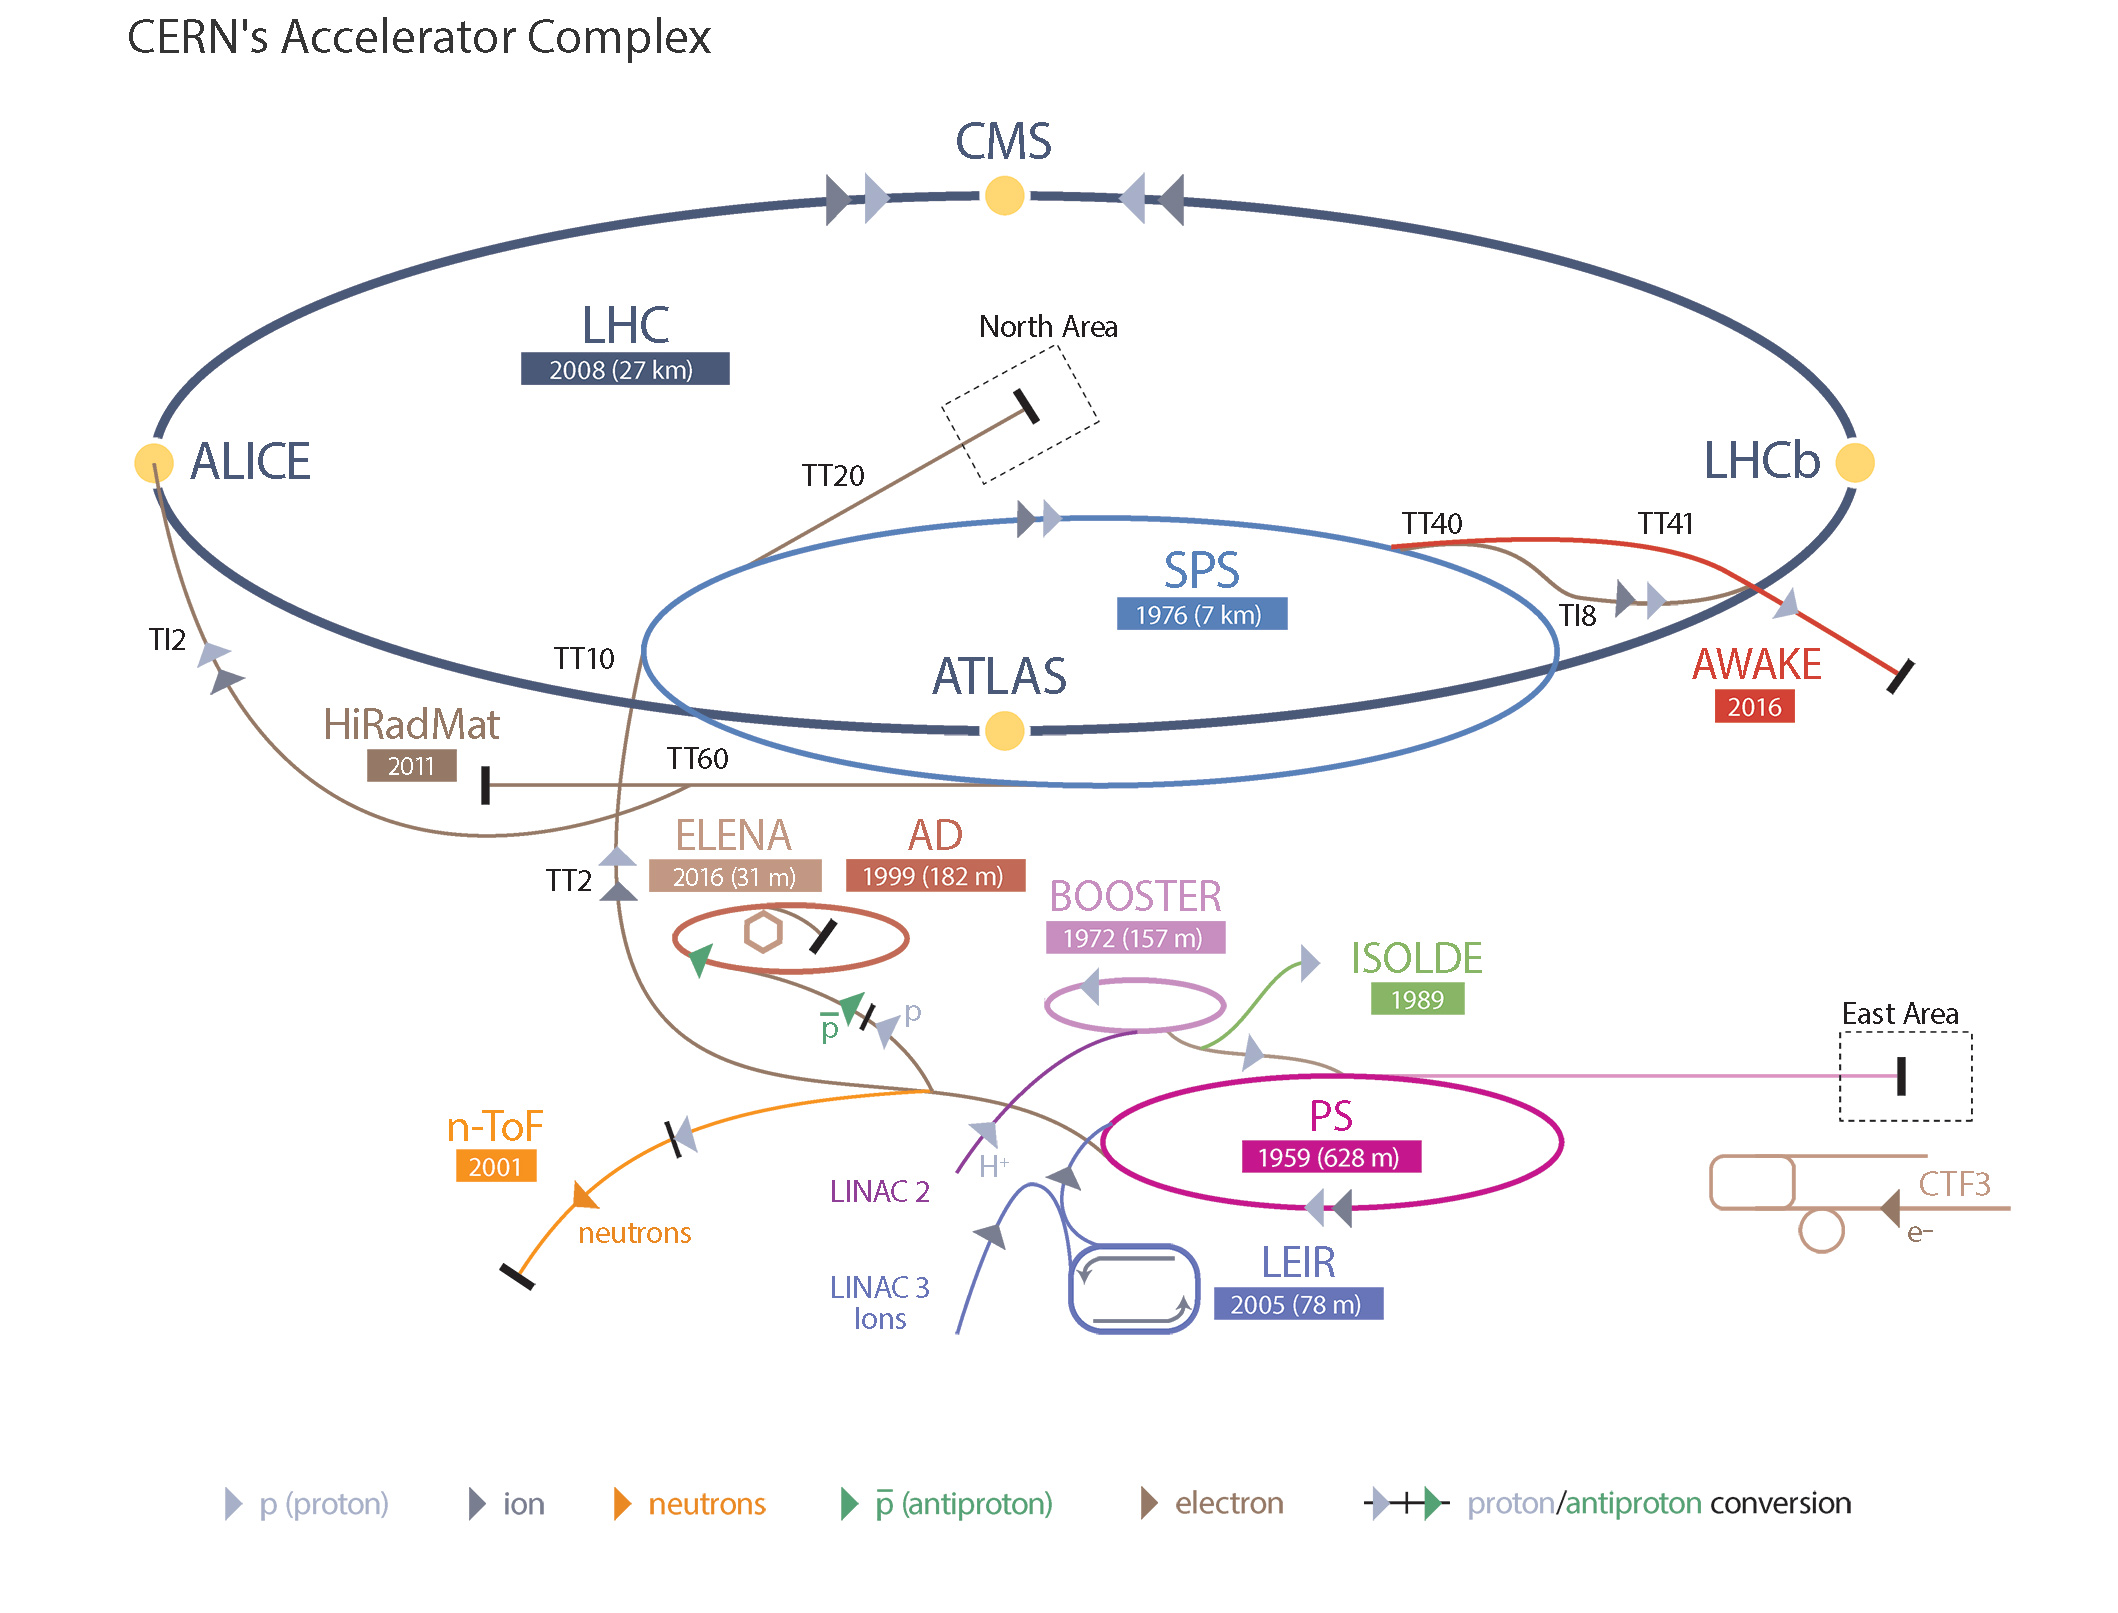
\includegraphics[width=0.8\textwidth]{figures/chapter2/cern_accelerator_complex2}
        \caption{
            Illustration of the various beamlines, accelerator and storage rings, and experimental
            points that the CERN accelerator complex is home to.
            The protons that circulate through the LHC, and that are eventually made to collide inside
            the ATLAS detector, follow the path: Linac 2 $\rightarrow$ Booster $\rightarrow$ Proton Synchotron (PS)
            $\rightarrow$ Super Proton Synchotron (SPS) $\rightarrow$ LHC.
        }
        \label{fig:cern_complex}
    \end{center}
\end{figure}


%%%%%%%%%%%%%%%%%%%%%%%%%%%%%%%%%%%%%%%%%%%%%%%%%%%%%%%%%%%%%%%%%%%
%%%%%%%%%%%%%%%%%%%%%%%%%%%%%%%%%%%%%%%%%%%%%%%%%%%%%%%%%%%%%%%%%%%
% sub-section describing the LHC
%%%%%%%%%%%%%%%%%%%%%%%%%%%%%%%%%%%%%%%%%%%%%%%%%%%%%%%%%%%%%%%%%%%
%%%%%%%%%%%%%%%%%%%%%%%%%%%%%%%%%%%%%%%%%%%%%%%%%%%%%%%%%%%%%%%%%%%
\section{The Large Hadron Collider}
\label{sec:lhc}

The LHC~\cite{LHCMachine} is a circular particle accelerator, with a 27~kilometer circumference,
located at an average distance of 100 meters beneath the surface of the Earth.
It is nominally used for proton-proton ($pp$) collisions, wherein two counter-rotating
beams of protons are made to collide head-on at specific interaction points (IP) along the 27~kilometer
ring, but can also be run in heavy-ion configurations wherein proton-lead ($p$-Pb) or lead-lead (Pb-Pb)
collisions take place.\footnote{The specific lead (Pb) species used in collisions is $^{208}_{82}$Pb.}\footnote{More rarely, the LHC can also be used to circulate gold (Au) ions.
There are even plans to have proton-oxygen ($p$-O) runs in the future, which will allow
for the LHC experiments to provide research that potentially complements dark matter research
based on cosmic-ray air showers.}
The $pp$ collisions take priority over those of the heavy-ions, with the collisions each year
consisting of only a few weeks in the winter for the heavy-ion configurations and typically
six to seven months for the $pp$ configuration. The LHC is designed to accelerate protons to a
center-of-mass energy of $\sqrt{s} = 14\,\TeV$.

\subsection{Machine Design and Layout}
\label{sec:lhc_layout}

\paragraph{Machine Composition} \mbox{} \\
\label{sec:dipole}
The LHC was planned as the successor to the Large Electron Positron (LEP) collider~\cite{LEPI,LEPII}, which was in operation
between the years of 1989 to 2000. LEP is still the most powerful lepton collider to date, having maximal electron-positron
center-of-mass collision energies of 209\,\GeV.
After LEP, the particle physics community knew that the next collider at CERN needed to have $\mathcal{O}(10)$\,\TeV~collision
energies; either to be able to probe from all angles any new physics discovered at LEP and/or the Tevatron~\cite{TevatronDesignI}, or
to provide the necessary power to search for still-elusive hints of BSM physics. At the very least,
given a non-discovery of the Higgs boson at LEP and the Tevatron, the community would need a discovery machine powerful enough
to produce electroweak-scale Higgs bosons and an $\mathcal{O}(10)$ \TeV~hadron collider --- as we now know --- is sufficient for this job.


In order to increase center-of-mass collisions energies, collider designs can take two routes: they can
either increase in size, that is, have larger circumferences (radii), or they can increase the strength of the magnetic
fields used to keep the circulating charged particles in orbit. This can be seen by first considering the expression
for the relativistic cyclotron frequency, $\omega$, of a particle moving in a circular orbit,
\begin{align}
    \omega = \frac{qB}{\gamma m},
    \label{eq:rel_cyclotron}
\end{align}
where $m$ is the particle's rest mass, $B$ is the magnitude of the magnetic field experienced by the
particle, $q$ is the particle's electric charge, and $\gamma$ is the relativistic Lorentz factor, $\gamma = \sqrt{1 - \beta^2} = \sqrt{1 - (v/c)^2}$,
with $v$ the particle's velocity and $c$ the speed of light.
Using Eqn.~\ref{eq:rel_cyclotron}, it can be seen that a particle of higher energy confined to a fixed
circular orbit necessarily has a higher angular velocity by relating the particle's angular
velocity to its kinetic energy:
%A particle of higher energy confined
%to a fixed circular orbit necessarily has a higher
%angular velocity, which can be seen by the expression relating the above angular velocity of the particle to its kinetic energy:
\begin{align}
    E_{\text{kin}} \propto m v^2 = m(\omega R)^2 = \frac{q^2 B^2 R^2}{m \gamma^2}.
    \label{eq:kinetic_energy_gen}
\end{align}
In planning the construction of the LHC, the costs in civil engineering and real-estate works that would
be required to construct a larger tunnel in which to house the LHC ring (increasing $R$) far outweighed
the costs of research into and development of magnet systems strong enough to bend the
multi-\TeV~particles along the beam orbit prescribed by the already-existing LEP tunnel (increasing $B$).
The desired center-of-mass collision energy of $\mathcal{O}(10)$\,\TeV, the fact that the LHC would be a hadron (proton)
collider, and the fact that the LHC would be using the existing LEP tunnel dictate the required magnetic
field strength needed to keep the protons in stable orbits at the LHC. This
is seen by using Eqn.~\ref{eq:kinetic_energy_gen}, solving for $B$, and comparing the LHC and LEP
design parameters,
\begin{align}
    \hspace{-0.4cm}
    \frac{B^2_{\text{LHC}}}{B^2_\text{LEP}} &= \frac{ (E_{\text{LHC}} m_{\text{LHC}} \gamma_{\text{LHC}}^2) / (q_{\text{LHC}}^2 R_{\text{LHC}}^2)  } { (E_{\text{LEP}} m_{\text{LEP}} \gamma_{\text{LEP}}^2) / (q_{\text{LEP}}^2 R_{\text{LEP}}^2) } \label{eq:lhc_mag_field} \\
        &= (E_{\text{LHC}} / E_{\text{LEP}}) \times (m_{\text{LHC}} / m_{\text{LEP}}) \times (\gamma_{\text{LHC}}^2 / \gamma_{\text{LEP}}^2) \times (q_{\text{LEP}}^2 / q_{\text{LHC}}^2) \times (R_{\text{LEP}}^2 / R_{\text{LHC}}^2) \notag \\
        &\approx ( 1\,\TeV~/0.2\,\TeV) \times (m_p/ m_e) \times (1) \times (1) \times (1) \notag \\
        &\approx 10^4 \notag,
\end{align}
which shows that the strength of the LHC bending magnets must be on the order of $100\times$
the strength of those used at LEP. The magnetic fields experienced by the electron and positron beams
at LEP were 0.22 Tesla. By Eqn.~\ref{eq:lhc_mag_field}, the LHC bending magnets should achieve magnetic field
strengths on the order of 10 Tesla in order to achieve the desired collision energies.
The maximum achievable magnetic field of conventional ferrormagnets is about 2 Tesla.
To meet the $\sqrt{s}\approx$10\,\TeV~design goal, the magnet system used by the LHC to confine the protons to their circular orbits
must then be composed of \textit{superconducting} electromagnets. %\footnote{Note that even though
%the main dipole bending magnets at LEP were not superconducting, its focusing quadrupole magnets
%\textit{were} superconducting. There are simply fewer quadrupole magnets, as compared to the number of
%dipole magnets, required for a particle collider.}
The entire magnet system of LEP was therefore removed and replaced with superconducting
niobium-titanium (Nb-Ti) alloy based electromagnets which are superconducting
at temperatures below $10$\,K.
%All of the magnets at the LHC are constructed with
%current carrying elements composed of a niobium-titanium (Nb-Ti) alloy that becomes superconducting
%for temperatures below $10$\,K.
To reach temperatures below this $10$\,K threshold, the LHC magnets
are housed in cryostats that allow for the Nb-Ti elements to be fully submerged in a bath
of superfluid Helium at a temperature of $1.9$\,K~\cite{Casas:1992nf}.
In total, the LHC contains more than 120 tonnes of superfluid Helium.
It goes without saying that there is a significant amount of resources and person power at CERN devoted to the refrigeration and cryogenics
systems that are required for the LHC to run.

Additionally, the fact that LEP was a \textit{particle-antiparticle} collider meant that the counter-rotating
beams could be made to occupy a single ring: the same magnetic field could produce counter-rotating beams of
electrons and positrons within the same beam pipe.\footnote{The electrons and positrons at LEP were vertically separated
within the beam pipe by electrostatic separators placed throughout the LEP ring. Turning off these separators
is, to first approximation, how the LEP operators would get the electrically-attracting electrons and positrons to collide.}
As a result, the LEP beam tunnel was constructed with only a single ring in mind and is relatively narrow: the LEP tunnel,
and therefore LHC tunnel, is only $\approx$3.7\,m wide on average.
As the LHC is a \textit{particle-particle} collider, it necessarily requires \textit{two} magnetic fields
of opposing polarity to circulate one of its beams in the clockwise direction and the other in the
counter-clockwise direction.
Given the limited space in the tunnel, however, it is not possible to house two separate rings
of superconducting bending magnets with all of the services that they require \textit{in addition} to the requisite
minimal space needed for personnel and maintenence access.
This forced the need of the so-called `2-in-1' design of the main bending magnets of the LHC, wherein the two
beam pipes are housed in the same cryostat in which the counter-rotating beams are held in their
respective orbits by coupled magnetic fields.
An illustration of this now-iconic design of the LHC bending (dipole) magnets and surrounding cryostat and containment structure is illustrated in Figure~\ref{fig:lhc_dipole_xsec}.
Each of the 15\,meter long superconducting dipole electromagnets of the LHC responsible for constraining the protons to their circular
orbits has currents of $11850$\,Amperes flowing through it and achieves magnetic field strengths of $8.33$\,Tesla.

\begin{figure}[!htb]
    \begin{center}
        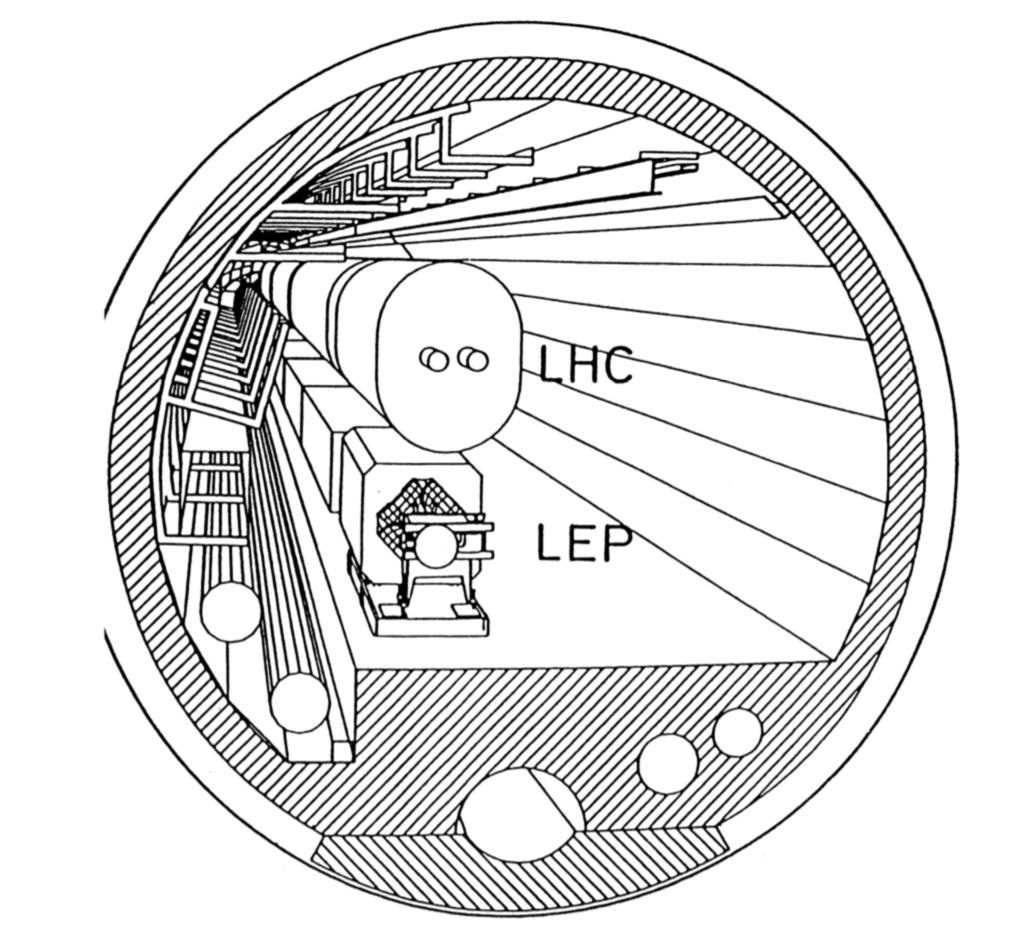
\includegraphics[width=0.43\textwidth]{figures/chapter2/lhc_lep_dipole_comp}
        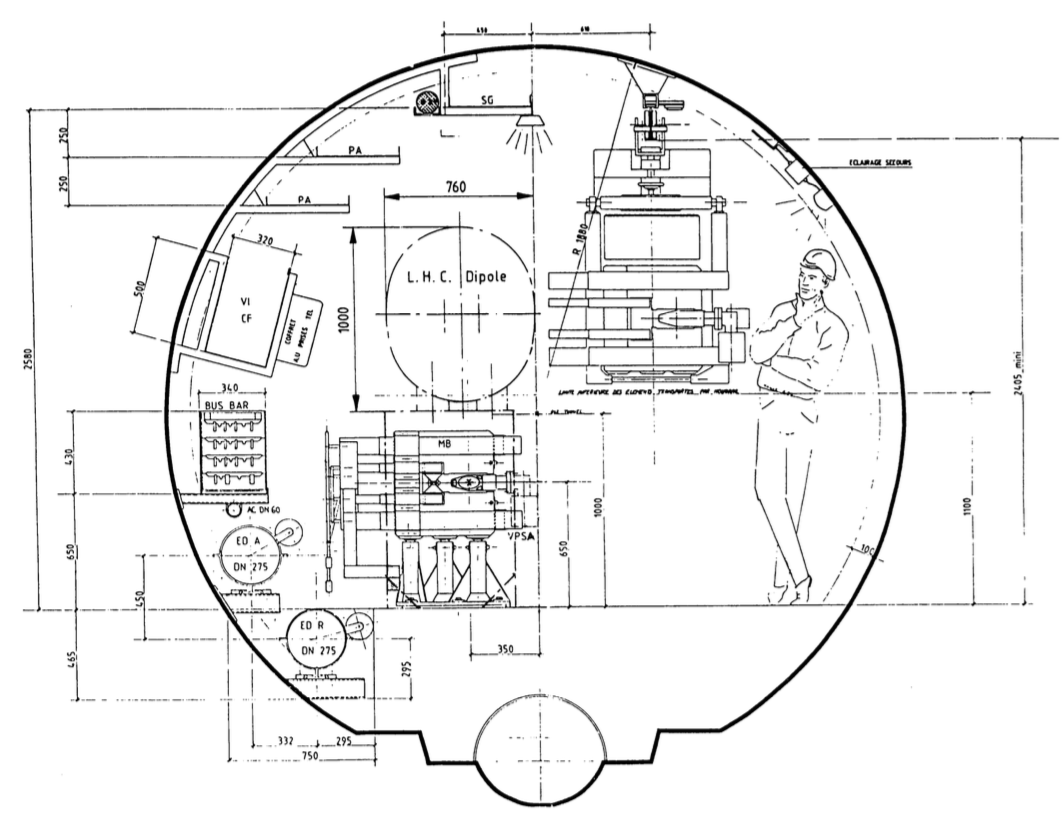
\includegraphics[width=0.50\textwidth]{figures/chapter2/lhc_lep_dipole_comp_person}
        \caption{
            \textit{Left}: Illustration comparing the size of a `2-in-1' LHC dipole configuration to the
                LEP dipole and how they fit inside of the LEP/LHC tunnel. Note that prior to LHC operation,
                the LEP magnets will have been removed: the two are shown side-by-side for comparison purposes only.
            \textit{Right}: Cross-sectional view of the LEP/LHC tunnel with a comparison of the LHC `2-in-1' dipole
                on top of the LEP dipole. An illustration of an average size person is shown
                for scale. Also shown is the service crane in use, to give an idea of the size required
                for potential maintenance access. Clearly, two single-bore, superconducting rings each similar in size
                to the LEP dipole would not fit comfortably in the tunnel. The LHC `2-in-1' design fits
                in nearly the same area as the LEP dipoles while additionally being able to contain both
                particle beams.
                Figures are taken from Ref.~\cite{ECFALHCinLEP}.
        }
        \label{fig:lhc_lep_dipole_comp}
    \end{center}
\end{figure}

\begin{figure}[!htb]
    \begin{center}
        \begin{minipage}{\textwidth}
        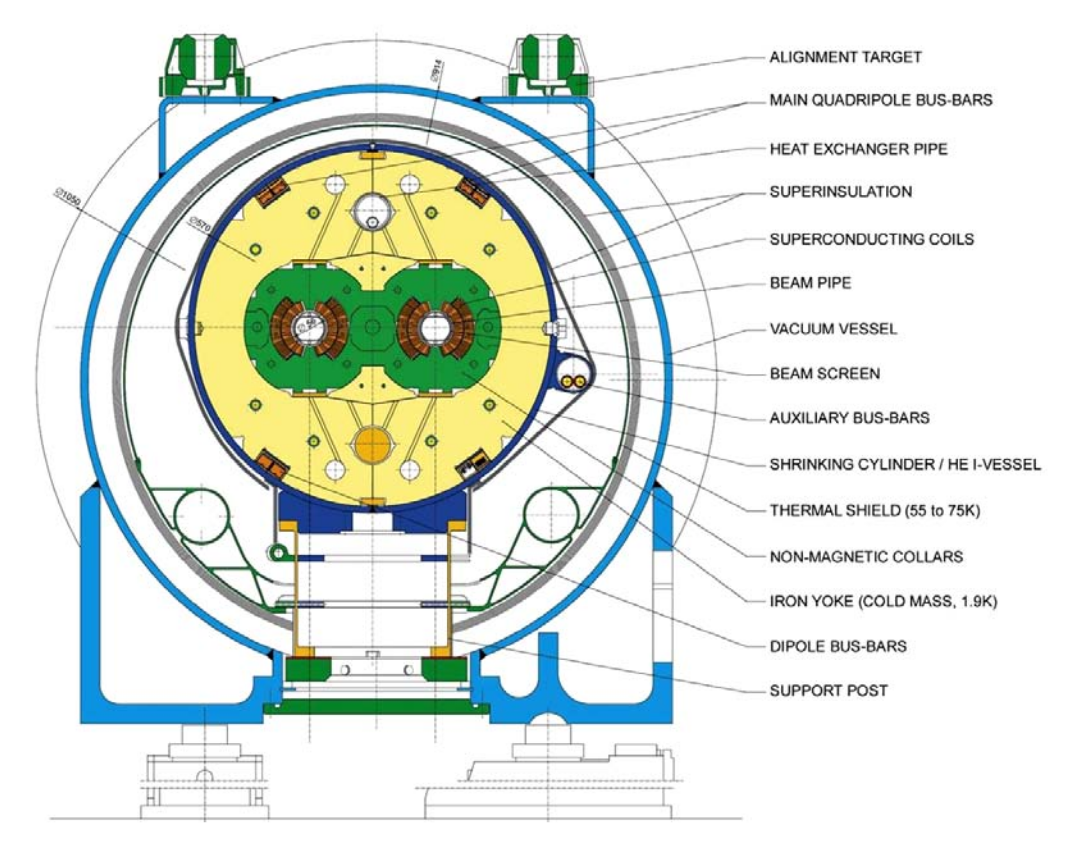
\includegraphics[width=0.59\textwidth]{figures/chapter2/lhc_dipole_fig3p3}
        \raisebox{0.5cm}{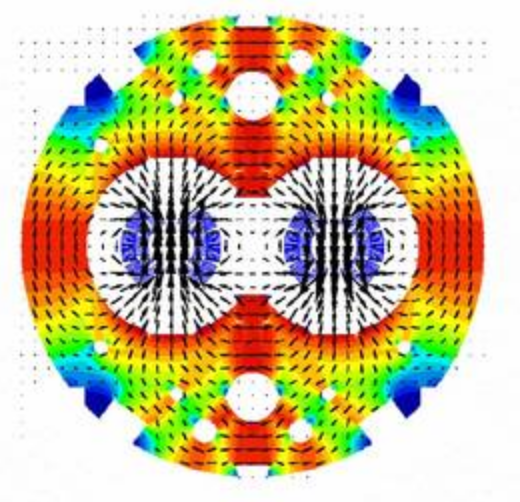
\includegraphics[width=0.4\textwidth]{figures/chapter2/dipole_magnetic_field_lines}}
        \end{minipage}
        \caption{
            \textit{Left}: Cross-sectional view of an LHC dipole bending magnet, with relevant parts indicated.
            The protons orbit inside of the beam pipes, each of which has a diameter of roughly $3$\,cm.
            It is interesting to note that the non-magnetic steel collars (in green) are of critical import
            to the success of the magnet systems. They are required
            to prevent the dipole structure from being deformed or torn apart due to the intense magnetic forces
            tending to push the two beam-pipes apart as a result of their counter-rotating electromagnetic currents.
            These forces amount to about 400 tonnes per meter of dipole when in full operation --- almost equivalent in magnitude
            to the weight of a Boeing 747.
            \textit{Right}: Magnetic field lines of the coupled dipole fields that bend the counter-rotating proton beams
            and keep them in their circular orbits around the LHC ring.
        }
        \label{fig:lhc_dipole_xsec}
    \end{center}
\end{figure}


%\FloatBarrier
\paragraph{Connecting the Dots} \mbox{} \\
The LHC is essentially a chain of superconducting magnets of the type described in the previous paragraphs, where
the the bending (dipole) magnets critical to the LHC design were introduced.
%There are additional
%types of magnets that produce fields of higher multipole moments which, in the case of the quadrupole magnets, are
%necessary for beam \textit{beam focusing}. Conceptually they are very similar to the dipoles and are 
The chain is laid in a double-octagonal structure, illustrated in Figure~\ref{fig:lhc_layout}. There are eight
octants, at the center of which the LHC ring is straight and does not curve.
The LHC curvature occurs at the
boundaries of each of the octants and is primarily made up of bending (dipole) magnets.
The straight sections are where the interaction regions are located and are referred
to as `Points', numbered 1 to 8.
Points 1, 2, 5, and 8 are where the four large LHC experiments are located.
Points 1 and 5 are home to the services and underground areas
of the general purpose experiments, ATLAS and CMS, respectively.
The underground experimental caverns associated with Point 1 and 5 were not present for LEP and
had to be constructed after LEP was retired in 2000.
Figure~\ref{fig:p1} provides an illustration of how the surface and underground
areas are situated at Point 1.
Points 2 and 8 host the services and underground areas of the ALICE and LHCb experiments, respectively.
At these Points, Points 1, 2, 5, and 8, the counter-rotating beams are
made to collide. The remaining Points, Points 3, 4, 6, and 7, are host to various beam `services'
necessary for the operation of the LHC.
Point 3 and 7 host the beam betatron and momentum cleaning (`beam collimation') systems, respectively.
Point 4 hosts the superconducting radio-frequency (RF) systems which accelerate the beams to
their nominal collision energies.
Point 6 is the location of the beam-abort system --- the so-called `beam dump' --- where
the LHC beams may be removed very quickly from the LHC ring by using \textit{kicker} magnets~\cite{LHCDesignI}
that divert the beams out of the LHC ring in a safe manner. The beams may be dumped
if the LHC wishes to refill with protons (or heavy-ions) and needs to remove any
remnants of the previous fill, in case of beam instabilities observed in the LHC ring,
or if one of the experiments signals the need for a beam dump (in case of
beam stability or detector issues observed at the associated IP).

\begin{figure}[!htb]
    \begin{center}
        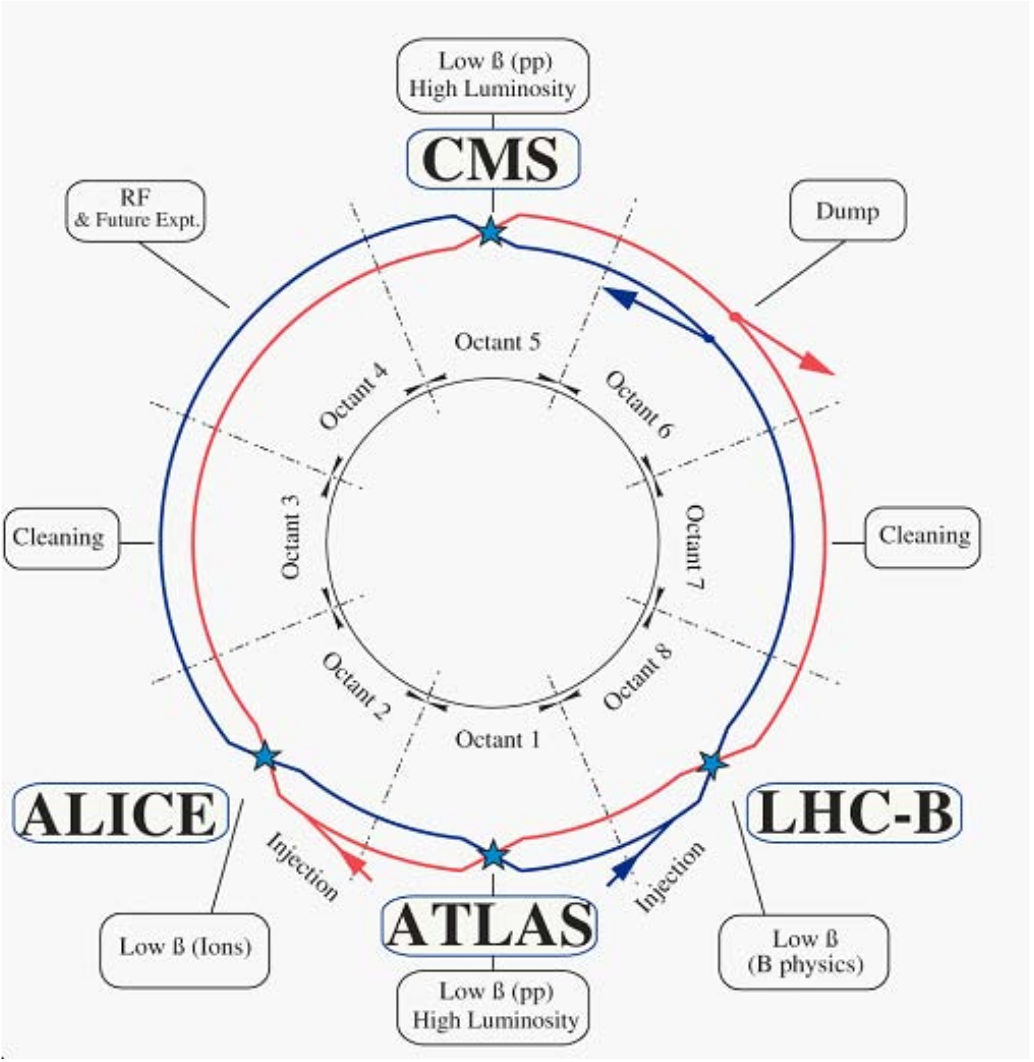
\includegraphics[width=0.8\textwidth]{figures/chapter2/lhc_layout}
        \caption{
            Layout of the LHC and its two counter-rotating beams. Beam 1 is in blue and rotates
            counter-clockwise. Beam 2 is in red and rotates clock-wise.
            At the center of each octant is a straight section which houses
            the experimental caverns or LHC beam facilities.
            At the boundaries of each octant are located the curved sections.
            Figure taken from Figure 2.1 of Ref.~\cite{LHCMachine}.
            {\color{red}{Somewhere $\beta$ should be described -- betatron function}}
        }
        \label{fig:lhc_layout}
    \end{center}
\end{figure}

\begin{figure}[!htb]
    \begin{center}
        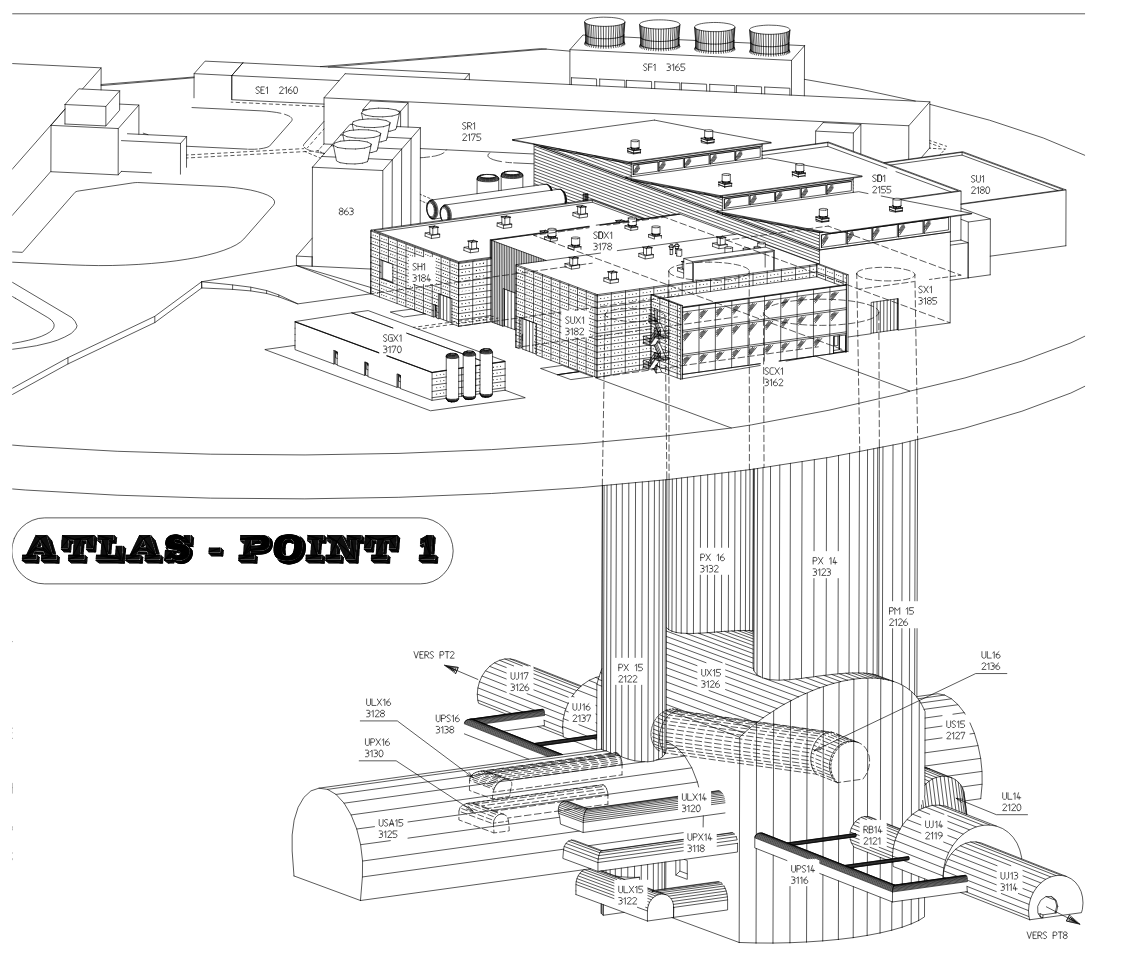
\includegraphics[width=0.75\textwidth]{figures/chapter2/point1_illustration}
        \caption{
            Diagram showing the surface buildings and services and underground areas of Point 1, where
            the ATLAS experiment is located. The LHC ring can be seen at the bottom,
            with its directions indicated by the `VERS PT8 (2)' arrows pointing
            towards Point 8 (2).
            The experimental cavern in which the ATLAS detector sits is UX15.
            The control room for the ATLAS experiment, whereat operators can monitor and
            control the state of the ATLAS detector, is located 100\,m above
            UX15 in the building SCX1.
            Figure taken from Figure 10.1 of Ref.~\cite{LHCDesignII}.
        }
        \label{fig:p1}
    \end{center}
\end{figure}

%\FloatBarrier
\subsection{Injection Chain and Bunch Structure}
\label{sec:lhc_injection}

We now have an idea of how the proton beams relevant to the work
in this thesis are made to circulate in the LHC ring.
In this section we will briefly describe the initial source of the protons and how
they are introduced into the LHC ring.
The LHC relies on a series of pre-acceleration steps that bring the initial
low-energy protons to energies sufficient enough to begin their journey through the LHC.
The sum-total of these steps is referred to as the LHC \textit{injection chain}~\cite{LHCDesignIII}.
The components of the LHC injection chain form the heart of the CERN accelerator
complex illustrated in Figure~\ref{fig:cern_complex}.
For $pp$ collisions in the LHC, the protons are initially sourced from Hydrogen atoms that are released
at the start of Linac 2.
The Hydrogen atoms are immediately stripped of their electrons after passing through
the \textit{duoplasmatron} ion source~\cite{Duoplasma}.
The protons are then passed through Linac 2, a linear accelerator, which accelerates
the protons to $50$\,\MeV.
They then enter the Proton Synchotron Booster (PSB), a circular storage ring
composed of four stacked rings, which accelerates the protons to $1.4\,\GeV$.
The PSB injects the protons into the Proton Synchotron (PS) which accelerates
them to $25$\,\GeV.
The Super Proton Synchotron (SPS) receives the protons from the PS and
accelerates them to $450$\,\GeV.
At this point the protons have sufficient energy to be injected into the LHC.
There are two injection points into the LHC since, up until this stage,
the protons are circulating in the same direction: one injection point sends
protons into the counter-clockwise beamline of the LHC, and the other
into the clockwise beamline.
Until all of the protons from a single \textit{fill} make their way into
the LHC, they will circulate at the injection energy of $450$\,\GeV.
After the filling completes\footnote{A standard LHC fill takes on the order of 4 minutes per
ring.}, the superconducting RF cavities located at Point 4 will begin to accelerate the protons
to their final collision energies.\footnote{If all goes smoothly, this acceleration stage takes roughly 20 minutes.}
The acceleration is achieved by increasing the frequency of the RF oscillations; however,
given that a $450$\,\GeV~proton is already ultra-relativistic, the adjustment of the frequency
needed to get to the collision energies is not large.

The proton beams circulating the LHC are not a continuous stream of protons; rather,
they are grouped into what are referred to as \textit{bunches}.
The protons arrive at the LHC in these bunches which are initially prepared
in the smaller machines that make up the LHC injection chain and then are
kept in their final \textit{bunch structure} by the RF cavities.
The accelerating RF cavities provide an accelerating electromagnetic field
that oscillates longitudinally. The bunches, each composed of roughly $10^{11}$ protons,
are then made to oscillate longitudinally in so-called \textit{synchotron oscillations}
around the central node of the RF oscillation as they circulate through the LHC ring.
The proton bunches are then effectively `shaped' by the oscillating RF field: protons in a bunch
lagging behind or that are ahead of those particles at the center of the bunches
will be accelerated or decelerated accordingly so as to be pushed back into the center of the bunch.
The LHC RF cavities have an oscillation frequency of $400$\,MHz which
defines the boundaries in which proton bunches can lie. These boundaries are
called \textit{RF buckets} and, along with
the circumference of the LHC, dictate the number of proton bunches that
can potentially fit in the LHC.
The relationship between the RF oscillations and the RF bucket and bunch structure
is illustrated in Figure~\ref{fig:lhc_bunch}.
In total, approximately 35640 RF buckets exist when the LHC is in operation.
Not all buckets contain proton bunches, however.
In fact, at the time of the writing of the present thesis,
RF buckets filled with proton bunches have a minimal separation of 10 RF buckets, meaning
that following an RF bucket containing a proton bunch there is at least 9 unfilled RF buckets.
This corresponds to a minimal
time between proton bunches --- the \textit{bunch spacing} --- of $25$\,nanoseconds.
At the time of the present thesis, the operating conditions of the LHC maximally
allow for 2808 $25$\,ns-spaced bunches.\footnote{
The number of allowed bunches is significantly lower than the 35640 RF buckets with $25$\,ns
bunch-spacing potentially allow for. This is due, in part, to the non-trivial bunch-structure
typically employed but also in large part to the fact that there is a rather long \textit{abort gap}
in the LHC ring where no filled RF buckets exist.
The abort gap is a number of continuous unfilled RF buckets that allows the ramp up of the kicker
magnets used for the beam dump to occur in the absence of filled buckets.
In this way, the kicker magnet ramp up does not disturb the structure of the circulating proton beams.
Only after this ramp up is finished should the kicker magnets disturb the beams.
}
The bunch-spacing and overall bunch structure of an LHC fill is not only decided
by the operators of the LHC but also by what the detectors at Points 1,2,5, and 8
can tolerate. This is because shorter bunch spacing means higher intensity and multiplicity
of collisions occuring at each of these IP. A $25$\,nanosecond bunch spacing
corresponds to a maximal $pp$ collision rate of $40$\,MHz. The detectors at each
of the IP have been designed with this collision rate in mind and anything
higher may push them beyond their design limits.

\begin{figure}[!htb]
    \begin{center}
        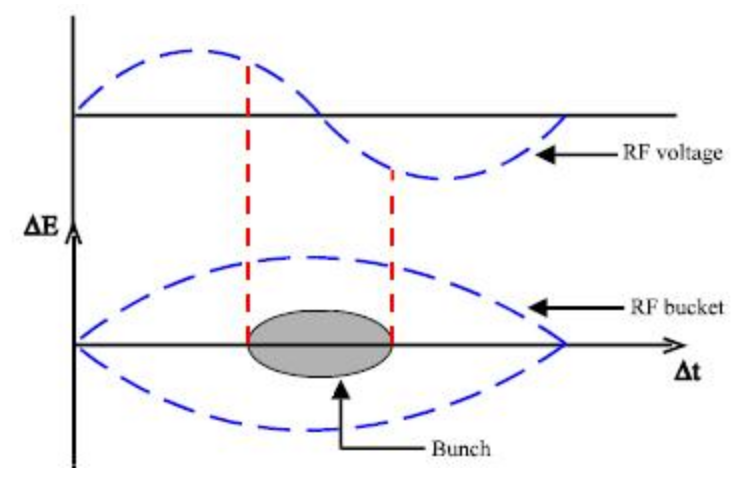
\includegraphics[width=0.5\textwidth]{figures/chapter2/lhc_bunch}
        \caption{
            Illustration of the particle bunch structure in a particle collider such as the LHC.
            The particles are accelerated by radio-frequency (RF) oscillations whose
            amplitude is illustrated in the upper plot.
            The RF bucket's boundary, illustrated in the lower plot, is defined by a full period of the RF oscillation
            and the particle bunch formation, depicted in grey, occurs at the central node of the oscillation.
            The area occupied by the particle bunch is related to the beam's longitudinal
            \textit{emittance}.
        }
        \label{fig:lhc_bunch}
    \end{center}
\end{figure}

\subsection{The Concept of Luminosity}
\label{sec:lhc_luminosity}

In designing a particle collider, the collision energy is not the only important parameter.
Equally important is the value of the instantaneous \textit{luminosity}
that can be achieved by the collider.
An expression for the instantaneous luminosity, $\mathcal{L}$, is given by,
\begin{align}
    \mathcal{L} = \frac{N^2 n_b f}{4 \pi \sigma_x \sigma_y} \cdot S,
    \label{eq:luminosity}
\end{align}
where $N$ is the number of particles per bunch, $n_b$ is the number of colliding bunches,
$f$ is the bunch revolution frequency, $\sigma_{x,y}$ are the transverse beam widths in the
Gaussian approximation, and $S$ is a reduction factor that accounts for geometric factors
such as the non-zero crossing-angle of the colliding beams~\cite{LHCDesignIII,LumiConcept}.
The instantaneous luminosity, $\mathcal{L}$, can be seen by Eqn.~\ref{eq:luminosity}
to have units of cm$^{-2}$s$^{-1}$ and can be conceptually thought of as the
outgoing flux of particles per unit area and time after a bunch crossing in which successful $pp$
collisions occur.
The LHC is designed to deliver collisions to the high luminosity IP (Fig.~\ref{fig:lhc_layout})
at $\mathcal{L} = 10^{34}$\,cm$^{-2}$s$^{-1}$.
Accurate knowledge of $\mathcal{L}$ is of the utmost importance for collider design and operation.
Not only does it parametrise the potential collision rate once the collider beam and bunch
structure are decided, but it allows for the accurate prediction of the number
of collision events, $N_{\text{proc}}$, associated with a particular physics process
with cross-section $\sigma_{\text{proc}}$,
\begin{align}
    N_{\text{proc}} = \sigma_{\text{proc}} \int \mathcal{L}\, \mathrm{d}t \equiv \sigma_{\text{proc}} \cdot L,
    \label{eq:n_exp_lumi}
\end{align}
where $L$ is referred to as the \textit{integrated luminosity} and has units of cm$^{-2}$.
A common unit for integrated luminosity is the \textit{barn}, with symbol `b': one barn is defined as $10^{-24}$\,cm$^{-2}$.
The datasets collected by the LHC experiments are such that the \textit{femtobarn} (fb), $10^{-39}$\,cm$^{-2}$, is relevant.

\subsection{Operation of the Large Hadron Collider}
\label{sec:lhc_operation}

The LHC has been in stable operation since 2009.
It operates in so-called \textit{runs}: multi-year periods of roughly continuous
data-taking.
As CERN shuts down during the winter months, each run is segmented each year
with a several month long shutdown in the winter with a ramp-up period in the spring.
During these shorter shutdowns, maintenance and upgrades may also take place.
In between a given run there is a multi-year break, a \textit{long shutdown},
in which large(er)-scale maintenance and upgrades of both the LHC and the experiments can take place.
At the time of writing, there has so far been two runs of the LHC, Run-I and Run-II.
Run-I took place during the years 2009--2012 and Run-II during 2015--2018.
The integrated luminosities for each of the data taking years between Run-I and Run-II
is shown in Fig.~\ref{fig:int_lumi_multiyear}.
The data relevant to the work presented in this thesis were collected in both
Run-I and Run-II of the LHC, specifically that data collected in the years 2012--2018.
The luminosities, instantaneous and integrated, as well as the center-of-mass collision energies, $\sqrt{s}$, for these data-taking periods are
shown in Table~\ref{tab:lumi_tab}.
Also shown in Table~\ref{tab:lumi_tab} are the average values of the mean number of interactions per bunch
crossing, $\langle \mu \rangle$, observed during each data-taking year. The quantity $\langle \mu \rangle$
is related to the amount of \textit{pileup} observed during data-taking. Pileup is caused
by overlapping $pp$ interactions within the same (\textit{in-time} pileup) or neighboring (\textit{out-of-time} pileup)
bunch-crossing(s) at the interaction point. The pileup scales with the instantaneous luminosity.
Distributions of $\langle \mu \rangle$ are shown in Fig.~\ref{fig:int_lumi_multiyear} for
the Run-II data-taking period.


\begin{table}[!htb]
    \begin{center}
        \begin{tabular}{l | c | c c c c }
        \hline
        \hline
        & \textbf{Run-I} & \multicolumn{4}{c}{\textbf{Run-II}} \\
        \hline
        Year & 2012 & 2015 & 2016 & 2017 & 2018 \\
        \hline
        Collision energy, $\sqrt{s}$ [TeV] & 8 & \multicolumn{4}{c}{13} \\
        Peak Luminosity, $\mathcal{L}$ [cm$^{-2}$s$^{-1}$] ($\times10^{34}$) & $0.77$ & $0.5$ & $1.4$ & $2.1$ & $2.1$ \\ 
        Integrated Luminosity, $L$ [fb$^{-1}$] & 20.2 & 3.2 & 33.0 & 44.3 & 59.9 \\
        Mean number of of interactions & & & & & \\
        \hspace{1.7cm} per bunch crossing, $\langle \mu \rangle$ & 20.7 & 13.4 & 25.1 & 37.8 & 36.1 \\
        \hline
        \hline
        \end{tabular}
        \caption{
            Summary parameters for the data-taking periods relevant to the work
            presented in this thesis. The integrated luminosity is that relevant
            to performing physics analysis and potentially differs with respect to
            the total integrated luminosity delivered to ATLAS by the LHC (Fig.~\ref{fig:int_lumi_multiyear}) due to
            the application of strict quality criteria on the data prior to its use
            in physics analyses.
        }
        \label{tab:lumi_tab}
    \end{center}
\end{table}

\begin{figure}[!htb]
    \begin{center}
        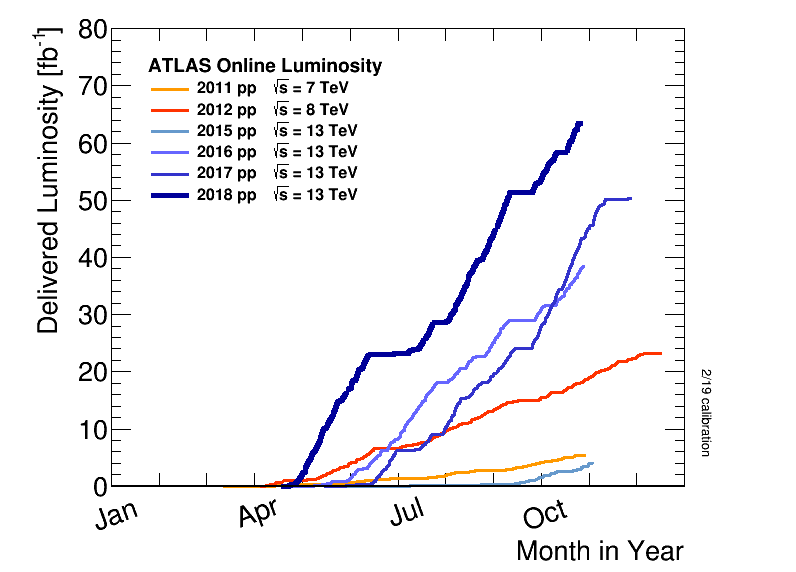
\includegraphics[width=0.49\textwidth]{figures/chapter2/int_lumi_multiyear}
        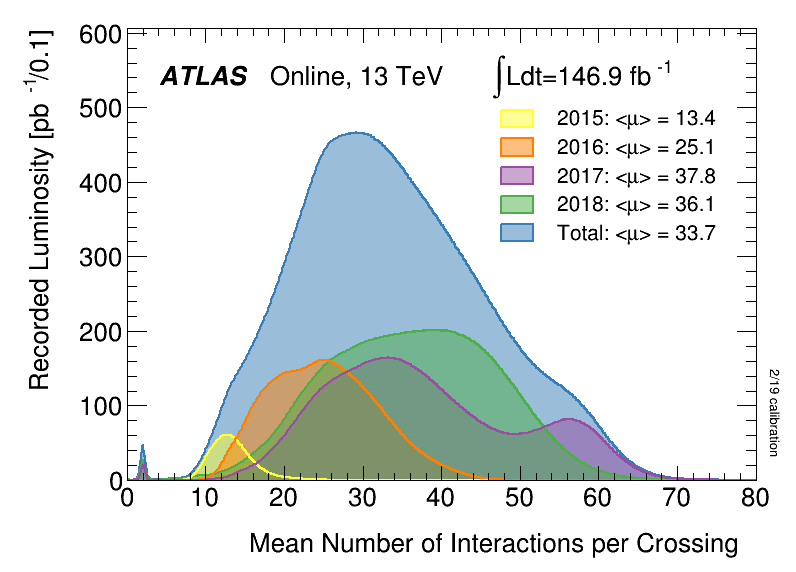
\includegraphics[width=0.49\textwidth]{figures/chapter2/mu_run2}
        \caption{
            \textit{Left}: The ATLAS integrated luminosity during the data-taking years 2011--2018.
            \textit{Right}: The observed average number of $pp$ interactions per bunch-crossing, $\langle \mu \rangle$,
                observed by ATLAS during the Run-II data-taking years, 2015--2018.
        }
        \label{fig:int_lumi_multiyear}
    \end{center}
\end{figure}


%%%%%%%%%%%%%%%%%%%%%%%%%%%%%%%%%%%%%%%%%%%%%%%%%%%%%%%%%%%%%%%%%%%
%%%%%%%%%%%%%%%%%%%%%%%%%%%%%%%%%%%%%%%%%%%%%%%%%%%%%%%%%%%%%%%%%%%
% sub-section describing ATLAS
%%%%%%%%%%%%%%%%%%%%%%%%%%%%%%%%%%%%%%%%%%%%%%%%%%%%%%%%%%%%%%%%%%%
%%%%%%%%%%%%%%%%%%%%%%%%%%%%%%%%%%%%%%%%%%%%%%%%%%%%%%%%%%%%%%%%%%%
\section{The ATLAS Detector}
\label{sec:atlas}

In this section we will extend our focus to the ATLAS detector, the general purpose
particle detector located at Point 1 of the LHC ring (see Figure~\ref{fig:p1}).
Roughly cylindrical in shape, coaxial with the beam-pipe,
the ATLAS detector is 44\,m long and 25\,m tall.
It is by far the largest such detector ever built and,
generally, is the largest and most complex device ever constructed.
Being general purpose in scope, the ATLAS detector is hermetic and has
nearly $4\pi$ radians of solid angle coverage around the $pp$ collision
point. 
Such detectors are commonly designed to have various subsystems --- \textit{subdetectors} ---
which are designed for the identification of specific types of particles
and interactions.
They tend to be layered about the interaction point and cylindrically symmetric
since the $pp$ interactions taking place within the detector have no preferred
direction in the plane transverse to the direction in which the proton beams
are travelling.
A view of the ATLAS detector and its subdectors is provided by Figure~\ref{fig:atlas_cutaway}.
In the following we will briefly describe each subsystem in turn, describing
first the detectors located nearer to the $pp$ collision and proceeding outwards.

\subsection{The ATLAS Coordinate System}
\label{sec:atlas_coordinate_system}

The ATLAS detector uses a right-handed coordinate system with the origin located at
the geometric center of the detector.
The $x$-axis points to the center of the LHC ring, the $y$-axis points upwards
and away from the center of the Earth, and the $z$-axis is along the beam-pipe.
The side associated with positive (negative) $z$
is referred to as the `A' (`C') side of the detector.\footnote{`A' for `airport',
since this is the side pointing towards Geneva International Airport, and
`C' for either `Crozet' or `Charly's', depending on who you ask, since this is the side
pointing towards the town of Crozet and/or Charly's Pub in the town of Saint-Genis-Pouilly.}
Due to its cylindrical symmetry, ATLAS also uses the cylindrical coordinates, $(r,\phi, z)$,
with $\phi$ the azimuthal angle about the $z$-axis and having $\phi = 0$ along the positve $x$-axis.
The spherical polar angle, $\theta$, is defined with respect to the $z$-axis, having
$\theta = 0$ parallel to the beam-pipe and $\theta = \pi/2$ in the $xy$-plane transverse
to the beam-pipe.
The pseudorapidity, $\eta$, is commonly used when describing systems of particles or locations within
the detector and is defined as $\eta = - \ln \left[ \tan \left( \theta / 2 \right) \right ]$.
The relationship between pseudorapidity and polar angle is illustrated in Figure~\ref{fig:eta_desc}.
Large (small) values of $\eta$ correspond to the \textit{forward} (\textit{central}) region of the detector.
The rapidity, $y$, is related to $\eta$ and is defined as $y = \frac{1}{2} \ln \left[ (E+p_z) / (E-p_z) \right]$.
The pseudorapidity of a particle traversing the detector is equal to its rapidity if
the particle is massless or ultra-relativistic; otherwise, they are different.
The comparison between a particle's pseudorapidity and rapidity is illustrated in
Figure~\ref{fig:eta_desc}.
The coordinates used to describe systems of particles are typically described by their
four-momenta: $(p_x, p_y, p_z)$ or, equivalently, $(\pT, \eta, \phi)$.
A distance metric commonly used to describe the distance between two systems of particles
in the detector is $\Delta R = \sqrt{ (\Delta \eta)^2 + (\Delta \phi)^2 }$. The
$\Delta R$ quantity using $y$ instead of $\eta$ is also sometimes used and will be
indicated by $\Delta R_y$.

\begin{figure}[!htb]
    \begin{center}
        \raisebox{1.5cm}{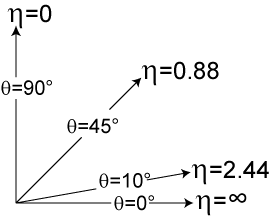
\includegraphics[width=0.35\textwidth]{figures/chapter2/eta_vs_polar}}
        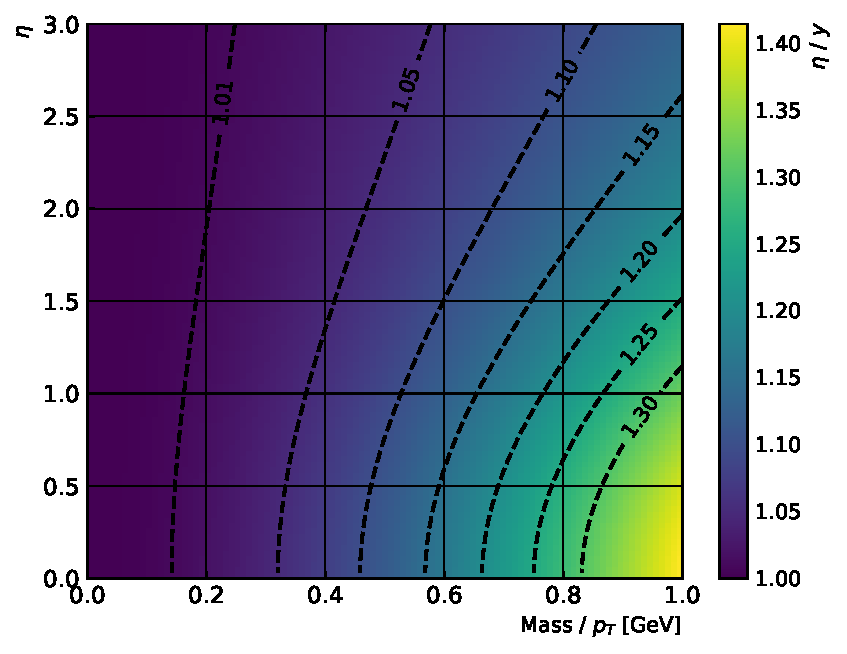
\includegraphics[width=0.55\textwidth]{figures/chapter2/eta_vs_rap}
        \caption{
            \textit{Left}: Illustration of the relationship between the pseudorapidity, $\eta$,
                and polar angle, $\theta$, defined as the angle with respect to the beam-axis ($z$-axis).
            \textit{Right}: Distribution of the ratio of a particle's pseudorapidity to its rapidity, $\eta$/$y$,
                as a function of its pseudorapidity ($y$-axis) and the ratio of its mass to its transverse momentum, \pT~($x$-axis).
        }
        \label{fig:eta_desc}
    \end{center}
\end{figure}


\begin{figure}[!htb]
    \begin{center}
        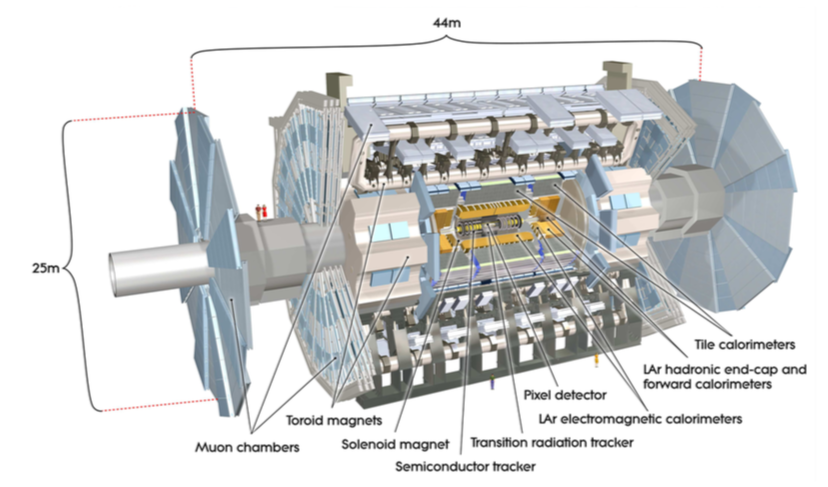
\includegraphics[width=0.95\textwidth]{figures/chapter2/atlas_cutaway}
        \caption{
            Cut-away view of the ATLAS detector with sub-systems indicated.
            Shown for comparison are figures of average-height humans standing
            at the feet of the detector and standing on the forward shielding
            between the big wheels of the forward muon system.
        }
        \label{fig:atlas_cutaway}
    \end{center}
\end{figure}


\begin{figure}[!htb]
    \begin{center}
        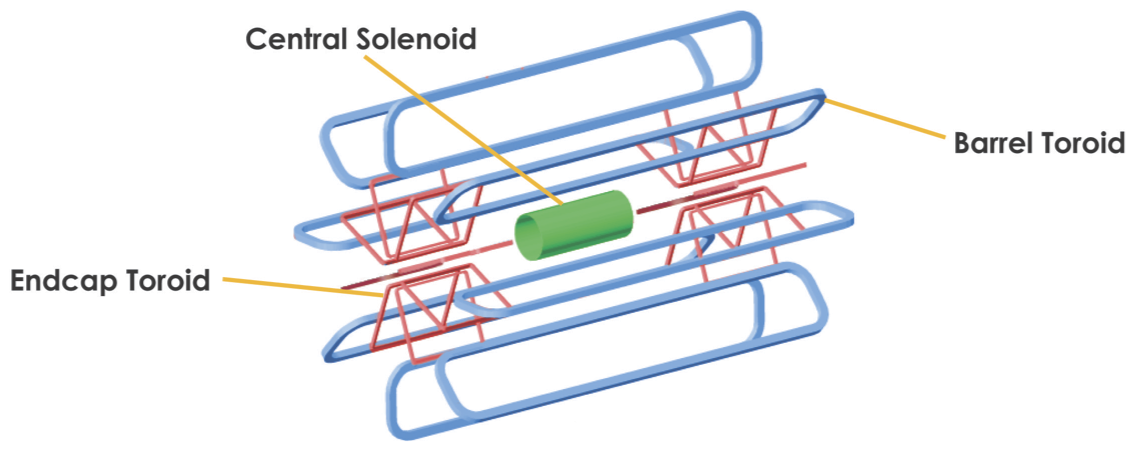
\includegraphics[width=0.95\textwidth]{figures/chapter2/atlas_magnet_system}
        \caption{
            A view of the ATLAS magnet system. Shown are the 2\,T solenoid magnet
            in green, the barrel toroid system in blue, and endcap toroid magnets
            in red.
        }
        \label{fig:atlas_magnet_system}
    \end{center}
\end{figure}

%%%%%%%%%%%%%%%%%%%%%%%%%%%%%%%%%%%%%%%%%%%%%%%%%%%%%%%%%%%%%%%%%%%%%
%%%%%%%%%%%%%%%%%%%%%%%%%%%%%%%%%%%%%%%%%%%%%%%%%%%%%%%%%%%%%%%%%%%%%
%
% INNER DETECTOR
%
%%%%%%%%%%%%%%%%%%%%%%%%%%%%%%%%%%%%%%%%%%%%%%%%%%%%%%%%%%%%%%%%%%%%%
%%%%%%%%%%%%%%%%%%%%%%%%%%%%%%%%%%%%%%%%%%%%%%%%%%%%%%%%%%%%%%%%%%%%%
\subsection{The Inner Detector}
\label{sec:inner_detector}

The innermost subdetector of ATLAS is the Inner Detector (ID)~\cite{Haywood:331064}.
The ID covers the region $\lvert \eta \rvert < 2.5$ and is composed, in order
of increasing radial distance from the beam-pipe, of the pixel detector,
semiconductor tracker (SCT), and the transition radiation tracker (TRT).
These detectors enable the reconstruction of the tracks associated with
the $\mathcal{O}(1000)$ charged particles emerging from each $pp$ bunch collision, occuring
every 25\,ns.
An illustration of the ID and its subdetectors is shown in Figure~\ref{fig:atlas_inner_detector}.
Additional, more detailed views of the barrel and endcap sections of the ID are shown in Figure~\ref{fig:atlas_ID_exploded}.
The ID is situated inside of the central solenoid, indicated in Figure~\ref{fig:atlas_magnet_system},
which provides an axial 2\,T magnetic field and extends over a length of 5.3\,m with a diameter of 2.5\,m.
The bending of charged particles in the $xy$-plane due to the presence of the solenoidal
field allows for their momenta to be measured using the curvature of their reconstructed tracks.

\begin{figure}[!htb]
    \begin{center}
        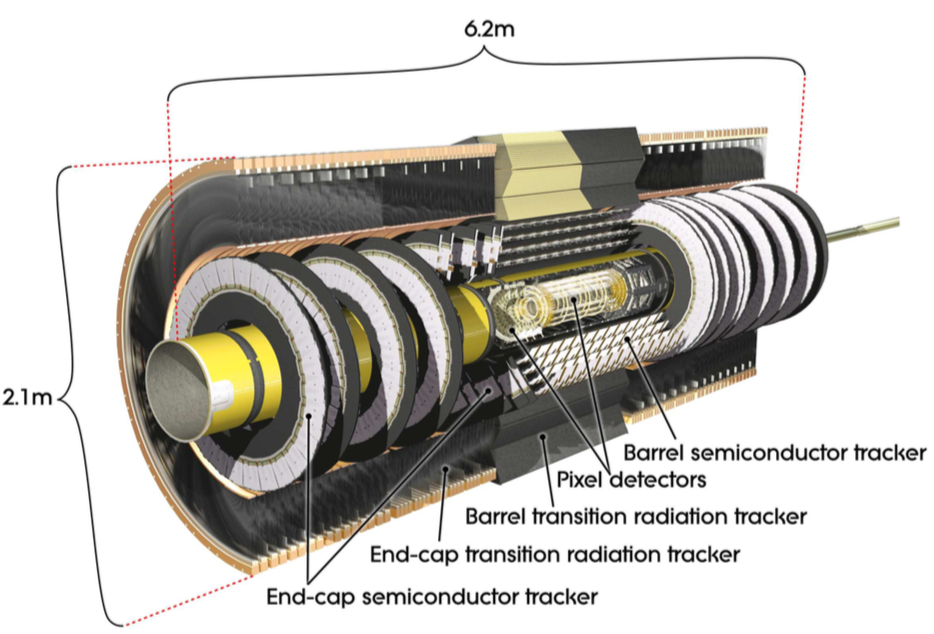
\includegraphics[width=0.75\textwidth]{figures/chapter2/atlas_inner_detector}
        \caption{
            Cross-sectional view of the ATLAS inner detector. Shown are the barrel
            and end-cap portions of the pixel, SCT, and TRT detectors.
        }
        \label{fig:atlas_inner_detector}
    \end{center}
\end{figure}

\begin{figure}[!htb]
    \begin{center}
        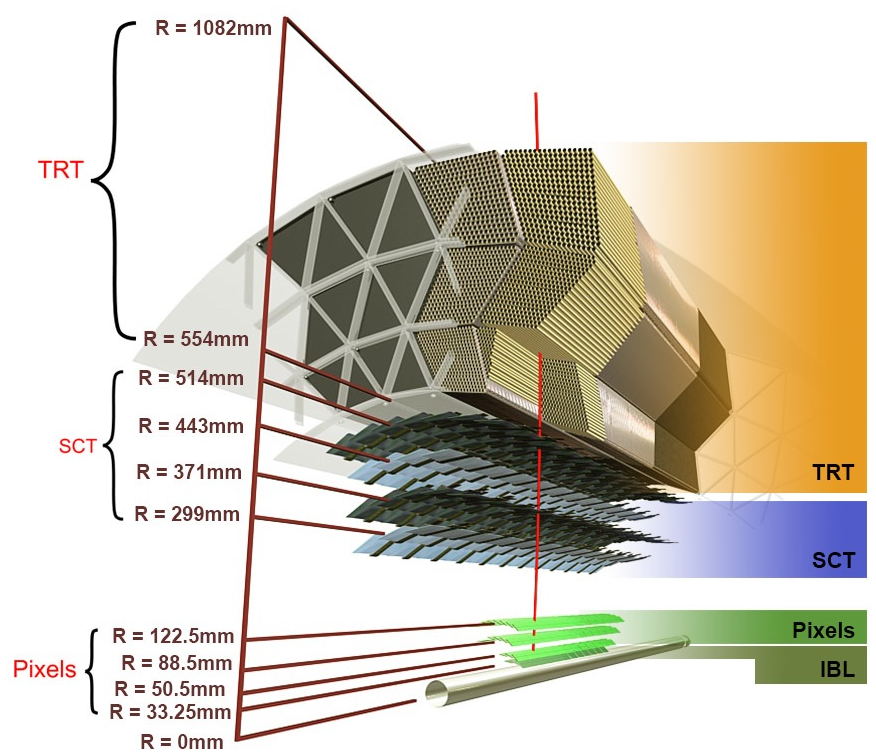
\includegraphics[width=0.6\textwidth]{figures/chapter2/atlas_ID_barrel_exploded}
        \raisebox{1.4cm}{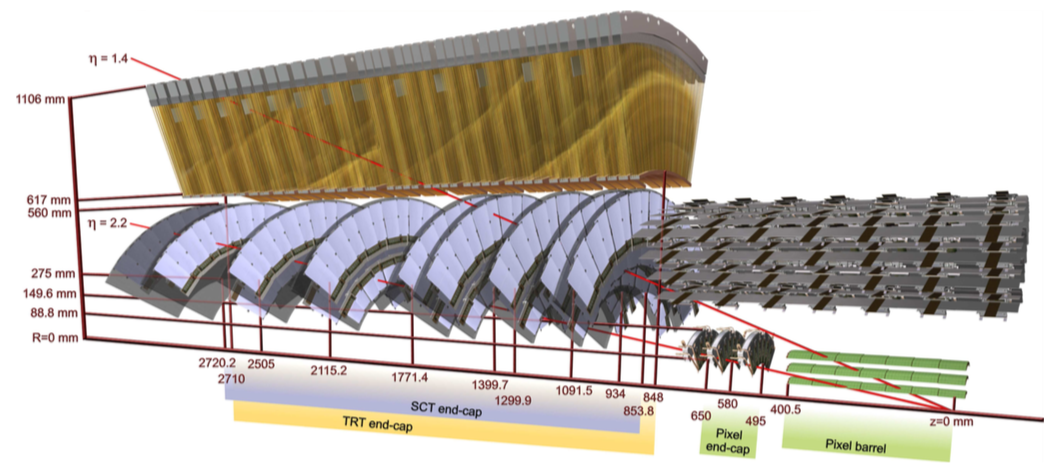
\includegraphics[width=0.85\textwidth]{figures/chapter2/endcap_ID_exploded}}
        \caption{
            Exploded views of the barrel (\textit{left}) and endcap (\textit{right}) portions
            of the inner-detector.
        }
        \label{fig:atlas_ID_exploded}
    \end{center}
\end{figure}

\subsubsection{The Pixel Detector and IBL}
\label{sec:id_pixel}

The pixel detector is the innermost subdetector of the ID, situated very near to and surrounding
the beam-pipe.
It is composed of three separate sections: a barrel section and two end-cap sections.
The barrel section  of the pixel detector has a cylindrical geometry and the end-cap sections
are disks centered on the beam-pipe.
The barrel section has four layers, each with increasing radius, and there are three disks in each
of the end-caps. This ID geometry, shown in Figure~\ref{fig:atlas_ID_exploded}, covers
the region $\lvert \eta \rvert < 2.5$.

The pixel detector, being so near the $pp$ collisions, is subject to the highest particle
fluxes of any other subsystem.
As a result, it is built to have very fine granularity: its sensing elements consist of
$250$\,\micron~thick detectors housing pixels of reverse-biased n-type semiconductor material,
each having a nominal size of $50\times400\,\micron^2$.
In total, there are roughly 80 million channels read out from the pixel detector alone.
This allows for the pixel detector's fine spatial hit resolution of $10\,\micron$ in
$(r-\phi)$ and $115\,\micron$ along $z$.

The innermost layer of the pixel detector's barrel section is referred to as the
\textit{Insertable B-Layer} (IBL), and was installed at the beginning of the Run-II
data-taking period~\cite{Capeans:1291633}.
It corresponds, essentially, to the instrumentation of the ATLAS beam-pipe, as seen in Figure~\ref{fig:pixel_detector_trans},
and is located at a radial distance of 3.3\,cm.
It alone accounts for 8 million readout channels of
the pixel detector --- resulting in an ultra precise spatial hit resolution of $8\,\micron$ in $(r-\phi)$ and
$40\,\micron$ along $z$.
Beyond improving the overall measurements and reconstruction of charged particle tracks,
the IBL was installed in order to improve the performance of secondary vertex
reconstruction --- an essential ingredient to the algorithms associated with
the reconstruction and identification of jets originating from the decays
of $b$-hadrons whose decays occur at radial distances frequently beyond that
of the IBL.



\begin{figure}[!htb]
    \begin{center}
        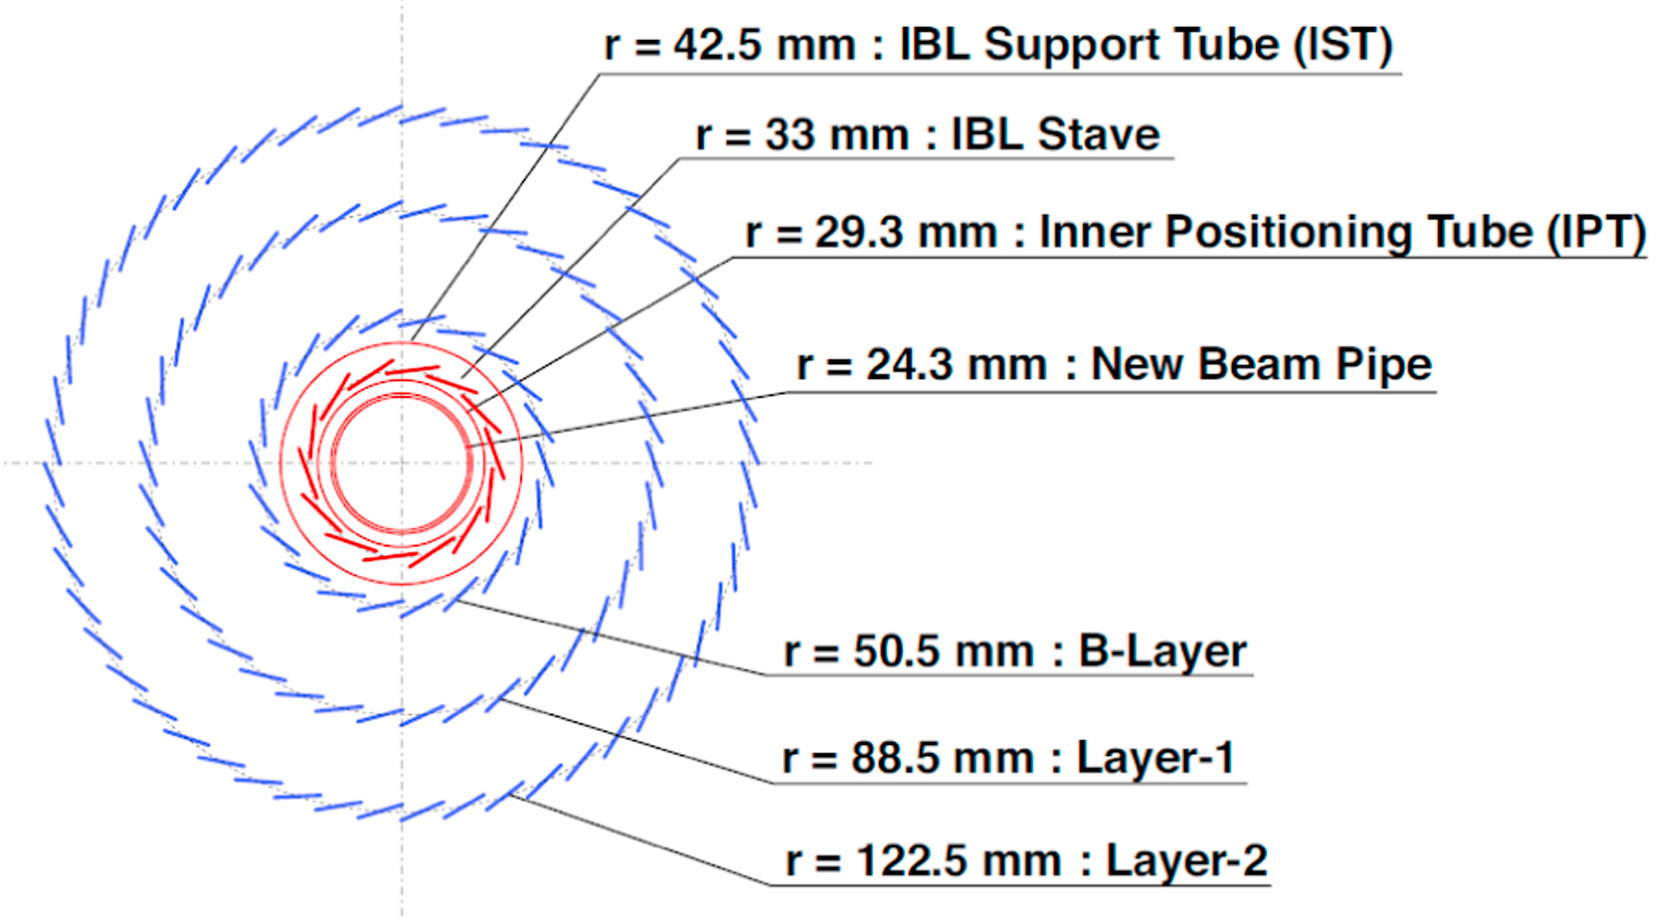
\includegraphics[width=0.8\textwidth]{figures/chapter2/pixel_detector_trans}
        \caption{
            Transverse view of the barrel section of the pixel detector, showing
            the innermost layer, the Insertable B-Layer (IBL) (red), and the
            three surrounding layers (blue). From Ref.~\cite{Backhaus:2016ctq}.
        }
        \label{fig:pixel_detector_trans}
    \end{center}
\end{figure}


%%%%%%%%%%%%%%%%%%%%%%%%%%%%%%%%%%%%%%%%%%%%%%%%%%%%%%%%%%%%%%%%%%%%%
%%%%%%%%%%%%%%%%%%%%%%%%%%%%%%%%%%%%%%%%%%%%%%%%%%%%%%%%%%%%%%%%%%%%%
%
% CALORIMETERS
%
%%%%%%%%%%%%%%%%%%%%%%%%%%%%%%%%%%%%%%%%%%%%%%%%%%%%%%%%%%%%%%%%%%%%%
%%%%%%%%%%%%%%%%%%%%%%%%%%%%%%%%%%%%%%%%%%%%%%%%%%%%%%%%%%%%%%%%%%%%%
\subsection{Calorimeter Systems}
\label{sec:calorimeters}

The ATLAS calorimeter systems are situated outside of the ID and central solenoid and
are tasked with the measurement and containment of showers from electrically charged and neutral particles.
A view of the calorimeter systems is provided by Figure~\ref{fig:atlas_calorimeters_cutaway}.
Broadly speaking, there are two types of calorimeters based on their purpose:
electromagnetic and hadronic calorimeters.
The electromagnetic calorimeter system has $\eta$ coverage that matches the inner-detector
and is optimized for precision measurements of electrons and photons.
The hadronic calorimeter system has readout cells that are generally of
coarser granularity as compared to the electrogmagnetic calorimeter and
is designed to meet the requirements for jet and missing transverse momentum
measurements.
Besides classification by physics purpose, the calorimeter system can also
be broken into two classes based on detector technology: either based
on gaps of cooled liquid-argon~\cite{CERN-LHCC-96-041} or on scintillating tiles as the active media~\cite{CERN-LHCC-96-042}.

\begin{figure}[!htb]
    \begin{center}
        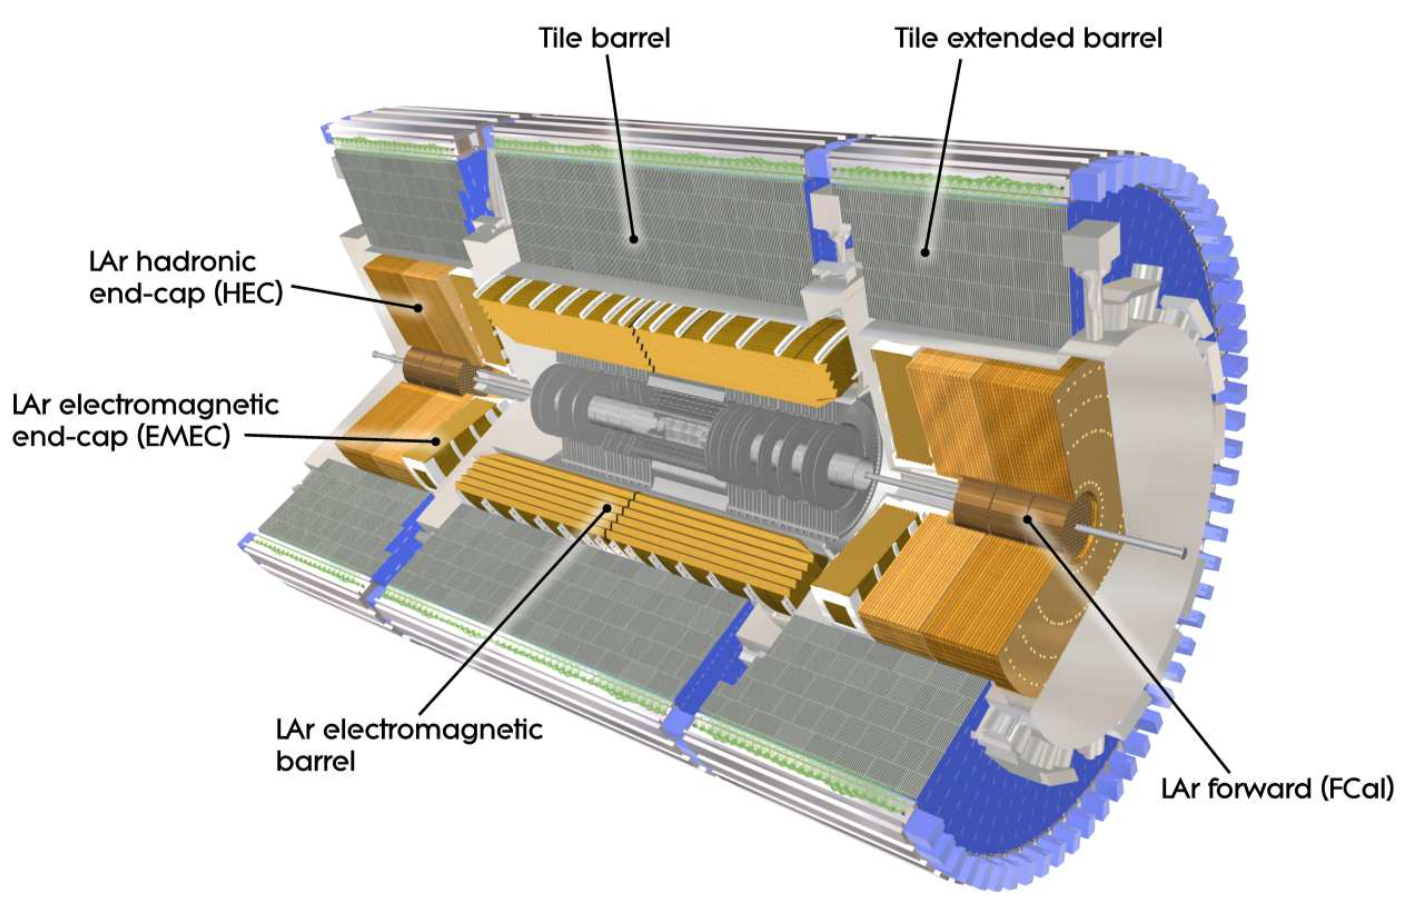
\includegraphics[width=0.9\textwidth]{figures/chapter2/calorimeters/atlas_calorimeter_cutaway}
        \caption{
            Cut-away view of the ATLAS calorimeter system, with liquid-argon and sctintillating-tile
            subsystems indicated.
        }
        \label{fig:atlas_calorimeters_cutaway}
    \end{center}
\end{figure}

\subsubsection{Electromagnetic Calorimeter}
\label{sec:calo_em}

The electromagnetic (EM) calorimeter is a high-granularity lead/liquid-argon (LAr)
sampling calorimeter situated outside of the ID and sharing the
same cryostat as the the central solenoid.
It consists of barrel and end-cap sections that cover the entire
range within $\lvert \eta \rvert < 3.2$ and is illustrated in Figure~\ref{fig:atlas_calorimeters_cutaway}.
The structures of the electromagnetic barrel and end-cap calorimeters
are shown in Figure~\ref{fig:em_calo_section}.
The EM calorimeter is designed in an accordian type structure to provide full coverage
in $\phi$.
The cooled LAr fills the gaps between layers of the
accordian structure.
Passing particles from the interaction point undergo scattering and bremsstrahlung processes as they pass through
the lead absorbers. The resulting electrons and photons ionise the LAr, producing
drift electrons and ions whose signals are read out by the interleaved readout
electrodes. The 2.1\,mm drift gap has an operating voltage of $\approx 2$\,kV.
The electromagnetic calorimeter is $>22$ radiation lengths ($X_0$), ensuring
that the majority of electrons and photons are completely contained within the EM calorimeter.
The majority of the EM energy, amounting to approximately 16\,$X_0$, is contained
within the second sampling layer (see Figure~\ref{fig:em_calo_section}).
The fine granularity of the readout, indicated in Figure~\ref{fig:em_calo_section},
was designed with the ability to distinguish individual photons arising from $\pi^0 \rightarrow \gamma \gamma$
decays. The ability to distinguish photons pairs so precisely is also important for the
main Higgs boson decay channel used for its disovery, $h \rightarrow \gamma \gamma$.

In the region $\lvert \eta \rvert < 1.8$, a so-called \textit{presampler} detector is used to correct
for the energy lost by electrons and photons due to material interactions occuring
upstream of the EM calorimeter.
It is a single LAr layer, with width 1.1\,cm (0.5\,cm) in the barrel (end-cap).

\begin{figure}[!htb]
    \begin{center}
        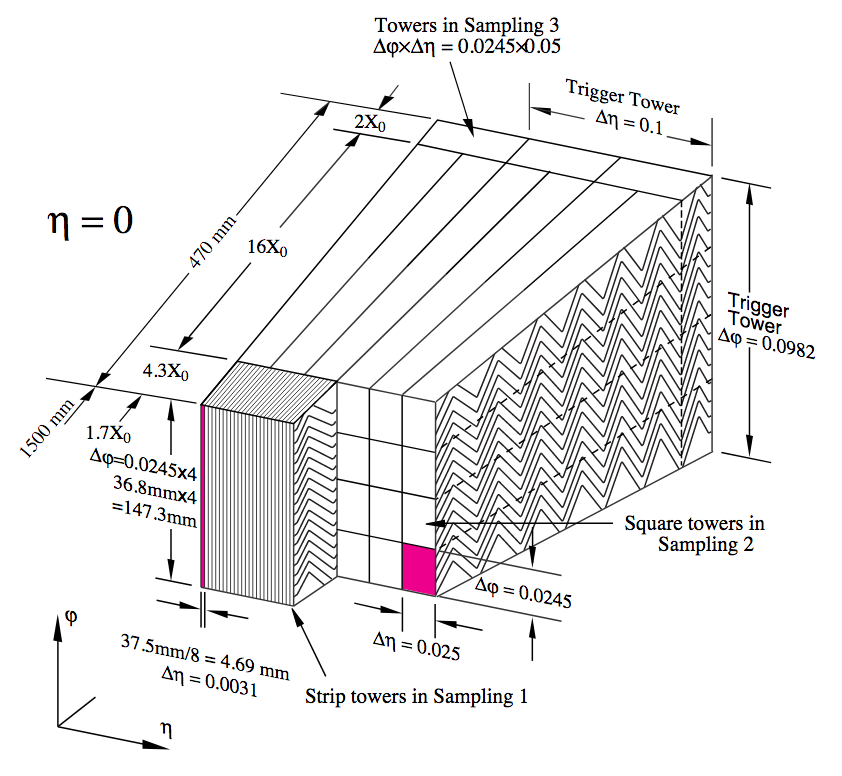
\includegraphics[width=0.6\textwidth]{figures/chapter2/calorimeters/atlas_em_calo_barrel}
        \raisebox{1.5cm}{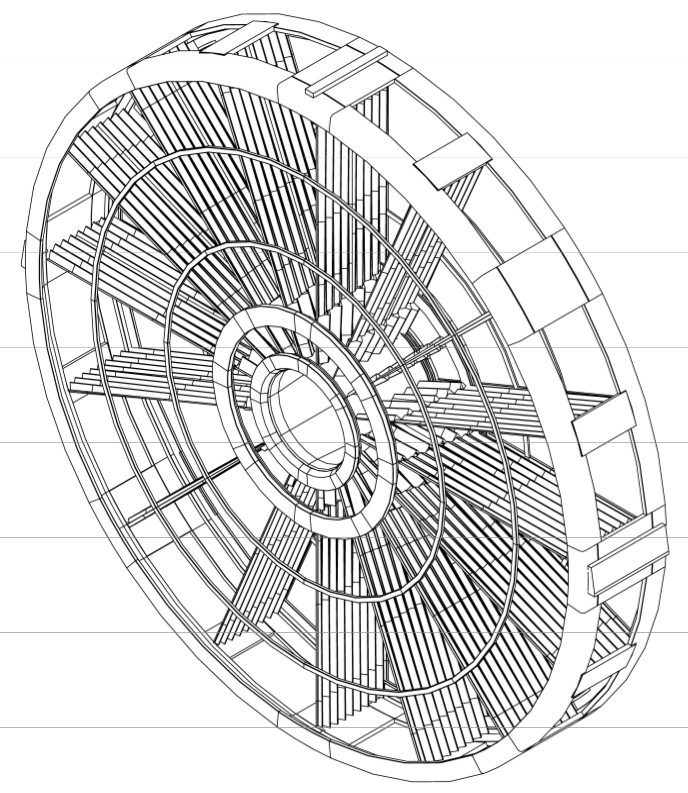
\includegraphics[width=0.3\textwidth]{figures/chapter2/calorimeters/atlas_em_calo_endcap}}
        \caption{
            \textbf{\textit{Left}}: Cut-away view of the barrel electromagnetic calorimeter and its accordian
                structure. Indicated are
                the geometry and absorption properties of the three sampling layers.
                Also indicated is the granularity of the electrode readout in $\Delta \phi \times \Delta \eta$
                in each layer.
            \textbf{\textit{Right}}: Diagram of the electromagnetic end-cap calorimeter accordian wheel structure
                (only a sub-set of the accordian structure is shown).
        }
        \label{fig:em_calo_section}
    \end{center}
\end{figure}

\FloatBarrier
\subsubsection{Hadronic Calorimeter}
\label{sec:calo_had}

The barrel section of the hadronic calorimeter is composed of a
lead/scintillating-tile type detector whereas the end-cap hadronic
calorimeter is based on copper/LAr-based technology.

The lead/scintillating-tile calorimeter (the `tile calorimeter') is located just beyond
the EM calorimeter.
It is composed of a barrel section, covering $\lvert \eta \rvert < 1.0$,
and two extended barrels that cover $0.8 < \lvert \eta \rvert < 1.7$ (see Figure~\ref{fig:atlas_calorimeters_cutaway}).
It is a sampling calorimeter using steel as the passive absorber and scintillating
plastic tiles as the active media.
The tile calorimeter is composed of modules in which the scintillating
tiles are situated in $(r-\phi)$ within the steel absorbers, as shown in Figure~\ref{fig:tile_calo}.
The detector is segmented radially into three layers and the readout of the
scintillation light, using wavelength-shifting fibers that are fed into photomultiplier tubes (PMT)
situated along the outer radii, is organized in a projective
geometry, also illustrated in Figure~\ref{fig:tile_calo}.
In the barrel (extended barrel) section, most of the hadronic energy is captured by the first (last) two
layers which account for $\approx 5.5$ ($6$) hadronic interaction lengths ($\lambda$)
of the $\approx 7$ in total.

The hadronic end-cap (HEC) calorimeter consists of two wheels per end-cap, situated
behind the electromagnetic end-cap calorimeter, and
provides calorimetric coverage in the range $1.5 < \lvert \eta \rvert <3.2$.
A view of the HEC can be seen in Figures~\ref{fig:atlas_calorimeters_cutaway} and \ref{fig:fcal}.
The HEC calorimeter is built from layers of copper plates interleaved with 8.5\,mm LAr gaps
which provide the active medium for this sampling calorimeter.
The readout structure is obtained by dividing the gaps into separate drift zones for
which there are dedicated readout electrodes.
This readout structure is arranged in a projective geometry.

\begin{figure}[!htb]
    \begin{center}
        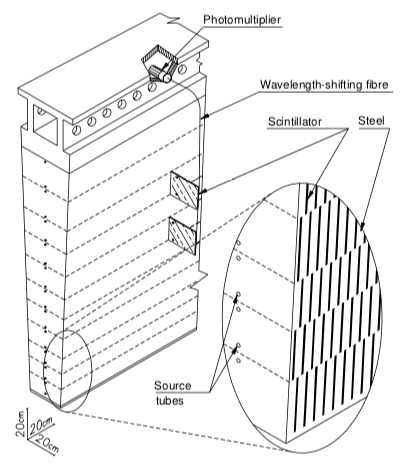
\includegraphics[width=0.4\textwidth]{figures/chapter2/calorimeters/atlas_tile_module}
        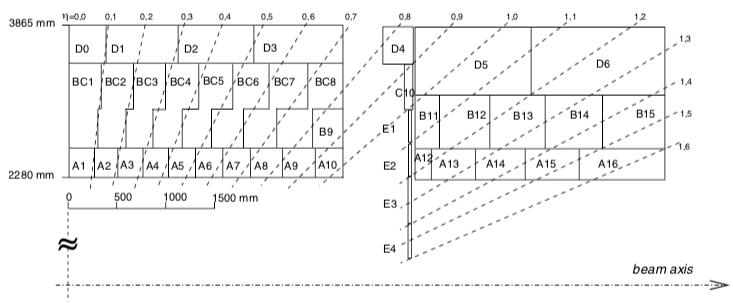
\includegraphics[width=0.9\textwidth]{figures/chapter2/calorimeters/atlas_tile_plan_view}
        \caption{
            \textbf{\textit{Top}}: A view of a tile calorimeter module with its interleaved steel
                absorbers and scintillating tiles and PMT readout. Also indicated are the source tubes
                through which radioactive Cesium (Cs) sources are passed for calibration purposes~\cite{Marjanovic:2018ohl}.
            \textbf{\textit{Bottom}}: Illustration of the segmentation of the projective readout of
                both the barrel and extended barrel tile calorimeter.
        }
        \label{fig:tile_calo}
    \end{center}
\end{figure}

\FloatBarrier
\subsubsection{Forward Calorimeter}
\label{sec:calo_forward}

The forward calorimeter (FCal) system~\cite{Artamonov_2008} provides calorimetric coverage to
high $\lvert \eta \rvert$, between $3.1 < \lvert \eta \rvert < 4.9$,
furthering the hermeticity of the detector.
As indicated in Figure~\ref{fig:fcal}, FCal consists of three layers in the
$z$ direction: an electromagnetic layer (FCal 1) and two hadronic layers (FCal 2 and FCal 3).
All three layers use LAr as the active medium but differ in their passive media.
FCal 1 uses copper for its absorber, chosen for its heat removal properties,
while FCal 2 and FCal 3 use tungsten, chosen to provide high containment and
minimisation of the lateral spread of hadronic showers.
The FCal modules consist of matrices of the passive material with regularly
spaced readout tubes  oriented parallel to the beam-pipe that are filled with the cooled LAr.

\begin{figure}[!htb]
    \begin{center}
        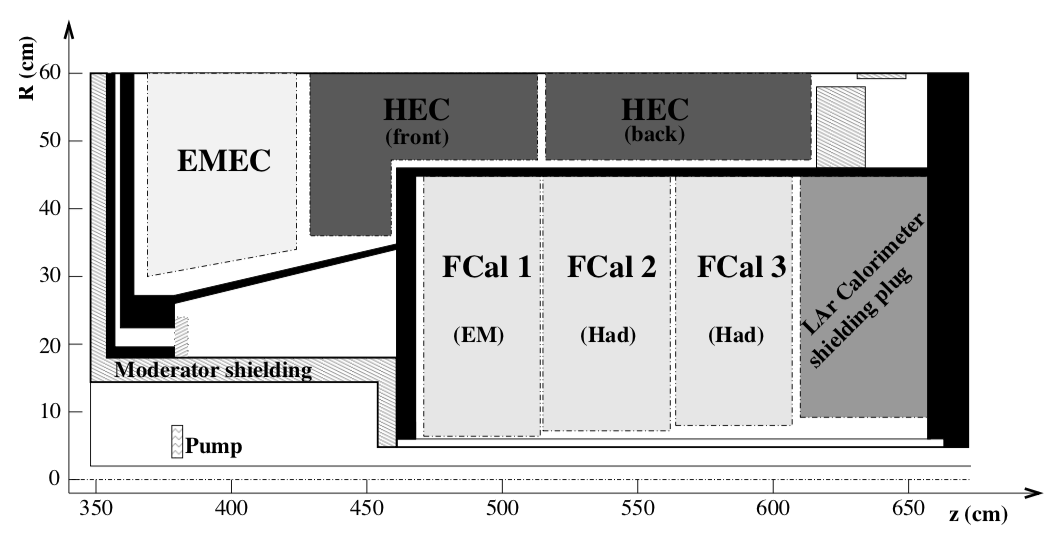
\includegraphics[width=0.65\textwidth]{figures/chapter2/calorimeters/atlas_fcal}
        \caption{
            View of the forward calorimeter (FCal) system. Portions of the electromagnetic
            and hadronic end-cap systems are also shown.
        }
        \label{fig:fcal}
    \end{center}
\end{figure}


%%%%%%%%%%%%%%%%%%%%%%%%%%%%%%%%%%%%%%%%%%%%%%%%%%%%%%%%%%%%%%%%%%%%%
%%%%%%%%%%%%%%%%%%%%%%%%%%%%%%%%%%%%%%%%%%%%%%%%%%%%%%%%%%%%%%%%%%%%%
%
% MUON SPECTROMETER
%
%%%%%%%%%%%%%%%%%%%%%%%%%%%%%%%%%%%%%%%%%%%%%%%%%%%%%%%%%%%%%%%%%%%%%
%%%%%%%%%%%%%%%%%%%%%%%%%%%%%%%%%%%%%%%%%%%%%%%%%%%%%%%%%%%%%%%%%%%%%
\subsection{The Muon Spectrometer}
\label{sec:ms}

Surrounding the calorimeters is the muon spectrometer (MS)~\cite{CERN-LHCC-97-022}, responsible
for the detection of high-momentum, minimum-ionizing muons originating from the $pp$ interaction.
The MS is based on the magnetic deflection of muon tracks, allowing for their
momentum determination.
The bending of the muon trajectories is provided by the large
superconducting air-core toroid magnet system, illustrated in Figure~\ref{fig:atlas_magnet_system},
consisting of a large barrel toroid over the range $\lvert \eta \rvert < 1.4$
and end-cap toroid systems in the range $1.6 < \lvert \eta \rvert < 2.7$.
The superconducting toroid magnet provides an average field of $4\,$T.
The magnetic field bending strength is roughly constant in $\eta$, except in the
region in which the transition between the barrel and end-cap toroids takes place
($1.4 < \lvert \eta \rvert < 1.6$).
A view of the ATLAS detector is shown in Figure~\ref{fig:atlas_in_cavern},
where it can be seen that the volume enclosed by the MS takes up most of the available volume
outside of the calorimeter systems in the underground experimental cavern at Point 1.
It should be noted that the overall design of the superconducting toroid structure,
dictated by the performance requirements of the MS, is what gives ATLAS its large size and essentially
drove the original design of all subdetectors discussed in the previous sections.

There are four types of gaseous radiation detector used in the MS, and their chamber
layout is based on the concept of projective towers.
The chambers follow the structure of the toroid magnet structure and have a 16-fold segmentation
in azimuth, shown in Figure~\ref{fig:muon_segmentation}.
They are arranged in large and small sectors, with the large sectors covering
the regions between the coils of the toroid and the small sectors the azimuthal range
in which the coils sit.
The detector types can be broken into two classes and are either
\textit{precision} or \textit{trigger} chambers.
The precision chambers allow for
the precise measurement the muon tracks as they traverse the MS, specifically the
precise measurement in the bending plane of these tracks so as to allow for accurate
determination of the muon momenta through their curvature.
The trigger chambers have fast signal formation and readout times, allowing for
accurate assignment of a passing muon to a specific $pp$ bunch crossing.
Both types of detectors exist in the barrel and end-cap \textit{stations} of the
MS and there are typically at least three layers of precision-type chambers over the
entire $\lvert \eta \rvert$ range of the MS in order to allow for the sagitta measurement
of the muon tracks necessary for momentum determination.
The layout of these detectors, in both the barrel and end-cap, is shown in
Figure~\ref{fig:muon_plan_view_eta}.

\begin{figure}[!htb]
    \begin{center}
        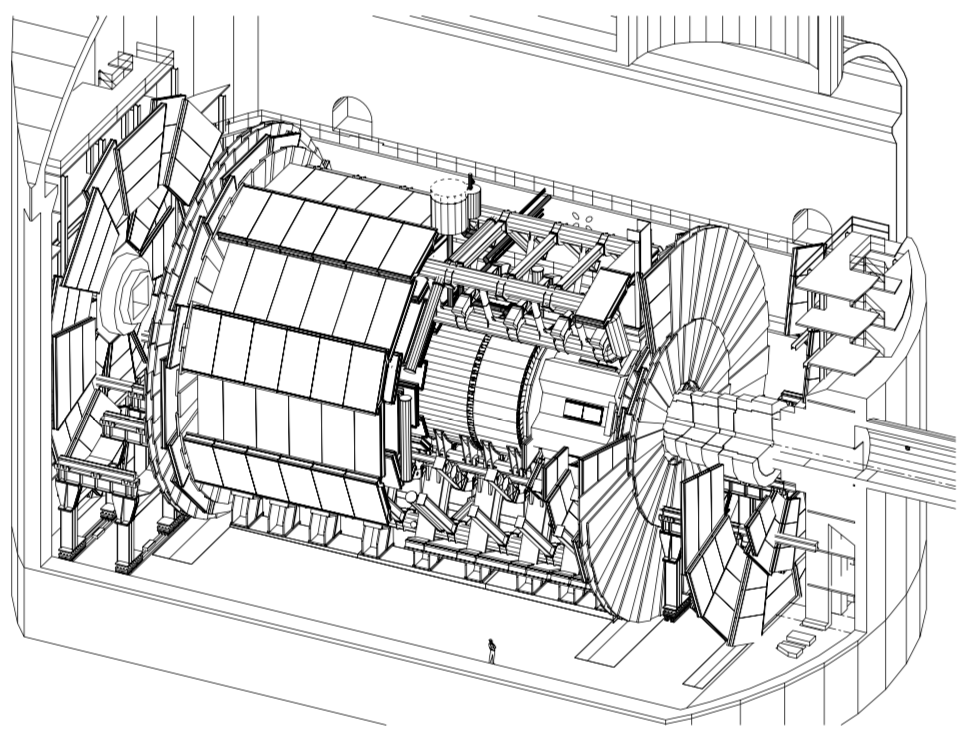
\includegraphics[width=0.8\textwidth]{figures/chapter2/atlas_in_cavern}
        \caption{
            A view of the ATLAS detector inside the underground experimental area
            UX15.
            The cut-away view exposes the toroid structure as well as the
            calorimeter system.
            Notice that the outermost muon stations in the forward regions are located
            at the extreme ends of the cavern.
            {\color{red}{Should move this figure either above or entirely}}
        }
        \label{fig:atlas_in_cavern}
    \end{center}
\end{figure}

\begin{figure}[!htb]
    \begin{center}
        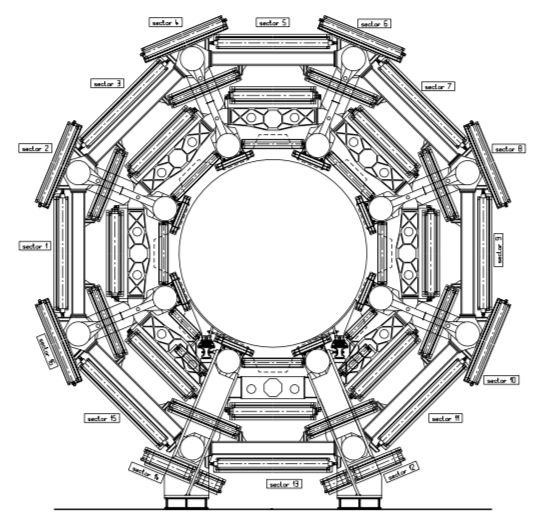
\includegraphics[width=0.4\textwidth]{figures/chapter2/muon_spec/atlas_muon_barrel}
        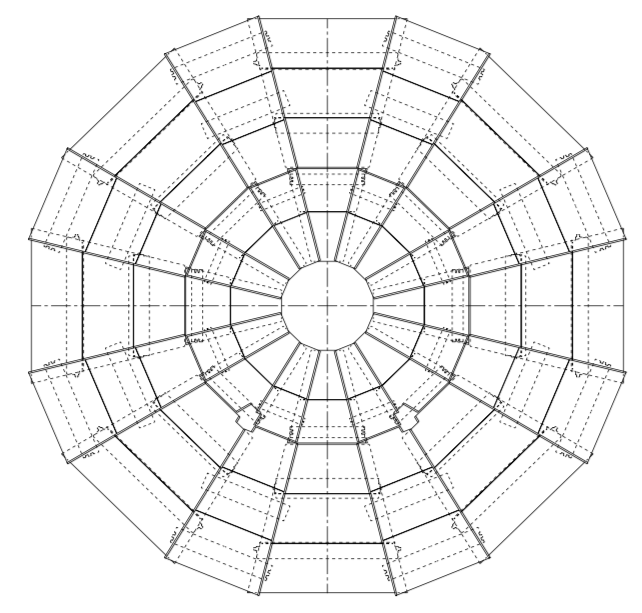
\includegraphics[width=0.35\textwidth]{figures/chapter2/muon_spec/atlas_muon_endcap}
        \caption{
            View of the 16-fold segmentation of the muon spectrometer in the barrel (\textit{left})
            and end-cap (\textit{right}).
            Clearly seen in both is the arrangment of the detector chambers into large and
            small sectors, allowing for complete coverage in azimuth.
            The view of the end-cap is that only of the MDT chambers located at $z\approx13$\,m.
        }
        \label{fig:muon_segmentation}
    \end{center}
\end{figure}

\begin{figure}[!htb]
    \begin{center}
        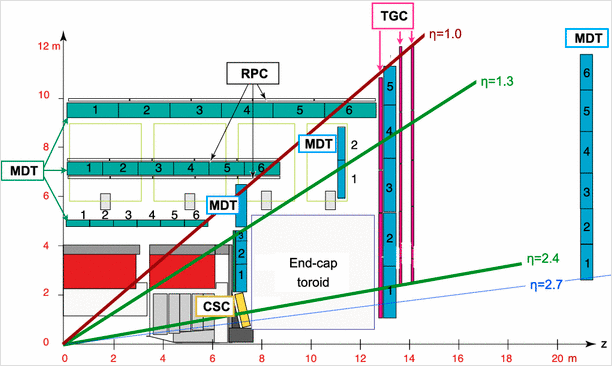
\includegraphics[width=0.8\textwidth]{figures/chapter2/muon_spec/atlas_muon_plan_view_eta}
        \caption{
            A view in the $r-z$ plane of a quadrant of the muon spectrometer (MS).
            Indicated by color are the four detector technologies used in the MS:
            MDT (blue), RPC (grey), TGC (red), and CSC (yellow).
            The light grey boxes at $6 < r < 9$\,m indicate the location of the
            barrel toroid structures.
            Also shown are the envelopes in $\lvert \eta \rvert$ of the barrel,
            small wheel, and big wheel sections of the MS.
        }
        \label{fig:muon_plan_view_eta}
    \end{center}
\end{figure}
\FloatBarrier


\begin{figure}[!htb]
    \begin{center}
        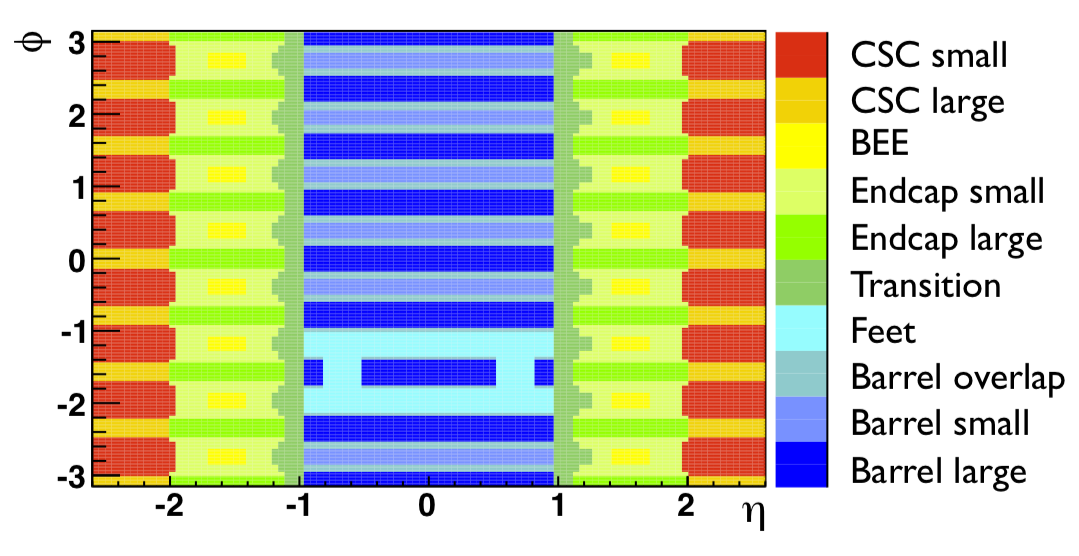
\includegraphics[width=0.7\textwidth]{figures/chapter2/muon_spec/atlas_muon_overlap}
        \caption{
        }
        \label{fig:muon_overlap}
    \end{center}
\end{figure}

\begin{figure}[!htb]
    \begin{center}
        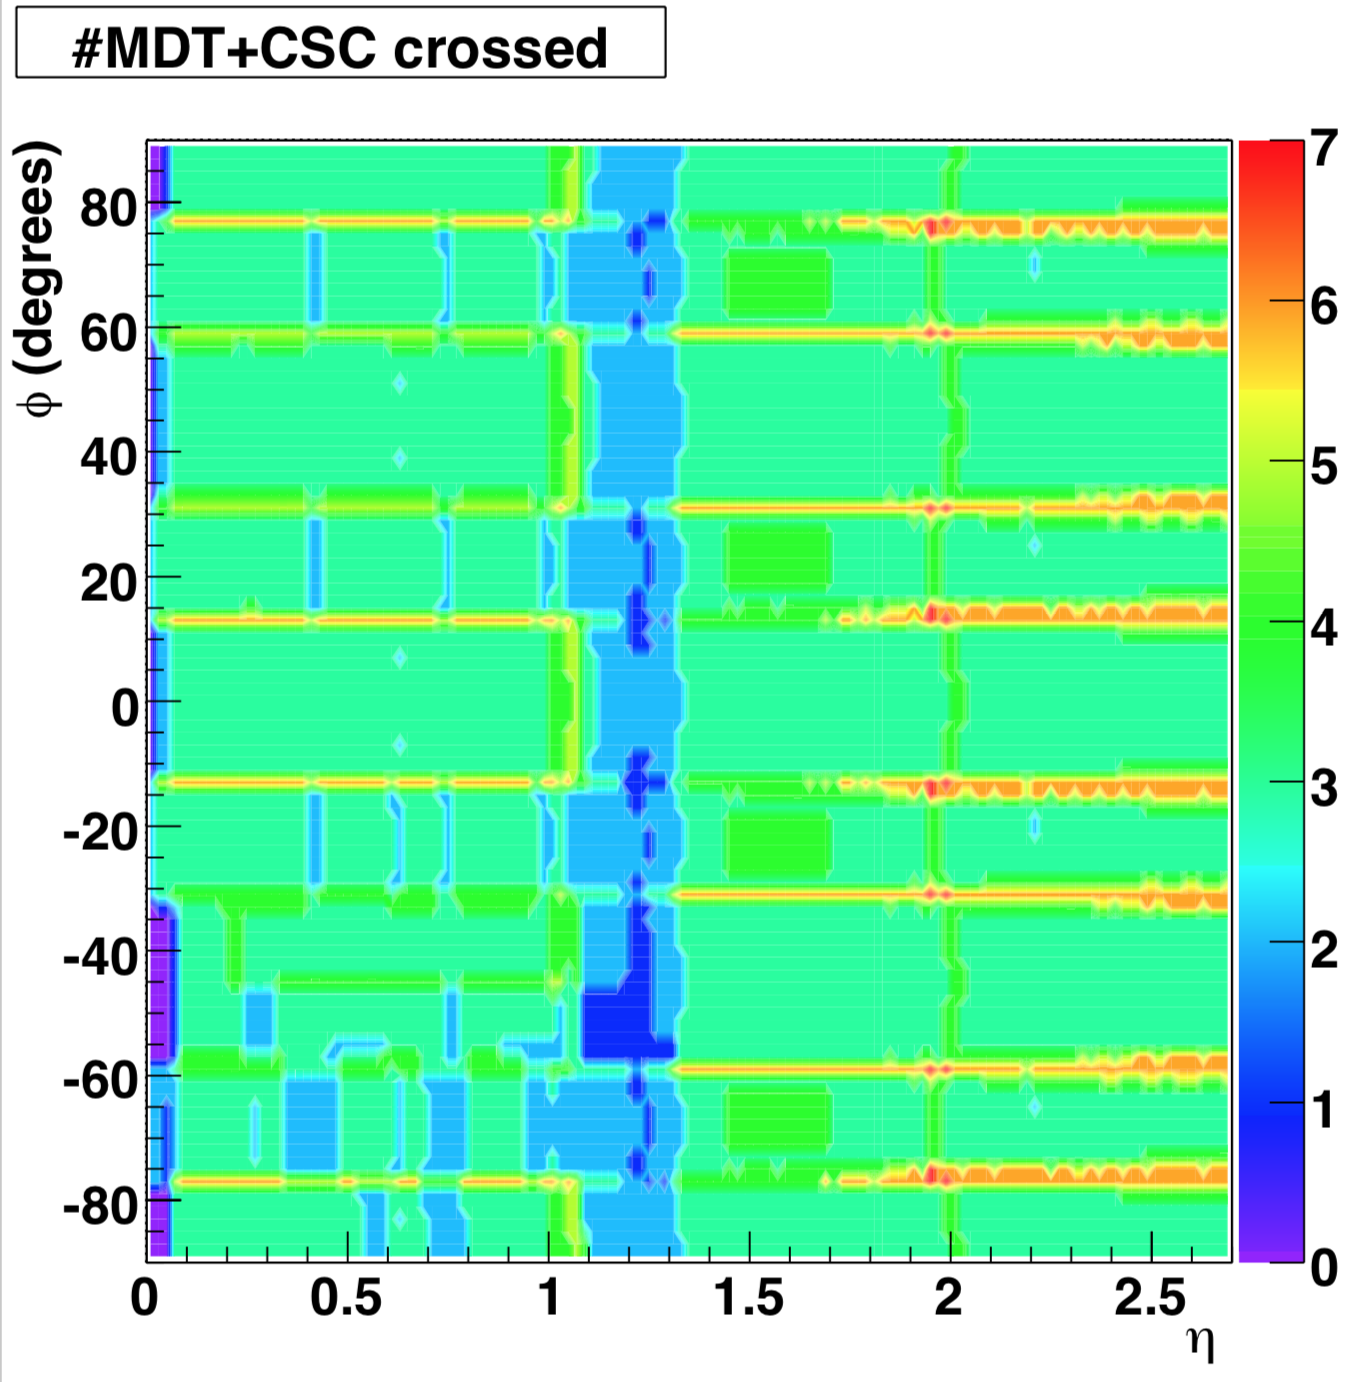
\includegraphics[width=0.7\textwidth]{figures/chapter2/muon_spec/atlas_ms_nchamber_crossed}
        \caption{
        }
        \label{fig:muon_nchambers_crossed}
    \end{center}
\end{figure}


\subsubsection{Precision Muon Chambers}
\label{sec:muon_precision}

\begin{figure}[!htb]
    \begin{center}
        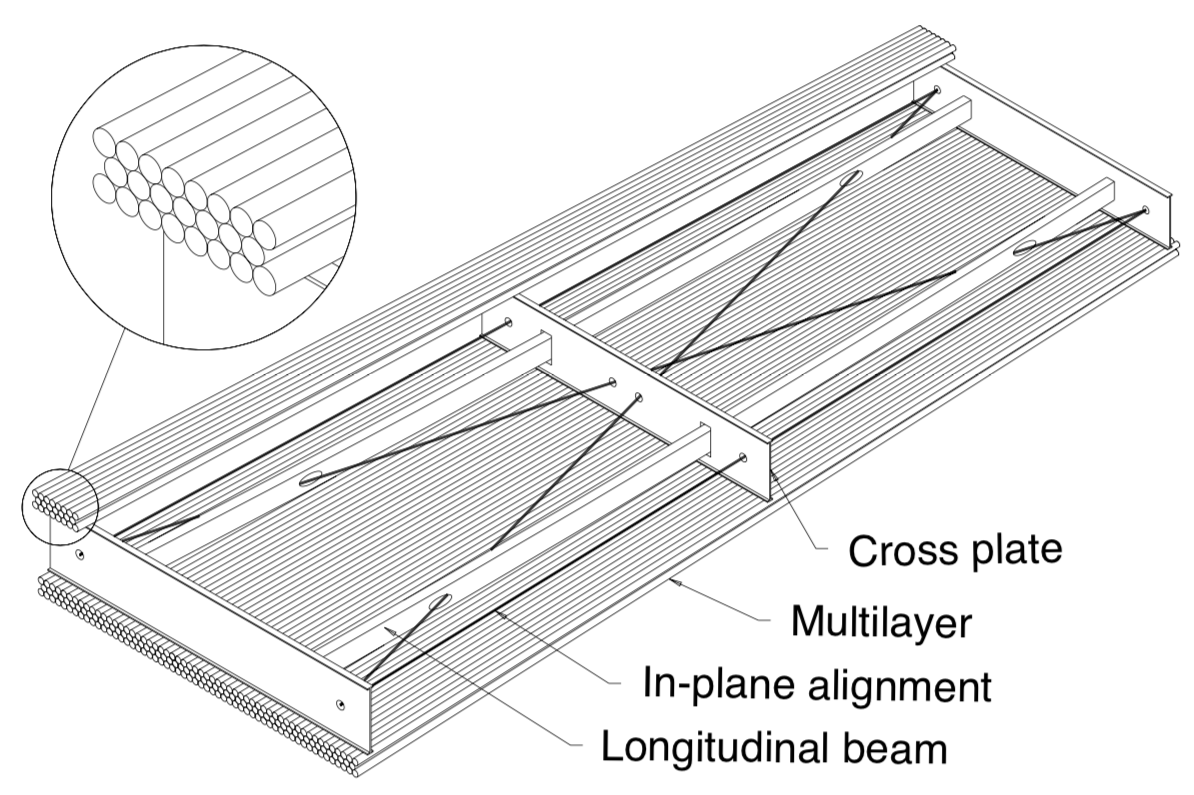
\includegraphics[width=0.5\textwidth]{figures/chapter2/muon_spec/mdt_chamber}
        \raisebox{1.22cm}{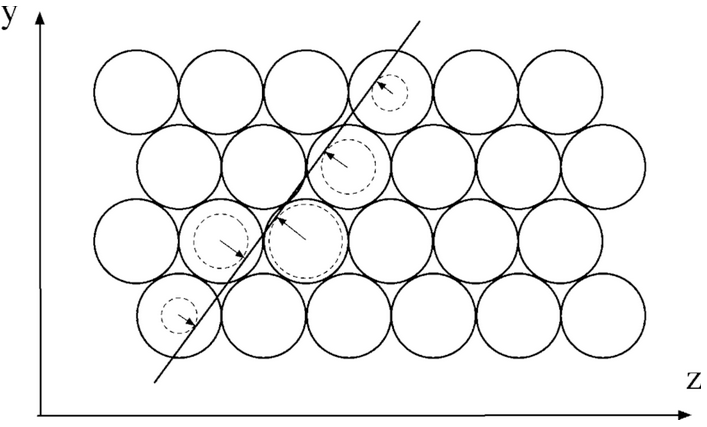
\includegraphics[width=0.32\textwidth]{figures/chapter2/muon_spec/mdt_trackfit}}
        \caption{
            \textit{Left}: Illustration of a double-multilayer MDT chamber with its internal alignment
                and support structure exposed. A zoom-in on the multilayer of MDT tubes is shown.
            \textit{Right}: Illustration of the multilayer MDT tracklet-fitting algorithm~\cite{MDTtrackfit}.
        }
        \label{fig:mdt_chamber}
    \end{center}
\end{figure}

\begin{figure}[!htb]
    \begin{center}
        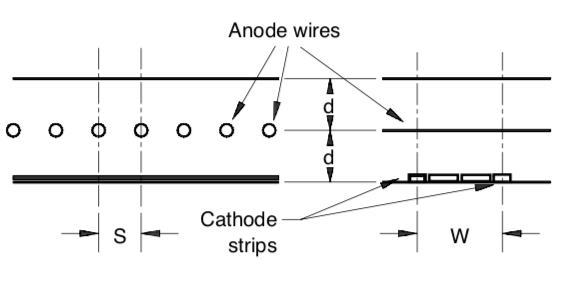
\includegraphics[width=0.55\textwidth]{figures/chapter2/muon_spec/csc_chamber}
        \caption{
            Diagram showing the main components of a cathode-strip chamber (CSC).
            On the \textit{left} (\textit{right}) is a view parallel (perpendicular) to the anode
            wires and perpendicular (parallel) to the cathode strips.
        }
        \label{fig:csc_chamber}
    \end{center}
\end{figure}

\subsubsection{Muon Trigger Chambers}
\label{sec:muon_trigger}

\begin{figure}[!htb]
    \begin{center}
        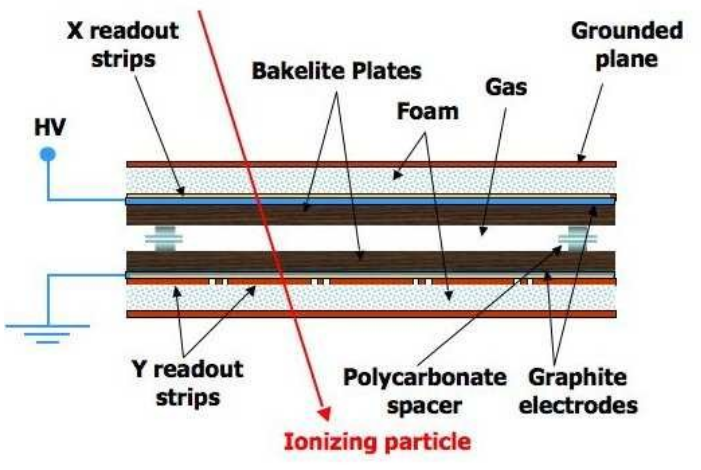
\includegraphics[width=0.5\textwidth]{figures/chapter2/muon_spec/rpc_chamber}
        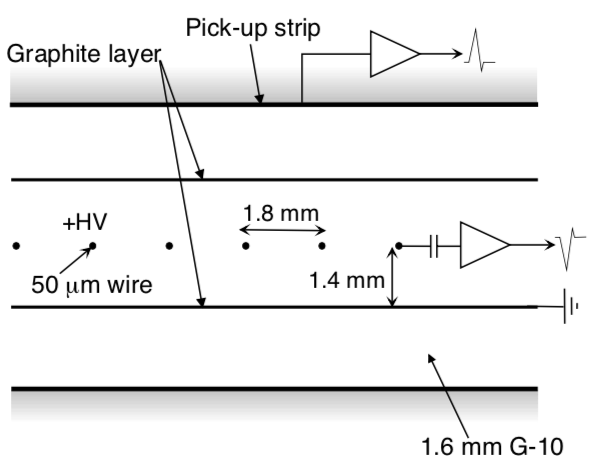
\includegraphics[width=0.38\textwidth]{figures/chapter2/muon_spec/tgc_chamber}
        \caption{
            \textit{Left}: Illustration of a resistive plate chamber (RPC) and its principle of operation.
            \textit{Right}: Diagram showing the main components of a thin-gap chamber (TGC).
        }
        \label{fig:muon_trigger_chamber}
    \end{center}
\end{figure}


%%%%%%%%%%%%%%%%%%%%%%%%%%%%%%%%%%%%%%%%%%%%%%%%%%%%%%%%%%%%%%%%%%%%%
%%%%%%%%%%%%%%%%%%%%%%%%%%%%%%%%%%%%%%%%%%%%%%%%%%%%%%%%%%%%%%%%%%%%%
%
% TDAQ
%
%%%%%%%%%%%%%%%%%%%%%%%%%%%%%%%%%%%%%%%%%%%%%%%%%%%%%%%%%%%%%%%%%%%%%
%%%%%%%%%%%%%%%%%%%%%%%%%%%%%%%%%%%%%%%%%%%%%%%%%%%%%%%%%%%%%%%%%%%%%
\subsection{Trigger and Data Acquisition}
\label{sec:tdaq}

During Run-II operation between 2015--2018, the LHC delivered $pp$ collisions to ATLAS at instantaneous luminosities of
$10^{34}$\,cm$^{-2}$s$^{-1}$, at a bunch spacing of 25\,ns, giving 33.7 $pp$ interactions per bunch crossing on average
(see Figure~\ref{fig:int_lumi_multiyear}).
These values correspond to roughly $10^9$ $pp$ interactions per second.
It is not possible for the ATLAS detector and data storage facilities to both respond to and record every one of these interactions.
In fact, from a physics perspective it is not necssarily desirable to record every single interaction.
The vast majority of such interactions arise from uninteresting, soft collision processes which are not likely
to contain, for example, decays of Higgs bosons or of new particles not accounted for in the SM.
For this reason, the ATLAS detector employs an \textit{online}\footnote{The `online' environment refers to that of the
ATLAS detector during runtime. The `offline' environment refers to anytime in which the data being inspected
or analysed is not \textit{at that time} being recorded by ATLAS but instead has already been stored to permanent storage
and is readily accessible at any time.}
selection strategy to select potentially interesting candidate events to be further processed and considered
for permanent storage. This online selection strategy is referred to as the \textit{trigger} system~\cite{Jenni:616089}.

The ATLAS Run-II trigger system consists of two levels: a hardware-based low-level
trigger, referred to as the \textit{Level-1} (L1) trigger, and a second level software-based high-level trigger (HLT)~\cite{PanduroVazquez:2244345}.
The L1 trigger uses relatively coarse-grained measurements from the calorimeters and MS.
It performs the first level of selection, reducing the initial input 40\,MHz rate of events by
accepting events at a maximal rate of 100\,kHz.
The L1 trigger performs searches for coarse proxies of interesting physics objects: leptons, photons, and jets.
It triggers on electrons and photons based on energy deposits in the EM calorimeter, limited to $\lvert \eta \rvert < 2.5$.
The hadronic calorimeter provides jet candidates to the L1 trigger system via calorimeter `towers' made up of
trigger elements constructed by a sliding window algorithm.
Each trigger element is constructed by calculating energy sums of calorimeter cells in $\eta - \phi$.
Muon-based L1 triggers are based on coincidences of hits along the layers of the MS that form
projective towers, or \textit{roads}, consistent with high-\pT~muons.

The candidate events selected by the L1 trigger system are forwarded to the HLT.
The HLT system is composed of a Level 2 (L2) trigger and the event filter (EF).
The L2 system is similar to the L1 trigger, but performs more refined measurements on the objects and
regions of the detector that resulted in the initial L1 trigger's decision to accept the event.
The EF is purely software based, using the ATLAS Athena reconstruction framework~\cite{AthenaRef}
to perform high level object reconstruction and identification using algorithms similar to those used
in the offline environment ({\color{red}{Section XXX}}).
The HLT accept rate is roughly 1\,kHz.
The accepted events are sent to CERN's permanent storage facilities and are made ready for the offline analysis.
An overview of the trigger system is shown in Figure~\ref{fig:run2_trigger}.


\begin{figure}[!htb]
    \begin{center}
        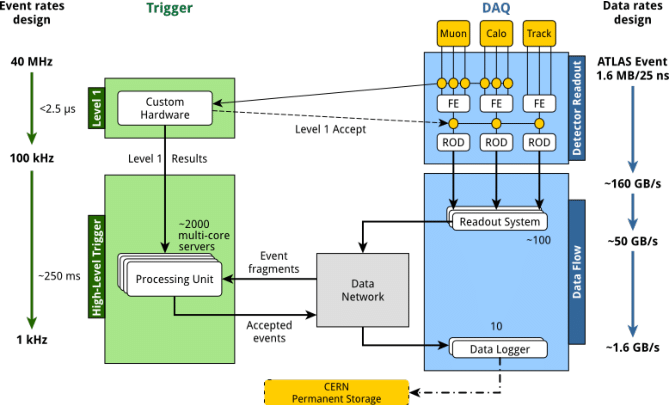
\includegraphics[width=0.7\textwidth]{figures/chapter2/tdaq/atlas_run2_trigger_system}
        \caption{
            Overview of the ATLAS Run-II trigger and data-acquisition architecture.
            Data from the muon and calorimeter systems are used for the Level 1 (L1) trigger, reducing
            the input event rate from 40\,MHz to 100\,kHz.
            The data accepted by the L1 trigger are forwarded to the readout drivers (RODs)~\cite{Jenni:616089}
            which, among other things, re-shuffle the raw data into the standardized ATLAS event format~\cite{Bee:683741}.
            The events selected by the HLT at a rate of 1\,kHz are pulled from the RODs and then forwarded to the permanent
            storage.
            Figure taken from Ref.~\cite{PanduroVazquez:2244345}.
        }
        \label{fig:run2_trigger}
    \end{center}
\end{figure}



% ... and so on

% start START
\setcounter{page}{0}
%\chapter{The Standard Model of Particle Physics}

%\epigraph{\textit{So it goes...}}{---Kurt Vonnegut, \textit{Slaughterhouse
%		Five}}
	
%\epigraph{\textit{Science is a miracle.}}{--Ron Swanson}

\epigraph{\textit{If you wish to make an apple pie from scratch, you must first invent the universe.}}{--Carl Sagan, \textit{Cosmos: A Personal Voyage}}
\epigraph{\textit{All models are wrong, but some are useful.}}{--George Box}


As it stands, what has become known as the `Standard Model (SM) of Particle Physics'
is nothing less than one of the greatest achievments of mankind, due to both
the magnitude by which it has changed our perception of the underlying
nature of the universe and to the clever methods and tinkerings by which this
nature was unveiled by many clever physicists whose history has become veritable lore.
In terms of imagination and insight, it is second only to the special and general theories of relativity --
though the fields are nevertheless intricately intertwined.
%{\color{red}{The latter, though, being put forth by essentially a single person and the latter by a great many...}}.

Not considering the scientific progress made in the $18^{th}$ and $19^{th}$ centuries, and
ignoring the ancient Greeks despite their fabled invention of atomic theory,
the physical insights and major work that led to the current picture of elementary particle
physics described by the SM began with the \textit{annus mirabilis} papers of Albert
Einstein in the year 1905~\cite{einsteinPEE,einsteinSpecial,einsteinEnergyMass}.
In these papers, Einstein was able to shed light on the quantization of electromagnetic
radiation (building off of the seminal work of Max Planck~\cite{planckBlackBody})
and introduce the special theory of relativity.
These works laid the conceptual
and philosophical groundwork for the major breakthroughs in fundamental physics
of $20^{th}$ century physics: from the `old quantum theory' of Bohr and Sommerfeld
in the early 1900's to the equivalent wavefunction and matrix-mechanics formulations
of Schr{\"o}dinger and Heisenberg that
coalesced into `modern' quantum mechanics in the mid-1920's.
The modern approach, non-relativistic at its heart, provided a sufficient mathematical
and interpretable framework in which to work and match predictions to observed phenomena, old
and new. It has for the most part remained unchanged and is the quantum mechanics that is taught to
students at both the undergraduate and graduate level to this very day.
It is the theory that has since revolutionised all aspects of the physical sciences and
technologies that dictate our everyday-lives.
In the mid-1920's, however, despite
large efforts put forth by the forbears of modern quantum mechanics, the quantum-mechanical
world had yet to be made consistent with Einstein's theory of relativity --- a requirement
that must be met for all consistent physical theories of nature.
It was the insight of Paul Dirac who was finally able to successfully
marry the theory of the quantum with that of relativity when he introduced
his relativistic quantum-mechanical treatment of the electron in 1927 and 1928~\cite{diracEquation,Dirac:1927dy}.\footnote{
A complete history of the people and ideas involved in the development of the modern
theory of Quantum Mechanics can be found in references ~\cite{boffiRiseOfQM,historyQM},
and the references therein.
}
This work provided the starting point for a decades-long search of a consistent quantum-mechanical
and relativistic treatment of electrodynamics, known as \textit{quantum electrodynamics} (QED).
The search for QED ended at the end of the 1940's with the groundbreaking work of Dyson, Feynman, Schwinger, and Tomanaga~\cite{qedTomonaga,qedFeynman0,qedFeynman1,qedFeynman2,qedSchwinger0,qedSchwinger1,qedDyson0,qedDyson1} that introduced the covariant and gauge invariant
formulation of QED --- the first such relativistic quantum field theory (QFT).
QED allowed the physcists to make predictions that agreed with observation at unprecedented levels
of accuracy and has since led to the adoption of its language and mathematical toolkit as the
foundational framework in which to construct models that accurately describe nature.\footnote{
	For a complete discussion of the developments leading up to QED, see the fabulous
	book by S. Schweber~\cite{Schweber:1994qa}.	
}
The SM is no less than an ultimate conclusion of these works: a consistent set of relativistic
quantum field theories, using the language developed by Feynman et al.,
that describes essentially all aspects of the known particles and forces that make up the 
observed universe.

%%%%%%%%%%%%%%%%%%%%%%%%%%%%%%%%%%%%%%%%%%%
%%%%%%%%%%%%%%%%%%%%%%%%%%%%%%%%%%%%%%%%%%%
%% sub section describing SM particle content and lagrangian
%%%%%%%%%%%%%%%%%%%%%%%%%%%%%%%%%%%%%%%%%%%
%%%%%%%%%%%%%%%%%%%%%%%%%%%%%%%%%%%%%%%%%%%
\section{Particles and Forces}
\label{sec:sm_description}

There are four known fundamental forces at work in the universe: electromagnetism,
the weak interaction, the strong interaction, and gravity.
Our understanding of the existence of each of these forces
has essentially been arrived at empirically, with physicists following experimental
clues, and their basic behaviors deduced after long trials of effort.
The SM encompasses all of these forces except for gravity, which currently
is only described by the classical (i.e. not quantum) theory of geometrodynamics, or general
relativity.
The gravitational interaction is incredibly weak in comparison to the others, however, and
is not relevant to the types of particle interactions that we are currently
sensitive to in particle physics experiments.
Electromagnetism is by far the most familiar, as it is the force
most commonly experienced and is what is at work in our everyday life (reaction forces between
objects on tables and chairs, friction, wall-plugs, batteries, DNA structure, etc...) and is typically what
students are first presented with in their physics studies.
The weak force is responsible for things like radioactive decay,
which makes possible the process of nuclear $\beta$-decay and the nuclear
fission process that fuels the sun, for example. The strong force is what binds protons
and neutrons together, and thus is responsible for holding together most of the (ordinary) matter
in the universe.\footnote{`Ordinary' to distinguish from dark matter, for example.}

The forces mediate the interactions between the matter particles, which we use to deduce
their presence. The SM predicts fundamental, point-like particles that appear in two
general classes depending on whether they have integral spin ($\mathcal{S} \in [0,1,2,...)$) or half-integral
spin ($\mathcal{S} \in [1/2, 3/2, ...)$); the former are referred to as \textit{bosons} and the
latter as \textit{fermions}.
In the SM, the particles that are responsible for making up matter are all spin-$1/2$ fermions
and are either \textit{leptons} or \textit{quarks}; within each class
there are three generations (or families) that are essentially copies of the first.
The forces in the SM are interpreted as being mediated by spin-$1$ bosons, referred to as the 
\textit{gauge bosons}.
The leptons and quarks all experience the weak force, but only the quarks experience
the strong interaction. All electrically charged particles interact with the electromagnetic
interaction.

The particles of the SM are described as quantum fields whose dynamics are
described by the SM Lagrangian from which the equations of motions can be derived.
The particles, and by extension the SM Lagrangian that describes them, are found to be invariant under transformations of spacetime 
(space translations, rotations, Lorentz boosts) and three internal transformations described by unitary transformations: $\mathcal{P} \times$\SUthree$_C \times $ \SUtwo$_L \times$ \Uone$_{Y}$.
This is illustrated in Figure \ref{fig:sm_forces}. The strong force is described by a
local \SUthree~symmetry that acts only on the particles that have \textit{color charge}.
The term ``color'' arises from the fact that the color charge is found to exist
in three varieties which have been labelled as red (r), blue (b), or green (g), and due
to the fact that ``colorless'' states are formed when all three are combined (r+g+b), just
like with visible light that humans are familiar with, or when states are formed of color-anti-color
pairs (r+$\bar{\text{r}}$). For this reason, the QFT describing the strong force is called
Quantum \textit{Chromo}dynamics (QCD), and is mediated by eight \textit{gluons} (\fieldG).
The particles subject to the weak force are invariant under weak-isospin \SUtwo~transformations,
mediated by the three  \fieldW~bosons (\fieldWone, \fieldWtwo, \fieldWthree).
The \Uone~transformations, mediated by the \fieldB~boson, preserve weak-hypercharge, $Y$.
The \SUtwo~symmetry is respected only by the left-handed chiral
particles (leptons or quarks), with the right-handed chiral particles not participating.
There is additionally a single scalar (i.e. spin-0) field, the Higgs field, that is an \SUtwo~doublet, about which more will be described shortly.
The particle content thus described is presented in detail in Table \ref{tab:sm_content}.
The \SUtwo~left-handed chiral fields appear as doublets and are grouped in
and `up-down' pair (e.g. (\fieldUl, \fieldDl) or (\fieldEl, \fieldNuEl)) whereas the right-handed chiral fields,
living in the singlet representation of \SUtwo, do not (e.g. \fieldUr)). Note
that the SM does not allow for right-handed neutrinos (a term like \fieldNuR~does not appear).

\begin{figure}[!htb]
	\begin{center}
		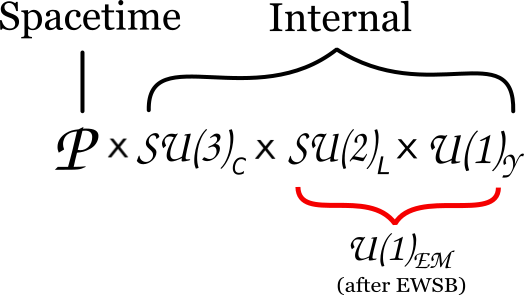
\includegraphics[width=0.5\textwidth]{figures/chapter1/sm_forces}
		\caption{
			The spacetime and internal gauge structure of the SM.
			$\mathcal{P}$ refers to the Poincar{\'e} symmetry group.
			\SUthree$_c$ refers to the \SUthree~symmetry
			of the color sector of QCD and \SUtwo$_{L}\times$\Uone$_{Y}$ refers to the left-handed chiral
			symmetry of the electroweak interaction. After spontaneous symmetry
			breaking due to the Higgs mechanism, the \SUtwo$_L \times$ \Uone$_Y$ symmetry
			reduces to the \Uone$_{EM}$ symmetry of electromagnetism. 
		}
		\label{fig:sm_forces}
	\end{center}
\end{figure}
\FloatBarrier

The SM Lagrangian is shown in Equation \ref{eq:sm_lagrangian} and describes the complete
content of the SM: encompassing all interactions between the known particles and the
symmetries that they obey.

\begin{align}
	\mathcal{L}_{\text{SM}} = -\frac{1}{4} \sum\limits_{\text{gauge}} \mathit{F}_{\mu \nu}^i \mathit{F}^{i\,\mu\nu}
	- \sum\limits_{f} \bar{f}\gamma^{\mu} \mathit{D}_{\mu} f 
	+  (\mathit{D}_{\mu} \phi)^{\dagger} (\mathit{D}^{\mu} \phi) - \mu^2 \phi^{\dagger}\phi - \lambda(\phi^{\dagger}\phi)^2
	\label{eq:sm_lagrangian}
\end{align}
\noindent
The first term of Equation~\ref{eq:sm_lagrangian} is a sum over the three internal gauge groups,  and $\mathit{F}^a_{\mu \nu} = \partial_{\mu} \mathit{A}_{\nu}^a - \partial_{\nu} \mathit{A}_{\mu}^a + g f^{abc} \mathit{A}_{\mu}^{b}\mathit{A}_{\nu}^{c}$, where $\mathit{A}_{\mu}$ is one of the
three gauge fields, $g$ is the associated gauge coupling parameter, and a sum over $i$ is implied. The $f^{abc}$ are the so-called
\textit{structure constants} of the gauge group. For Abelian groups like \Uone, $f^{abc}$ = 0.
For non-Abelian gauge groups like \SUtwo~and \SUthree, $f^{abc} \ne 0$. For example, for
\SUtwo~the structure constants are nothing more than the Levi-Civita totally anti-symmetric tensor, 
$\varepsilon_{ijk}$, giving for the weak gauge force:
\begin{equation}
	\mathbfcal{W}_{\mu \nu} = \partial_{\mu} \mathbfcal{W}_{\nu} - \partial_{\nu} \mathbfcal{W}_{\mu} - g_2 \mathbfcal{W}_{\mu} \times \mathbfcal{W}_{\nu}
\end{equation}
where $\mathbfcal{W}_{\mu}$ is the vector of the three weak gauge fields (\fieldWone, \fieldWtwo, and \fieldWthree) and $g_2$ is their associated gauge coupling. The non-zero $f^{abc}$ of non-Abelian gauge groups means that the gauge bosons of
the weak and strong interactions can interact with themselves due to terms appearing in Equation
\ref{eq:sm_lagrangian} that contain only the gauge bosons. %{\color{red}{add Feynman diagram? -- showing what the squared term of $W_{\mu \nu}$ representing triple and quartic couplings}}

The second term of Equation~\ref{eq:sm_lagrangian} describes the lepton and quark kinetic energies and their interactions with the gauge fields.
The $f$ refer to the fermion fields (quarks and leptons) and the corresponding sum is over all
species of fermion. $\mathit{D}_{\mu}$ is the gauge covariant derivative, and for the SM is
given by:

\begin{equation}
	\mathit{D}_{\mu} = \partial_{\mu} - i g_1 \frac{Y}{2} \mathcal{B}_{\mu} - i g_2 \frac{\tau^i}{2} \mathcal{W}_{\mu}^i - i g_3 \frac{\lambda^a}{2} G_{\mu}^a
	\label{eq:gauge_derivative}
\end{equation}
where $g_1$, $g_2$, and $g_3$ are the gauge coupling constants for \Uone$_{Y}$, \SUtwo$_{L}$, and \SUthree$_{C}$, respectively, that give the overall strength of the associated coupling.
Summation over repeated indices is implied and the $\tau^i$ ($\lambda^a$) are the three (eight)
generators of the \SUtwo~(\SUthree)~gauge group, with $i \in [1,2,3]$ ($a \in [1,..,8]$), and
are typically represented by the Pauli (Gell-Mann) matrices. Note that the form of Equation~\ref{eq:gauge_derivative} is strictly mandated by the requirement that the theory
be \textit{gauge invariant}, i.e. that transformations of the fields under the internal symmetries
of Figure \ref{fig:sm_forces} leave the action of $\mathcal{L}_{\text{SM}}$ unchanged. This is described in detail
in {\color{red}{Appendix XXX}}.

The last three terms in Equation \ref{eq:sm_lagrangian} are all terms including the Higgs field, $\phi$,
and will be discussed in detail in Section~\ref{sec:higgs_description}.

Inspection of Equation~\ref{eq:sm_lagrangian} will reveal two things. The first thing that one
may notice is that it does not appear to describe electromagnetism as it does not have a
term representing the photon, the familiar mediator of the electromagnetic interaction.
The second, and perhaps more immediately obvious, thing is that no mass terms
appear in $\mathcal{L}_{\text{SM}}$: all fields appear to have zero mass! Both of these
facts are counter to our everyday experience: we know electromagnetism is real and that matter,
at the very least, is massive. In the next few sections we will see how these apparent
issues are resolved.


\begin{table}[!htb]
    \caption{
        The particle content of the SM and their transformation
        properties under the SM gauge groups, prior to electroweak symmetry breaking.
        The representations of each of the gauge groups are shown in the three-right
        columns. The \Uone symmetry of weak-hypercharge transformations is one-dimensional
        and the column gives the weak-hypercharge $\mathcal{Y}$ associated with each
        field. For \SUthree and \SUtwo, $\mathbf{1}$ refers to the field belonging to
        the associated singlet representation, $\mathbf{2}$ to the doublet representation,
        $\mathbf{3}$ to the triplet representation, and $\mathbf{8}$ to the octet representation.
    }
    \begin{center}
        \begin{tabularx}{0.96\textwidth}{m{1em} c c c c c c }
        \toprule
        \hline
        & Field Label & Content & Spin & \Uone~($\mathcal{=Y}$) & \SUtwo & \SUthree \\
        \hline
        \rotatebox{90}{\hspace{-0.1cm}\textbf{Quarks} } 
         &   \makecell{\fieldQi \\ \fieldUri \\ \fieldDri} % FIELD
         &   \makecell{ (\fieldUl, \fieldDl), (\fieldCl, \fieldSl), (\fieldTl, \fieldBl) \\ \fieldUr \\ \fieldDr}% CONTENT
         &   \makecell{ $1/2$ \\ $1/2$ \\ $1/2$} % SPIN
         &   \makecell{ $1/6$ \\ $2/3$ \\ $-1/3$}% U(1)
         &   \makecell{ $\mathbf{2}$ \\ $\mathbf{1}$ \\ $\mathbf{1}$}% SU(2)
         &   \makecell{ $\mathbf{3}$ \\ $\mathbf{3}$ \\ $\mathbf{3}$}\\ % SU(3)
        %\cdashline{1-7}
        \rotatebox{90}{\hspace{-0.1cm}\textbf{Leptons} }
         &   \makecell{\fieldLi \\ \fieldEri} % FIELD
         &   \makecell{ (\fieldEl, \fieldNuEl), (\fieldMul, \fieldNuMul), (\fieldTaul, \fieldNuTaul) \\ \fieldEr, \fieldMur, \fieldTaur}% CONTENT
         &   \makecell{ $1/2$ \\ $1/2$ }% SPIN
         &   \makecell{ $1/2$ \\ $-1$ }% U(1)
         &   \makecell{ $\mathbf{2}$ \\ $\mathbf{1}$ }% SU(2)
         &   \makecell{ $\mathbf{1}$ \\ $\mathbf{1}$ } \\ % SU(3)
        \midrule
        \rotatebox{90}{\textbf{\stackanchor{Gauge}{Fields}} }
         &   \makecell{\fieldB \\ \fieldW \\ \fieldG } % FIELD
         &   \makecell{ \fieldB \\ (\fieldWone, \fieldWtwo, \fieldWthree) \\ \fieldG$_a$, $a\in[1,..,8]$ }% CONTENT
         &   \makecell{ $1$ \\ $1$ \\ $1$} % SPIN
         &   \makecell{ $0$ \\ $0$ \\ $0$}% U(1)
         &   \makecell{ $\mathbf{1}$ \\ $\mathbf{3}$ \\ $\mathbf{1}$}% SU(2)
         &   \makecell{ $\mathbf{1}$ \\ $\mathbf{1}$ \\ $\mathbf{8}$}\\ % SU(3)
        \midrule
        \rotatebox{90}{\textbf{\stackanchor{Higgs}{Field}}} 
         &   \makecell{\fieldPhi } % FIELD
         &   \makecell{ (\fieldPhip, \fieldPhizero) }% CONTENT
         &   \makecell{ $0$  } % SPIN
         &   \makecell{ $1/2$  }% U(1)
         &   \makecell{ $\mathbf{2}$ }% SU(2)
         &   \makecell{ $\mathbf{1}$ }\\ % SU(3)
        \hline
        \bottomrule
        \end{tabularx}
    \end{center}
    \label{tab:sm_content}
\end{table}

\FloatBarrier





%%%%%%%%%%%%%%%%%%%%%%%%%%%%%%%%%%%%%%%%%%%
%%%%%%%%%%%%%%%%%%%%%%%%%%%%%%%%%%%%%%%%%%%
%% sub section describing electroweak theory
%%%%%%%%%%%%%%%%%%%%%%%%%%%%%%%%%%%%%%%%%%%
%%%%%%%%%%%%%%%%%%%%%%%%%%%%%%%%%%%%%%%%%%%
\section{The Electroweak Theory}
\label{sec:ewk_description}

It was the work of Glashow, Weinberg, and Salam (GWS) that ultimately put forth a
consistent picture of the chiral weak force and
its unification with electromagnetism~\cite{Glashow:1961tr,Weinberg:1967tq,Salam:1968rm}.
As a result, the theory of particles and fields that respect the \SUewk~gauge
invariance of the SM is sometimes referred to as `GWS theory', 
but is more typically known as the electroweak theory. Since all matter particles
are subject to the electroweak interaction, but only a subset of the particles  that
have color charge (the quarks) are subject to the strong interaction described by QCD, the study of the SM can essentially
be partitioned into two parts: the part that deals with the dynamics and interactions of
colored objects (the `QCD part', $\mathcal{L}_{\text{QCD}}$) and the part that deals with electroweak
interactions, including the Higgs (the `Electroweak part`, $\mathcal{L}_{\text{Electroweak}}$).
Given the broad reach of the electroweak interaction,
in the early days GWS theory was considered the heart of the SM and why
GWS were awarded the Nobel prize in 1979.\footnote{Actually, the acceptance of the GWS theory as the
de-facto SM of the time was not widely held until some years after its publication, when t'Hooft
proved that it was renormalizable~\cite{tHooft:1971akt,tHooft:1971qjg}.
Such a complete understanding in the QCD sector would not come until almost a decade later, in the late
1970's{\color{red}{Woijkec etc CITE}}.}
In this section we will focus on the \SUewk~portion of \SML.

The first thing to remember is that the electroweak theory is \textit{chiral}, i.e., it distinguishes
between left- and right-chiral fermion fields.
For conceptual clarity, it is sometimes useful to take the massless (relativistic) limit of fermions to
get an idea of what chirality represents.
For a massless fermion field, the chirality is equivalent to the perhaps more-famility \textit{helicity},
defined as the projection of its spin onto its momentum (direction of motion).
The helicity of left-handed (right-handed) massless fermions is positive (negative), meaning
that its spin is parallel (anti-parallel) to its momentum.
Fermion fields, then, are commonly defined inclusive of their handedness, with the left-
and right-handed components projected out:
\begin{equation}
	f_{\text{L}} = P_L f = \frac{1}{2}(1- \gamma_5)f, \hspace{0.6cm} f_{\text{R}} = P_R f = \frac{1}{2}(1+\gamma_5)f
	\label{eq:chiral_projection}
\end{equation}

Let's focus only on the first generation of the leptons (the reasoning holds equally well
for the second and third generations, as well as for the quarks). Gathering the
\Uone terms of Eqn.~\ref{eq:sm_lagrangian} , we get Eqn.~\ref{eq:ferm_L_u1},
\begin{align}
    -\mathcal{L}_{\text{ferm}}(\mathcal{U}(1), \text{leptons}) &= \bar{L} i \gamma^{\mu} (i g_1 \frac{Y_L}{2} \mathcal{B}_{\mu})L + \bar{e}_R i \gamma^{\mu} (i g_1 \frac{Y_R}{2} B_{\mu}) e_R \nonumber \\
    &= \frac{g_1}{2} [ Y_L ( \bar{\nu}_L \gamma^{\mu} \nu_L + \bar{e}_L \gamma^{\mu} e_L) + Y_R \bar{e}_R \gamma^{\mu} e_R ] B_{\mu}
    \label{eq:ferm_L_u1}
\end{align}
Where $L = (\nu_L, e_L)$ is used in going from the first to second line. 
%Where we use the fact that $L = (\nu_L, e_L)$ in going from the first to second line of
%Eqn.~\ref{eq:ferm_L_u1}.
Likewise, gathering the associated \SUtwo~terms and noting that $\tau^i W^i$ is a
$2\times2$ matrix (the $\tau^i$ are the Pauli matrices),
%Gathering together the 
%Taking the associated \SUtwo~terms of Eqn.~\ref{eq:sm_lagrangian}, and noting
%that, since the $\tau^i$ are the Pauli matrices, $\tau^i W^i$ is a $2\times2$ matrix, we get:

\begin{equation}
	\begin{multlined}
		\hspace{-2cm}-\mathcal{L}_{\text{ferm}}(\mathcal{SU}(2), \text{leptons}) =  \bar{L}\, i \gamma^{\mu} [i g_2 \frac{\tau^i}{2} W_{\mu}^i ] \,L \\
		= -\frac{g_2}{2} \left[ \bar{\nu}_L \gamma^{\mu} \nu_L W_{\mu}^0 - \sqrt{2}  \bar{\nu}_L \gamma^{\mu} e_L W_{\mu}^+ - \sqrt{2} \bar{e}_L \gamma^{\mu} \nu_L W_{\mu}^- - \bar{e}_L \gamma^{\mu} e_L W_{\mu}^0 \right]
	\end{multlined}
	\label{eq:ferm_L_su2}
\end{equation}
Where we have used the following in Eqn.~\ref{eq:ferm_L_su2},
\begin{equation}
	W_{\mu}^+ = \frac{1}{\sqrt{2}} \left( -W_{\mu}^1 + i W_{\mu}^2 \right) \hspace{1cm} W_{\mu}^- = \frac{1}{\sqrt{2}} \left( -W_{\mu}^1 - i W_{\mu}^2 \right) \hspace{1cm} W_{\mu}^0 = W_{\mu}^3
\end{equation}

%\begin{align}
%	-\mathcal{L}_{\text{ferm}}(\mathcal{SU}(2), \text{leptons}) &= \bar{L} i \gamma^{\mu} [i g_2 \frac{\tau^i}{2} \mathcal{W}_{\mu}^i ] L \notag \\
%	&= -\frac{g_2}{2} (\bar{\nu}_L, \bar{e}_L) \gamma^{\mu} \left( \begin{matrix} \mathcal{W}_{\mu}^3 & \mathcal{W}_{\mu}^1 - i\mathcal{W}_{\mu}^2 \\ \mathcal{W}_{\mu}^1 + i \mathcal{W}_{\mu}^2  & - \mathcal{W}_{\mu}^3\end{matrix} \right) \left( \begin{matrix} \nu_L \\ e_L \end{matrix} \right) \notag \\
%	&= -\frac{g_2}{2} \left[ \bar{\nu}_L \gamma^{\mu} \nu_L \mathcal{W}_{\mu}^0 - \sqrt{2}  \bar{\nu}_L \gamma^{\mu} e_L \mathcal{W}_{\mu}^+ - \sqrt{2} \bar{e}_L \gamma^{\mu} \nu_L \mathcal{W}_{\mu}^- - \bar{e}_L \gamma^{\mu} e_L \mathcal{W}_{\mu}^0 \right]
%\end{align}
%Where Eqn.~\ref{eq:w_redefine} has been used in getting to the last line of Eqn.~\ref{eq:ferm_L_su2}.

Equations~\ref{eq:ferm_L_u1} and \ref{eq:ferm_L_su2} in principle describe all electroweak interactions
between matter and the gauge fields of \SUewk. We would like to make the correspondence
between these equations and what we know to empirically exist: the electromagnetic interaction
and the presence of a massive, charged mediator of the weak nuclear force responsible
for nuclear $\beta$-decay, for example. From the theory of QED, we know that the photon should
couple to charged objects and conserve electric charge. Inspecting all charge-preserving
terms of Eqn.~\ref{eq:ferm_L_u1} and \ref{eq:ferm_L_su2}, we note that we can perform
a field-redefinition,
\begin{equation}
	\left( \begin{matrix} A_{\mu} \\ Z_{\mu} \end{matrix} \right) = \left( \begin{matrix} \cos \theta_W & \sin \theta_W \\ -\sin \theta_W & \cos \theta_W \end{matrix} \right) \left( \begin{matrix} B_{\mu} \\ W_{\mu}^0 \end{matrix} \right)
\end{equation}
where we have used $Y_L = -1$ and introduce,
\begin{equation}
\sin \theta_W = \frac{g_1}{\sqrt{g_1^2 + g_2^2}} \hspace{1cm} \cos \theta_W = \frac{g_2}{\sqrt{g_1^2 + g_2^2}} \hspace{1cm} e = \frac{g_1 g_2}{\sqrt{g_1^2 + g_2^2}}
\label{eq:weinberg_angles}
\end{equation}
The angle $\theta_W$  is known as the \textit{Weinberg angle}. It quantifies the amount of
\textit{gauge mixing} that occurs between the neutral
\SUewk~gauge fields, \fieldB$_{\mu}$ and \fieldWzero$_{\mu}$.

Considering only those terms which are charge-neutral in Eqn.~\ref{eq:ferm_L_u1} and Eqn.~\ref{eq:ferm_L_su2}, one can consider performing a second field-redefinition using
\fieldB~ and \fieldWzero:
\begin{align}
	A_{\mu} &= \frac{g_2 \mathcal{B}_{\mu} - g_1 Y_L \mathcal{W}_{\mu}^0}{\sqrt{g_2^2 + g_1^2 Y_L^2}} \hspace{1cm} Z_{\mu} = \frac{g_1 Y_L \mathcal{B}_{\mu} + g_2 \mathcal{W}_{\mu}^0}{\sqrt{g_2^2 + g_1^2 Y_L^2}} \notag \\
	\hookrightarrow B_{\mu} &= \frac{g_2 A_{\mu} + g_1 Y_L Z_{\mu}}{\sqrt{g_2^2 + g_1^2 Y_L^2}} \hspace{1cm} \mathcal{W}_{\mu}^0 = \frac{-g_1 Y_L A_{\mu} + g_2 Z_{\mu}}{\sqrt{g_2^2 + g_1^2 Y_L^2}}
\end{align}
Using this last result for the re-defined \fieldB~and \fieldWzero~in terms the
fields $A_{\mu}$ and $Z_{\mu}$ to re-write the terms in Eqn.~\ref{eq:ferm_L_u1} and~\ref{eq:ferm_L_su2} involving $\bar{e}_{L,R} \gamma^{\mu} e_{L,R}$, allows
one to see that $A_{\mu}$ should correspond to the photon of electromagnetism if we fix,
\begin{align}
	-e = \frac{g_1 g_2 Y_L} {\sqrt{g_2^2 + g_1^2 Y_L^2}} \hspace{1cm} -e = \frac{g_1 g_2 Y_R}{2 \sqrt{g_2^2 + g_1^2 Y_L^2}} \nonumber
\end{align}
where $e$ is the charge of the positron. Setting $Y_L = -1$ then allows to formulate
the positron charge in terms of the weak couplings $g_1$ and $g_2$ simply as,
\begin{align}
	\label{eq:e_charge_coupling}
	e = \frac{g_1 g_2}{\sqrt{g_1^2 + g_2^2}}
\end{align}
Eqn.~\ref{eq:e_charge_coupling} leads one to introduce the following relations,
\begin{align}
	\sin \theta_W = \frac{g_1}{\sqrt{g_1^2 + g_2^2}} \hspace{1cm} \cos \theta_W = \frac{g_2}{\sqrt{g_1^2 + g_2^2}}
\end{align}
The angle $\theta_W$ is the \textit{Weinberg angle} {\color{red}{What is it's value? -- point to table}}, and it represents the amount of mixing
occuring between the \SUtwo~and \Uone~gauge fields $\mathcal{W}_{\mu}^0$ and $\mathcal{B}_{\mu}$, respectively. Using Eqn.~\ref{eq:e_charge_coupling} gives,
\begin{align}
	g_1 = \frac{e}{\cos \theta_W} \hspace{1cm} g_2 = \frac{e}{\sin \theta_W}
\end{align}
This defines the gauge couplings, $g_1$ and $g_2$, of the electroweak theory purely
in terms of known or measurable quantities.\footnote{We do not describe this in detail, but $\theta_W$
can in principle be determined once the masses of the $\mathcal{W^{\pm}}$ and $\mathcal{Z}$ bosons
are measured.}

From the above algebra, we can re-write the portion of the electroweak Lagrangian describing the
interactions of the first-generation fermions with the electroweak gauge bosons $A_{\mu}$,
$Z_{\mu}$, and $W^{\pm}$ as,
\begin{equation}
\begin{multlined}
\hspace{-0.9cm}\mathcal{L}_{\text{ferm, first-gen.}} = \underbrace{\sum\limits_{f \in \nu_e, e, u, d} e Q_f
\left(\bar{f}\gamma^{\mu} f \right) A_{\mu}}_\text{Neutral, $\sim$ EM}  \\
+ \underbrace{\frac{g_2}{\cos \theta_W} \sum\limits_{f \in \nu_e, e, u, d} \left[ \,\right.\bar{f}_L \gamma^{\mu} f_L
\left( T_f^3 -  Q_f \sin^2 \theta_W \right)
+ \bar{f}_R \gamma^{\mu} f_R \left(-Q_f \sin^2 \theta_W \right) \left. \right]\, Z_{\mu}}_\text{Neutral weak interaction} \\
+ \underbrace{\frac{g_2}{\sqrt{2}} \left[ \right. \left( \bar{u}_L \gamma^{\mu} d_L + \bar{\nu}_{e,L} \gamma^{\mu} e_L \right) \, W_{\mu}^+ + h.c. \left. \right]}_\text{Charged weak interaction}
\end{multlined}
\label{eq:ewk_L_za}
\end{equation}
%$\mathcal{L}_{\text{ferm, first-gen.}} = {\mathop{\sum}_\limits{f}} %_\limits{f \in \nu_e, e, u, d}} e Q_f% \left( %\bar{f}\gamma^{\mu} f \right) A_{\mu} \notag \\
%%	&+ {\mathop{\sum}_\limits{f \in \nu_e, e, u, d}} \frac{g_2}{\cos \theta_W} \left[ \bar{f}_L \gamma^{\mu} f_L \left( T_f^3 - Q_f \sin^2 \theta_W \right) + \bar{f}_R \gamma^{\mu} f_R \left( - Q_f \sin^2 \theta_W \right) \right] Z_{\mu} \label{eq:ewk_L_za} \\
%%	&+ \frac{g_2}{\sqrt{2}} \left[ \left( \bar{u}_L \gamma^{\mu} d_L + \bar{\nu}_L \gamma^{\mu} e_L \right) \mathcal{W}_{\mu}^+ + \text{hermitian conjugate} \right] \notag
%\end{multline}
The related terms for the second and third generations of the fermions,
($\nu_{\mu}, \mu, c, s$) and ($\nu_{\tau}, \tau, t, b$), respectively, are identical.
In Eqn.~\ref{eq:ewk_L_za}, $T_f^3$ ($Q_f$) is the third component of the weak-isospin (electric charge)
of the fermion species $f$. These last terms are related via the Gell-Mann-Nishijima relation,
\begin{align}
	Q_f = T_f^3 + \frac{1}{2}Y
	\label{eq:gell_mann_nishijima}
\end{align}
which can be deduced by following the algebra above, and our having fixed $Y_L = -1$ for
the $(\nu_L, e_L)$ \SUtwo~doublet.

Note that the terms involving \fieldWpm~in Eqn.~\ref{eq:ewk_L_za} are of the form $\bar{\nu}_L \gamma^{\mu} e_L$
which, given the chiral projects of Eqn.~\ref{eq:chiral_projection}, can be
re-written as follows,
\begin{align}
	\bar{\nu}_L \gamma{\mu} e_L = \frac{1}{2} \bar{\nu} \gamma^{\mu}(1-\gamma_5) e
	\label{eq:v_minus_a}
\end{align}
which shows that the charged weak interactions involving \fieldWpm~are the coherent
sum of vector ($\gamma^{\mu}$) and axial-vector ($\gamma^{\mu}\gamma_5$) bilinear covariants; this is the famous
\textit{V-A} charged-current interaction of Fermi's nuclear $\beta$-decay.
It is this \textit{V-A} form that results in the charged interactions of the weak force
not being invariant under chiral transformations ($f_R \leftrightarrow f_L$): it only involves
the left-chiral fermion fields. For this reason, \textit{parity}
is said to be maximally violated by the weak interaction.
This result, as presented in the above, is due to our having injected
it into our assumption on the field content in the first place out of hindsight. There
is no first-principles reason why the weak interactions should be this way, however,
and it was historically arrived at empirically.

What we have shown in this section is that, due to mixing of the SM \SUtwo$_L$
and \Uone$_Y$ gauge fields, we can arrive at an electroweak theory that supports
the known fact that their exists an electromagnetic force that is mediated
by a neutral boson $A_{\mu}$ (the photon) that couples to electrically charged fields: this is what
is shown in the first line of Eqn.~\ref{eq:ewk_L_za}. The field re-definitions described above
also introduce the \fieldWpm~boson as the mediators of the charged electroweak interaction,
responsible for radioactivity, and an additional neutral electroweak interaction mediated
by the \fieldZ~boson.
The fact that the \SUtwo$_L$ and \Uone$_Y$ gauge fields mix, by an amount dictated by $\theta_W$,
suggest that the weak and electromagnetic interactions can be unified into the single
electroweak interaction, as mentioned at the beginning of this section. Later on, we will see
that (gauge) unification such as this plays a large role in our current understanding
of how the universe works.

We have thus shown that the SM predicts the existence of the familiar electromagnetic force,
which is not immediately apparent based on \SML~of Eqn.~\ref{eq:sm_lagrangian}. 
%However, 
%neither the fermions nor the \fieldWpm~or \fieldZ~ appear to have mass -- they still
%have no mass terms appearing in their respective sectors of \SML.
However, it is still not evident how it can
support the experimental fact that fermions have mass and that the mediators of the
weak-nuclear force (the \fieldWpm) \textit{must} be massive given the very short
range of the interaction, a fact known
even before the formulation of QED. No such mass terms
have been provided for in the SM Lagrangian described by Eqn.~\ref{eq:sm_lagrangian}. To resolve this, we need the Higgs mechanism.


%%%%%%%%%%%%%%%%%%%%%%%%%%%%%%%%%%%%%%%%%%%
%%%%%%%%%%%%%%%%%%%%%%%%%%%%%%%%%%%%%%%%%%%
%% sub section describing the higgs mechanism
%%%%%%%%%%%%%%%%%%%%%%%%%%%%%%%%%%%%%%%%%%%
%%%%%%%%%%%%%%%%%%%%%%%%%%%%%%%%%%%%%%%%%%%
\section{The Higgs Mechanism and Electroweak Symmetry Breaking}
\label{sec:higgs_description}

The missing mass-terms for the fields in \SML~are provided by the
Brout-Englert-Higgs (BEH) mechanism~\cite{Englert:1964et,Higgs:1964ia,Higgs:1964pj}.
Before describing the specifics of the BEH mechanism, we should first describe the problem
of why \SML~doesn't support general mass terms for any of the fields in the first place.
That is, for example, why can't a fermion term like $m \bar{f} f$ exist in \SML?

Adding mass terms to \SML~for the fermions explicitly breaks the underlying \SUtwo~
gauge symmetry. This can be understood if we recognize the experimentally supported
fact that the left-handed fermions appear as \SUtwo~doublets and that the
right-handed fermions as singlets,
\begin{align}
	m\bar{f}f &= m \bar{f}(P_L + P_R)f \notag \\
				   &= m \bar{f} P_L P_L f + m \bar{f} P_R P_R f  	\label{eq:bad_fermion_mass_term}\\
				   &= m \left( \bar{f}_R f_L + \bar{f}_L f_R \right), \notag
\end{align}
where we have used identity relations of the projection operators $P_L$ and $P_R$ and the fact that $\bar{f}P_L = \bar{f}_R$ (and vice-versa). The last line of Equation~\ref{eq:bad_fermion_mass_term} involve terms
mixing \SUtwo~doublets with \SUtwo~singlets. Such a term is therefore not allowed if we wish to keep the \SUtwo~gauge symmetry intact.

Mass terms for the gauge bosons, of the form $m B_{\mu} B^{\mu}$, also do not work. For the Abelian \Uone~symmetry, for example, gauge invariance implies invariance of \SML~under transformations
of the form $B_{\mu}^{\prime} \rightarrow B_{\mu} - \partial_{\mu}\chi /g$. Such a mass term for
the gauge bosons is clearly not invariant under such a transformation. Even forgoing this fact,
adding such a term would quickly lead to non-renormalizable divergences appearing in the theory,
due to the longitudinal field components that appear in massive field propagators, rendering \SML~meaningless.

The BEH mechanism provides a way out of this problem. It refers to the introduction of a
spin-0 field, the Higgs field (Table \ref{tab:sm_content}), to the SM along with its corresponding interaction
terms to \SML: the last three terms of Equation~\ref{eq:sm_lagrangian}. The final two terms make up
what is referred to as the Higgs potential and can be expressed as,
\begin{align}
	V(\phi) = - \mu^2 \phi^2 - \lambda \phi^4
	\label{eq:higgs_potential}
\end{align}
The Higgs field is an \SUtwo~doublet and it can be seen that the interactions
described by Equation~\ref{eq:higgs_potential} respect \SUtwo~gauge symmetry.
If $\mu^2>0$, nothing all too interesting occurs and Equation~\ref{eq:higgs_potential} describes
a self-interacting, complex scalar field. If we take $\mu^2<0$, however, then the classical
potential described by Equation~\ref{eq:higgs_potential} has non-zero minima located at
$\phi = \pm v$ with $v = \sqrt{-\mu^2 / \lambda}$.
This is illustrated in Figure~\ref{fig:higgs_ewsb}. We see that the stable equilibrium point $\phi_0$
of the Higgs potential, the \textit{Higgs vacuum expectatin value} (vev), is not at $\phi = 0$
but at $v$,
\begin{align}
	\phi_0 = \frac{1}{\sqrt{2}} \left( \begin{matrix} 0 \\ v \end{matrix} \right)
	\label{eq:higgs_vev}
\end{align}
The choice of Equation~\ref{eq:higgs_vev} to represent the Higgs vacuum is motivated by
the requirement that the vacuum not be electrically charged --- a fact motivated very much
by experiment and everyday experience --- so the up-type \SUtwo~component of the Higgs field, $\phi^+$ (Table \ref{tab:sm_content}), is chosen to be zero for $\phi_0$. The choice of an
electrically neutral vacuum sets the rest of the \SUewk~structure of the complex Higgs field
since, by the Gell-Mann-Nishijima relation (Equation~\ref{eq:gell_mann_nishijima}) and charge
conservation,
a  neutral \SUewk~field should have down-type \SUtwo~quantum numbers and \Uone~hypercharge
$Y=1$,
\begin{align}
	Q = T_3 + \frac{1}{2}Y \rightarrow Q_{\phi_0} = -\frac{1}{2} + \frac{1}{2} \times 1 = 0.
	\label{eq:higgs_charge}
\end{align}

Note that Equation~\ref{eq:higgs_vev} states that only one component of the Higgs \SUtwo~doublet
attains a non-zero vev. This clearly means that the \SUtwo~gauge symmetry is not respected
by the choice of $\mu^2 < 0$ and that the electroweak \SUewk~symmetry is
\textit{spontaneously broken}.\footnote{A symmetry of a Lagrangian is said to be
	`spontaneously' broken if the Lagrangian of the underlying theory
	respects the symmetry but it gets broken through dynamical means or if the lowest-energy
	state (vacuum) does not respect the symmetry.
} The Higgs field
acquiring a non-zero vev is then referred to as the \textit{electroweak symmetry breaking} (EWSB) of the SM.

To further examine the physical consequences of EWSB,
we perturb the Higgs field about its minimum value,
\begin{align}
	\phi(x) \propto \left( \begin{matrix} 0 \\ \frac{1}{2}(v + h(x)) \end{matrix} \right),
	\label{eq:higgs_perturb}
\end{align}
where $h(x)$ correspond to excitations of the Higgs field that represent the physically observable
Higgs boson.
Inserting Equation~\ref{eq:higgs_perturb} into the $\mathit{D}_{\mu}\phi$ terms
of Equation~\ref{eq:sm_lagrangian}, one eventually works through the algebra and obtains,
\begin{align}
	\lvert\mathit{D}_{\mu} \phi(x)\rvert^2 = \frac{1}{8} v^2 g_2^2 \left[ \left( W^1_{\mu} \right)^2 +\left( W^2_{\mu} \right)^2 \right] 
		+ \frac{1}{8} v^2 \left( g_1 B_{\mu} - g_2 W_{\mu}^3 \right)^2.
	\label{eq:higgs_gauge_expand} 
\end{align}
Using the field re-definitions for the $W_{\mu}$, $A_{\mu}$ and $Z_{\mu}$ introduced in Section~\ref{sec:ewk_description}, we see that this can be re-written as (modulo factors of 2),
\begin{align}
	\lvert\mathit{D}_{\mu} \phi(x)\rvert^2 \propto \left(\frac{1}{2} v g_2 \right)^2 W_{\mu}^+ W^{-\,\mu} + \left( \frac{1}{2}v \sqrt{g_1^2 + g_2^2} \right)^2 Z_{\mu} Z^{\mu} + (0)^2 A_{\mu} A^{\mu},
	\label{eq:higgs_gauge_masses}
\end{align}
which provide, clearly, mass terms for the electroweak gauge bosons:
\begin{align}
	M_W = \frac{1}{2}v g_2, \hspace{1cm} M_Z = \frac{1}{2}v\sqrt{g_1^2 + g_2^2}, \hspace{1cm} M_A = 0.
	\label{eq:gauge_boson_masses}
\end{align}


The expression for the masses acquired by the \fieldWpm~and \fieldZ~gauge bosons in Equation~\ref{eq:gauge_boson_masses} is expected by Goldstone's theorem~\cite{Goldstone:1962es} which
states that for every broken continuous symmetry one expects an associated massless
scalar field (a `Goldstone boson') to appear in the theory. The fact that the \fieldWpm~and \fieldZ~acquire
mass after EWSB is then interpreted as these fields having acquired longitudinal field
components by `eating' the Goldstone boson degrees of freedom associated with the
breaking of \SUtwo$_L$. The BEH mechanism refers specifically to this means of the gauge
bosons acquiring mass via `eating' the Goldstone bosons.

The fact that the Higgs vev respects charge conservation (Equation~\ref{eq:higgs_charge}) means
that \SML, after EWSB, still respects a local \Uone~gauge symmetry; although now
this is the \Uone~gauge symmetry associated with electromagnetism, \Uone$_{EM}$,
as opposed to that of weak-hypercharge, \Uone$_Y$. This indicated in Figure~\ref{fig:sm_forces}.

There are also additional terms involving the now-massive \fieldWpm~and \fieldZ~ bosons and $h(x)$ in the expansion of $\lvert D_{\mu}\phi(x)\rvert^2$ of
Equation~\ref{eq:higgs_gauge_expand} (not shown) that describe the gauge bosons' interactions with the observable Higgs boson,
involving terms of the form $hVV$ and $hhVV$ ($V\in(W,Z)$) whose coupling strengths depend
on the gauge boson masses (Equation~\ref{eq:gauge_boson_masses}):
\begin{align}
	\mathcal{L}_{h-VV} \propto \frac{M_V^2}{v} \hspace{1cm} \mathcal{L}_{hh-VV} \propto \frac{M_V^2}{v^2}.
	\label{eq:higgs_gauge_couplings}
\end{align}
\begin{figure}[!htb]
	\begin{center}
		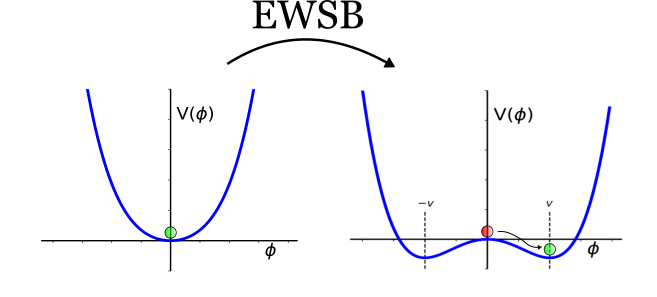
\includegraphics[width=0.75\textwidth]{figures/chapter1/higgs_potential_trans}
		\caption{Illustration of electroweak symmetry breaking (EWSB).
			\textbf{\textit{Left}}: Higgs potential with $\mu^2>0$ with stable equilibrium at $\phi=0$.
			\textbf{\textit{Right}}: With $\mu^2<0$, $\phi=0$ is no longer
			a stable equilibrium and the Higgs attains a non-zero vacuum
			expectation value at $\pm v$ --- breaking the \SUewk~gauge symmetry of the electroweak
			sector of the SM.
		}
	\label{fig:higgs_ewsb}
	\end{center}
\end{figure}

As opposed to `eating' gauge degrees of freedom as in the case of the \fieldWpm~and \fieldZ~bosons,
the fermion masses are obtained by adding additional interaction terms to \SML~between the
fermions and Higgs fields,
\begin{align}
	\mathcal{L}_{f-h} = y_f \left( \bar{L} \phi e^-_R + \phi^{\dagger} \overline{e^-}_R L\right).
	\label{eq:higgs_fermion_int}
\end{align}
Since both $L$ and $\phi$ are \SUtwo~doublets, adding the right-handed \SUtwo~singlet terms
do not spoil the \SUtwo~symmetry.
When the Higgs field acquires a non-zero vev after EWSB, we can insert Equation~\ref{eq:higgs_perturb} into Equation~\ref{eq:higgs_fermion_int} to obtain expressions for the fermions masses,
\begin{align}
	m_f = y_f \frac{v}{\sqrt{2}},
	\label{eq:fermion_mass_term}
\end{align}
where the $y_f$ are referred to as the fermion \textit{Yukawa couplings}, and are free parameters
of the SM that need to be measured.
Additional interactions arise between the fermions and $h(x)$ whose couplings are related
to the fermion masses as,
\begin{align}
	\mathcal{L}_{f-h} \propto \frac{m_f}{v} \bar{f}f h.
	\label{eq:higgs_fermion_coupling}
\end{align}

The general form Equation~\ref{eq:higgs_fermion_int} implies that the $y_f$ are matrices representing the
Higgs-fermion Yukawa couplings. They can be diagonalized by performing the proper unitary
transformations between the weak- and mass-bases of the fermion fields. In the case of the leptons,
this rotation is the identity: the lepton's weak eigenbasis is the same as their mass eigenbasis.
This is mainly due to the extraordinarily large mass difference between the charged and neutral
leptons within each lepton generation~\cite{Akhmedov:2007fk}. Within the quark-sector,  however,
the mass- and weak-basis fermion fields differ. This implies that the diagonalization procedure results
in mixing among the weak eigenstates of the quark fields to produce the observed mass eigenstates; i.e. the quark mass-eignstates ($d$,
$s$, $b$) are
coherent mixtures of the weak eigenstates ($d^{\prime}$,
$s^{\prime}$, $b^{\prime}$).\footnote{The mixing can be parametrised as either occurring between
the up-type, down-type, or a mixture of up- and down-type fields of each \SUtwo~doublet. Without
loss of generality and for simplicity, it is usually given with respect to the down-type quark fields as shown
here.}
This allows for the flavor-changing processes that are present
in charged weak interactions, allowing for interaction terms involving the decay
of a quark of one family into that of another family. The amount of mixing in the quark sector
is dictated by a $3\times 3$ unitary matrix known as the \textit{Cabibbo-Kobayashi-Maskawa} (CKM)
matrix~\cite{Kobayashi:1973fv} $\mathcal{V}_{\text{CKM}}$, the general form of which has four free parameters: three mixing angles
and a complex phase, $\delta$. The off-diagonal terms of the CKM matrix and the value of the mixing angles
dictate the amount of flavor mixing in the quark sector. The complex phase $\delta$
allows for charge-parity (CP) symmetry violating effects to occur. In fact, this term is the \textit{only} term of the SM
that allows for CP-violation --- an effect important for providing interactions that are asymmetric
between matter and anti-matter fields.\footnote{Charge Parity (CP) symmetry refers to the invariance
	of a theory with respect to swapping particles with their corresponding anti-particles and, additionally,
	inverting a field's spatial coordinates, $\psi(\vec{x}) \rightarrow \psi(-\vec{x})$. The former
	is the `C' symmetry and the latter is the `P' symmetry.
}

The remaining terms of $V(\phi)$ (Equation~\ref{eq:higgs_potential}) involve only the Higgs field. After
EWSB and the Higgs field acquiring vev we obtain,
\begin{align}
	V(\phi) \rightarrow V(\phi)_{\text{EWSB}} =  -\lambda \nu^2 h^2 - \lambda \nu h^3 - \frac{1}{4} \lambda h^4 + \text{const.}
	\label{eq:higgs_potential_self_int}
\end{align}
where we have ignored the terms already discussed above. The first term of Equation~\ref{eq:higgs_potential_self_int}
is the Higgs boson mass term, the second and third are the triple and quartic Higgs self-couplings,
\begin{align}
	\underbrace{m_{h} = \sqrt{ - 2 \mu^2} = \sqrt{ 2 \lambda v^2 }}_\text{Higgs boson mass} \hspace{1cm} \underbrace{\mathcal{L}_{hhh} \propto \frac{m_h^2}{v} \hspace{1cm} \mathcal{L}_{hhhh} \propto \frac{m_h^2}{v^2}}_\text{Triple and quartic Higgs self-couplings}.
	\label{eq:higgs_self_couplings}
\end{align}





%%%%%%%%%%%%%%%%%%%%%%%%%%%%%%%%%%%%%%%%%%%
%%%%%%%%%%%%%%%%%%%%%%%%%%%%%%%%%%%%%%%%%%%
%% sub section describing the standard model finally and its successes
%%%%%%%%%%%%%%%%%%%%%%%%%%%%%%%%%%%%%%%%%%%
%%%%%%%%%%%%%%%%%%%%%%%%%%%%%%%%%%%%%%%%%%%
\section{The Complete Standard Model, Successes and Shortcomings}
\label{sec:final_sm_description}

The physical field content of the SM, after EWSB, is detailed in Table~\ref{tab:sm_content_EWSB}
Also shown in Table~\ref{tab:sm_content_EWSB} are the electric charge associated with each
particle field, $Q$, the relevant couplings, and particle masses.


\begin{table}[!htb]
    \caption{
        The particle content of the SM after the process of
        electroweak symmetry breaking.
    }
    \begin{center}
        \begin{tabularx}{1\textwidth}{m{1em} c c c c }
        \toprule
        \hline
        & Physical Field & Q & Coupling & Mass [GeV] \\
        \hline
        \rotatebox{90}{\hspace{-0.1cm}\textbf{Quarks} } 
            & \makecell{ \quarkU, \quarkC, \quarkT \\ \quarkD, \quarkS, \quarkB} % FIELD
            & \makecell{ $2/3$ \\ $-1/3$ }% Q
            %& \makecell{ $\mathbf{3}$ \\ $\mathbf{3}$ } % SU(3)
            & \makecell{ ($y_i=$) $1\times10^{-5}$, $7\times10^{-3}$, $1$ \\ ($y_i=$) $3\times10^{-5}$, $5\times10^{-4}$, $0.02$ } % Coupling
            & \makecell{ $2\times10^{-3}$, $1.27$, $173$ \\ $4\times10^{-4}$, $0.10$, $4.18$ }\\% Mass
        \rotatebox{90}{\hspace{-0.1cm}\textbf{Leptons} } 
            & \makecell{ \leptonE, \leptonMu, \leptonTau \\ \neutrinoE, \neutrinoMu, \neutrinoTau } % FIELD
            & \makecell{ $-1$ \\ $0$ }% Q
            %& \makecell{ $\mathbf{1}$ \\ $\mathbf{1}$ } % SU(3)
            & \makecell{ ($y_i=$) $3\times10^{-7}$, $6\times10^{-4}$, $0.01$ \\ -- } % Coupling
            & \makecell{ $5\times10^{-4}$, $0.106$, $1.777$ \\ --}\\% Mass
        \midrule
        \rotatebox{90}{\textbf{Bosons} } 
            & \makecell{ \fieldPhoton \\ \fieldZ \\ (\fieldWp, \fieldWm) \\ \fieldG } % FIELD
            & \makecell{ $0$ \\ $0$ \\ $(+1,-1)$ \\ $0$ }% Q
            %& \makecell{ $\mathbf{1}$ \\ $\mathbf{1}$ \\ $\mathbf{1}$ \\ $\mathbf{8}$ } % SU(3)
            & \makecell{ $\alpha_{\text{EM}} \simeq 1/137$ \\ $\sin \theta_{W} \simeq 0.5$ \\ -- \\ $\alpha_s \simeq 0.1$ } % Coupling
            & \makecell{ $0$ \\ $91.2$ \\ $80.4$ \\  $0$}\\% Mass
        \midrule
        \rotatebox{90}{\textbf{Higgs} } 
            & \makecell{ \fieldH } % FIELD
            & \makecell{ $0$ }% Q
            %& \makecell{ $\mathbf{1}$ } % SU(3)
            & \makecell{ $\lambda$, $\mu$ } % Coupling
            & \makecell{ $125.09$ }\\% Mass

         %&   \makecell{ (\quarkUl, \quarkDl), (\quarkCl, \quarkSl), (\quarkTl, \quarkBl) \\ \quarkUr \\ \quarkDr}% CONTENT
         %&   \makecell{ $1/2$ \\ $1/2$ \\ $1/2$} % SPIN
         %&   \makecell{ $\mathbf{2}$ \\ $\mathbf{1}$ \\ $\mathbf{1}$}% SU(2)
         %&   \makecell{ $\mathbf{3}$ \\ $\mathbf{3}$ \\ $\mathbf{3}$}\\ % SU(3)
        %%\cdashline{1-7}
        %rotatebox{90}{\hspace{-0.1cm}\textbf{Leptons} }
         %&   \makecell{\quarkLi \\ \quarkEri} % FIELD
         %&   \makecell{ (\quarkEl, \quarkNuEl), (\quarkMul, \quarkNuMul), (\quarkTaul, \quarkNuTaul) \\ \quarkEr, \quarkMur, \quarkTaur}% CONTENT
         %&   \makecell{ $1/2$ \\ $1/2$ }% SPIN
         %&   \makecell{ $\mathbf{2}$ \\ $\mathbf{1}$ }% SU(2)
         %&   \makecell{ $\mathbf{1}$ \\ $\mathbf{1}$ } \\ % SU(3)
        %midrule
        %rotatebox{90}{\textbf{\stackanchor{Gauge}{Fields}} }
         %&   \makecell{\quarkB \\ \quarkW \\ \quarkG } % FIELD
         %&   \makecell{ \quarkB \\ (\quarkWone, \quarkWtwo, \quarkWthree) \\ \quarkG }% CONTENT
         %&   \makecell{ $1$ \\ $1$ \\ $1$} % SPIN
         %&   \makecell{ $\mathbf{1}$ \\ $\mathbf{3}$ \\ $\mathbf{1}$}% SU(2)
         %&   \makecell{ $\mathbf{1}$ \\ $\mathbf{1}$ \\ $\mathbf{8}$}\\ % SU(3)
        %midrule
        %rotatebox{90}{\textbf{\stackanchor{Higgs}{Field}}} 
         %&   \makecell{\quarkPhi } % FIELD
         %&   \makecell{ (\quarkPhip, \quarkPhizero) }% CONTENT
         %&   \makecell{ $0$  } % SPIN
         %&   \makecell{ $\mathbf{2}$ }% SU(2)
         %&   \makecell{ $\mathbf{1}$ }\\ % SU(3)
        \hline
        \bottomrule
        \end{tabularx}
    \end{center}
    \label{tab:sm_content}
\end{table}


%%%%%%%%%%%%%%%%%%%%%%%%%%%%%%%%%%%%%%%%%%%%%%%%%%%%%%%%%%%%%%%%%%%%%%%%%%%%%%%%%
%%%%%%%%%%%%%%%%%%%%%%%%%%%%%%%%%%%%%%%%%%%%%%%%%%%%%%%%%%%%%%%%%%%%%%%%%%%%%%%%%
%%%%%%%%%%%%%%%%%%%%%%%%%%%%%%%%%%%%%%%%%%%%%%%%%%%%%%%%%%%%%%%%%%%%%%%%%%%%%%%%%
%
% SUCCESSES
%
%%%%%%%%%%%%%%%%%%%%%%%%%%%%%%%%%%%%%%%%%%%%%%%%%%%%%%%%%%%%%%%%%%%%%%%%%%%%%%%%%
%%%%%%%%%%%%%%%%%%%%%%%%%%%%%%%%%%%%%%%%%%%%%%%%%%%%%%%%%%%%%%%%%%%%%%%%%%%%%%%%%
%%%%%%%%%%%%%%%%%%%%%%%%%%%%%%%%%%%%%%%%%%%%%%%%%%%%%%%%%%%%%%%%%%%%%%%%%%%%%%%%%

\subsection{Successes of the Standard Model}
\label{sec:sm_successes}

The particle content presented in Table~\ref{tab:sm_content_EWSB} represents the current
picture of the visible matter content of the Universe.
It is a concise picture.
With this particle content in hand, and the description of their fundamental particle interactions (Equation~\ref{eq:sm_lagrangian}, after EWSB),
the predictive power of the SM is immense.

Figure~\ref{fig:sm_xsec_summary} shows a summary of LHC measurements of cross-sections
for various production processes at 7, 8, and 13\,TeV.
The agreement of these measurements with the theoretical predictions provided by the SM, spanning over 10 orders of magnitude,
is an incredible testament to the power of the SM and the toolkit provided by QFT.
The power of the SM, and its internal consistency, is illustrated in Figure~\ref{fig:mw_mt_scan},
which shows the results of indirect measurements of the $W$-boson and top-quark masses based
on fits to electroweak precision data.
When all measurements other than those on $m_h$ are included, the constraints of the SM
only allow for a small region of the $(m_{\text{top}}, M_W)$ parameter space.
Adding the Higgs mass measurement results only shrinks this allowed area.
The fact that these indirect measurements agree so well with the direct measurements paints a picture
of the SM as being a fundamentally complete picture of the known physical phenomena.
It is likely that if the SM were not accounting for particular types of interactions or fields,
the level of agreement between the direct measurements and those obtained indirectly via
fits to electroweak precision data would not be to the level seen in Figure~\ref{fig:mw_mt_scan}.

\begin{figure}[!htb]
    \begin{center}
        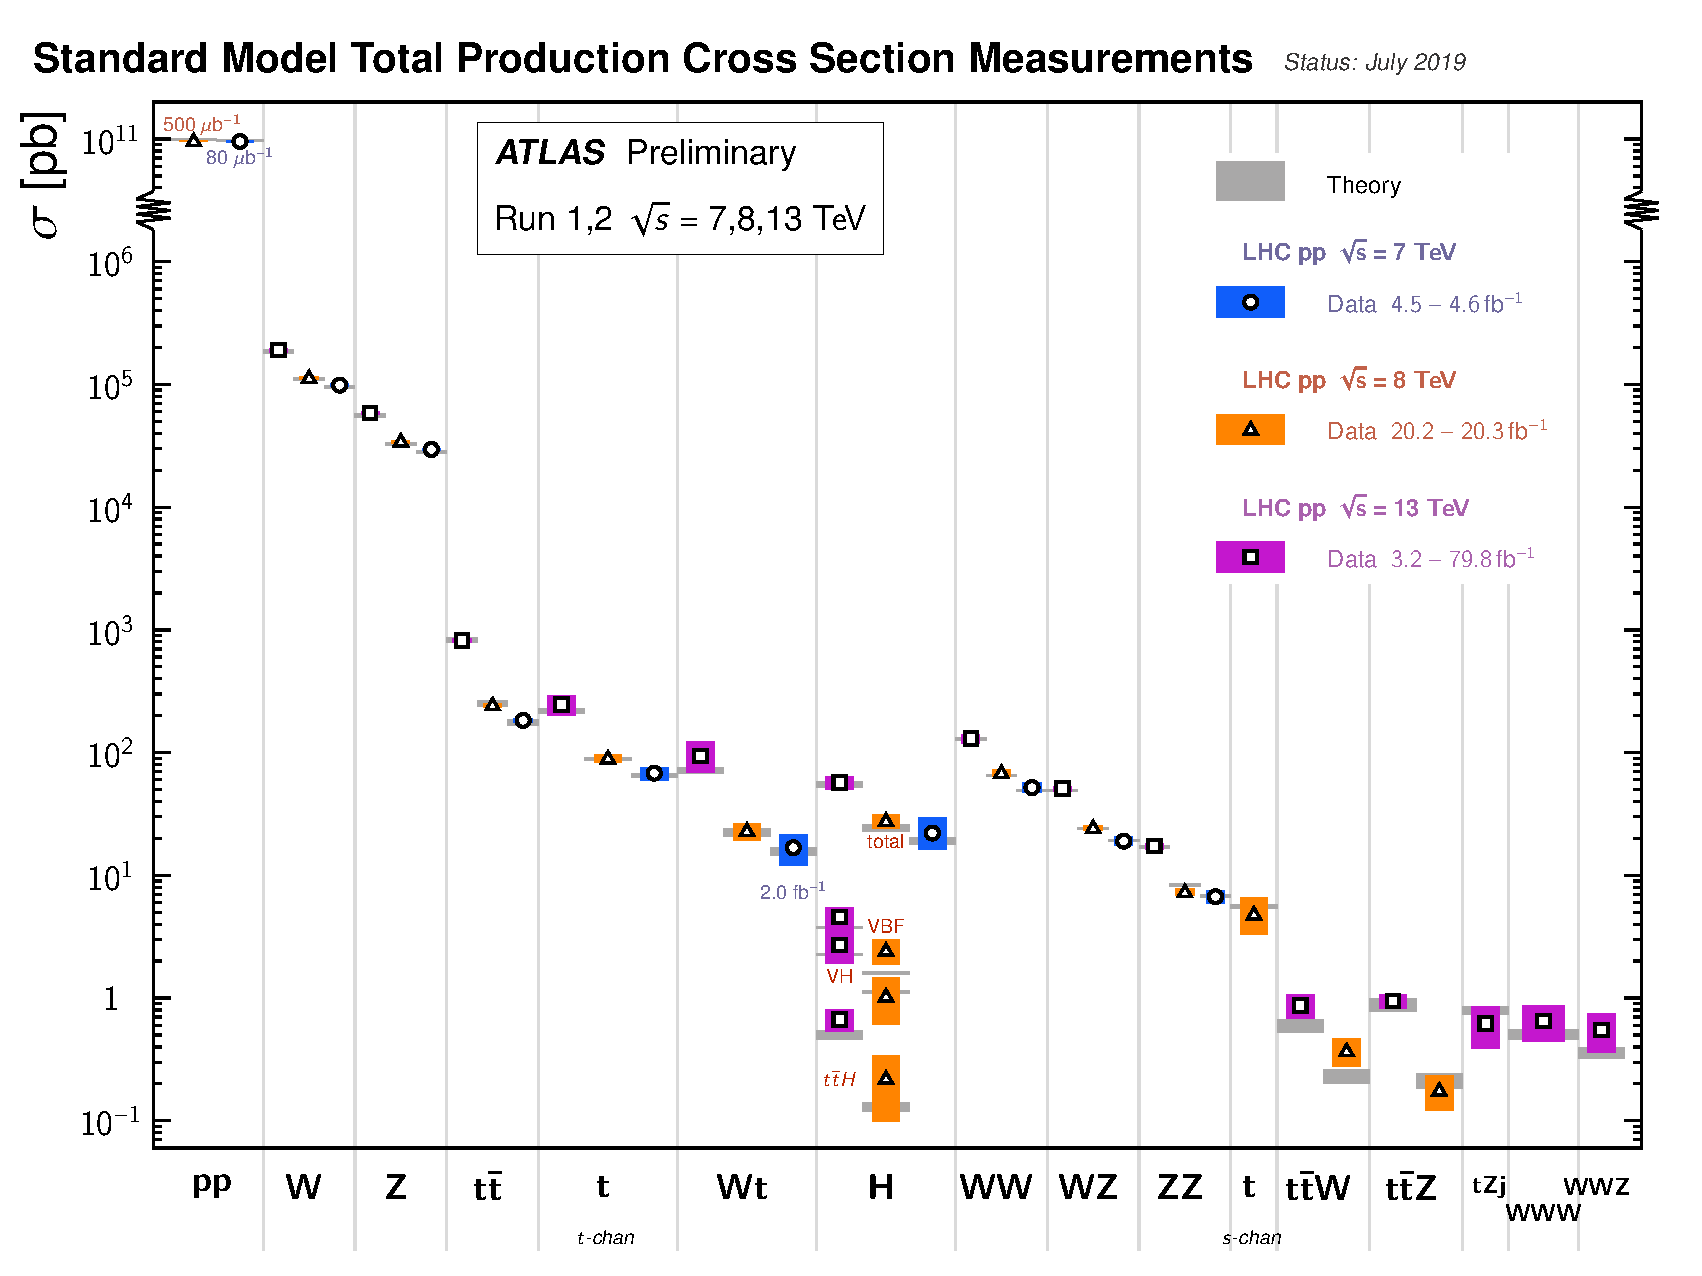
\includegraphics[width=0.75\textwidth]{figures/chapter1/sm_final/sm_xsec_summary}
        \caption{
            Summary of several Standard Model total production cross section measurements,
            corrected for branching fractions, compared to the corresponding theoretical expectations. 
        }
        \label{fig:sm_xsec_summary}
    \end{center}
\end{figure}
\begin{figure}[!htb]
    \begin{center}
        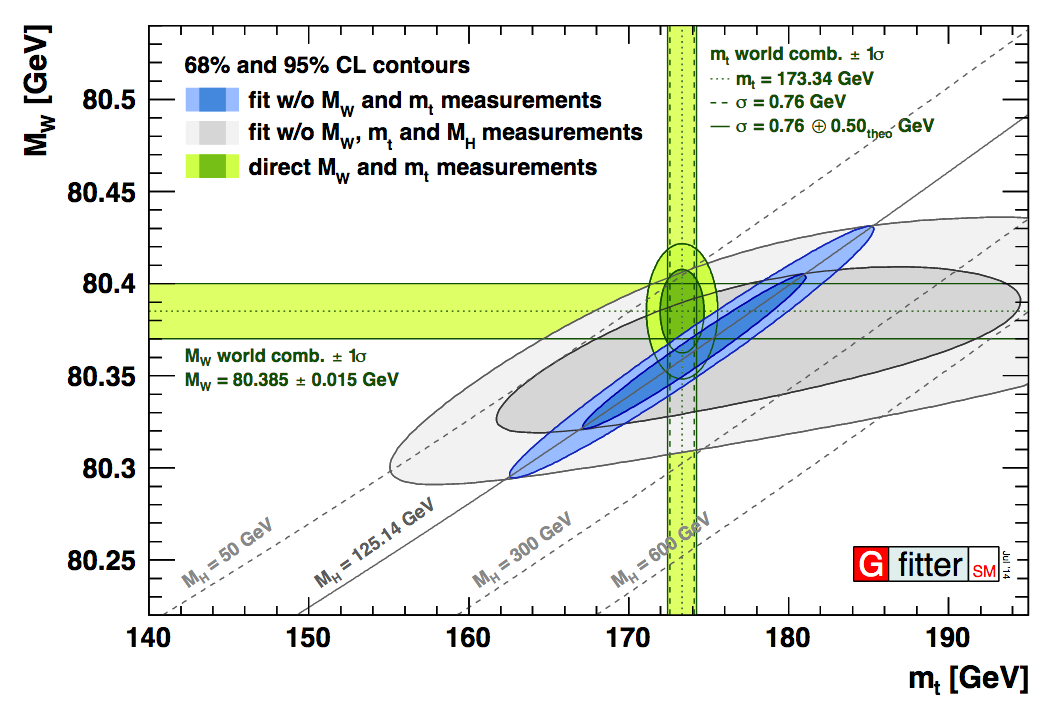
\includegraphics[width=0.65\textwidth]{figures/chapter1/sm_final/mw_vs_mt_indirect}
        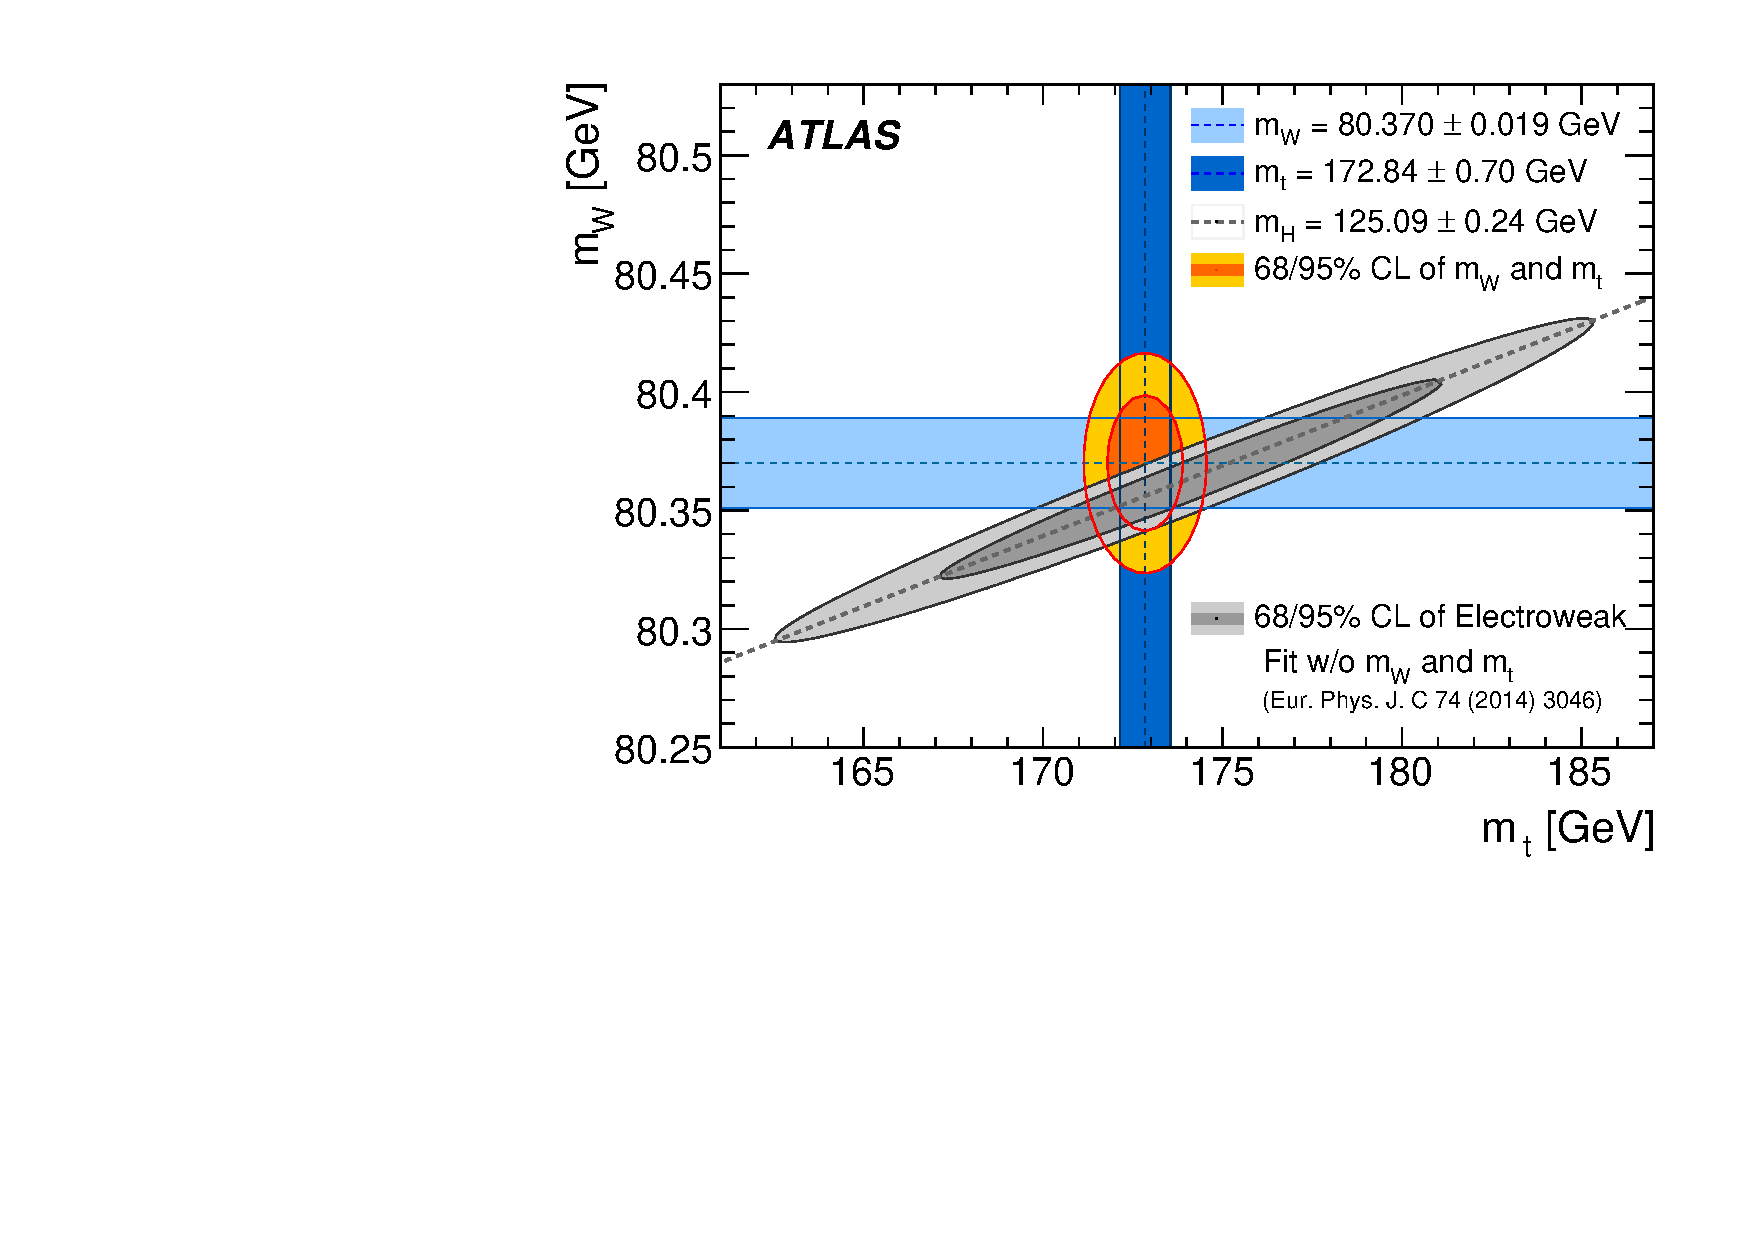
\includegraphics[width=0.69\textwidth]{figures/chapter1/sm_final/atlas_w_boson_mass_mw_mt}
        \caption{
            Contours at 68\% and 95\% CL obtained from scans of $M_W$ versus $m_{\text{top}}$,
            for the global electroweak fits in comparison to the direct measurements.
            \textit{\textbf{Top}}: Including Higgs boson mass measurements in the indirect fit~\cite{HMassATLAS,HMassCMS} (blue)
                or excluding them (grey). From Ref.~\cite{GFitter}.
            \textit{\textbf{Bottom}}: Including the latest precision $W$-boson mass measurement from the ATLAS
                experiment. From Ref.~\cite{ATLASWMass}.
%            for the global electroweak fit including the Higgs boson mass ($m_h$) measurements~\cite{HMassATLAS,HMassCMS} (blue)
%            and excluding the $m_h$ measurements (grey), as compared t the direct
%            measurements of these quantities (green bands and ellipses).
%            From Ref.~\cite{GFitter}.
        }
        \label{fig:mw_mt_scan}
    \end{center}
\end{figure}

With the discovery a Higgs boson like particle with a mass at 125\,GeV in 2012~\cite{HDiscoveryATLAS,HDiscoveryCMS},
the final piece of the SM described by Equation~\ref{eq:sm_lagrangian} is potentially found.
The 2012 Higgs discovery meant the start of a very long experimental program, focused
on studying this new particle and confirming its role as being the fundamental scalar boson, $\phi$,
appearing in the SM.

It should be stressed that the terms associated with the Higgs potential appearing in the SM
Lagrangian, given by Equation~\ref{eq:higgs_potential}, are by no means fundamental.
They do not have to appear in this way.
The terms appearing in Equation~\ref{eq:higgs_potential} take the form they do since they
could lead to masses for the fermions and gauge bosons.
There is no fundamental symmetry motivating their precise form.
The BEH mechanism is inspired by that of super-conductivity, in which the formation composite (i.e. not elementary)
scalar particles --- the Cooper pairs --- occurs.
%The BEH mechanism is inspired by the formation of composite (i.e. not elementary) scalar particles
%appearing in super-conductivity (Cooper pairs).
The fact that the same type of phase transition should describe the generation of masses for
the elementary particles of the SM, and that it should presuppose the existence of an \textit{elementary}
scalar boson, was simply left as one of the last open questions of the SM.
In a sense, the truth of the form underlying Equation~\ref{eq:higgs_potential} was not important to BEH.
The more important takeaway was that there \textit{could} be a mechanism by which the SM particles acquired
mass without disrupting the fundamental gauge structure of the SM that had already held up to experimental scrutiny.
%In a certain sense, this is reflected by the fact that BEH were awarded the Nobel prize only \textit{after} the discoveries of the ATLAS and CMS experiments
%in 2012, whereas GWS were awarded theirs several years \textit{before} the experimental verification of
%the existence of the $W$ and $Z$ bosons.

It is then up to the experiments to verify that the 125\,GeV scalar boson discovered in 2012
is responsible for the BEH mechanism as described in Section~\ref{sec:higgs_description}.
The form of the Higgs potential as defined in Equation~\ref{eq:higgs_potential} makes
very clear predictions on the form and strengths of the couplings to the known fundamental particles:
the gauge bosons and fermions, with couplings to the Higgs predicted to take the forms
of Equations~\ref{eq:higgs_gauge_couplings} and \ref{eq:higgs_fermion_coupling}, respectively.
It is then up to the ATLAS and CMS experiments to verify that the new particle couples
to these `old' particles just as predicted.
The coupling strengths also dictate the Higgs decay rates into specific SM particles, as indicated
in Figure~\ref{fig:higgs_br_sm}.
Any deviation with respect to the SM-predicted values in the measurement of the Higgs decay branching ratios, or
in the values of the fermion or gauge coupling strengths and their dependence on the
particle masses, would indicate that the particle discovered in 2012 is not the Higgs boson as predicted
in the SM.

All of the measurements of the properties of the 125 GeV particle
made by the ATLAS and CMS experiments are so far in fairly good agreement with the SM prediction
of a $m_h = 125$ GeV Higgs boson~\cite{HProp0,HProp1,HProp2,HProp3,HProp4,HProp5,HProp6,HProp7,HProp8}.
The agreement with the SM prediction, over a wide variety of measurements, is illustrated in
Figure~\ref{fig:higgs_measurements} which shows the measurements of the fermion and gauge
couplings and of the cross-sections of the leading Higgs production mechanisms and decay
branching ratios.
Within the precision of these measurements, the SM is fully supported by the experiments
and it appears as though the particle discovered in 2012 is in fact the particle as predicted
by BEH.

\begin{figure}[!htb]
    \begin{center}
        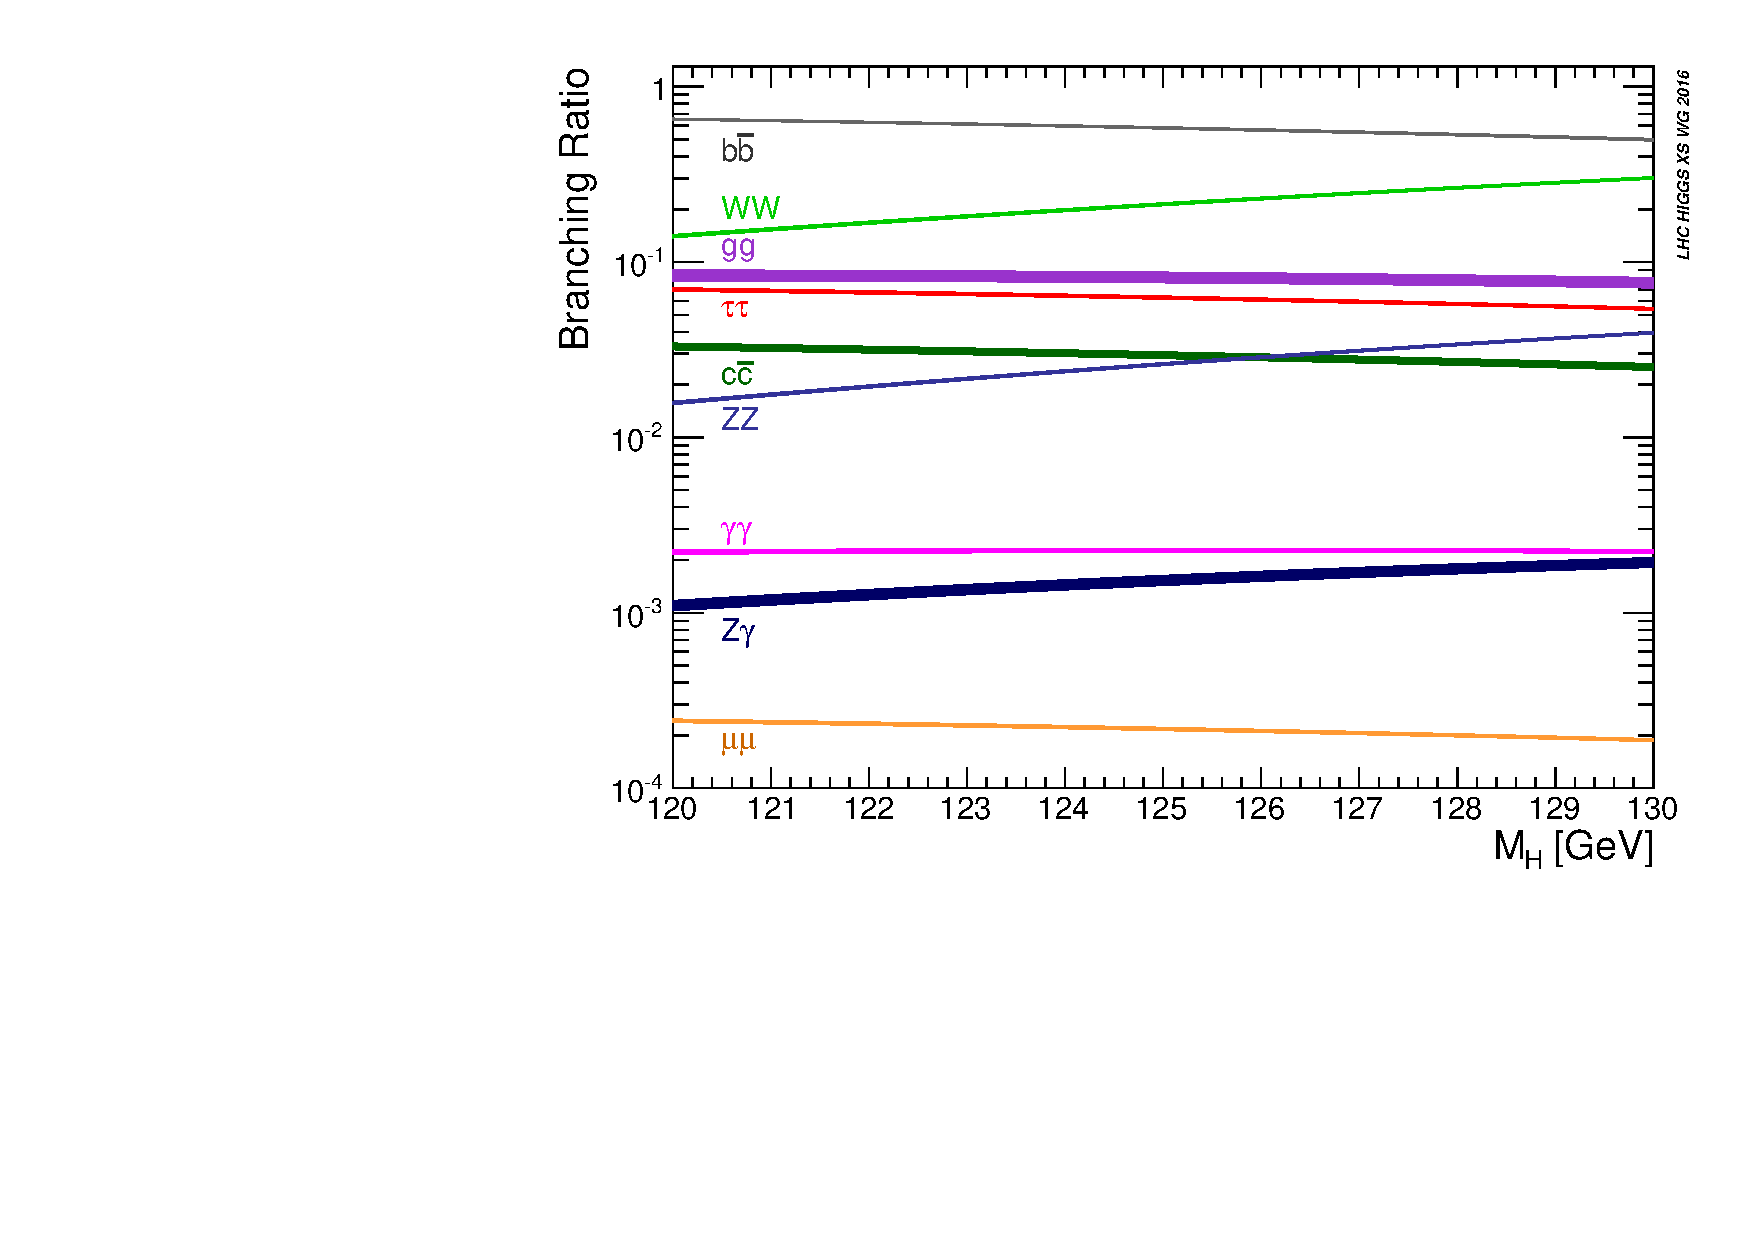
\includegraphics[width=0.6\textwidth]{figures/chapter1/sm_final/higgs_br_sm}
        \caption{
            Predicted branching ratios for an SM-like Higgs boson with $m_{h} = 125\,\GeV$.
        }
        \label{fig:higgs_br_sm}
    \end{center}
\end{figure}

\begin{figure}[!htb]
    \begin{center}
        \raisebox{1cm}{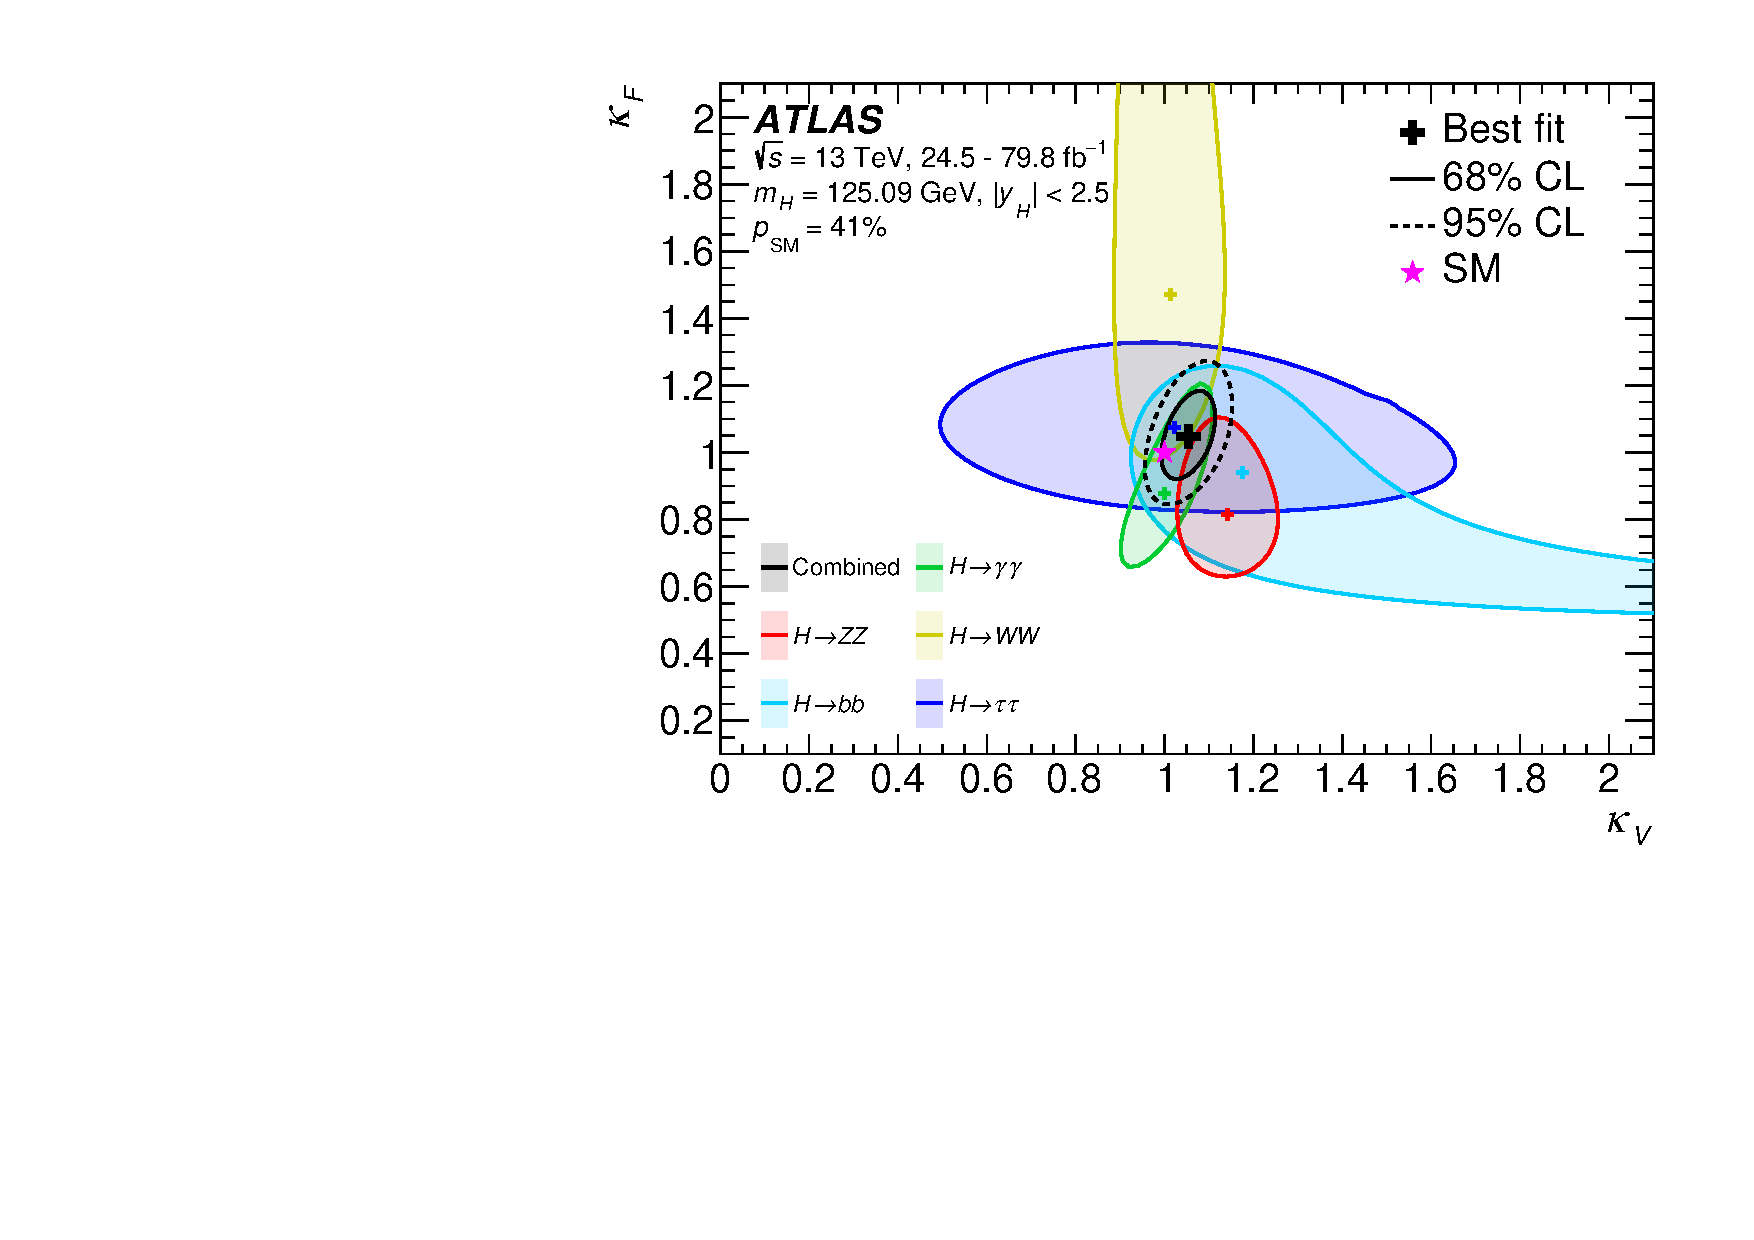
\includegraphics[width=0.49\textwidth]{figures/chapter1/sm_final/higgs_kappa_v_f}}
        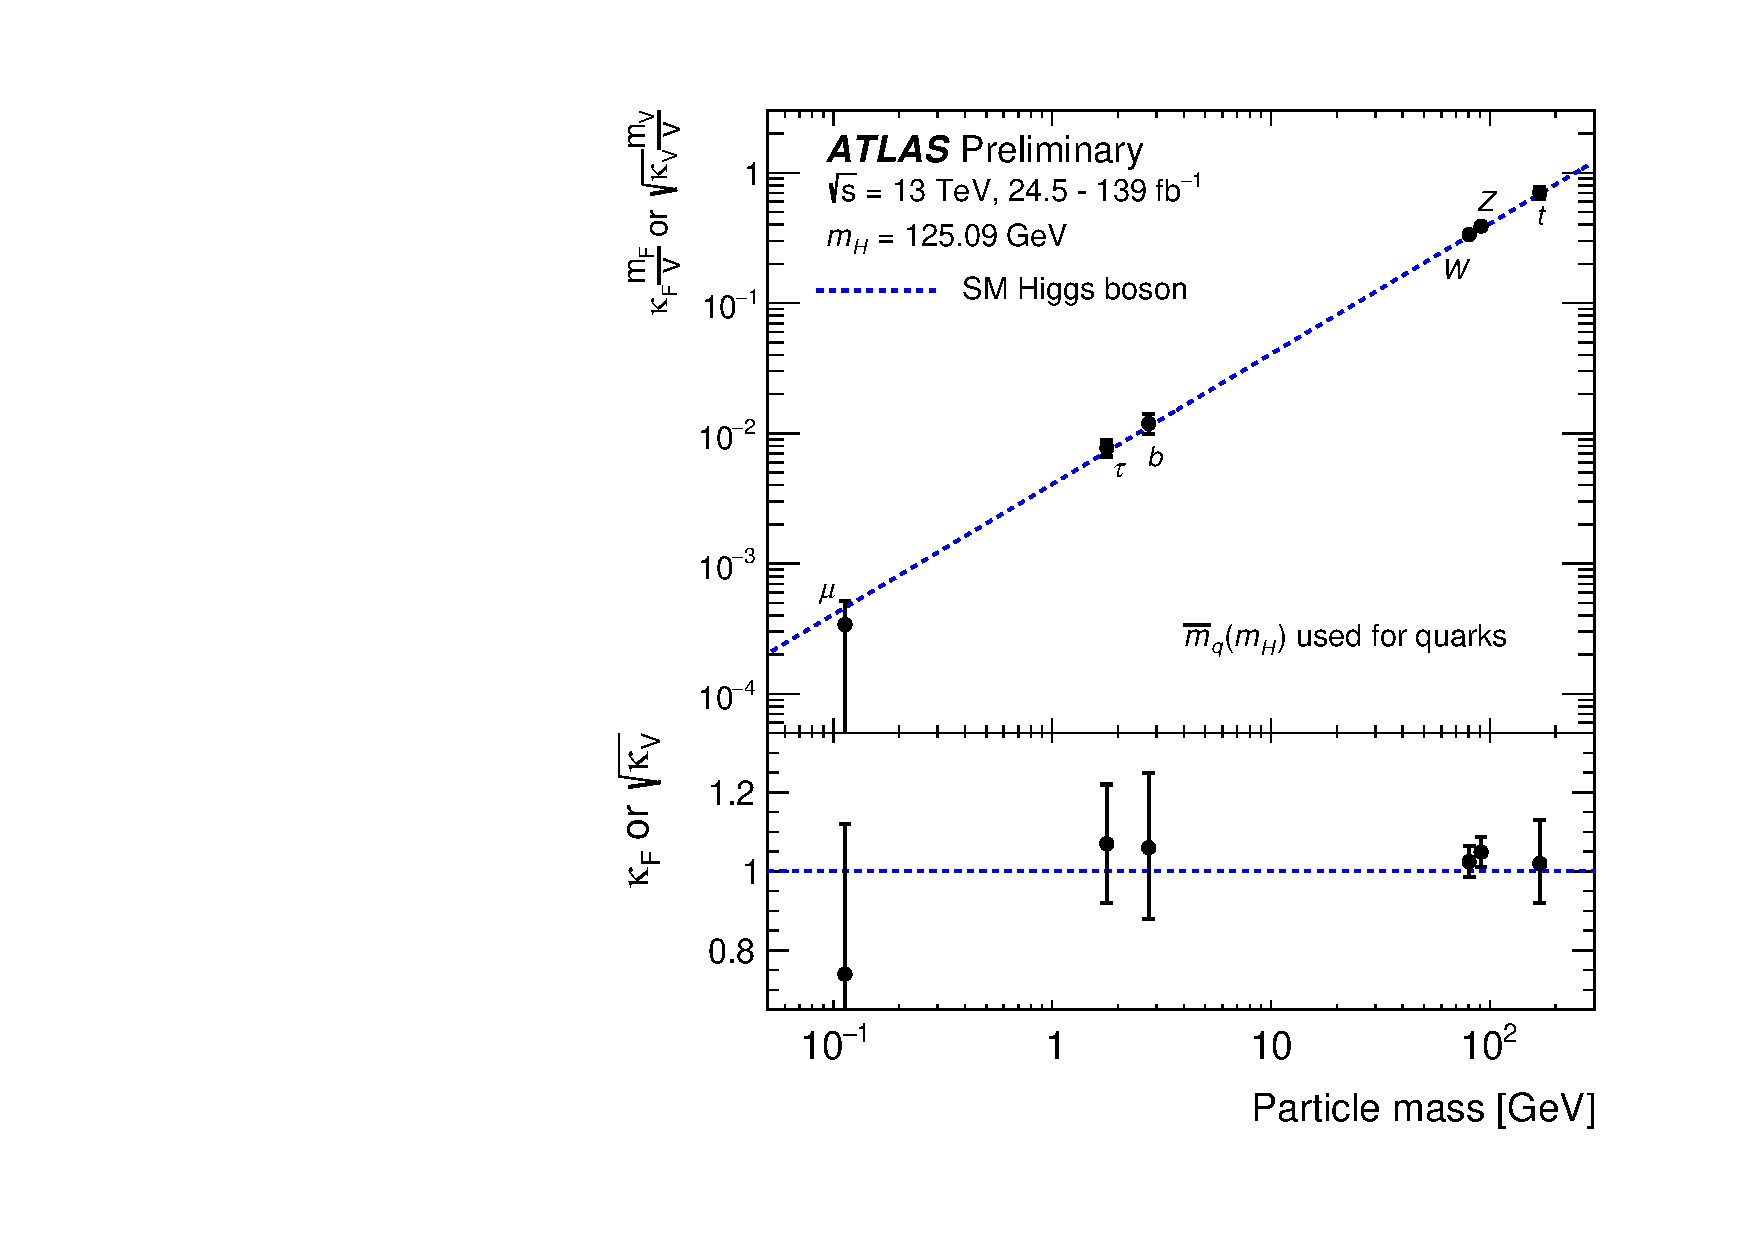
\includegraphics[width=0.49\textwidth]{figures/chapter1/sm_final/higgs_kappa_vs_mass}
        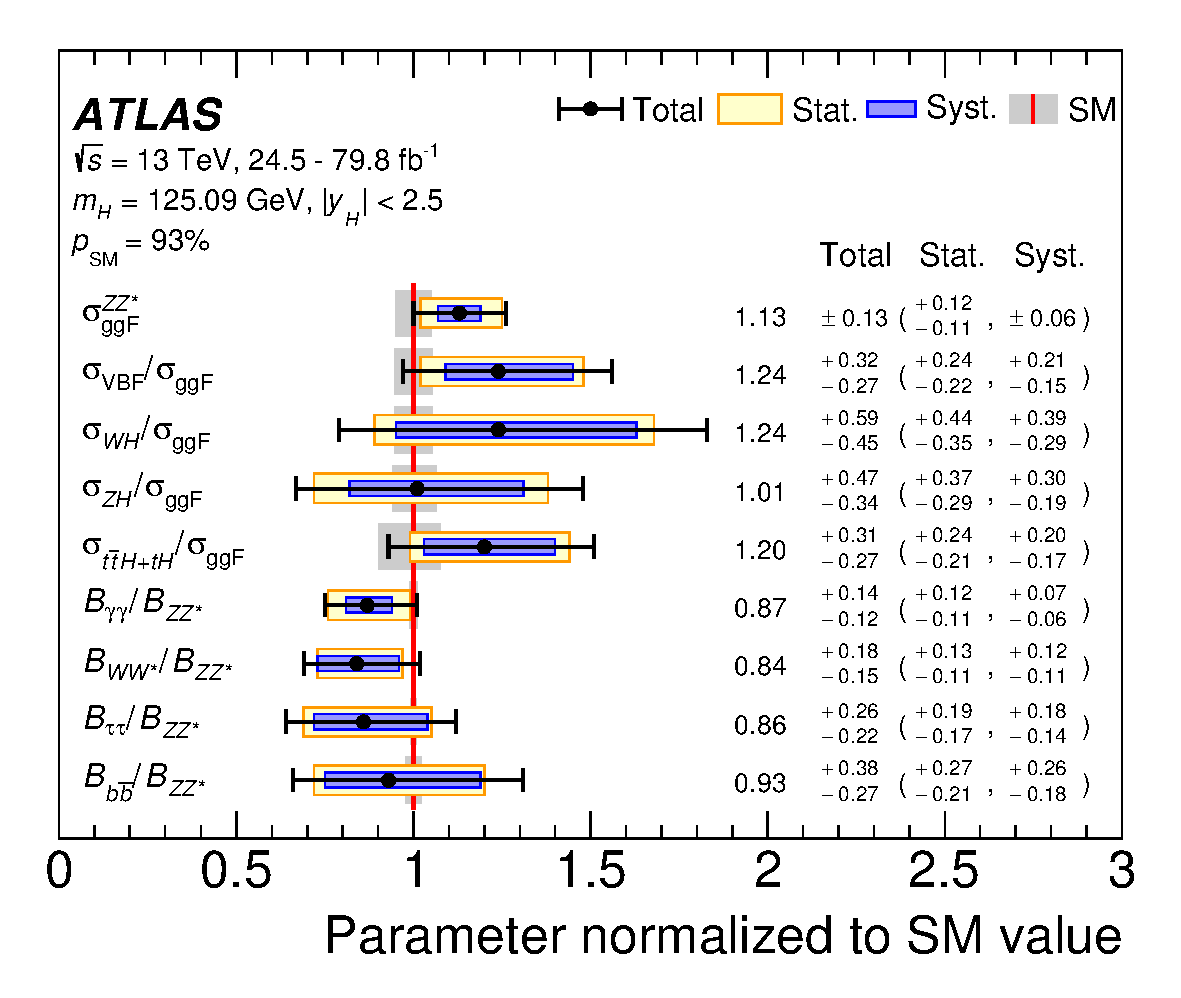
\includegraphics[width=0.49\textwidth]{figures/chapter1/sm_final/higgs_prod_and_br}
        \caption{
            Higgs precision measurements of couplings to SM particles.
            Figures from Ref.~\cite{HiggsProps}.
            \textit{\textbf{Left}}: Combined measurement of fermion and gauge-boson Higgs coupling modifiers, $\kappa_f$
                and $\kappa_V$ (assumed to be universal across fermion and gauge-boson species in the result pictured).
                Values of $\kappa_f$ or $\kappa_V$ equal to 1 correspond to the SM prediction for the Higgs' couplings to
                these particles.
            \textit{\textbf{Right}}: Measured values of the Higgs fermion and gauge-boson coupling parameters
                as a function of the fermion and gauge-boson masses.
                The blue dashed line shows the SM prediction (Equations~\ref{eq:higgs_gauge_couplings} and \ref{eq:higgs_fermion_coupling}).
            \textit{\textbf{Bottom}}: Measurements of Higgs production cross sections and (relative) decay branching ratios.
        }
        \label{fig:higgs_measurements}
    \end{center}
\end{figure}

In addition to the Higgs couplings to the SM fermions and gauge bosons, the SM Lagrangian
predicts terms describing the Higgs \textit{self}-couplings.
These terms are described by the $\lambda$ parameter in Equation~\ref{eq:higgs_potential}
and appearing in Table~\ref{tab:sm_content_EWSB}.
The Higgs self-coupling parameter $\lambda$ has a value predicted by the SM, as seen in 
Equation~\ref{eq:higgs_self_couplings}, which is fixed by the Higgs boson mass.
The parameter $\lambda$ is directly responsible for providing the structure of the Higgs potential,
indicated by Equation~\ref{eq:higgs_potential_self_int}, and therefore plays a fundamental
role in EWSB.
Measuring how the 125\,GeV Higgs boson couples and decays to the SM fermions and gauge bosons,
then, is only a necessary requirement for confirming that the particle is the one predicted by
the SM: it is not sufficient.
To truly confirm that the 125\,GeV boson is indeed that predicted by the SM, and that EWSB
is described by the BEH mechanism, the Higgs self-coupling parameter will have to be measured
experimentally and confirmed to take its predicted value given by Equation~\ref{eq:higgs_self_couplings}.

Direct measurement of $\lambda$ proceeds only through the observation of events in which Higgs bosons
are produced in pairs.
At the LHC, this process occurs predominantly via gluon-gluon fusion through the two diagrams illustrated
in Figure~\ref{fig:hh_feynman}.
The triangle and box diagrams shown in Figure~\ref{fig:hh_feynman} represent destructively interfering amplitudes.
As a result, the cross-sections associated with the production of Higgs boson pairs is exceedingly low
and statistically significant observation of this process is not expected to occur until
near the end of the lifetime of the LHC.
The study of Higgs boson pairs is the subject of the analysis to be presented in Chapter~\ref{chap:search_hh}.

\begin{figure}[!htb]
    \begin{center}
        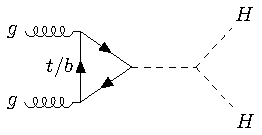
\includegraphics[width=0.7\textwidth]{figures/search_hh/feynman_diagrams/fdiagram_triangle}
        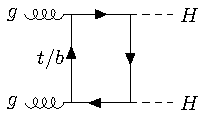
\includegraphics[width=0.55\textwidth]{figures/search_hh/feynman_diagrams/fdiagram_box}
        \caption{
            Representative Feynman diagrams that contribute at leading order in QCD to the non-resonant
            production of Higgs boson pairs.
            {\textbf{\textit{Top}}}: The `triangle' diagram, sensitive to the Higgs self-coupling, $\lambda$.
            {\textbf{\textit{Bottom}}}: The `box' diagram, sensitive to the (squared) Yukawa couplings to the third generation
            fermions entering the loop.
        }
        \label{fig:hh_feynman}
    \end{center}
\end{figure}

%%%%%%%%%%%%%%%%%%%%%%%%%%%%%%%%%%%%%%%%%%%%%%%%%%%%%%%%%%%%%%%%%%%%%%%%%%%%%%%%%
%%%%%%%%%%%%%%%%%%%%%%%%%%%%%%%%%%%%%%%%%%%%%%%%%%%%%%%%%%%%%%%%%%%%%%%%%%%%%%%%%
%%%%%%%%%%%%%%%%%%%%%%%%%%%%%%%%%%%%%%%%%%%%%%%%%%%%%%%%%%%%%%%%%%%%%%%%%%%%%%%%%
%
% SHORTCOMINGS
%
%%%%%%%%%%%%%%%%%%%%%%%%%%%%%%%%%%%%%%%%%%%%%%%%%%%%%%%%%%%%%%%%%%%%%%%%%%%%%%%%%
%%%%%%%%%%%%%%%%%%%%%%%%%%%%%%%%%%%%%%%%%%%%%%%%%%%%%%%%%%%%%%%%%%%%%%%%%%%%%%%%%
%%%%%%%%%%%%%%%%%%%%%%%%%%%%%%%%%%%%%%%%%%%%%%%%%%%%%%%%%%%%%%%%%%%%%%%%%%%%%%%%%
\FloatBarrier
\subsection{Perceived Shortcomings of the Standard Model and Open Questions}
\label{sec:sm_shortcomings}

Despite the impressive results and predictive power of the SM illustrated in the previous
section, the SM is unable to provide a complete picture of what we now consider the observed
Universe.
A few items that are clearly not explained within the framework of the SM are described below.
%A few items that are clearly not explainable under the framework of the SM are described below.
Chapter~\ref{chap:bsm} goes on to introduce an extension to the SM that provides explanations
for many of these short comings of the SM.

\begin{description}
    \item[] \textbf{Existence of Dark Matter (DM) and Dark Energy (DE)} \\
        Most of the experimental evidence that we currently have that supports the notion that
        physics beyond the SM (BSM) exists comes not from collider-based particle physics experiments,
        but from astrophysical observations.
        Astrophysical observations suggest that the majority of the matter content of the Universe
        is composed of a non-luminous, weakly interacting type of matter referred to as `Dark Matter' (DM)
        and that the expansion of the Universe is accelerating, perhaps due to presence of
        `Dark Energy' (DE)~\cite{Davis:2014csa,PlanckCollab}.
        There has not yet been experimental proof of the particle nature of DM, but
        many theories suggest that it fall under the class of `Weakly Interacting Massive Particle' (WIMPs), i.e. that it be `WIMP-like'.
        The particle nature of DE is completely unknown and without a fundamental description.
    \item[] \textbf{Massive Neutrinos} \\ The observation of neutrino oscillations~\cite{Fukuda:1998mi} provides evidence
        in support of neutrinos having nonzero masses. This directly contradicts the massless neutrino hypothesis of the SM.
    \item[] \textbf{Matter-Antimatter Asymmetry} \\
        The only parameter in the SM that allows for CP violation is the CP-violating phase in the CKM matrix,
        which is unable to account for the amount of CP violation needed to account for the
        observed asymmetry in the amount of matter over antimatter in the Universe.
        Additional CP violating effects are necessary to account for this observed asymmetry and should be relevant
        to early-Universe cosmology~\cite{Sakharov_1991}.
    \item[] \textbf{The Hierarchy Problem} \\
        The Hierarchy Problem refers to the fact that the electroweak sector, through the scalar Higgs boson,
        is sensitive to high energy cut-off scales nearing the Planck Mass, $M_{P} \approx 10^{18}--10^{19}$\,GeV.
        This is evident when computing the higher-order corrections to the Higgs mass,
        \begin{align*}
            m_h^2 = m_{h,\,0}^2 + \Delta m_h^2,
        \end{align*}
        which are found to be quadratically divergent due to the fact that the Higgs is not protected by any fundamental
        internal symmetries:
        %\vspace{-1.2cm}
        \begin{align}
            \Delta m_h^2 = -\frac{ |y_f|^2 }{16 \pi^2} \left[ 2 \Lambda^2  + \mathcal{O} \left( m_f^2 \ln \left( \frac{\Lambda}{m_f} \right) \right) \right],
            \label{eq:higgs_divergence}
        \end{align}
        where $y_f$ is the fermion Yukawa coupling, $m_f$ is the associated fermion mass, and $\Lambda$ is the
        ultra-violate cut-off scale.
        Similar terms also appear for the SM gauge bosons, resulting in their own contributions like Equation~\ref{eq:higgs_divergence}, but given the near-unity Yukawa coupling of the top-quark,
        the divergence is most evident from the top-quark loop contributions to $\Delta m_h^2$, such as that shown in Figure~\ref{fig:higgs_mass_correction}.
        %the divergence is most sensitive to the fermion terms appearing in the above via $y_t$.
        \begin{figure}[!htb]
        \hspace{1.8cm}
        \begin{minipage}{0.8\textwidth}
            \begin{center}
                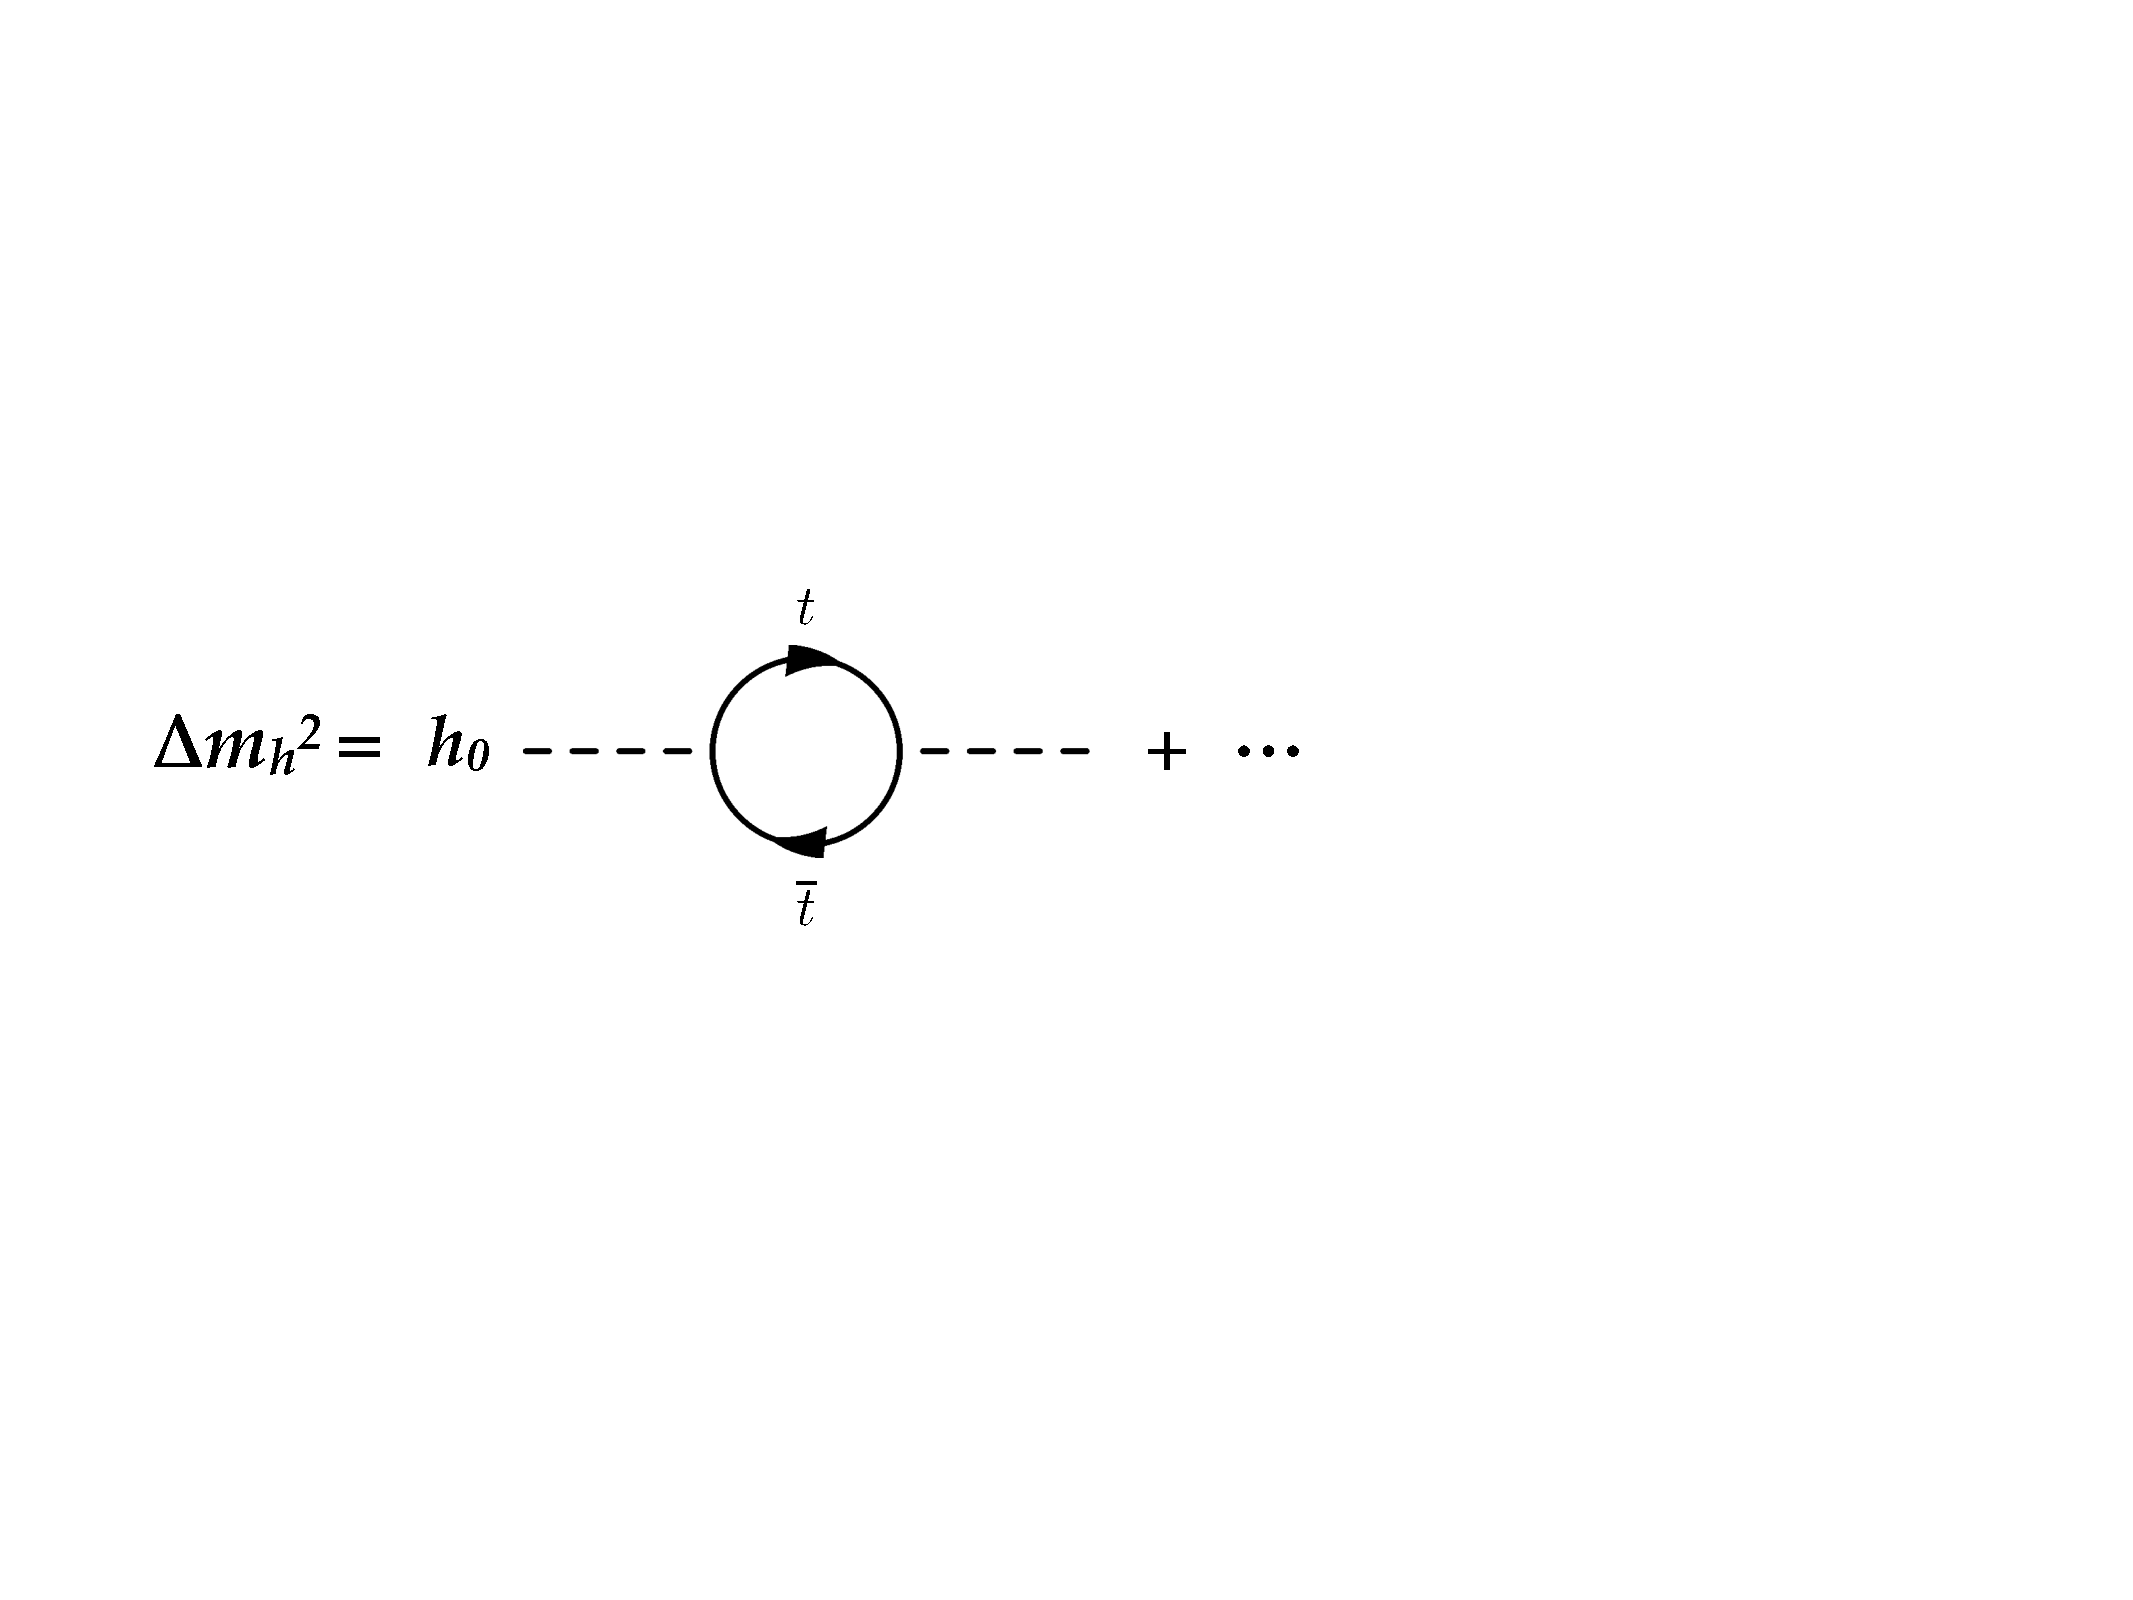
\includegraphics[width=0.6\textwidth]{figures/higgs_corr/higgs_mass_correctionsPDF}
                \caption{
                    Top-quark loop contribution to the higher-order computation of the Higgs mass that
                    leads to unregulated divergent terms such as Equation~\ref{eq:higgs_divergence}.
                }
                \label{fig:higgs_mass_correction}
            \end{center}
        \end{minipage}
        \end{figure}
        The apparent contradiction that the electroweak scale at which the Higgs boson is experimentally known to exist
        should also be unavoidably sensitive to $M_P$, attempting to drive the Higgs boson mass to values 16 orders
        of magnitude larger than the measured one,
        is at the heart of the Hierarchy Problem.
        The high energy scales at which SM calculations fail are typically assumed to be the scales
        at which new physics arise and take over as a more complete description of natural pheneomena.
        That the Higgs boson is apparently driven to these scales motivates the arguments in favor
        of their being new physics at or near the electroweak scale which act to cancel the quadratically
        divergent terms appearing in the Higgs mass corrections.
        That cancellations of terms on the order of $10^{30}$ ($\Lambda^2$) should be possible introduces the
        philosophical concerns of \textit{naturalness}, which ponder whether or not Nature is such
        that the additional sources of high energy physics --- not accounted for by the SM --- can conspire in such a way as to
        allow for such perfectly fine-tuned cancellation.
\end{description}

%eq:higgs_potential



%\section{Particles and Forces}
%
%Here we introduce the SM particle content and provide a description of the interactions that
%link the particles together.
%
%
\begin{table}[!htb]
    \caption{
        The particle content of the SM and their transformation
        properties under the SM gauge groups, prior to electroweak symmetry breaking.
        The representations of each of the gauge groups are shown in the three-right
        columns. The \Uone symmetry of weak-hypercharge transformations is one-dimensional
        and the column gives the weak-hypercharge $\mathcal{Y}$ associated with each
        field. For \SUthree and \SUtwo, $\mathbf{1}$ refers to the field belonging to
        the associated singlet representation, $\mathbf{2}$ to the doublet representation,
        $\mathbf{3}$ to the triplet representation, and $\mathbf{8}$ to the octet representation.
    }
    \begin{center}
        \begin{tabularx}{0.96\textwidth}{m{1em} c c c c c c }
        \toprule
        \hline
        & Field Label & Content & Spin & \Uone~($\mathcal{=Y}$) & \SUtwo & \SUthree \\
        \hline
        \rotatebox{90}{\hspace{-0.1cm}\textbf{Quarks} } 
         &   \makecell{\fieldQi \\ \fieldUri \\ \fieldDri} % FIELD
         &   \makecell{ (\fieldUl, \fieldDl), (\fieldCl, \fieldSl), (\fieldTl, \fieldBl) \\ \fieldUr \\ \fieldDr}% CONTENT
         &   \makecell{ $1/2$ \\ $1/2$ \\ $1/2$} % SPIN
         &   \makecell{ $1/6$ \\ $2/3$ \\ $-1/3$}% U(1)
         &   \makecell{ $\mathbf{2}$ \\ $\mathbf{1}$ \\ $\mathbf{1}$}% SU(2)
         &   \makecell{ $\mathbf{3}$ \\ $\mathbf{3}$ \\ $\mathbf{3}$}\\ % SU(3)
        %\cdashline{1-7}
        \rotatebox{90}{\hspace{-0.1cm}\textbf{Leptons} }
         &   \makecell{\fieldLi \\ \fieldEri} % FIELD
         &   \makecell{ (\fieldEl, \fieldNuEl), (\fieldMul, \fieldNuMul), (\fieldTaul, \fieldNuTaul) \\ \fieldEr, \fieldMur, \fieldTaur}% CONTENT
         &   \makecell{ $1/2$ \\ $1/2$ }% SPIN
         &   \makecell{ $1/2$ \\ $-1$ }% U(1)
         &   \makecell{ $\mathbf{2}$ \\ $\mathbf{1}$ }% SU(2)
         &   \makecell{ $\mathbf{1}$ \\ $\mathbf{1}$ } \\ % SU(3)
        \midrule
        \rotatebox{90}{\textbf{\stackanchor{Gauge}{Fields}} }
         &   \makecell{\fieldB \\ \fieldW \\ \fieldG } % FIELD
         &   \makecell{ \fieldB \\ (\fieldWone, \fieldWtwo, \fieldWthree) \\ \fieldG$_a$, $a\in[1,..,8]$ }% CONTENT
         &   \makecell{ $1$ \\ $1$ \\ $1$} % SPIN
         &   \makecell{ $0$ \\ $0$ \\ $0$}% U(1)
         &   \makecell{ $\mathbf{1}$ \\ $\mathbf{3}$ \\ $\mathbf{1}$}% SU(2)
         &   \makecell{ $\mathbf{1}$ \\ $\mathbf{1}$ \\ $\mathbf{8}$}\\ % SU(3)
        \midrule
        \rotatebox{90}{\textbf{\stackanchor{Higgs}{Field}}} 
         &   \makecell{\fieldPhi } % FIELD
         &   \makecell{ (\fieldPhip, \fieldPhizero) }% CONTENT
         &   \makecell{ $0$  } % SPIN
         &   \makecell{ $1/2$  }% U(1)
         &   \makecell{ $\mathbf{2}$ }% SU(2)
         &   \makecell{ $\mathbf{1}$ }\\ % SU(3)
        \hline
        \bottomrule
        \end{tabularx}
    \end{center}
    \label{tab:sm_content}
\end{table}

%
\begin{table}[!htb]
    \caption{
        The particle content of the SM after the process of
        electroweak symmetry breaking.
    }
    \begin{center}
        \begin{tabularx}{1\textwidth}{m{1em} c c c c }
        \toprule
        \hline
        & Physical Field & Q & Coupling & Mass [GeV] \\
        \hline
        \rotatebox{90}{\hspace{-0.1cm}\textbf{Quarks} } 
            & \makecell{ \quarkU, \quarkC, \quarkT \\ \quarkD, \quarkS, \quarkB} % FIELD
            & \makecell{ $2/3$ \\ $-1/3$ }% Q
            %& \makecell{ $\mathbf{3}$ \\ $\mathbf{3}$ } % SU(3)
            & \makecell{ ($y_i=$) $1\times10^{-5}$, $7\times10^{-3}$, $1$ \\ ($y_i=$) $3\times10^{-5}$, $5\times10^{-4}$, $0.02$ } % Coupling
            & \makecell{ $2\times10^{-3}$, $1.27$, $173$ \\ $4\times10^{-4}$, $0.10$, $4.18$ }\\% Mass
        \rotatebox{90}{\hspace{-0.1cm}\textbf{Leptons} } 
            & \makecell{ \leptonE, \leptonMu, \leptonTau \\ \neutrinoE, \neutrinoMu, \neutrinoTau } % FIELD
            & \makecell{ $-1$ \\ $0$ }% Q
            %& \makecell{ $\mathbf{1}$ \\ $\mathbf{1}$ } % SU(3)
            & \makecell{ ($y_i=$) $3\times10^{-7}$, $6\times10^{-4}$, $0.01$ \\ -- } % Coupling
            & \makecell{ $5\times10^{-4}$, $0.106$, $1.777$ \\ --}\\% Mass
        \midrule
        \rotatebox{90}{\textbf{Bosons} } 
            & \makecell{ \fieldPhoton \\ \fieldZ \\ (\fieldWp, \fieldWm) \\ \fieldG } % FIELD
            & \makecell{ $0$ \\ $0$ \\ $(+1,-1)$ \\ $0$ }% Q
            %& \makecell{ $\mathbf{1}$ \\ $\mathbf{1}$ \\ $\mathbf{1}$ \\ $\mathbf{8}$ } % SU(3)
            & \makecell{ $\alpha_{\text{EM}} \simeq 1/137$ \\ $\sin \theta_{W} \simeq 0.5$ \\ -- \\ $\alpha_s \simeq 0.1$ } % Coupling
            & \makecell{ $0$ \\ $91.2$ \\ $80.4$ \\  $0$}\\% Mass
        \midrule
        \rotatebox{90}{\textbf{Higgs} } 
            & \makecell{ \fieldH } % FIELD
            & \makecell{ $0$ }% Q
            %& \makecell{ $\mathbf{1}$ } % SU(3)
            & \makecell{ $\lambda$, $\mu$ } % Coupling
            & \makecell{ $125.09$ }\\% Mass

         %&   \makecell{ (\quarkUl, \quarkDl), (\quarkCl, \quarkSl), (\quarkTl, \quarkBl) \\ \quarkUr \\ \quarkDr}% CONTENT
         %&   \makecell{ $1/2$ \\ $1/2$ \\ $1/2$} % SPIN
         %&   \makecell{ $\mathbf{2}$ \\ $\mathbf{1}$ \\ $\mathbf{1}$}% SU(2)
         %&   \makecell{ $\mathbf{3}$ \\ $\mathbf{3}$ \\ $\mathbf{3}$}\\ % SU(3)
        %%\cdashline{1-7}
        %rotatebox{90}{\hspace{-0.1cm}\textbf{Leptons} }
         %&   \makecell{\quarkLi \\ \quarkEri} % FIELD
         %&   \makecell{ (\quarkEl, \quarkNuEl), (\quarkMul, \quarkNuMul), (\quarkTaul, \quarkNuTaul) \\ \quarkEr, \quarkMur, \quarkTaur}% CONTENT
         %&   \makecell{ $1/2$ \\ $1/2$ }% SPIN
         %&   \makecell{ $\mathbf{2}$ \\ $\mathbf{1}$ }% SU(2)
         %&   \makecell{ $\mathbf{1}$ \\ $\mathbf{1}$ } \\ % SU(3)
        %midrule
        %rotatebox{90}{\textbf{\stackanchor{Gauge}{Fields}} }
         %&   \makecell{\quarkB \\ \quarkW \\ \quarkG } % FIELD
         %&   \makecell{ \quarkB \\ (\quarkWone, \quarkWtwo, \quarkWthree) \\ \quarkG }% CONTENT
         %&   \makecell{ $1$ \\ $1$ \\ $1$} % SPIN
         %&   \makecell{ $\mathbf{1}$ \\ $\mathbf{3}$ \\ $\mathbf{1}$}% SU(2)
         %&   \makecell{ $\mathbf{1}$ \\ $\mathbf{1}$ \\ $\mathbf{8}$}\\ % SU(3)
        %midrule
        %rotatebox{90}{\textbf{\stackanchor{Higgs}{Field}}} 
         %&   \makecell{\quarkPhi } % FIELD
         %&   \makecell{ (\quarkPhip, \quarkPhizero) }% CONTENT
         %&   \makecell{ $0$  } % SPIN
         %&   \makecell{ $\mathbf{2}$ }% SU(2)
         %&   \makecell{ $\mathbf{1}$ }\\ % SU(3)
        \hline
        \bottomrule
        \end{tabularx}
    \end{center}
    \label{tab:sm_content}
\end{table}



%\subsection{Gauge Theories}

%\subsubsection{The Electroweak Theory}



%\chapter{Physics Beyond The Standard Model}
\label{chap:bsm}

\section{Supersymmetry}

%\chapter{Experimental Setup}

\epigraph{\textit{I know of no more encouraging fact than the unquestionable ability
of man to elevate his life by a conscious endeavour. It is something to be able to paint a particular picture,
or to carve a statue, and so to make a few objects beautiful; but it is far more glorious to carve
and paint the very atmosphere and medium through which we look, which morally we can do.}}{--Henry David Thoreau, \textit{Walden}}

The work to be described in the present thesis was done at CERN\footnote{
The acronym CERN was historically derived from `\textit{Conseil europ{\'e}en pour la recherche
nucl{\'e}aire'}. Nowadays, `CERN' has become a standalone name for the lab itself and
is currently referred to as the `\textit{Organisation europ{\'e}enne pour la recherche nucl{\'e}aire}'; or, in English: the
`\textit{European Organisation for Nuclear Research.}'}, the particle
physics laboratory located along the French-Swiss border just outside of Geneva, Switzerland.
CERN is comprised of almost 18,000 personnel, of which over 13,000 are researchers in the
field of experimental particle physics.
It is a truly international workplace, with the personnel comprised of representatives of over 110 nationalities
and who are either working directly
for CERN\footnote{Of the roughly 18,000 researchers in experimental particle physics, only about
5\% are employed directly by CERN itself.} or for their respective home institutions
--- universities or national labs ---
located across more than 70 countries worldwide~\cite{CERN-HR-STAFF-STAT-2018}.
These researchers will generally work at any of the independent experiments located along the various
beamlines that network throughout the CERN campus (see Figure~\ref{fig:cern_complex}).

At the time of writing, there are four large experiments\footnote{For the most part, one can interchange the
words `detector' and `experiment' when referencing large-scale, long-term particle physics experiments such as those
that have taken place over the past few decades: the detectors tend to take on the role of representing
the entire collaboration of physicists, engineers and associated personnel, as well as the entire scope of the associated
research programs.} taking place currently at CERN, all located along the Large
Hadron Collider (LHC): ALICE~\cite{ALICECollab}, LHCb~\cite{LHCbCollab}, CMS~\cite{CMSCollab},
and ATLAS~\cite{ATLASCollab}. The CMS and ATLAS detectors are general purpose detectors, with broad
research programs, whereas the ALICE and LHCb detectors are specialised for the study of heavy-ion
collisions and $b$-hadron physics, respectively.

This chapter will present a brief introduction to the workings of the LHC in Section~\ref{sec:lhc}.
In Section~\ref{sec:atlas}, given that the present author is a member of the ATLAS collaboration,
a detailed description of the various components that make up the ATLAS detector will be presented.

\begin{figure}[!htb]
    \begin{center}
        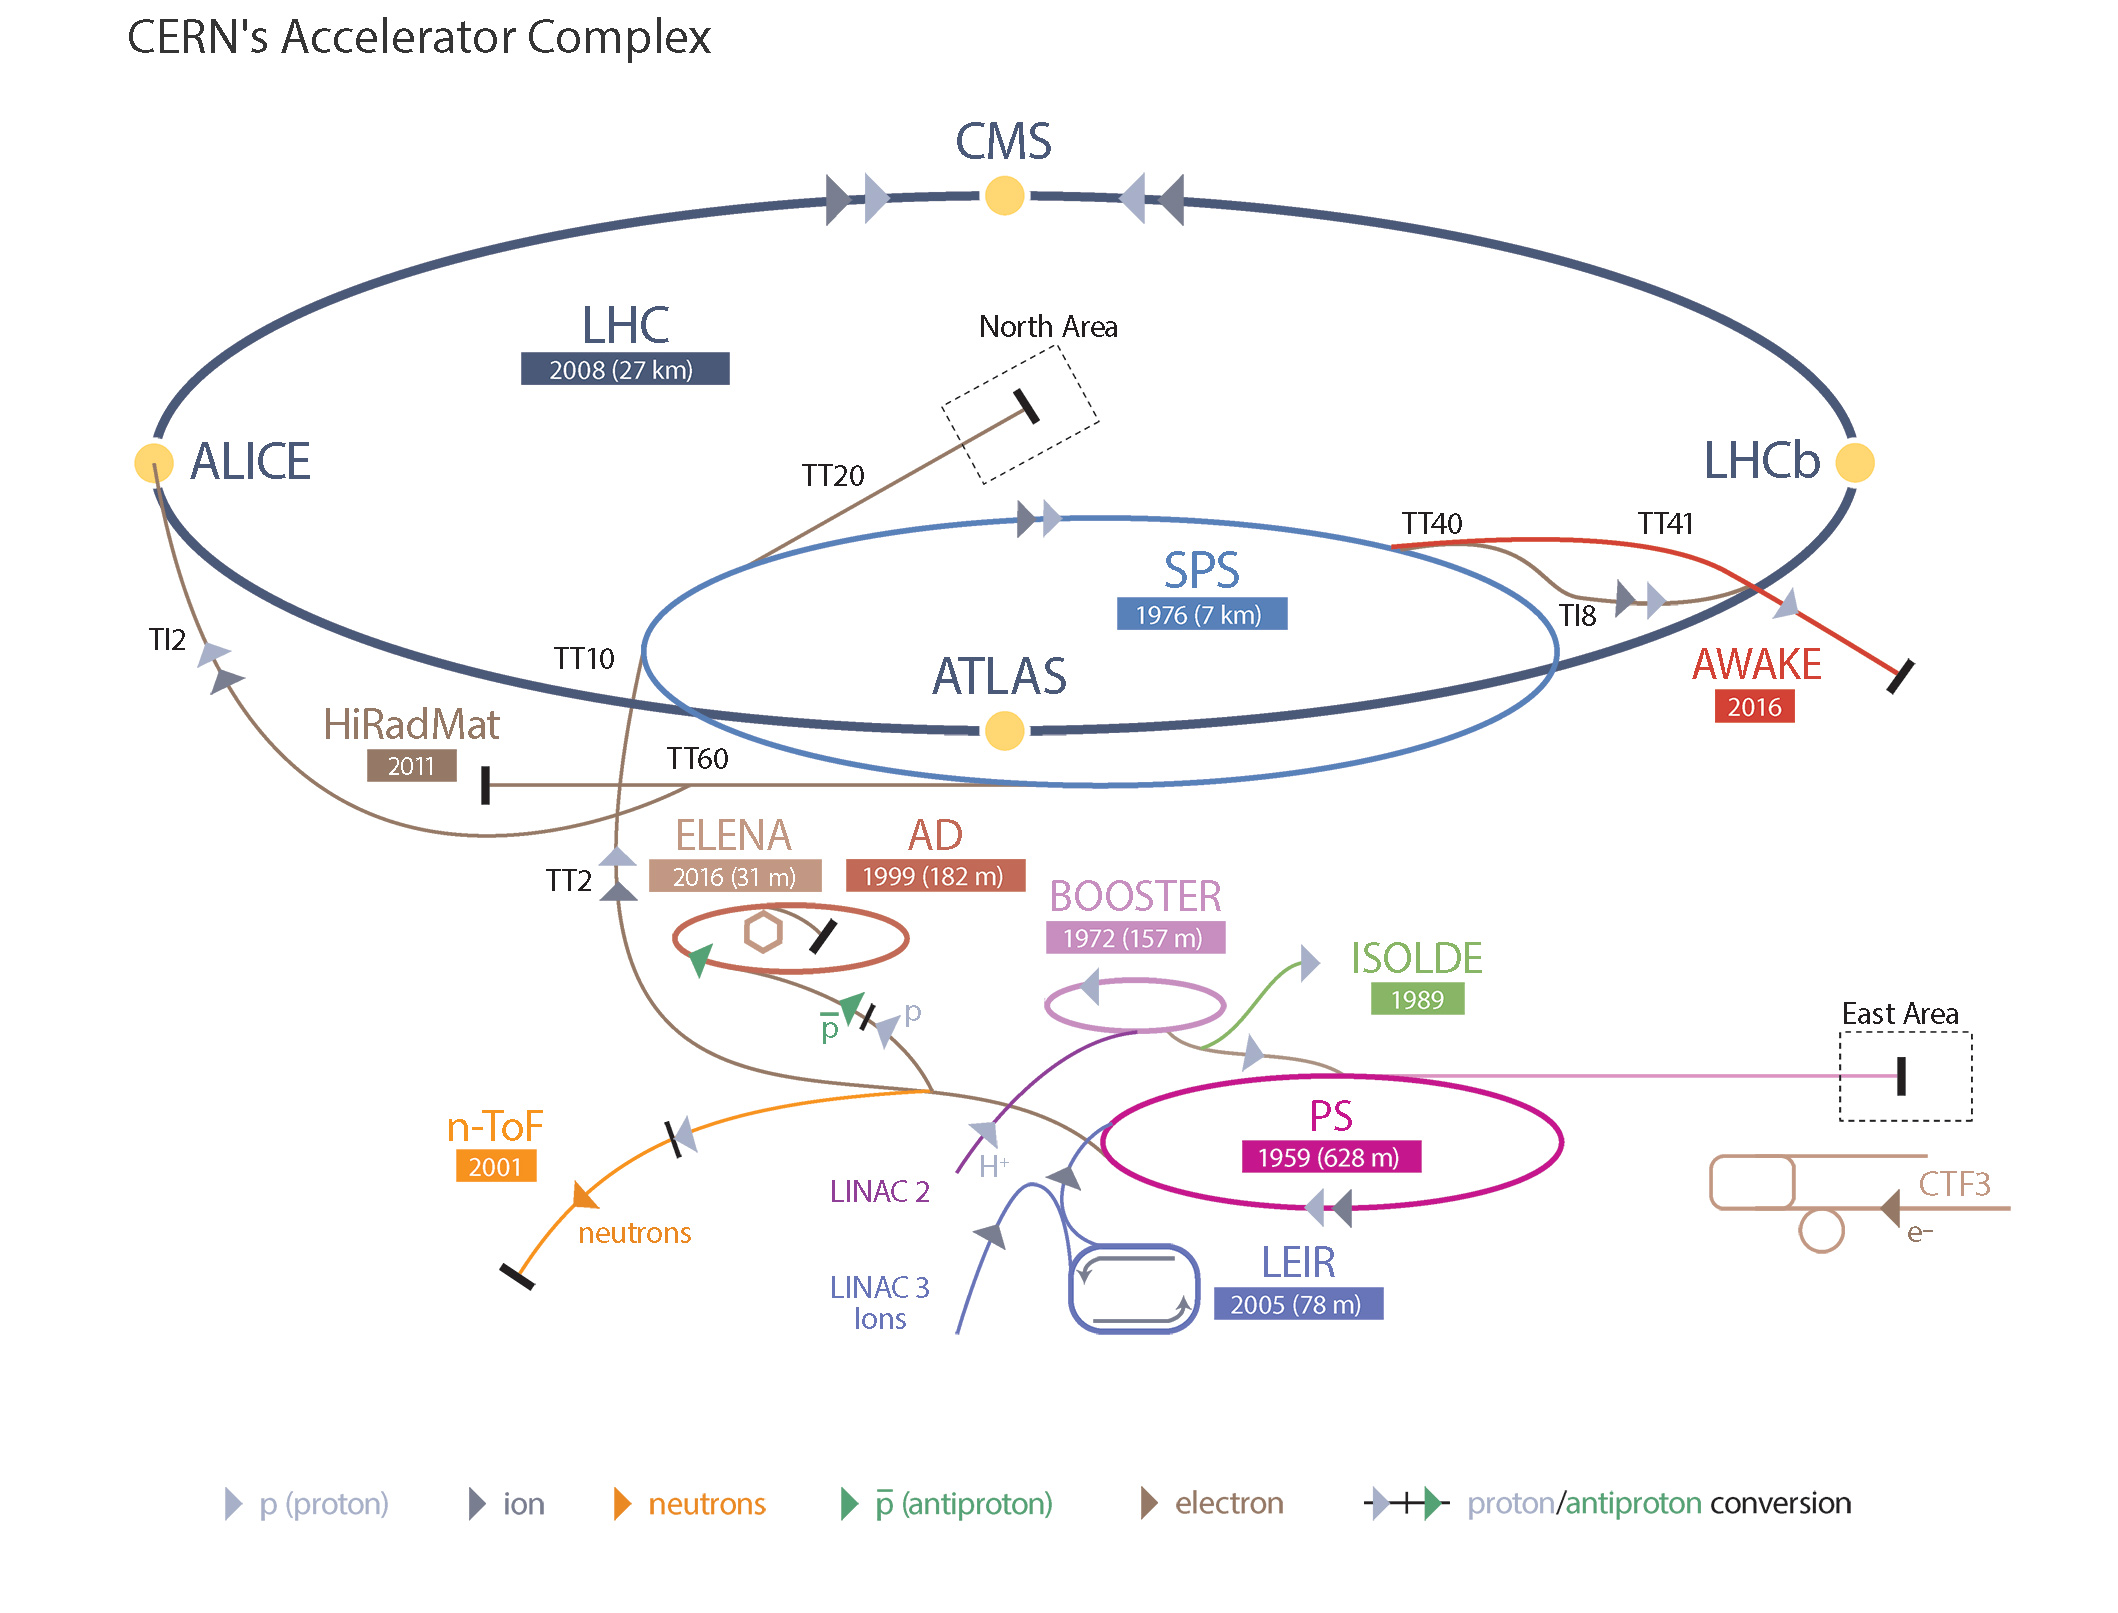
\includegraphics[width=0.8\textwidth]{figures/chapter2/cern_accelerator_complex2}
        \caption{
            Illustration of the various beamlines, accelerator and storage rings, and experimental
            points that the CERN accelerator complex is home to.
            The protons that circulate through the LHC, and that are eventually made to collide inside
            the ATLAS detector, follow the path: Linac 2 $\rightarrow$ Booster $\rightarrow$ Proton Synchotron (PS)
            $\rightarrow$ Super Proton Synchotron (SPS) $\rightarrow$ LHC.
            Figure taken from Ref.~\cite{CERNAcceleratorComplex}.
        }
        \label{fig:cern_complex}
    \end{center}
\end{figure}


%%%%%%%%%%%%%%%%%%%%%%%%%%%%%%%%%%%%%%%%%%%%%%%%%%%%%%%%%%%%%%%%%%%
%%%%%%%%%%%%%%%%%%%%%%%%%%%%%%%%%%%%%%%%%%%%%%%%%%%%%%%%%%%%%%%%%%%
% sub-section describing the LHC
%%%%%%%%%%%%%%%%%%%%%%%%%%%%%%%%%%%%%%%%%%%%%%%%%%%%%%%%%%%%%%%%%%%
%%%%%%%%%%%%%%%%%%%%%%%%%%%%%%%%%%%%%%%%%%%%%%%%%%%%%%%%%%%%%%%%%%%
\section{The Large Hadron Collider}
\label{sec:lhc}

The LHC~\cite{LHCMachine} is a circular particle accelerator, with a 27~kilometer circumference,
located at an average distance of 100 meters beneath the surface of the Earth.
It is nominally used for proton-proton ($pp$) collisions, wherein two counter-rotating
beams of protons are made to collide head-on at specific interaction points (IP) along the 27~kilometer
ring, but can also be run in heavy-ion configurations wherein proton-lead ($p$-Pb) or lead-lead (Pb-Pb)
collisions take place.\footnote{The specific lead (Pb) species used in collisions is $^{208}_{82}$Pb.}\footnote{More rarely, the LHC can also be used to circulate gold (Au) ions.
There are even plans to have proton-oxygen ($p$-O) runs in the future, which will allow
for the LHC experiments to provide research that potentially complements dark matter research
based on cosmic-ray air showers.}
The $pp$ collisions take priority over those of the heavy-ions, with the collisions each year
consisting of only a few weeks in the winter for the heavy-ion configurations and typically
six to seven months for the $pp$ configuration. The LHC is designed to accelerate protons to a
center-of-mass energy of $\sqrt{s} = 14\,\TeV$.

\subsection{Machine Design and Layout}
\label{sec:lhc_layout}

\paragraph{Machine Composition} \mbox{} \\
\label{sec:dipole}
The LHC was planned as the successor to the Large Electron Positron (LEP) collider~\cite{LEPI,LEPII}, which was in operation
between the years of 1989 to 2000. LEP is still the most powerful lepton collider to date, having maximal electron-positron
center-of-mass collision energies of 209\,\GeV.
After LEP, the particle physics community knew that the next collider at CERN needed to have $\mathcal{O}(10)$\,\TeV~collision
energies; either to be able to probe from all angles any new physics discovered at LEP and/or the Tevatron~\cite{TevatronDesignI}, or
to provide the necessary power to search for still-elusive hints of BSM physics. At the very least,
given a non-discovery of the Higgs boson at LEP and the Tevatron, the community would need a discovery machine powerful enough
to produce electroweak-scale Higgs bosons and an $\mathcal{O}(10)$ \TeV~hadron collider --- as we now know --- is sufficient for this job.


In order to increase center-of-mass collisions energies, collider designs can take two routes: they can
either increase in size, that is, have larger circumferences (radii), or they can increase the strength of the magnetic
fields used to keep the circulating charged particles in orbit. This can be seen by first considering the expression
for the relativistic cyclotron frequency, $\omega$, of a particle moving in a circular orbit,
\begin{align}
    \omega = \frac{qB}{\gamma m},
    \label{eq:rel_cyclotron}
\end{align}
where $m$ is the particle's rest mass, $B$ is the magnitude of the magnetic field experienced by the
particle, $q$ is the particle's electric charge, and $\gamma$ is the relativistic Lorentz factor, $\gamma = \sqrt{1 - \beta^2} = \sqrt{1 - (v/c)^2}$,
with $v$ the particle's velocity and $c$ the speed of light.
Using Eqn.~\ref{eq:rel_cyclotron}, it can be seen that a particle of higher energy confined to a fixed
circular orbit necessarily has a higher angular velocity by relating the particle's angular
velocity to its kinetic energy:
%A particle of higher energy confined
%to a fixed circular orbit necessarily has a higher
%angular velocity, which can be seen by the expression relating the above angular velocity of the particle to its kinetic energy:
\begin{align}
    E_{\text{kin}} \propto m v^2 = m(\omega R)^2 = \frac{q^2 B^2 R^2}{m \gamma^2}.
    \label{eq:kinetic_energy_gen}
\end{align}
In planning the construction of the LHC, the costs in civil engineering and real-estate works that would
be required to construct a larger tunnel in which to house the LHC ring (increasing $R$) far outweighed
the costs of research into and development of magnet systems strong enough to bend the
multi-\TeV~particles along the beam orbit prescribed by the already-existing LEP tunnel (increasing $B$).
The desired center-of-mass collision energy of $\mathcal{O}(10)$\,\TeV, the fact that the LHC would be a hadron (proton)
collider, and the fact that the LHC would be using the existing LEP tunnel dictate the required magnetic
field strength needed to keep the protons in stable orbits at the LHC. This
is seen by using Eqn.~\ref{eq:kinetic_energy_gen}, solving for $B$, and comparing the LHC and LEP
design parameters,
\begin{align}
    \hspace{-0.4cm}
    \frac{B^2_{\text{LHC}}}{B^2_\text{LEP}} &= \frac{ (E_{\text{LHC}} m_{\text{LHC}} \gamma_{\text{LHC}}^2) / (q_{\text{LHC}}^2 R_{\text{LHC}}^2)  } { (E_{\text{LEP}} m_{\text{LEP}} \gamma_{\text{LEP}}^2) / (q_{\text{LEP}}^2 R_{\text{LEP}}^2) } \label{eq:lhc_mag_field} \\
        &= (E_{\text{LHC}} / E_{\text{LEP}}) \times (m_{\text{LHC}} / m_{\text{LEP}}) \times (\gamma_{\text{LHC}}^2 / \gamma_{\text{LEP}}^2) \times (q_{\text{LEP}}^2 / q_{\text{LHC}}^2) \times (R_{\text{LEP}}^2 / R_{\text{LHC}}^2) \notag \\
        &\approx ( 1\,\TeV~/0.2\,\TeV) \times (m_p/ m_e) \times (1) \times (1) \times (1) \notag \\
        &\approx 10^4 \notag,
\end{align}
which shows that the strength of the LHC bending magnets must be on the order of $100\times$
the strength of those used at LEP. The magnetic fields experienced by the electron and positron beams
at LEP were 0.22 Tesla. By Eqn.~\ref{eq:lhc_mag_field}, the LHC bending magnets should achieve magnetic field
strengths on the order of 10 Tesla in order to achieve the desired collision energies.
The maximum achievable magnetic field of conventional ferrormagnets is about 2 Tesla.
To meet the $\sqrt{s}\approx$10\,\TeV~design goal, the magnet system used by the LHC to confine the protons to their circular orbits
must then be composed of \textit{superconducting} electromagnets. %\footnote{Note that even though
%the main dipole bending magnets at LEP were not superconducting, its focusing quadrupole magnets
%\textit{were} superconducting. There are simply fewer quadrupole magnets, as compared to the number of
%dipole magnets, required for a particle collider.}
The entire magnet system of LEP was therefore removed and replaced with superconducting
niobium-titanium (Nb-Ti) alloy based electromagnets which are superconducting
at temperatures below $10$\,K.
%All of the magnets at the LHC are constructed with
%current carrying elements composed of a niobium-titanium (Nb-Ti) alloy that becomes superconducting
%for temperatures below $10$\,K.
To reach temperatures below this $10$\,K threshold, the LHC magnets
are housed in cryostats that allow for the Nb-Ti elements to be fully submerged in a bath
of superfluid Helium at a temperature of $1.9$\,K~\cite{Casas:1992nf}.
In total, the LHC contains more than 120 tonnes of superfluid Helium.
It goes without saying that there is a significant amount of resources and person power at CERN devoted to the refrigeration and cryogenics
systems that are required for the LHC to run.

Additionally, the fact that LEP was a \textit{particle-antiparticle} collider meant that the counter-rotating
beams could be made to occupy a single ring: the same magnetic field could produce counter-rotating beams of
electrons and positrons within the same beam pipe.\footnote{The electrons and positrons at LEP were vertically separated
within the beam pipe by electrostatic separators placed throughout the LEP ring. Turning off these separators
is, to first approximation, how the LEP operators would get the electrically-attracting electrons and positrons to collide.}
As a result, the LEP beam tunnel was constructed with only a single ring in mind and is relatively narrow: the LEP tunnel,
and therefore LHC tunnel, is only $\approx$3.7\,m wide on average.
As the LHC is a \textit{particle-particle} collider, it necessarily requires \textit{two} magnetic fields
of opposing polarity to circulate one of its beams in the clockwise direction and the other in the
counter-clockwise direction.
Given the limited space in the tunnel, however, it is not possible to house two separate rings
of superconducting bending magnets with all of the services that they require \textit{in addition} to the requisite
minimal space needed for personnel and maintenence access.
This forced the need of the so-called `2-in-1' design of the main bending magnets of the LHC, wherein the two
beam pipes are housed in the same cryostat in which the counter-rotating beams are held in their
respective orbits by coupled magnetic fields.
An illustration of this now-iconic design of the LHC bending (dipole) magnets and surrounding cryostat and containment structure is illustrated in Figure~\ref{fig:lhc_dipole_xsec}.
Each of the 15\,meter long superconducting dipole electromagnets of the LHC responsible for constraining the protons to their circular
orbits has currents of $11850$\,Amperes flowing through it and achieves magnetic field strengths of $8.33$\,Tesla.

\begin{figure}[!htb]
    \begin{center}
        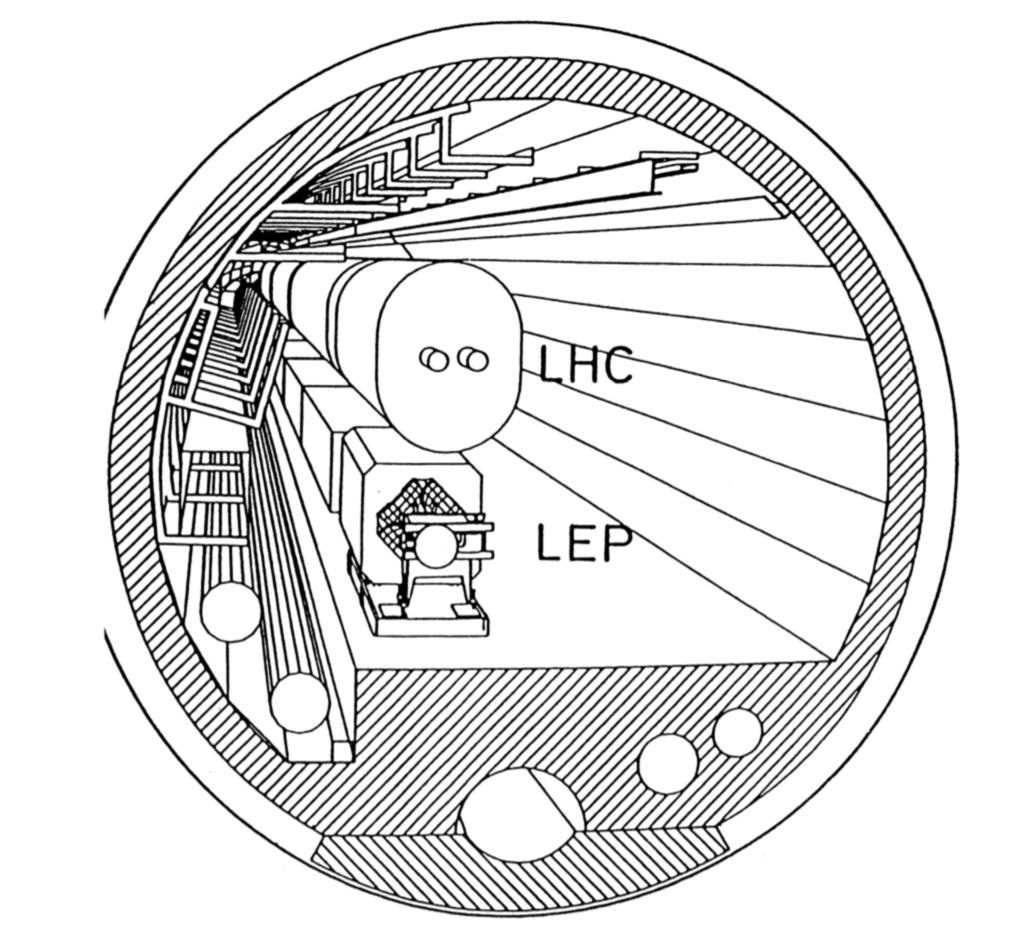
\includegraphics[width=0.43\textwidth]{figures/chapter2/lhc_lep_dipole_comp}
        \includegraphics[width=0.50\textwidth]{figures/chapter2/lhc_lep_dipole_comp_person}
        \caption{
            \textit{Left}: Illustration comparing the size of a `2-in-1' LHC dipole configuration to the
                LEP dipole and how they fit inside of the LEP/LHC tunnel. Note that prior to LHC operation,
                the LEP magnets will have been removed: the two are shown side-by-side for comparison purposes only.
            \textit{Right}: Cross-sectional view of the LEP/LHC tunnel with a comparison of the LHC `2-in-1' dipole
                on top of the LEP dipole. An illustration of an average size person is shown
                for scale. Also shown is the service crane in use, to give an idea of the size required
                for potential maintenance access. Clearly, two single-bore, superconducting rings each similar in size
                to the LEP dipole would not fit comfortably in the tunnel. The LHC `2-in-1' design fits
                in nearly the same area as the LEP dipoles while additionally being able to contain both
                particle beams.
                Figures are taken from Ref.~\cite{ECFALHCinLEP}.
        }
        \label{fig:lhc_lep_dipole_comp}
    \end{center}
\end{figure}

\begin{figure}[!htb]
    \begin{center}
        \begin{minipage}{\textwidth}
        \includegraphics[width=0.59\textwidth]{figures/chapter2/lhc_dipole_fig3p3}
        \raisebox{0.5cm}{\includegraphics[width=0.4\textwidth]{figures/chapter2/dipole_magnetic_field_lines}}
        \end{minipage}
        \caption{
            \textit{Left}: Cross-sectional view of an LHC dipole bending magnet, with relevant parts indicated.
            The protons orbit inside of the beam pipes, each of which has a diameter of roughly $3$\,cm.
            It is interesting to note that the non-magnetic steel collars (in green) are of critical import
            to the success of the magnet systems. They are required
            to prevent the dipole structure from being deformed or torn apart due to the intense magnetic forces
            tending to push the two beam-pipes apart as a result of their counter-rotating electromagnetic currents.
            These forces amount to about 400 tonnes per meter of dipole when in full operation --- almost equivalent in magnitude
            to the weight of a Boeing 747.
            \textit{Right}: Magnetic field lines of the coupled dipole fields that bend the counter-rotating proton beams
            and keep them in their circular orbits around the LHC ring.
        }
        \label{fig:lhc_dipole_xsec}
    \end{center}
\end{figure}


%\FloatBarrier
\paragraph{Connecting the Dots} \mbox{} \\
The LHC is essentially a chain of superconducting magnets of the type described in the previous paragraphs, where
the the bending (dipole) magnets critical to the LHC design were introduced.
%There are additional
%types of magnets that produce fields of higher multipole moments which, in the case of the quadrupole magnets, are
%necessary for beam \textit{beam focusing}. Conceptually they are very similar to the dipoles and are 
The chain is laid in a double-octagonal structure, illustrated in Figure~\ref{fig:lhc_layout}. There are eight
octants, at the center of which the LHC ring is straight and does not curve.
The LHC curvature occurs at the
boundaries of each of the octants and is primarily made up of bending (dipole) magnets.
The straight sections are where the interaction regions are located and are referred
to as `Points', numbered 1 to 8.
Points 1, 2, 5, and 8 are where the four large LHC experiments are located.
Points 1 and 5 are home to the services and underground areas
of the general purpose experiments, ATLAS and CMS, respectively.
The underground experimental caverns associated with Point 1 and 5 were not present for LEP and
had to be constructed after LEP was retired in 2000.
Figure~\ref{fig:p1} provides an illustration of how the surface and underground
areas are situated at Point 1.
Points 2 and 8 host the services and underground areas of the ALICE and LHCb experiments, respectively.
At these Points, Points 1, 2, 5, and 8, the counter-rotating beams are
made to collide. The remaining Points, Points 3, 4, 6, and 7, are host to various beam `services'
necessary for the operation of the LHC.
Point 3 and 7 host the beam betatron and momentum cleaning (`beam collimation') systems, respectively.
Point 4 hosts the superconducting radio-frequency (RF) systems which accelerate the beams to
their nominal collision energies.
Point 6 is the location of the beam-abort system --- the so-called `beam dump' --- where
the LHC beams may be removed very quickly from the LHC ring by using \textit{kicker} magnets~\cite{LHCDesignI}
that divert the beams out of the LHC ring in a safe manner. The beams may be dumped
if the LHC wishes to refill with protons (or heavy-ions) and needs to remove any
remnants of the previous fill, in case of beam instabilities observed in the LHC ring,
or if one of the experiments signals the need for a beam dump (in case of
beam stability or detector issues observed at the associated IP).

\begin{figure}[!htb]
    \begin{center}
        \includegraphics[width=0.8\textwidth]{figures/chapter2/lhc_layout}
        \caption{
            Layout of the LHC and its two counter-rotating beams. Beam 1 is in blue and rotates
            counter-clockwise. Beam 2 is in red and rotates clock-wise.
            At the center of each octant is a straight section which houses
            the experimental caverns or LHC beam facilities.
            At the boundaries of each octant are located the curved sections.
            Figure taken from Figure 2.1 of Ref.~\cite{LHCMachine}.
            {\color{red}{Somewhere $\beta$ should be described -- betatron function}}
        }
        \label{fig:lhc_layout}
    \end{center}
\end{figure}

\begin{figure}[!htb]
    \begin{center}
        \includegraphics[width=0.75\textwidth]{figures/chapter2/point1_illustration}
        \caption{
            Diagram showing the surface buildings and services and underground areas of Point 1, where
            the ATLAS experiment is located. The LHC ring can be seen at the bottom,
            with its directions indicated by the `VERS PT8 (2)' arrows pointing
            towards Point 8 (2).
            The experimental cavern in which the ATLAS detector sits is UX15.
            The control room for the ATLAS experiment, whereat operators can monitor and
            control the state of the ATLAS detector, is located 100\,m above
            UX15 in the building SCX1.
            Figure taken from Figure 10.1 of Ref.~\cite{LHCDesignII}.
        }
        \label{fig:p1}
    \end{center}
\end{figure}

%\FloatBarrier
\subsection{Injection Chain and Bunch Structure}
\label{sec:lhc_injection}

We now have an idea of how the proton beams relevant to the work
in this thesis are made to circulate in the LHC ring.
In this section we will briefly describe the initial source of the protons and how
they are introduced into the LHC ring.
The LHC relies on a series of pre-acceleration steps that bring the initial
low-energy protons to energies sufficient enough to begin their journey through the LHC.
The sum-total of these steps is referred to as the LHC \textit{injection chain}~\cite{LHCDesignIII}.
The components of the LHC injection chain form the heart of the CERN accelerator
complex illustrated in Figure~\ref{fig:cern_complex}.
For $pp$ collisions in the LHC, the protons are initially sourced from Hydrogen atoms that are released
at the start of Linac 2.
The Hydrogen atoms are immediately stripped of their electrons after passing through
the \textit{duoplasmatron} ion source~\cite{Duoplasma}.
The protons are then passed through Linac 2, a linear accelerator, which accelerates
the protons to $50$\,\MeV.
They then enter the Proton Synchotron Booster (PSB), a circular storage ring
composed of four stacked rings, which accelerates the protons to $1.4\,\GeV$.
The PSB injects the protons into the Proton Synchotron (PS) which accelerates
them to $25$\,\GeV.
The Super Proton Synchotron (SPS) receives the protons from the PS and
accelerates them to $450$\,\GeV.
At this point the protons have sufficient energy to be injected into the LHC.
There are two injection points into the LHC since, up until this stage,
the protons are circulating in the same direction: one injection point sends
protons into the counter-clockwise beamline of the LHC, and the other
into the clockwise beamline.
Until all of the protons from a single \textit{fill} make their way into
the LHC, they will circulate at the injection energy of $450$\,\GeV.
After the filling completes\footnote{A standard LHC fill takes on the order of 4 minutes per
ring.}, the superconducting RF cavities located at Point 4 will begin to accelerate the protons
to their final collision energies.\footnote{If all goes smoothly, this acceleration stage takes roughly 20 minutes.}
The acceleration is achieved by increasing the frequency of the RF oscillations; however,
given that a $450$\,\GeV~proton is already ultra-relativistic, the adjustment of the frequency
needed to get to the collision energies is not large.

The proton beams circulating the LHC are not a continuous stream of protons; rather,
they are grouped into what are referred to as \textit{bunches}.
The protons arrive at the LHC in these bunches which are initially prepared
in the smaller machines that make up the LHC injection chain and then are
kept in their final \textit{bunch structure} by the RF cavities.
The accelerating RF cavities provide an accelerating electromagnetic field
that oscillates longitudinally. The bunches, each composed of roughly $10^{11}$ protons,
are then made to oscillate longitudinally in so-called \textit{synchotron oscillations}
around the central node of the RF oscillation as they circulate through the LHC ring.
The proton bunches are then effectively `shaped' by the oscillating RF field: protons in a bunch
lagging behind or that are ahead of those particles at the center of the bunches
will be accelerated or decelerated accordingly so as to be pushed back into the center of the bunch.
The LHC RF cavities have an oscillation frequency of $400$\,MHz which
defines the boundaries in which proton bunches can lie. These boundaries are
called \textit{RF buckets} and, along with
the circumference of the LHC, dictate the number of proton bunches that
can potentially fit in the LHC.
The relationship between the RF oscillations and the RF bucket and bunch structure
is illustrated in Figure~\ref{fig:lhc_bunch}.
In total, approximately 35640 RF buckets exist when the LHC is in operation.
Not all buckets contain proton bunches, however.
In fact, at the time of the writing of the present thesis,
RF buckets filled with proton bunches have a minimal separation of 10 RF buckets, meaning
that following an RF bucket containing a proton bunch there is at least 9 unfilled RF buckets.
This corresponds to a minimal
time between proton bunches --- the \textit{bunch spacing} --- of $25$\,nanoseconds.
At the time of the present thesis, the operating conditions of the LHC maximally
allow for 2808 $25$\,ns-spaced bunches.\footnote{
The number of allowed bunches is significantly lower than the 35640 RF buckets with $25$\,ns
bunch-spacing potentially allow for. This is due, in part, to the non-trivial bunch-structure
typically employed but also in large part to the fact that there is a rather long \textit{abort gap}
in the LHC ring where no filled RF buckets exist.
The abort gap is a number of continuous unfilled RF buckets that allows the ramp up of the kicker
magnets used for the beam dump to occur in the absence of filled buckets.
In this way, the kicker magnet ramp up does not disturb the structure of the circulating proton beams.
Only after this ramp up is finished should the kicker magnets disturb the beams.
}
The bunch-spacing and overall bunch structure of an LHC fill is not only decided
by the operators of the LHC but also by what the detectors at Points 1,2,5, and 8
can tolerate. This is because shorter bunch spacing means higher intensity and multiplicity
of collisions occuring at each of these IP. A $25$\,nanosecond bunch spacing
corresponds to a maximal $pp$ collision rate of $40$\,MHz. The detectors at each
of the IP have been designed with this collision rate in mind and anything
higher may push them beyond their design limits.

\begin{figure}[!htb]
    \begin{center}
        \includegraphics[width=0.5\textwidth]{figures/chapter2/lhc_bunch}
        \caption{
            Illustration of the particle bunch structure in a particle collider such as the LHC.
            The particles are accelerated by radio-frequency (RF) oscillations whose
            amplitude is illustrated in the upper plot.
            The RF bucket's boundary, illustrated in the lower plot, is defined by a full period of the RF oscillation
            and the particle bunch formation, depicted in grey, occurs at the central node of the oscillation.
            The area occupied by the particle bunch is related to the beam's longitudinal
            \textit{emittance}.
        }
        \label{fig:lhc_bunch}
    \end{center}
\end{figure}

\subsection{The Concept of Luminosity}
\label{sec:lhc_luminosity}

In designing a particle collider, the collision energy is not the only important parameter.
Equally important is the value of the instantaneous \textit{luminosity}
that can be achieved by the collider.
An expression for the instantaneous luminosity, $\mathcal{L}$, is given by,
\begin{align}
    \mathcal{L} = \frac{N^2 n_b f}{4 \pi \sigma_x \sigma_y} \cdot S,
    \label{eq:luminosity}
\end{align}
where $N$ is the number of particles per bunch, $n_b$ is the number of colliding bunches,
$f$ is the bunch revolution frequency, $\sigma_{x,y}$ are the transverse beam widths in the
Gaussian approximation, and $S$ is a reduction factor that accounts for geometric factors
such as the non-zero crossing-angle of the colliding beams~\cite{LHCDesignIII,LumiConcept}.
The instantaneous luminosity, $\mathcal{L}$, can be seen by Eqn.~\ref{eq:luminosity}
to have units of cm$^{-2}$s$^{-1}$ and can be conceptually thought of as the
outgoing flux of particles per unit area and time after a bunch crossing in which successful $pp$
collisions occur.
The LHC is designed to deliver collisions to the high luminosity IP (Fig.~\ref{fig:lhc_layout})
at $\mathcal{L} = 10^{34}$\,cm$^{-2}$s$^{-1}$.
Accurate knowledge of $\mathcal{L}$ is of the utmost importance for collider design and operation.
Not only does it parametrise the potential collision rate once the collider beam and bunch
structure are decided, but it allows for the accurate prediction of the number
of collision events, $N_{\text{proc}}$, associated with a particular physics process
with cross-section $\sigma_{\text{proc}}$,
\begin{align}
    N_{\text{proc}} = \sigma_{\text{proc}} \int \mathcal{L}\, \mathrm{d}t \equiv \sigma_{\text{proc}} \cdot L,
    \label{eq:n_exp_lumi}
\end{align}
where $L$ is referred to as the \textit{integrated luminosity} and has units of cm$^{-2}$.
A common unit for integrated luminosity is the \textit{barn}, with symbol `b': one barn is defined as $10^{-24}$\,cm$^{-2}$.
The datasets collected by the LHC experiments are such that the \textit{femtobarn} (fb), $10^{-39}$\,cm$^{-2}$, is relevant.

\subsection{Operation of the Large Hadron Collider}
\label{sec:lhc_operation}

The LHC has been in stable operation since 2009.
It operates in so-called \textit{runs}: multi-year periods of roughly continuous
data-taking.
As CERN shuts down during the winter months, each run is segmented each year
with a several month long shutdown in the winter with a ramp-up period in the spring.
During these shorter shutdowns, maintenance and upgrades may also take place.
In between a given run there is a multi-year break, a \textit{long shutdown},
in which large(er)-scale maintenance and upgrades of both the LHC and the experiments can take place.
At the time of writing, there has so far been two runs of the LHC, Run-I and Run-II.
Run-I took place during the years 2009--2012 and Run-II during 2015--2018.
The integrated luminosities for each of the data taking years between Run-I and Run-II
is shown in Fig.~\ref{fig:int_lumi_multiyear}.
The data relevant to the work presented in this thesis were collected in both
Run-I and Run-II of the LHC, specifically that data collected in the years 2012--2018.
The luminosities, instantaneous and integrated, as well as the center-of-mass collision energies, $\sqrt{s}$, for these data-taking periods are
shown in Table~\ref{tab:lumi_tab}.
Also shown in Table~\ref{tab:lumi_tab} are the average values of the mean number of interactions per bunch
crossing, $\langle \mu \rangle$, observed during each data-taking year. The quantity $\langle \mu \rangle$
is related to the amount of \textit{pileup} observed during data-taking. Pileup is caused
by overlapping $pp$ interactions within the same (\textit{in-time} pileup) or neighboring (\textit{out-of-time} pileup)
bunch-crossing(s) at the interaction point. The pileup scales with the instantaneous luminosity.
Distributions of $\langle \mu \rangle$ are shown in Fig.~\ref{fig:int_lumi_multiyear} for
the Run-II data-taking period.


\begin{table}[!htb]
    \begin{center}
        \begin{tabular}{l | c | c c c c }
        \hline
        \hline
        & \textbf{Run-I} & \multicolumn{4}{c}{\textbf{Run-II}} \\
        \hline
        Year & 2012 & 2015 & 2016 & 2017 & 2018 \\
        \hline
        Collision energy, $\sqrt{s}$ [TeV] & 8 & \multicolumn{4}{c}{13} \\
        Peak Luminosity, $\mathcal{L}$ [cm$^{-2}$s$^{-1}$] ($\times10^{34}$) & $0.77$ & $0.5$ & $1.4$ & $2.1$ & $2.1$ \\ 
        Integrated Luminosity, $L$ [fb$^{-1}$] & 20.2 & 3.2 & 33.0 & 44.3 & 59.9 \\
        Mean number of of interactions & & & & & \\
        \hspace{1.7cm} per bunch crossing, $\langle \mu \rangle$ & 20.7 & 13.4 & 25.1 & 37.8 & 36.1 \\
        \hline
        \hline
        \end{tabular}
        \caption{
            Summary parameters for the data-taking periods relevant to the work
            presented in this thesis. The integrated luminosity is that relevant
            to performing physics analysis and potentially differs with respect to
            the total integrated luminosity delivered to ATLAS by the LHC (Fig.~\ref{fig:int_lumi_multiyear}) due to
            the application of strict quality criteria on the data prior to its use
            in physics analyses.
        }
        \label{tab:lumi_tab}
    \end{center}
\end{table}

\begin{figure}[!htb]
    \begin{center}
        \includegraphics[width=0.49\textwidth]{figures/chapter2/int_lumi_multiyear}
        \includegraphics[width=0.49\textwidth]{figures/chapter2/mu_run2}
        \caption{
            \textit{Left}: The ATLAS integrated luminosity during the data-taking years 2011--2018.
            \textit{Right}: The observed average number of $pp$ interactions per bunch-crossing, $\langle \mu \rangle$,
                observed by ATLAS during the Run-II data-taking years, 2015--2018.
        }
        \label{fig:int_lumi_multiyear}
    \end{center}
\end{figure}

\FloatBarrier

%%%%%%%%%%%%%%%%%%%%%%%%%%%%%%%%%%%%%%%%%%%%%%%%%%%%%%%%%%%%%%%%%%%
%%%%%%%%%%%%%%%%%%%%%%%%%%%%%%%%%%%%%%%%%%%%%%%%%%%%%%%%%%%%%%%%%%%
% sub-section describing ATLAS
%%%%%%%%%%%%%%%%%%%%%%%%%%%%%%%%%%%%%%%%%%%%%%%%%%%%%%%%%%%%%%%%%%%
%%%%%%%%%%%%%%%%%%%%%%%%%%%%%%%%%%%%%%%%%%%%%%%%%%%%%%%%%%%%%%%%%%%
\section{The ATLAS Detector}
\label{sec:atlas}

In this section we will extend our focus to the ATLAS detector, the general purpose
particle detector located at Point 1 of the LHC ring (see Figure~\ref{fig:p1}).
Roughly cylindrical in shape, coaxial with the beam-pipe,
the ATLAS detector is 44\,m long and 25\,m tall.
It is by far the largest such detector ever built and,
generally, is the largest and most complex device ever constructed.
Being general purpose in scope, the ATLAS detector is hermetic and has
nearly $4\pi$ radians of solid angle coverage around the $pp$ collision
point. 
Such detectors are commonly designed to have various subsystems --- \textit{subdetectors} ---
which are designed for the identification of specific types of particles
and interactions.
They tend to be layered about the interaction point and cylindrically symmetric
since the $pp$ interactions taking place within the detector have no preferred
direction in the plane transverse to the direction in which the proton beams
are travelling.
A view of the ATLAS detector and its subdectors is provided by Figure~\ref{fig:atlas_cutaway}.
In the following we will briefly describe each subsystem in turn, describing
first the detectors located nearer to the $pp$ collision and proceeding outwards.

\subsection{The ATLAS Coordinate System}
\label{sec:atlas_coordinate_system}

The ATLAS detector uses a right-handed coordinate system with the origin located at
the geometric center of the detector.
The $x$-axis points to the center of the LHC ring, the $y$-axis points upwards
and away from the center of the Earth, and the $z$-axis is along the beam-pipe.
The side associated with positive (negative) $z$
is referred to as the `A' (`C') side of the detector.\footnote{`A' for `airport',
since this is the side pointing towards Geneva International Airport, and
`C' for either `Crozet' or `Charly's', depending on who you ask, since this is the side
pointing towards the town of Crozet and/or Charly's Pub in the town of Saint-Genis-Pouilly.}
Due to its cylindrical symmetry, ATLAS also uses the cylindrical coordinates, $(r,\phi, z)$,
with $\phi$ the azimuthal angle about the $z$-axis and having $\phi = 0$ along the positve $x$-axis.
The spherical polar angle, $\theta$, is defined with respect to the $z$-axis, having
$\theta = 0$ parallel to the beam-pipe and $\theta = \pi/2$ in the $xy$-plane transverse
to the beam-pipe.
The pseudorapidity, $\eta$, is commonly used when describing systems of particles or locations within
the detector and is defined as $\eta = - \ln \left[ \tan \left( \theta / 2 \right) \right ]$.
The relationship between pseudorapidity and polar angle is illustrated in Figure~\ref{fig:eta_desc}.
Large (small) values of $\eta$ correspond to the \textit{forward} (\textit{central}) region of the detector.
The rapidity, $y$, is related to $\eta$ and is defined as $y = \frac{1}{2} \ln \left[ (E+p_z) / (E-p_z) \right]$.
The pseudorapidity of a particle traversing the detector is equal to its rapidity if
the particle is massless or ultra-relativistic; otherwise, they are different.
The comparison between a particle's pseudorapidity and rapidity is illustrated in
Figure~\ref{fig:eta_desc}.
The coordinates used to describe systems of particles are typically described by their
four-momenta: $(p_x, p_y, p_z)$ or, equivalently, $(\pT, \eta, \phi)$.
A distance metric commonly used to describe the distance between two systems of particles
in the detector is $\Delta R = \sqrt{ (\Delta \eta)^2 + (\Delta \phi)^2 }$. The
$\Delta R$ quantity using $y$ instead of $\eta$ is also sometimes used and will be
indicated by $\Delta R_y$.

\begin{figure}[!htb]
    \begin{center}
        \raisebox{1.5cm}{\includegraphics[width=0.35\textwidth]{figures/chapter2/eta_vs_polar}}
        \includegraphics[width=0.55\textwidth]{figures/chapter2/eta_vs_rap}
        \caption{
            \textit{Left}: Illustration of the relationship between the pseudorapidity, $\eta$,
                and polar angle, $\theta$, defined as the angle with respect to the beam-axis ($z$-axis).
            \textit{Right}: Distribution of the ratio of a particle's pseudorapidity to its rapidity, $\eta$/$y$,
                as a function of its pseudorapidity ($y$-axis) and the ratio of its mass to its transverse momentum, \pT~($x$-axis).
        }
        \label{fig:eta_desc}
    \end{center}
\end{figure}


\begin{figure}[!htb]
    \begin{center}
        \includegraphics[width=0.95\textwidth]{figures/chapter2/atlas_cutaway}
        \caption{
            Cut-away view of the ATLAS detector with sub-systems indicated.
            Shown for comparison are figures of average-height humans standing
            at the feet of the detector and standing on the forward shielding
            between the big wheels of the forward muon system.
        }
        \label{fig:atlas_cutaway}
    \end{center}
\end{figure}


\begin{figure}[!htb]
    \begin{center}
        \includegraphics[width=0.95\textwidth]{figures/chapter2/atlas_magnet_system}
        \caption{
            A view of the ATLAS magnet system. Shown are the 2\,T solenoid magnet
            in green, the barrel toroid system in blue, and endcap toroid magnets
            in red.
        }
        \label{fig:atlas_magnet_system}
    \end{center}
\end{figure}

%%%%%%%%%%%%%%%%%%%%%%%%%%%%%%%%%%%%%%%%%%%%%%%%%%%%%%%%%%%%%%%%%%%%%
%%%%%%%%%%%%%%%%%%%%%%%%%%%%%%%%%%%%%%%%%%%%%%%%%%%%%%%%%%%%%%%%%%%%%
%
% INNER DETECTOR
%
%%%%%%%%%%%%%%%%%%%%%%%%%%%%%%%%%%%%%%%%%%%%%%%%%%%%%%%%%%%%%%%%%%%%%
%%%%%%%%%%%%%%%%%%%%%%%%%%%%%%%%%%%%%%%%%%%%%%%%%%%%%%%%%%%%%%%%%%%%%
\subsection{The Inner Detector}
\label{sec:inner_detector}

The innermost subdetector of ATLAS is the Inner Detector (ID)~\cite{Haywood:331064}.
The ID covers the region $\lvert \eta \rvert < 2.5$ and is composed, in order
of increasing radial distance from the beam-pipe, of the pixel detector,
semiconductor tracker (SCT), and the transition radiation tracker (TRT).
These detectors enable the reconstruction of the tracks associated with
the $\mathcal{O}(1000)$ charged particles emerging from each $pp$ bunch collision, occuring
every 25\,ns.
An illustration of the ID and its subdetectors is shown in Figure~\ref{fig:atlas_inner_detector}.
Additional, more detailed views of the barrel and endcap sections of the ID are shown in Figure~\ref{fig:atlas_ID_exploded}.
The ID is situated inside of the central solenoid, indicated in Figure~\ref{fig:atlas_magnet_system},
which provides an axial 2\,T magnetic field and extends over a length of 5.3\,m with a diameter of 2.5\,m.
The bending of charged particles in the $xy$-plane due to the presence of the solenoidal
field allows for their momenta to be measured using the curvature of their reconstructed tracks.

\begin{figure}[!htb]
    \begin{center}
        \includegraphics[width=0.75\textwidth]{figures/chapter2/atlas_inner_detector}
        \caption{
            Cross-sectional view of the ATLAS inner detector. Shown are the barrel
            and end-cap portions of the pixel, SCT, and TRT detectors.
        }
        \label{fig:atlas_inner_detector}
    \end{center}
\end{figure}

\begin{figure}[!htb]
    \begin{center}
        \includegraphics[width=0.6\textwidth]{figures/chapter2/atlas_ID_barrel_exploded}
        \raisebox{1.4cm}{\includegraphics[width=0.85\textwidth]{figures/chapter2/endcap_ID_exploded}}
        \caption{
            Exploded views of the barrel (\textit{left}) and endcap (\textit{right}) portions
            of the inner-detector.
        }
        \label{fig:atlas_ID_exploded}
    \end{center}
\end{figure}

\subsubsection{The Pixel Detector and IBL}
\label{sec:id_pixel}

The pixel detector is the innermost subdetector of the ID, situated very near to and surrounding
the beam-pipe.
It is composed of three separate sections: a barrel section and two end-cap sections.
The barrel section  of the pixel detector has a cylindrical geometry and the end-cap sections
are disks centered on the beam-pipe.
The barrel section has four layers, each with increasing radius, and there are three disks in each
of the end-caps. This ID geometry, shown in Figure~\ref{fig:atlas_ID_exploded}, covers
the region $\lvert \eta \rvert < 2.5$.

The pixel detector, being so near the $pp$ collisions, is subject to the highest particle
fluxes of any other subsystem.
As a result, it is built to have very fine granularity: its sensing elements consist of
$250$\,\micron~thick detectors housing pixels of reverse-biased n-type semiconductor material,
each having a nominal size of $50\times400\,\micron^2$.
In total, there are roughly 80 million channels read out from the pixel detector alone.
This allows for the pixel detector's fine spatial hit resolution of $10\,\micron$ in
$(r-\phi)$ and $115\,\micron$ along $z$.

The innermost layer of the pixel detector's barrel section is referred to as the
\textit{Insertable B-Layer} (IBL), and was installed at the beginning of the Run-II
data-taking period~\cite{Capeans:1291633}.
It corresponds, essentially, to the instrumentation of the ATLAS beam-pipe, as seen in Figure~\ref{fig:pixel_detector_trans},
and is located at a radial distance of 3.3\,cm.
It alone accounts for 8 million readout channels of
the pixel detector --- resulting in an ultra precise spatial hit resolution of $8\,\micron$ in $(r-\phi)$ and
$40\,\micron$ along $z$.
Beyond improving the overall measurements and reconstruction of charged particle tracks,
the IBL was installed in order to improve the performance of secondary vertex
reconstruction --- an essential ingredient to the algorithms associated with
the reconstruction and identification of jets originating from the decays
of $b$-hadrons whose decays occur at radial distances frequently beyond that
of the IBL.



\begin{figure}[!htb]
    \begin{center}
        \includegraphics[width=0.8\textwidth]{figures/chapter2/pixel_detector_trans}
        \caption{
            Transverse view of the barrel section of the pixel detector, showing
            the innermost layer, the Insertable B-Layer (IBL) (red), and the
            three surrounding layers (blue). From Ref.~\cite{Backhaus:2016ctq}.
        }
        \label{fig:pixel_detector_trans}
    \end{center}
\end{figure}


%%%%%%%%%%%%%%%%%%%%%%%%%%%%%%%%%%%%%%%%%%%%%%%%%%%%%%%%%%%%%%%%%%%%%
%%%%%%%%%%%%%%%%%%%%%%%%%%%%%%%%%%%%%%%%%%%%%%%%%%%%%%%%%%%%%%%%%%%%%
%
% CALORIMETERS
%
%%%%%%%%%%%%%%%%%%%%%%%%%%%%%%%%%%%%%%%%%%%%%%%%%%%%%%%%%%%%%%%%%%%%%
%%%%%%%%%%%%%%%%%%%%%%%%%%%%%%%%%%%%%%%%%%%%%%%%%%%%%%%%%%%%%%%%%%%%%
\subsection{Calorimeter Systems}
\label{sec:calorimeters}

The ATLAS calorimeter systems are situated outside of the ID and central solenoid and
are tasked with the measurement and containment of showers from electrically charged and neutral particles.
A view of the calorimeter systems is provided by Figure~\ref{fig:atlas_calorimeters_cutaway}.
Broadly speaking, there are two types of calorimeters based on their purpose:
electromagnetic and hadronic calorimeters.
The electromagnetic calorimeter system has $\eta$ coverage that matches the inner-detector
and is optimized for precision measurements of electrons and photons.
The hadronic calorimeter system has readout cells that are generally of
coarser granularity as compared to the electrogmagnetic calorimeter and
is designed to meet the requirements for jet and missing transverse momentum
measurements.
Besides classification by physics purpose, the calorimeter system can also
be broken into two classes based on detector technology: either based
on gaps of cooled liquid-argon~\cite{CERN-LHCC-96-041} or on scintillating tiles as the active media~\cite{CERN-LHCC-96-042}.

\begin{figure}[!htb]
    \begin{center}
        \includegraphics[width=0.9\textwidth]{figures/chapter2/calorimeters/atlas_calorimeter_cutaway}
        \caption{
            Cut-away view of the ATLAS calorimeter system, with liquid-argon and sctintillating-tile
            subsystems indicated.
        }
        \label{fig:atlas_calorimeters_cutaway}
    \end{center}
\end{figure}

\subsubsection{Electromagnetic Calorimeter}
\label{sec:calo_em}

The electromagnetic (EM) calorimeter is a high-granularity lead/liquid-argon (LAr)
sampling calorimeter situated outside of the ID and sharing the
same cryostat as the the central solenoid.
It consists of barrel and end-cap sections that cover the entire
range within $\lvert \eta \rvert < 3.2$ and is illustrated in Figure~\ref{fig:atlas_calorimeters_cutaway}.
The structures of the electromagnetic barrel and end-cap calorimeters
are shown in Figure~\ref{fig:em_calo_section}.
The EM calorimeter is designed in an accordian type structure to provide full coverage
in $\phi$.
The cooled LAr fills the gaps between layers of the
accordian structure.
Passing particles from the interaction point undergo scattering and bremsstrahlung processes as they pass through
the lead absorbers. The resulting electrons and photons ionise the LAr, producing
drift electrons and ions whose signals are read out by the interleaved readout
electrodes. The 2.1\,mm drift gap has an operating voltage of $\approx 2$\,kV.
The electromagnetic calorimeter is $>22$ radiation lengths ($X_0$), ensuring
that the majority of electrons and photons are completely contained within the EM calorimeter.
The majority of the EM energy, amounting to approximately 16\,$X_0$, is contained
within the second sampling layer (see Figure~\ref{fig:em_calo_section}).
The fine granularity of the readout, indicated in Figure~\ref{fig:em_calo_section},
was designed with the ability to distinguish individual photons arising from $\pi^0 \rightarrow \gamma \gamma$
decays. The ability to distinguish photons pairs so precisely is also important for the
main Higgs boson decay channel used for its disovery, $h \rightarrow \gamma \gamma$.

In the region $\lvert \eta \rvert < 1.8$, a so-called \textit{presampler} detector is used to correct
for the energy lost by electrons and photons due to material interactions occuring
upstream of the EM calorimeter.
It is a single LAr layer, with width 1.1\,cm (0.5\,cm) in the barrel (end-cap).

\begin{figure}[!htb]
    \begin{center}
        \includegraphics[width=0.6\textwidth]{figures/chapter2/calorimeters/atlas_em_calo_barrel}
        \raisebox{1.5cm}{\includegraphics[width=0.3\textwidth]{figures/chapter2/calorimeters/atlas_em_calo_endcap}}
        \caption{
            \textbf{\textit{Left}}: Cut-away view of the barrel electromagnetic calorimeter and its accordian
                structure. Indicated are
                the geometry and absorption properties of the three sampling layers.
                Also indicated is the granularity of the electrode readout in $\Delta \phi \times \Delta \eta$
                in each layer.
            \textbf{\textit{Right}}: Diagram of the electromagnetic end-cap calorimeter accordian wheel structure
                (only a sub-set of the accordian structure is shown).
        }
        \label{fig:em_calo_section}
    \end{center}
\end{figure}

\FloatBarrier
\subsubsection{Hadronic Calorimeter}
\label{sec:calo_had}

The barrel section of the hadronic calorimeter is composed of a
lead/scintillating-tile type detector whereas the end-cap hadronic
calorimeter is based on copper/LAr-based technology.

The lead/scintillating-tile calorimeter (the `tile calorimeter') is located just beyond
the EM calorimeter.
It is composed of a barrel section, covering $\lvert \eta \rvert < 1.0$,
and two extended barrels that cover $0.8 < \lvert \eta \rvert < 1.7$ (see Figure~\ref{fig:atlas_calorimeters_cutaway}).
It is a sampling calorimeter using steel as the passive absorber and scintillating
plastic tiles as the active media.
The tile calorimeter is composed of modules in which the scintillating
tiles are situated in $(r-\phi)$ within the steel absorbers, as shown in Figure~\ref{fig:tile_calo}.
The detector is segmented radially into three layers and the readout of the
scintillation light, using wavelength-shifting fibers that are fed into photomultiplier tubes (PMT)
situated along the outer radii, is organized in a projective
geometry, also illustrated in Figure~\ref{fig:tile_calo}.
In the barrel (extended barrel) section, most of the hadronic energy is captured by the first (last) two
layers which account for $\approx 5.5$ ($6$) hadronic interaction lengths ($\lambda$)
of the $\approx 7$ in total.

The hadronic end-cap (HEC) calorimeter consists of two wheels per end-cap, situated
behind the electromagnetic end-cap calorimeter, and
provides calorimetric coverage in the range $1.5 < \lvert \eta \rvert <3.2$.
A view of the HEC can be seen in Figures~\ref{fig:atlas_calorimeters_cutaway} and \ref{fig:fcal}.
The HEC calorimeter is built from layers of copper plates interleaved with 8.5\,mm LAr gaps
which provide the active medium for this sampling calorimeter.
The readout structure is obtained by dividing the gaps into separate drift zones for
which there are dedicated readout electrodes.
This readout structure is arranged in a projective geometry.

\begin{figure}[!htb]
    \begin{center}
        \includegraphics[width=0.4\textwidth]{figures/chapter2/calorimeters/atlas_tile_module}
        \includegraphics[width=0.9\textwidth]{figures/chapter2/calorimeters/atlas_tile_plan_view}
        \caption{
            \textbf{\textit{Top}}: A view of a tile calorimeter module with its interleaved steel
                absorbers and scintillating tiles and PMT readout. Also indicated are the source tubes
                through which radioactive Cesium (Cs) sources are passed for calibration purposes~\cite{Marjanovic:2018ohl}.
            \textbf{\textit{Bottom}}: Illustration of the segmentation of the projective readout of
                both the barrel and extended barrel tile calorimeter.
        }
        \label{fig:tile_calo}
    \end{center}
\end{figure}

\FloatBarrier
\subsubsection{Forward Calorimeter}
\label{sec:calo_forward}

The forward calorimeter (FCal) system~\cite{Artamonov_2008} provides calorimetric coverage to
high $\lvert \eta \rvert$, between $3.1 < \lvert \eta \rvert < 4.9$,
furthering the hermeticity of the detector.
As indicated in Figure~\ref{fig:fcal}, FCal consists of three layers in the
$z$ direction: an electromagnetic layer (FCal 1) and two hadronic layers (FCal 2 and FCal 3).
All three layers use LAr as the active medium but differ in their passive media.
FCal 1 uses copper for its absorber, chosen for its heat removal properties,
while FCal 2 and FCal 3 use tungsten, chosen to provide high containment and
minimisation of the lateral spread of hadronic showers.
The FCal modules consist of matrices of the passive material with regularly
spaced readout tubes  oriented parallel to the beam-pipe that are filled with the cooled LAr.

\begin{figure}[!htb]
    \begin{center}
        \includegraphics[width=0.65\textwidth]{figures/chapter2/calorimeters/atlas_fcal}
        \caption{
            View of the forward calorimeter (FCal) system. Portions of the electromagnetic
            and hadronic end-cap systems are also shown.
        }
        \label{fig:fcal}
    \end{center}
\end{figure}


%%%%%%%%%%%%%%%%%%%%%%%%%%%%%%%%%%%%%%%%%%%%%%%%%%%%%%%%%%%%%%%%%%%%%
%%%%%%%%%%%%%%%%%%%%%%%%%%%%%%%%%%%%%%%%%%%%%%%%%%%%%%%%%%%%%%%%%%%%%
%
% MUON SPECTROMETER
%
%%%%%%%%%%%%%%%%%%%%%%%%%%%%%%%%%%%%%%%%%%%%%%%%%%%%%%%%%%%%%%%%%%%%%
%%%%%%%%%%%%%%%%%%%%%%%%%%%%%%%%%%%%%%%%%%%%%%%%%%%%%%%%%%%%%%%%%%%%%
\subsection{The Muon Spectrometer}
\label{sec:ms}

Surrounding the calorimeters is the muon spectrometer (MS)~\cite{CERN-LHCC-97-022}, responsible
for the detection of high-momentum, minimum-ionizing muons originating from the $pp$ interaction.
The MS is based on the magnetic deflection of muon tracks, allowing for their
momentum determination.
The bending of the muon trajectories is provided by the large
superconducting air-core toroid magnet system, illustrated in Figure~\ref{fig:atlas_magnet_system},
consisting of a large barrel toroid over the range $\lvert \eta \rvert < 1.4$
and end-cap toroid systems in the range $1.6 < \lvert \eta \rvert < 2.7$.
The superconducting toroid magnet provides an average field of $4\,$T.
The magnetic field bending strength is roughly constant in $\eta$, except in the
region in which the transition between the barrel and end-cap toroids takes place
($1.4 < \lvert \eta \rvert < 1.6$).
A view of the ATLAS detector is shown in Figure~\ref{fig:atlas_in_cavern},
where it can be seen that the volume enclosed by the MS takes up most of the available volume
outside of the calorimeter systems in the underground experimental cavern at Point 1.
It should be noted that the overall design of the superconducting toroid structure,
dictated by the performance requirements of the MS, is what gives ATLAS its large size and essentially
drove the original design of all subdetectors discussed in the previous sections.

There are four types of gaseous radiation detector used in the MS, and their chamber
layout is based on the concept of projective towers.
The chambers follow the structure of the toroid magnet structure and have a 16-fold segmentation
in azimuth, shown in Figure~\ref{fig:muon_segmentation}.
They are arranged in large and small sectors, with the large sectors covering
the regions between the coils of the toroid and the small sectors the azimuthal range
in which the coils sit.
The detector types can be broken into two classes and are either
\textit{precision} or \textit{trigger} chambers.
The precision chambers allow for
the precise measurement the muon tracks as they traverse the MS, specifically the
precise measurement in the bending plane of these tracks so as to allow for accurate
determination of the muon momenta through their curvature.
The trigger chambers have fast signal formation and readout times, allowing for
accurate assignment of a passing muon to a specific $pp$ bunch crossing.
Both types of detectors exist in the barrel and end-cap \textit{stations} of the
MS and there are typically at least three layers of precision-type chambers over the
entire $\lvert \eta \rvert$ range of the MS in order to allow for the sagitta measurement
of the muon tracks necessary for momentum determination.
The layout of these detectors, in both the barrel and end-cap, is shown in
Figure~\ref{fig:muon_plan_view_eta}.

\begin{figure}[!htb]
    \begin{center}
        \includegraphics[width=0.8\textwidth]{figures/chapter2/atlas_in_cavern}
        \caption{
            A view of the ATLAS detector inside the underground experimental area
            UX15.
            The cut-away view exposes the toroid structure as well as the
            calorimeter system.
            Notice that the outermost muon stations in the forward regions are located
            at the extreme ends of the cavern.
            {\color{red}{Should move this figure either above or entirely}}
        }
        \label{fig:atlas_in_cavern}
    \end{center}
\end{figure}

\begin{figure}[!htb]
    \begin{center}
        \includegraphics[width=0.4\textwidth]{figures/chapter2/muon_spec/atlas_muon_barrel}
        \includegraphics[width=0.35\textwidth]{figures/chapter2/muon_spec/atlas_muon_endcap}
        \caption{
            View of the 16-fold segmentation of the muon spectrometer in the barrel (\textit{left})
            and end-cap (\textit{right}).
            Clearly seen in both is the arrangment of the detector chambers into large and
            small sectors, allowing for complete coverage in azimuth.
            The view of the end-cap is that only of the MDT chambers located at $z\approx13$\,m.
        }
        \label{fig:muon_segmentation}
    \end{center}
\end{figure}

\begin{figure}[!htb]
    \begin{center}
        \includegraphics[width=0.8\textwidth]{figures/chapter2/muon_spec/atlas_muon_plan_view_eta}
        \caption{
            A view in the $r-z$ plane of a quadrant of the muon spectrometer (MS).
            Indicated by color are the four detector technologies used in the MS:
            MDT (blue), RPC (grey), TGC (red), and CSC (yellow).
            The light grey boxes at $6 < r < 9$\,m indicate the location of the
            barrel toroid structures.
            Also shown are the envelopes in $\lvert \eta \rvert$ of the barrel,
            small wheel, and big wheel sections of the MS.
        }
        \label{fig:muon_plan_view_eta}
    \end{center}
\end{figure}
\FloatBarrier


\begin{figure}[!htb]
    \begin{center}
        \includegraphics[width=0.7\textwidth]{figures/chapter2/muon_spec/atlas_muon_overlap}
        \caption{
        }
        \label{fig:muon_overlap}
    \end{center}
\end{figure}

\begin{figure}[!htb]
    \begin{center}
        \includegraphics[width=0.7\textwidth]{figures/chapter2/muon_spec/atlas_ms_nchamber_crossed}
        \caption{
        }
        \label{fig:muon_nchambers_crossed}
    \end{center}
\end{figure}


\subsubsection{Precision Muon Chambers}
\label{sec:muon_precision}

\begin{figure}[!htb]
    \begin{center}
        \includegraphics[width=0.5\textwidth]{figures/chapter2/muon_spec/mdt_chamber}
        \raisebox{1.22cm}{\includegraphics[width=0.32\textwidth]{figures/chapter2/muon_spec/mdt_trackfit}}
        \caption{
            \textit{Left}: Illustration of a double-multilayer MDT chamber with its internal alignment
                and support structure exposed. A zoom-in on the multilayer of MDT tubes is shown.
            \textit{Right}: Illustration of the multilayer MDT tracklet-fitting algorithm~\cite{MDTtrackfit}.
        }
        \label{fig:mdt_chamber}
    \end{center}
\end{figure}

\begin{figure}[!htb]
    \begin{center}
        \includegraphics[width=0.55\textwidth]{figures/chapter2/muon_spec/csc_chamber}
        \caption{
            Diagram showing the main components of a cathode-strip chamber (CSC).
            On the \textit{left} (\textit{right}) is a view parallel (perpendicular) to the anode
            wires and perpendicular (parallel) to the cathode strips.
        }
        \label{fig:csc_chamber}
    \end{center}
\end{figure}

\subsubsection{Muon Trigger Chambers}
\label{sec:muon_trigger}

\begin{figure}[!htb]
    \begin{center}
        \includegraphics[width=0.5\textwidth]{figures/chapter2/muon_spec/rpc_chamber}
        \includegraphics[width=0.38\textwidth]{figures/chapter2/muon_spec/tgc_chamber}
        \caption{
            \textit{Left}: Illustration of a resistive plate chamber (RPC) and its principle of operation.
            \textit{Right}: Diagram showing the main components of a thin-gap chamber (TGC).
        }
        \label{fig:muon_trigger_chamber}
    \end{center}
\end{figure}


%%%%%%%%%%%%%%%%%%%%%%%%%%%%%%%%%%%%%%%%%%%%%%%%%%%%%%%%%%%%%%%%%%%%%
%%%%%%%%%%%%%%%%%%%%%%%%%%%%%%%%%%%%%%%%%%%%%%%%%%%%%%%%%%%%%%%%%%%%%
%
% TDAQ
%
%%%%%%%%%%%%%%%%%%%%%%%%%%%%%%%%%%%%%%%%%%%%%%%%%%%%%%%%%%%%%%%%%%%%%
%%%%%%%%%%%%%%%%%%%%%%%%%%%%%%%%%%%%%%%%%%%%%%%%%%%%%%%%%%%%%%%%%%%%%
\subsection{Trigger and Data Acquisition}
\label{sec:tdaq}

During Run-II operation between 2015--2018, the LHC delivered $pp$ collisions to ATLAS at instantaneous luminosities of
$10^{34}$\,cm$^{-2}$s$^{-1}$, at a bunch spacing of 25\,ns, giving 33.7 $pp$ interactions per bunch crossing on average
(see Figure~\ref{fig:int_lumi_multiyear}).
These values correspond to roughly $10^9$ $pp$ interactions per second.
It is not possible for the ATLAS detector and data storage facilities to both respond to and record every one of these interactions.
In fact, from a physics perspective it is not necssarily desirable to record every single interaction.
The vast majority of such interactions arise from uninteresting, soft collision processes which are not likely
to contain, for example, decays of Higgs bosons or of new particles not accounted for in the SM.
For this reason, the ATLAS detector employs an \textit{online}\footnote{The `online' environment refers to that of the
ATLAS detector during runtime. The `offline' environment refers to anytime in which the data being inspected
or analysed is not \textit{at that time} being recorded by ATLAS but instead has already been stored to permanent storage
and is readily accessible at any time.}
selection strategy to select potentially interesting candidate events to be further processed and considered
for permanent storage. This online selection strategy is referred to as the \textit{trigger} system~\cite{Jenni:616089}.

The ATLAS Run-II trigger system consists of two levels: a hardware-based low-level
trigger, referred to as the \textit{Level-1} (L1) trigger, and a second level software-based high-level trigger (HLT)~\cite{PanduroVazquez:2244345}.
The L1 trigger uses relatively coarse-grained measurements from the calorimeters and MS.
It performs the first level of selection, reducing the initial input 40\,MHz rate of events by
accepting events at a maximal rate of 100\,kHz.
The L1 trigger performs searches for coarse proxies of interesting physics objects: leptons, photons, and jets.
It triggers on electrons and photons based on energy deposits in the EM calorimeter, limited to $\lvert \eta \rvert < 2.5$.
The hadronic calorimeter provides jet candidates to the L1 trigger system via calorimeter `towers' made up of
trigger elements constructed by a sliding window algorithm.
Each trigger element is constructed by calculating energy sums of calorimeter cells in $\eta - \phi$.
Muon-based L1 triggers are based on coincidences of hits along the layers of the MS that form
projective towers, or \textit{roads}, consistent with high-\pT~muons.

The candidate events selected by the L1 trigger system are forwarded to the HLT.
The HLT system is composed of a Level 2 (L2) trigger and the event filter (EF).
The L2 system is similar to the L1 trigger, but performs more refined measurements on the objects and
regions of the detector that resulted in the initial L1 trigger's decision to accept the event.
The EF is purely software based, using the ATLAS Athena reconstruction framework~\cite{AthenaRef}
to perform high level object reconstruction and identification using algorithms similar to those used
in the offline environment ({\color{red}{Section XXX}}).
The HLT accept rate is roughly 1\,kHz.
The accepted events are sent to CERN's permanent storage facilities and are made ready for the offline analysis.
An overview of the trigger system is shown in Figure~\ref{fig:run2_trigger}.


\begin{figure}[!htb]
    \begin{center}
        \includegraphics[width=0.7\textwidth]{figures/chapter2/tdaq/atlas_run2_trigger_system}
        \caption{
            Overview of the ATLAS Run-II trigger and data-acquisition architecture.
            Data from the muon and calorimeter systems are used for the Level 1 (L1) trigger, reducing
            the input event rate from 40\,MHz to 100\,kHz.
            The data accepted by the L1 trigger are forwarded to the readout drivers (RODs)~\cite{Jenni:616089}
            which, among other things, re-shuffle the raw data into the standardized ATLAS event format~\cite{Bee:683741}.
            The events selected by the HLT at a rate of 1\,kHz are pulled from the RODs and then forwarded to the permanent
            storage.
            Figure taken from Ref.~\cite{PanduroVazquez:2244345}.
        }
        \label{fig:run2_trigger}
    \end{center}
\end{figure}


\FloatBarrier

%\chapter{Simulation of $pp$ Collision Events}
\label{chap:simulation}


%from: http://imaginaryinstruments.org/lovelace-analytical-engine/
\epigraph{\textit{[The Analytical Engine] might act upon other things besides number, were objects found whose
fundamental relations could be expressed by those of the abstract science of operations, and which should be also susceptible
of adaptations to the action of the operating notation and mechanism of the engine. Supposing, for instance, that the
fundamental relations of pitched sounds in the science of harmony and of musical composition were susceptible of such
expression and adaptations, the engine might compose elaborate and scientific pieces of music of any degree of
complexity or extent.}}{--Ada Augusta, Countess of Lovelace}

%%%%%%%%%%%%%%%%%%%%%%%%%%%%%%%%%%%%%%%%%%%%%%%%%%%%%%%%%%%%%%%%%%%%%%%%%%%%%%%%%
%%%%%%%%%%%%%%%%%%%%%%%%%%%%%%%%%%%%%%%%%%%%%%%%%%%%%%%%%%%%%%%%%%%%%%%%%%%%%%%%%
%%%%%%%%%%%%%%%%%%%%%%%%%%%%%%%%%%%%%%%%%%%%%%%%%%%%%%%%%%%%%%%%%%%%%%%%%%%%%%%%%

In order to be able to make predictions with which comparisons to the observed data
recorded by the ATLAS data can be made, the need for an accurate simulation infrastructure
arises.
Simulation of the $pp$ collision process must be made in order to estimate predicted
rates of specific SM processes so that, in searches for new physics, one can
construct reliable models of both the \textit{background-only} and \textit{background-plus-signal}
hypotheses; the former including only those processes described by the SM and the latter
including additional BSM physics processes on top of the SM ones.
With both models in hand, tests of compatibility between the data recorded by the ATLAS detector
can be made and quantitative statements about the likelihood of either of the two models can be made.

Simulation of the $pp$ collisions in a general purpose high-energy particle-physics detector
like ATLAS implies a precise knowledge of the underlying physics driving the $pp$ interactions; namely,
the theory of QCD.
In Section~\ref{sec:fact_frag} an introduction to the concepts underlying the simulation of QCD
processes will be given.
The simulation of the physics processes rely on detailed Monte-Carlo (MC) programs for their implementation,
a few of which that are relevant to the work presented in this thesis will be described in Section~\ref{sec:mc_gen}.
Section~\ref{sec:detector_sim} then describes how these MC-based simulations of the underling $pp$ collision processes
are put on the same footing as the recorded data via the accurate simulation of the ATLAS
detector and its response to the $pp$ collision products.

%construct a reliable \textit{background-only} model with which the compatibility of data
%and the \textit{background-plus-signal} model, in which a BSM physics process is additionally simulated,
%can be tested {\color{red}{NEEDS RE-WORDING}}.
%In addition to computing overall rates and kinematics of specific physics processes, an accurate
%simulation of the response of the ATLAS detector to these physics events must also be performed which
%requires accurate knowledge of the detector material as well as its read-out such that these, too,
%may be simulated.

%Physics analyses at ATLAS generally rely on simulations of $pp$ collisions,
%and of particular procecesses such as the production of $W$ bosons, in order to build
%a model of how the known SM processes behave.
%By 

\section{QCD Factorization and Fragmentation}
\label{sec:fact_frag}

\begin{figure}[!htb]
    \begin{center}
        \includegraphics[width=0.75\textwidth]{figures/event_simulation/pp_sim_cartoonPDF}
        %\includegraphics[width=0.6\textwidth]{figures/event_simulation/pp_simulation_steps}
        \caption{
            Cartoon illustration of the Monte-Carlo $pp$ event simulation process.
            The observable color-neutral hadrons at the end result of hardonisation are shown at the
            top, indicated by arrows.
            Example resonance decays could be $K_S \rightarrow \pi^0\,\pi^0$, $\Lambda^+ \rightarrow \pi^+\,n$, or a
            $B$-hadron decay chain.
            The gluons emitted from the incident partons constitute the starting point of the initial state radiation (ISR).
            In order to avoid clutter, the hadronisation of the ISR-emitted gluons and quarks is omitted.
            The blue ovals indicate the location of hadronisation, simulated by phenomenological models as discussed in the text.
        }
        \label{fig:pp_sim_steps}
    \end{center}
\end{figure}

Before simulation of the ATLAS detector response can take place, accurate calculation and simulation of the production of final
state particles as a result of a $pp$ collision must occur.
The steps of such simulation are illustrated in Figure~\ref{fig:pp_sim_steps}.
The breakdown of steps illustrated in Figure~\ref{fig:pp_sim_steps} represent the main characterising features
of QCD, namely: 
\begin{itemize}
    \item Asymptotic freedom (confinement)
    \item Renormalisation group equations (running of scales / scale dependence)
    \item Factorisation (separation of high- and low-energy (perturbative and non-perturbative) regimes)
\end{itemize}

The asymptotic freedom and confinement of QCD state that the strength of the strong coupling, $\alpha_s$, becomes weak at
small distances (high energy scales, $Q^2$) and strong at a large distance.
It is asymptotic freedom that enables the use of perturbative QCD (pQCD) to calculate the hard-scatter (large $Q^2$)
reactions in QCD. Additionally, asymptotic freedom makes the color force dependent on the choice of scale, $Q^2$,
making it necessary to perform computations with respect to a reference scale.
This forces the introduction of arbitrary scales, $\mu$, that are the reference scales enabling the pQCD computations
to proceed but on which physical observables should not depend.
This last requirement leads to the renormalisation group equations that relate pQCD expressions at a given
scale, $\mu$, to physical observables.

The factorisation implied by the above allows us to separate hard-scatter processes from the soft (low energy) parts
of QCD that cannot be calculated perturbatively.
These nonperturbative regimes occur at the characteristic scales of confinment onset, at $Q \sim \Lambda$ ($\sim 200\,\MeV$).
At scales above $m_{\text{hadron}} \sim 1\,\GeV$, the perturbative treatment becomes viable.
%In $pp$ collisions, the parton distribution functions (PDFs) absorb the non-perturbative aspects of the process
%computation and parameterise the probability to find a given parton in the proton holding some fraction of its momentum.
%Being incalculable, the PDFs must be measured in data in separate experiments and are taken
%as input to pQCD calculation, providing the initial conditions of the participating partons at some scale $\mu$ {\color{red}{to which it is evolved using DGLAP}}.
%The remaining computation of the hard-scatter of the initial partons can then be performed using the machinery
%of pQCD.
\begin{align}
    \sigma_{pp \rightarrow X} = \sum\limits_{A,B} \int\limits_0^1 \mathrm{d}x_A \int\limits_0^1 \mathrm{d}x_B \: f_{A}(x_A, \mu_F^2) \, f_{B}(x_B, \mu_F^2) \times \hat{\sigma}_{AB \rightarrow X}(x_A p_A, x_B p_B, \mu_F^2, \mu_R^2)
    \label{eq:pp_xsec}
\end{align}
This factorisation of QCD implies that calculations of $pp$ collision processes take the form of Equation~\ref{eq:pp_xsec},
where the sum runs over the partons of types $A$ and $B$ that exist in the incident protons and that contribute to the hard-scatter process.
The PDFs, $f_{i}(x_i, \mu_F^2)$, absorb the non-perturbabitve aspects of the computation and parameterise the probability
to find a given parton in the proton carrying a fraction of the proton's momentum, $x_i$, evaluated at a given energy scale
$Q^2 = \mu_F^2$.
As the PDFs describe the non-perturbative initial conditions of the partons initiating the hard-scatter processes,
they are incalculable and must be obtained from subsidiary measurements or from altogether
different experiments that are dedicated to their measurement~\cite{Placakyte:2011az,Ball:2012cx}.
The PDFs are measured at specific scales $Q^2$ and are then extrapolated to the energy regime relevant to the physics process
being calculated.
This extrapolation is governed by the Dokshitser-Gribov-Lipatov-Altarelli-Parisi (DGLAP)
evolution equations which evolve the PDFs from one scale to another~\cite{Altarelli:1977zs,Gribov:1972ri,Dokshitzer:1977sg}.
The parton-level cross-section, $\hat{\sigma}_{AB \rightarrow X}$, describes the hard-scatter between the initiating partons
and can be calculated using the machinery of perturbation theory.
Both the PDFs and parton-level cross-section are dependent on the \textit{factorisation scale}, $\mu_F$,
which defines the cut-off scale below which phenomena are absorbed in the PDFs and above which phenomena contribute to the
hard-scatter. 
As with all calculations involving the perturbation theory of QFT, the parton-level cross-section also depends on the
renormalisation scale, $\mu_R$, defining the ultra-violet cut-off scale.
Examples of proton PDFs, measured using data inclusive of $14\,\TeV$ data from the LHC, are provided in Figure~\ref{fig:pdfs_lhc}.

\begin{figure}
    \begin{center}
        \includegraphics[width=0.9\textwidth]{figures/event_simulation/pdfs_lhc}
        \caption{
            Proton PDFs evaluated at energy scales $Q^2 = 10\,\GeV^2$ (\textit{left}) and $Q^2 = 10^4\,\GeV^2$ (\textit{right}).
            The bands indicate the 68\% confidence-level uncertainty bands.
            The valence-quark components are indicated with a subscript `v' and the sea-quark components without.
            Figures taken from Ref.~\cite{Harland-Lang:2014zoa}.
        }
        \label{fig:pdfs_lhc}
    \end{center}
\end{figure}

The remaining elements of the $pp$ event simulation described by Figure~\ref{fig:pp_sim_steps} are the parton shower (PS)
and hadronisation steps, the latter being non-perturbative and treated with phenomenological models.
The PS simulates the successive emission of quarks and gluons from the partons in the final (initial) state of the
simulated process.
In the collinear factorisation limit, the $n+1$-parton (post-emission) cross-section is related to the $n$-parton (pre-emission) cross-section
as:
\begin{align}
    \mathrm{d}\sigma_{n+1} \approx \mathrm{d}\sigma_n \mathrm{d}P_a(z, q^2) \approx \mathrm{d}\sigma_n \frac{\alpha_s}{2\pi} \frac{\mathrm{d}q^2}{q^2} \mathrm{d}z \, \mathcal{P}_{ab}(z),
    \label{eq:np1_parton_split}
\end{align}
where $\mathrm{d}P_a(z,q^2)$ is the probability that parton $a$ will split into two partons at scale $q^2$, with the parton $b$ carrying the
fraction $z$ of the momentum of the initial parton $a$.
The $\mathcal{P}_{ab}(z)$ are Altarelli-Parisi splitting functions~\cite{Altarelli:1977zs} describing the possible parton branchings: $q \rightarrow gq$, $g \rightarrow gg$, 
or $g \rightarrow q\bar{q}$.
%There are three possible splittings describe by the $P_i$ in QCD: $q \rightarrow gq$, $g \rightarrow gg$, and $g \rightarrow q \bar{q}$.
The PS evolution follows by repeated implmentation of Equation~\ref{eq:np1_parton_split}, leading to arbitrarily many
parton splittings and therefore potentially arbitrarily many particles in the final state.
The basic idea, then, is to evolve the partons as above until they are below a certain energy scale, $q^2 = Q_0^2$, which is the scale
below which the hadronisation process takes place.
In typical PS MC programs, the PS evolution is performed via the construction of the Sudakov form factor,
\begin{align}
    \Delta_{a}(q_1^2, q_2^2) = \exp \left ( - \sum\limits_{b\, \in \{q,g\}} \, \int\limits_{q_2^2}^{q_1^2} \int\limits_{z_{\text{min}}}^{z_{\text{max}}} \frac{\alpha_s}{2\pi} \frac{\mathrm{d}q^2}{q^2} \mathrm{d}z \, \mathcal{P}_{ab}(z) \right),
    %\Delta_{a}(q_1^2, q_2^2) = \exp \left ( - \sum\limits_{b\, \in \{q,g\}} \, \int\limits_{q_2^2}^{q_1^2} \int\limits_{z_{\text{min}}}^{z_{\text{max}}} \mathrm{d}P_{ab}(z,q^2) \right),
    \label{eq:sudakov_form_factor}
\end{align}
which represents the probability that a parton evolves from energy scale $q_1$ to the lower scale $q_2$ \textit{without} splitting.

The PS simulation of the final-state radiation (FSR) operates by following a \textit{forward evolution} whereby partons initially at scale $Q^2$
emit radiation at the scale $q_2$ determined by sampling Equation~\ref{eq:sudakov_form_factor}. This process is repeated and if,
for any of the partons in the final state, the $q_2^2$ value is below $Q_0^2 \approx 1\,\GeV^2$, the shower development is terminated
and hadronisation takes place.
For the simulation of initial-state radiation (ISR), a \textit{backward evolution} occurs wherein the radiation is emitted
by the initiating partons. In this case the final low-energy scale is that of the ancestor partons fragmenting from the PDFs, gaining energy to take part
in the hard-scatter, and the initial energy scale is the high-energy scale of the hard-scatter.
For this reason, the ISR shower evolution is dependent on the factorisation scale $\mu_F$ through
its sensitivity to the value of the PDFs.

As the partons reach the hadronisation scale, the confining nature of QCD takes over and the non-perturbative regime of QCD is reached
once again.
At this stage, the color-neutral hadrons that are observable within the detector take form.
This formation process is described by phenomenological models that capture the general
features of QCD.
The main hadronisation models used in the MC simulation relevant to the current analysis are the
Lund string model~\cite{Andersson:1983ia} and cluster hadronisation model~\cite{Webber:1983if}.
Unstable particles produced as a result of the hadronisation process are also decayed at this point;
in some cases relying on the use of dedicated programs such as \textsc{EvtGen} in the case of $b$-hadron decays~\cite{Lange:2001uf}.

The so-called \textit{spectator partons}, indicated by the outgoing lines from the PDFs in Figure~\ref{fig:pp_sim_steps},
are those partons not directly involved in the $pp$ hard-scatter sub-process.
They may undergo soft interactions, resulting in the underlying event (UE).
The physics processes underlying the UE are driven by low-energy phenomena and must therefore
be simulated using phenomenological modes, in much the same way as the hadronisation simulation.
These models are characterised by tuneable parameters which are optimised by dedicated measurements
and comparisons to observed data in the experiments~\cite{UESim}.
There is also processes of multiple-parton interactions (MPI) in which there are additional,
relatively soft, parton-parton scattering processes in addition to the hard-scatter subprocess.
The processes of UE and MPI result in long-distance QCD color connection effects that lead
to additional radiation of quarks and gluons, also simulated using tuneable phenomenological models
provided by specific MC generators~\cite{Sjostrand:2006za,Butterworth:1996zw}.



%%%%%%%%%%%%%%%%%%%%%%%%%%%%%%%%%%%%%%%%%%%%%%%%%%%%%%%%%%%%%%%%%%%%%%%%%
%%%%%%%%%%%%%%%%%%%%%%%%%%%%%%%%%%%%%%%%%%%%%%%%%%%%%%%%%%%%%%%%%%%%%%%%%
%%%%%%%%%%%%%%%%%%%%%%%%%%%%%%%%%%%%%%%%%%%%%%%%%%%%%%%%%%%%%%%%%%%%%%%%%
%
% MC GENERATORS MC GEN mc gen
%
%%%%%%%%%%%%%%%%%%%%%%%%%%%%%%%%%%%%%%%%%%%%%%%%%%%%%%%%%%%%%%%%%%%%%%%%%
%%%%%%%%%%%%%%%%%%%%%%%%%%%%%%%%%%%%%%%%%%%%%%%%%%%%%%%%%%%%%%%%%%%%%%%%%
%%%%%%%%%%%%%%%%%%%%%%%%%%%%%%%%%%%%%%%%%%%%%%%%%%%%%%%%%%%%%%%%%%%%%%%%%

\section{Monte-Carlo Event Generators}
\label{sec:mc_gen}

There are a handful of MC-based event generators dedicated for LHC physics
and the implementation of the processes described in the previous section and illustrated
in Figure~\ref{fig:pp_sim_steps}~\cite{Buckley:2011ms}.
In the following we reference those relevant to the work to be presented in the current
thesis.

\subsection{Matrix Element Generators}
\label{sec:mc_gen_me}

Matrix element (ME) MC generators provide calculations of the matrix element corresponding
to the underlying $pp$ hard-scatter sub-processes.
They are generally supplemented by separate PS MC generators that perform the subsequent
showering, hadronisation, etc...

\begin{description}
    \item[] \underline{\textsc{MadGraph5\_AMC@NLO}} \cite{MGFive} is an MC event generator providing automated
        computation of matrix elements at LO, with NLO computations aided by the MC@NLO method~\cite{AMCNLO}.
    \item[] \underline{\textsc{Powheg-Box}} \cite{POWHEGBOX} is a library for implementing NLO calculations in
        MC programs using the \textsc{Powheg} formalism~\cite{POWHEGMETHOD} to match the matrix element
        computation to that of the PS.
    \item[] \underline{\textsc{Pythia}}
    \item[] \underline{\textsc{Sherpa}}
    \item[] \underline{\textsc{Herwig}}
\end{description}

%%%%%%%%%%%%%%%%%%%%%%%%%%%%%%%%%%%%%%%%%%%%%%%%%%%%%%%%%%%%%%%%%%%%%%%%%
%%%%%%%%%%%%%%%%%%%%%%%%%%%%%%%%%%%%%%%%%%%%%%%%%%%%%%%%%%%%%%%%%%%%%%%%%
%%%%%%%%%%%%%%%%%%%%%%%%%%%%%%%%%%%%%%%%%%%%%%%%%%%%%%%%%%%%%%%%%%%%%%%%%
%
% DETECTOR SIMULATION
%
%%%%%%%%%%%%%%%%%%%%%%%%%%%%%%%%%%%%%%%%%%%%%%%%%%%%%%%%%%%%%%%%%%%%%%%%%
%%%%%%%%%%%%%%%%%%%%%%%%%%%%%%%%%%%%%%%%%%%%%%%%%%%%%%%%%%%%%%%%%%%%%%%%%
%%%%%%%%%%%%%%%%%%%%%%%%%%%%%%%%%%%%%%%%%%%%%%%%%%%%%%%%%%%%%%%%%%%%%%%%%


\section{Simulation of the Detector Response}
\label{sec:detector_sim}

%Up until the stage of hadronisation, the Monte-Carlo event simulation depends only on the nature of the
%incident beam (i.e. proton beam and bunch structure) and on the beam energy ($\sqrt{s} = 13\,\TeV$).
%These are taken as configuration parameters needed for calculating the hard-scatter sub-process
%and initiating fragmentation.
The end result of the steps discussed above and outlined in Figure~\ref{fig:pp_sim_steps}
is a collection of four-vectors of all stable particles after hadronisation.% and that have the potential to leave detectable
%signatures in the ATLAS detector.
By itself, this collection of particle four-vectors is useful for studying physics processes at
the so-called \textit{truth}- or \textit{particle}-level, allowing one to understand specific
processes without the effects of the ATLAS detector's geometric acceptance and response folded in.

Ultimately, however, one wishes to use the MC simulation to make predictions on the collection of specific physics
processes being simulated.
To use the MC simulated events in this way, they need to be compared to the recorded data and therefore must be analyzed after
the full ATLAS reconstruction process, described in Section~\ref{chap:objects}, so as to ensure meaningful comparisons are made.
%To compare the MC simulation to data, so that one can make meaningful predictions for specific
%physics processes, the output of the MC simulated event generation must be analyzed after the
%full ATLAS reconstruction described in Section~\ref{chap:objects} takes place.
To accomplish this, a detailed \textsc{GEANT4}~\cite{GEANT4} model of the ATLAS detector is used
which includes not only the sensing elements of each of the subdetectors but also includes
simulation of inactive material such as support structures, cabling, and services~\cite{ATLASSim}.
Custom algorithms are developed for each of the ATLAS subdetectors which convert the simulated \textsc{GEANT4}
energy depositions into hits on the corresponding detectors, modelling the detailed nature
of each subdetector's response to incident particles.
For example, the simulation of the MDT drift tubes (Section~\ref{sec:ms}) includes realistic simulation of signal formation as a result of the ion
drift and avalanche evolution as well as a realistic simulation of the response
of the readout electronics that produce the digitized output signals.
The result of the simulation, then, is a set of simulated digitized output signals which
may then be treated by the same reconstruction algorithms used during actual data taking, including the trigger.
The paths of the particle-level and fully reconstructed simulated $pp$ collision events, as well
as the paths of the data events, through the simulation and reconstruction infrastructure are illustrated in Figure~\ref{fig:atlas_sim_structure}.

{\color{red}{How is pileup simulated?}}
%{\color{red}{The computing infrastructure needed for simulation is large...}}

\begin{figure}[!htb]
    \begin{center}
        \includegraphics[width=0.85\textwidth]{figures/event_simulation/atlas_sim_structure_arrPDF}
        \caption{
            Paths of the ATLAS $pp$ event simulation, starting from the MC event generation all the way
            to the full ATLAS reconstructed event.
            The red path and markers indicate that of the particle-level (truth-level) events,
            while the blue path and markers indicate that of the fully reconstructed simulated events.
            The green path and markers show the path that real data takes when reconstructed and recorded by ATLAS.
            The acronym SDO (ROD) stands for `Simulated Data Object' (`ReadOut Driver').
            Original figure taken from Ref.~\cite{ATLASSim}.
        }
        \label{fig:atlas_sim_structure}
    \end{center}
\end{figure}

%\chapter{Physics Building Blocks and their Reconstruction}
\label{chap:objects}

\epigraph{\textit{If you can put your five fingers through it it is a gate, if not a door.}}{--Stephen Dedalus, in James Joyce's \textit{Ulysses}}

In order to convert the multitude of electrical signals read out by the subdetectors
of ATLAS as a result of a sucsessful trigger (c.f. Section~\ref{sec:tdaq})
into well-defined and meaningful representations of the underlying physics process
that initiated them, at the level required for performing high-quality physics analysis,
several steps of reconstruction and identification must take place.
The physics analyses presented in the current work involve the use of leptons,
jets, and the so-called missing transverse momentum, \ptmiss.
The methods used to deduce the presence of these objects within the ATLAS detector
will be discussed in this chapter.
Section~\ref{sec:tracks_and_vertices} introduces the reconstruction of charged-particle
tracks and $pp$ interaction vertices within the ID, both of which are used as low-level seeds or inputs to the
reconstruction of the high-level physics objects to be discussed in the subsequent
sections.
Section~\ref{sec:leptons} goes on to discuss the reconstruction of the charged leptons
relevant to the current work: electrons and muons.
Sections~\ref{sec:jets} and \ref{sec:flavor_tagging} describe the reconstruction
of jet objects and the identification of jets arising from the decay of heavy-flavor hadrons,
respectively.
Section~\ref{sec:met} then goes on to describe the reconstruction of \ptmiss,
which relies on an accurate description of leptons and jets.
The methods used for reconstructing the leptons and jets are not one hundred percent
accurate: detector information arising due to an electron may leave signatures
similar to those of a jet, for example, and thus spoil their unambiguous description.
Where relevant, in the following we will discuss the methods by which the reconstruction
and identification of the physics objects is made more precise and how high levels
of confidence about their actual presence within the detector are achieved.
%Section~\ref{sec:object_ambiguity} will also introduce the notion of high-level
%object ambiguity resolution through the use of so-called \textit{overlap removal}
%procedures.

%%%%%%%%%%%%%%%%%%%%%%%%%%%%%%%%%%%%%%%%%%%%%%%%%%%%%%%%%%%%%%%%%%%
%%%%%%%%%%%%%%%%%%%%%%%%%%%%%%%%%%%%%%%%%%%%%%%%%%%%%%%%%%%%%%%%%%%
%% TRACKING AND VERTEXING
%%%%%%%%%%%%%%%%%%%%%%%%%%%%%%%%%%%%%%%%%%%%%%%%%%%%%%%%%%%%%%%%%%%
%%%%%%%%%%%%%%%%%%%%%%%%%%%%%%%%%%%%%%%%%%%%%%%%%%%%%%%%%%%%%%%%%%%
\section{Charged-Particle Tracks and Primary Vertices}
\label{sec:tracks_and_vertices}

The reconstruction of charged-particle tracks (`tracking') and primary interaction
vertices (`vertexing') is based on information provided by the ID, primarily by the
the pixel and SCT subdetectors~\cite{NEWTracking,TIDE,Aaboud:2016rmg,ATLAS-CONF-2010-069,Piacquadio_2008}.
Charged-particles produced in $pp$ collisions will leave signals --- \textit{hits} ---
on the different layers of the ID.
The aim of tracking is to translate these layer hits into \textit{spacepoints}
which are then combined to form a track following the particle's traversal trough the ID.
Given its highly granular readout, the pixel detector provides three dimensional spacepoints
from each layer hit while the back-to-back readout strips on each layer of the SCT 
must be combined, using the stereo-angle information from the second set of strips, to
give three dimensional spacepoint information.
The hit information provided by the TRT straws is two-dimensional in nature, providing only
$r-\phi$ information in the barrel section and $\phi-z$ information in the end-caps.

Within the solenoidal magnetic field of the ID, charged-particle tracks follow
helical trajectories in the plane transverse to the beam-pipe ($xy$-plane) and
can be fully characterised by five \textit{track (perigee) parameters}:
\begin{align}
    \left(d_0, z_0, \phi, \theta, q/p\right),
    \label{eq:track_parameters}
\end{align}
where $d_0$ ($z_0$) is the transverse (longitudinal) impact parameter,
$\phi$ and $\theta$ are the azimuthal and polar coordinate, respectively, of the track at the
point at which $d_0$ and $z_0$ are defined, $q/p$ is the ratio of the particle charge
to the magnitude of its momentum.
The charge of a track is determined by its curvature within the magnetic field.
The track parameters are defined with respect to their associated primary
vertex, whose reconstruction will be described shortly.
An illustration describing the track parameters is provided by Figure~\ref{fig:track_params}.

The primary track reconstruction algorithm used in ATLAS follows an \textit{inside-out} pattern
recognition procedure and first starts with information
provided by track \textit{seeds}, composed of a few spacepoints, in the silicon detectors
which then are extended outwards into the TRT~\cite{NEWTracking}.
The inside-out approach accounts for the majority of tracks reconstructed in ATLAS but
it is complemented by an \textit{outside-in} approach that starts with the TRT hits and moves
inwards~\cite{NEWTracking}.
This latter approach is useful in recovering those tracks with ambiguous or missing inner-layer pixel hits;
for example, in the case of photon
conversions or long-lived neutral particle decays.

The collection of reconstructed tracks is used as input to the primary vertex reconstruction.
%A properly reconstructed primary vertex, from which a set of charged-particle tracks originate,
%indicates the likely position of a hard $pp$ interaction and around which subsequent event reconstruction
%will take place~\cite{Aaboud:2016rmg,Piacquadio_2008}.
Primary vertex reconstruction follows a so-called \textit{adaptive vertex fitting} (AVF)~\cite{Aaboud:2016rmg,Piacquadio_2008}
procedure and occurs in two steps: primary vertex finding,
in which tracks are associated to a particular vertex candidate, and vertex fitting,
which involves the reconstruction of the actual vertex position and its errors.
After the vertex fitting stage, the tracks associated with a given vertex are refit
with the constraint of the vertex position and its errors. The track refitting can update
the track parameters (Eqn.~\ref{eq:track_parameters}) associated with the tracks.
Only vertices with at least two charged particle tracks with $\pT > 400\,\MeV$ are
considered.

In the high luminosity collisions at the LHC there will generally be multiple primary vertices
associated with each $pp$ bunch crossing.
A physics \textit{event} in ATLAS, then, is chosen as the set of processes originating from the $pp$ interaction
associated with the \textit{hardest} primary vertex --- the \textit{primary hard-scatter vertex} --- taken as that primary vertex with the
highest sum of squared \pT~of tracks originating from that vertex.
The subsequent event reconstruction takes place around the primary hard-scatter vertex and only
those objects originating from it are taken as relevant when reconstructing the physics objects in the event.
Any additional primary vertices are considered as \textit{pileup vertices}.

The presence of so-called \textit{secondary}, \textit{tertiary}, and so on..., vertices are also
important and will be described in Section~\ref{sec:flavor_tagging}.

\begin{figure}[!htb]
    \begin{center}
        \includegraphics[width=0.6\textwidth]{figures/chapter3/perigee_params}
        \caption{
            Illustration of the relationship between the track parameters and associated track.
            In this scenario, the hard scatter primary vertex is located
            at $(e_x, e_y, e_z) = (0,0,0)$, though this is not generally the case.
        }
        \label{fig:track_params}
    \end{center}
\end{figure}

\begin{figure}[!htb]
    \begin{center}
        \includegraphics[width=0.7\textwidth]{figures/chapter3/event_display_tracking_vertexing}
        \caption{
            Event display of a low-pileup event recorded at the start of Run-II, in early 2015.
            \textit{Left}: Transverse view of the ID. Seen in color are the reconstructed tracks traversing
                the inner layers of the pixel detector, SCT, and TRT. The colored dots are all reconstructed
                spacepoints used as input to the track fitting procedure.
            \textit{Right,\,lower}: View in $r-z$ of the same $pp$ bunch-crossing event as on the left.
                Two reconstructed primary vertices are clearly observed.
                On average, in Run-II there were roughly 30 primary vertices reconstructed per event, with
                up to $\approx65$ occuring at maximum.
        }
        \label{fig:id_event_display}
    \end{center}
\end{figure}
\FloatBarrier


%%%%%%%%%%%%%%%%%%%%%%%%%%%%%%%%%%%%%%%%%%%%%%%%%%%%%%%%%%%%%%%%%%%
%%%%%%%%%%%%%%%%%%%%%%%%%%%%%%%%%%%%%%%%%%%%%%%%%%%%%%%%%%%%%%%%%%%
% LEPTONS
%%%%%%%%%%%%%%%%%%%%%%%%%%%%%%%%%%%%%%%%%%%%%%%%%%%%%%%%%%%%%%%%%%%
%%%%%%%%%%%%%%%%%%%%%%%%%%%%%%%%%%%%%%%%%%%%%%%%%%%%%%%%%%%%%%%%%%%
\section{Electrons and Muons}
\label{sec:leptons}

Electrons and muons, being charged particles, leave identifiable tracks
within the ID.
As a result, their reconstruction involves the use of the tracks and
vertices described in the previous section, using them essentially as initial
seeds for their complete reconstruction.
Electron reconstruction, described in Section~\ref{sec:electrons}, complements the track information provided by the ID
with calorimetric information provided by the EM calorimeter (Section~\ref{sec:calo_em})
and with knowledge about the pattern of transition radiation expected to occur
in the TRT as a result of passing electrons.
Muon reconstruction, described in Section~\ref{sec:muons}, revolves around stitching together the tracks reconstructed
in the ID with those tracks independently reconstructed in the MS layers at large radii.

\subsection{Electrons}
\label{sec:electrons}

\subsubsection{Electron Reconstruction}
\label{sec:electron_reco}

{\color{red}{After 2016 they replaced sliding window algorithm with supercluster-based reco}}

The reconstruction of electron candidates is based on three components which
characterise the signature of electrons: localised clusters of energy
deposits found within the EM calorimeter, charged-particle tracks
identified in the ID, close-matching (in ($\eta,\phi$)) of the tracks to the clusters
that form the final electron candidates~\cite{Aad:2019tso}.
It is generally possible to match multiple tracks to the same electrogmagnetic cluster,
all originating from the same primary electron produced in the hard-scatter.
This is due to the fact that electrons lose significant amounts of energy to bremsstrahlung
photons as they interact with and traverse the ID.
These radiated photons can then undergo conversion to electron-positron pairs,
which, too, can undergo further bremsstrahlung.
The positrons, electrons, and photons are usually emitted in a very collimated fashion
and thus deposit most of their energy in a localised fashion within the calorimter.

The search for localised energy deposits in the EM calorimeter is performed
by following a sliding window algorithm over the individual cells whose dimensions are
defined by the second sampling layer of the EM calorimeter (Figure~\ref{fig:em_calo_section}).
Electron candidates are seeded by localised energy deposits whose summed transverse energy,
across all layers of the EM calorimeter, is greater than $2.5\,\GeV$~\cite{Aad:2019tso}.
These clusters act as seeds for the matching of reconstructed ID tracks.
The reconstructed tracks are refit using a Gaussian Sum Filter (GSF) method~\cite{ATLAS-CONF-2012-047} 
that accurately accounts for the bremsstrahlung energy losses characteristic of
electron traversal and are then matched to the localised clusters using
the cluster barycenter as the point of reference to match in $\eta-\phi$.
If there is no GSF-track candidate matching to the EM calorimeter cluster seed, then
the cluster is marked as an unconverted photon. The cluster is marked as a
converted photon if a matched GSF-track candidate exists but is not associated
with the primary hard-scatter vertex.

\subsubsection{Electron Identification}
\label{sec:electron_id}

Once electron candidates are reconstructed, they are selected based on various
levels of identification.
A further set of identification criteria is required on top of the reconstruction
so as to improve the selection of true electrons originating from the primary hard-scatter
vertex --- so-called \textit{prompt} electrons --- over \textit{non-prompt} sources
of reconstructed electrons such as those originating from photon conversions or the misidentifiation
of charged pions that leave electron-like tracks in the ID.
This identification criteria is based on the construction of a multivariate likelihood (LH) and
is referred to as the \textit{electron likelihood identification}.
The inputs to the LH are listed in Table~\ref{tab:egamma_lh_inputs} and include measurements from the tracking system in the ID,
calorimetric information, and quantities that combine the tracking and calorimetric information~\cite{Aad:2019tso}.

\begin{figure}[!htb]
    \begin{center}
        \includegraphics[width=0.9\textwidth]{figures/chapter3/egamma/egamma_lh_input_desc}
        \caption{
        }
        \label{fig:egamma_lh_input_desc}
    \end{center}
\end{figure}

The electron LH is based on the products for the signal and background probability density
functions (PDFs) associated with the set of inputs in Table~\ref{tab:egamma_lh_inputs}:

\begin{align}
    L_{S\,(B)}(\mathbf{x}) = \prod\limits_{i=1}^n P_{S\,(B),i} (x_i),
    \label{eq:egamma_lh}
\end{align}
where $\mathbf{x}$ is the vector of quantities listed in Table~\ref{tab:egamma_lh_inputs} and
the $P_{S\,(B),i}(x_i)$ are the values of the PDF for quantity $i$ at value $x_i$ for the
signal ($S$) and background ($B$).
The likelihoods are built using simulation and the signal is composed of samples of prompt electrons
and the background is built from a combination of jets that mimic the signature of
prompt electrons, electrons from photon conversions, and non-prompt electrons from the decay
of hadrons containing heavy-flavours~\cite{Aad:2019tso}.
The final electron LH discriminant, shown in Figure~\ref{fig:egamma_lh_discriminant}, is based on a transformed version of the ratio,
\begin{align}
    d_L = \frac{L_S}{L_S + L_B},
    \label{eq:egamma_lh_disc}
\end{align}
where the transformation acts to spread $d_L$ to values not bounded by $0$ and $1$,
motivated by the need to have well-defined working points based on selections on $d_L$.

There are four such fixed values of the final LH discriminant that are used to define
four working points corresponding to increasing thresholds on the final LH discriminant:
\textsc{VeryLoose}, \textsc{Loose}, \textsc{Medium}, and \textsc{Tight}.
The efficiencies to identifiy prompt electron candidates are measured using samples of $Z\rightarrow ee$ and
$J/\psi \rightarrow ee$ following a tag-and-probe approach.
They are found, for electron candidates with $E_T > 40\,\GeV$,
to be 93\%, 88\%, and 80\% for the \textsc{Loose}, \textsc{Medium}, and \textsc{Tight} working points, respectively~\cite{Aad:2019tso}.

\begin{figure}[!htb]
    \begin{center}
    \includegraphics[width=0.7\textwidth]{figures/chapter3/egamma/egamma_lh_discriminant}
    \caption{
        Transformed LH-based electron identification discrimiant for electron candidates
        with $30\,\GeV < E_T < 35\,\GeV$ and $\lvert \eta \rvert < 0.6$.
        From Ref.~\cite{Aad:2019tso}.
    }
    \label{fig:egamma_lh_discriminant}
    \end{center}
\end{figure}

\begin{table}[!htb]
    \caption{
        Variables used as input to construct the electron identification likelihood.
        From Ref.~\cite{Aad:2019tso}.
    }
    \label{tab:egamma_lh_inputs}
    \begin{scriptsize}
    \begin{center}
    \begin{tabularx}{\textwidth}{|X|l|X|}
    \hline
    \hline
    \textbf{Input Type} & \textbf{Name} & \textbf{Description} \\
    \hline
    \multirow{2}{*}{Hadronic Leakage} & $R_{\text{had1}}$ & Ratio of $E_T$ in the first layer of the hadronic calorimeter to $E_T$ of the EM cluster \\
    \cline{2-3}
                & $R_{\text{had}}$ & Ratio of $E_T$ in the hadronic calorimeter to $E_T$ of the EM cluster \\
    \hline
    \multirow{1}{*}{Third layer of EM calorimeter} & $f_3$ & Ratio of the energy in the third layer to the total energy in the
            EM calorimeter. Only used for $E_T<30\,\GeV$  and $\lvert \eta \rvert \le 2.37$. \\
    \hline
    \multirow{3}{*}{Second layer of EM calorimter} & $w_{\eta 2}$ & Lateral shower width,
            \begin{small}$\sqrt{(\sum E_i \eta_i^2) / (\sum E_i) - ((\sum E_i \eta_i) / (\sum E_i))^2}$\end{small},
            where $E_i$ is the energy and $\eta_i$ is the pseudorapidity of cell $i$ and the sum
            is calculated within a window of $3\times5$ cells centered at the electron cluster position. \\ \cline{2-3}
            & $R_{\phi}$ & Ratio of the energy in $3\times 3$ cells over the energy in $3\times7$ cells
            centered at the electron cluster position. \\ \cline{2-3}
            & $R_{\eta}$ & Ratio of the energy in $3\times 7$ cells over the energy in $7\times7$ cells
            centered at the electron cluster position. \\ \cline{2-3}
    \hline
    \multirow{3}{*}{First layer of EM calorimeter} & $w_{stot}$ & Shower width,
            \begin{small} $\sqrt{ (\sum E_i(i - i_{\text{max}})^2)/(\sum E_i)}$ \end{small}, where $i$ runs
            over all strips in a window of $\Delta \eta \times \Delta \phi \approx 0.0625 \times 0.2$,
            corresponding typically to 20 strips in $\eta$, and $i_{\text{max}}$ is the index of the
            highest-energy strip. Used only for $E_T > 150\,\GeV$.\\ \cline{2-3}
            & $E_{\text{ratio}}$ & Ratio of the energy difference between the maximum energy deposit and the energy deposit
            in a secondary maximum in the cluster to the sum of these energies. \\ \cline{2-3}
            & $f_1$ & Ratio of the energy in the first layer to the total energy in the EM calorimeter.\\
    \hline
    \multirow{6}{*}{Track conditions} & $n_{\text{Blayer}}$ & Number of hits in the innermost pixel layer. \\ \cline{2-3}
            & $n_{\text{Pixel}}$ & Number of hits in the pixel detector. \\ \cline{2-3}
            & $n_{\text{Si}}$ & Total number of hits in the pixel and SCT detectors.\\ \cline{2-3}
            & $d_0$ & Transverse impact parameter relative to the beam-spot. \\ \cline{2-3}
            & $\lvert d_0 / \sigma(d_0) \rvert$ & Significance of transverse impact parameter defined as
            the ratio of $d_0$ to its uncertainty. \\ \cline{2-3}
            & $\Delta p / p$ &  Momentum lost by the track between the perigee and the last measurement point
            divided by the momentum at perigee. \\
    \hline
    \multirow{1}{*}{TRT} & eProbabilityHT & Likelihood probability based on transition radiation in the TRT. \\
    \hline
    \multirow{3}{*}{Track-cluster matching} & $\Delta \eta_1$  & $\Delta \eta$ between the cluster position in the first layer
            and the extrapolated track. \\ \cline{2-3}
            & $\Delta \phi_{\text{res}}$ & $\Delta \phi$ between the cluster position in the second layer of the EM calorimeter
            and the momentum-rescaled track, extrapolated from the perigee, times the charge $q$. \\ \cline{2-3}
            & $E/p$ & Ratio of the cluster energy to the track momentum. Used for $E_T>150\,\GeV$.\\
    \hline
    \hline
    \end{tabularx}
    \end{center}
    \end{scriptsize}
\end{table}

\FloatBarrier

\begin{figure}[!htb]
    \begin{center}
        \raisebox{1.35cm}{\includegraphics[width=0.48\textwidth]{figures/chapter3/egamma/egamma_reco_eff_Et}}
        \includegraphics[width=0.48\textwidth]{figures/chapter3/egamma/egamma_id_eff_Et}
        \caption{
            {\color{red}{2015-2016}}
            \textbf{\textit{Left}}: Electron candidate reconstruction efficiency, measured in simulation and in data, as
                a function of the candidate $E_T$.
            \textbf{\textit{Right}}: Electron identification efficiency measured in data, as a function of electron $E_T$,
                for the three standard LH identification working points \textsc{Loose} (blue), \textsc{Medium} (red), and \textsc{Tight} (black).
                The lower panel shows the ratio of the efficiency measured in data over that measured in simulation.
        }
        \label{fig:egamma_eff_Et}
    \end{center}
\end{figure}

\subsection{Muons}
\label{sec:muons}

\subsubsection{Muon Reconstruction}
\label{sec:muon_reco}

The reconstruction of muon candidates is performed by combining the tracking
capabilities of the ID and the MS~\cite{Aad:2016jkr}.
Muon reconstruction first starts with the independent reconstruction of
charged-particle tracks within the ID and the MS.
The independently formed tracks are subsequently combined to form a complete
track representing the traversal of a muon through the full detector.
The muon track in the ID is reconstructed like any other charged-particle track (Section~\ref{sec:tracks_and_vertices}).

Muon reconstruction within the MS starts with a pattern finding phase, looking for
hit patterns each of the muon chambers to then form track segments.
The track segments between different MS layers are then fit together to form muon track candidates.
At least two matching track segments are required in order to build a muon
track candidate, except in the transition region between the barrel and end-cap where
single track-segment candidates can be used.
Once a muon track candidate is formed from the combined segments, a global $\chi^2$ fit is
performed to improve the association of hits to each muon candidate.
The $\chi^2$ is repeated several times, removing outlying hits as necessary, until a
threshold is met for all associated hits.

There are several algorithms used to combine the muon track candidates in the ID and MS, each
using different sets of information related to the ID, MS, and calorimeters.
At the time of the current work, there are four standard combination algorithms used
each based on the subdetectors used in their construction:

\begin{itemize}
    \item{\textbf{Combined Muon (CB)}} This type of muon is formed with a global refit using all muon track candidate hits
        in the ID and the MS. Hits may be added or removed from the MS track candidate during the refit.
        Muons are reconstructed following an outside-in pattern recognition algorithm, in which the
        muon is first reconstructed in the MS and extrapolated inwards to the ID hits.
        A complementary, albeit non-standard, inside-out algorithm also exists.
    \item{\textbf{Segment-tagged Muon (ST)}} An ID track is classified as a muon if, once extrapolated to the MS,
        it is associated with at least one local track segment in the MDT or CSC chambers. Segment-tagged muons
        are used when a muon candidate crosses only one layer of the MS chambers, either because of their
        low \pT~or because they fall into un-instrumented regions of the MS.
    \item{\textbf{Calorimeter-tagged Muon (CT)}} An ID track is classified as a muon if it is matched to an
        energy deposit in the caloriemter that is compatible with a minimum ionising particle.
        Calorimter-tagged muons have the lowest purity, but recover acceptance in regions of the MS
        that are only partially instrumented to allow for cabling and services to the calorimeter and ID systems,
        particularly in the region $\lvert \eta \rvert < 0.1$.
    \item{\textbf{Extrapolated Muon (ME)}} This type of muon is based only on the track candidates formed in the MS
        and a loose requirement that the track candidate be pointing back towards the IP.
        Extrapolated muons are mainly used to extend the acceptance of muon reconstruction into the region
        $2.5 < \lvert \eta \rvert < 2.7$ that is not covered by the ID acceptance.
\end{itemize}

\subsubsection{Muon Identification}
\label{sec:muon_id}

Muon identification refers to the act of applying aditional quality criteria on
the reconstructed muon candidates in order to mainly suppress contamination from
background sources that mimic muon signatures, such as pion and kaon decays, 
while ensuring high rates for the acceptance of prompt muons.
There are three standard muon identification working points in ATLAS, each
a subset of the previous one, and are referred to as the \textsc{Loose},
\textsc{Medium}, and \textsc{Tight} muon identification working points.
\textsc{Medium} muons are the default in ATLAS analyses and can only be composed
of CB and ME muons.
As all muons used in the present thesis are \textsc{Medium} muons, only this
identification working point will be described in detail.

Reconstructed muon candidates originating from non-prompt sources such
as in-flight decays of charged hadrons in the ID, are often characterised by the
presence of a `kink' in the reconstructed muon's track. It is therefore
expected that the independent momentum measurements made in the ID and MS may
be incompatible for non-prompt sources of muon candidates.
The muon identification criteria, then, make use of quantities
that relate the ID and MS muon track candidates.
These quantities are described in Table~\ref{tab:muon_id_vars}.
\textsc{Medium} muons have a rather loose selection on the compatibility between
the ID and MS momentum measurements and, with respect to those quantities in Table~\ref{tab:muon_id_vars},
are only required to have a $q/p$ significance less than 7.
On top of requirements on those quantities described in Table~\ref{tab:muon_id_vars},
the muon identification working points place
additional requirements on the number and type of hits in the ID and MS.
All identification working points require, in the ID, that there be at least 1 hit
in the pixel subdetector, at least 5 hits in the SCT subdetector, less
than 3 silicon holes,\footnote{A missing hit is considered a `hole' only
if it falls between hits successfully assigned to a given track.}
and at least 10\% of the TRT hits originally assigned to the muon track candidate exist
after the combined reconstruction.
\textsc{Medium} muons further require that the CB muons have at least 3 hits in at least
two MDT layers, except in $\lvert \eta \rvert < 0.1$ where tracks with at least one MDT layer but no more
than one MDT hole are allowed. The ME \text{Medium} muons are required to have at least
3 MDT or CSC layer hits, and are employed only in $2.5 < \lvert \eta \rvert < 2.7$.
{\color{red}{reference n MDT/CSC hits figure?}}


\begin{table}[!htb]
    \begin{center}
        \begin{tabularx}{\textwidth}{l|X|X}
        \hline
        \hline
        \textbf{Quantity Name} & \textbf{Measurement} & \textbf{Description} \\
        \hline
        $q/p$ significance & $\lvert (q/p)^{\text{ID}} - (q/p)^{\text{MS}} \rvert / \sqrt{ \sigma_{p_T}^{\text{MS}} + \sigma_{p_T}^{\text{ID}}}$ &
                Absolute value of the difference between the ratio of the charge and momentum of the muon candidates measured in the ID and MS,
                divided by the quadrature sum of the corresponding uncertainties. \\
        \hline
        $\rho^{\prime}$ & $\lvert p_T^{\text{MS}} - p_T^{\text{ID}} \rvert / p_T^{\text{Combined}}$ &
                Absolute value of the difference between the transverse momentum measurements in the ID and the MS,
                divided by that of the combined muon candidate. \\
        \hline
        $\chi^2_{\text{norm}}$ & -- & Normalized $\chi^2$ of the combined muon track fit \\
        \hline
        \hline
        \end{tabularx}
    \end{center}
    \caption{
    }
    \label{tab:muon_id_vars}
\end{table}

\begin{figure}[!htb]
    \begin{center}
        \includegraphics[width=0.7\textwidth]{figures/chapter3/muon/muon_reco_eff_medium}
        \caption{
            From Ref.~\cite{Aad:2016jkr}.
        }
        \label{fig:muon_reco_eff}
    \end{center}
\end{figure}

\FloatBarrier



%%%%%%%%%%%%%%%%%%%%%%%%%%%%%%%%%%%%%%%%%%%%%%%%%%%%%%%%%%%%%%%%%%%
%%%%%%%%%%%%%%%%%%%%%%%%%%%%%%%%%%%%%%%%%%%%%%%%%%%%%%%%%%%%%%%%%%%
% JETS
%%%%%%%%%%%%%%%%%%%%%%%%%%%%%%%%%%%%%%%%%%%%%%%%%%%%%%%%%%%%%%%%%%%
%%%%%%%%%%%%%%%%%%%%%%%%%%%%%%%%%%%%%%%%%%%%%%%%%%%%%%%%%%%%%%%%%%%
\section{Jets}
\label{sec:jets}

Due to the confining nature of QCD, color-charged quarks and gluons produced in the
initial $pp$ interactions do not exist as free states for observably meaningful
timescales and therefore do not leave unambiguous signatures in the detector.
Instead, their production is characterised by the radiation of additional
quarks and gluons roughly collinear with the initiating colored particles.
The radiation pattern of these colored objects is dictated by the color field
that binds them and eventually results in the production of color-neutral hadrons.
The collimated spray of hadrons as a result of this \textit{hadronisation} process
leads to the phenomenology of \textit{jets}, which are the macroscopically observable signature
of produced quarks and gluons.
The reconstruction of jets refers to any suitable, i.e. physically meaningful and stable,
method for grouping together, or \textit{clustering}, the end-products of the hadronisation
process in such a way that the properites of the initiating quarks or gluons, such
as their quantum numbers and/or kinematics, can be inferred from the resulting clustered object.
The standard method for reconstructing jets in ATLAS will be introduced in Section~\ref{sec:jet_reco}.
In Section~\ref{sec:jet_calib}, the steps taken to turn these reconstructed jets into
accurate representations of the initiating quarks and/or gluons, so that they can
be used meaningfully in physics analyses, will be discussed.

\begin{figure}[!htb]
    \begin{center}
        \includegraphics[width=0.7\textwidth]{figures/chapter3/jets/jet_formation_cartoon}
        \caption{
            Illustration of the jet formation process, beginning with the initiating quark and/or
            gluons (partons) which hadronise to form particle jets discernible by the tracking detectors
            in the ID and calorimeter jets defined by energy depositions in the calorimeter systems.
        }
        \label{fig:jet_formation}
    \end{center}
\end{figure}

\FloatBarrier
\subsection{Jet Reconstruction}
\label{sec:jet_reco}

\subsubsection{Topological Cell Clustering}
\label{sec:jet_topo_cluster}

The process of jet reconstruction begins first with the clustering of the lowest level calorimeter elements,
\textit{calorimeter cells}, corresponding to the readout channels in the LAr and tile calorimeters.
Figure~\ref{fig:calocell_granularity} gives an idea of the calorimeter cell granularity across the calorimeter
system.
The clustering algorithm used by ATLAS is a three-dimensional \textit{topological clustering} algorithm~\cite{Lampl:2008zz,Aad:2016upy}.
The highly granular calorimeter system used in ATLAS, with its finely segmented lateral readout and longitudinal sampling layers,
allows for the subsequent topological clusters (`topo-clusters') to capture in detail the energy-flow details of jets.
Topo-cluster formation begins by first identifying so-called \textit{seed cells} which have a rather high signal-to-noise ratio ($S/N$),
$S/N>4$.
Here, the signal is defined as the absolute value of the calorimter-cell energy measurement, $\lvert E \rvert$,
and the noise is defined as the sum in quadrature of the RMS of the electronics and expected pileup noise contributions.
Cells neighboring the seed cells satisfying $S/N>2$ are then collected into the topo-cluster.
A neighboring cell is defined in three-dimensions as either the calorimeter cells directly adjacent within the same calorimeter layer as
the seed cell, or, if in adjacent layers or in different calorimeter sub-systems, cells having at least partial overlap
in the $(\eta,\phi)$ plane with the seed.
The final set of cells, the perimeter cells, satisfying $S/N\ge0$ are then collected.
This last threshold essentially collects all those cells surrounding already-collected cells within each layer.
Figure~\ref{fig:calocell_clustering} illustrates the concept of topological cell clustering as described here.

\begin{figure}[!htb]
    \begin{center}
        \includegraphics[width=0.5\textwidth]{figures/chapter3/jets/calocell_granularity}
        \caption{
            The blue histogram shows the average calorimeter cell granularity, i.e. number of calorimeter cells per
            $\Delta \eta = 0.1$, as a function of detector $\eta$. The red points show an approximation of the blue
            histogram based on calculations of the expected noise per calorimeter cell.
            From Ref.~\cite{Lampl:2008zz}.
        }
        \label{fig:calocell_granularity}
    \end{center}
\end{figure}

\begin{figure}[!htb]
    \begin{center}
    \includegraphics[width=0.6\textwidth]{figures/chapter3/jets/calocell_clustering_cartoon}
    \caption{
        Illustration of calorimeter-cell topological clustering across the three layers of the
        hadronic calorimeter. Indicated are the cells satisfying the signal-to-noise requirements for
        the seed (red), neighbor (blue), and perimeter (green) cells that make up the final three-dimensional topo-cluster.
    }
    \label{fig:calocell_clustering}
    \end{center}
\end{figure}
\FloatBarrier

\subsubsection{Jet Finding}
\label{sec:jet_finding}

Once the set of topo-clusters is formed, the process of jet finding begins.
As there is no single unique way to define a jet, there is a wide variety of jet finding algorithms whose
purpose is to associate jet constituents --- here, the calorimeter-cell topo-clusters --- to form
the final object representing the jet.
The default jet finding algorithm used by ATLAS is the
\textit{\antikt} jet clustering algorithm~\cite{Cacciari:2008gp}.
The \antikt~algorithm belongs to the more general class of sequential recombination algorithms
and is favored for its infrared and collinear (IRC) safe properties as well as the fact
that it tends to produce rather simple jets, geometrically, that are circular in the $\eta-\phi$ plane,
as seen in Figure~\ref{fig:antikt_circles}.
IRC safety in jet finding algorithms refers to the property that neither additional collinear splitting of jet constituents (e.g. the initiating or radiated partons)
nor soft emissions should change the clustered jet.
IRC-safe jets are therefore robust against these divergent regimes of QCD, sensitive to arbitrary
calculational choices made in perturbation theory, and makes them physically  meaningful observable objects
with which one can make predictions.

The \antikt algorithm takes as input constituents the topo-clusters described in Section~\ref{sec:jet_topo_cluster}
and computes the quantities,
\begin{align}
        d_{ij} = \min \left( \frac{1}{k^2_{T,i}} , \frac{1}{k^2_{T,j}} \right) \frac{ \Delta R_{ij}^2}{R^2},
        \label{eq:antikt_0}
\end{align}
\begin{align}
        d_{iB} = \frac{1}{k_{T,i}^2},
        \label{eq:antikt_1}
\end{align}
with $\Delta R_{ij}^2 = (\eta_i - \eta_j)^2 + (\phi_i - \phi_j)^2$, {\color{red}{its rapidity, right?}} $R$ is a parameter whose value regulates the radial extent of
the jet, and $k_{T,i}$ is the transverse momentum of the $i^{th}$ constituent.
The $d_{ij}$ and $d_{iB}$ quantities are `distance' metrics used in the clustering of input topo-cluster constituents.
The former represents the `distance' between the $i^{th}$ and $j^{th}$ constituent while latter represents the
`distance' between the $i^{th}$ consituent and the beam-line, introduced to distinguish between constituents
originating from the primary hard-scatter vertex and those originating from soft proton interaction remnants.
The work to be discussed in the present thesis sets $R=0.4$, which is the standard used in ATLAS.

The \antikt algorithm proceeds by clustering those constituents whose inter-distance is smallest, thereby tending to cluster
higher-\pT constituents together, which can be seen by inspection of Equation~\ref{eq:antikt_0} and \ref{eq:antikt_1}.
If, of the set of input constituents, the smallest distance is a $d_{ij}$, the associated constituents indicated by $i$
and $j$ are recombined to form a single constituent in the list that replaces them both.
If the smallest distance is a $d_{iB}$, then the constituent indicated by index $i$ is removed from the set of constituents
and is considered as a complete jet.
This process repeats, starting with the now smaller (due to successful constituent recombination or removal) set of constituents,
until no constituents are left.
The result of this process is a set of recombined constituents that represent jets, as illustrated in Figure~\ref{fig:antikt_circles}.

\begin{figure}[!htb]
    \begin{center}
        \includegraphics[width=0.5\textwidth]{figures/chapter3/jets/antikt_jet_circles}
        \caption{
            An illustration of jet constituents clustered by the \antikt~algorithm. Seen
            are the energetic constituents.
            The filled and colored circles represent areas populated by soft jet consituents, and represent the jet \textit{catchment area}~\cite{Cacciari:2008gn}
            whose size is dictated by the $R$ parameter in the \antikt algorithm (Equation~\ref{eq:antikt_0}).
            Figure taken from Ref.~\cite{Cacciari:2008gp}.
        }
        \label{fig:antikt_circles}
    \end{center}
\end{figure}

\FloatBarrier
%%%%%%%%%%%%%%%%%%%%%%%%%%%%%%%%%%%%%%%%%%%%%%%%%%%%%%%%%%%%%%%%%%%%%%%%%%%%%%%%%%%%%%%%%%%%%%%%%%
%%%%%%%%%%%%%%%%%%%%%%%%%%%%%%%%%%%%%%%%%%%%%%%%%%%%%%%%%%%%%%%%%%%%%%%%%%%%%%%%%%%%%%%%%%%%%%%%%%
%
% CALIBRATION
%
%%%%%%%%%%%%%%%%%%%%%%%%%%%%%%%%%%%%%%%%%%%%%%%%%%%%%%%%%%%%%%%%%%%%%%%%%%%%%%%%%%%%%%%%%%%%%%%%%%
%%%%%%%%%%%%%%%%%%%%%%%%%%%%%%%%%%%%%%%%%%%%%%%%%%%%%%%%%%%%%%%%%%%%%%%%%%%%%%%%%%%%%%%%%%%%%%%%%%


\subsection{Jet Calibration}
\label{sec:jet_calib}

\begin{figure}[!htb]
    \begin{center}
        \includegraphics[width=0.8\textwidth]{figures/chapter3/jets/jes_calibration_sequence}
        \caption{
            From Ref.~\cite{Aaboud:2017jcu}.
        }
        \label{fig:jes_sequence}
    \end{center}
\end{figure}

The jets reconstructed following the steps described in Section~\ref{sec:jet_reco} are objects clustered
at the electromagnetic (EM) scale, which correctly measures the energy of electromagnetic showers but does not
accurately account for energy depositions arising as a result of hadronic shower growths.
These jets are therefore referred to as `EM-scale' jets.
To correctly assign meaningful energy and momentum measurements to the reconstructed jets that correspond
to the energies and momenta of the initiating, underlying particle-level jets, several \textit{jet energy scale} (JES) calibration steps are taken~\cite{Aaboud:2017jcu}.
The steps are detailed in the flowchart in Figure~\ref{fig:jes_sequence} and will be briefly described in the following text.
{\color{red}{After these steps.. jets are referred to as EM+JES scale jets...}}

\subsubsection{Jet Origin Correction}
\label{sec:jet_origin_correction}

The reconstructed EM-scale jets are built with the assumption that they originate from the geometric center
of the detector, as opposed to the primary hard-scatter vertex from which the initiating partons arise.
The so-called jet origin corretion, therefore, refers to recalculating the jet four-momentum vector by adjusting it
in such a way that it points to the primary hard-scatter vertex.
This correction acts primarily to improve the $\eta$ resolution of jets.
This procedure is only one hundred percent accurate, of course, under the assumption that all of the jet constituents
going into the EM-scale jet reconstruction originated from the hard-scatter vertex, as opposed to some fraction having come from
a pileup vertex, for example.

\subsubsection{Pileup Corrections}
\label{sec:jet_pileup_correction}

Jets are extended object with relatively large \textit{catchment areas}~\cite{Cacciari:2008gn} that make them susceptible to
pileup effects.
Several corrections, therefore, to the jet energy are taken in order to account for contributions to the EM-scale jet reconstruction
arising from both in-time and out-of-time pileup interactions.

The first pileup correction is an area-based correction which subtracts the per-event pileup contribution to the
\pT~of each jet based on the jet's area, where the jet area is defined as in Ref.~\cite{Cacciari:2008gn}.
This pileup contribution is taken as the median \pT~density, $\rho$, of jets in the $\eta-\phi$ plane and
can be thought of as a baseline `noise' term distributed evenly throught the calorimeter that contributes to a jet's reconstructed energy.
%The quantity $\rho$ depends on the pileup activity in the event and is taken as a function of the number of reconstructed
%primary vertices (\npv) in a given event; for example, the pileup density is expected to be larger for an event
%with $\npv = 25$ as compared to one with $\npv = 5$.

After the area-based pileup correction is made, there still remains residual dependence of the reconstructed jet \pT~on the
number of reconstructed primary vertices and on the number of interactions, $\mu$.
These dependences are measured by performing linear fits of the jet \pT~as a function of each quantity, binned as a function of the detector $\eta$, $\eta_{\text{det}}$.

The final, pileup-corrected jet \pT~is given by Equation~\ref{eq:jet_pileup_corr}:
\begin{align}
    \pT^{\text{Corr}} = \pT^{\text{Reco}} - \underbrace{\rho \times A}_{\text{Area-based}} - \underbrace{\alpha \times (\npv - 1) - \beta \times \mu}_{\text{Residual}},
    \label{eq:jet_pileup_corr}
\end{align}
where $A$ is the jet area, and the $\alpha$ and $\beta$ terms are derived from the linear fits mentioned above and are $\alpha = \partial \pT / \partial \npv$
and $\beta = \partial \pT / \partial \mu$, respectively.
The former accounts for effects arising as a result of in-time pileup and the latter for those due to out-of-time pileup.
The effect of the pileup corrections is shown in Figure~\ref{fig:jet_pileup_corr}, where it can be seen that the area-based correction
is an overall offset, as expected, after which residual pileup dependencies of the jet \pT~as a function of $\lvert \eta_{\text{det}} \rvert$ are still observed.
This residual pileup dependence is greater in the forward regions of the detector where pileup and background activity is largest.

\begin{figure}[!htb]
    \begin{center}
        \includegraphics[width=0.4\textwidth]{figures/chapter3/jets/jet_pileup_corr_alpha}
        \includegraphics[width=0.4\textwidth]{figures/chapter3/jets/jet_pileup_corr_beta}
        \caption{
            Dependence of the \pT~of EM-scale reconstructed jets on \npv (in-time pileup) (\textit{left}) and on
            $\mu$ (out-of-time pileup) (\textit{right}).
            The blue curves show the dependence prior to any pileup corrections,
            the purple curves are after the area-based correction,
            and the red curves are the final dependence after the full pileup correction described in Equation~\ref{eq:jet_pileup_corr}
            is taken into account.
            Figures taken from Ref.~\cite{Aaboud:2017jcu}.
        }
        \label{fig:jet_pileup_corr}
    \end{center}
\end{figure}

\subsubsection{Absolute Jet Energy Scale and $\eta$ Correction}
\label{sec:jet_eta_corr}

This correction corrects the EM-scale reconstructed jet to the true energy scale based on particle-level
jets and is therefore purely MC-based.
Particle-level jets are jets clustered using the \antikt~algorithm but using the generator-level
particles at the end of the hadronisation step as the input constituents, and therefore represent the reconstructed jet prior to
its interaction with the calorimeter (see Figure~\ref{fig:jet_formation}).
The correction accounts for mismodelling of the inactive material within the detector, radiation not accounted for
in the reconstructed calorimeter-based jet due to the clustering algorithm not accepting it (`out-of-cone radiation`),
non-compensation of the hadronic calorimeters\footnote{ {\color{red}{Compensating...}}}, and for effects
related to detector geometry or transitions between calorimeter technologies.

The correction is derived by matching the EM-scale reconstructed jets, in simulation, to the particle-level
jets and deriving the average energy response, $E^{\text{Reco}} / E^{\text{Truth}}$, where $E^{\text{Truth}}$ is the
energy of the particle-level jet.
The inverse of this energy response is taken as a correction to the EM-scale reconstructed calorimeter jets in simulation.
An additional correction accounts for biases observed in the EM-scale reconstructed jet $\eta$, which is largest
in regions wherein a jet is likely to encompass two calorimeter regions or technologies which result in different
energy responses.
The $\eta$ correction is derived as the difference between the reconstructed and particle-level jet $\eta$ values and
applied to the EM-scale reconstructed calorimeter jets as in the case of the energy-response correction.
The average energy response, as a function of EM-scale jet \pT~, and the $\eta$ correction is shown
in Figure~\ref{fig:abs_jes_response}.


\begin{figure}[!htb]
    \begin{center}
        \includegraphics[width=0.48\textwidth]{figures/chapter3/jets/abs_jes_response}
        \includegraphics[width=0.48\textwidth]{figures/chapter3/jets/abs_jes_eta}
        \caption{
            \textit{Left}: Average energy response as a function of jet detector $\eta$, $\eta_{\text{det}}$.
            The colors correspond to different energy regimes for the particle-level jet to which the EM-scale
            reconstructed jet is matched. The inverse of the response is the final correction and can be seen to be
            largest for lower-\pT~jets.
            \textit{Right}: Difference in $\eta$ for the EM-scale reconstructed jet and the particle-level jet to which
            it is matched. The bias is clearly seen, with values typically negative, and it being largest
            for $\lvert \eta_{\text{det}} \rvert \sim 1.4$ $(\sim 3.1)$, corresponding to the barrel-endcap (endcap-forward)
            transition regions.
        }
        \label{fig:abs_jes_response}
    \end{center}
\end{figure}
\FloatBarrier

\subsubsection{Global Sequential Calibration}
\label{sec:jet_gsc}

The so-called Global Sequential Calibration (GSC) is a catch-all correction to account for remaining dependencies
of the EM-scale reconstructed jets on the jet shower shapes as well as fluctuations in the jet flavor composition and inter-jet energy distribution.
This correction improves the handling of fluctuations in the composition of the particles that initiate the jet; for example, correcting for the differences expected between quark- and gluon-initiated jets.
The former (quark-initiated) jets are typically more collimated with fewer, but higher-\pT, hadronic constituents.
The latter (gluon-initiated) jets typically contain many more, softer-\pT, particles and have wider transverse profiles
(and therefore do not traverse as far into the calorimeter).
The GSC has five stages, each following a numerical inversion of a corresponding jet response as in the case(s)
described in Section~\ref{sec:jet_eta_corr}, but are based on observables sensitive to the jet shower profile and growth
within the calorimeter as well as on the number and type of tracks associated with the reconstructed jet.
The use of tracking information from muons in this correction additionally helps with correcting the energy response of jets that
are not fully contained in the calorimeter, so-called \textit{punch-through jets}, but leak into the MS.

\subsubsection{In-situ Corrections}
\label{sec:jet_in_situ}

This last stage of the JES correction accounts for differences in jet response between data and simulation.
%The corrections derived here are applied to data, as opposed to the MC simulated jets as in the case of all previous
%corrections discussed up until this point.



%%%%%%%%%%%%%%%%%%%%%%%%%%%%%%%%%%%%%%%%%%%%%%%%%%%%%%%%%%%%%%%%%%%
%%%%%%%%%%%%%%%%%%%%%%%%%%%%%%%%%%%%%%%%%%%%%%%%%%%%%%%%%%%%%%%%%%%
% FLAVOR TAGGING
%%%%%%%%%%%%%%%%%%%%%%%%%%%%%%%%%%%%%%%%%%%%%%%%%%%%%%%%%%%%%%%%%%%
%%%%%%%%%%%%%%%%%%%%%%%%%%%%%%%%%%%%%%%%%%%%%%%%%%%%%%%%%%%%%%%%%%%
\section{Flavor Tagging of Jets}
\label{sec:flavor_tagging}

As in Ref.~\cite{ATL-PHYS-PUB-2017-013}.

\begin{figure}[!htb]
    \begin{center}
        \includegraphics[width=0.7\textwidth]{figures/chapter3/ftag/bhadron_decayPDF}
        \caption{
        }
        \label{fig:bjet_decay}
    \end{center}
\end{figure}




\FloatBarrier


%%%%%%%%%%%%%%%%%%%%%%%%%%%%%%%%%%%%%%%%%%%%%%%%%%%%%%%%%%%%%%%%%%%
%%%%%%%%%%%%%%%%%%%%%%%%%%%%%%%%%%%%%%%%%%%%%%%%%%%%%%%%%%%%%%%%%%%
% MET
%%%%%%%%%%%%%%%%%%%%%%%%%%%%%%%%%%%%%%%%%%%%%%%%%%%%%%%%%%%%%%%%%%%
%%%%%%%%%%%%%%%%%%%%%%%%%%%%%%%%%%%%%%%%%%%%%%%%%%%%%%%%%%%%%%%%%%%
\section{The Missing Transverse Momentum}
\label{sec:met}


%%%%%%%%%%%%%%%%%%%%%%%%%%%%%%%%%%%%%%%%%%%%%%%%%%%%%%%%%%%%%%%%%%%
%%%%%%%%%%%%%%%%%%%%%%%%%%%%%%%%%%%%%%%%%%%%%%%%%%%%%%%%%%%%%%%%%%%
% OVERLAP REMOVAL
%%%%%%%%%%%%%%%%%%%%%%%%%%%%%%%%%%%%%%%%%%%%%%%%%%%%%%%%%%%%%%%%%%%
%%%%%%%%%%%%%%%%%%%%%%%%%%%%%%%%%%%%%%%%%%%%%%%%%%%%%%%%%%%%%%%%%%%
%\section{Object-level Ambiguity Resolution}
\label{sec:object_ambiguity}


%\section{Ambiguity Solving}

%\chapter{The Phase-I New Small Wheel Upgrade Project}
\label{chap:nsw}

During its first two periods of operation, Runs 1 and 2, the LHC has operated
at or exceeding its design goals.
ATLAS observed a peak of more than 60 $pp$ interactions per bunch crossing with nominal running conditions
and instantaneous luminosities exceeding $2\times 10^{34}$ cm$^{-2}$\,s$^{-1}$.
These instantaneous luminosities levels were those originally envisaged as the goal \textit{after} LS2,
during which the LHC plans to upgrade its injector chain to allow for delivering increased
luminosities to the experiments.
During LS3, the LHC will be upgraded to the High Luminosity LHC (HL-LHC) (Figure~\ref{fig:lhc_schedule}), upgrading entirely
its magnet systems, to provide increased bunch densities at the high luminosity LHC points (Point 1 and 5)
so as to reach peak luminosities far exceeding those already observed.
In the following sections the need for an upgrade to the forward muon system in ATLAS, in view of
the foreseen running conditions to be delieved by the LHC.
The upgrade, planned to take place during the presently on-going LS2 period of the LHC, is
the replacement of the Small Wheel sector of the ATLAS MS and is the largest detector upgrade
currently taking place amongst the large LHC experiments.
The challenges that ATLAS foresees with the current system and how the Phase 1 upgrade (c.f. Figure~\ref{fig:lhc_schedule}), the so-called
New Small Wheel (NSW) upgrade, will address them will be discussed in Section~\ref{sec:nsw_motivation},
followed by Section~\ref{sec:nsw_layout} describing the NSW detector layout.
Section~\ref{sec:nsw_elx}-\ref{sec:nsw_verso} will introduce the aspects of the NSW that the current
author predominantly worked on; namely, the development of the software interface to the NSW front-end readout
electronics and detectors necessary for both validation and integration of the NSW readout infrastructure.

\section{The Need for an Upgraded Forward Muon System}

\section{The New Small Wheel Detector}
\subsection{Geometry and Layout}
\subsection{MicroMegas}
\subsection{sTGC}
\section{Readout Electronics}
\subsection{The VMM}
\subsection{Front-end Boards}

\section{Configuration, Data-acquisition, and Calibration Software for the NSW Front-end Electronics}
\subsection{VERSO}
\subsection{Calibration Algorithm Development}
\subsubsection{Gain}
\subsubsection{ADC Calibration}
\subsubsection{Noise Measurements}
\subsubsection{Timing Calibration}
\subsubsection{Per-channel Threshold Equilisation}
\subsection{Use Cases}
\subsubsection{Test Benches and Labs}
\subsubsection{High Rate Tests and Test Beams}

\section{The Upgrade of the ATLAS T/DAQ Infrastructure}
\subsection{FELIX}
\subsection{The Software ROD}

%%\chapter{Common Elements in the Analysis of High Energy Physics Collision Data}
\chapter{Common Elements in the Search for New Physics}
\label{chap:common_search}

\epigraph{
\textit{Our `Age of Anxiety' is, in great part, the result of trying to do today's jobs with yesterday's tools!}
}{--Marshall McLuhan}
%Our Age of Anxiety is, in great part, the result of trying to do today’s jobs with yesterday’s tools! -- Marshall McLuhan
%Diaper spelled backwards is repaid , think about it. -- Marshall McLuhan

%%%%%%%%%%%%%%%%%%%%%%%%%%%%%%%%%%%%%%%%%%%%%%%%%%%%%%%%%%%%%%%%%%%%%%
%%%%%%%%%%%%%%%%%%%%%%%%%%%%%%%%%%%%%%%%%%%%%%%%%%%%%%%%%%%%%%%%%%%%%%

There are many ways in which physicists study and analyse the data collected by
the ATLAS detector.
Once the gathered data has been aggregated and the physics objects therein
have been reconstructed (Chapter~\ref{chap:objects}), an analysist has at their fingertips access
to the stuff of high energy particle physics from which they
can test their hypotheses or perform measurements of fundamental quantities.
In the present work, several analyses representing the search for BSM physics
will be discussed in detail.
The details of each of these analyses differ quite a bit, but each follow
a general \textit{analysis strategy} that will be discussed
further in Section~\ref{sec:gen_strategy}.
Physics analyses start with a stated goal in mind; for example,
a measurement of some quantity to a desired level of precision
or, as in the analyses to be presented, a statement about the existence of a new particle or theory of new physics.
The methods by which these statements are to be made are intertwined with, and generally
dictate the initial design of, the overall
analysis strategy and are statistical in nature.
In Section~\ref{sec:stat_hypo} a discussion of the statistical methods used
in the analyses to be presented will be given, highlighting how statements about
new physics are made and how broad-strokes physics conclusions can be drawn from them.
Section~\ref{sec:fakes} follows up on the topic of how one estimates particular sources
of SM backgrounds for which the MC simulation cannot be relied upon to give reasonable
predictions, particularly on those processes that lead to leptons being produced in the detector
that do not originate from the $pp$ hard-scatter processes of interest.

%%%%%%%%%%%%%%%%%%%%%%%%%%%%%%%%%%%%%%%%%%%%%%%%%%%%%%%%%%%%%%%%%%%%%%
%%%%%%%%%%%%%%%%%%%%%%%%%%%%%%%%%%%%%%%%%%%%%%%%%%%%%%%%%%%%%%%%%%%%%%
%
% GENERAL STRATEGY
%
%%%%%%%%%%%%%%%%%%%%%%%%%%%%%%%%%%%%%%%%%%%%%%%%%%%%%%%%%%%%%%%%%%%%%%
%%%%%%%%%%%%%%%%%%%%%%%%%%%%%%%%%%%%%%%%%%%%%%%%%%%%%%%%%%%%%%%%%%%%%%
\section{General Analysis Strategy}
\label{sec:gen_strategy}

In this section the analysis strategy used in the searches for new physics
to be presented in Chapters~\ref{chap:search_stop2l} and \ref{chap:search_bbww}
will be given.
The general analysis workflow for designing an analysis is outlined in the following
sub-sections.

%%%%%%%%%%%%%%%%%%%%%%%%%%%%%%%%%%%%%%%%%%%%%%%%%%%%%%%%%%%%%%%%%%%%%%%%%%%%%
% SIGNAL PHENO
%%%%%%%%%%%%%%%%%%%%%%%%%%%%%%%%%%%%%%%%%%%%%%%%%%%%%%%%%%%%%%%%%%%%%%%%%%%%%
\subsection{Target the Signal}
\label{sec:sig_pheno}

The search for a particular source of new physics, such as a particular model of SUSY (Chapter~\ref{chap:bsm}),
begins first with the thorough understanding of the signatures that the new physics model
will leave in the ATLAS detector.
This generally requires a strict definition of the \textit{final state} of the
new physics model that one wishes to look for; for example, deciding to search for
evidence of SUSY via the production of the SUSY partners to the SM top-quark
in final states having exactly two leptons (electrons or muons) instead of
exactly zero or exactly one lepton, as in Chapter~\ref{chap:search_stop2l}.\footnote{Performing
searches for new physics by the partitioning of specific new physics models
by their resulting final states allows for separate, independent dedicated analyses to be carried out
for each possible final state with the idea that each one will be more sensitive
to the presence of the new physics in their respective final state than would be
a single analysis attempting to target all possible final states of the new physics production.
The results of the independent analyses' searches can be statistically combined once they are finished,
leading to enhanced sensitivities to the new physics scenario in question that is more or less independent
of the final state.}
Once a new physics model has been chosen, along with its final state, there is a well-defined
\textit{signal} to be looked for in the data recorded by the ATLAS detector.
The production and decay of the sought-for signal is then simulated via MC methods in the exact
same manner as for the SM processes, as described in Chapter~\ref{chap:simulation}.
In physics analyses, the physics processes not inclusive of the sought-for signal processes
are referred to as the \textit{background} processes.

The simulation of the signal process allows one to study the kinematics of the signal in detail, in order
to get an overall feel for what phase space the signal inhabits.
Knowledge of both the signal final state and its kinematics therein informs the analyst
about the specific SM background processes that are likely to be relevant to the analysis.
For example, if the sought-for signal decays to two leptons with opposite electric charge
that are of the same flavor (both leptons are electrons or both are muons, for example)
it is very likely that the SM processes inclusive of $Z$-boson production will be relevant,
since this is one of the main $Z$-boson decay final states, as opposed to the production of a single $W$-boson
whose decay does not lead directly to final states with two leptons.
Knowledge of the dominant SM background processes, then, allows
one to determine how the phenomenology and kinematics of the signal differ
with respect to those of the relevant backgrounds by comparing the simulated events
of each.
The aim of this is to be able to define a basis of kinematic observables that allows
for the discrimination between the signal and background.
From such a basis of observables, one can define regions of phase space in which
the signal-to-background ratio is large, such that the likelihood of observing
the presence of the signal is (ideally) maximal.
Such regions of increased signal purity\footnote{The `purity' of a process is defined
as the fraction of a given process in a region of phase space, relative to the sum
of all processes (inclusive of the process in question).} are referred
to as \textit{signal regions} (SR).
As an example, take the case where there is a single discriminating variable in our
basis of useful kinematic observables.
One would apply a selection on this observable in such a way that $pp$ collision events
satisfying this selection are likely to be enhanced in signal events.
This is one-diminsional SR case is illustrated in Figure~\ref{fig:sr_search_v}.

\begin{figure}[!htb]
    \begin{center}
        \includegraphics[width=0.65\textwidth]{figures/common_ana/sr_search_vPDF}
        \caption{
            Signal region concept illustrated in the case of a one-dimensional selection
            made on a discriminating kinematic observable.
            The dominant SM background (red) is characterised by typically small values
            of the discriminating variable whereas the signal (blue) has values that extend
            beyond that of the background.
            The signal region in this case is defined by requiring $pp$ collision events
            to have values of the discriminating variable that are larger than
            the value indicated by the dashed vertical line, where the signal purity is
            enhanced.
        }
        \label{fig:sr_search_v}
    \end{center}
\end{figure}



%%%%%%%%%%%%%%%%%%%%%%%%%%%%%%%%%%%%%%%%%%%%%%%%%%%%%%%%%%%%%%%%%%%%%%%%%%%%%
% GATHER THE DATA
%%%%%%%%%%%%%%%%%%%%%%%%%%%%%%%%%%%%%%%%%%%%%%%%%%%%%%%%%%%%%%%%%%%%%%%%%%%%%
\FloatBarrier

%%%%%%%%%%%%%%%%%%%%%%%%%%%%%%%%%%%%%%%%%%%%%%%%%%%%%%%%%%%%%%%%%%%%%%%%%%%%%
% THE CONTROL REGION METHOD
%%%%%%%%%%%%%%%%%%%%%%%%%%%%%%%%%%%%%%%%%%%%%%%%%%%%%%%%%%%%%%%%%%%%%%%%%%%%%
\subsection{Background Estimation and the Control Region Method}
\label{sec:control_region_method}

The general principle behind searches for new physics is to define a SR, or a set of SRs,
and then make predictions about how the signal and background behave therein.
Such predictions can then be compared to the data actually recorded by the ATLAS detector
and the statistical procedures described in Section~\ref{sec:stat_hypo} can be used to
make statements about whether or not --- or to what degree --- the data is likely to contain the specified signal.
The emphasis, then, in physics analyses is on the understanding and precise estimation of the backgrounds.
Without being able to properly estimate the contribution of the background processes to the
events in the SRs well-defined predictions cannot therein be made, resulting in ineffective
analyses.

The process of estimating the backgrounds in an analysis' SRs is aptly referred to as
\textit{background estimation}.
There are many background estimation methods that are used.
There exist general background estimation techniques, applicable to a wide range of SM processes,
as well as more dedicated estimation techniques that are specific to a smaller subset of
SM processes.
Most rely on the MC simulation of the SM processes, either as the primary source of providing
the prediction of a given SM process in an analysis' SR(s) or secondarily, as a means of providing a
cross-check on a prediction obtained using data.
The high levels of accuracy imposed upon the ATLAS MC simulation infrastructure is derived
from the large and dominant role that the MC simulation plays in the background estimation
procedures in almost all analyses performed by the ATLAS experiment.

\begin{figure}[!htb]
    \begin{center}
        \includegraphics[width=0.65\textwidth]{figures/common_ana/sr_search_v_CRPDF}
        \caption{
        }
        \label{fig:sr_search_v_CR}
    \end{center}
\end{figure}

%%%%%%%%%%%%%%%%%%%%%%%%%%%%%%%%%%%%%%%%%%%%%%%%%%%%%%%%%%%%%%%%%%%%%%%%%%%%%
% SYSTEMATIC UNCERTAINTIES
%%%%%%%%%%%%%%%%%%%%%%%%%%%%%%%%%%%%%%%%%%%%%%%%%%%%%%%%%%%%%%%%%%%%%%%%%%%%%


%%%%%%%%%%%%%%%%%%%%%%%%%%%%%%%%%%%%%%%%%%%%%%%%%%%%%%%%%%%%%%%%%%%%%%
%%%%%%%%%%%%%%%%%%%%%%%%%%%%%%%%%%%%%%%%%%%%%%%%%%%%%%%%%%%%%%%%%%%%%%
%
% STATISTICS AND HYPOTHESIS TESTING
%
%%%%%%%%%%%%%%%%%%%%%%%%%%%%%%%%%%%%%%%%%%%%%%%%%%%%%%%%%%%%%%%%%%%%%%
%%%%%%%%%%%%%%%%%%%%%%%%%%%%%%%%%%%%%%%%%%%%%%%%%%%%%%%%%%%%%%%%%%%%%%
\section{Hypothesis Testing and Statistics}
\label{sec:stat_hypo}

This section describes the statistical procedures used in the analyses to be
presented in Chapters~\ref{chap:seach_stop} and \ref{chap:search_hh} that allow
for conclusions to be drawn about the compatibility of the observed data with theories of
BSM physics.
The statistical inference tools described are inherently Frequentist and
are, for the most part, the \textit{de facto} standard for physics analyses searching for evidence of BSM physics
at the large experiments at the LHC.
Their widespread adoption by the experiments at the LHC does not indicate the
philosophical merit of Frequentist inference methodology, but rather highlights the technically simple implementation
of Frequentist hypothesis testing that allows for physics analyses to not get
bogged down in some of the details associated with Bayesian analyses, computational
or otherwise.
Indeed, most people by default think and interact with the world around them
in a Bayesian manner.
Taking the path of least resistance, physicists have tended to opt for the simpler
implementation of reporting their results, which, at the end of the day,
tend to not lose out much in terms of the picture of the objective truth that they draw~\cite{CousinsBayes}.
Section~\ref{sec:hypo_test} will describe, in somewhat general terms, what
hypotheses tests are and the way in which they are performed in ATLAS.
Section~\ref{sec:likelihood} describes the details by which the measurements and systematic
uncertainties of
an analysis are transcribed into the language of the hypothesis test described
in Section~\ref{sec:hypotest} using a likelihood-based test statistic.


%%%%%%%%%%%%%%%%%%%%%%%%%%%%%%%%%%%%%%%%%%%%%%%%%%%%%%%%%%%%%%%%%%%
%%%%%%%%%%%%%%%%%%%%%%%%%%%%%%%%%%%%%%%%%%%%%%%%%%%%%%%%%%%%%%%%%%%
%
% HYPOTHESIS TESTING
%
%%%%%%%%%%%%%%%%%%%%%%%%%%%%%%%%%%%%%%%%%%%%%%%%%%%%%%%%%%%%%%%%%%%
%%%%%%%%%%%%%%%%%%%%%%%%%%%%%%%%%%%%%%%%%%%%%%%%%%%%%%%%%%%%%%%%%%%

\subsection{Hypothesis Testing and the \cls Construction}
\label{sec:hypo_test}

Hypothesis testing starts with the unambiguous formulation of the hypothesis being
tested.
In the search for evidence of BSM physics, there are two hypothesis pitted
against one another.
The first is the \textit{null hypothesis}, denoted $H_0$, which is the hypothesis
subject to the test and corresponds to the SM hypothesis. The null hypothesis is commonly
referred to simply as the background-only (B) hypothesis.
The second hypothesis is the \textit{alternate hypothesis}, denoted $H_1$, and corresponds
to the SM with the addition of the BSM physics process being sought out.
The hypothesis $H_1$ is commonly referred to as the signal-plus-background (S+B) hypothesis.
In both searches presented in Chapters~\ref{chap:search_stop} and \ref{chap:search_hh},
$H_0$ is taken to be the SM.
In the search presented in Chapter~\ref{chap:search_stop}, $H_1$ is taken to be a specific
instantiation of the MSSM ({\color{red}{Section XXX}}), with specific masses of the
stop quark and LSP.
In the search presented in Chapter~\ref{chap:search_hh}, $H_1$ is taken to be the
non-resonant production of Higgs boson pairs.
In this latter case, the $H_1$ hypothesis is indeed a process predicted by the SM ({\color{red}{SECTION XXX about HH pheno and EWSB}}) but
it is one that is not included in the $H_0$ hypothesis.

%%%%%%%%%%%%%%%%%%%%%%%%%%%%%%%%%%%%%%%%%%%%%%%%%%%%%%%%%%%%%%%%%%%
%%%%%%%%%%%%%%%%%%%%%%%%%%%%%%%%%%%%%%%%%%%%%%%%%%%%%%%%%%%%%%%%%%%
%
% TEST STATISTICS
%
%%%%%%%%%%%%%%%%%%%%%%%%%%%%%%%%%%%%%%%%%%%%%%%%%%%%%%%%%%%%%%%%%%%
%%%%%%%%%%%%%%%%%%%%%%%%%%%%%%%%%%%%%%%%%%%%%%%%%%%%%%%%%%%%%%%%%%%
\subsubsection{The Test Statistic and $p$-Values}

In order to perform a hypothesis test in the Frequentist arena, a \textit{test statistic}, $q(x)$,
is defined.
A test statistic is defined using the analysis' measurements $x$ alone and is
used in order to define metrics by which the observed data is said to agree with
one of the two hypothesis, either $H_0$ or $H_1$.
In Section~\ref{sec:likelihood}, the exact form of the likelihood used in modern LHC experiments,
and that used in the analyses discussed in Chapters~\ref{chap:search_stop} and \ref{chap:search_hh},
will be introduced.
Here we will discuss general features of Frequentist test statistics and introduce
some of the language that will be used later on when discussing the results of the
analyses.

The conclusions eventually drawn about a given hypothesis are based on the observed value
of $q(x)$ and where this value lies in relation to the pre-defined \textit{critical region}.
The critical region is defined by a cut value, $q_c$, on the distribution of $q(x)$ under a specified hypothesis.
In the one-sided tests to be considered in the present thesis, $H_1$
will tend to have larger values of $q(x)$ as compared to $H_0$.
The critical region defines two important parameters associated with the hypothesis test.
The first is the quantity $\alpha$, which is referred to as the \textit{significance level},
and is defined as follows,
\begin{align}
    \int\limits_{q_c}^{+\infty} \, f(q | H_0) \, \mathrm{d}q = \alpha,
    \label{eq:sig_level}
\end{align}
where $f(q|H_0)$ is the probability distribution for the test statistic under
the background-only hypothesis.
The quantity $\alpha$ reports the probability for the background-only hypothesis (the SM) to be rejected when it is actually
true. This is commonly referred to as the Type I error rate.
The second quantity is $\beta$ and is defined as,
\begin{align}
    \int\limits_{-\infty}^{q_c} \, f(q|H_1) \, \mathrm{d}q = \beta,
    \label{eq:power_level}
\end{align}
where $f(q|H_1)$ is the probability distribution for the test statistic under
the signal-plus-background hypothesis.
The quantity $\beta$ gives the probability to reject the signal-plus-background hypothesis
when it is actually true. This is commonly referred to as the Type II error rate.
The quantity $(1-\beta)$ is referred to as the \textit{power of the test}.
The better a given physics analysis is at being able to discriminate between the signal
and background, i.e. to have clear separation between the $H_0$ and $H_1$ hypotheses,
the smaller (larger) is $\beta$ (the power of the test).

For simplicity, the two hypotheses $H_0$ and $H_1$ can be generalised by introducing a so-called
`signal strength' parameter, $\mu$, which acts as a multiplicative factor on the signal cross-section
appearing in $H_1$.
The hypothesis $H_0$, then, corresponds to the case $\mu = 0$ and that of $H_1$ corresponds to
$\mu = 1$.
With this general notation, then, the test statistic under either hypothesis is labelled as $q_{\mu}$.

Once a test statistic is specified, and its expected distribution under a given hypothesis is obtained,
$p$-values can be defined in order to compute the probability that the observed data originates from the
considered hypothesis (value of $\mu$).
They are computed as follows,
\begin{align}
    p_{\mu} = \int\limits_{q_{\mu, \text{obs}}}^{+\infty} \, f(q_{\mu} | \mu) \, \mathrm{d}q_{\mu},
    \label{eq:test_stat_pvalue}
\end{align}
where $q_{\mu, \text{obs}}$ is the observed value of the test statistic in data and $f(q_{\mu} | \mu)$ is the probability
density function of $q_{\mu}$ assuming hypothesis $\mu$.
A particular case of Equation~\ref{eq:test_stat_pvalue} is that of $p_0$, which quantifies the agreement of the data with the background-only
hypothesis ($\mu = 0$).
The $p_{\mu}$-value associated with a given hypothesis ($\mu$-value) is typically converted into the equivalent corresponding Gaussian significance, $Z$, defined
as the number of standard deviations that correspond to an upper-tail probability of $p_{\mu}$.
This is illustrated in Figure~\ref{fig:pval_sig}.

As the value of $p_{\mu}$ gets smaller, the confidence that the assumed hypothesis (value of $\mu$) is true
decreases.
At a certain point, it becomes acceptable to say that the assumed hypothesis is incompatible with
reality and the hypothesis described by the particular value of $\mu$ is said to be \textit{excluded}.
In the particle physics community, the conventional threshold to take for the value of $p_{\mu}$
at which point a hypothesis is said to be excluded is $p_{\mu} = 0.05$, corresponding to $Z=1.64$ as
illustrated in Figure~\ref{fig:pval_sig}.
This choice of the $p_{\mu}$-value at which point exclusion is said to occur defines
the critical region, described above, of the test.
The value of $0.05$ corresponds to the significance level of the test (c.f. Equation~\ref{eq:sig_level}), and is referred
to a hypothesis test being performed at the $95\%$ confidence level (CL) (i.e. CL $\equiv (1-\alpha)$)

In order to claim that new physics has been seen, the null hypothesis ($\mu = 0$) must be rejected.
The thresholds at which new physics can be said to have been observed and discovered are
much more stringent than that used for the exclusion of a specified hypothesis.
Incompatibilities with the null-hypothesis at the level of $p_0 = 1.3 \times 10^{-3}$ and
$p_0 = 2.9\times 10^{-7}$ are required in order to state that observation and discovery, respectively,
of new phenomena has occurred.
These thresholds, illustrated in Figure~\ref{fig:pval_sig}, for claiming observation and discovery are the fabled `$3\sigma$' and `$5\sigma$'
$p_0$-value criterion adopted by the particle physics community.

\begin{figure}[!htb]
    \begin{center}
        \includegraphics[width=0.48\textwidth]{figures/common_ana/stat_hypo/pval_sig_lin}
        \includegraphics[width=0.48\textwidth]{figures/common_ana/stat_hypo/pval_sig_log}
        \caption{
            Gaussian tail significance levels corresponding to specific $p$-values.
            The significance level of $Z=1.64\sigma$ corresponds to $p = 0.05$,
            that of $Z=3\sigma$ to $p = 1.3 \times 10^{-3}$, and that of
            $Z = 5\sigma$ to $p = 2.9\times 10^{-7}$.
            The area under the tail to the right of each indicated significance level corresponds to
            the associated $p$-value.
            \textbf{\textit{Left}}: Linear $y$-scale. \textbf{\textit{Right}}: Logarithmic $y$-scale.
        }
        \label{fig:pval_sig}
    \end{center}
\end{figure}

%The process of performing a hypothesis test, then, is specified by the following procedure:
%\begin{enumerate}
%    \item Unambiguously define the background-only (the SM prediction) and signal-plus-background (the prediction of the SM with BSM physics added)
%            hypotheses, $H_0$ and $H_1$.
%    \item Define an appropriate test statistic, $t(x)$ (see Section~\ref{sec:likelihood}).
%    \item Construct the distribution of the test statistic under the background-only hypothesis, $g(t|H_0)$.
%    \item Define the desired significance level of the hypothesis, $\alpha$
%    \item Obtain the value of $t(x)$ as observed in data
%    \item If the observed value of $t(x)$ is within the critical region defined by $\alpha$ as in Equation~\ref{eq:sig_level} ($t_{\text{obs}} > t_c$), reject $H_0$.
%            Otherwise, $H_0$ cannot be rejected.
%\end{enumerate}


%%%%%%%%%%%%%%%%%%%%%%%%%%%%%%%%%%%%%%%%%%%%%%%%%%%%%%%%%%%%%%%%%%%
%%%%%%%%%%%%%%%%%%%%%%%%%%%%%%%%%%%%%%%%%%%%%%%%%%%%%%%%%%%%%%%%%%%
%
% THE CLS METHOD
%
%%%%%%%%%%%%%%%%%%%%%%%%%%%%%%%%%%%%%%%%%%%%%%%%%%%%%%%%%%%%%%%%%%%
%%%%%%%%%%%%%%%%%%%%%%%%%%%%%%%%%%%%%%%%%%%%%%%%%%%%%%%%%%%%%%%%%%%

\subsubsection{The \cls Construction}
\label{sec:cls_method}

In searches for new physics, the statement that a given signal hypothesis has been excluded
is an important one.
Once made by the LHC experiments, the specific signal model is essentially considered
no longer important to be searched for.
Therefore, the metrics by which the experiments make claims of exclusion have surrounding them
a wide-ranging literature discussing the merits and drawbacks of the many such metrics
that have been proposed over the years.
The bare $p_{\mu}$-value, for example, extracted from the observed data is subject to statistical fluctuations
and it can lead to unphysical exclusions when a downward fluctuation in the observed
number of events occurs.
This would lead to a premature exclusion of perhaps a broad region of new physics
that would perhaps no longer be looked into by future analyses or experiments.

The standard metric used by the LHC experiments today is known as `\cls'~\cite{CLSReadI,CLSReadII},
and is constructed in such a way as to reduce the likelihood of excluding signal
hypotheses that a search is not a-priori sensitive to.
The \cls metric is given by,
\begin{align}
    \text{CL}_s = \frac{p_{\mu}}{1-p_0},
    \label{eq:cls_def}
\end{align}
where the quantities $p_{\mu}$ and $p_0$ quantify the compatibilities between the data and the signal-plus-background
and background-only hypotheses, respectively.
Downward fluctuations in data, as those described above, will lead to larger values of $p_0$; thus
leading to larger values of \cls that avoid premature exclusion.

At the LHC, the \cls metric is used primarily for performing hypothesis tests aimed at claiming exclusion.
The standard null-hypothesis $p_0$-value is still used for claiming observation and discovery, as described above.
A given signal hypothesis with $\mu = 1$ is considered excluded when $\cls \le 0.05$.
Note that this prescription for exclusion, $\cls \le \alpha$, is generally a stronger requirement than the
standard prescription, $p_{\mu} \le \alpha$.
The \cls metric is also used to compute \textit{upper limits}.
An upper limit on a given signal hypothesis specified by $\mu$
is the largest value of $\mu$ satisfying $\cls \ge 0.05$.
The interpretation being that this corresponds to the largest possible signal cross-section
that is unable to be excluded and therefore smaller values of $\mu$, corresponding
to smaller signal cross-sections, are still consistent with the observed data and cannot therefore
be excluded.
The process of scanning $\mu$ hypotheses and computing the \cls in order to find
an upper limit on $\mu$ is illustrated in Figure~\ref{fig:upper_limit_scan_cartoon}.
%An upper limit on a given signal hypothesis specified by $\mu$ is
%the value of $\mu$ at which $\cls = 0.05$.
%An illustration of how an upper limit is obtained is provided by Figure~\ref{fig:upper_limit_scan_cartoon}.
%%the largest value of $\mu$ describing the signal process that satisfies $\cls \le 0.05$.

\begin{figure}[!htb]
    \begin{center}
        \includegraphics[width=0.5\textwidth]{figures/common_ana/stat_hypo/upper_limit_scan_examplePDF}
        \caption{
            An upper limit scan on the signal strength parameter $\mu$ associated with a signal hypothesis.
            The \cls, given by Equation~\ref{eq:cls_def}, is recomputed for a range of $\mu$ values
            describing a given signal hypothesis.
            This is shown by the blue line.
            The $\mu$ value at which the \cls curve crosses the line $\cls = 0.05$, $\mu^{\text{UL}}$, is the
            upper limit on $\mu$ for the signal hypothesis.
            Values of $\mu$ smaller than $\mu^{\text{UL}}$ remain compatible with the observed data,
            while those values greater than $\mu^{\text{UL}}$ are excluded at $95\%$ CL.
        }
        \label{fig:upper_limit_scan_cartoon}
    \end{center}
\end{figure}

%%%%%%%%%%%%%%%%%%%%%%%%%%%%%%%%%%%%%%%%%%%%%%%%%%%%%%%%%%%%%%%%%%%
%%%%%%%%%%%%%%%%%%%%%%%%%%%%%%%%%%%%%%%%%%%%%%%%%%%%%%%%%%%%%%%%%%%
%
% PROFILE LIKELIHOOD
%
%%%%%%%%%%%%%%%%%%%%%%%%%%%%%%%%%%%%%%%%%%%%%%%%%%%%%%%%%%%%%%%%%%%
%%%%%%%%%%%%%%%%%%%%%%%%%%%%%%%%%%%%%%%%%%%%%%%%%%%%%%%%%%%%%%%%%%%

\subsection{The Profile Likelihood Ratio Test Statistic}
\label{sec:likelihood}

The test statistic associated with many of the LHC experiments, including ATLAS,
and the one used in the analyses to be presented in Chapters~\ref{chap:search_stop} and
\ref{chap:search_hh} is based on a likelihood ratio.
The construction of the test statistic is described in this section.

In the analyses to be presented, so-called `counting experiments' are performed wherein
only the numbers of events, from data and the predicted background and signal,
are used as input.
These numbers are taken from all relevant regions in the analysis: the CRs and the SRs.
The expected number of events populating each region is given by the following:

\begin{align}
    N_r^\text{exp}(\mu_{\text{sig}}, \bm{\mu_{\text{bkg}}}, \bm{\theta}) = \mu_{\text{sig}} \cdot N_{r,\,\text{sig}}^{\text{exp}}(\bm{\theta}) + \sum\limits_{b\,\in \,\text{bkg}} \, \mu_b \cdot N_{r,\,b}^{\text{exp}}(\bm{\theta}),
    \label{eq:test_stat_n_r}
\end{align}
where $\bm{\theta}$ are a set of fit nuisance parameters (NP) associated with the systematic
uncertainties described in Section~\ref{sec:common_systematics},
$\bm{\mu_{\text{bkg}}}$ are normalisation factors associated with the background processes (indexed by `$b$'),
$\mu_{\text{sig}}$ is the signal-strength modifier associated with the signal hypothesis,
$N_{r,\,\text{sig}}^{\text{exp}}$ is the predicted signal yield in region $r$,
and $N_{r,\,b}^{\text{exp}}$ is the predicted background yield in region $r$ for process $b$.
The predicted number of events for each process, signal or background, depend on the $\bm{\theta}$ parameter vector
since systematic variations can adjust the overall normalisation of a given process or adjust
the acceptance of a given process in the phase space probed by the regions indexed by $r$.
Both of these effects result in a change in the predicted rate of a process in a given region.

The observed data yield in each region of the analysis is expected to obey Poisson statistics.
Therefore, the likelihood function $L(\mu_{\text{sig}}, \bm{\mu_{\text{bkg}}}, \bm{\theta})$ is
constructed as a product of Poisson probability terms:
\begin{align}
    L_0(\mu_{\text{sig}}, \bm{\mu_{\text{bkg}}}, \bm{\theta}) = \prod\limits_{r\,\in\,\text{regions}} \, 
            \frac
            {
                \left[N_r^{\text{exp}} ( \mu_{\text{sig}}, \bm{\mu_{\text{bkg}}}, \bm{\theta}) \right] ^ {N_r^{\text{obs}}}
            }
            {
                N_r^{\text{obs}}!
            }
            \cdot
            \exp\left[ N_r^{\text{exp}} ( \mu_{\text{sig}}, \bm{\mu_{\text{bkg}}}, \bm{\theta}) \right],
    \label{eq:likelihood_main}
\end{align}
where $N_r^{\text{obs}}$ is the observed data yield in region $r$.

{\color{red}{REORDER THIS TEXT}} It is standard practice to parametrize the systematic uncertainties associated with the measurements
of the $N_r^{\text{exp}}$ in such a way that $\bm{\theta} = 0$ (all of the $\theta_i$ equal to zero) corresponds to the central (nominal) value
of the set of parameters associated with the uncertainty (e.g. the nominal value of JES).
The values $\theta_i = \pm 1$ represent shifts in the parameter values by their $\pm 1\sigma$
variation, as defined by the systematic uncertainty (e.g. systematic shifts in the value of the JES).
The systematic uncertainties described in Section~\ref{sec:common_systematics} are typically
computed such that, at the level of performing a physics analysis, only the $\pm 1 \sigma$ shifts about the central value
in the associated parameter are known.
Means of interpolation and extrapolation, needed to obtain a smoothly varying response in the
numbers of predicted events as the $\theta$ parameters vary continously between their $\pm 1 \sigma$ values,
are provided by the \textsc{HistFactory} toolkit~\cite{HistFactory}.
The effects of the NP associated with each of the analysis' systematic uncertainties
are implemented as \textit{constraint terms} in the likelihood appearing in Equation~\ref{eq:likelihood_main}.
These terms are typically implemented as Gaussians centered on zero and with a width of 1:
%are implemented as Gaussian \textit{constraint terms}, with wi in the likelihood defined in Equation~\ref{eq:likelihood_main}:
\begin{align}
    L(\mu_{\text{sig}}, \bm{\mu_{\text{bkg}}}, \bm{\theta}) = L_0(\mu_{\text{sig}}, \bm{\mu_{\text{bkg}}}, \bm{\theta})
        \, \cdot \, \prod\limits_{i = 1}^{n} \frac{1}{\sqrt{2 \pi}} \, \exp \left( - \frac{\theta_i^2}{2} \right).
    \label{eq:full_likelihood}
\end{align}
%The constraint terms represent Gaussians centered on 0 and with a width of 1.
%This is equivalent to:
%\begin{align}
%    \theta^{\prime} = \frac{ \theta - \hat{\theta} } {\sigma},
%\end{align}
%allowing for the post-fit NP to be easily compared with the pre-fit ones in the following manner.
%A post-fit value and uncertainty of the NP near 0 and 1, respectively, indicate that the data
The best estimates (maximum likelihood estimates, MLE) for the parameters ($\mu_{\text{sig}}$, $\bm{\mu_{\text{bkg}}}$, $\bm{\theta}$)
are determined in the fit to the observed data, $\bm{N^{\text{obs}}}$, via the maximization
of the likelihood function given by Equation~\ref{eq:full_likelihood}. 
Typically, and equivalently, the negative log likelihood, $-\ln L$, is minimized.
Technically, the minimization of Equation~\ref{eq:full_likelihood} in the analyses to be presented
in Chapters~\ref{chap:search_stop} and \ref{chap:search_hh} is done using \textsc{Miniuit}
via an interface provided by \textsc{RooFit}~\cite{MINUIT,RooFitI}.
The values of all parameters prior to (after) the minimization procedure are referred to as the
`pre-fit' (`post-fit') values.
The pre-fit values for the $\mu_{\text{bkg}}$ parameters are set to 1 and the $\theta_i$ are set to $0$, corresponding
to the central values of the Gaussian-shifted parameters associated with the systematic uncertainties.

The test statistic defined for the analyses to be presented is based on the following
\textit{profile likelihood ratio},
\begin{align}
    \lambda(\mu_{\text{sig}}) \equiv
        \frac{
            L(\mu_{\text{sig}}, \hat{\hat{\bm{\mu}}}_{\text{bkg}}, \hat{\hat{\bm{\theta}}})
        }
        {
            L(\hat{\mu}_{\text{sig}}, \hat{\bm{\mu}}_{\text{bkg}}, \hat{\bm{\theta}})
        },
    \label{eq:likelihood_ratio}
\end{align}
where in the numerator the parameters $(\bm{\mu}_{\text{bkg}}, \bm{\theta})$ are fit to their MLE values
for a given value of the assumed value of the signal-strength parameter $\mu_{\text{sig}}$.
In the denominator, the full set of parameters ($\mu_{\text{sig}}$, $\bm{\mu_{\text{bkg}}}$, $\bm{\theta}$) are
equal to their MLE values.
The likelihood ratio defined in Equation~\ref{eq:likelihood_ratio} is used to define the
final test statistic relevant to the analyses,
\begin{align}
    q_{\mu_{\text{sig}}} = - 2 \ln \lambda (\mu_{\text{sig}}),
    \label{eq:pll_test_stat}
\end{align}
which is used to perform the hypothesis tests described in Section~\ref{sec:hypo_test}.

\subsubsection{Profile Likelihood Fit Determination of Background Constraints}

We note here that the quantites described by $\bm{\mu_{\text{bkg}}}$ in Equations~\ref{eq:test_stat_n_r}--\ref{eq:pll_test_stat} correspond to normalisation correction
factors for a given SM background process.
In the analyses to be presented in Chapters~\ref{chap:search_stop} and \ref{chap:search_hh},
for the background processes for which a dedicated CR is not defined, the associated $\mu_b$ are
set to 1 and are not allowed to vary during the fit (i.e. their pre-fit and post-fit values are equal).
%these values are set to one for all background processes that do not have a dedicated
%CR and are not allowed to vary from this value during the fit procedure.
For those processes for which a dedicated CR is defined, the associated $\mu_b$ parameters
are analogous to the normalisation correction factors described in Section~\ref{sec:control_region_method} and
are unconstrained in the fit procedure.
They are therefore said to `freely float' during the fit and 
their post-fit value does not necessarily correspond to their pre-fit one.
Given the low numbers of events typically expected in the SRs, and the relatively
large numbers and purities expected in the CRs, the post-fit values of the $\mu_b$ typically
correspond to those values expected from the simple computations provided by Equation~\ref{eq:mu_fac}
and/or Equation~\ref{eq:mu_fac_expand}.
An additional note is that in the signal-plus-background hypotheses with $\mu_{\text{sig}} \ne 0$, if
the CRs have a non-negligible contamination of signal events, however, this correspondence will generally not be true
since the post-fit values of the $\mu_b$ will depend on a given value of the $\mu_{\text{sig}}$ parameter.
The desire to construct a robust background-only model is one of the motivating factors, then,
in designing analyses in such a way as to minimize the signal contamination in the CRs.

\subsubsection{Profiling}
\label{sec:profiling}

The Gaussian constraint terms in Equation~\ref{eq:full_likelihood}, centered on 0 and with widths of 1,
are equivalent to transforming the $\bm{\theta}$ parameters associated with the systematic uncertainties as follows,
\begin{align}
    \bm{\theta}^{\prime} = \frac{\bm{\theta} - \bm{\hat{\theta}}}{\bm{\hat{\sigma}}},
    \label{eq:theta_gaus}
\end{align}
where the quantity $\bm{\sigma}$ corresponds to the initial widths of the $\pm 1 \sigma$ variations
associated with the systematic variation represented by $\bm{\theta}$.
Equation~\ref{eq:theta_gaus} normalises all NP to facilitate the easy comparison of their pre- and post-fit values and uncertainties.
For a given NP, then, a post-fit value and uncertainty near 0 and 1, respectively, indicate
that the data was not able to adjust the NP.
Changes in the post-fit NP values (uncertainties) are referred to as NP `pulling' (`profiling').
NP values may be pulled far from zero in order to maximize the overall agreement of the background prediction
with data during the fit procedure.
NP may be profiled in such a way that the post-fit uncertainties on the NP are smaller than the
the initial estimate of the uncertainty provided by auxiliary measurements and data.
Such a case indicates that the initial prior on the impact of the systematic uncertainty was too
large and that the uncertainties may be reduced so as to be more compatible  with the range allowed by
the data statistics relevant for the analysis at hand.
This potential for the profiling mechanism to reduce the overall impact of systematic uncertainties
on an analysis' results is seen as a general benefit of the profile likelihood prescription described
by Equations~\ref{eq:likelihood_ratio} and \ref{eq:pll_test_stat}.
The interpretation of this is that the profiling mechanism allows for the impact of the systematic uncertainties
to be more accurately characterised in the phase space in which they are being applied, as opposed
to that of the auxiliary measurements in which they are initially derived.


\subsection{Toy Examples of the Profile Likelihood Fit}
\label{sec:profile_examples}

The best way to get a feel for the profiling mechanisms just described is via a few simple
examples, to which we turn now.

\subsubsection{Profile Likelihood Fit Example 1a}
\label{sec:profiling_example_1a}

This example illustrates the mechanisms of both NP profiling and pulling.
We set up a dummy analysis, with two regions and two backgrounds only.
The regions are referred to as `Region 1' and `Region 2' and the backgrounds
are `Bkg 1' and `Bkg 2'.
A summary of the predicted and observed yields, as well as the uncertainties on
the predicted yields, is as follows:

\begin{itemize}
    \item \underline{\textbf{Region 1}}
        \begin{itemize}
            \item Background composition: 80 events from Bkg 1
            \item Observed data: 100 events
            \item Systematic Uncertainties:
            \begin{itemize}
                \item `Norm. Bkg. 1': A 50\% systematic uncertainty on the predicted yield of Bkg 1
            \end{itemize}
        \end{itemize}
    \item \underline{\textbf{Region 2}}
        \begin{itemize}
            \item Background composition: 100 events from Bkg 2
            \item Observed data: 100 events
            \item Systematic Uncertainties:
            \begin{itemize}
                \item `Norm. Bkg. 2$_1$': A 10\% systematic uncertainty on the predicted yield of Bkg 2
                \item `Norm. Bkg. 2$_2$': An additional 10\% systematic uncertainty on the predicted yield of Bkg 2
            \end{itemize}
        \end{itemize}
\end{itemize}

From this information, a likelihood as described by Equation~\ref{eq:full_likelihood} is constructed.
In this setup, all of the $\mu$ parameters are set to 1 for the backgrounds
and NP constraint terms parametrized by $\theta$ terms
for each of the three uncertainties are included.
The pre-fit situation is illustrated by the left side of Figure~\ref{fig:prof_ex_1_np50}.
A profile-likelihood fit to the observed data is performed and the results for the fitted parameters
are shown in Figure~\ref{fig:prof_ex_1_pulls} and by the
right side of Figure~\ref{fig:prof_ex_1_np50}.

Focusing first on Region 1, we see that after the fit the pre-fit 20 event excess is removed by
the increase in Bkg. 1's predicted yield.
This is explained by the NP on Bkg. 1 being pulled by nearly 0.5, as seen in Figure~\ref{fig:prof_ex_1_pulls}.
Using Equation~\ref{eq:theta_gaus}, a pull by 0.5 in this NP is precisely 20 events ($\theta^{\text{post-fit}} \times ( \text{pre-fit uncertainty} \times N^{\text{pre-fit}}) \rightarrow 0.5 \times (0.5 \times 80) = 20$).
The post-fit uncertainty has also been reduced to that allowed by the data statistics, which is driven
by the NP on Bkg. 1 being profiled from its initial uncertainty of $\pm 1$ to $\pm 0.25$ ($\Delta \theta^{\text{post-fit}} \times (\text{pre-fit uncertainty} \times N^{\text{pre-fit}}) \rightarrow 0.25 \times (0.5 \times 80) = 10$), also seen in Figure~\ref{fig:prof_ex_1_pulls}.

Looking to the post-fit results of Region 2, we see that, as with Region 1, the overall
background uncertainty has been profiled so as to be compatible with that allowed by the data statistics.
The main difference with respect to Region 1, however, is the fact that there are two NP constraints
on Bkg. 2.
Each of the NP constraint terms is already at the level of $10\%$ that corresponds to the data statistics.
There is therefore a redundancy in the NP constraints on Bkg. 2 and the fit develops a correlation between
them such that their combined post-fit impact on Bkg. 2 is as seen on the right side of Figure~\ref{fig:prof_ex_1_np50}.
The correlation between the two constraints is seen in Figure~\ref{fig:prof_ex_1_pulls} to be $\rho = -0.5$,
which, in this simple scenario, can be expected to be the case by the following:
\begin{align}
    \sigma_{1} &= \sigma_{2} = \sigma, \nonumber \\
    \sigma_{1 \oplus 2} &= \sqrt{ \sigma_1^2 + \sigma_2^2 + 2 \sigma_1 \sigma_2 \rho } = \sigma, \nonumber
\end{align}
where, in the second line, we expect $\sigma$ to be at the level of the data statistics.
This requires $\rho = -0.5$ and is indeed what the profile-likelihood fit ends up with.

\begin{figure}[!htb]
    \begin{center}
        \includegraphics[width=0.48\textwidth]{figures/common_ana/stat_hypo/profile_examples/profile_ex_1_NP50_pre}
        \includegraphics[width=0.48\textwidth]{figures/common_ana/stat_hypo/profile_examples/profile_ex_1_NP50_post}
        \caption{
            \textbf{\textit{Left}}: Pre-fit scenario for Example 1a, described in the text.
            \textbf{\textit{Right}}: Post-fit scenario for Example 1a, described in the text.
        }
        \label{fig:prof_ex_1_np50}
    \end{center}
\end{figure}

\begin{figure}[!htb]
    \begin{center}
        \includegraphics[width=0.48\textwidth]{figures/common_ana/stat_hypo/profile_examples/profile_ex_1_pulls}
        \includegraphics[width=0.48\textwidth]{figures/common_ana/stat_hypo/profile_examples/np_corr_ex_1}
        \caption{
            \textbf{\textit{Left}}: Post-fit values for the parameters entering the profile-likelihood fit
                described in the text. The post-fit result for the NP `Norm. Bkg. 1' in pink corresponds
                to that of the fit configuration described in Example 1b, below.
                All other parameters (in black) correspond to those in the fit configuration described in Example 1a.
            \textbf{\textit{Right}}: Post-fit correlation matrix for the parameters entering the profile-likelihood
                fit described in the text.
        }
        \label{fig:prof_ex_1_pulls}
    \end{center}
\end{figure}

\subsubsection{Profile Likelihood Fit Example 1b}
\label{sec:profiling_example_1b}

In the previous example we saw that, through the pulling of a constraint term,
the complete removal of a discrepancy between the observed data and the
predicted background was made possible.
This reinforces the idea that the predicted numbers of events are dependent
upon the NP entering the fit ($N^{\text{exp}} \rightarrow N^{\text{exp}}(\bm{\theta})$)
and that their post-fit values can change even if their is no explicit normalisation-correcting $\mu$ terms in the fit.
Of course, the large uncertainty on Bkg. 1's prediction in Example 1a equates to a loose constraint term and allows for a large degree of
flexibility in the fit for it to be pulled in such a way as to have the post-fit prediction perfectly line up with
the data being fit to.
In this current example we reproduce the fit configuration introduced in Example 1a, but instead the
uncertainty on Bkg. 1 in Region 1 is reduced to $10\%$.
The pre- and post-fit distributions of the observed and predicted events, with their uncertainties,
are shown in Figure~\ref{fig:prof_ex_1_np10}.
The results of the fit for Region 2 are exactly the same as in Example 1a since we have not altered
the parameters describing this region.

Given the tighter constraint on the predicted yield of Bkg. 1 in Region 1, as compared to Example 1a,
the NP describing Bkg. 1's normalisation uncertainty does not have enough freedom to be pulled to fully
cover the 20 event excess.
The post-fit value of the NP is shown in pink in Figure~\ref{fig:prof_ex_1_pulls}.
It is pulled to a value of 1.04, which corresponds to just above 8 events as seen in Figure~\ref{fig:prof_ex_1_np10}.
The smaller uncertainty Bkg. 1's prediction in this example, as compared to Example 1a, corresponds
to a higher level of confidence in its pre-fit value.
The associated NP constraint term, therefore, should not be allowed the freedom to contradict this
high degree of confidence by shifting the prediction to the same extent as that in Example 1a.
%This is unlike the case of Example 1a,
%where there was relatively little confidence in the pre-fit prediction of Bkg. 1.

\begin{figure}[!htb]
    \begin{center}
        \includegraphics[width=0.48\textwidth]{figures/common_ana/stat_hypo/profile_examples/profile_ex_1_NP10_pre}
        \includegraphics[width=0.48\textwidth]{figures/common_ana/stat_hypo/profile_examples/profile_ex_1_NP10_post}
        \caption{
            \textbf{\textit{Left}}: Pre-fit scenario for Example 1b, described in the text.
            \textbf{\textit{Right}}: Post-fit scenario for Example 1b, described in the text.
        }
        \label{fig:prof_ex_1_np10}
    \end{center}
\end{figure}

\subsubsection{Profile Likelihood Fit Example 2}
\label{sec:profiling_example_2}

In this example we again set up the same fit configuration as in Example 1a.
However, an additional process, `Bkg. $\mu$', with 20 events predicted in Region 1 is added.
A freely floating normalisation correction term is added to the fit,
associated with this newly added background (hence its name).
Again, a profile-likelihood fit to the observed data is run.
The pre- and post-fit distributions of the observed data and predicted backgrounds,
with their uncertainties, are shown in Figure~\ref{fig:prof_ex_2_pre}.

From the post-fit distributions shown in Figure~\ref{fig:prof_ex_2_pre}, we see the
expected result that the post-fit uncertainties on the predicted backgrounds
are such that they match the precision allowed by the data statistics.
As we have not changed anything in Region 2, relative to Example 1a and Example 1b,
we do not expect the post-fit values of the NP associated with Bkg. 2 to have changed relative
to those examples.
The post-fit value of the NP associated with Bkg. 1, however, differs quite substantially
relative to the earlier examples, as is seen in Figure~\ref{fig:prof_ex_2_pulls}.
We see that the NP term `Norm. Bkg. 1' is neither pulled nor profiled.
Instead, the unconstrained $\mu$ parameter associated with Bkg. 1 is able to `eat up'
the remaining degrees of freedom needed for the reduction in the background prediction's uncertainty.
Since the pre-fit predicted yield of Bkg. $\mu$ is such that the complete background
prediction in Region 1 matches the data, the post-fit value for the $\mu$ term is equal to its
pre-fit value of 1.
It's uncertainty, however, is $\pm 1.90$ and corresponds to a post-fit uncertainty
on Bkg. $\mu$'s prediction of nearly 40 events ($1.90 \times 20$).
This precision on Bkg. $\mu$ matches that of Bkg. 1, with its predicted 80 events
with 50\% uncertainty.
This illustrates the fact that the $\mu$ term is completely degenerate with the NP associated with Bkg. 1:
any variation in the NP term can be fully compensated by the unconstrained $\mu$ term.
This is illustrated in the right side of Figure~\ref{fig:prof_ex_2_pulls},
% the post-fit
%correlation between Bkg. 1's NP constraint and $\mu$ terms,
where it can be seen that Bkg. 1's NP constraint and $\mu$ terms exhibit almost perfect anti-correlation.

\begin{figure}[!htb]
    \begin{center}
        \includegraphics[width=0.48\textwidth]{figures/common_ana/stat_hypo/profile_examples/profile_ex_2_pre}
        \includegraphics[width=0.48\textwidth]{figures/common_ana/stat_hypo/profile_examples/profile_ex_2_post}
        \caption{
            \textbf{\textit{Left}}: Pre-fit scenario for Example 2, described in the text.
            \textbf{\textit{Right}}: Post-fit scenario for Example 2, described in the text.
        }
        \label{fig:prof_ex_2_pre}
    \end{center}
\end{figure}

\begin{figure}[!htb]
    \begin{center}
        \includegraphics[width=0.48\textwidth]{figures/common_ana/stat_hypo/profile_examples/profile_ex_2_pulls}
        \includegraphics[width=0.48\textwidth]{figures/common_ana/stat_hypo/profile_examples/np_corr_ex_2}
        \caption{
            \textbf{\textit{Left}}: Post-fit values for the parameters entering the profile-likelihood fit
                of Example 2,
                described in the text. 
            \textbf{\textit{Right}}: Post-fit correlation matrix for the parameters entering the profile-likelihood
                fit of Example 2, described in the text.
        }
        \label{fig:prof_ex_2_pulls}
    \end{center}
\end{figure}

It is interesting to make note of the fact, exemplified by the above discussion, that the precision on a given process' $\mu$ term,
if allowed to vary in the fit, is highly dependent on the precision of the prediction of the
other backgrounds.
This, of course, is intuitive and has meaningful consequences for searches for new physics, in which the signal-plus-background
hypotheses are characterised by $\mu_{\text{sig}}$ terms associated with the sought-for signal processes.
Large uncertainties in background predictions result in less precise statements about the presence
of signal in the analyses' regions.
This, then, reduces the statistical power (c.f. Equation~\ref{eq:power_level}) of the hypothesis tests
being performed and, if the uncertainties are large enough, prevent the analyses from making meaningful
statements about the compatibility of the signal-plus-background hypotheses with the observed data.

As an illustration, Figure~\ref{fig:cls_scan_uncert} shows the CL$_s$ computed as a function of varying signal-to-background ratio, for several background uncertainty hypotheses,
for a fixed number of predicted background and data events in a single-region analysis.
%This is shown in Figure~\ref{fig:cls_scan_uncert}, 
%The scenario shown in Figure~\ref{fig:cls_scan_uncert} is not unlike those to be
%presented in Chapters~\ref{chap:search_stop} and \ref{chap:search_hh}, in which the predicted
%and observed event counts are relatively low.
The number of signal events needed to cross the critical CL$_s <0.05$ region
at which a signal hypothesis may be considered excluded is quite sensitive to the uncertainty
on the background prediction.
Again, this is intuitive mainly from the perspective that reduced levels of precision
in the background prediction correspond directly to increased levels of ambiguity 
as to the point at which a signal becomes apparent.

Figure~\ref{fig:cls_scan_uncert} also illustrates the increase in the upper limit
on a signal process' cross-section, as a result of increased background uncertainty,
in cases where no excess in data is observed.
For example, imagine that the sought-for signal process has a predicted cross-section leading to an
$S/B$ value of 0.4 in Figure~\ref{fig:cls_scan_uncert}.
At a level of background uncertainty of $30\%$, with a CL$_s \approx 0.35$, this process can neither be said
to be excluded nor to actually exist.
At this background uncertainty, the analysis would find an upper-limit on the signal process' $\mu_{\text{sig}}$ term nearing a value of 2,
since the CL$_s$ crossing point is near $S/B = 0.8$.
%only be sensitive to the type of process
%described by the sought-for signal if it had a cross-section nearly twice that of the predicted
%one, since the CL$_s$ crossing point is near $S/B = 0.8$.
Using this terminology, then, when no discrepancies between the predicted background and observed event counts
are seen, the upper-limit value under the hypothesis for a
given signal process
quantifies the analysis'
sensitivity to that process.
If the upper-limit value is $200$ times the predicted cross-section, the analysis is not sensitive to the process at all.
However, if the upper-limit value is $\mathcal{O}(1)$ times the predicted process' cross-section, the analysis
is nearing the regime in which meaningful statements about the existence of that process, at its predicted cross-section, can begin to be made.
If an upper-limit value corresponds to a cross-section value that is \textit{less} than the predicted one,
the process --- as predicted --- is excluded.
%Thinking in these terms is relevant to the search presented in Chapter~\ref{chap:search_hh},
%in which a search for Standard Model Higgs boson pair production is presented.

\begin{figure}[!htb]
    \begin{center}
        \includegraphics[width=0.6\textwidth]{figures/common_ana/stat_hypo/cls_bkguncert_scan}
        \caption{
            Dependence of computed CL$_s$ on the signal-to-background ratio for a single-region
            analysis in which 20 events are predicted and 20 events are observed, shown
            for varying levels of uncertainty on the predicted background.
        }
        \label{fig:cls_scan_uncert}
    \end{center}
\end{figure}

\FloatBarrier
\subsection{Asymptotic Formulation of Likelihood Ratio Tests}

{\color{red}{Describe the asympotitc formula used for the analysis to be presented and illustrate
examples of how various p values are obtained, as well as how analysis sensitivity is optimized}}


%%%%%%%%%%%%%%%%%%%%%%%%%%%%%%%%%%%%%%%%%%%%%%%%%%%%%%%%%%%%%%%%%%%%%%
%%%%%%%%%%%%%%%%%%%%%%%%%%%%%%%%%%%%%%%%%%%%%%%%%%%%%%%%%%%%%%%%%%%%%%
%
% FAKES
%
%%%%%%%%%%%%%%%%%%%%%%%%%%%%%%%%%%%%%%%%%%%%%%%%%%%%%%%%%%%%%%%%%%%%%%
%%%%%%%%%%%%%%%%%%%%%%%%%%%%%%%%%%%%%%%%%%%%%%%%%%%%%%%%%%%%%%%%%%%%%%
\section{Estimation of Sources of Fake and Non-prompt Leptons}
\label{sec:fakes}

Despite both the high levels of accuracy achieved by the ATLAS simulation
infrastructure and the lepton reconstruction and identification algorithms
described in Chapter~\ref{chap:objects}, sources of misidentified reconstructed
leptons still exist and lead to an additional source of backgrounds to
the analyses discussed in Chapters~\ref{chap:search_stop} and \ref{chap:search_hh}.
These background sources of leptons are broken down into two categories:
\begin{itemize}
    \item \textbf{Fake leptons}: Cases in which signals in the ATLAS detector
        are selected as being leptons when in fact there is no real lepton present
    \item \textbf{Non-prompt leptons}: When real, genuine leptons are identified
        but they are not leptons originating from the primary $pp$ hard-scatter interaction process
        of interest
\end{itemize}
In the subsequent discussion, the term `fake' will be used in reference to the two
categories listed above, unless specified otherwise.

The contribution of backgrounds leading to sources of fake leptons are generally predicted
using methods based on the observed data --- referred to as `data-driven' methods ---
and arise from various sources and mechanisms.
The sources of fake leptons will be described in Section~\ref{sec:fake_lepton_sources}, separately for
electrons and muons.
Section~\ref{sec:fake_dd_motivation} provides some reasoning for why a data-driven
approach is generally taken for estimating these backgrounds.
Sections~\ref{sec:matrix_method} and \ref{sec:same_sign_extrap} go on to describe
the two data-driven approaches taken in the analyses to be presented in this thesis
for estimating fake lepton contributions: the so-called `Matrix Method' and the `Same-sign Extrapolation Method', respectively.

%%%%%%%%%%%%%%%%%%%%%%%%%%%%%%%%%%%%%%%%%%%%%%%%%%%%%%%%%%%%%%%%%%%
%%%%%%%%%%%%%%%%%%%%%%%%%%%%%%%%%%%%%%%%%%%%%%%%%%%%%%%%%%%%%%%%%%%
%
% SOURCES OF FAKE LEPTONS
%
%%%%%%%%%%%%%%%%%%%%%%%%%%%%%%%%%%%%%%%%%%%%%%%%%%%%%%%%%%%%%%%%%%%
%%%%%%%%%%%%%%%%%%%%%%%%%%%%%%%%%%%%%%%%%%%%%%%%%%%%%%%%%%%%%%%%%%%
\subsection{Sources of Fake Leptons}
\label{sec:fake_lepton_sources}

The types and sources of fake leptons generally have different experimental signatures
than those leptons that genuinely originate from the $pp$ hard-scatter.
However, due to the non-perfect lepton identification and isolation algorithms,
such sources are able to contaminate the various regions of an analysis.
The rates of contamination are generally quite low for the analyses to be presented, but their inclusion in the background
estimates of the analyses has measurable consequences nevertheless.

The analyses to be presented in the current thesis make use of $b$-tagging algorithms
to identify jets originating from $b$-hadrons.
Fake leptons, both electrons and muons, can originate from the semi-leptonic decays of
$b$- and $c$-quarks within these $b$-tagged jets, following $b\rightarrow \ell$ or cascade-type
$b \rightarrow c \rightarrow \ell$ decays of the $B$ hadrons within the jets.
The leptons resulting from such decays are typically embedded within or very close to
the originating reconstructed jet object and the lepton isolation requirements
are intended to reduce this type of background.
The subsequent paragraphs will describe additional sources of fake electrons
and muons, which generally differ between the two lepton species.

%%%%%%%%%%%%%%%%%%%%%%%%%%%%%%%%%%%%%%%%%%%%%%%%%%%%%%%%%%%%%%%%%%%
%%%%%%%%%%%%%%%%%%%%%%%%%%%%%%%%%%%%%%%%%%%%%%%%%%%%%%%%%%%%%%%%%%%
%
% SOURCES OF FAKE ELECTRONS
%
%%%%%%%%%%%%%%%%%%%%%%%%%%%%%%%%%%%%%%%%%%%%%%%%%%%%%%%%%%%%%%%%%%%
%%%%%%%%%%%%%%%%%%%%%%%%%%%%%%%%%%%%%%%%%%%%%%%%%%%%%%%%%%%%%%%%%%%
\subsubsection{Sources of Fake Electrons}
\label{sec:fake_electron_sources}

As described in Section~\ref{sec:electrons}, electrons are reconstructed based
on the presence of well-reconstructed tracks in the ID matched to deposited
energy clusters in the EM calorimeter.
Light-flavor jets, originating from the production of light quarks ($u$, $d$, $s$),
or gluon jets, which are associated with a large number of tracks due to their
increased radiation pattern, are able to fake electrons as they leave
tracks in the ID as well as subsequent energy depositions in both the EM and hadronic calorimeters.
This background, due to mis-identified jets, is typically suppressed by the use
of lepton isolation and by jet shower-shape information used in the electron identification: the
hadronic shower shapes and radial extent differ with respect to the electromagnetic shower
produced by a genuine electron.

An additional large source of fake electrons is due to photon conversion processes,
$\gamma \rightarrow e^+ e^-$, and other electromagnetic scattering processes
that happen as a result of detector material interactions.
These processes leave both tracks in the ID and electromagnetic energy depositions
in the EM calorimeter which are difficult to distinguish from genuine electrons.
Neutral hadron decays, such as the $\pi^0 \rightarrow e^+ e^- \gamma$ Dalitz decay,
also lead to electron-like signatures.
This decay of the $\pi^0$ only has a branching fraction of just over $1\%$~\cite{PDGRef}, but given
the large production of $\pi^0$ states in the $pp$ collision this has the potential to be
a relevant source of fake electrons.
These electromagnetic sources of fake electrons are distinguished by their generally
larger impact parameters relative to genuine prompt electrons.

\begin{figure}[!htb]
    \begin{center}
        \includegraphics[width=0.45\textwidth]{figures/common_ana/fakes/electron_brem_fake}
        \caption{
        }
        \label{fig:electron_brem_fake}
    \end{center}
\end{figure}


%%%%%%%%%%%%%%%%%%%%%%%%%%%%%%%%%%%%%%%%%%%%%%%%%%%%%%%%%%%%%%%%%%%
%%%%%%%%%%%%%%%%%%%%%%%%%%%%%%%%%%%%%%%%%%%%%%%%%%%%%%%%%%%%%%%%%%%
%
% SOURCES OF FAKE MUONS
%
%%%%%%%%%%%%%%%%%%%%%%%%%%%%%%%%%%%%%%%%%%%%%%%%%%%%%%%%%%%%%%%%%%%
%%%%%%%%%%%%%%%%%%%%%%%%%%%%%%%%%%%%%%%%%%%%%%%%%%%%%%%%%%%%%%%%%%%
\subsubsection{Sources of Fake Muons}
\label{sec:fake_muon_sources}

As described in Section~\ref{sec:muons}, muons are primarily reconstructed via the combination
of tracking information provided by the ID and MS, and, generally speaking, they should be the only particle species to reach
the MS.
In addition to the semi-leptonic decays of heavy-flavored jets described above, however,
there are several sources of fake muons.
Highly energetic jets can have elongated shower profiles that reach the outer
radii of the hadronic calorimeter, with a non-zero chance of exiting the calorimeter
and resulting in particle leakage into the MS.
Such cases are referred to as calorimeter punch-through, and have been illustrated
in Figure~\ref{fig:jet_punch_through}.
Punch-through particles can leave signatures similar to charged muons whose subsequent
MS tracks are associated with a track in the ID, leading to a reconstructed combined muon
faking a genuine muon.
An additional source of fake muons come from the in-flight decays of charged hadrons,
such as the $K^\pm$ that can decay to $\mu^{\pm} \nu$.
Non-prompt muons arising as a result of such in-flight decays are typically
characterised by combined tracks that exhibit a kink topology, mentioned briefly
in the discussion of muon combined reconstruction in Section~\ref{sec:muon_id} and
illustrated in Figure~\ref{fig:fake_muon_kink}.

\begin{figure}[!htb]
    \begin{center}
        \includegraphics[width=0.65\textwidth]{figures/common_ana/fake_muon_kinkPDF}
        \caption{
            Illustration of a reconstructed non-prompt muon resulting from a kinked-track topology.
            A promptly produced hadron is produced and decays to a final state including a
            high-\pT muon.
            The point at which the hadron decays is indicated by the yellow dot.
            An example of such a decay is the decay $K^+ \rightarrow \mu^+ \nu$.
            The red circles indicate detector hits in the ID and MS layers indicated
            by the horizontal black lines.
            Implied particle lifetimes and detector sizes are not to scale.
        }
        \label{fig:fake_muon_kink}
    \end{center}
\end{figure}


%%%%%%%%%%%%%%%%%%%%%%%%%%%%%%%%%%%%%%%%%%%%%%%%%%%%%%%%%%%%%%%%%%%
%%%%%%%%%%%%%%%%%%%%%%%%%%%%%%%%%%%%%%%%%%%%%%%%%%%%%%%%%%%%%%%%%%%
%
% DATA DRIVEN MOTIVATION
%
%%%%%%%%%%%%%%%%%%%%%%%%%%%%%%%%%%%%%%%%%%%%%%%%%%%%%%%%%%%%%%%%%%%
%%%%%%%%%%%%%%%%%%%%%%%%%%%%%%%%%%%%%%%%%%%%%%%%%%%%%%%%%%%%%%%%%%%
\subsection{The Need for a Data-driven Approach}
\label{sec:fake_dd_motivation}

In the analyses to be presented in Chapters~\ref{chap:search_stop} and \ref{chap:search_hh},
relatively tight identification working points are used for electrons and muons.
As a result, the contamination of fake leptons in these analyses is relatively
minor.
Although small, their contamination does have measurable effects and so their contribution
must be accounted for in order to achieve accurate estimates of the backgrounds
in each analysis.

Several methods exist to estimate the background rates arising from the sources of fake
leptons, those relying on data-driven methods or those based entirely on the MC
simulation.
Relying on the MC simulation of these sources of fake leptons, described in previous
sections, means to rely entirely on the \textsc{GEANT4} simulation of the ATLAS detector
and on the MC generation and showering processes to accurately predict the
rates of these processes.
There are several problems with this approach and they are (nonexhaustively) as follows.
Given the very small region of phase space being probed by the analysis,
the number of MC events needed to appropriately sample the sources of production of fake
leptons as described above would be prohibitively large if a statistically relevant sample
is desired.
An accurate prediction of the production rates of several of these fake lepton sources
would require an accurate underlying theoretical model of many processes, such as
heavy-flavor jet fragmentation, which is challenging.
Additionally, many sources of fake leptons arise as a result of detector material interactions
or as a result of subtle and difficult-to-model failure modes of the detector response.
%or inaccurate simulation of the detector response.
The accurate prediction of the rate of photon conversions, for example, requires
high levels of precision in the simulation and measurement of the active and passive material in the ATLAS detector and cavern,
which is not necessarily possible.
The rates of jets being mis-identified as electrons and jet punch-through, for example,
require that the MC simulation of the calorimeter response and shower evolution are
accurately modelled.
The MC simulation is not expected to perform to the degree at which these subtle, and comparatively rare, effects
are accurately predicted.
For this reason, data-driven approaches are typically taken for estimating the background rates
of these fake lepton sources.
In the analyses to be presented, two data-driven approaches are taken.
In the search described in Chapter~\ref{chap:search_stop}, the Matrix Method
is used.
In the search described in Chapter~\ref{chap:search_hh}, the Same-sign Extrapolation
Method is used.
These methods are introduced in Sections~\ref{sec:matrix_method} and \ref{sec:same_sign_extrap}, respectively.


\FloatBarrier
%%%%%%%%%%%%%%%%%%%%%%%%%%%%%%%%%%%%%%%%%%%%%%%%%%%%%%%%%%%%%%%%%%%
%%%%%%%%%%%%%%%%%%%%%%%%%%%%%%%%%%%%%%%%%%%%%%%%%%%%%%%%%%%%%%%%%%%
%
% THE MATRIX METHOD
%
%%%%%%%%%%%%%%%%%%%%%%%%%%%%%%%%%%%%%%%%%%%%%%%%%%%%%%%%%%%%%%%%%%%
%%%%%%%%%%%%%%%%%%%%%%%%%%%%%%%%%%%%%%%%%%%%%%%%%%%%%%%%%%%%%%%%%%%
\subsection{The Matrix Method}
\label{sec:matrix_method}

The Matrix Method, discussed thoroughly in Ref.~\cite{TOPFake}, is one of the most common
methods used in ATLAS analyses for estimating backgrounds due to processes containing
fake leptons.
It is characterised by the definition of two levels of lepton selections:
\begin{itemize}
    \item[]\textbf{Tight Leptons}: Those leptons passing all reconstruction, identification, and isolation criteria
        as the leptons used in the final analysis' results
    \item[]\textbf{Loose Leptons}: Leptons requiring similar selections as the Tight leptons but typically with either, or both, identification
        and isolation criteria relaxed
\end{itemize}
The Tight leptons are a subset of the Loose, by definition.
In the analysis described in Chapter~\ref{chap:search_stop}, the Loose leptons are defined by loosening
only the lepton identification working points.
Generally speaking, both samples of Loose and Tight leptons will contain
both fake and real leptons.\footnote{Genuine, prompt
leptons originating from the $pp$ hard-scatter interaction point are typically referred to as `real' leptons
in order to distinguish them, semantically, from fake and non-prompt leptons.
}
The Matrix Method consists of measuring a set of efficiencies: the \textit{real}
(\textit{fake}) \textit{efficiencies}, $\varepsilon_r$ ($\varepsilon_f$),
defined as the efficiency for a real (fake) electron or muon that satisfies the Loose selection criteria
to also satisfy the Tight selection criteria.
This is illustrated in Figure~\ref{fig:fake_effs}.
As illustrated, both the Loose and Tight lepton samples will contain contributions of both fake
and real leptons.
The Matrix Method can be generalised to final states with any number of leptons.
In the discussion to follow, we will discuss that of final states with two leptons: the dilepton Matrix Method.

\begin{figure}[!htb]
    \begin{center}
        \includegraphics[width=0.65\textwidth]{figures/common_ana/fakes/fake_effs_illustration}
        \caption{
        }
        \label{fig:fake_effs}
    \end{center}
\end{figure}

The real efficiencies, $\varepsilon_r$, are measured in data using $Z$-boson tag-and-probe methods, requiring the probe lepton
to satisfy the Tight lepton selection and to be matched to the trigger.
The probe lepton must satisfy the Loose lepton selection.
The fraction of loose probe leptons to pass the Tight lepton selection then gives a measure of $\varepsilon_r$.

The fake efficiencies, $\varepsilon_f$, are measured in data using events with different-flavor leptons,
where one lepton is an electron and the other is a muon, that have the same electric charge.
A tag-and-probe method similar to that used in the measurement of $\varepsilon_r$ is used
and relies on the fact that a comparatively small amount of SM processes can result in same-sign
and different-flavor events.
Therefore, when a probe satisfies the Tight selection it is very likely to be the case that the
probe lepton is a fake lepton.
An additional component of the $\varepsilon_f$ is measured by additionally requesting that there
be at least one $b$-tagged jet in the same-sign, different-flavor selection.
This allows for $\varepsilon_f$ to be measured in a region enriched in fake leptons originating
from semi-leptonic decays of heavy-flavor jets.
The various measurements of $\varepsilon_f$ are combined following an averaging scheme, weighted according
to the composition of fake lepton sources expected to contaminate the SRs.

The real and fake efficiencies are not global quantities.
Instead, they are measured as a function of both the lepton $\pT$ and $\eta$
such that they may track the effects of changes in detector response and
material interaction over the $\pT$ and $\eta$ ranges relevant to the leptons used in the analysis.

Once $\varepsilon_r$ and $\varepsilon_f$ are obtained, the fake lepton background
can be obtained by inverting the equation relating the measured quantities (Tight versus Loose), taken
from the observed data, in terms
of those that we want to know (Fake versus Real):
\begin{equation}
    \begin{pmatrix}
        N_{TT} \\ N_{TL} \\ N_{LT} \\ N_{LL}
    \end{pmatrix}
        = M
    \begin{pmatrix}
        N_{LL}^{RR} \\ N_{LL}^{RF} \\ N_{LL}^{FR} \\ N_{LL}^{FF}
    \end{pmatrix}
    \label{eq:matrix_method}
\end{equation}
\noindent where in the sub- and super-scripts, the first (second) index refers to the leading (sub-leading) lepton.
The sub-script `$T$' (`$L$') refers to the lepton passing the Tight (Loose) lepton
selection.
The super-script `$R$' (`$F$') indicates whether or not the lepton is a real (fake) lepton.
For example, the quantity $N_{LL}^{FR}$ is the number of events in which the leading lepton
in the sample of Loose leptons is fake and the sub-leading is real.
The matrix $M$ is given by,
\begin{align}
    M = \begin{pmatrix}
            r_1 r_2 & r_1 f_2  & f_1 r_2 & f_1 f_2 \\
            r_1 \overline{r_2} & r_1\overline{f_2} & f_1 \overline{r_2} & f_1 \overline{f_2} \\
            \overline{r_1} r_2 & \overline{r_1} f_2 & \overline{f_1} r_2 & \overline{f_1} f_2 \\
            \overline{r_1} \overline{r_2} & \overline{r_1} \overline{f_2} & \overline{f_1} \overline{r_2} & \overline{f_1} \overline{f_2}
        \end{pmatrix}
    \label{eq:matrix_method_matrix}
\end{align}
where $r_i$ ($f_i$) is shorthand for the real (fake) efficiency, $\varepsilon_r$ ($\varepsilon_f$),
and the notation $\overline{x_i}$ indicates $(1 - x_i)$.
%To make clear the data-driven aspect of the method:
%both sets of qauntities --- those appearing on the left-hand-side of Equation~\ref{eq:matrix_method} and the $r_i$ and $f_i$ ---
%are measured using the observed data.

The number of events with double-fake and single-fake leptons satisfying the analysis' Tight selection
($N_{TT}^{FF}$ and $N_{TT}^{RF} + N_{TT}^{FR}$, respectively) can then be obtained from the
number of events with double-fake and single-fake leptons satisfying the Loose selection
($N_{LL}^{FF}$ and $N_{LL}^{RF} + N_{LL}^{FR}$, respectively) through inversion
of Equation~\ref{eq:matrix_method}  and
noting the following relations,
\begin{align}
    N_{TT}^{RR} &= r_1 r_2 \cdot N_{LL}^{RR}  \label{eq:matrix_method_sol0}\\
    N_{TT}^{RF} &= r_1 f_2 \cdot N_{LL}^{RF}  \label{eq:matrix_method_sol1}\\
    N_{TT}^{FR} &= f_1 r_2 \cdot N_{LL}^{FR}  \label{eq:matrix_method_sol2}\\
    N_{TT}^{FF} &= f_1 f_2 \cdot N_{LL}^{FF}. \label{eq:matrix_method_sol3}
\end{align}
The quantities appearing on the right-hand-side of Equations~\ref{eq:matrix_method_sol0}-\ref{eq:matrix_method_sol3}
depend entirely on the observed data.
The number of events in the analysis' Tight selection that have at least one fake lepton is then given by the sum
$N_{TT}^{RF} + N_{TT}^{FR} + N_{TT}^{FF}$.
This gives a total integrated yield for the fake background contribution in the analysis'
Tight selection; however, from Equations~\ref{eq:matrix_method_sol1}-\ref{eq:matrix_method_sol3}
a set of per-event weighting factors (`fake weights'), depending only on the $\varepsilon_r(\pT,\eta)$ and
$\varepsilon_f(\pT,\eta)$ efficiency factors for the two leptons, can be defined.
These fake weights allow for kinematic distributions of the fake lepton background
sources to be populated
by appropriately applying them to the data sample consisting of leptons satisfying the analysis' Loose selection.



%%%%%%%%%%%%%%%%%%%%%%%%%%%%%%%%%%%%%%%%%%%%%%%%%%%%%%%%%%%%%%%%%%%
%%%%%%%%%%%%%%%%%%%%%%%%%%%%%%%%%%%%%%%%%%%%%%%%%%%%%%%%%%%%%%%%%%%
%
% SAME SIGN EXTRAPOLATION
%
%%%%%%%%%%%%%%%%%%%%%%%%%%%%%%%%%%%%%%%%%%%%%%%%%%%%%%%%%%%%%%%%%%%
%%%%%%%%%%%%%%%%%%%%%%%%%%%%%%%%%%%%%%%%%%%%%%%%%%%%%%%%%%%%%%%%%%%
\subsection{Same-sign Extrapolation Method}
\label{sec:same_sign_extrap}




%\chapter{The Search for the Supersymmetric Top-quark}
\label{chap:search_stop}

\epigraph{
\textit{It will be remembered that the 18$^{th}$ century was, on the whole,
addicted to an ascending series of living forms shading by insensible degrees
into each other and leading onto man.
There was no consideration of the fact that this might be reading into Nature a greater
unity than she actually possessed. It led inevitably to some highly
questionable taxonomy produced in the effort to compress all life into positions upon a
single stairway.}
}
{
--Loren Eiseley, \textit{Darwin's Century}
}

\epigraph{
\textit{Cease, cows, life is short.}
}
{
--Gabriel Garc\'{i}a M\'{a}rquez, \textit{One Hundred Years of Solitude}
}

%%%%%%%%%%%%%%%%%%%%%%%%%%%%%%%%%%%%%%%%%%%%%%%%%%%%%%%%%%%%%%%%%%%%%%%%%%%%%%%%%%%%%%%%
%%%%%%%%%%%%%%%%%%%%%%%%%%%%%%%%%%%%%%%%%%%%%%%%%%%%%%%%%%%%%%%%%%%%%%%%%%%%%%%%%%%%%%%%
%%%%%%%%%%%%%%%%%%%%%%%%%%%%%%%%%%%%%%%%%%%%%%%%%%%%%%%%%%%%%%%%%%%%%%%%%%%%%%%%%%%%%%%%
%%%%%%%%%%%%%%%%%%%%%%%%%%%%%%%%%%%%%%%%%%%%%%%%%%%%%%%%%%%%%%%%%%%%%%%%%%%%%%%%%%%%%%%%

As described in Chapter~\ref{chap:bsm}, the lighter mass eigenstate of the superpartner of
the top quark, $\stopone$, plays an important role in helping solve the Hierarchy problem.
Most SUSY scenarios prefer \stopone masses not much larger than $1\,\TeV$, so as to keep them
at the scale EWSB.
If the \stopone exists, and is indeed lighter than the \TeV~scale, it may easily be produced in the $13\,\TeV$ $pp$ collisions
occurring at the LHC.
Searches for stops therefore play a prominent role in the searches for SUSY in ATLAS.

This chapter presents a search for the production of stop quarks.
The SUSY model considered here satisfies $R$-parity conservation, as do the majority of SUSY
searches at the LHC, which forces the \stopone to be produced in pairs and to follow
a decay chain ending in the stable LSP.
The LSP in these models is assumed to be the lightest neutralino, \ninoone.

SUSY searches performed in ATLAS are done using so-called `simplified models', wherein all parameters
of the MSSM are selected except for the masses of the sparticles relevant to the decays
of the sparticle being searched for.
For the case presented in this chapter, a search for \stopone is described and the simplified models
used to describe the SUSY signal process are parametrised by two free parameters: the mass of the 
\stopone and the mass of the \ninoone.
With these two parameters defined, the kinematics and production cross-section are fixed.
In the models considered, the \stopone is classified into three regions of phase space according
to the mass of the \ninoone, into which it decays.
The potential decays of the \stopone are illustrated by the decay diagrams in Figure~\ref{fig:stop_diagrams}.
showing the cases of the two-, three-, and four-body decays of the \stopone.
These decays are associated with three different regions of parameter space in the $(m_{\stopone}, m_{\ninoone})$ plane,
illustrated in Figure~\ref{fig:stop_boundaries}.
The analysis to be discussed in this chapter reports the results of a search for the production
of \stopone particles following the three-body decay, in which the mass-difference between the \stopone
and \ninoone, \sdiff, is less than (greater than) the mass of the SM top-quark ($W+b$ system).
This is the middle region of phase space indicated in Figure~\ref{fig:stop_boundaries}, $\stopone \rightarrow b W \ninoone$.
In this region, the two-body \stopone decays are kinematically suppressed and the \stopone decays via
an off-shell top-quark or \chinoonepm to the three-body $b W \ninoone$ final state.

\begin{figure}[!htb]
    \begin{center}
        \includegraphics[width=0.3\textwidth]{figures/search_stop2l/signal/fgraph_stop_tN} \hspace{1cm}
        \includegraphics[width=0.3\textwidth]{figures/search_stop2l/signal/fgraph_stop_bCN} \\
        \includegraphics[width=0.3\textwidth]{figures/search_stop2l/signal/fgraph_3body} \hspace{1cm}
        \includegraphics[width=0.3\textwidth]{figures/search_stop2l/signal/fgraph_stop_bffN}
        \caption{
            Decay diagrams for the \stopone relevant to the two-lepton final state of \stopone pair-production.
            \textit{\textbf{Top}}: Diagrams leading to the two-body decay of the \stopone, either
                into $\stopone \rightarrow t \ninoone$ (\textit{top left}) or $\stopone \rightarrow b \chinoonepm$ (\textit{top right}).
            \textit{\textbf{Bottom left}}: Three-body decay of the \stopone, $\stopone \rightarrow b W \ninoone$.
            \textit{\textbf{Bottom right}}: Four-body decay of the \stopone, $\stopone \rightarrow b f f^{\prime} \ninoone$.
        }
        \label{fig:stop_diagrams}
    \end{center}
\end{figure}

\begin{figure}[!htb]
    \begin{center}
        \includegraphics[width=0.7\textwidth]{figures/search_stop2l/signal/stop_LSP_boundaries}
        \caption{
            Kinematic boundaries in the (\stopone,\ninoone) plane, indicating the three kinematic
            regimes associated with the decay of the \stopone: the two-body $\stopone \rightarrow t \ninoone$
            decay ($\Delta m(\stopone, \ninoone) > m_t$), the three-body $\stopone \rightarrow b W \ninoone$ decay
            ($\Delta m(\stopone, \ninoone) < m_t$), and the four-body $\stopone \rightarrow b f f^{\prime} \ninoone$
            decay ($\Delta m(\stopone, \ninoone) < m_b + m_W$).
            Here $\Delta m(\stopone, \ninoone) = m_{\stopone} - m_{\ninoone}$.
        }
        \label{fig:stop_boundaries}
    \end{center}
\end{figure}

Figure~\ref{fig:run1_stop_summary} shows the results of the searches for \stopone particles performed
in Run 1 of the LHC by the ATLAS experiment.
This figure indicates the regions of SUSY parameter space, under the hypothesis of the
simplified model parametrised by the masses of the \stopone and \ninoone particles,
that are excluded at 95\% CL by the zero, one, and two lepton analyses.
It can be seen that the Run 1 analyses targeting the two-lepton final states did not effectively
cover the three-body regime, at least in comparison to all analyses in the two-body and four-body regions
of the $(m_{\stopone}, m_{\ninoone})$-plane.

Section~\ref{sec:susy_exclusion_plots} provides a brief introduction to the type of plots
shown in Figure~\ref{fig:run1_stop_summary}, which are the general SUSY exclusion plots
that are presented to summarise the results of SUSY searches based on simplified models
by both the ATLAS and CMS experiments.
Section~\ref{sec:stop_pheno} then begins by describing the kinematics and phenomenology of the three-body \stopone
decays that are being targeted in the SUSY analysis presented in this chapter.
With the signal kinematics in mind, Section~\ref{sec:stop_event_sel} describes the overall event
selection and object definition used in the analysis, so that the analysis' event sample can be understood.
Section~\ref{sec:stop_strategy} describes how the phenomenology described in Section~\ref{sec:stop_pheno}
motivates a particular choice of discriminating observables that are sensitive to the three-body decay
of the \stopone particle, as well as the definition of the analysis' SRs.
Section~\ref{sec:stop_background_estimate} describes the analysis' background estimation
strategy, particular the definition of CRs and VRs used to constrain the dominant
SM backgrounds.
Section~\ref{sec:stop_results} closes the chapter with the results of the search for
the three-body \stopone in the two-lepton final state.


\begin{figure}[!htb]
    \begin{center}
        \includegraphics[width=0.7\textwidth]{figures/search_stop2l/run1_stop_summary}
        \caption{
            Summary of SUSY \stopone searches in the (\stopone, \ninoone) plane
            at the end of Run 1.
            The searches relevant to the work in the present thesis are indicated by the 
            coverage of purple and dark orange: `t1L,t2L' and `WW', respectively.
            Figure taken from Ref.~\cite{StopRun1Summary}.
        }
        \label{fig:run1_stop_summary}
    \end{center}
\end{figure}

\FloatBarrier
\section{Aside: SUSY Exclusion Plots}
\label{sec:susy_exclusion_plots}

In this section we describe the typical SUSY exclusion plot, illustrated in Figure~\ref{fig:susy_exclusion_cartoon}.
These plots are used when presenting the results of SUSY searches based on the assumptions
made in simplified models of the MSSM, parametrised only by the masses of the
pair-produced sparticle and the stable sparticle appearing in the final state (the LSP), assuming $R$-parity
conservation. The main things to observe in this plot are as follows:

\begin{enumerate}
    \item The region contained \textit{within} the contours is the region of SUSY parameter space,
        under the assumption of the simplified model, excluded at 95\% CL
    \item The region in which the mass of the produced
        sparticle is less than the mass of the LSP is kinematically forbidden
    \item The analysis sensitivity (i.e. power to exclude) decreases as the mass of the produced sparticle increases
    \item The analysis sensitivity (i.e. power to exclude) decreases as $\sdiff \rightarrow 0$ ($\sdiff \rightarrow m_X$,
        with $m_X$ a mass scale related to an intermediate state appearing in the sparticle decay)
    \item The expected 95\% CL exclusion limits are reported with their $\pm 1 \sigma$ uncertainty band,
        related to the precision of the analyses based on their systematic uncertainty evaluation
    \item The observed 95\% CL exclusion limit is not reported with an error
\end{enumerate}

Item (3) in the above is related to the fact that the cross-section of the SUSY sparticle production cross-section
is a function of only the mass of the pair-produced sparticle in the simplified models assumed here.
The production cross-section decreases in proportion to the mass of the sparticle, indicated in Figure~\ref{fig:susy_xsec},
which leads to analyses becoming less sensitive to the scenarios with larger masses of the produced sparticles.

Item (4) is also relatively straightforward.
As the masses of the produced sparticle and final-state LSP become nearer to one another, and even
degenerate, kinematic phase space suppression results in there being less energy-momentum available to be transferred to the final state
particles.
This results in final state particles having typically lower energies and momenta,
making them difficult to trigger on and reconstruct efficiently.
This inefficiency reduces an analysis' sensitivity to these kinematic regimes, since the final states become experimentally
inaccessible.
This scenario also appears when the produced sparticle follows a more complex decay chain,
as in the cases illustrated in Figure~\ref{fig:stop_diagrams}, where intermediate mass scales such as the
mass of the SM top-quark or $W$-boson are introduced.
Near these regions, the kinematics of the particles decaying from the objects defining these intermediate
mass scales change rapidly.
As a result, analyses targeting particle kinematics on one side of such a boundary
cannot simultaneously be sensitive to the particle kinematics on the opposing side of the boundary.
For this reason, it is common practice to define separate analyses targeting each side of a given boundary,
as indicated in Figure~\ref{fig:run1_stop_summary}.

The expected limits in Item (5) in the above are related to running the analysis' hypothesis tests
on the SUSY scenarios indicated by the position on the $(m_{\stopone}, m_{\ninoone})$-plane,
and using for $\bm{N^{\text{obs}}}$ (c.f. Equations~\ref{eq:likelihood_main} and \ref{eq:full_likelihood}) the value in the SRs for the predicted background; that is, the
observed data counts in the analysis' signal regions are substituted with the value of the total predicted
background in the signal regions.
The observed data is still used in the CRs, which provide the normalisation correction factors as described in Section~\ref{sec:likelihood}.
The observed limits discussed in Item (6), on the other hand, take as $\bm{N^{\text{obs}}}$ the actual observed data counts
in the analysis' SRs.
Due to statistical fluctuations in the observed data, the expected and observed 95\%CL exclusion contours
do not typically overlap perfectly.

\begin{figure}[!htb]
    \begin{center}
        \includegraphics[width=0.8\textwidth]{figures/search_stop2l/susy_exclusion_cartoonPDF}
        \caption{
            Cartoon illustrating an example of a typical two-dimensional exclusion plot
            for a SUSY simplified model.
            The mass of the pair-produced SUSY particle is on the $x$-axis and the mass of the
            LSP to which it decays is on the $y$-axis.
            The region bounded by (i.e. inside of) the dashed-black (red) curves indicate
            the expected (observed) region of SUSY parameter space excluded at the 95\% CL.
            The $\pm 1\sigma$ error band is shown on the expected limits, and is based on the
            systematic uncertainties included in the analysis.
            SUSY exclusion curves such as these usually exhibit a triangular shape as a result
            of two competing effects, indicated by the arrows: 1) the reduction in production
            cross-section as the mass of the produced SUSY particle increases, and 2) kinematic
            suppression occurring when the phase space available to the final state decreases
            as a result of $\Delta m (x, y) = m_x - m_y \rightarrow 0$.
            Kinematic suppression results in the final state objects, such as leptons and $b$-tagged jets
            in the case presented in the current thesis,
            having very little momenta, thereby making it difficult to efficiently identify
            the event as being consistent with the given SUSY hypothesis being searched for.
        }
        \label{fig:susy_exclusion_cartoon}
    \end{center}
\end{figure}

\begin{figure}[!htb]
    \begin{center}
        \includegraphics[width=0.65\textwidth]{figures/search_stop2l/SUSY_xsec_13TeV_v1}
        \caption{
            Production cross-section for the SUSY sparticles indicated in the legend,
            as a function of their mass.
            The bands indicate the uncertainty due to the theoretical prediction of the production
            process.
            The green band indicates the \stopone production cross-section, relevant to the analysis
            described in the current chapter.
            For comparison, the production cross-section for SM top-quark pair-production is $\approx 830$\,pb at 13\,\TeV.
        }
        \label{fig:susy_xsec}
    \end{center}
\end{figure}

\FloatBarrier
%%%%%%%%%%%%%%%%%%%%%%%%%%%%%%%%%%%%%%%%%%%%%%%%%%%%%%%%%%%%%%%%%%%%%%%%%%%
%%%%%%%%%%%%%%%%%%%%%%%%%%%%%%%%%%%%%%%%%%%%%%%%%%%%%%%%%%%%%%%%%%%%%%%%%%%
%%%%%%%%%%%%%%%%%%%%%%%%%%%%%%%%%%%%%%%%%%%%%%%%%%%%%%%%%%%%%%%%%%%%%%%%%%%
%
% SIGNAL DESCRIPTION
%
%%%%%%%%%%%%%%%%%%%%%%%%%%%%%%%%%%%%%%%%%%%%%%%%%%%%%%%%%%%%%%%%%%%%%%%%%%%
%%%%%%%%%%%%%%%%%%%%%%%%%%%%%%%%%%%%%%%%%%%%%%%%%%%%%%%%%%%%%%%%%%%%%%%%%%%
%%%%%%%%%%%%%%%%%%%%%%%%%%%%%%%%%%%%%%%%%%%%%%%%%%%%%%%%%%%%%%%%%%%%%%%%%%%
\section{The Dilepton $hh \rightarrow \bbww$ Signal Process}
\label{sec:hh_pheno}

{\color{red}{MENTION SCALAR WW DECAY AND WW SPIN CORRELATION THAT ONLY THE DILEPTON CHANNEL CAN TAKE ADVANTAGE OF}}

In the dilepton decay of the $hh \rightarrow \bbww$ channel, the $WW^*$ system
cannot be fully reconstructed in order to produce, for example, a $WW^*$ invariant
mass observable that has a resonance structure at $m_h = 125$\,GeV.
This is due to the
kinematically under-constrained final state in which the \met is a result of the double neutrino system
arising from the leptonically decaying $W$ bosons.
Additionally, the final state is the same as that of SM \ttbar~production.
As a result, the dominant SM background to the analysis is expected to be SM \ttbar~and top-quark processes.

There are crucial \textit{topological} differences between the observable final states of dilepton SM \ttbar~production and
that of \bbww, however.
The dileptonic \bbww final state is characterised by `Higgs hemispheres'.
One hemisphere contains the two $b$-tagged jets from the $h \rightarrow bb$ decay and is generally
opposite in the transverse ($xy$) plane to the second hemisphere that contains the two leptons
and \met from the $h \rightarrow WW^*$ decay.
In the case of \ttbar, the $b$-tagged jets, leptons, and neutrinos tend to be distributed more uniformly
within the event, leading to events that do not typically exhibit the same back-to-back hemispheres
topology as the \bbww signal process.
This is illustrated in Figure~\ref{fig:hh_topo}.

The presence of these Higgs hemispheres in the signal, in which the momentum flow of the $WW^*$ system
is correlated with that of the $bb$ system's, will be relied upon to inform the analysis' choice
of kinematic observables that are sensitive to the dilepton $hh \rightarrow \bbww$ signal process.

\begin{figure}[!htb]
    \begin{center}
        \includegraphics[width=0.52\textwidth]{figures/search_hh/signal_pheno/ttbar_topo}
        \includegraphics[width=0.46\textwidth]{figures/search_hh/signal_pheno/hh_topo}
        \caption{
            Dilepton $bbWW$ shapes.
            \textit{\textbf{Left}}: SM top-quark pair production.
            \textit{\textbf{Right}}: $hh \rightarrow \bbww$.
        }
        \label{fig:hh_topo}
    \end{center}
\end{figure}

%%%%%%%%%%%%%%%%%%%%%%%%%%%%%%%%%%%%%%%%%%%%%%%%%%%%%%%%%%%%%%%%%%%%%%%%%%%%%%%%%%%
%%%%%%%%%%%%%%%%%%%%%%%%%%%%%%%%%%%%%%%%%%%%%%%%%%%%%%%%%%%%%%%%%%%%%%%%%%%%%%%%%%%
%%%%%%%%%%%%%%%%%%%%%%%%%%%%%%%%%%%%%%%%%%%%%%%%%%%%%%%%%%%%%%%%%%%%%%%%%%%%%%%%%%%
%
% KINEMATIC DISTRIBUTIONS/SHAPES
%
%%%%%%%%%%%%%%%%%%%%%%%%%%%%%%%%%%%%%%%%%%%%%%%%%%%%%%%%%%%%%%%%%%%%%%%%%%%%%%%%%%%
%%%%%%%%%%%%%%%%%%%%%%%%%%%%%%%%%%%%%%%%%%%%%%%%%%%%%%%%%%%%%%%%%%%%%%%%%%%%%%%%%%%
%%%%%%%%%%%%%%%%%%%%%%%%%%%%%%%%%%%%%%%%%%%%%%%%%%%%%%%%%%%%%%%%%%%%%%%%%%%%%%%%%%%

In the following we present some kinematic distributions illustrating the unique topologies
of the dilepton $hh \rightarrow \bbww$ signal process as compared to the dominant top-quark background
processes.

Figure~\ref{fig:hh_kin_0} shows distributions related to the $bb$ system.
It can be seen from the $|\dphibb|$ and \drbb distributions that the two $b$-tagged jets
are collinear in the signal process as compared to the background processes.
For the \ttbar~background, these tendencies in $|\dphibb|$ and \drbb are reversed,
as expected from their different topology with the $b$-tagged jets on opposing sides of the event.
For single-top $Wt$, similar trends as observed in \ttbar are observe but, since the second $b$-tagged
jet in the $Wt$ process is due to higher-order contributions (or a light-flavor jet mistakenly identified as a $b$-jet),
the $b$-tagged jets are often more collinear.

Figure~\ref{fig:hh_kin_1} shows a few distributions related to the dilepton, \met, and $\met$ + dilepton systems.
We can see from the $|\dphimetll|$ and \drll distributions that for the signal $hh$ process, the leptons
are collinear as expected, with the leptons contained almost entirely within a cone of radius $\drll = 1$.
For the top-quark backgrounds, there is a tendency for the leptons to be back-to-back, with $|\dphill| (\drll) \rightarrow \pi$.

The $|\Delta \phi|$ between the \met and dilepton system, $|\dphimetll|$, shows that the $WW^*$ system is collinear, as well.
For the SM top-quark backgrounds, $|\dphimetll|$ tends slowly towards $\pi$.
In the case of single-top $Wt$, however, there is a tendency for $|\dphimetll|$ to gather towards lower values due
to similar effects as described previously: the more collinear $b$-tagged jets force the
$WW^*$ system to also become collinear so that it balances the $bb$ system.

\begin{figure}[!htb]
    \begin{center}
        \includegraphics[width=0.45\textwidth]{figures/search_hh/signal_pheno/shape_plots/hh_shape_plot_dphi_bb}
        \includegraphics[width=0.45\textwidth]{figures/search_hh/signal_pheno/shape_plots/hh_shape_plot_dRbb}
        \caption{
            Normalized distributions showing the shapes of kinematic distributions for the SM
            top-quark processes (\ttbar~and single-top $Wt$) and the dilepton $hh \rightarrow \bbww$ signal process.
            \textit{\textbf{Left}}: $|\Delta \phi|$ between the two $b$-tagged jets, $|\dphibb|$.
            \textit{\textbf{Right}}: $\Delta R$ between the two $b$-tagged jets, $\drbb$.
        }
        \label{fig:hh_kin_0}
    \end{center}
\end{figure}

\begin{figure}[!htb]
    \begin{center}
        \includegraphics[width=0.45\textwidth]{figures/search_hh/signal_pheno/shape_plots/hh_shape_plot_dphi_ll}
        \includegraphics[width=0.45\textwidth]{figures/search_hh/signal_pheno/shape_plots/hh_shape_plot_dRll}
        \includegraphics[width=0.45\textwidth]{figures/search_hh/signal_pheno/shape_plots/hh_shape_plot_met}
        \includegraphics[width=0.45\textwidth]{figures/search_hh/signal_pheno/shape_plots/hh_shape_plot_dphi_met_ll}
        \caption{
            Normalized distributions showing the shapes of kinematic distributions for the SM
            top-quark processes (\ttbar~and single-top $Wt$) and the dilepton $hh \rightarrow \bbww$ signal process.
            \textit{\textbf{Left, upper}}: $|\Delta \phi|$ between the two leptons, $|\dphill|$.
            \textit{\textbf{Right, upper}}: $\Delta R$ between the two leptons, $\drll$.
            \textit{\textbf{Left, lower}}: Magnitude of the missing transverse momentum, \met.
            \textit{\textbf{Right, lower}}: $\Delta \phi$ between \met and dilepton system, $|\dphimetll|$.
        }
        \label{fig:hh_kin_1}
    \end{center}
\end{figure}

%%%%%%%%%%%%%%%%%%%%%%%%%%%%%%%%%%%%%%%%%%%%%%%%%%%%%%%%%%%%%%%%%%%%%%%%%%%%%%%%%%%
%%%%%%%%%%%%%%%%%%%%%%%%%%%%%%%%%%%%%%%%%%%%%%%%%%%%%%%%%%%%%%%%%%%%%%%%%%%%%%%%%%%
%%%%%%%%%%%%%%%%%%%%%%%%%%%%%%%%%%%%%%%%%%%%%%%%%%%%%%%%%%%%%%%%%%%%%%%%%%%%%%%%%%%
%
% TARGETTED OBSERVABLES
%
%%%%%%%%%%%%%%%%%%%%%%%%%%%%%%%%%%%%%%%%%%%%%%%%%%%%%%%%%%%%%%%%%%%%%%%%%%%%%%%%%%%
%%%%%%%%%%%%%%%%%%%%%%%%%%%%%%%%%%%%%%%%%%%%%%%%%%%%%%%%%%%%%%%%%%%%%%%%%%%%%%%%%%%
%%%%%%%%%%%%%%%%%%%%%%%%%%%%%%%%%%%%%%%%%%%%%%%%%%%%%%%%%%%%%%%%%%%%%%%%%%%%%%%%%%%

To take further advantage of the topological differences mentioned in the preceding, we can construct
an observable that is sensitive to the overall distribution of the momentum flow in the event.
This is to capture the more `planar' nature of the dilepton $hh \rightarrow \bbww$ decay as compared
to that of the SM top-quark backgrounds.
This observable, \htratio, is defined as follows,
\begin{align}
    \htratio &= \frac{\htnum}{\htden},
    \label{eq:ht2ratio_def}
\end{align}
where the $\bm{p}_{\text{T}}^{\ell(b),0 \{1\}}$ are the transverse momenta of the leading \{subleading\} lepton ($b$-tagged jet).

The numerator of Equation~\ref{eq:ht2ratio_def} contains two parts, each the magnitude of a vectorial sum of transverse
momenta: the first part containing the objects associated with the $WW^*$ decay and the second with those associated
with the $bb$ decay.
For the dilepton $hh \rightarrow \bbww$ signal, then, the numerator is the sum of the magnitudes of each of the Higgs boson's
momenta.
The denominator appearing in Equation~\ref{eq:ht2ratio_def} is the scalar sum of the transverse momenta of each of the
final state objects considered in teh analysis.
By taking this ratio, a measure of the overall spread of the momentum in the event is obtained.

For the relevant SM top-quark processes, with the visible final state objects distributed more evenly
about the event, the quantities appearing in the numerator of Equation~\ref{eq:ht2ratio_def} will
tend to be smaller, due to vectorial cancellation, than in the case of the $hh$ signal.
Due to the Higgs hemispheres in the signal, with separately collinear $WW^*$ and $bb$ systems,
the numerator in Equation~\ref{eq:ht2ratio_def} will be large.
It follows, then, that the quantity \htratio should tend towards unity for the dilepton $hh \rightarrow \bbww$
signal process and towards lower values for the SM top-quark processes.
This behavior is illustrated in Figure~\ref{fig:hh_shape_htratio}.

\begin{figure}[!htb]
    \begin{center}
        \includegraphics[width=0.6\textwidth]{figures/search_hh/signal_pheno/shape_plots/hh_shape_plot_HT2Ratio}
        \caption{
            Normalized distributions showing the shape of the \htratio observable for the SM
            top-quark processes (\ttbar~and single-top $Wt$) and the dilepton $hh \rightarrow \bbww$ signal process.
        }
        \label{fig:hh_shape_htratio}
    \end{center}
\end{figure}

We also consider a variant of the \mttwo variable~\cite{MT2-Glamour,Lester2011,MT2-Tovey-Masses,Lester2014yga},
a transverse-mass variable that can be used in events where there are two or more invisible particles,
as is our case with the two neutrinos.
Generally, \mttwo assumes that the decay is symemtric, as in \ttbar, where there are two decay legs, each with
a visible and invisible child particle decay.
The \mttwo observable is generically defined as follows,
\begin{align}
    \mttwo^2 \equiv \min\limits_{ \bm{q}_{\text{T}}^{\text{miss},\,a} + \, \bm{q}_{\text{T}}^{\text{miss},\,b} = \,\bm{p}_{\text{T}}^{\text{miss}}}
        \left[
            \max
                \left\{
                    m_{\text{T}}^2 ( \bm{p}_{\text{T}}^{\text{vis},\, a}, \bm{q}_{\text{T}}^{\text{miss},\,a} ), m_{\text{T}}^2 (\bm{p}_{\text{T}}^{\text{vis},\, b}, \bm{q}_{\text{T}}^{\text{miss},\,b} )
                \right\}
        \right],
    \label{eq:mttwo_def}
\end{align}
where `a' (`b') indicate one of the two sides of the decay and the $\bm{p}_{\text{T}}^i$ are the transverse momenta
of the visible objects on side $i \in (a,b)$, and $\bm{q}_{\text{T}}^i$ is a partition of the total \ptmiss given to side $i \in (a,b)$.
The minimization is carried out over all partionings of the \ptmiss into the $\bm{q}_{\text{T}}^i$ and the $m_{\text{T}}$ are the typical
transverse masses,
\begin{align}
    m_{\text{T}}^2 (\bm{p}_{\text{T}}^{\text{vis}}, \bm{q}_{\text{T}}^{\text{miss}} ) = ( E_{\text{T}}^{\text{vis}} + | \bm{q}_{\text{T}}^{\text{miss}} |)^2
            - |\bm{p}_{\text{T}}^{\text{vis}} + \bm{q}_{\text{T}}^{\text{miss}} |^2
    \label{eq:mt_def}
\end{align}

The \mttwo-based observable defined for the present analysis is referred to as `\mtbb',
and is an \mttwo construction in which the visible objects are the two $b$-tagged jets in the event.
This means that side `a' (`b'), using the notation of Equation~\ref{eq:mttwo_def}, contains
one of the $b$-tagged jets as $\bm{p}_{\text{T}}^{\text{vis, a}}$ ($\bm{p}_{\text{T}}^{\text{vis}, b}$).

Given the fact that in the SM top-quark backgrounds, the neutrinos (approximated by the $\bm{q}_{\text{T}}^{\text{miss}, i}$)
and the $b$-tagged jets originate from the same origin (a top-quark), the \mtbb observable tends
to have a kinematic bound at roughly the mass of the top-quark, $m_{\text{top}}$.
In the SM \ttbar~process, where both $b$-tagged jets originate from the decay of a top-quark, this kinematic
endpoint is strict.
In the case of single-top $Wt$, however, where only one $b$-tagged jet arises from the decay of a
top-quark, the kinematic endpoint at $m_{\text{top}}$ is not so strict and the \mtbb observable can extend beyond $m_{\text{top}}$.
Figure~\ref{fig:hh_shape_mtbb} illustrates the \mtbb observable.

\begin{figure}[!htb]
    \begin{center}
        \includegraphics[width=0.6\textwidth]{figures/search_hh/signal_pheno/shape_plots/hh_shape_plot_mt2_bb}
        \caption{
            Normalized distributions showing the shape of the \mtbb observable for the SM
            top-quark processes (\ttbar~and single-top $Wt$) and the dilepton $hh \rightarrow \bbww$ signal process.
        }
        \label{fig:hh_shape_mtbb}
    \end{center}
\end{figure}



\section{Event Selection and Object Definitions}
\label{sec:hh_event_selection}

\section{Signal Selection}
\label{sec:stop_strategy}

%%%%%%%%%%%%%%%%%%%%%%%%%%%%%%%%%%%%%%%%%%%%%%%%%%%%%%%%%%%%%%%%%%%%%%%%%%%
%%%%%%%%%%%%%%%%%%%%%%%%%%%%%%%%%%%%%%%%%%%%%%%%%%%%%%%%%%%%%%%%%%%%%%%%%%%
%%%%%%%%%%%%%%%%%%%%%%%%%%%%%%%%%%%%%%%%%%%%%%%%%%%%%%%%%%%%%%%%%%%%%%%%%%%
%
% RJR
%
%%%%%%%%%%%%%%%%%%%%%%%%%%%%%%%%%%%%%%%%%%%%%%%%%%%%%%%%%%%%%%%%%%%%%%%%%%%
%%%%%%%%%%%%%%%%%%%%%%%%%%%%%%%%%%%%%%%%%%%%%%%%%%%%%%%%%%%%%%%%%%%%%%%%%%%
%%%%%%%%%%%%%%%%%%%%%%%%%%%%%%%%%%%%%%%%%%%%%%%%%%%%%%%%%%%%%%%%%%%%%%%%%%%
\subsection{The Recursive Jigsaw Reconstruction}
\label{sec:stop_rjr}

The \stopone search presented here makes use of of a high-level event reconstruction
technique referred to as the `Recursive Jigsaw Reconstruction' (RJR) technique~\cite{RecursiveJigsaw}.
This technique is a generalisation of the methods introduced in Ref.~\cite{SuperRazor}, referred
to as the `Super Razor'.

The RJR technique takes the measured information in an event --- the observable objects and their
four momenta, as well as the missing transverse momentum --- and, through a series of assumptions
and algorithms is able to reorganize those objects in such a way as to be interpreted as `fitting' into
a user-specified, or rather user-\textit{imposed}, decay tree.
Indeed, the technique's name derives from the methods it employs to perform this reorganization.
The `recursion' implied in the technique's name refers to the way in which its rules and algorithms
are implemented in order to \textit{navigate} through the decay tree: stepping through the decay
tree one level at at time, using information only from the current reference frame associated with
the object in the decay tree in that level, to determine the properties of the subsequent ones.
This effectively means that conclusions drawn at the `upper levels' of the decay about the kinematic
properties of the particles present are not lost or altered as one traverses further down the decay chain.
The `jigsaw' in the technique's name refers to the sets of rules and/or algorithms that are applied ---
so-called `Jigsaw Rules' --- in order to either piece together or break apart the reconstructed
event provided the kinematic information (lab-frame four-vectors) that the user has provided as input
to the decay tree assumption.

As an illustrative example of this decay tree `fitting', consider the \ttbar~and $\stopone \rightarrow b \chinoonepm$
decays illustrated in Figure~\ref{fig:rjr_ttbar_bcn}, which provides an example of an RJR decay tree imposition.
As will be outlined later, the RJR technique determines the relative velocities (boosts) between
the different states or rest-frames present in a given RJR decay tree.
These boosts between frames are illustrated diagrammatically as the black lines in the lower portion of
Figure~\ref{fig:rjr_ttbar_bcn} connecting the various states, both intermediate (`Decay States')
and final (`Visible States' or `Invisible States'), which are represented as the circles.
Although the two processes differ, they both fit topologically the RJR decay tree in Figure~\ref{fig:rjr_ttbar_bcn}.
In both cases, the final state is composed of two $b$-tagged jets, two leptons, and missing transverse
momentum and one can intuitively see how to allocate these objects' four-momenta to the states in the
RJR decay tree: the $V_{1\,(a,b)}$ states
are the $b$-tagged jets, the $V_{2\,(a,b)}$ states are the leptons, and the $I_{a,b}$ represent
the neutrinos (plus the LSPs in the case of the $\stopone \rightarrow b \chinoonepm$ signal).
Although the two processes may fit the same RJR tree, they are of course quite different kinematically
(e.g. the $I_{a,b}$ states for $\stopone \rightarrow b \chinoonepm$ are composed of additional
\textit{massive} particles in addition to the neutrinos) and any variable derived using the four-vectors
derived from this decay tree imposition has the potential to tease out these differences
between the signal and background processes.

\begin{figure}[!htb]
    \begin{center}
        \includegraphics[width=0.4\textwidth]{figures/search_stop2l/strategy/fgraph_ttbar}
        \includegraphics[width=0.4\textwidth]{figures/search_stop2l/strategy/fgraph_stop_bCN}
        \includegraphics[width=0.5\textwidth]{figures/search_stop2l/strategy/RJRtree_generic_PPviaC}
        \caption{
            An example of an RJR decay tree interpretation of physics processes.
            The RJR decay tree (\textit{\textbf{bottom}}) can be fit to both the \ttbar~decay
            (\textit{\textbf{upper left}}) or the $\stopone \rightarrow b \chinoonepm$ process (\textit{\textbf{upper right}}).
            Each of the upper processes \textit{topologically} matches that of the RJR decay tree, but
            the underlying differences in their kinematics means that kinematic observables derived
            from this RJR decay tree may provide means of discrimination between the two.
            Each circle in the RJR decay tree represents a reconstructed reference frame,
            characterised by its own four-vector information.
        }
        \label{fig:rjr_ttbar_bcn}
    \end{center}
\end{figure}

\FloatBarrier
%%%%%%%%%%%%%%%%%%%%%%%%%%%%%%%%%%%%%%%%%%%%%%%%%%%%%%%%%%%%%%%%%%%%%%%%%%%
%%%%%%%%%%%%%%%%%%%%%%%%%%%%%%%%%%%%%%%%%%%%%%%%%%%%%%%%%%%%%%%%%%%%%%%%%%%
%%%%%%%%%%%%%%%%%%%%%%%%%%%%%%%%%%%%%%%%%%%%%%%%%%%%%%%%%%%%%%%%%%%%%%%%%%%
%
% RJR FOR THREE BODY
%
%%%%%%%%%%%%%%%%%%%%%%%%%%%%%%%%%%%%%%%%%%%%%%%%%%%%%%%%%%%%%%%%%%%%%%%%%%%
%%%%%%%%%%%%%%%%%%%%%%%%%%%%%%%%%%%%%%%%%%%%%%%%%%%%%%%%%%%%%%%%%%%%%%%%%%%
%%%%%%%%%%%%%%%%%%%%%%%%%%%%%%%%%%%%%%%%%%%%%%%%%%%%%%%%%%%%%%%%%%%%%%%%%%%

The RJR decay tree imposed in the present analysis searching for the three-body decay
of the \stopone quark is presented in Figure~\ref{fig:rjr_stop}.
The visible system ($V_a + V_b$) is provided only the two leptons in the event.
The invisible system ($I_a + I_b$) is provided the missing transverse momentum.

\begin{figure}[!htb]
    \begin{center}
        \includegraphics[width=0.6\textwidth]{figures/search_stop2l/strategy/RJRtree_DiSparticle}
        \caption{
            RJR decay tree assumption used in the 2015+2016 analysis searching for the
            three-body decay of the \stopone quark, $\stopone \rightarrow b W \ninoone$.
            It is the most general decay tree for $R$-parity conserving SUSY scenarios in
            which pair-produced sparticles ($P_a$ and $P_b$) each decay to visible states ($V_a$ and $V_b$)
            and invisible states ($I_a$ and $I_b$).
            Each of the final states ($V_i$ and/or $I_i$) may, in principle, be composed of multiple particles.
            In the present analysis, only the two leptons in the event are provided as inputs to the $V_i$ and both
            are required to be non-empty (i.e. $V_a$ is one of the leptons, $V_b$ the other).
            The missing transverse momentum in the event is decomposed via a set of Jigsaw Rules into the
            states $I_a$ and $I_b$.
        }
        \label{fig:rjr_stop}
    \end{center}
\end{figure}

The RJR decay tree in Figure~\ref{fig:rjr_stop} is the most general RJR decay tree one can make for
targeting $R$-parity conserving SUSY models.
This decay tree makes the least number of assumptions on the decay of the pair-produced sparticles and
their children (if any).
This is beneficial, as developing a search (whose a-priori intent is for discovery of new physics)
that is largely dependent on the model assumed for designing the analysis' selection criteria
greatly limits the applicability and scope of that search.
For example, one can imagine using the decay tree of Figure~\ref{fig:rjr_ttbar_bcn} also for the three-body
decays considered in the present search, $\stopone \rightarrow b W \ninoone$.
However, the decay tree in Figure~\ref{fig:rjr_ttbar_bcn} assumes that there is enough information to
kinematically separate the $b$-tagged jets and leptons into the $V_{1(a,b)}$ and $V_{2(a,b)}$ states,
respectively, therefore requiring at least four visible objects to be reconstructed.
As discussed in Section~\ref{sec:stop_final_state}, this is not the case for the three-body decays
of the \stopone relevant for the present analysis and so Figure~\ref{fig:rjr_ttbar_bcn} is not well-suited
for this search.
What we want, in the end, is a means to separate from the background the presence of an $R$-parity conserving
SUSY signal while making as few assumptions as possible.

As mentioned, the goal of the RJR technique is to provide a full accounting of all of the states specified by the
user in the imposed RJR decay tree; or, at least a close and/or optimal approximation of them.
Unfortunately, it is in general impossible to do this as a result of the presence of multiple weakly interacting
particles in the final state and, less generally, because of combinatoric ambiguities
that make it difficult to assign objects to specific locations in the decay (e.g. associating $b$-jets to
the correct side of the decay).
The RJR technique and its so-called Jigsaw Rules provide a means to systematically resolve these unknowns
on an event-by-event basis.

In order to resolve combinatoric ambiguities amongst the reconstructed visible objects so that they may
be grouped `correctly', one can employ a Jigsaw Rule for performing a recursive partitioning
of the visible objects until that grouping which minimizes the visible mass of each side of a decay vertex is found.
This is not necessarily the true grouping, but it is a method that is found to reproduce well, on average,
the correct grouping of objects.

In the RJR decay tree used in the search for $\stopone \rightarrow b W \ninoone$, illustrated
in Figure~\ref{fig:rjr_stop}, there are 6 under-constrained degrees-of-freedom (DOF) due to the
weakly interacting particles/missing transverse momentum.
These are (2 DOF for each) as follows:
\begin{itemize}
    \item The longitudinal momenta of the $I_i$ states: $p_{I_i,z}$
    \item The splitting of the missing transverse momentum between the $I_i$ states: $\bm{p}_{I_a,T} + \bm{p}_{I_b,T} = \bm{E}_T^{\text{miss}}$
    \item The mass of the di-invisible system composed of $I_a$ and $I_b$: $m_I$ ($m_{I_a}$ and $m_{I_b}$)
\end{itemize}
The RJR technique sets out to provide values for these unknowns through assumptions (constraints) that it makes
for determining the relative velocities (boosts) between rest-frames indicated by the circles in Figure~\ref{fig:rjr_stop}.
The recursive element of the technique is most obvious in this respect: the algorithm moves from
the first known reference frame (the lab frame) and traverses down the decay tree using information
only from the current frame to determine the boosts for moving into the next reference frame.
That is, with respect to Figure~\ref{fig:rjr_stop}, information only from the lab frame
is used to move to the $PP$ (center-of-mass, COM) frame and information from this COM frame
is used to move to either of the respective $P_i$ frames.
There are specific Jigsaw Rules at each step of this navigating of the RJR decay tree that determine
\textit{how} the information in each of these frames is used simultaneously to move to the next
and to provide estimates of the under-constrained DOF mentioned above.

The first step that the RJR technique takes in constructing the boosts relating the reference frames is to
determine the mass of the invisible system, $m_I$, composed of the states $I_a$ and $I_b$.
This information is required to be able to consistently perform boosts between the reference frames while
keeping each side, or \textit{hemisphere}, of the decay balanced against the other.
This means that, generally, the di-invisible system will have non-trivial opening angles between the $I_i$
states in order to balance the visible system frame-by-frame.
This means that it will attain a mass\footnote{From special relativistic mechanics, the mass of a system comprised
of two subsystems, 1 and 2, is generally given by $m_{12}^2 = m_1^2 + m_2^2 + 2(E_1E_2 - |\vec{p}_1| |\vec{p}_2| \cos \theta_{12})$,
where $\theta_{12}$ is the opening angle between $\vec{p}_1$ and $\vec{p}_2$.}
To satisfy this balancing requirement, the RJR technique takes for $m_I$ the smallest Lorentz-invariant
mass consistent with the input lab-frame observables that will accommodate the subsequent boosts and also prevent
the states $I_i$ from becoming tachyonic.
For the decay tree in Figure~\ref{fig:rjr_stop} this turns out to be,
\begin{align}
    m_I^2 = m_V^2 - 4m_{V_a} m_{V_b},
    \label{eq:rjr_invisible_mass}
\end{align}
where $V$ refers to the total visible system comprised of $V_a$ and $V_b$.

Next, the RJR technique determines the boost from the lab to the $PP$ (COM) frame.
To determine this boost, we must determine the longitudinal momentum of the invisible system, $p_{I,z}^{\text{Lab}}$,
which is one of the under-constrained DOF.
The RJR technique chooses this value such that the rapidity of the visible and invisible systems are equal.
This choice results in our choice of the $PP$ (COM) reference frame being a longitudinally boost-invariant
choice, meaning that all subsequent observables derived in the RJR decay tree will also be
longitudinally boost-invariant.
Additionally, one can see that this also forces the mass of the $PP$ system, $m_{V+I}$, to
take its minimum value.\footnote{This is seen using the previous footnote and knowledge that $\vec{E}_T^{\text{miss}}$
must balance the visible system's transverse momentum.}

With the longitudinal momentum of the invisible system determined, along with its mass, we have
the expression for the boost relating the lab frame to the $PP$ (COM) frame:
\begin{align}
    \vec{\beta}_{PP}^{\,\text{LAB}} = \frac{
        \vec{p}_{PP}^{\text{LAB}}
    }
    {
        E_{PP}^{\text{LAB}}
    }
    = \frac{
        \vec{p}_V^{\,\text{LAB}} + \vec{p}_I^{\,\text{LAB}}
    }
    {
        E_V^{\text{LAB}} + \sqrt{ |\vec{p}_I^{\,\text{LAB}} |^2 + m_I^2 }
    }.
    \label{eq:rjr_lab_boost}
\end{align}
The boost in Equation~\ref{eq:rjr_lab_boost} affords provides us the observables in the $PP$ (COM)
reference frame.
We must use information in this frame to determine how to move to the individual sparticle frames, $P_i$.
This will provide us with the last set of information regarding how the missing transverse momentum
is to be shared between the states $I_i$.
Here, the RJR technique makes the assumption that $m_{V_a} = m_{V_b}$, which, in the context of the processes
considered, is reasonable.
As we are in the COM frame, this choice for the masses of the $V_i$ states dictates that the boosts of each of their
individual reference frames be equal in magnitude and anti-parallel.
For our decay tree, a possible solution for this is chosen to be:
\begin{align}
    \vec{\beta}_{P_i}^{\,PP} = \frac{
        \vec{p}_{V_a}^{\,PP} - \vec{p}_{V_b}^{\,PP}
    }
    {
        E_{V_a}^{PP} + E_{V_b}^{PP}
    }.
    \label{eq:rjr_pi_boost}
\end{align}
Under this boost, all observables subsequently defined are \textit{contra-boost invariant}, meaning that,
as in the case for the longitudinal boost invariance described previously, all observables
are therefore insensitive (on average) to the fact that this boost from the $PP$ (COM) frame to the $P_i$
frames is not necessarily the true boost.
Indeed, this final contra-boost invariance is the main motivation behind the structure of Equation~\ref{eq:rjr_pi_boost}.

Now that we have the boost $\vec{\beta}_{P_i}^{\,PP}$ to the $P_i$ frames, one can determine the splitting of invisible
momentum by requiring $\vec{p}_{V_i}^{\,P_i} + \vec{p}_{I_i}^{\,P_i} = 0$, which
is the final under-constrained DOF of the RJR decay tree relevant to the analysis being presented.

With the application of the RJR technique, then, all of the unknowns in the event are thus determined
(approximately), and one has access to kinematic information (four vectors) for every level of the RJR decay tree
that has been imposed (Figure~\ref{fig:rjr_stop}).

\FloatBarrier
%%%%%%%%%%%%%%%%%%%%%%%%%%%%%%%%%%%%%%%%%%%%%%%%%%%%%%%%%%%%%%%%%%%%%%%%%%%
%%%%%%%%%%%%%%%%%%%%%%%%%%%%%%%%%%%%%%%%%%%%%%%%%%%%%%%%%%%%%%%%%%%%%%%%%%%
%%%%%%%%%%%%%%%%%%%%%%%%%%%%%%%%%%%%%%%%%%%%%%%%%%%%%%%%%%%%%%%%%%%%%%%%%%%
%
% DISCRIMINATING VARIABLES
%
%%%%%%%%%%%%%%%%%%%%%%%%%%%%%%%%%%%%%%%%%%%%%%%%%%%%%%%%%%%%%%%%%%%%%%%%%%%
%%%%%%%%%%%%%%%%%%%%%%%%%%%%%%%%%%%%%%%%%%%%%%%%%%%%%%%%%%%%%%%%%%%%%%%%%%%
%%%%%%%%%%%%%%%%%%%%%%%%%%%%%%%%%%%%%%%%%%%%%%%%%%%%%%%%%%%%%%%%%%%%%%%%%%%

\subsection{Discriminating Observables}
\label{sec:stop_variables}

In this section we describe the basis of kinematic observables, defined using the states defined
by the RJR, that are used to define the SRs, CRs, and VRs in the present analysis.

With the RJR technique providing us with an approximation of the center-of-mass frame of the
\stop system (the state $PP$ in Figure~\ref{fig:rjr_stop}), a natural variable to define is the
total energy, or invariant mass, available to those objects in our decay tree.
With the entire system defined, this can be obtained easily and we refer to this
approximate COM energy as $m_{PP}$, shown in Figure~\ref{fig:rjr_mpp}.

\begin{figure}[!htb]
    \begin{center}
        \includegraphics[width=0.7\textwidth]{figures/search_stop2l/strategy/comp_plots/dfpresel_MDR}
        \caption{
            Normalised distribution of the $m_{PP}$ variable for several $\stopone \rightarrow b W \ninoone$
            signal hypotheses, labeled with respect to their assumed $(m_{\stopone}, m_{\ninoone})$ values in the
            legend.
            The SM \ttbar~and diboson ($VV$) background processes are also shown for comparison.
        }
        \label{fig:rjr_mpp}
    \end{center}
\end{figure}

In addition to $m_{PP}$, we can define the associated transverse momentum of the COM frame,
$|\vec{p}_T^{\,PP}|$, shown in Figure~\ref{fig:rjr_pTT_T}.
Used in conjunction, the two variables $m_{PP}$ and $|\vec{p}_T^{\,PP}|$ can be used to build the
ratio, $R_{p_T}$, defined as:
\begin{align}
    R_{p_T}  = \frac{
        |\vec{p}_T^{\,PP}|
    }
    {
        |\vec{p}_T^{\,PP}| + m_{PP}/4
    }.
    \label{eq:rjr_rpt}
\end{align}
Distributions of $R_{p_T}$ are provided in Figure~\ref{fig:rjr_RPT}.
The more central nature of our signal hypothesis wherein the pair-produced sparticles decay to
heavy final state objects and distribute more of their energy to the transverse plane can be seen
in Figure~\ref{fig:rjr_RPT}.

\begin{figure}[!htb]
    \begin{center}
        \includegraphics[width=0.7\textwidth]{figures/search_stop2l/strategy/comp_plots/dfpresel_pTT_T}
        \caption{
            Normalised distribution of the $|\vec{p}_T^{\,PP}|$ variable for several $\stopone \rightarrow b W \ninoone$
            signal hypotheses, labeled with respect to their assumed $(m_{\stopone}, m_{\ninoone})$ values in the
            legend.
            The SM \ttbar~and diboson ($VV$) background processes are also shown for comparison.
        }
        \label{fig:rjr_pTT_T}
    \end{center}
\end{figure}

\begin{figure}[!htb]
    \begin{center}
        \includegraphics[width=0.7\textwidth]{figures/search_stop2l/strategy/comp_plots/dfpresel_RPT}
        \caption{
            Normalised distribution of the $R_{p_T}$ variable for several $\stopone \rightarrow b W \ninoone$
            signal hypotheses, labeled with respect to their assumed $(m_{\stopone}, m_{\ninoone})$ values in the
            legend.
            The SM \ttbar~and diboson ($VV$) background processes are also shown for comparison.
        }
        \label{fig:rjr_RPT}
    \end{center}
\end{figure}

The next variable that can be defined uses the relative velocity of the $PP$ frame as seen
in the LAB frame, as well as the total visible system $V = V_a + V_b$ as seen in the $PP$ frame.
This is the azimuthal angle between the velocity, or boost, from the LAB to $PP$ frame and the visible
system $V$ (which, in our case, is simply the dilepton system) as seen in the $PP$ (COM) frame.
This variable, \dpb, is shown in Figure~\ref{fig:rjr_DPB}.

The key features of the angular quantity \dpb can be seen in Figure~\ref{fig:rjr_DPB}.
The \stopone signals clearly peak more strongly near values of $\dpb \sim \pi$ and are roughly
overlapping for all values of $\sdiff$, meaning that the behavior of \dpb is loosely
independent on \sdiff.
Rather, \dpb tends to be more dependent on the assumptions gone into constructing the underlying
RJR decay tree in Figure~\ref{fig:rjr_stop}, from which the quantity \dpb is ultimately derived.
As discussed, with the dilepton system $V = V_a + V_b$, Equation~\ref{eq:rjr_invisible_mass} results
in the assumption $m_I = m_V$.
For the massive \ninoone particles in the invisible final state of our \stopone signal decays, this
assumption is clearly incorrect and means that the boost from the LAB frame to the approximate 
$PP$ (COM) frame tends to be an \textit{over}-boost since the assumption of equal masses assumes
too much momentum for the invisible system.
In reality, on the other hand, much of the \stopone energy-momentum goes
into the \textit{mass} of the invisible system.
This over-boosting can be seen in Equation~\ref{eq:rjr_lab_boost} with the under-predicted $m_I$
in the denominator.
This results in the system $V$ to point, on average, in the opposite (anti-parallel) direction with
respect to the boost in Equation~\ref{eq:rjr_lab_boost} when viewed in the approximate COM frame, $PP$.

\begin{figure}[!htb]
    \begin{center}
        \includegraphics[width=0.7\textwidth]{figures/search_stop2l/strategy/comp_plots/dfpresel_DPB_vSS}
        \caption{
            Normalised distribution of the $\dpb$ variable for several $\stopone \rightarrow b W \ninoone$
            signal hypotheses, labeled with respect to their assumed $(m_{\stopone}, m_{\ninoone})$ values in the
            legend.
            The SM \ttbar~and diboson ($VV$) background processes are also shown for comparison.
        }
        \label{fig:rjr_DPB}
    \end{center}
\end{figure}

We can also define a variable that is sensitive to the (squared) mass differences between the pair-produced
\stopone and final state \ninoone.
This observable, corresponding to the energy of one of the $V_i$ (one of the leptons) with respect to the sparticle $P_i$ frames
of reference.
This variable, $E_V^P$, can be interpreted as the approximate energy of the state $V_i$ in the frame
corresponding to $P_i$ and has an endpoint following,
\begin{align}
    E_V^P \propto \frac{
        m_{P_i}^2 - m_{I_i}^2
    }
    {
        m_{P_i}
    },
    \label{eq:mdr_endpoint}
\end{align}
which follows essentially from special relativistic kinematics.
Distributions of $E_V^P$ are given in Figure~\ref{fig:rjr_MDR}.

\begin{figure}[!htb]
    \begin{center}
        \includegraphics[width=0.7\textwidth]{figures/search_stop2l/strategy/comp_plots/dfpresel_MDR}
        \caption{
            Normalised distribution of the $\mdr$ variable for several $\stopone \rightarrow b W \ninoone$
            signal hypotheses, labeled with respect to their assumed $(m_{\stopone}, m_{\ninoone})$ values in the
            legend.
            The SM \ttbar~and diboson ($VV$) background processes are also shown for comparison.
        }
        \label{fig:rjr_MDR}
    \end{center}
\end{figure}

The next Jigsaw variable to be used is the so-called `visible shape' of the $PP$ (COM) frame.
In the limiting case of $m_{V_a} = m_{V_b} = 0$, in which the current analysis finds itself,
this quantity corresponds to the (inverse) boost factor ($\gamma$) associated with the boost from the
$PP$ frame to the $P_i$ frames and is defined as follows,
\begin{align}
    \text{PP Visible Shape} \rightarrow \gaminv \equiv \frac{
        \sqrt{
            2(|\vec{p}_{V_a}^{\,PP}| |\vec{p}_{V_b}^{\,PP}| + \vec{p}_{V_a}^{\,PP} \cdot \vec{p}_{V_b}^{\,PP})
        }
    }
    {
        |\vec{p}_{V_a}^{\,PP}| + |\vec{p}_{V_b}^{\,PP}|.
    }.
    \label{eq:rjr_gaminv}
\end{align}
The quantity \gaminv is a measure of how the two visible systems, $V_i$, are distributed.
It tends towards unity when $V_a$ and $V_b$ (the two leptons) are equal in momenta and collinear while tending
towards zero when they are back-to-back or having different momenta.
In this sense, the variable earns its name as a measure of the `visible shape' of the decay.
In decays with massive particles contributing to the missing transverse momentum,
the visible final state legs $V_a$ and $V_b$ will, on average, tend to not be back-to-back since,
in addition to balancing each other, they much balance the invisible particles.
This effect is exaggerated in two cases: (1) when the decay is highly `active' (as in \ttbar),
and (2) when the invisible system is composed of heavy particles.
The effect (1) is essentially due to our including in the states $V_a$ and $V_b$ only the
final state leptons: the quantity \gaminv is blind to any jets in the event and the `shape' it
corresponds to is in response to balancing these jets as well.
The effect (2) results in the visible legs recoiling harder off of the heavier invisible particles,
thus tending to be collinear.
Distributions of the \gaminv quantity are shown in Figure~\ref{fig:rjr_gaminv}.

\begin{figure}[!htb]
    \begin{center}
        \includegraphics[width=0.7\textwidth]{figures/search_stop2l/strategy/comp_plots/dfpresel_gamInvRP1}
        \caption{
            Normalised distribution of the $\gaminv$ variable for several $\stopone \rightarrow b W \ninoone$
            signal hypotheses, labeled with respect to their assumed $(m_{\stopone}, m_{\ninoone})$ values in the
            legend.
            The SM \ttbar~and diboson ($VV$) background processes are also shown for comparison.
        }
        \label{fig:rjr_gaminv}
    \end{center}
\end{figure}

The variables discussed so far are relatively independent of the underlying signal model
that we are attempting to search for.
Their utility relies simply on their being massive particles contributing to the missing
transverse momentum.

We now discuss a variable that, in order for it to be useful in the search for \stopone particles,
makes an assumption on the nature of the pair-produced sparticle that we are
searching for.
This variable, \cosb, is angular in nature that is sensitive to the decay angle of a given lepton with
respect to the beam axis in it's production frame.

We define \cosb using only the two final state leptons.
Each of the leptons is boosted into the frame of the dilepton system, after which
we take the difference in pseudorapidities of the leptons in this frame,
$\Delta \eta_{\ell \ell} = \eta^+ - \eta^-$, where $\eta^+$ ($\eta^-$) refers to the
pseudorapidity of the positively (negatively) charged lepton.
The quantity \cosb is then defined as,
\begin{align}
    \cosb = \tanh ( \Delta \eta_{\ell\ell} / 2),
    \label{eq:rjr_cosb}
\end{align}
and is discussed further in Ref.~\cite{Melia:2011cu}.
As \cosb is sensitive to the projection angle of the lepton from its parent \stopone, it is
sensitive to the spin of the \stopone.
This can be seen in Figure~\ref{fig:rjr_cosb}, where we see that for the decay of the
spin-zero \stopone, the angular distribution is flatter and peaks at 0.
For the SM \ttbar~and $WW$ backgrounds, however, \cosb tends to peak at values $\pm 1$.

\begin{figure}[!htb]
    \begin{center}
        \includegraphics[width=0.7\textwidth]{figures/search_stop2l/strategy/comp_plots/dfpresel_cosThetaB}
        \caption{
            Normalised distribution of the $\cosb$ variable for several $\stopone \rightarrow b W \ninoone$
            signal hypotheses, labeled with respect to their assumed $(m_{\stopone}, m_{\ninoone})$ values in the
            legend.
            The SM \ttbar~and diboson ($VV$) background processes are also shown for comparison.
        }
        \label{fig:rjr_cosb}
    \end{center}
\end{figure}

In addition to the potential separation power between the decays of scalar \stopone particles
and the dominant SM backgrounds that \cosb exhibits in Figure~\ref{fig:rjr_cosb}, it should also
be noted that it is a longitudinally boost-invariant quantity.
It depends only on the \textit{difference} in pseudorapidities of the leptons, $\Delta \eta_{\ell\ell}$,
and thus is insensitive to our ignorance of the overall $z$-momenta in the event.
In this sense, the quantity \cosb follows very nicely the variables obtained from the RJR decay tree,
which are also motivated by longitudinal (and contra-) boost invariance.

\FloatBarrier
%%%%%%%%%%%%%%%%%%%%%%%%%%%%%%%%%%%%%%%%%%%%%%%%%%%%%%%%%%%%%%%%%%%%%%%%%%%
%%%%%%%%%%%%%%%%%%%%%%%%%%%%%%%%%%%%%%%%%%%%%%%%%%%%%%%%%%%%%%%%%%%%%%%%%%%
%%%%%%%%%%%%%%%%%%%%%%%%%%%%%%%%%%%%%%%%%%%%%%%%%%%%%%%%%%%%%%%%%%%%%%%%%%%
%
% SR DEF
%
%%%%%%%%%%%%%%%%%%%%%%%%%%%%%%%%%%%%%%%%%%%%%%%%%%%%%%%%%%%%%%%%%%%%%%%%%%%
%%%%%%%%%%%%%%%%%%%%%%%%%%%%%%%%%%%%%%%%%%%%%%%%%%%%%%%%%%%%%%%%%%%%%%%%%%%
%%%%%%%%%%%%%%%%%%%%%%%%%%%%%%%%%%%%%%%%%%%%%%%%%%%%%%%%%%%%%%%%%%%%%%%%%%%
\subsection{Signal Region Definitions}
\label{sec:stop_signal_region}

The definition of the SRs in the search for the three-body decay of the \stopone revolve around
two observations:
\begin{enumerate}
    \item The $\stopone \rightarrow b W \ninoone$ kinematics change rapidly as one traverses from
        the region near $\sdiff~ = m_{\text{top}}$ to that of $\sdiff~ = ~m_W$,
        as illustrated in Figure~\ref{fig:stop_phase_space}
    \item The angular quantities \cosb and \dpb,  sensitive to the presence of the scalar \stopone and massive
        \ninoone, respectively, allow for tight separation between the \stopone signal and dominant
        SM background processes
\end{enumerate}
The first item will ultimately result in the definition of two orthogonal SRs, one generally
more sensitive to the $\bWN$ decays nearer to the $\sdiff = m_{\text{top}}$ boundary
and the other being sensitive to those nearer to the $\sdiff = m_W$ boundary.
The primary method for defining SRs targeting these differing regimes is motivated by Figure~\ref{fig:stop_nbjets},
which shows that the \bWN decays with $\sdiff$ nearer to $m_W$, the reconstructed $b$-tagged
jet multiplicity tends to 0.
For this reason, the SRs targeting the $\sdiff \rightarrow m_W$ will require that the
candidate events have zero $b$-tagged jets, i.e. they apply a $b$-tagged jet \textit{veto} (`$b$-veto').
The SRs targeting the $\sdiff \rightarrow m_{\text{top}}$, on the other hand, will
require that there be at least one $b$-tagged jet in the candidate events.

The second item listed above is best illustrated by the distribution in Figure~\ref{fig:stop_corr2d_bveto}.
These two-dimensional distributions illustrate that the \bWN signal tends to populate
a different region in the two-dimensional space defined by $(\cosb, \dpb)$ than
the dominant dilepton SM backgrounds composed of \ttbar~and diboson production.
For this reason, the SRs will be further characterised by applying a selection within
the two-dimensional basis defined by the \cosb and \dpb variables.
Figure~\ref{fig:stop_corr2d_b} shows similar distributions as those presented in Figure~\ref{fig:stop_corr2d_bveto},
but illustrates that the relationship observed in the latter persist after
requiring that there be $b$-tagged jets in the events (the former distributions require a $b$-veto).
The fact that the $(\cosb, \dpb)$ relationship holds roughly independent of the $b$-tagged
jet multiplicity means that the same selection in this two-dimensional plane
can be applied for the SRs targeting both \bWN regimes, $\sdiff \rightarrow m_W$ and
$\sdiff \rightarrow m_{\text{top}}$.


\begin{figure}[!htb]
    \begin{center}
        \includegraphics[width=0.48\textwidth]{figures/search_stop2l/strategy/corr2d/wwbveto_cosThetaB_DPB_vSS_ttbar_2d}
        \includegraphics[width=0.48\textwidth]{figures/search_stop2l/strategy/corr2d/wwbveto_cosThetaB_DPB_vSS_vv_2d}
        \includegraphics[width=0.48\textwidth]{figures/search_stop2l/strategy/corr2d/wwbveto_cosThetaB_DPB_vSS_bwn250_160_2d}
        \caption{
            Two-dimensional relationship between \dpb and \cosb for SM \ttbar~(\textit{\textbf{upper left}}),
            SM diboson processes (\textit{\textbf{upper right}}), and the \bWN decay with $\msn = (250, 160)$\,GeV
            (\textit{\textbf{bottom}}).
            The selection applied to the events populating these distributions follows the DF Preselection outlined in Table~\ref{tab:stop_preselection}
            with the additional requirement that there be no $b$-tagged jets in the event.
            The distributions are normalized, so only the shapes are relevant for comparison.
        }
        \label{fig:stop_corr2d_bveto}
    \end{center}
\end{figure}

\begin{figure}[!htb]
    \begin{center}
        \includegraphics[width=0.48\textwidth]{figures/search_stop2l/strategy/corr2d/wwbveto_cosThetaB_DPB_vSS_ttbar_2d}
        \includegraphics[width=0.48\textwidth]{figures/search_stop2l/strategy/corr2d/wwb_cosThetaB_DPB_vSS_ttbar_2d}
        \includegraphics[width=0.48\textwidth]{figures/search_stop2l/strategy/corr2d/wwbveto_cosThetaB_DPB_vSS_bwn250_160_2d}
        \includegraphics[width=0.48\textwidth]{figures/search_stop2l/strategy/corr2d/wwb_cosThetaB_DPB_vSS_bwn300_150_2d}
        \caption{
            Two-dimensional relationship between \dpb and \cosb for SM \ttbar~(\textit{\textbf{upper}}),
            the \bWN decay with $\msn = (250, 160)$\,GeV (\textit{\textbf{lower left}}),
            and the \bWN decay with $\msn = (350, 150)$\,GeV (\textit{\textbf{lower right}}).
            The selection applied to the events populating these distributions are
            required to satisfy the DF Preselection outlined in Table~\ref{tab:stop_preselection},
            with those on the left having an additional requirement that there be no $b$-tagged
            jets in the events and those on the right requiring that there be at least one $b$-tagged
            jet in the event.
            The distributions are normalized, so only the shapes are relevant for comparison.
        }
        \label{fig:stop_corr2d_b}
    \end{center}
\end{figure}

With the above discussion in mind, the complete basis of observables used to define the SRs are given by
the following,
\begin{table}[!htb]
    \begin{center}
        \caption{
            Basis of kinematic observables for the definition of analysis regions
            in the \bWN search.
        }
        \label{tab:stop_basis}
        \begin{tabular}{c}
            \hline
            \hline
                \rpt \\
                \gaminv \\
                \cosb \\
                \dpb \\
                \mdr \\
                $b$-tagged jet multiplicity \\
            \hline
            \hline
        \end{tabular}
    \end{center}
\end{table}

\FloatBarrier
\subsubsection{Optimization Procedure}
\label{sec:stop_opt}

In order to choose the precise selection thresholds on the quantities listed in Table~\ref{tab:stop_basis},
an optimization procedure is followed.
The procedure used in the search for the \bWN decay is a brute force method, and is as follows.
A multi-dimensional scan is performed over the subset of those quantities in listed in Table~\ref{tab:stop_basis},
which are listed in Table~\ref{tab:stop_opt_scan_vars}.
The scan is done using objects (leptons and jets) that satisfy the signal level criteria,
detailed in Tables~\ref{tab:stop_lepton_def} and \ref{tab:stop_jet_def}.

\begin{table}[!htb]
    \begin{center}
        \caption{
            Kinematic observables used in the \bWN grid search optimization procedure.
        }
        \label{tab:stop_opt_scan_vars}
        \begin{tabular}{c}
            \hline
            \hline
                \rpt \\
                \gaminv \\
                m \\
                b \\
            \hline
            \hline
        \end{tabular}
    \end{center}
\end{table}
\noindent
In Table~\ref{tab:stop_opt_scan_vars}, the quantities `m' and `b' are related to the slope and y-intercept of the line in the two-dimensional
space $(\cosb, \dpb)$, as illustrated in Figure~\ref{fig:stop_2d_opt}.
\begin{figure}[!htb]
    \begin{center}
        \includegraphics[width=0.5\textwidth]{figures/search_stop2l/strategy/stop_2d_optPDF}
        \caption{
            Illustration of the two-dimensional selection in the $(\cosb, \dpb)$-plane.
        }
        \label{fig:stop_2d_opt}
    \end{center}
\end{figure}
For each of the quantities in Table~\ref{tab:stop_opt_scan_vars}, a fine-grained set of threshold
steps is defined and a multi-dimensional scan over all allowed step values for all four quantities
is performed.
At each step, a region is defined with the requirements as follows,
\begin{align*}
            \rpt &> \text{step}_{\{\rpt\}} \\
            \gaminv &> \text{step}_{\{\gaminv\}} \\
            \text{m} &= \text{step}_{\{\text{m}\}} \\
            \text{b} &= \text{step}_{\{\text{b}\}},
\end{align*}
and a metric for evaluating the sensitivity to the \bWN process of the given region
is calculated.
The metric used in the search for the \bWN process is an approximation to the Gaussian significance
associated with the discovery $p_0$-value.
The larger this quantity is, the larger the expected sensitivity to the given \bWN decay.
The significance is computed using the \textsc{RooStats} library and takes as input
the predicted number of signal events, the predicted number of background events,
and a level of uncertainty on the background event yield.\footnote{The precise
significance metric used is \href{https://root.cern.ch/doc/v606/namespaceRooStats_1_1NumberCountingUtils.html\#a4ac05df7796855dca2d8b24473bf7d4e}{RooStats::NumberCountingUtils::BinomialObsZ} 
}
Since the actual background uncertainty is unknown at the point of designing an analysis'
search regions, it is usually taken to be a conservative value.
In the search described here, the relative background uncertainty, $\Delta b_{\text{opt}}$, was taken to be,
\begin{align*}
    \Delta b_{\text{opt}} = \sqrt{ (0.30)^2 + (\delta s)^2 },
\end{align*}
where $\delta s$ is the relative statistical uncertainty on the MC-simulated signal sample.
The quantity $\delta s$ is added in order to act as a penalty term for cases in which the
MC statistics in the signal sample become too small to give reliable estimates of the significance.

The optimisation scan is performed using only the dominant expected backgrounds, SM \ttbar~ and diboson production,
as input.
For the signal samples used to provide the estimated signal yield input,
the scan is performed three times for each of the three \textit{benchmark} signal samples with $\msn = (250, 160)$, $(300,150)$, and $(300,120)$\,GeV,
in order to assess how well each of the regions in the step procedure perform
across the three-body phase space with differing values for $\sdiff$.

At the end of the scan, there are $\mathcal{O}(10^4)$ different regions checked.
The best region is chosen based on its maximization of the significance metric as well as
maintaining that there be at most 30\% statistical uncertainty on the signal and background MC samples
once the selection for the associated region is applied.
This choice is made taking into account the three benchmark \bWN signal scenarios, with the hope
of obtaining a continuous sensitivity throughout the three-body regime for scenarios
with different values of $\sdiff$.

\begin{table}[!htb]
    \begin{center}
        \caption{
            Final values obtained after performing the brute-force scan
            over the parameters listed in Table~\ref{tab:stop_opt_scan_vars}.
        }
        \label{tab:stop_scan_results}
        \begin{tabular}{l | c}
            \hline
            \hline
                \textbf{Quantity} & \textbf{Final Value Obtained from Scan} \\
                \hline
                \rpt & $0.7$ \\
                \gaminv & $0.7$ \\
                m   & $0.9$ \\
                b   & $1.6$ \\
            \hline
            \hline
        \end{tabular}
    \end{center}
\end{table}

%%%%%%%%%%%%%%%%%%%%%%%%%%%%%%%%%%%%%%%%%%%%%%%%%%%%%%%%%%%%%%%%%%%%%%%%%%%
%%%%%%%%%%%%%%%%%%%%%%%%%%%%%%%%%%%%%%%%%%%%%%%%%%%%%%%%%%%%%%%%%%%%%%%%%%%
%%%%%%%%%%%%%%%%%%%%%%%%%%%%%%%%%%%%%%%%%%%%%%%%%%%%%%%%%%%%%%%%%%%%%%%%%%%
%
% SR DEF
%
%%%%%%%%%%%%%%%%%%%%%%%%%%%%%%%%%%%%%%%%%%%%%%%%%%%%%%%%%%%%%%%%%%%%%%%%%%%
%%%%%%%%%%%%%%%%%%%%%%%%%%%%%%%%%%%%%%%%%%%%%%%%%%%%%%%%%%%%%%%%%%%%%%%%%%%
%%%%%%%%%%%%%%%%%%%%%%%%%%%%%%%%%%%%%%%%%%%%%%%%%%%%%%%%%%%%%%%%%%%%%%%%%%%
\subsubsection{Final Signal Region Definitions}

On top of the selections defined as a result of the brute-force scan, listed in Table~\ref{tab:stop_scan_results},
an \mdr requirement is added.
As the kinematic endpoint of the \mdr variable is sensitive to the (squared) mass differences
between the \stopone and \ninoone (c.f. Equation~\ref{eq:mdr_endpoint}), it is expected that the specific cut value on this
quantity will be lower for the \bWN decay scenarios with lower values of \sdiff.
The specific values of \mdr are determined by running a similar optimisation scan as detailed
in the previous section, but with only the \mdr quantity being scanned over
and with all other cuts fixed to those detailed in Table~\ref{tab:stop_scan_results}.
This is done twice, once for the benchmark signal point with $\msn = (250,160)$\,GeV and
a second time with $\msn = (350,120)$\,GeV.
The former (latter) defines the \mdr cut used for the SR targeting the \bWN decay scenarios with
$\sdiff$ nearer to $m_W$ ($m_{\text{top}}$).

The final SR definitions used in for the search for the three-body decay of the \stopone
are detailed in Table~\ref{tab:stop_sr_def}.
There are four SRs defined in total, two of which target the $\sdiff~\rightarrow~m_W$ region
and two target the $\sdiff~=~m_{\text{top}}$ region.
The former are defined by a $b$-tagged jet veto, and the latter are inclusive of
events with $b$-tagged jets.
Within each of these two categories, the SRs are further broken down by the dilepton flavor:
whether the two leptons in the events have the same-flavor (SF) or different-flavor (DF).
In order to reduce backgrounds in which the two leptons arise from the decays of $Z$-bosons,
a $Z$-veto is applied to the SF SRs by requiring that the dilepton invariant mass be outside
a 20\,\GeV window centered on the $Z$-boson mass.

The total expected background yield and composition in terms of specific SM processes
is given in Table~\ref{tab:stop_exp_sr_yield} for each of the SRs defined in Table~\ref{tab:stop_sr_def}.
It can be seen, as assumed in the text so far, that SM \ttbar~and diboson production processes
are expected to be the main SM processes contaminating the SRs.

\begin{table}[!htb]
    \begin{center}
        \caption{
            Final signal region definitions for the \bWN search.
            Selections are made after the pre-selection requirements defined in Table~\ref{tab:stop_preselection}.
            The quantities `m' and `b' are illustrated in Figure~\ref{fig:stop_2d_opt} and refer to the two-dimensional selection:
                $\dpb > \text{m} \times |\cosb| + \text{b}$.
            The lepton \pT~requirements are chosen so as to be on the dilepton trigger efficiency
            plateau.
        }
        \label{tab:stop_sr_def}
        \begin{scriptsize}
        \begin{tabular}{l | c  c  c  c}
            \hline
            \hline
            \multicolumn{5}{c}{\textbf{Signal Region Definitions for the \bWN Search}} \\
            \hline
                    & \multicolumn{4}{c}{\textbf{Common Selection}} \\
            \hline
            Lead lepton \pT [GeV] & \multicolumn{4}{c}{$>25$} \\
            Sub-lead lepton \pT [GeV] & \multicolumn{4}{c}{$>20$} \\
            \rpt    & \multicolumn{4}{c}{$>0.7$} \\
            \gaminv & \multicolumn{4}{c}{$>0.7$} \\
            m   & \multicolumn{4}{c}{$0.9$} \\
            b   & \multicolumn{4}{c}{$1.6$} \\
            \hline
                & \multicolumn{1}{c|}{\textbf{SRw-SF}} & \multicolumn{1}{c|}{\textbf{SRw-DF}} & \multicolumn{1}{c|}{\textbf{SRt-SF}} & \textbf{SRt-DF} \\
            \hline
            Dilepton invariant mass, $m_{\ell\ell}$ [GeV] & $|m_{\ell\ell} - 91.2| > 20$ & \multicolumn{1}{c|}{no req.} & $|m_{\ell\ell} - 91.2| > 20$ & no req. \\
            $b$-tagged jet multiplicity & \multicolumn{2}{c|}{Exactly 0} & \multicolumn{2}{c}{$>0$} \\
            \mdr    & \multicolumn{2}{c|}{$>95$} & \multicolumn{2}{c}{$>110$} \\
            \hline
            \hline
        \end{tabular}
        \end{scriptsize}
    \end{center}
\end{table}

\begin{table}[!htb]
    \begin{center}
        \caption{
            Expected SM background processes in the SRs for the \bWN search,
            defined in Table~\ref{tab:stop_sr_def}.
            The bottom two rows show the predicted yields for two of the
            \bWN benchmark scenarios.
            The errors on the quoted yields are due to statistical and
            systematic uncertainties.
        }
        \label{tab:stop_exp_sr_yield}
        \begin{scriptsize}
        \begin{tabular}{l | c c c c}
            \hline
            \hline
                \textbf{Process}    & \textbf{SRw-SF} & \textbf{SRw-DF} & \textbf{SRt-SF} & \textbf{SRt-DF} \\
            \hline
            Total Expected SM & $10.94 \pm 3.60$ & $8.74 \pm 3.45$ & $3.00 \pm 1.59$ & $4.62 \pm 2.38$ \\
            \hline
            \ttbar  & $4.32 \pm 2.42$ & $4.73 \pm 2.82$         & $2.41 \pm 1.54$ & $3.38 \pm 2.31$ \\
            Single-top & $0.31 \pm 0.19$ & $0.23 \pm 0.07$      & $0.12 \pm 0.015$ & $0.15 \pm 0.09$  \\
            Diboson & $3.76 \pm 1.71$ & $3.03 \pm 1.33$         & $0.16 \pm 0.05$ & $0.00 \pm 0.00$ \\
            $Z$+jets & $1.52 \pm 0.79$ & $0.05 \pm 0.01$        & $0.10 \pm 0.03$ & $0.00 \pm 0.00$  \\
            $\ttbar+V$ & $0.04 \pm 0.01$ & $0.11\pm 0.03$       & $0.21 \pm 0.06$ & $0.24 \pm 0.09$ \\
            Fakes & $0.99 \pm 0.52$ & $0.59 \pm 0.29$           & $0.00 \pm 0.00$ & $0.82 \pm 0.23$ \\
            \hline
            \bWN, $\msn = (250,160)$\,GeV & $15.06 \pm 1.78$ & $18.93 \pm 1.86$ & $3.34 \pm 0.84$ & $4.06 \pm 0.97$ \\
            \bWN, $\msn = (300,150)$\,GeV & $4.47\pm1.09$ & $7.03 \pm 1.45$ & $11.43 \pm 2.00$ & $12.86 \pm 1.97$  \\
            \hline
            \hline
        \end{tabular}
        \end{scriptsize}
    \end{center}
\end{table}


\section{Estimation of Backgrounds}
\label{sec:stop_background_estimate}

In this section, we describe the methods used for the estimation of the SM background
contamination in the SRs.
By Table~\ref{tab:stop_exp_sr_yield}, it can be seen that the expected SM background
contamination to the SRs in the \bWN search is primarily composed of events
from the \ttbar~and diboson processes.
Given that these are the dominant backgrounds for the analysis, their estimation is performed
using the control region method, described in Section~\ref{sec:control_region_method}.
That is, dedicated CRs and VRs are defined for each of the two processes in order
to provide a normalisation correction for their MC prediction in the SRs.
All other background processes, being subdominant, have their predicted contribution
to the SR background taken directly from the MC simulation.
The estimation of the contribution of sources leading to fake and non-prompt leptons
is performed using the Matrix Method, described in Section~\ref{sec:matrix_method}.

Sections~\ref{sec:stop_ttbar_estimate} and \ref{sec:stop_vv_estimate} describe
the background estimate for the \ttbar~and diboson processes, respectively.

%sub-dominant and FNP via MC alone (shape and normalisation prediction)
%dominant, ttbar and vv, are estimated in a semi-data driven fashion using
% dedicated control regions
%  --> yields tables in CR
%  --> SR normalisation correction factors

The CR and VR definitions for both the \ttbar~and diboson background are based on the
SR definitions given in the previous section.
The CRs are defined primarily by inverting the two-dimensional selection
made in the $(\cosb, \dpb)$-plane, and maintaining similar selections as in the SRs for the other variables.
The VRs, on the other hand, are defined by inverting the selections on the non-angular variables relative to those
made in the SRs.

\begin{figure}[!htb]
    \begin{center}
        \includegraphics[width=0.7\textwidth]{figures/search_stop2l/bkg_est/crvrmotivation}
        \caption{
            Illustration of the CR and VR strategy used in the \bWN search.
            The defining characteristic for the definition of these regions is
            based on the region in the $(\cosb, \dpb)$-plane that they select.
            The CR inverts the requirements on these quantities relative to the SRs,
            while the VR has the same requirements as in the SRs but inverts
            selections made on the other observables.
        }
        \label{fig:stop_crvr_motivation}
    \end{center}
\end{figure}

%%%%%%%%%%%%%%%%%%%%%%%%%%%%%%%%%%%%%%%%%%%%%%%%%%%%%%%%%%%%%%%%%%%%%%%%%%%%%%%%%%%%%%%%%%%%
%%%%%%%%%%%%%%%%%%%%%%%%%%%%%%%%%%%%%%%%%%%%%%%%%%%%%%%%%%%%%%%%%%%%%%%%%%%%%%%%%%%%%%%%%%%%
%%%%%%%%%%%%%%%%%%%%%%%%%%%%%%%%%%%%%%%%%%%%%%%%%%%%%%%%%%%%%%%%%%%%%%%%%%%%%%%%%%%%%%%%%%%%
%
% TOP BKG
%
%%%%%%%%%%%%%%%%%%%%%%%%%%%%%%%%%%%%%%%%%%%%%%%%%%%%%%%%%%%%%%%%%%%%%%%%%%%%%%%%%%%%%%%%%%%%
%%%%%%%%%%%%%%%%%%%%%%%%%%%%%%%%%%%%%%%%%%%%%%%%%%%%%%%%%%%%%%%%%%%%%%%%%%%%%%%%%%%%%%%%%%%%
%%%%%%%%%%%%%%%%%%%%%%%%%%%%%%%%%%%%%%%%%%%%%%%%%%%%%%%%%%%%%%%%%%%%%%%%%%%%%%%%%%%%%%%%%%%%

\subsection{Top-quark pair production}
\label{sec:stop_ttbar_estimate}

The CRs and VRs designed to derive and validate the semi-data-driven
normalisation correction factor for the \ttbar~background process are called
CR-Top and VR-Top, respectively, and are defined in Table~\ref{tab:stop_top_crvr}.
The strategy for the CR and VR selections in the $(\cosb, \dpb)$ plane are described
in the previous section.
Several of the selections on the kinematic quantities relative to those in the SRs (c.f. Table~\ref{tab:stop_sr_def})
are relaxed.
In both CR-Top and VR-Top, the \mdr requirement is relaxed to $\mdr > 80$\,GeV and the requirement on the
\gaminv quantity is removed.
In VR-Top, the \rpt requirement is inverted relative to that used in the SRs.
Given that the \ttbar~background is flavor symmetric, only different-flavor events
are allowed to populate CR-Top and VR-Top, in order to avoid contamination from $Z$-boson processes.
As a result, no additioanl requirement on $m_{\ell\ell}$ is made in these regions.
For increased purity, CR-Top requires that there be at least one $b$-tagged jet,
while VR-Top applies a veto in order to be orthogonal to CR-Top.

VR-Top is defined to have zero $b$-tagged jets, while CR-Top requires at least one.
In dedicated studies, it has been verified that the \ttbar~normalisation correction derived
in the $b$-jet rich region CR-Top is well extrapolated to separate validation regions, and is rather
independent of the $b$-tagged jet multiplicity.
This gives confidence that VR-Top can be used as an appropriate check on the \ttbar~normalisation
correct factor and that it's extrapolation to the SRs, which have differing requirements on the
$b$-tagged jet multiplicity, is reasonable.

\begin{table}[!htb]
    \begin{center}
        \caption{
            Definitions of the CR and VR for the \ttbar~background process for the
            \bWN search.
        }
        \label{tab:stop_top_crvr}
        \begin{tabular}{l | c c}
            \hline
            \hline
                & \multicolumn{2}{c}{\textbf{Regions}} \\
            \hline
            \textbf{Variable} & \textbf{CR-Top} & \textbf{VR-Top} \\
            \hline
            Dilepton Flavor & \multicolumn{2}{c}{DF} \\
            $m_{\ell\ell}$ [GeV]    & \multicolumn{2}{c}{no req.} \\
            Lead lepton \pT~[GeV] & \multicolumn{2}{c}{$>25$} \\
            Sub-lead lepton \pT~[GeV] & \multicolumn{2}{c}{$>20$} \\
            $b$-tagged jet multiplicity & $>0$ & Exactly 0 \\
            \mdr [GeV] & \multicolumn{2}{c}{$>80$} \\
            \rpt & $>0.7$ & $<0.7$ \\
            \gaminv & \multicolumn{2}{c}{no req.} \\
            $(\cosb, \dpb)$ & $\dpb $ & $\dpb$ \\
                    & \hspace{1.8cm} $< 0.9 \times | \cosb | + 1.6$ & \hspace{1.8cm}$> 0.9 \times | \cosb | + 1.6$ \\
            \hline
            \hline
        \end{tabular}
    \end{center}
\end{table}

\subsubsection{Kinematic Distributions in CR-Top}

\begin{figure}[!htb]
    \begin{center}
        \includegraphics[width=0.48\textwidth]{figures/search_stop2l/bkg_est/crtop/crt_MDR}
    \end{center}
\end{figure}



%%%%%%%%%%%%%%%%%%%%%%%%%%%%%%%%%%%%%%%%%%%%%%%%%%%%%%%%%%%%%%%%%%%%%%%%%%%%%%%%%%%%%%%%%%%%
%%%%%%%%%%%%%%%%%%%%%%%%%%%%%%%%%%%%%%%%%%%%%%%%%%%%%%%%%%%%%%%%%%%%%%%%%%%%%%%%%%%%%%%%%%%%
%%%%%%%%%%%%%%%%%%%%%%%%%%%%%%%%%%%%%%%%%%%%%%%%%%%%%%%%%%%%%%%%%%%%%%%%%%%%%%%%%%%%%%%%%%%%
%
% VV BKG
%
%%%%%%%%%%%%%%%%%%%%%%%%%%%%%%%%%%%%%%%%%%%%%%%%%%%%%%%%%%%%%%%%%%%%%%%%%%%%%%%%%%%%%%%%%%%%
%%%%%%%%%%%%%%%%%%%%%%%%%%%%%%%%%%%%%%%%%%%%%%%%%%%%%%%%%%%%%%%%%%%%%%%%%%%%%%%%%%%%%%%%%%%%
%%%%%%%%%%%%%%%%%%%%%%%%%%%%%%%%%%%%%%%%%%%%%%%%%%%%%%%%%%%%%%%%%%%%%%%%%%%%%%%%%%%%%%%%%%%%

\subsection{Diboson Production}
\label{sec:stop_vv_estimate}

\begin{table}[!htb]
    \begin{center}
        \caption{
            Definitions of the CR and VR for the diboson~background processes for the
            \bWN search.
        }
        \begin{tabular}{l | c c c c}
            \hline
            \hline
                & \multicolumn{4}{c}{\textbf{Regions}} \\
            \hline
            \textbf{Variable} & \textbf{CR-VV-DF} & \textbf{CR-VV-SF} & \textbf{VR-VV-DF} & \textbf{VR-VV-SF} \\
            \hline
            Dilepton Flavor & DF & SF & DF & SF \\
            $m_{\ell\ell}$ [GeV]    & no req. & $|m_{\ell\ell} - 91.2| > 10$ & no req. & $|m_{\ell\ell} - 91.2| > 10$ \\
            Lead lepton \pT~[GeV] & $>25$ & $>25$ & $>25$ & $>25$ \\
            Sub-lead lepton \pT~[GeV] & $>20$ & $>20$ & $>20$ & $>20$ \\
            $b$-tagged jet multiplicity & Exactly 0 & Exactly 0 & Exactly 0 & Exactly 0 \\
            \mdr [GeV] & $>50$ & $>70$ & $\in(50,95)$ & $\in(60,95)$ \\
            \rpt & $<0.5$ & $<0.5$ & $<0.7$ & $<0.4$ \\
            \gaminv &  $>0.7$ & $>0.7$ & $>0.7$ & $>0.7$ \\
            $(\cosb, \dpb)$ & \multicolumn{2}{c}{\small{$\dpb < 0.9 \times | \cosb | + 1.6$}} & \multicolumn{2}{c}{\small{$\dpb> 0.9 \times | \cosb | + 1.6$}} \\
%            $(\cosb, \dpb)$ & $\dpb $  &  $\dpb$ & \\
%                    & \hspace{1.8cm} $< 0.9 \times | \cosb | + 1.6$  & \hspace{1.8cm}$> 0.9 \times | \cosb | + 1.6$ \\
            \hline
            \hline
        \end{tabular}
    \end{center}
\end{table}

%%%%%%%%%%%%%%%%%%%%%%%%%%%%%%%%%%%%%%%%%%%%%%%%%%%%%%%%%%%%%%%%%%%%%%%%%%%%%%%%%%%%%%%%%%%%
%%%%%%%%%%%%%%%%%%%%%%%%%%%%%%%%%%%%%%%%%%%%%%%%%%%%%%%%%%%%%%%%%%%%%%%%%%%%%%%%%%%%%%%%%%%%
%%%%%%%%%%%%%%%%%%%%%%%%%%%%%%%%%%%%%%%%%%%%%%%%%%%%%%%%%%%%%%%%%%%%%%%%%%%%%%%%%%%%%%%%%%%%
%
% POST FIT
%
%%%%%%%%%%%%%%%%%%%%%%%%%%%%%%%%%%%%%%%%%%%%%%%%%%%%%%%%%%%%%%%%%%%%%%%%%%%%%%%%%%%%%%%%%%%%
%%%%%%%%%%%%%%%%%%%%%%%%%%%%%%%%%%%%%%%%%%%%%%%%%%%%%%%%%%%%%%%%%%%%%%%%%%%%%%%%%%%%%%%%%%%%
%%%%%%%%%%%%%%%%%%%%%%%%%%%%%%%%%%%%%%%%%%%%%%%%%%%%%%%%%%%%%%%%%%%%%%%%%%%%%%%%%%%%%%%%%%%%

\begin{table}[!htb]
\begin{center}
\setlength{\tabcolsep}{0.0pc}
{\scriptsize
\caption{
Yields in the \ttbar~and diboson CRs and VRs for the \bWN search for the main background processes
contributing to the analysis.
The lower-portion of the table are the yields before the background-only fit to data
in the CRs, without the normalisation corrections applied.
The upper-portion of the table are those taken after the background-only fit to data.
The errors on the quoted numbers are due to the statistical and experimental systematic uncertainties.
}
\label{tab:bkgonly_CRVR}
\begin{tabular*}{\textwidth}{@{\extracolsep{\fill}}lrrrrrr}
\noalign{\smallskip}\hline\noalign{\smallskip}
\noalign{\smallskip}\hline\noalign{\smallskip}
\textbf{Process}           & \textbf{CR-Top}            & \textbf{CR-VV-DF}            & \textbf{CR-VV-SF}            & \textbf{VR-Top}           & \textbf{VR-VV-DF}            & \textbf{VR-VV-SF}              \\[-0.05cm]
\noalign{\smallskip}\hline\noalign{\smallskip}


Observed Data         & $951$              & $2046$              & $1275$              & $1197$              & $1896$              & $783$                    \\
\noalign{\smallskip}\hline\noalign{\smallskip}
%%
Post-fit Total SM         & $951.00 \pm 30.84$          & $2046.05 \pm 45.23$          & $1275.17 \pm 35.68$          & $1231.78 \pm 86.59$          & $2013.57 \pm 116.49$          & $780.44 \pm 117.32$              \\
\noalign{\smallskip}\hline\noalign{\smallskip}
%%
        Post-fit \ttbar          & $833.03 \pm 32.85$          & $619.74 \pm 111.40$          & $333.62 \pm 60.91$          & $733.87 \pm 64.91$          & $754.94 \pm 78.17$          & $127.14 \pm 22.09$              \\
%%
        Post-fit Diboson (DF)          & $11.51 \pm 2.43$          & $1093.28 \pm 125.83$          & $0.00 \pm 0.00$          & $331.13 \pm 82.57$          & $886.53 \pm 168.16$          & $0.00 \pm 0.00$              \\
%%
        Post-fit Diboson (SF)          & $0.00 \pm 0.00$          & $0.00 \pm 0.00$          & $378.94 \pm 124.32$          & $0.00 \pm 0.00$          & $0.00 \pm 0.00$          & $380.00 \pm 141.58$              \\
%%
        Post-fit Single-top          & $101.10 \pm 9.73$          & $186.47 \pm 27.99$          & $103.47 \pm 17.43$          & $111.52 \pm 14.49$          & $151.88 \pm 14.37$          & $36.40 \pm 5.62$              \\
%%
        Post-fit $\ttbar+V$          & $4.35 \pm 0.42$          & $0.39 \pm 0.07$          & $0.36 \pm 0.07$          & $1.27 \pm 0.22$          & $0.42 \pm 0.13$          & $0.05 \pm 0.02$              \\
%%
        Post-fit $Z$+jets          & $0.70 \pm 0.22$          & $1.83_{-1.83}^{+2.55}$          & $428.58 \pm 92.55$          & $0.47_{-0.47}^{+0.85}$          & $0.39_{-0.39}^{+0.71}$          & $191.37 \pm 78.38$              \\
%%
        Post-fit Single-higgs          & $0.31 \pm 0.13$          & $78.95 \pm 9.17$          & $6.23 \pm 1.06$          & $0.44_{-0.44}^{+0.52}$          & $54.98 \pm 4.34$          & $9.40 \pm 1.11$              \\
%%
        Post-fit Fakes          & $0.00 \pm 0.00$          & $65.37 \pm 2.22$          & $23.96 \pm 1.25$          & $53.09 \pm 1.92$          & $164.42 \pm 5.68$          & $36.09 \pm 3.04$              \\
%%
 \noalign{\smallskip}\hline\noalign{\smallskip}
%%
 Total SM               & $905.14 \pm 16.54$          & $1988.38 \pm 110.43$          & $1248.21 \pm 123.42$          & $1184.39 \pm 71.23$          & $1952.92 \pm 61.72$          & $764.65 \pm 99.06$              \\
\noalign{\smallskip}\hline\noalign{\smallskip}
%%
         \ttbar          & $787.43 \pm 11.29$          & $585.87 \pm 102.00$          & $315.39 \pm 55.87$          & $693.71 \pm 53.51$          & $713.64 \pm 66.57$          & $120.19 \pm 20.17$              \\
%%
         Diboson (DF)          & $11.25 \pm 1.62$          & $1069.46 \pm 12.45$          & $0.00 \pm 0.00$          & $323.89 \pm 50.27$          & $867.18 \pm 77.75$          & $0.00 \pm 0.00$              \\
%%
         Diboson (SF)          & $0.00 \pm 0.00$          & $0.00 \pm 0.00$          & $370.13 \pm 15.48$          & $0.00 \pm 0.00$          & $0.00 \pm 0.00$          & $371.16 \pm 34.38$              \\
%%
         Single-top          & $101.10 \pm 9.80$          & $186.49 \pm 28.25$          & $103.49 \pm 17.59$          & $111.52 \pm 14.60$          & $151.88 \pm 14.46$          & $36.41 \pm 5.66$              \\
%%
         $\ttbar+V$          & $4.35 \pm 0.42$          & $0.39 \pm 0.07$          & $0.36 \pm 0.07$          & $1.27 \pm 0.23$          & $0.42 \pm 0.13$          & $0.05 \pm 0.02$              \\
%%
         $Z$+jets          & $0.70 \pm 0.23$          & $1.83_{-1.83}^{+2.57}$          & $428.65 \pm 93.15$          & $0.48_{-0.48}^{+0.86}$          & $0.40_{-0.40}^{+0.72}$          & $191.36 \pm 78.78$              \\
%%
         Single-higgs          & $0.31 \pm 0.13$          & $78.96 \pm 9.26$          & $6.23 \pm 1.07$          & $0.44_{-0.44}^{+0.53}$          & $54.98 \pm 4.37$          & $9.40 \pm 1.12$              \\
%%
         Fakes          & $0.00 \pm 0.00$          & $65.37 \pm 2.23$          & $23.96 \pm 1.26$          & $53.09 \pm 1.92$          & $164.42 \pm 5.70$          & $36.09 \pm 3.04$              \\
\noalign{\smallskip}\hline\noalign{\smallskip}
\noalign{\smallskip}\hline\noalign{\smallskip}
\end{tabular*}
}
\end{center}
\end{table}

\section{Results}
\label{sec:hh_results}

As with the analysis presented in Chapter~\ref{chap:search_stop}, a profile likelihood
fit is performed, including all CRs and SRs of the analysis and with the observed
data in all regions used as a constraint.
The result of running this fit is shown in Table~\ref{tab:hh_final_sr_yields}.
The observed data and post-fit MC prediction agrees quite well in SR-SF.
In SR-DF there is a slight excess observed in the data relative to the MC prediction.
This excess in SR-DF is not statistically significant however, and amounts to only a $1.05\sigma$ excess
(null $p_0$-value of 0.15).
Figures~\ref{fig:hh_sr_kin_0}-\ref{fig:hh_sr_kin_3} present kinematic distributions comparing
the observed data and post-fit MC prediction for the SM backgrounds in the SR selections.
Figures~\ref{fig:hh_sr_kin_1} and \ref{fig:hh_sr_kin_2} show the \dhh distributions in detail
in SR-DF and SR-SF, respectively.

As there is no significant deviation between the prediction and observed data,
indicating that there is no evidence for enhanced production of Higgs boson pairs, 95\% CL
cross-section upper-limits are derived for the SM-like non-resonant Higgs boson pair
production.
These results are reported in Table~\ref{tab:hh_bbww_xsec_ul} and are with respect to the
$pp \rightarrow hh$ production process, having taken into account the branching ratio for the dilepton $hh \rightarrow \bbww$
decay.
That is, the 95\% CL UL reported in Table~\ref{tab:hh_bbww_xsec_ul} are on \sigmaHH, and not
on $\sigmaHH \times \text{BR}(hh \rightarrow \bbww) \times \text{BR}(WW^* \rightarrow \ell \nu \ell \nu)$.
The effect of the $1.05\sigma$ excess in SR-DF is seen in the observed 95\% CL UL, which in Table~\ref{tab:hh_bbww_xsec_ul}
is seen to be larger than the expected value by roughly $1\sigma$.
Figure~\ref{fig:hh_ul_comp} illustrates the results listed in Table~\ref{tab:hh_bbww_xsec_ul},
while also comparing them to the leading $hh$ searches (c.f. Figure~\ref{fig:hh_comb_36}): $hh \rightarrow \bbbb$,
$hh \rightarrow \bbtautau$, and $hh \rightarrow \bbyy$.
The comparisons with the other analyses are made only with respect to the expected 95\% CL cross-section upper-limits.
It should be remembered that the other analyses in Figure~\ref{fig:hh_comb_36} are based only on the partial Run 2
dataset, collected in 2015--2016 and comprised of $36.2$\,fb$^{-1}$ of $pp$ collision data.
However, the analysis presented in this chapter is the first time that this search has been performed
in ATLAS and it is already improving the prospects of searches for $hh$ in the \bbww channel by roughly
a factor of 10 (c.f. Figure~\ref{fig:hh_comb_36}).
%At the time of writing, work has already started with the aim of improving the results presented here.
One such improvement, based on performing a multi-binned shape analysis wherein the full \textit{shape} of the \dhh
distribution is used as input to the hypothesis tests --- as opposed to simply \textit{cutting} on the \dhh distribution
and defining simple signal regions as in Table~\ref{tab:hh_sr_def} --- is expected to increase the sensitivity to the $hh \rightarrow \bbww$ signal process
substantially.

One question that the searches for Higgs boson pair production should being thinking about,
as they start preparing for the time when they begin to make observation of Higgs boson pairs,
is whether or not they are designed in such a way as to make meaningful statements about the
Higgs self-coupling parameter, $\lambda$.
As shown in Figure~\ref{fig:hh_feynman}, the leading contributions to Higgs boson pair production
at the LHC proceeds via two diagrams, only one of which is sensitive to $\lambda$.
The final state kinematics resulting from Higgs bosons originating from the decay of the box-diagram
process tend to be much harder due to the massive top-quark loop being directly coupled to the outgoing Higgs bosons.
As a result, analyses are typically more sensitive to this process as the final state objects are
more directly observable and more efficiently reconstructed.
This is the case for the analysis presented in this chapter, a fact that is illustrated in Figure~\ref{fig:mhh_sel_eff}.
The $hh$ system invariant mass in the box-diagram decays
tends to be larger than that of the triangle diagram.
An indication, then, of whether an analysis is tuned to be sensitive to decays relevant
for the measurement of $\lambda$ is whether or not they are sensitive to the lower portion of the $m_{hh}$ distribution.
From Figure~\ref{fig:mhh_sel_eff}, it is clear that the present analysis is more sensitive to the decays from the box-diagram.
Given the early stages of the $hh$ search program in ATLAS, however, this is not currently
an urgent issue.
The preliminary aim for the $hh$ search program has been to define exactly which channels will be effective
at observing $hh$ signal events, in general, and to design analyses that can optimally search
for the many potential sources of \textit{enhanced} Higgs boson pair production.
As the searches become sensitive to the $hh$ production process, as predicted in the SM,
the next steps will be to understand how to design the analyses such that they maximally
discriminate between the box-type and triangle-type kinematics so as to improve the overall prospects
for the measurement of the Higgs self-coupling parameter.

\begin{table}[!htb]
    \begin{center}
        \caption{
            Observed and predicted yields in the SRs for the dilepton $hh \rightarrow \bbww$ search.
        }
        \label{tab:hh_final_sr_yields}
        \begin{tabular}{l | c c}
        \hline
        \hline
                & \multicolumn{2}{c}{\textbf{Regions}} \\
            \cline{2-3}
            \textbf{Process} & \textbf{SR-SF} & \textbf{SR-DF} \\
            \hline
            Observed Data   & 16 & 9 \\
            \hline
            Post-fit Total SM & $14.88 \pm 2.12$ & $4.88 \pm 1.24$ \\
            \hline
            Post-fit \ttbar & $2.57 \pm 0.97$ & $1.74 \pm 0.66$ \\
            Post-fit Single-top $Wt$ & $2.27 \pm 0.54$ & $2.04 \pm 0.64$ \\
            Post-fit $Z$+heavy-flavor & $7.76 \pm 1.04$ & $0.21 \pm 0.05$ \\
            \hline
            SM & $14.12 \pm 2.05$ & $5.83 \pm 1.42$ \\
            \hline
            \ttbar & $3.26 \pm 1.17$ & $2.20 \pm 0.80$ \\
            Single-top $Wt$ & $2.88 \pm 0.59$ & $2.58 \pm 0.75$ \\
            $\ttbar + V$ & $0.59 \pm 0.07$ & $0.07  \pm 0.06$ \\
            $Z$+heavy-flavor & $5.71 \pm 0.74$ & $0.15 \pm 0.04$ \\
            $Z$+light-flavor & $0.32 \pm 0.14$ & $0.00 \pm 0.00$ \\
            Single-higgs & $0.72 \pm 0.09$ & $0.32 \pm 0.06$ \\
            Fakes & $0.54 \pm 0.38$ & $0.42 \pm 0.36$ \\
        \hline
        \hline
        \end{tabular}
    \end{center}
\end{table}

\begin{table}[!htb]
    \begin{center}
        \caption{
            Expected and observed 95\% CL upper-limits on the Standard Model, non-resonant $hh$
            production cross-section ($\sigma(pp \rightarrow hh)$) and on
            the ratio of the upper-limit on this value to the value predicted in the SM
            ($\sigmaSM = 31.05$ fb).
            The observed limits are in the right most column.
            The $\pm 1 \sigma$ and $\pm 2\sigma$ excursions from the median expected value incorporate the
            effects of the analysis' systematic uncertainties.
        }
        \label{tab:hh_bbww_xsec_ul}
        \begin{tabular}{l | c | c | c | c | c || c }
            \hline
            \hline
                    & $-2\sigma$ & $-1 \sigma$ & \textbf{Median Expected} & $+1 \sigma$ & $+2 \sigma$ & \textbf{Observed} \\
            \hline
                95\% CL UL $\sigma (pp \rightarrow hh)$ [pb] & $0.465$ & $0.641$ & $0.920$ & $1.363$ & $1.990$ & $1.290$ \\
                \sigmaRatio & $14.97$ & $20.66$ & $29.63$ & $43.89$ & $64.02$ & $41.54$ \\
            \hline
            \hline
        \end{tabular}
    \end{center}
\end{table}

%%%%%%%%%%%%%%%%%%%%%%%%%%%%%%%%%%%%%%%%%%%%%%%%%%%%%%%%%%%%%%%%%%%%%%%%%%%%%%%%%%%%%%%%%%%%
%%%%%%%%%%%%%%%%%%%%%%%%%%%%%%%%%%%%%%%%%%%%%%%%%%%%%%%%%%%%%%%%%%%%%%%%%%%%%%%%%%%%%%%%%%%%
%%%%%%%%%%%%%%%%%%%%%%%%%%%%%%%%%%%%%%%%%%%%%%%%%%%%%%%%%%%%%%%%%%%%%%%%%%%%%%%%%%%%%%%%%%%%
%
% SR KIN PLOTS
%
%%%%%%%%%%%%%%%%%%%%%%%%%%%%%%%%%%%%%%%%%%%%%%%%%%%%%%%%%%%%%%%%%%%%%%%%%%%%%%%%%%%%%%%%%%%%
%%%%%%%%%%%%%%%%%%%%%%%%%%%%%%%%%%%%%%%%%%%%%%%%%%%%%%%%%%%%%%%%%%%%%%%%%%%%%%%%%%%%%%%%%%%%
%%%%%%%%%%%%%%%%%%%%%%%%%%%%%%%%%%%%%%%%%%%%%%%%%%%%%%%%%%%%%%%%%%%%%%%%%%%%%%%%%%%%%%%%%%%%

\begin{figure}[!htb]
    \begin{center}
        \includegraphics[width=0.48\textwidth]{figures/search_hh/results/sr_plots/srIncNoMllDhh_mll}
        \includegraphics[width=0.48\textwidth]{figures/search_hh/results/sr_plots/srIncNoMbbDhh_mbb}
        \includegraphics[width=0.48\textwidth]{figures/search_hh/results/sr_plots/srIncNoDhh_NN_d_hh}
        \caption{
            Distributions of $m_{\ell \ell}$ (\textit{\textbf{left}}), $m_{bb}$ (\textit{\textbf{right}}),
            and \dhh (\textit{\textbf{bottom}}).
            The distributions are shown after the fit to data in the control regions under the background-only hypothesis.
            Each distribution includes both the SF and DF events and imposes the analysis SR requirements
            on all quantities except for the one being plotted.
            The SR requirement on \dhh in the $m_{\ell\ell}$ and $m_{bb}$ distributions is relaxed to $\dhh > 5$.
            The dilepton $hh \rightarrow \bbww$ signal, labeled as `$HH$', is shown with its cross-section scaled
            by a factor of 20 relative to the SM prediction for visualization purposes.
            The ratio of the data to the sum of the backgrounds is shown in the lower panel of each figure.
            The hatched bands indicate the combined statistical and systematic uncertainty.
        }
        \label{fig:hh_sr_kin_0}
    \end{center}
\end{figure}

\begin{figure}[!htb]
    \begin{center}
        \includegraphics[width=0.48\textwidth]{figures/search_hh/results/sr_plots/srDFNoDhh_NN_d_hh}
        \includegraphics[width=0.48\textwidth]{figures/search_hh/results/sr_plots/srDFNoDhhCloseCut_NN_d_hh}
        \caption{
            Distributions of the \dhh observable in SR-DF without the \dhh selection applied (\textit{\textbf{left}})
            and with the \dhh selection ($\dhh > 5.55$) applied (\textit{\textbf{right}}).
            The dilepton $hh \rightarrow \bbww$ signal, labeled as `$HH$', is shown with its cross-section scaled
            by a factor of 20 relative to the SM prediction for visualization purposes.
            The ratio of the data to the sum of the backgrounds is shown in the lower panel of each figure.
            The hatched bands indicate the combined statistical and systematic uncertainty.
        }
        \label{fig:hh_sr_kin_1}
    \end{center}
\end{figure}
\begin{figure}[!htb]
    \begin{center}
        \includegraphics[width=0.48\textwidth]{figures/search_hh/results/sr_plots/srSFNoDhh_NN_d_hh}
        \includegraphics[width=0.48\textwidth]{figures/search_hh/results/sr_plots/srSFNoDhhCloseCut_NN_d_hh}
        \caption{
            Distributions of the \dhh observable in SR-SF without the \dhh selection applied (\textit{\textbf{left}})
            and with the \dhh selection ($\dhh > 5.45$) applied (\textit{\textbf{right}}).
            The dilepton $hh \rightarrow \bbww$ signal, labeled as `$HH$', is shown with its cross-section scaled
            by a factor of 20 relative to the SM prediction for visualization purposes.
            The ratio of the data to the sum of the backgrounds is shown in the lower panel of each figure.
            The hatched bands indicate the combined statistical and systematic uncertainty.
        }
        \label{fig:hh_sr_kin_2}
    \end{center}
\end{figure}

\begin{figure}[!htb]
    \begin{center}
        \includegraphics[width=0.48\textwidth]{figures/search_hh/results/sr_plots/srIncNoDhh_dphi_ll}
        \includegraphics[width=0.48\textwidth]{figures/search_hh/results/sr_plots/srIncNoDhh_dRll}
        \caption{
            Distributions of the $|\dphill|$ and $\drll$ quantities in the analysis' SR selections,
            inclusive of SF and DF dilepton flavors and without the \dhh requirements.
            The dilepton $hh \rightarrow \bbww$ signal, labeled as `$HH$', is shown with its cross-section scaled
            by a factor of 20 relative to the SM prediction for visualization purposes.
            The ratio of the data to the sum of the backgrounds is shown in the lower panel of each figure.
            The hatched bands indicate the combined statistical and systematic uncertainty.
        }
        \label{fig:hh_sr_kin_3}
    \end{center}
\end{figure}

\begin{figure}[!htb]
    \begin{center}
        \includegraphics[width=0.6\textwidth]{figures/search_hh/results/hh_ul_compPDF}
        \caption{
            Summary plot showing the $hh$ production cross-section upper limit results, normalized to
            the SM prediction of 31.05\,fb, for the analysis presented in this thesis in green,
            based on the full Run 2 dataset of 139\,fb$^{-1}$ of $pp$ collision data.
            In grey, the partial Run 2 results based on 36\,fb$^{-1}$ of data are shown for comparison.
            Only the expected upper limits are shown.
        }
        \label{fig:hh_ul_comp}
    \end{center}
\end{figure}

\begin{figure}[!htb]
    \begin{center}
        \includegraphics[width=0.6\textwidth]{figures/search_hh/mhh_sel_eff_nice_jul30}
        \caption{
            Analysis selection efficiency for the dilepton $hh \rightarrow \bbww$ signal process
            as a function of the truth-level $hh$ system invariant mass, $m_{HH}$.
            Each color indicates an additional selection applied sequentially, and in the order indicated
            in the legend, with respect to the starting sample of events satisfying the
            analysis' preselection requirements and having at least two $b$-tagged jets.
            For reference, overlaid in grey color, and with arbitrary normalisation, is the truth-level
            $m_{HH}$ distribution.
        }
        \label{fig:mhh_sel_eff}
    \end{center}
\end{figure}

In addition to the 95\% CL cross-section UL reported in Table~\ref{tab:hh_bbww_xsec_ul}, we also perform
a scan over the Higgs self-coupling parameter, $\lambda$, employed in the dilepton $hh \rightarrow \bbww$ signal MC sample
so that we may re-run the analysis for various non-SM hypotheses for the value of $\lambda$.
The variations in the Higgs self-coupling are parametrized by $\kappa_{\lambda} = \lambda / \lambda_{SM}$, and this
value is scanned across the values $\kappa_{\lambda} \in [-20, 20]$.
Changing the value of $\kappa_{\lambda}$ changes the relative strength of the competing triangle
and box diagrams that lead to $hh$ production at LO at the LHC, with only the former sensitive to
the Higgs self-coupling parameter.
Variations in $\kappa_{\lambda}$ can therefore lead to either the box diagram or the triangle diagram being the dominant source of Higgs boson pairs.
This has visible consequences for the final state.
The Higgs bosons from the box diagram tend to have harder transverse momenta
as compared to those from the triangle diagram, for example.
The Higgs bosons from predominantly box diagram production scenarios, then, lead to harder visible final state objects
and a different acceptance to the $hh$ signal as compared to the case in which the Higgs bosons arise predominantly
from the triangle diagram.
Further discussion about the effects of varying $\kappa_{\lambda}$ on the Higgs bosons' kinematics can
be found in Ref.~\cite{HHComb36}.
It should be stressed, however, that the present analysis is in no way optimized for non-SM values of $\kappa_{\lambda}$.
For each new value of this parameter we simply perform the hypothesis tests using the same
sets of SRs and CRs described in the sections above.

The results of the $\kappa_{\lambda}$ scan are shown in Figure~\ref{fig:hh_lambda_scan}.
It can be seen that the anaysis has little constraining power on the Higgs self-coupling parameter, with
the NLO theory prediction for alternative $\kappa_{\lambda}$ hypotheses described in the figure caption.
The lack of ability to more powerfully exclude non-SM values of $\kappa_{\lambda}$ lies in the
fact that the analysis is optimized for the SM case, in particular.
This is illustrated in Figure~\ref{fig:dhh_vs_lambda}, showing the change in \dhh as a function
of $\kappa_{\lambda}$.
It can be seen that large values of \dhh are observed only for those $\kappa_{\lambda}$ values near
the SM hypothesis with $\kappa_{\lambda} \approx 1$.
As a result of the harsh selections (cuts) made on \dhh in SR-SF and SR-DF (c.f. Table~\ref{tab:hh_sr_def}),
sensitivity is lost for essentially all signal hypotheses with non-SM values of $\kappa_{\lambda}$.
Again, this is a result of the analysis having been optimized with only the SM hypothesis in mind.
Future versions of this analysis will hopefully improve the sensitivity to non-SM values of $\kappa_{\lambda}$
such that this parameter may be constrained and, at some point, measured precisely.

One such avenue for improving the analysis' sensitivity to alternative $\kappa_{\lambda}$ hypotheses would be
to inject knowledge of $\kappa_{\lambda}$ into the neural network training, perhaps using
the technique of parametrized machine learning~\cite{Baldi:2016fzo}.
The brute force method, of course, to which the methods described in Ref.~\cite{Baldi:2016fzo} provide an alternative, would be to construct a set of classifiers (potentially many) --- each trained using $hh \rightarrow \bbww$ signal hypotheses with differing values of $\kappa_{\lambda}$ ---
and then assess the sensitivity to specific values of $\kappa_{\lambda}$ hypotheses using
the classifier that has been trained using the $hh$ signal with that value for its Higgs self-coupling parameter.

\begin{figure}[!htb]
    \begin{center}
        \includegraphics[width=0.6\textwidth]{figures/search_hh/results/wwbb_lambda_scan_may7}
        \caption{
            Expected and observed cross-section upper-limit for the dilepton $hh \rightarrow \bbww$ search
            as a function of the Higgs self-coupling parameter, $\kappa_{\lambda} = \lambda_{hhh} / \lambda_{hhh}^{\text{SM}}$.
            The vertical dashed line indicates the SM scenario with $\kappa_{\lambda} = 1$.
            The $\pm 1\sigma$ and $\pm 2 \sigma$ uncertainty band on the expected upper-limit includes the effects
            of all experimental and modelling systematic uncertainties.
            The NLO theory prediction is taken from Ref.~\cite{deFlorian:2016spz} and described fully
            in Ref.~\cite{HHComb36}.
        }
        \label{fig:hh_lambda_scan}
    \end{center}
\end{figure}

\begin{figure}[!htb]
    \begin{center}
        \includegraphics[width=0.6\textwidth]{figures/search_hh/results/dhh_vs_lambda}
        \caption{
            The \dhh distribution as a function of the Higgs self-coupling parameter, $\kappa_{\lambda} = \lambda_{hhh} / \lambda_{hhh}^{\text{SM}}$.
            The trend of the \dhh distribution as a function of $\kappa_{\lambda}$ is directly related to the analysis'
            acceptance to the dilepton $hh \rightarrow \bbww$ signal under non-SM values of $\kappa_{\lambda}$,
            illustrated in Figure~\ref{fig:hh_lambda_scan}.
            The darker the blue color means a higher population of the dilepton $hh \rightarrow \bbww$ signal process.
            The color white indicates that a given region is not populated at all.
        }
        \label{fig:dhh_vs_lambda}
    \end{center}
\end{figure}



\chapter{The Search for the Non-resonant Production of Higgs Boson Pairs}
\label{chap:search_hh}

\epigraph{
\textit{It was miraculous... Anybody could do it; it required no brains at all.
It merely required no character.}
}
{
--Joseph Heller, \textit{Catch-22}
}

%\epigraph{
%\textit{Because no battle is ever won he said. They are not even fought. The field only
%reveals to man his own folly and despair, and victory is an illusion of philosophers and fools.}
%}
%{
%--William Faulkner, \textit{The Sound and the Fury}
%}

\epigraph{
\textit{...the ass will carry his load, but not a double load; ride not a free horse to death.}
}
{
--Miguel de Cervantes, \textit{Don Quixote}
}

%%%%%%%%%%%%%%%%%%%%%%%%%%%%%%%%%%%%%%%%%%%%%%%%%%%%%%%%%%%%%%%%%%%%%%%%%%%%%%%%%%%%%
%%%%%%%%%%%%%%%%%%%%%%%%%%%%%%%%%%%%%%%%%%%%%%%%%%%%%%%%%%%%%%%%%%%%%%%%%%%%%%%%%%%%%
%%%%%%%%%%%%%%%%%%%%%%%%%%%%%%%%%%%%%%%%%%%%%%%%%%%%%%%%%%%%%%%%%%%%%%%%%%%%%%%%%%%%%
%
% INTRO
%
%%%%%%%%%%%%%%%%%%%%%%%%%%%%%%%%%%%%%%%%%%%%%%%%%%%%%%%%%%%%%%%%%%%%%%%%%%%%%%%%%%%%%
%%%%%%%%%%%%%%%%%%%%%%%%%%%%%%%%%%%%%%%%%%%%%%%%%%%%%%%%%%%%%%%%%%%%%%%%%%%%%%%%%%%%%
%%%%%%%%%%%%%%%%%%%%%%%%%%%%%%%%%%%%%%%%%%%%%%%%%%%%%%%%%%%%%%%%%%%%%%%%%%%%%%%%%%%%%

In this chapter, the search for the non-resonant production of Higgs boson pairs ($hh$) will be discussed.
As described in Section~\ref{sec:final_sm_description}, the SM predicts non-resonant $hh$ production but with
an exceedingly small overall cross-section of $31.05$\,fb that is $\mathcal{O}(10^3)$ times smaller
than that of the dominant production modes of single Higgs bosons~\cite{deFlorian:2016spz,Dawson:1998py,Borowka:2016ehy,Baglio:2018lrj,deFlorian:2013jea,Shao:2013bz,deFlorian:2015moa,Grazzini:2018bsd}:
\begin{align}
    \frac{\sigma_h}{\sigma_{hh}} = \frac{ 4.852 \times 10^3\,\mathrm{fb}}{31.05\,\mathrm{fb}} = 1.56 \times 10^3
    \label{eq:hh_xsec_frac}
\end{align}
The need to complete our understanding of the 125\,GeV Higgs boson, discovered in 2012, requires
that meaningful samples of events containing Higgs pairs be obtained, as the study of these $hh$
events are the only way to have direct measurement of and ability to constrain the Higgs self-coupling parameter $\lambda$
responsible for the structure of the SM vacuum and the onset of EWSB.
At the time of writing, at the end of LHC Run 2, the current $pp$ collision datasets available to the
general purpose LHC experiments are not large enough to observe the $hh$ process as predicted in the SM,
as made obvious by the relation in  Equation~\ref{eq:hh_xsec_frac}.
With 139\,fb$^{-1}$ of data collected during Run 2 of the LHC by the ATLAS detector,
only $\mathcal{O}(1000)$ $hh$ events will have occurred (using the SM-predicted cross-section).
Taking into account the non-100\% acceptance of the detector, the dominant branching fractions
of the Higgs decays, and the experimentally viable channels for $hh$ decays to be observed,
there is no possibility to observe a clearly distinguished $hh$ signal.
With this said, however, there are clear motivations for developing a robust $hh$ search program with the
current $pp$ collision data.
The first being that, given such a small predicted cross-section, \textit{any} observed signal consistent
with $hh$ production in the present data will be an unambiguous sign of new physics
that modifies the Higgs sector in such a way as to lead to enhanced $hh$ production.
The second motivation lies in the fact that, considering the LHC timeline (c.f. Figure~\ref{fig:lhc_schedule}), the
forecasted amount of data required to have a $5\sigma$ evidence of $hh$ production, as predicted by the SM,
may yet be out of reach even at the end of the HL-LHC era.
The goal, then, is to maximize the sensitivity to $hh$ production as soon as possible so that
the analyses of the future $pp$ collision data are as effective as possible at accumulating $hh$
candidate events so that the nature of EWSB may have a chance of being directly scrutinized at the LHC.

With this understanding, the ATLAS searches for $hh$ production in both Run 1 and for most of Run 2 have focused
on the channels sensitive to the $hh$ decays that have the clearest experimental signatures.
Given both the high branching fraction for the SM $h \rightarrow bb$ decay, and the distinctive signature
of a resonance structure in the $bb$-system invariant mass at $m_h = 125\,\GeV$, the most relevant channels to search for $hh$
production will generally have one of the Higgs bosons decaying via the $h \rightarrow bb$ channel, with the
second Higgs typically decaying via the dominant decay modes typical for the study of single Higgs production: $h \rightarrow bb$, $h \rightarrow \tau \tau$, 
$h \rightarrow WW$, and $h \rightarrow \gamma \gamma$.
The relative branching fractions of the $hh$ decays are indicated in Figure~\ref{fig:hh_br}.

\begin{figure}[!htb]
    \begin{center}
        \includegraphics[width=0.75\textwidth]{figures/search_hh/hh_br}
        \caption{
            Branching factions for $hh$ decays, with one Higgs decaying via the channel
            indicated on the $x$-axis and the other decaying via the channel indicated on the $y$-axis.
            The branching fractions indicated by the color are normalized to that of the $hh \rightarrow bbbb$
            decay.
            Where there is text on the figure, the upper number indicates the branching fraction
            relative to the $hh\rightarrow bbbb$ decay and the lower number in parenthesis indicates the absolute
            branching fraction value (i.e. not normalised to $hh \rightarrow bbbb$).
        }
        \label{fig:hh_br}
    \end{center}
\end{figure}

At the time of writing, the searches for SM-like non-resonant $hh$ production have observed no discrepancies
between the SM backgrounds and the observed data.
That is, there has been no statistically significant observation of events consistent with $hh$ production.
Given this, analyses searching for SM-like non-resonant $hh$ production typically quote 95\% CL
upper-limits (UL) on the $hh$ production cross-section.
Such UL, as discussed in Section~\ref{sec:stat_hypo}, give a measure of how sensitive these analyses
are to observing the process as predicted by the SM.
The UL are therefore typically quoted as a ratio of the cross-section UL over that of the cross-section
predicted by the SM: \sigmaRatio.
The most sensitive analyses in ATLAS, considering only those based on the analysis of the partial Run 2 data collected in 2015--2016,
are the $hh \rightarrow bbbb$ (`\bbbb')~\cite{HHBBBB}, $hh \rightarrow bb\tau\tau$ (`\bbtautau')~\cite{HHBBTAUTAU},
and $hh \rightarrow bb\gamma\gamma$ (`\bbyy')~\cite{HHBBGAMGAM} channels.
Additional searches, also based on the 2015--2016 data collected by ATLAS, have also been performed
in the $hh \rightarrow WW^*WW^*$ (`\wwww')~\cite{HHWWWW}, $hh \rightarrow WW^* \gamma \gamma$ (`\wwyy')~\cite{HHWWGAMGAM},
and in the single-lepton channel of the $hh \rightarrow bbWW^*$ (`\bbww')~\cite{HHBBWW} channels.
The results of these analyses, and their combination, are presented in terms of \sigmaRatio in Figure~\ref{fig:hh_comb_36}.
It can be seen that the \bbbb, \bbtautau, and \bbyy analyses are driving the combined sensitivity
to the $hh$ production process, with the others having little impact (all having $\sigmaRatio >100$).
The observed (expected) \sigmaRatio value based on the combination of all six analyses is 6.9 (10), using
$\sigmaHHSM = 33.5$\,fb as the SM assumption for the $hh$ production cross-section.

From Figure~\ref{fig:hh_br}, one sees that the \bbww channel is the second-leading decay mode
available for $hh$ production.
This is a rich $hh$ channel as there are three decay modes available to the $WW^*$ system: the fully hadronic, semi-leptonic, or dileptonic decay.
The only experimentally viable signatures with hope of sensitivity to the $hh$ process in the \bbww decay channel will be those with at least a single lepton.
The fully hadronic mode will be dominated by QCD backgrounds, making this a challenging search channel.
The clean signature of a final state lepton will help remove contamination from QCD backgrounds.
Given that the dilepton $h \rightarrow WW^*$ channel is one of the main channels in which the study
of single Higgs production proceeds~\cite{Aaboud:2018jqu,Aad:2016lvc,ATLAS:2014aga}, one also expects, perhaps naively, the dilepton \bbww 
channel to have been fully explored in the 2015--2016 dataset of LHC Run 2.
However, only the single lepton channel had been studied in this dataset and, as can be seen in Figure~\ref{fig:hh_comb_36},
it is one of the least sensitive channels.
In fact, the single lepton \bbww channel is less sensitive than the \wwww and \wwyy channels.
This latter fact is counter-intuitive, especially when considering the \wwww scenario, since
one expects that the resonant $bb$ system available to the single lepton \bbww scenario
to at least give this channel an upper-hand at being able to select $hh$ candidate events.
This lack of sensitivity in the single lepton \bbww search channel, based on analysis of the 2015--2016 dataset, is likely due
to the strategy that this analysis used, in the sense that it has not yet been properly optimized to target
the SM-like non-resonant $hh$ production process.
Additional complications arise in this channel that are experimental in nature, such as ambiguities
in identifying the lepton when it overlaps with one of the reconstructed jets from the hadronically decaying $W$
boson.

As a result of this discussion, an analysis searching for SM-like non-resonant $hh$ production in the dilepton channel
of the $hh \rightarrow \bbww$ decay is presented in this chapter.
This analysis is based on the full Run 2 $pp$ collision data collected by ATLAS between the years
2015--2018, totalling 139\,fb$^{-1}$, and is a new addition to the searches for $hh$ in ATLAS.
It acts to improve the sensitivity to SM-like non-resonant $hh$ production in the \bbww channel that
was lacking in the 2015--2016 analyses.

\begin{figure}[!htb]
    \begin{center}
        \includegraphics[width=0.75\textwidth]{figures/search_hh/hh_intro/hh_comb_36}
        \caption{
            Summary of 95\% CL cross-section upper-limits for non-resonant, SM-like $hh$
            production in ATLAS, based on the searches performed using 36\,fb$^{-1}$ of
            data collected between 2015--2016.
            The \bbww result is based on the single lepton channel of the \bbww decay,
            where only one of the $W$-bosons decays leptonically and the other decays hadronically.
            Figure taken from Ref.~\cite{HHComb36}.
            The analyses in Ref.~\cite{HHComb36} use $\sigmaHHSM = 33.5$\,fb.
        }
        \label{fig:hh_comb_36}
    \end{center}
\end{figure}

%%%%%%%%%%%%%%%%%%%%%%%%%%%%%%%%%%%%%%%%%%%%%%%%%%%%%%%%%%%%%%%%%%%%%%%%%%%%%%%%%%%%%
%%%%%%%%%%%%%%%%%%%%%%%%%%%%%%%%%%%%%%%%%%%%%%%%%%%%%%%%%%%%%%%%%%%%%%%%%%%%%%%%%%%%%
%%%%%%%%%%%%%%%%%%%%%%%%%%%%%%%%%%%%%%%%%%%%%%%%%%%%%%%%%%%%%%%%%%%%%%%%%%%%%%%%%%%%%
%
% HH PHENO
%
%%%%%%%%%%%%%%%%%%%%%%%%%%%%%%%%%%%%%%%%%%%%%%%%%%%%%%%%%%%%%%%%%%%%%%%%%%%%%%%%%%%%%
%%%%%%%%%%%%%%%%%%%%%%%%%%%%%%%%%%%%%%%%%%%%%%%%%%%%%%%%%%%%%%%%%%%%%%%%%%%%%%%%%%%%%
%%%%%%%%%%%%%%%%%%%%%%%%%%%%%%%%%%%%%%%%%%%%%%%%%%%%%%%%%%%%%%%%%%%%%%%%%%%%%%%%%%%%%
\FloatBarrier
\section{The Dilepton $hh \rightarrow \bbww$ Signal Process}
\label{sec:hh_pheno}

{\color{red}{MENTION SCALAR WW DECAY AND WW SPIN CORRELATION THAT ONLY THE DILEPTON CHANNEL CAN TAKE ADVANTAGE OF}}

In the dilepton decay of the $hh \rightarrow \bbww$ channel, the $WW^*$ system
cannot be fully reconstructed in order to produce, for example, a $WW^*$ invariant
mass observable that has a resonance structure at $m_h = 125$\,GeV.
This is due to the
kinematically under-constrained final state in which the \met is a result of the double neutrino system
arising from the leptonically decaying $W$ bosons.
Additionally, the final state is the same as that of SM \ttbar~production.
As a result, the dominant SM background to the analysis is expected to be SM \ttbar~and top-quark processes.

There are crucial \textit{topological} differences between the observable final states of dilepton SM \ttbar~production and
that of \bbww, however.
The dileptonic \bbww final state is characterised by `Higgs hemispheres'.
One hemisphere contains the two $b$-tagged jets from the $h \rightarrow bb$ decay and is generally
opposite in the transverse ($xy$) plane to the second hemisphere that contains the two leptons
and \met from the $h \rightarrow WW^*$ decay.
In the case of \ttbar, the $b$-tagged jets, leptons, and neutrinos tend to be distributed more uniformly
within the event, leading to events that do not typically exhibit the same back-to-back hemispheres
topology as the \bbww signal process.
This is illustrated in Figure~\ref{fig:hh_topo}.

The presence of these Higgs hemispheres in the signal, in which the momentum flow of the $WW^*$ system
is correlated with that of the $bb$ system's, will be relied upon to inform the analysis' choice
of kinematic observables that are sensitive to the dilepton $hh \rightarrow \bbww$ signal process.

\begin{figure}[!htb]
    \begin{center}
        \includegraphics[width=0.52\textwidth]{figures/search_hh/signal_pheno/ttbar_topo}
        \includegraphics[width=0.46\textwidth]{figures/search_hh/signal_pheno/hh_topo}
        \caption{
            Dilepton $bbWW$ shapes.
            \textit{\textbf{Left}}: SM top-quark pair production.
            \textit{\textbf{Right}}: $hh \rightarrow \bbww$.
        }
        \label{fig:hh_topo}
    \end{center}
\end{figure}

%%%%%%%%%%%%%%%%%%%%%%%%%%%%%%%%%%%%%%%%%%%%%%%%%%%%%%%%%%%%%%%%%%%%%%%%%%%%%%%%%%%
%%%%%%%%%%%%%%%%%%%%%%%%%%%%%%%%%%%%%%%%%%%%%%%%%%%%%%%%%%%%%%%%%%%%%%%%%%%%%%%%%%%
%%%%%%%%%%%%%%%%%%%%%%%%%%%%%%%%%%%%%%%%%%%%%%%%%%%%%%%%%%%%%%%%%%%%%%%%%%%%%%%%%%%
%
% KINEMATIC DISTRIBUTIONS/SHAPES
%
%%%%%%%%%%%%%%%%%%%%%%%%%%%%%%%%%%%%%%%%%%%%%%%%%%%%%%%%%%%%%%%%%%%%%%%%%%%%%%%%%%%
%%%%%%%%%%%%%%%%%%%%%%%%%%%%%%%%%%%%%%%%%%%%%%%%%%%%%%%%%%%%%%%%%%%%%%%%%%%%%%%%%%%
%%%%%%%%%%%%%%%%%%%%%%%%%%%%%%%%%%%%%%%%%%%%%%%%%%%%%%%%%%%%%%%%%%%%%%%%%%%%%%%%%%%

In the following we present some kinematic distributions illustrating the unique topologies
of the dilepton $hh \rightarrow \bbww$ signal process as compared to the dominant top-quark background
processes.

Figure~\ref{fig:hh_kin_0} shows distributions related to the $bb$ system.
It can be seen from the $|\dphibb|$ and \drbb distributions that the two $b$-tagged jets
are collinear in the signal process as compared to the background processes.
For the \ttbar~background, these tendencies in $|\dphibb|$ and \drbb are reversed,
as expected from their different topology with the $b$-tagged jets on opposing sides of the event.
For single-top $Wt$, similar trends as observed in \ttbar are observe but, since the second $b$-tagged
jet in the $Wt$ process is due to higher-order contributions (or a light-flavor jet mistakenly identified as a $b$-jet),
the $b$-tagged jets are often more collinear.

Figure~\ref{fig:hh_kin_1} shows a few distributions related to the dilepton, \met, and $\met$ + dilepton systems.
We can see from the $|\dphimetll|$ and \drll distributions that for the signal $hh$ process, the leptons
are collinear as expected, with the leptons contained almost entirely within a cone of radius $\drll = 1$.
For the top-quark backgrounds, there is a tendency for the leptons to be back-to-back, with $|\dphill| (\drll) \rightarrow \pi$.

The $|\Delta \phi|$ between the \met and dilepton system, $|\dphimetll|$, shows that the $WW^*$ system is collinear, as well.
For the SM top-quark backgrounds, $|\dphimetll|$ tends slowly towards $\pi$.
In the case of single-top $Wt$, however, there is a tendency for $|\dphimetll|$ to gather towards lower values due
to similar effects as described previously: the more collinear $b$-tagged jets force the
$WW^*$ system to also become collinear so that it balances the $bb$ system.

\begin{figure}[!htb]
    \begin{center}
        \includegraphics[width=0.45\textwidth]{figures/search_hh/signal_pheno/shape_plots/hh_shape_plot_dphi_bb}
        \includegraphics[width=0.45\textwidth]{figures/search_hh/signal_pheno/shape_plots/hh_shape_plot_dRbb}
        \caption{
            Normalized distributions showing the shapes of kinematic distributions for the SM
            top-quark processes (\ttbar~and single-top $Wt$) and the dilepton $hh \rightarrow \bbww$ signal process.
            \textit{\textbf{Left}}: $|\Delta \phi|$ between the two $b$-tagged jets, $|\dphibb|$.
            \textit{\textbf{Right}}: $\Delta R$ between the two $b$-tagged jets, $\drbb$.
        }
        \label{fig:hh_kin_0}
    \end{center}
\end{figure}

\begin{figure}[!htb]
    \begin{center}
        \includegraphics[width=0.45\textwidth]{figures/search_hh/signal_pheno/shape_plots/hh_shape_plot_dphi_ll}
        \includegraphics[width=0.45\textwidth]{figures/search_hh/signal_pheno/shape_plots/hh_shape_plot_dRll}
        \includegraphics[width=0.45\textwidth]{figures/search_hh/signal_pheno/shape_plots/hh_shape_plot_met}
        \includegraphics[width=0.45\textwidth]{figures/search_hh/signal_pheno/shape_plots/hh_shape_plot_dphi_met_ll}
        \caption{
            Normalized distributions showing the shapes of kinematic distributions for the SM
            top-quark processes (\ttbar~and single-top $Wt$) and the dilepton $hh \rightarrow \bbww$ signal process.
            \textit{\textbf{Left, upper}}: $|\Delta \phi|$ between the two leptons, $|\dphill|$.
            \textit{\textbf{Right, upper}}: $\Delta R$ between the two leptons, $\drll$.
            \textit{\textbf{Left, lower}}: Magnitude of the missing transverse momentum, \met.
            \textit{\textbf{Right, lower}}: $\Delta \phi$ between \met and dilepton system, $|\dphimetll|$.
        }
        \label{fig:hh_kin_1}
    \end{center}
\end{figure}

%%%%%%%%%%%%%%%%%%%%%%%%%%%%%%%%%%%%%%%%%%%%%%%%%%%%%%%%%%%%%%%%%%%%%%%%%%%%%%%%%%%
%%%%%%%%%%%%%%%%%%%%%%%%%%%%%%%%%%%%%%%%%%%%%%%%%%%%%%%%%%%%%%%%%%%%%%%%%%%%%%%%%%%
%%%%%%%%%%%%%%%%%%%%%%%%%%%%%%%%%%%%%%%%%%%%%%%%%%%%%%%%%%%%%%%%%%%%%%%%%%%%%%%%%%%
%
% TARGETTED OBSERVABLES
%
%%%%%%%%%%%%%%%%%%%%%%%%%%%%%%%%%%%%%%%%%%%%%%%%%%%%%%%%%%%%%%%%%%%%%%%%%%%%%%%%%%%
%%%%%%%%%%%%%%%%%%%%%%%%%%%%%%%%%%%%%%%%%%%%%%%%%%%%%%%%%%%%%%%%%%%%%%%%%%%%%%%%%%%
%%%%%%%%%%%%%%%%%%%%%%%%%%%%%%%%%%%%%%%%%%%%%%%%%%%%%%%%%%%%%%%%%%%%%%%%%%%%%%%%%%%

To take further advantage of the topological differences mentioned in the preceding, we can construct
an observable that is sensitive to the overall distribution of the momentum flow in the event.
This is to capture the more `planar' nature of the dilepton $hh \rightarrow \bbww$ decay as compared
to that of the SM top-quark backgrounds.
This observable, \htratio, is defined as follows,
\begin{align}
    \htratio &= \frac{\htnum}{\htden},
    \label{eq:ht2ratio_def}
\end{align}
where the $\bm{p}_{\text{T}}^{\ell(b),0 \{1\}}$ are the transverse momenta of the leading \{subleading\} lepton ($b$-tagged jet).

The numerator of Equation~\ref{eq:ht2ratio_def} contains two parts, each the magnitude of a vectorial sum of transverse
momenta: the first part containing the objects associated with the $WW^*$ decay and the second with those associated
with the $bb$ decay.
For the dilepton $hh \rightarrow \bbww$ signal, then, the numerator is the sum of the magnitudes of each of the Higgs boson's
momenta.
The denominator appearing in Equation~\ref{eq:ht2ratio_def} is the scalar sum of the transverse momenta of each of the
final state objects considered in teh analysis.
By taking this ratio, a measure of the overall spread of the momentum in the event is obtained.

For the relevant SM top-quark processes, with the visible final state objects distributed more evenly
about the event, the quantities appearing in the numerator of Equation~\ref{eq:ht2ratio_def} will
tend to be smaller, due to vectorial cancellation, than in the case of the $hh$ signal.
Due to the Higgs hemispheres in the signal, with separately collinear $WW^*$ and $bb$ systems,
the numerator in Equation~\ref{eq:ht2ratio_def} will be large.
It follows, then, that the quantity \htratio should tend towards unity for the dilepton $hh \rightarrow \bbww$
signal process and towards lower values for the SM top-quark processes.
This behavior is illustrated in Figure~\ref{fig:hh_shape_htratio}.

\begin{figure}[!htb]
    \begin{center}
        \includegraphics[width=0.6\textwidth]{figures/search_hh/signal_pheno/shape_plots/hh_shape_plot_HT2Ratio}
        \caption{
            Normalized distributions showing the shape of the \htratio observable for the SM
            top-quark processes (\ttbar~and single-top $Wt$) and the dilepton $hh \rightarrow \bbww$ signal process.
        }
        \label{fig:hh_shape_htratio}
    \end{center}
\end{figure}

We also consider a variant of the \mttwo variable~\cite{MT2-Glamour,Lester2011,MT2-Tovey-Masses,Lester2014yga},
a transverse-mass variable that can be used in events where there are two or more invisible particles,
as is our case with the two neutrinos.
Generally, \mttwo assumes that the decay is symemtric, as in \ttbar, where there are two decay legs, each with
a visible and invisible child particle decay.
The \mttwo observable is generically defined as follows,
\begin{align}
    \mttwo^2 \equiv \min\limits_{ \bm{q}_{\text{T}}^{\text{miss},\,a} + \, \bm{q}_{\text{T}}^{\text{miss},\,b} = \,\bm{p}_{\text{T}}^{\text{miss}}}
        \left[
            \max
                \left\{
                    m_{\text{T}}^2 ( \bm{p}_{\text{T}}^{\text{vis},\, a}, \bm{q}_{\text{T}}^{\text{miss},\,a} ), m_{\text{T}}^2 (\bm{p}_{\text{T}}^{\text{vis},\, b}, \bm{q}_{\text{T}}^{\text{miss},\,b} )
                \right\}
        \right],
    \label{eq:mttwo_def}
\end{align}
where `a' (`b') indicate one of the two sides of the decay and the $\bm{p}_{\text{T}}^i$ are the transverse momenta
of the visible objects on side $i \in (a,b)$, and $\bm{q}_{\text{T}}^i$ is a partition of the total \ptmiss given to side $i \in (a,b)$.
The minimization is carried out over all partionings of the \ptmiss into the $\bm{q}_{\text{T}}^i$ and the $m_{\text{T}}$ are the typical
transverse masses,
\begin{align}
    m_{\text{T}}^2 (\bm{p}_{\text{T}}^{\text{vis}}, \bm{q}_{\text{T}}^{\text{miss}} ) = ( E_{\text{T}}^{\text{vis}} + | \bm{q}_{\text{T}}^{\text{miss}} |)^2
            - |\bm{p}_{\text{T}}^{\text{vis}} + \bm{q}_{\text{T}}^{\text{miss}} |^2
    \label{eq:mt_def}
\end{align}

The \mttwo-based observable defined for the present analysis is referred to as `\mtbb',
and is an \mttwo construction in which the visible objects are the two $b$-tagged jets in the event.
This means that side `a' (`b'), using the notation of Equation~\ref{eq:mttwo_def}, contains
one of the $b$-tagged jets as $\bm{p}_{\text{T}}^{\text{vis, a}}$ ($\bm{p}_{\text{T}}^{\text{vis}, b}$).

Given the fact that in the SM top-quark backgrounds, the neutrinos (approximated by the $\bm{q}_{\text{T}}^{\text{miss}, i}$)
and the $b$-tagged jets originate from the same origin (a top-quark), the \mtbb observable tends
to have a kinematic bound at roughly the mass of the top-quark, $m_{\text{top}}$.
In the SM \ttbar~process, where both $b$-tagged jets originate from the decay of a top-quark, this kinematic
endpoint is strict.
In the case of single-top $Wt$, however, where only one $b$-tagged jet arises from the decay of a
top-quark, the kinematic endpoint at $m_{\text{top}}$ is not so strict and the \mtbb observable can extend beyond $m_{\text{top}}$.
Figure~\ref{fig:hh_shape_mtbb} illustrates the \mtbb observable.

\begin{figure}[!htb]
    \begin{center}
        \includegraphics[width=0.6\textwidth]{figures/search_hh/signal_pheno/shape_plots/hh_shape_plot_mt2_bb}
        \caption{
            Normalized distributions showing the shape of the \mtbb observable for the SM
            top-quark processes (\ttbar~and single-top $Wt$) and the dilepton $hh \rightarrow \bbww$ signal process.
        }
        \label{fig:hh_shape_mtbb}
    \end{center}
\end{figure}



\FloatBarrier
\section{Event Selection and Object Definitions}
\label{sec:hh_event_selection}

\section{Signal Selection}
\label{sec:stop_strategy}

%%%%%%%%%%%%%%%%%%%%%%%%%%%%%%%%%%%%%%%%%%%%%%%%%%%%%%%%%%%%%%%%%%%%%%%%%%%
%%%%%%%%%%%%%%%%%%%%%%%%%%%%%%%%%%%%%%%%%%%%%%%%%%%%%%%%%%%%%%%%%%%%%%%%%%%
%%%%%%%%%%%%%%%%%%%%%%%%%%%%%%%%%%%%%%%%%%%%%%%%%%%%%%%%%%%%%%%%%%%%%%%%%%%
%
% RJR
%
%%%%%%%%%%%%%%%%%%%%%%%%%%%%%%%%%%%%%%%%%%%%%%%%%%%%%%%%%%%%%%%%%%%%%%%%%%%
%%%%%%%%%%%%%%%%%%%%%%%%%%%%%%%%%%%%%%%%%%%%%%%%%%%%%%%%%%%%%%%%%%%%%%%%%%%
%%%%%%%%%%%%%%%%%%%%%%%%%%%%%%%%%%%%%%%%%%%%%%%%%%%%%%%%%%%%%%%%%%%%%%%%%%%
\subsection{The Recursive Jigsaw Reconstruction}
\label{sec:stop_rjr}

The \stopone search presented here makes use of of a high-level event reconstruction
technique referred to as the `Recursive Jigsaw Reconstruction' (RJR) technique~\cite{RecursiveJigsaw}.
This technique is a generalisation of the methods introduced in Ref.~\cite{SuperRazor}, referred
to as the `Super Razor'.

The RJR technique takes the measured information in an event --- the observable objects and their
four momenta, as well as the missing transverse momentum --- and, through a series of assumptions
and algorithms is able to reorganize those objects in such a way as to be interpreted as `fitting' into
a user-specified, or rather user-\textit{imposed}, decay tree.
Indeed, the technique's name derives from the methods it employs to perform this reorganization.
The `recursion' implied in the technique's name refers to the way in which its rules and algorithms
are implemented in order to \textit{navigate} through the decay tree: stepping through the decay
tree one level at at time, using information only from the current reference frame associated with
the object in the decay tree in that level, to determine the properties of the subsequent ones.
This effectively means that conclusions drawn at the `upper levels' of the decay about the kinematic
properties of the particles present are not lost or altered as one traverses further down the decay chain.
The `jigsaw' in the technique's name refers to the sets of rules and/or algorithms that are applied ---
so-called `Jigsaw Rules' --- in order to either piece together or break apart the reconstructed
event provided the kinematic information (lab-frame four-vectors) that the user has provided as input
to the decay tree assumption.

As an illustrative example of this decay tree `fitting', consider the \ttbar~and $\stopone \rightarrow b \chinoonepm$
decays illustrated in Figure~\ref{fig:rjr_ttbar_bcn}, which provides an example of an RJR decay tree imposition.
As will be outlined later, the RJR technique determines the relative velocities (boosts) between
the different states or rest-frames present in a given RJR decay tree.
These boosts between frames are illustrated diagrammatically as the black lines in the lower portion of
Figure~\ref{fig:rjr_ttbar_bcn} connecting the various states, both intermediate (`Decay States')
and final (`Visible States' or `Invisible States'), which are represented as the circles.
Although the two processes differ, they both fit topologically the RJR decay tree in Figure~\ref{fig:rjr_ttbar_bcn}.
In both cases, the final state is composed of two $b$-tagged jets, two leptons, and missing transverse
momentum and one can intuitively see how to allocate these objects' four-momenta to the states in the
RJR decay tree: the $V_{1\,(a,b)}$ states
are the $b$-tagged jets, the $V_{2\,(a,b)}$ states are the leptons, and the $I_{a,b}$ represent
the neutrinos (plus the LSPs in the case of the $\stopone \rightarrow b \chinoonepm$ signal).
Although the two processes may fit the same RJR tree, they are of course quite different kinematically
(e.g. the $I_{a,b}$ states for $\stopone \rightarrow b \chinoonepm$ are composed of additional
\textit{massive} particles in addition to the neutrinos) and any variable derived using the four-vectors
derived from this decay tree imposition has the potential to tease out these differences
between the signal and background processes.

\begin{figure}[!htb]
    \begin{center}
        \includegraphics[width=0.4\textwidth]{figures/search_stop2l/strategy/fgraph_ttbar}
        \includegraphics[width=0.4\textwidth]{figures/search_stop2l/strategy/fgraph_stop_bCN}
        \includegraphics[width=0.5\textwidth]{figures/search_stop2l/strategy/RJRtree_generic_PPviaC}
        \caption{
            An example of an RJR decay tree interpretation of physics processes.
            The RJR decay tree (\textit{\textbf{bottom}}) can be fit to both the \ttbar~decay
            (\textit{\textbf{upper left}}) or the $\stopone \rightarrow b \chinoonepm$ process (\textit{\textbf{upper right}}).
            Each of the upper processes \textit{topologically} matches that of the RJR decay tree, but
            the underlying differences in their kinematics means that kinematic observables derived
            from this RJR decay tree may provide means of discrimination between the two.
            Each circle in the RJR decay tree represents a reconstructed reference frame,
            characterised by its own four-vector information.
        }
        \label{fig:rjr_ttbar_bcn}
    \end{center}
\end{figure}

\FloatBarrier
%%%%%%%%%%%%%%%%%%%%%%%%%%%%%%%%%%%%%%%%%%%%%%%%%%%%%%%%%%%%%%%%%%%%%%%%%%%
%%%%%%%%%%%%%%%%%%%%%%%%%%%%%%%%%%%%%%%%%%%%%%%%%%%%%%%%%%%%%%%%%%%%%%%%%%%
%%%%%%%%%%%%%%%%%%%%%%%%%%%%%%%%%%%%%%%%%%%%%%%%%%%%%%%%%%%%%%%%%%%%%%%%%%%
%
% RJR FOR THREE BODY
%
%%%%%%%%%%%%%%%%%%%%%%%%%%%%%%%%%%%%%%%%%%%%%%%%%%%%%%%%%%%%%%%%%%%%%%%%%%%
%%%%%%%%%%%%%%%%%%%%%%%%%%%%%%%%%%%%%%%%%%%%%%%%%%%%%%%%%%%%%%%%%%%%%%%%%%%
%%%%%%%%%%%%%%%%%%%%%%%%%%%%%%%%%%%%%%%%%%%%%%%%%%%%%%%%%%%%%%%%%%%%%%%%%%%

The RJR decay tree imposed in the present analysis searching for the three-body decay
of the \stopone quark is presented in Figure~\ref{fig:rjr_stop}.
The visible system ($V_a + V_b$) is provided only the two leptons in the event.
The invisible system ($I_a + I_b$) is provided the missing transverse momentum.

\begin{figure}[!htb]
    \begin{center}
        \includegraphics[width=0.6\textwidth]{figures/search_stop2l/strategy/RJRtree_DiSparticle}
        \caption{
            RJR decay tree assumption used in the 2015+2016 analysis searching for the
            three-body decay of the \stopone quark, $\stopone \rightarrow b W \ninoone$.
            It is the most general decay tree for $R$-parity conserving SUSY scenarios in
            which pair-produced sparticles ($P_a$ and $P_b$) each decay to visible states ($V_a$ and $V_b$)
            and invisible states ($I_a$ and $I_b$).
            Each of the final states ($V_i$ and/or $I_i$) may, in principle, be composed of multiple particles.
            In the present analysis, only the two leptons in the event are provided as inputs to the $V_i$ and both
            are required to be non-empty (i.e. $V_a$ is one of the leptons, $V_b$ the other).
            The missing transverse momentum in the event is decomposed via a set of Jigsaw Rules into the
            states $I_a$ and $I_b$.
        }
        \label{fig:rjr_stop}
    \end{center}
\end{figure}

The RJR decay tree in Figure~\ref{fig:rjr_stop} is the most general RJR decay tree one can make for
targeting $R$-parity conserving SUSY models.
This decay tree makes the least number of assumptions on the decay of the pair-produced sparticles and
their children (if any).
This is beneficial, as developing a search (whose a-priori intent is for discovery of new physics)
that is largely dependent on the model assumed for designing the analysis' selection criteria
greatly limits the applicability and scope of that search.
For example, one can imagine using the decay tree of Figure~\ref{fig:rjr_ttbar_bcn} also for the three-body
decays considered in the present search, $\stopone \rightarrow b W \ninoone$.
However, the decay tree in Figure~\ref{fig:rjr_ttbar_bcn} assumes that there is enough information to
kinematically separate the $b$-tagged jets and leptons into the $V_{1(a,b)}$ and $V_{2(a,b)}$ states,
respectively, therefore requiring at least four visible objects to be reconstructed.
As discussed in Section~\ref{sec:stop_final_state}, this is not the case for the three-body decays
of the \stopone relevant for the present analysis and so Figure~\ref{fig:rjr_ttbar_bcn} is not well-suited
for this search.
What we want, in the end, is a means to separate from the background the presence of an $R$-parity conserving
SUSY signal while making as few assumptions as possible.

As mentioned, the goal of the RJR technique is to provide a full accounting of all of the states specified by the
user in the imposed RJR decay tree; or, at least a close and/or optimal approximation of them.
Unfortunately, it is in general impossible to do this as a result of the presence of multiple weakly interacting
particles in the final state and, less generally, because of combinatoric ambiguities
that make it difficult to assign objects to specific locations in the decay (e.g. associating $b$-jets to
the correct side of the decay).
The RJR technique and its so-called Jigsaw Rules provide a means to systematically resolve these unknowns
on an event-by-event basis.

In order to resolve combinatoric ambiguities amongst the reconstructed visible objects so that they may
be grouped `correctly', one can employ a Jigsaw Rule for performing a recursive partitioning
of the visible objects until that grouping which minimizes the visible mass of each side of a decay vertex is found.
This is not necessarily the true grouping, but it is a method that is found to reproduce well, on average,
the correct grouping of objects.

In the RJR decay tree used in the search for $\stopone \rightarrow b W \ninoone$, illustrated
in Figure~\ref{fig:rjr_stop}, there are 6 under-constrained degrees-of-freedom (DOF) due to the
weakly interacting particles/missing transverse momentum.
These are (2 DOF for each) as follows:
\begin{itemize}
    \item The longitudinal momenta of the $I_i$ states: $p_{I_i,z}$
    \item The splitting of the missing transverse momentum between the $I_i$ states: $\bm{p}_{I_a,T} + \bm{p}_{I_b,T} = \bm{E}_T^{\text{miss}}$
    \item The mass of the di-invisible system composed of $I_a$ and $I_b$: $m_I$ ($m_{I_a}$ and $m_{I_b}$)
\end{itemize}
The RJR technique sets out to provide values for these unknowns through assumptions (constraints) that it makes
for determining the relative velocities (boosts) between rest-frames indicated by the circles in Figure~\ref{fig:rjr_stop}.
The recursive element of the technique is most obvious in this respect: the algorithm moves from
the first known reference frame (the lab frame) and traverses down the decay tree using information
only from the current frame to determine the boosts for moving into the next reference frame.
That is, with respect to Figure~\ref{fig:rjr_stop}, information only from the lab frame
is used to move to the $PP$ (center-of-mass, COM) frame and information from this COM frame
is used to move to either of the respective $P_i$ frames.
There are specific Jigsaw Rules at each step of this navigating of the RJR decay tree that determine
\textit{how} the information in each of these frames is used simultaneously to move to the next
and to provide estimates of the under-constrained DOF mentioned above.

The first step that the RJR technique takes in constructing the boosts relating the reference frames is to
determine the mass of the invisible system, $m_I$, composed of the states $I_a$ and $I_b$.
This information is required to be able to consistently perform boosts between the reference frames while
keeping each side, or \textit{hemisphere}, of the decay balanced against the other.
This means that, generally, the di-invisible system will have non-trivial opening angles between the $I_i$
states in order to balance the visible system frame-by-frame.
This means that it will attain a mass\footnote{From special relativistic mechanics, the mass of a system comprised
of two subsystems, 1 and 2, is generally given by $m_{12}^2 = m_1^2 + m_2^2 + 2(E_1E_2 - |\vec{p}_1| |\vec{p}_2| \cos \theta_{12})$,
where $\theta_{12}$ is the opening angle between $\vec{p}_1$ and $\vec{p}_2$.}
To satisfy this balancing requirement, the RJR technique takes for $m_I$ the smallest Lorentz-invariant
mass consistent with the input lab-frame observables that will accommodate the subsequent boosts and also prevent
the states $I_i$ from becoming tachyonic.
For the decay tree in Figure~\ref{fig:rjr_stop} this turns out to be,
\begin{align}
    m_I^2 = m_V^2 - 4m_{V_a} m_{V_b},
    \label{eq:rjr_invisible_mass}
\end{align}
where $V$ refers to the total visible system comprised of $V_a$ and $V_b$.

Next, the RJR technique determines the boost from the lab to the $PP$ (COM) frame.
To determine this boost, we must determine the longitudinal momentum of the invisible system, $p_{I,z}^{\text{Lab}}$,
which is one of the under-constrained DOF.
The RJR technique chooses this value such that the rapidity of the visible and invisible systems are equal.
This choice results in our choice of the $PP$ (COM) reference frame being a longitudinally boost-invariant
choice, meaning that all subsequent observables derived in the RJR decay tree will also be
longitudinally boost-invariant.
Additionally, one can see that this also forces the mass of the $PP$ system, $m_{V+I}$, to
take its minimum value.\footnote{This is seen using the previous footnote and knowledge that $\vec{E}_T^{\text{miss}}$
must balance the visible system's transverse momentum.}

With the longitudinal momentum of the invisible system determined, along with its mass, we have
the expression for the boost relating the lab frame to the $PP$ (COM) frame:
\begin{align}
    \vec{\beta}_{PP}^{\,\text{LAB}} = \frac{
        \vec{p}_{PP}^{\text{LAB}}
    }
    {
        E_{PP}^{\text{LAB}}
    }
    = \frac{
        \vec{p}_V^{\,\text{LAB}} + \vec{p}_I^{\,\text{LAB}}
    }
    {
        E_V^{\text{LAB}} + \sqrt{ |\vec{p}_I^{\,\text{LAB}} |^2 + m_I^2 }
    }.
    \label{eq:rjr_lab_boost}
\end{align}
The boost in Equation~\ref{eq:rjr_lab_boost} affords provides us the observables in the $PP$ (COM)
reference frame.
We must use information in this frame to determine how to move to the individual sparticle frames, $P_i$.
This will provide us with the last set of information regarding how the missing transverse momentum
is to be shared between the states $I_i$.
Here, the RJR technique makes the assumption that $m_{V_a} = m_{V_b}$, which, in the context of the processes
considered, is reasonable.
As we are in the COM frame, this choice for the masses of the $V_i$ states dictates that the boosts of each of their
individual reference frames be equal in magnitude and anti-parallel.
For our decay tree, a possible solution for this is chosen to be:
\begin{align}
    \vec{\beta}_{P_i}^{\,PP} = \frac{
        \vec{p}_{V_a}^{\,PP} - \vec{p}_{V_b}^{\,PP}
    }
    {
        E_{V_a}^{PP} + E_{V_b}^{PP}
    }.
    \label{eq:rjr_pi_boost}
\end{align}
Under this boost, all observables subsequently defined are \textit{contra-boost invariant}, meaning that,
as in the case for the longitudinal boost invariance described previously, all observables
are therefore insensitive (on average) to the fact that this boost from the $PP$ (COM) frame to the $P_i$
frames is not necessarily the true boost.
Indeed, this final contra-boost invariance is the main motivation behind the structure of Equation~\ref{eq:rjr_pi_boost}.

Now that we have the boost $\vec{\beta}_{P_i}^{\,PP}$ to the $P_i$ frames, one can determine the splitting of invisible
momentum by requiring $\vec{p}_{V_i}^{\,P_i} + \vec{p}_{I_i}^{\,P_i} = 0$, which
is the final under-constrained DOF of the RJR decay tree relevant to the analysis being presented.

With the application of the RJR technique, then, all of the unknowns in the event are thus determined
(approximately), and one has access to kinematic information (four vectors) for every level of the RJR decay tree
that has been imposed (Figure~\ref{fig:rjr_stop}).

\FloatBarrier
%%%%%%%%%%%%%%%%%%%%%%%%%%%%%%%%%%%%%%%%%%%%%%%%%%%%%%%%%%%%%%%%%%%%%%%%%%%
%%%%%%%%%%%%%%%%%%%%%%%%%%%%%%%%%%%%%%%%%%%%%%%%%%%%%%%%%%%%%%%%%%%%%%%%%%%
%%%%%%%%%%%%%%%%%%%%%%%%%%%%%%%%%%%%%%%%%%%%%%%%%%%%%%%%%%%%%%%%%%%%%%%%%%%
%
% DISCRIMINATING VARIABLES
%
%%%%%%%%%%%%%%%%%%%%%%%%%%%%%%%%%%%%%%%%%%%%%%%%%%%%%%%%%%%%%%%%%%%%%%%%%%%
%%%%%%%%%%%%%%%%%%%%%%%%%%%%%%%%%%%%%%%%%%%%%%%%%%%%%%%%%%%%%%%%%%%%%%%%%%%
%%%%%%%%%%%%%%%%%%%%%%%%%%%%%%%%%%%%%%%%%%%%%%%%%%%%%%%%%%%%%%%%%%%%%%%%%%%

\subsection{Discriminating Observables}
\label{sec:stop_variables}

In this section we describe the basis of kinematic observables, defined using the states defined
by the RJR, that are used to define the SRs, CRs, and VRs in the present analysis.

With the RJR technique providing us with an approximation of the center-of-mass frame of the
\stop system (the state $PP$ in Figure~\ref{fig:rjr_stop}), a natural variable to define is the
total energy, or invariant mass, available to those objects in our decay tree.
With the entire system defined, this can be obtained easily and we refer to this
approximate COM energy as $m_{PP}$, shown in Figure~\ref{fig:rjr_mpp}.

\begin{figure}[!htb]
    \begin{center}
        \includegraphics[width=0.7\textwidth]{figures/search_stop2l/strategy/comp_plots/dfpresel_MDR}
        \caption{
            Normalised distribution of the $m_{PP}$ variable for several $\stopone \rightarrow b W \ninoone$
            signal hypotheses, labeled with respect to their assumed $(m_{\stopone}, m_{\ninoone})$ values in the
            legend.
            The SM \ttbar~and diboson ($VV$) background processes are also shown for comparison.
        }
        \label{fig:rjr_mpp}
    \end{center}
\end{figure}

In addition to $m_{PP}$, we can define the associated transverse momentum of the COM frame,
$|\vec{p}_T^{\,PP}|$, shown in Figure~\ref{fig:rjr_pTT_T}.
Used in conjunction, the two variables $m_{PP}$ and $|\vec{p}_T^{\,PP}|$ can be used to build the
ratio, $R_{p_T}$, defined as:
\begin{align}
    R_{p_T}  = \frac{
        |\vec{p}_T^{\,PP}|
    }
    {
        |\vec{p}_T^{\,PP}| + m_{PP}/4
    }.
    \label{eq:rjr_rpt}
\end{align}
Distributions of $R_{p_T}$ are provided in Figure~\ref{fig:rjr_RPT}.
The more central nature of our signal hypothesis wherein the pair-produced sparticles decay to
heavy final state objects and distribute more of their energy to the transverse plane can be seen
in Figure~\ref{fig:rjr_RPT}.

\begin{figure}[!htb]
    \begin{center}
        \includegraphics[width=0.7\textwidth]{figures/search_stop2l/strategy/comp_plots/dfpresel_pTT_T}
        \caption{
            Normalised distribution of the $|\vec{p}_T^{\,PP}|$ variable for several $\stopone \rightarrow b W \ninoone$
            signal hypotheses, labeled with respect to their assumed $(m_{\stopone}, m_{\ninoone})$ values in the
            legend.
            The SM \ttbar~and diboson ($VV$) background processes are also shown for comparison.
        }
        \label{fig:rjr_pTT_T}
    \end{center}
\end{figure}

\begin{figure}[!htb]
    \begin{center}
        \includegraphics[width=0.7\textwidth]{figures/search_stop2l/strategy/comp_plots/dfpresel_RPT}
        \caption{
            Normalised distribution of the $R_{p_T}$ variable for several $\stopone \rightarrow b W \ninoone$
            signal hypotheses, labeled with respect to their assumed $(m_{\stopone}, m_{\ninoone})$ values in the
            legend.
            The SM \ttbar~and diboson ($VV$) background processes are also shown for comparison.
        }
        \label{fig:rjr_RPT}
    \end{center}
\end{figure}

The next variable that can be defined uses the relative velocity of the $PP$ frame as seen
in the LAB frame, as well as the total visible system $V = V_a + V_b$ as seen in the $PP$ frame.
This is the azimuthal angle between the velocity, or boost, from the LAB to $PP$ frame and the visible
system $V$ (which, in our case, is simply the dilepton system) as seen in the $PP$ (COM) frame.
This variable, \dpb, is shown in Figure~\ref{fig:rjr_DPB}.

The key features of the angular quantity \dpb can be seen in Figure~\ref{fig:rjr_DPB}.
The \stopone signals clearly peak more strongly near values of $\dpb \sim \pi$ and are roughly
overlapping for all values of $\sdiff$, meaning that the behavior of \dpb is loosely
independent on \sdiff.
Rather, \dpb tends to be more dependent on the assumptions gone into constructing the underlying
RJR decay tree in Figure~\ref{fig:rjr_stop}, from which the quantity \dpb is ultimately derived.
As discussed, with the dilepton system $V = V_a + V_b$, Equation~\ref{eq:rjr_invisible_mass} results
in the assumption $m_I = m_V$.
For the massive \ninoone particles in the invisible final state of our \stopone signal decays, this
assumption is clearly incorrect and means that the boost from the LAB frame to the approximate 
$PP$ (COM) frame tends to be an \textit{over}-boost since the assumption of equal masses assumes
too much momentum for the invisible system.
In reality, on the other hand, much of the \stopone energy-momentum goes
into the \textit{mass} of the invisible system.
This over-boosting can be seen in Equation~\ref{eq:rjr_lab_boost} with the under-predicted $m_I$
in the denominator.
This results in the system $V$ to point, on average, in the opposite (anti-parallel) direction with
respect to the boost in Equation~\ref{eq:rjr_lab_boost} when viewed in the approximate COM frame, $PP$.

\begin{figure}[!htb]
    \begin{center}
        \includegraphics[width=0.7\textwidth]{figures/search_stop2l/strategy/comp_plots/dfpresel_DPB_vSS}
        \caption{
            Normalised distribution of the $\dpb$ variable for several $\stopone \rightarrow b W \ninoone$
            signal hypotheses, labeled with respect to their assumed $(m_{\stopone}, m_{\ninoone})$ values in the
            legend.
            The SM \ttbar~and diboson ($VV$) background processes are also shown for comparison.
        }
        \label{fig:rjr_DPB}
    \end{center}
\end{figure}

We can also define a variable that is sensitive to the (squared) mass differences between the pair-produced
\stopone and final state \ninoone.
This observable, corresponding to the energy of one of the $V_i$ (one of the leptons) with respect to the sparticle $P_i$ frames
of reference.
This variable, $E_V^P$, can be interpreted as the approximate energy of the state $V_i$ in the frame
corresponding to $P_i$ and has an endpoint following,
\begin{align}
    E_V^P \propto \frac{
        m_{P_i}^2 - m_{I_i}^2
    }
    {
        m_{P_i}
    },
    \label{eq:mdr_endpoint}
\end{align}
which follows essentially from special relativistic kinematics.
Distributions of $E_V^P$ are given in Figure~\ref{fig:rjr_MDR}.

\begin{figure}[!htb]
    \begin{center}
        \includegraphics[width=0.7\textwidth]{figures/search_stop2l/strategy/comp_plots/dfpresel_MDR}
        \caption{
            Normalised distribution of the $\mdr$ variable for several $\stopone \rightarrow b W \ninoone$
            signal hypotheses, labeled with respect to their assumed $(m_{\stopone}, m_{\ninoone})$ values in the
            legend.
            The SM \ttbar~and diboson ($VV$) background processes are also shown for comparison.
        }
        \label{fig:rjr_MDR}
    \end{center}
\end{figure}

The next Jigsaw variable to be used is the so-called `visible shape' of the $PP$ (COM) frame.
In the limiting case of $m_{V_a} = m_{V_b} = 0$, in which the current analysis finds itself,
this quantity corresponds to the (inverse) boost factor ($\gamma$) associated with the boost from the
$PP$ frame to the $P_i$ frames and is defined as follows,
\begin{align}
    \text{PP Visible Shape} \rightarrow \gaminv \equiv \frac{
        \sqrt{
            2(|\vec{p}_{V_a}^{\,PP}| |\vec{p}_{V_b}^{\,PP}| + \vec{p}_{V_a}^{\,PP} \cdot \vec{p}_{V_b}^{\,PP})
        }
    }
    {
        |\vec{p}_{V_a}^{\,PP}| + |\vec{p}_{V_b}^{\,PP}|.
    }.
    \label{eq:rjr_gaminv}
\end{align}
The quantity \gaminv is a measure of how the two visible systems, $V_i$, are distributed.
It tends towards unity when $V_a$ and $V_b$ (the two leptons) are equal in momenta and collinear while tending
towards zero when they are back-to-back or having different momenta.
In this sense, the variable earns its name as a measure of the `visible shape' of the decay.
In decays with massive particles contributing to the missing transverse momentum,
the visible final state legs $V_a$ and $V_b$ will, on average, tend to not be back-to-back since,
in addition to balancing each other, they much balance the invisible particles.
This effect is exaggerated in two cases: (1) when the decay is highly `active' (as in \ttbar),
and (2) when the invisible system is composed of heavy particles.
The effect (1) is essentially due to our including in the states $V_a$ and $V_b$ only the
final state leptons: the quantity \gaminv is blind to any jets in the event and the `shape' it
corresponds to is in response to balancing these jets as well.
The effect (2) results in the visible legs recoiling harder off of the heavier invisible particles,
thus tending to be collinear.
Distributions of the \gaminv quantity are shown in Figure~\ref{fig:rjr_gaminv}.

\begin{figure}[!htb]
    \begin{center}
        \includegraphics[width=0.7\textwidth]{figures/search_stop2l/strategy/comp_plots/dfpresel_gamInvRP1}
        \caption{
            Normalised distribution of the $\gaminv$ variable for several $\stopone \rightarrow b W \ninoone$
            signal hypotheses, labeled with respect to their assumed $(m_{\stopone}, m_{\ninoone})$ values in the
            legend.
            The SM \ttbar~and diboson ($VV$) background processes are also shown for comparison.
        }
        \label{fig:rjr_gaminv}
    \end{center}
\end{figure}

The variables discussed so far are relatively independent of the underlying signal model
that we are attempting to search for.
Their utility relies simply on their being massive particles contributing to the missing
transverse momentum.

We now discuss a variable that, in order for it to be useful in the search for \stopone particles,
makes an assumption on the nature of the pair-produced sparticle that we are
searching for.
This variable, \cosb, is angular in nature that is sensitive to the decay angle of a given lepton with
respect to the beam axis in it's production frame.

We define \cosb using only the two final state leptons.
Each of the leptons is boosted into the frame of the dilepton system, after which
we take the difference in pseudorapidities of the leptons in this frame,
$\Delta \eta_{\ell \ell} = \eta^+ - \eta^-$, where $\eta^+$ ($\eta^-$) refers to the
pseudorapidity of the positively (negatively) charged lepton.
The quantity \cosb is then defined as,
\begin{align}
    \cosb = \tanh ( \Delta \eta_{\ell\ell} / 2),
    \label{eq:rjr_cosb}
\end{align}
and is discussed further in Ref.~\cite{Melia:2011cu}.
As \cosb is sensitive to the projection angle of the lepton from its parent \stopone, it is
sensitive to the spin of the \stopone.
This can be seen in Figure~\ref{fig:rjr_cosb}, where we see that for the decay of the
spin-zero \stopone, the angular distribution is flatter and peaks at 0.
For the SM \ttbar~and $WW$ backgrounds, however, \cosb tends to peak at values $\pm 1$.

\begin{figure}[!htb]
    \begin{center}
        \includegraphics[width=0.7\textwidth]{figures/search_stop2l/strategy/comp_plots/dfpresel_cosThetaB}
        \caption{
            Normalised distribution of the $\cosb$ variable for several $\stopone \rightarrow b W \ninoone$
            signal hypotheses, labeled with respect to their assumed $(m_{\stopone}, m_{\ninoone})$ values in the
            legend.
            The SM \ttbar~and diboson ($VV$) background processes are also shown for comparison.
        }
        \label{fig:rjr_cosb}
    \end{center}
\end{figure}

In addition to the potential separation power between the decays of scalar \stopone particles
and the dominant SM backgrounds that \cosb exhibits in Figure~\ref{fig:rjr_cosb}, it should also
be noted that it is a longitudinally boost-invariant quantity.
It depends only on the \textit{difference} in pseudorapidities of the leptons, $\Delta \eta_{\ell\ell}$,
and thus is insensitive to our ignorance of the overall $z$-momenta in the event.
In this sense, the quantity \cosb follows very nicely the variables obtained from the RJR decay tree,
which are also motivated by longitudinal (and contra-) boost invariance.

\FloatBarrier
%%%%%%%%%%%%%%%%%%%%%%%%%%%%%%%%%%%%%%%%%%%%%%%%%%%%%%%%%%%%%%%%%%%%%%%%%%%
%%%%%%%%%%%%%%%%%%%%%%%%%%%%%%%%%%%%%%%%%%%%%%%%%%%%%%%%%%%%%%%%%%%%%%%%%%%
%%%%%%%%%%%%%%%%%%%%%%%%%%%%%%%%%%%%%%%%%%%%%%%%%%%%%%%%%%%%%%%%%%%%%%%%%%%
%
% SR DEF
%
%%%%%%%%%%%%%%%%%%%%%%%%%%%%%%%%%%%%%%%%%%%%%%%%%%%%%%%%%%%%%%%%%%%%%%%%%%%
%%%%%%%%%%%%%%%%%%%%%%%%%%%%%%%%%%%%%%%%%%%%%%%%%%%%%%%%%%%%%%%%%%%%%%%%%%%
%%%%%%%%%%%%%%%%%%%%%%%%%%%%%%%%%%%%%%%%%%%%%%%%%%%%%%%%%%%%%%%%%%%%%%%%%%%
\subsection{Signal Region Definitions}
\label{sec:stop_signal_region}

The definition of the SRs in the search for the three-body decay of the \stopone revolve around
two observations:
\begin{enumerate}
    \item The $\stopone \rightarrow b W \ninoone$ kinematics change rapidly as one traverses from
        the region near $\sdiff~ = m_{\text{top}}$ to that of $\sdiff~ = ~m_W$,
        as illustrated in Figure~\ref{fig:stop_phase_space}
    \item The angular quantities \cosb and \dpb,  sensitive to the presence of the scalar \stopone and massive
        \ninoone, respectively, allow for tight separation between the \stopone signal and dominant
        SM background processes
\end{enumerate}
The first item will ultimately result in the definition of two orthogonal SRs, one generally
more sensitive to the $\bWN$ decays nearer to the $\sdiff = m_{\text{top}}$ boundary
and the other being sensitive to those nearer to the $\sdiff = m_W$ boundary.
The primary method for defining SRs targeting these differing regimes is motivated by Figure~\ref{fig:stop_nbjets},
which shows that the \bWN decays with $\sdiff$ nearer to $m_W$, the reconstructed $b$-tagged
jet multiplicity tends to 0.
For this reason, the SRs targeting the $\sdiff \rightarrow m_W$ will require that the
candidate events have zero $b$-tagged jets, i.e. they apply a $b$-tagged jet \textit{veto} (`$b$-veto').
The SRs targeting the $\sdiff \rightarrow m_{\text{top}}$, on the other hand, will
require that there be at least one $b$-tagged jet in the candidate events.

The second item listed above is best illustrated by the distribution in Figure~\ref{fig:stop_corr2d_bveto}.
These two-dimensional distributions illustrate that the \bWN signal tends to populate
a different region in the two-dimensional space defined by $(\cosb, \dpb)$ than
the dominant dilepton SM backgrounds composed of \ttbar~and diboson production.
For this reason, the SRs will be further characterised by applying a selection within
the two-dimensional basis defined by the \cosb and \dpb variables.
Figure~\ref{fig:stop_corr2d_b} shows similar distributions as those presented in Figure~\ref{fig:stop_corr2d_bveto},
but illustrates that the relationship observed in the latter persist after
requiring that there be $b$-tagged jets in the events (the former distributions require a $b$-veto).
The fact that the $(\cosb, \dpb)$ relationship holds roughly independent of the $b$-tagged
jet multiplicity means that the same selection in this two-dimensional plane
can be applied for the SRs targeting both \bWN regimes, $\sdiff \rightarrow m_W$ and
$\sdiff \rightarrow m_{\text{top}}$.


\begin{figure}[!htb]
    \begin{center}
        \includegraphics[width=0.48\textwidth]{figures/search_stop2l/strategy/corr2d/wwbveto_cosThetaB_DPB_vSS_ttbar_2d}
        \includegraphics[width=0.48\textwidth]{figures/search_stop2l/strategy/corr2d/wwbveto_cosThetaB_DPB_vSS_vv_2d}
        \includegraphics[width=0.48\textwidth]{figures/search_stop2l/strategy/corr2d/wwbveto_cosThetaB_DPB_vSS_bwn250_160_2d}
        \caption{
            Two-dimensional relationship between \dpb and \cosb for SM \ttbar~(\textit{\textbf{upper left}}),
            SM diboson processes (\textit{\textbf{upper right}}), and the \bWN decay with $\msn = (250, 160)$\,GeV
            (\textit{\textbf{bottom}}).
            The selection applied to the events populating these distributions follows the DF Preselection outlined in Table~\ref{tab:stop_preselection}
            with the additional requirement that there be no $b$-tagged jets in the event.
            The distributions are normalized, so only the shapes are relevant for comparison.
        }
        \label{fig:stop_corr2d_bveto}
    \end{center}
\end{figure}

\begin{figure}[!htb]
    \begin{center}
        \includegraphics[width=0.48\textwidth]{figures/search_stop2l/strategy/corr2d/wwbveto_cosThetaB_DPB_vSS_ttbar_2d}
        \includegraphics[width=0.48\textwidth]{figures/search_stop2l/strategy/corr2d/wwb_cosThetaB_DPB_vSS_ttbar_2d}
        \includegraphics[width=0.48\textwidth]{figures/search_stop2l/strategy/corr2d/wwbveto_cosThetaB_DPB_vSS_bwn250_160_2d}
        \includegraphics[width=0.48\textwidth]{figures/search_stop2l/strategy/corr2d/wwb_cosThetaB_DPB_vSS_bwn300_150_2d}
        \caption{
            Two-dimensional relationship between \dpb and \cosb for SM \ttbar~(\textit{\textbf{upper}}),
            the \bWN decay with $\msn = (250, 160)$\,GeV (\textit{\textbf{lower left}}),
            and the \bWN decay with $\msn = (350, 150)$\,GeV (\textit{\textbf{lower right}}).
            The selection applied to the events populating these distributions are
            required to satisfy the DF Preselection outlined in Table~\ref{tab:stop_preselection},
            with those on the left having an additional requirement that there be no $b$-tagged
            jets in the events and those on the right requiring that there be at least one $b$-tagged
            jet in the event.
            The distributions are normalized, so only the shapes are relevant for comparison.
        }
        \label{fig:stop_corr2d_b}
    \end{center}
\end{figure}

With the above discussion in mind, the complete basis of observables used to define the SRs are given by
the following,
\begin{table}[!htb]
    \begin{center}
        \caption{
            Basis of kinematic observables for the definition of analysis regions
            in the \bWN search.
        }
        \label{tab:stop_basis}
        \begin{tabular}{c}
            \hline
            \hline
                \rpt \\
                \gaminv \\
                \cosb \\
                \dpb \\
                \mdr \\
                $b$-tagged jet multiplicity \\
            \hline
            \hline
        \end{tabular}
    \end{center}
\end{table}

\FloatBarrier
\subsubsection{Optimization Procedure}
\label{sec:stop_opt}

In order to choose the precise selection thresholds on the quantities listed in Table~\ref{tab:stop_basis},
an optimization procedure is followed.
The procedure used in the search for the \bWN decay is a brute force method, and is as follows.
A multi-dimensional scan is performed over the subset of those quantities in listed in Table~\ref{tab:stop_basis},
which are listed in Table~\ref{tab:stop_opt_scan_vars}.
The scan is done using objects (leptons and jets) that satisfy the signal level criteria,
detailed in Tables~\ref{tab:stop_lepton_def} and \ref{tab:stop_jet_def}.

\begin{table}[!htb]
    \begin{center}
        \caption{
            Kinematic observables used in the \bWN grid search optimization procedure.
        }
        \label{tab:stop_opt_scan_vars}
        \begin{tabular}{c}
            \hline
            \hline
                \rpt \\
                \gaminv \\
                m \\
                b \\
            \hline
            \hline
        \end{tabular}
    \end{center}
\end{table}
\noindent
In Table~\ref{tab:stop_opt_scan_vars}, the quantities `m' and `b' are related to the slope and y-intercept of the line in the two-dimensional
space $(\cosb, \dpb)$, as illustrated in Figure~\ref{fig:stop_2d_opt}.
\begin{figure}[!htb]
    \begin{center}
        \includegraphics[width=0.5\textwidth]{figures/search_stop2l/strategy/stop_2d_optPDF}
        \caption{
            Illustration of the two-dimensional selection in the $(\cosb, \dpb)$-plane.
        }
        \label{fig:stop_2d_opt}
    \end{center}
\end{figure}
For each of the quantities in Table~\ref{tab:stop_opt_scan_vars}, a fine-grained set of threshold
steps is defined and a multi-dimensional scan over all allowed step values for all four quantities
is performed.
At each step, a region is defined with the requirements as follows,
\begin{align*}
            \rpt &> \text{step}_{\{\rpt\}} \\
            \gaminv &> \text{step}_{\{\gaminv\}} \\
            \text{m} &= \text{step}_{\{\text{m}\}} \\
            \text{b} &= \text{step}_{\{\text{b}\}},
\end{align*}
and a metric for evaluating the sensitivity to the \bWN process of the given region
is calculated.
The metric used in the search for the \bWN process is an approximation to the Gaussian significance
associated with the discovery $p_0$-value.
The larger this quantity is, the larger the expected sensitivity to the given \bWN decay.
The significance is computed using the \textsc{RooStats} library and takes as input
the predicted number of signal events, the predicted number of background events,
and a level of uncertainty on the background event yield.\footnote{The precise
significance metric used is \href{https://root.cern.ch/doc/v606/namespaceRooStats_1_1NumberCountingUtils.html\#a4ac05df7796855dca2d8b24473bf7d4e}{RooStats::NumberCountingUtils::BinomialObsZ} 
}
Since the actual background uncertainty is unknown at the point of designing an analysis'
search regions, it is usually taken to be a conservative value.
In the search described here, the relative background uncertainty, $\Delta b_{\text{opt}}$, was taken to be,
\begin{align*}
    \Delta b_{\text{opt}} = \sqrt{ (0.30)^2 + (\delta s)^2 },
\end{align*}
where $\delta s$ is the relative statistical uncertainty on the MC-simulated signal sample.
The quantity $\delta s$ is added in order to act as a penalty term for cases in which the
MC statistics in the signal sample become too small to give reliable estimates of the significance.

The optimisation scan is performed using only the dominant expected backgrounds, SM \ttbar~ and diboson production,
as input.
For the signal samples used to provide the estimated signal yield input,
the scan is performed three times for each of the three \textit{benchmark} signal samples with $\msn = (250, 160)$, $(300,150)$, and $(300,120)$\,GeV,
in order to assess how well each of the regions in the step procedure perform
across the three-body phase space with differing values for $\sdiff$.

At the end of the scan, there are $\mathcal{O}(10^4)$ different regions checked.
The best region is chosen based on its maximization of the significance metric as well as
maintaining that there be at most 30\% statistical uncertainty on the signal and background MC samples
once the selection for the associated region is applied.
This choice is made taking into account the three benchmark \bWN signal scenarios, with the hope
of obtaining a continuous sensitivity throughout the three-body regime for scenarios
with different values of $\sdiff$.

\begin{table}[!htb]
    \begin{center}
        \caption{
            Final values obtained after performing the brute-force scan
            over the parameters listed in Table~\ref{tab:stop_opt_scan_vars}.
        }
        \label{tab:stop_scan_results}
        \begin{tabular}{l | c}
            \hline
            \hline
                \textbf{Quantity} & \textbf{Final Value Obtained from Scan} \\
                \hline
                \rpt & $0.7$ \\
                \gaminv & $0.7$ \\
                m   & $0.9$ \\
                b   & $1.6$ \\
            \hline
            \hline
        \end{tabular}
    \end{center}
\end{table}

%%%%%%%%%%%%%%%%%%%%%%%%%%%%%%%%%%%%%%%%%%%%%%%%%%%%%%%%%%%%%%%%%%%%%%%%%%%
%%%%%%%%%%%%%%%%%%%%%%%%%%%%%%%%%%%%%%%%%%%%%%%%%%%%%%%%%%%%%%%%%%%%%%%%%%%
%%%%%%%%%%%%%%%%%%%%%%%%%%%%%%%%%%%%%%%%%%%%%%%%%%%%%%%%%%%%%%%%%%%%%%%%%%%
%
% SR DEF
%
%%%%%%%%%%%%%%%%%%%%%%%%%%%%%%%%%%%%%%%%%%%%%%%%%%%%%%%%%%%%%%%%%%%%%%%%%%%
%%%%%%%%%%%%%%%%%%%%%%%%%%%%%%%%%%%%%%%%%%%%%%%%%%%%%%%%%%%%%%%%%%%%%%%%%%%
%%%%%%%%%%%%%%%%%%%%%%%%%%%%%%%%%%%%%%%%%%%%%%%%%%%%%%%%%%%%%%%%%%%%%%%%%%%
\subsubsection{Final Signal Region Definitions}

On top of the selections defined as a result of the brute-force scan, listed in Table~\ref{tab:stop_scan_results},
an \mdr requirement is added.
As the kinematic endpoint of the \mdr variable is sensitive to the (squared) mass differences
between the \stopone and \ninoone (c.f. Equation~\ref{eq:mdr_endpoint}), it is expected that the specific cut value on this
quantity will be lower for the \bWN decay scenarios with lower values of \sdiff.
The specific values of \mdr are determined by running a similar optimisation scan as detailed
in the previous section, but with only the \mdr quantity being scanned over
and with all other cuts fixed to those detailed in Table~\ref{tab:stop_scan_results}.
This is done twice, once for the benchmark signal point with $\msn = (250,160)$\,GeV and
a second time with $\msn = (350,120)$\,GeV.
The former (latter) defines the \mdr cut used for the SR targeting the \bWN decay scenarios with
$\sdiff$ nearer to $m_W$ ($m_{\text{top}}$).

The final SR definitions used in for the search for the three-body decay of the \stopone
are detailed in Table~\ref{tab:stop_sr_def}.
There are four SRs defined in total, two of which target the $\sdiff~\rightarrow~m_W$ region
and two target the $\sdiff~=~m_{\text{top}}$ region.
The former are defined by a $b$-tagged jet veto, and the latter are inclusive of
events with $b$-tagged jets.
Within each of these two categories, the SRs are further broken down by the dilepton flavor:
whether the two leptons in the events have the same-flavor (SF) or different-flavor (DF).
In order to reduce backgrounds in which the two leptons arise from the decays of $Z$-bosons,
a $Z$-veto is applied to the SF SRs by requiring that the dilepton invariant mass be outside
a 20\,\GeV window centered on the $Z$-boson mass.

The total expected background yield and composition in terms of specific SM processes
is given in Table~\ref{tab:stop_exp_sr_yield} for each of the SRs defined in Table~\ref{tab:stop_sr_def}.
It can be seen, as assumed in the text so far, that SM \ttbar~and diboson production processes
are expected to be the main SM processes contaminating the SRs.

\begin{table}[!htb]
    \begin{center}
        \caption{
            Final signal region definitions for the \bWN search.
            Selections are made after the pre-selection requirements defined in Table~\ref{tab:stop_preselection}.
            The quantities `m' and `b' are illustrated in Figure~\ref{fig:stop_2d_opt} and refer to the two-dimensional selection:
                $\dpb > \text{m} \times |\cosb| + \text{b}$.
            The lepton \pT~requirements are chosen so as to be on the dilepton trigger efficiency
            plateau.
        }
        \label{tab:stop_sr_def}
        \begin{scriptsize}
        \begin{tabular}{l | c  c  c  c}
            \hline
            \hline
            \multicolumn{5}{c}{\textbf{Signal Region Definitions for the \bWN Search}} \\
            \hline
                    & \multicolumn{4}{c}{\textbf{Common Selection}} \\
            \hline
            Lead lepton \pT [GeV] & \multicolumn{4}{c}{$>25$} \\
            Sub-lead lepton \pT [GeV] & \multicolumn{4}{c}{$>20$} \\
            \rpt    & \multicolumn{4}{c}{$>0.7$} \\
            \gaminv & \multicolumn{4}{c}{$>0.7$} \\
            m   & \multicolumn{4}{c}{$0.9$} \\
            b   & \multicolumn{4}{c}{$1.6$} \\
            \hline
                & \multicolumn{1}{c|}{\textbf{SRw-SF}} & \multicolumn{1}{c|}{\textbf{SRw-DF}} & \multicolumn{1}{c|}{\textbf{SRt-SF}} & \textbf{SRt-DF} \\
            \hline
            Dilepton invariant mass, $m_{\ell\ell}$ [GeV] & $|m_{\ell\ell} - 91.2| > 20$ & \multicolumn{1}{c|}{no req.} & $|m_{\ell\ell} - 91.2| > 20$ & no req. \\
            $b$-tagged jet multiplicity & \multicolumn{2}{c|}{Exactly 0} & \multicolumn{2}{c}{$>0$} \\
            \mdr    & \multicolumn{2}{c|}{$>95$} & \multicolumn{2}{c}{$>110$} \\
            \hline
            \hline
        \end{tabular}
        \end{scriptsize}
    \end{center}
\end{table}

\begin{table}[!htb]
    \begin{center}
        \caption{
            Expected SM background processes in the SRs for the \bWN search,
            defined in Table~\ref{tab:stop_sr_def}.
            The bottom two rows show the predicted yields for two of the
            \bWN benchmark scenarios.
            The errors on the quoted yields are due to statistical and
            systematic uncertainties.
        }
        \label{tab:stop_exp_sr_yield}
        \begin{scriptsize}
        \begin{tabular}{l | c c c c}
            \hline
            \hline
                \textbf{Process}    & \textbf{SRw-SF} & \textbf{SRw-DF} & \textbf{SRt-SF} & \textbf{SRt-DF} \\
            \hline
            Total Expected SM & $10.94 \pm 3.60$ & $8.74 \pm 3.45$ & $3.00 \pm 1.59$ & $4.62 \pm 2.38$ \\
            \hline
            \ttbar  & $4.32 \pm 2.42$ & $4.73 \pm 2.82$         & $2.41 \pm 1.54$ & $3.38 \pm 2.31$ \\
            Single-top & $0.31 \pm 0.19$ & $0.23 \pm 0.07$      & $0.12 \pm 0.015$ & $0.15 \pm 0.09$  \\
            Diboson & $3.76 \pm 1.71$ & $3.03 \pm 1.33$         & $0.16 \pm 0.05$ & $0.00 \pm 0.00$ \\
            $Z$+jets & $1.52 \pm 0.79$ & $0.05 \pm 0.01$        & $0.10 \pm 0.03$ & $0.00 \pm 0.00$  \\
            $\ttbar+V$ & $0.04 \pm 0.01$ & $0.11\pm 0.03$       & $0.21 \pm 0.06$ & $0.24 \pm 0.09$ \\
            Fakes & $0.99 \pm 0.52$ & $0.59 \pm 0.29$           & $0.00 \pm 0.00$ & $0.82 \pm 0.23$ \\
            \hline
            \bWN, $\msn = (250,160)$\,GeV & $15.06 \pm 1.78$ & $18.93 \pm 1.86$ & $3.34 \pm 0.84$ & $4.06 \pm 0.97$ \\
            \bWN, $\msn = (300,150)$\,GeV & $4.47\pm1.09$ & $7.03 \pm 1.45$ & $11.43 \pm 2.00$ & $12.86 \pm 1.97$  \\
            \hline
            \hline
        \end{tabular}
        \end{scriptsize}
    \end{center}
\end{table}


\FloatBarrier
\section{Estimation of Backgrounds}
\label{sec:stop_background_estimate}

In this section, we describe the methods used for the estimation of the SM background
contamination in the SRs.
By Table~\ref{tab:stop_exp_sr_yield}, it can be seen that the expected SM background
contamination to the SRs in the \bWN search is primarily composed of events
from the \ttbar~and diboson processes.
Given that these are the dominant backgrounds for the analysis, their estimation is performed
using the control region method, described in Section~\ref{sec:control_region_method}.
That is, dedicated CRs and VRs are defined for each of the two processes in order
to provide a normalisation correction for their MC prediction in the SRs.
All other background processes, being subdominant, have their predicted contribution
to the SR background taken directly from the MC simulation.
The estimation of the contribution of sources leading to fake and non-prompt leptons
is performed using the Matrix Method, described in Section~\ref{sec:matrix_method}.

Sections~\ref{sec:stop_ttbar_estimate} and \ref{sec:stop_vv_estimate} describe
the background estimate for the \ttbar~and diboson processes, respectively.

%sub-dominant and FNP via MC alone (shape and normalisation prediction)
%dominant, ttbar and vv, are estimated in a semi-data driven fashion using
% dedicated control regions
%  --> yields tables in CR
%  --> SR normalisation correction factors

The CR and VR definitions for both the \ttbar~and diboson background are based on the
SR definitions given in the previous section.
The CRs are defined primarily by inverting the two-dimensional selection
made in the $(\cosb, \dpb)$-plane, and maintaining similar selections as in the SRs for the other variables.
The VRs, on the other hand, are defined by inverting the selections on the non-angular variables relative to those
made in the SRs.

\begin{figure}[!htb]
    \begin{center}
        \includegraphics[width=0.7\textwidth]{figures/search_stop2l/bkg_est/crvrmotivation}
        \caption{
            Illustration of the CR and VR strategy used in the \bWN search.
            The defining characteristic for the definition of these regions is
            based on the region in the $(\cosb, \dpb)$-plane that they select.
            The CR inverts the requirements on these quantities relative to the SRs,
            while the VR has the same requirements as in the SRs but inverts
            selections made on the other observables.
        }
        \label{fig:stop_crvr_motivation}
    \end{center}
\end{figure}

%%%%%%%%%%%%%%%%%%%%%%%%%%%%%%%%%%%%%%%%%%%%%%%%%%%%%%%%%%%%%%%%%%%%%%%%%%%%%%%%%%%%%%%%%%%%
%%%%%%%%%%%%%%%%%%%%%%%%%%%%%%%%%%%%%%%%%%%%%%%%%%%%%%%%%%%%%%%%%%%%%%%%%%%%%%%%%%%%%%%%%%%%
%%%%%%%%%%%%%%%%%%%%%%%%%%%%%%%%%%%%%%%%%%%%%%%%%%%%%%%%%%%%%%%%%%%%%%%%%%%%%%%%%%%%%%%%%%%%
%
% TOP BKG
%
%%%%%%%%%%%%%%%%%%%%%%%%%%%%%%%%%%%%%%%%%%%%%%%%%%%%%%%%%%%%%%%%%%%%%%%%%%%%%%%%%%%%%%%%%%%%
%%%%%%%%%%%%%%%%%%%%%%%%%%%%%%%%%%%%%%%%%%%%%%%%%%%%%%%%%%%%%%%%%%%%%%%%%%%%%%%%%%%%%%%%%%%%
%%%%%%%%%%%%%%%%%%%%%%%%%%%%%%%%%%%%%%%%%%%%%%%%%%%%%%%%%%%%%%%%%%%%%%%%%%%%%%%%%%%%%%%%%%%%

\subsection{Top-quark pair production}
\label{sec:stop_ttbar_estimate}

The CRs and VRs designed to derive and validate the semi-data-driven
normalisation correction factor for the \ttbar~background process are called
CR-Top and VR-Top, respectively, and are defined in Table~\ref{tab:stop_top_crvr}.
The strategy for the CR and VR selections in the $(\cosb, \dpb)$ plane are described
in the previous section.
Several of the selections on the kinematic quantities relative to those in the SRs (c.f. Table~\ref{tab:stop_sr_def})
are relaxed.
In both CR-Top and VR-Top, the \mdr requirement is relaxed to $\mdr > 80$\,GeV and the requirement on the
\gaminv quantity is removed.
In VR-Top, the \rpt requirement is inverted relative to that used in the SRs.
Given that the \ttbar~background is flavor symmetric, only different-flavor events
are allowed to populate CR-Top and VR-Top, in order to avoid contamination from $Z$-boson processes.
As a result, no additioanl requirement on $m_{\ell\ell}$ is made in these regions.
For increased purity, CR-Top requires that there be at least one $b$-tagged jet,
while VR-Top applies a veto in order to be orthogonal to CR-Top.

VR-Top is defined to have zero $b$-tagged jets, while CR-Top requires at least one.
In dedicated studies, it has been verified that the \ttbar~normalisation correction derived
in the $b$-jet rich region CR-Top is well extrapolated to separate validation regions, and is rather
independent of the $b$-tagged jet multiplicity.
This gives confidence that VR-Top can be used as an appropriate check on the \ttbar~normalisation
correct factor and that it's extrapolation to the SRs, which have differing requirements on the
$b$-tagged jet multiplicity, is reasonable.

\begin{table}[!htb]
    \begin{center}
        \caption{
            Definitions of the CR and VR for the \ttbar~background process for the
            \bWN search.
        }
        \label{tab:stop_top_crvr}
        \begin{tabular}{l | c c}
            \hline
            \hline
                & \multicolumn{2}{c}{\textbf{Regions}} \\
            \hline
            \textbf{Variable} & \textbf{CR-Top} & \textbf{VR-Top} \\
            \hline
            Dilepton Flavor & \multicolumn{2}{c}{DF} \\
            $m_{\ell\ell}$ [GeV]    & \multicolumn{2}{c}{no req.} \\
            Lead lepton \pT~[GeV] & \multicolumn{2}{c}{$>25$} \\
            Sub-lead lepton \pT~[GeV] & \multicolumn{2}{c}{$>20$} \\
            $b$-tagged jet multiplicity & $>0$ & Exactly 0 \\
            \mdr [GeV] & \multicolumn{2}{c}{$>80$} \\
            \rpt & $>0.7$ & $<0.7$ \\
            \gaminv & \multicolumn{2}{c}{no req.} \\
            $(\cosb, \dpb)$ & $\dpb $ & $\dpb$ \\
                    & \hspace{1.8cm} $< 0.9 \times | \cosb | + 1.6$ & \hspace{1.8cm}$> 0.9 \times | \cosb | + 1.6$ \\
            \hline
            \hline
        \end{tabular}
    \end{center}
\end{table}

\subsubsection{Kinematic Distributions in CR-Top}

\begin{figure}[!htb]
    \begin{center}
        \includegraphics[width=0.48\textwidth]{figures/search_stop2l/bkg_est/crtop/crt_MDR}
    \end{center}
\end{figure}



%%%%%%%%%%%%%%%%%%%%%%%%%%%%%%%%%%%%%%%%%%%%%%%%%%%%%%%%%%%%%%%%%%%%%%%%%%%%%%%%%%%%%%%%%%%%
%%%%%%%%%%%%%%%%%%%%%%%%%%%%%%%%%%%%%%%%%%%%%%%%%%%%%%%%%%%%%%%%%%%%%%%%%%%%%%%%%%%%%%%%%%%%
%%%%%%%%%%%%%%%%%%%%%%%%%%%%%%%%%%%%%%%%%%%%%%%%%%%%%%%%%%%%%%%%%%%%%%%%%%%%%%%%%%%%%%%%%%%%
%
% VV BKG
%
%%%%%%%%%%%%%%%%%%%%%%%%%%%%%%%%%%%%%%%%%%%%%%%%%%%%%%%%%%%%%%%%%%%%%%%%%%%%%%%%%%%%%%%%%%%%
%%%%%%%%%%%%%%%%%%%%%%%%%%%%%%%%%%%%%%%%%%%%%%%%%%%%%%%%%%%%%%%%%%%%%%%%%%%%%%%%%%%%%%%%%%%%
%%%%%%%%%%%%%%%%%%%%%%%%%%%%%%%%%%%%%%%%%%%%%%%%%%%%%%%%%%%%%%%%%%%%%%%%%%%%%%%%%%%%%%%%%%%%

\subsection{Diboson Production}
\label{sec:stop_vv_estimate}

\begin{table}[!htb]
    \begin{center}
        \caption{
            Definitions of the CR and VR for the diboson~background processes for the
            \bWN search.
        }
        \begin{tabular}{l | c c c c}
            \hline
            \hline
                & \multicolumn{4}{c}{\textbf{Regions}} \\
            \hline
            \textbf{Variable} & \textbf{CR-VV-DF} & \textbf{CR-VV-SF} & \textbf{VR-VV-DF} & \textbf{VR-VV-SF} \\
            \hline
            Dilepton Flavor & DF & SF & DF & SF \\
            $m_{\ell\ell}$ [GeV]    & no req. & $|m_{\ell\ell} - 91.2| > 10$ & no req. & $|m_{\ell\ell} - 91.2| > 10$ \\
            Lead lepton \pT~[GeV] & $>25$ & $>25$ & $>25$ & $>25$ \\
            Sub-lead lepton \pT~[GeV] & $>20$ & $>20$ & $>20$ & $>20$ \\
            $b$-tagged jet multiplicity & Exactly 0 & Exactly 0 & Exactly 0 & Exactly 0 \\
            \mdr [GeV] & $>50$ & $>70$ & $\in(50,95)$ & $\in(60,95)$ \\
            \rpt & $<0.5$ & $<0.5$ & $<0.7$ & $<0.4$ \\
            \gaminv &  $>0.7$ & $>0.7$ & $>0.7$ & $>0.7$ \\
            $(\cosb, \dpb)$ & \multicolumn{2}{c}{\small{$\dpb < 0.9 \times | \cosb | + 1.6$}} & \multicolumn{2}{c}{\small{$\dpb> 0.9 \times | \cosb | + 1.6$}} \\
%            $(\cosb, \dpb)$ & $\dpb $  &  $\dpb$ & \\
%                    & \hspace{1.8cm} $< 0.9 \times | \cosb | + 1.6$  & \hspace{1.8cm}$> 0.9 \times | \cosb | + 1.6$ \\
            \hline
            \hline
        \end{tabular}
    \end{center}
\end{table}

%%%%%%%%%%%%%%%%%%%%%%%%%%%%%%%%%%%%%%%%%%%%%%%%%%%%%%%%%%%%%%%%%%%%%%%%%%%%%%%%%%%%%%%%%%%%
%%%%%%%%%%%%%%%%%%%%%%%%%%%%%%%%%%%%%%%%%%%%%%%%%%%%%%%%%%%%%%%%%%%%%%%%%%%%%%%%%%%%%%%%%%%%
%%%%%%%%%%%%%%%%%%%%%%%%%%%%%%%%%%%%%%%%%%%%%%%%%%%%%%%%%%%%%%%%%%%%%%%%%%%%%%%%%%%%%%%%%%%%
%
% POST FIT
%
%%%%%%%%%%%%%%%%%%%%%%%%%%%%%%%%%%%%%%%%%%%%%%%%%%%%%%%%%%%%%%%%%%%%%%%%%%%%%%%%%%%%%%%%%%%%
%%%%%%%%%%%%%%%%%%%%%%%%%%%%%%%%%%%%%%%%%%%%%%%%%%%%%%%%%%%%%%%%%%%%%%%%%%%%%%%%%%%%%%%%%%%%
%%%%%%%%%%%%%%%%%%%%%%%%%%%%%%%%%%%%%%%%%%%%%%%%%%%%%%%%%%%%%%%%%%%%%%%%%%%%%%%%%%%%%%%%%%%%

\begin{table}[!htb]
\begin{center}
\setlength{\tabcolsep}{0.0pc}
{\scriptsize
\caption{
Yields in the \ttbar~and diboson CRs and VRs for the \bWN search for the main background processes
contributing to the analysis.
The lower-portion of the table are the yields before the background-only fit to data
in the CRs, without the normalisation corrections applied.
The upper-portion of the table are those taken after the background-only fit to data.
The errors on the quoted numbers are due to the statistical and experimental systematic uncertainties.
}
\label{tab:bkgonly_CRVR}
\begin{tabular*}{\textwidth}{@{\extracolsep{\fill}}lrrrrrr}
\noalign{\smallskip}\hline\noalign{\smallskip}
\noalign{\smallskip}\hline\noalign{\smallskip}
\textbf{Process}           & \textbf{CR-Top}            & \textbf{CR-VV-DF}            & \textbf{CR-VV-SF}            & \textbf{VR-Top}           & \textbf{VR-VV-DF}            & \textbf{VR-VV-SF}              \\[-0.05cm]
\noalign{\smallskip}\hline\noalign{\smallskip}


Observed Data         & $951$              & $2046$              & $1275$              & $1197$              & $1896$              & $783$                    \\
\noalign{\smallskip}\hline\noalign{\smallskip}
%%
Post-fit Total SM         & $951.00 \pm 30.84$          & $2046.05 \pm 45.23$          & $1275.17 \pm 35.68$          & $1231.78 \pm 86.59$          & $2013.57 \pm 116.49$          & $780.44 \pm 117.32$              \\
\noalign{\smallskip}\hline\noalign{\smallskip}
%%
        Post-fit \ttbar          & $833.03 \pm 32.85$          & $619.74 \pm 111.40$          & $333.62 \pm 60.91$          & $733.87 \pm 64.91$          & $754.94 \pm 78.17$          & $127.14 \pm 22.09$              \\
%%
        Post-fit Diboson (DF)          & $11.51 \pm 2.43$          & $1093.28 \pm 125.83$          & $0.00 \pm 0.00$          & $331.13 \pm 82.57$          & $886.53 \pm 168.16$          & $0.00 \pm 0.00$              \\
%%
        Post-fit Diboson (SF)          & $0.00 \pm 0.00$          & $0.00 \pm 0.00$          & $378.94 \pm 124.32$          & $0.00 \pm 0.00$          & $0.00 \pm 0.00$          & $380.00 \pm 141.58$              \\
%%
        Post-fit Single-top          & $101.10 \pm 9.73$          & $186.47 \pm 27.99$          & $103.47 \pm 17.43$          & $111.52 \pm 14.49$          & $151.88 \pm 14.37$          & $36.40 \pm 5.62$              \\
%%
        Post-fit $\ttbar+V$          & $4.35 \pm 0.42$          & $0.39 \pm 0.07$          & $0.36 \pm 0.07$          & $1.27 \pm 0.22$          & $0.42 \pm 0.13$          & $0.05 \pm 0.02$              \\
%%
        Post-fit $Z$+jets          & $0.70 \pm 0.22$          & $1.83_{-1.83}^{+2.55}$          & $428.58 \pm 92.55$          & $0.47_{-0.47}^{+0.85}$          & $0.39_{-0.39}^{+0.71}$          & $191.37 \pm 78.38$              \\
%%
        Post-fit Single-higgs          & $0.31 \pm 0.13$          & $78.95 \pm 9.17$          & $6.23 \pm 1.06$          & $0.44_{-0.44}^{+0.52}$          & $54.98 \pm 4.34$          & $9.40 \pm 1.11$              \\
%%
        Post-fit Fakes          & $0.00 \pm 0.00$          & $65.37 \pm 2.22$          & $23.96 \pm 1.25$          & $53.09 \pm 1.92$          & $164.42 \pm 5.68$          & $36.09 \pm 3.04$              \\
%%
 \noalign{\smallskip}\hline\noalign{\smallskip}
%%
 Total SM               & $905.14 \pm 16.54$          & $1988.38 \pm 110.43$          & $1248.21 \pm 123.42$          & $1184.39 \pm 71.23$          & $1952.92 \pm 61.72$          & $764.65 \pm 99.06$              \\
\noalign{\smallskip}\hline\noalign{\smallskip}
%%
         \ttbar          & $787.43 \pm 11.29$          & $585.87 \pm 102.00$          & $315.39 \pm 55.87$          & $693.71 \pm 53.51$          & $713.64 \pm 66.57$          & $120.19 \pm 20.17$              \\
%%
         Diboson (DF)          & $11.25 \pm 1.62$          & $1069.46 \pm 12.45$          & $0.00 \pm 0.00$          & $323.89 \pm 50.27$          & $867.18 \pm 77.75$          & $0.00 \pm 0.00$              \\
%%
         Diboson (SF)          & $0.00 \pm 0.00$          & $0.00 \pm 0.00$          & $370.13 \pm 15.48$          & $0.00 \pm 0.00$          & $0.00 \pm 0.00$          & $371.16 \pm 34.38$              \\
%%
         Single-top          & $101.10 \pm 9.80$          & $186.49 \pm 28.25$          & $103.49 \pm 17.59$          & $111.52 \pm 14.60$          & $151.88 \pm 14.46$          & $36.41 \pm 5.66$              \\
%%
         $\ttbar+V$          & $4.35 \pm 0.42$          & $0.39 \pm 0.07$          & $0.36 \pm 0.07$          & $1.27 \pm 0.23$          & $0.42 \pm 0.13$          & $0.05 \pm 0.02$              \\
%%
         $Z$+jets          & $0.70 \pm 0.23$          & $1.83_{-1.83}^{+2.57}$          & $428.65 \pm 93.15$          & $0.48_{-0.48}^{+0.86}$          & $0.40_{-0.40}^{+0.72}$          & $191.36 \pm 78.78$              \\
%%
         Single-higgs          & $0.31 \pm 0.13$          & $78.96 \pm 9.26$          & $6.23 \pm 1.07$          & $0.44_{-0.44}^{+0.53}$          & $54.98 \pm 4.37$          & $9.40 \pm 1.12$              \\
%%
         Fakes          & $0.00 \pm 0.00$          & $65.37 \pm 2.23$          & $23.96 \pm 1.26$          & $53.09 \pm 1.92$          & $164.42 \pm 5.70$          & $36.09 \pm 3.04$              \\
\noalign{\smallskip}\hline\noalign{\smallskip}
\noalign{\smallskip}\hline\noalign{\smallskip}
\end{tabular*}
}
\end{center}
\end{table}

\FloatBarrier
\section{Results}
\label{sec:hh_results}

As with the analysis presented in Chapter~\ref{chap:search_stop}, a profile likelihood
fit is performed, including all CRs and SRs of the analysis and with the observed
data in all regions used as a constraint.
The result of running this fit is shown in Table~\ref{tab:hh_final_sr_yields}.
The observed data and post-fit MC prediction agrees quite well in SR-SF.
In SR-DF there is a slight excess observed in the data relative to the MC prediction.
This excess in SR-DF is not statistically significant however, and amounts to only a $1.05\sigma$ excess
(null $p_0$-value of 0.15).
Figures~\ref{fig:hh_sr_kin_0}-\ref{fig:hh_sr_kin_3} present kinematic distributions comparing
the observed data and post-fit MC prediction for the SM backgrounds in the SR selections.
Figures~\ref{fig:hh_sr_kin_1} and \ref{fig:hh_sr_kin_2} show the \dhh distributions in detail
in SR-DF and SR-SF, respectively.

As there is no significant deviation between the prediction and observed data,
indicating that there is no evidence for enhanced production of Higgs boson pairs, 95\% CL
cross-section upper-limits are derived for the SM-like non-resonant Higgs boson pair
production.
These results are reported in Table~\ref{tab:hh_bbww_xsec_ul} and are with respect to the
$pp \rightarrow hh$ production process, having taken into account the branching ratio for the dilepton $hh \rightarrow \bbww$
decay.
That is, the 95\% CL UL reported in Table~\ref{tab:hh_bbww_xsec_ul} are on \sigmaHH, and not
on $\sigmaHH \times \text{BR}(hh \rightarrow \bbww) \times \text{BR}(WW^* \rightarrow \ell \nu \ell \nu)$.
The effect of the $1.05\sigma$ excess in SR-DF is seen in the observed 95\% CL UL, which in Table~\ref{tab:hh_bbww_xsec_ul}
is seen to be larger than the expected value by roughly $1\sigma$.
Figure~\ref{fig:hh_ul_comp} illustrates the results listed in Table~\ref{tab:hh_bbww_xsec_ul},
while also comparing them to the leading $hh$ searches (c.f. Figure~\ref{fig:hh_comb_36}): $hh \rightarrow \bbbb$,
$hh \rightarrow \bbtautau$, and $hh \rightarrow \bbyy$.
The comparisons with the other analyses are made only with respect to the expected 95\% CL cross-section upper-limits.
It should be remembered that the other analyses in Figure~\ref{fig:hh_comb_36} are based only on the partial Run 2
dataset, collected in 2015--2016 and comprised of $36.2$\,fb$^{-1}$ of $pp$ collision data.
However, the analysis presented in this chapter is the first time that this search has been performed
in ATLAS and it is already improving the prospects of searches for $hh$ in the \bbww channel by roughly
a factor of 10 (c.f. Figure~\ref{fig:hh_comb_36}).
%At the time of writing, work has already started with the aim of improving the results presented here.
One such improvement, based on performing a multi-binned shape analysis wherein the full \textit{shape} of the \dhh
distribution is used as input to the hypothesis tests --- as opposed to simply \textit{cutting} on the \dhh distribution
and defining simple signal regions as in Table~\ref{tab:hh_sr_def} --- is expected to increase the sensitivity to the $hh \rightarrow \bbww$ signal process
substantially.

One question that the searches for Higgs boson pair production should being thinking about,
as they start preparing for the time when they begin to make observation of Higgs boson pairs,
is whether or not they are designed in such a way as to make meaningful statements about the
Higgs self-coupling parameter, $\lambda$.
As shown in Figure~\ref{fig:hh_feynman}, the leading contributions to Higgs boson pair production
at the LHC proceeds via two diagrams, only one of which is sensitive to $\lambda$.
The final state kinematics resulting from Higgs bosons originating from the decay of the box-diagram
process tend to be much harder due to the massive top-quark loop being directly coupled to the outgoing Higgs bosons.
As a result, analyses are typically more sensitive to this process as the final state objects are
more directly observable and more efficiently reconstructed.
This is the case for the analysis presented in this chapter, a fact that is illustrated in Figure~\ref{fig:mhh_sel_eff}.
The $hh$ system invariant mass in the box-diagram decays
tends to be larger than that of the triangle diagram.
An indication, then, of whether an analysis is tuned to be sensitive to decays relevant
for the measurement of $\lambda$ is whether or not they are sensitive to the lower portion of the $m_{hh}$ distribution.
From Figure~\ref{fig:mhh_sel_eff}, it is clear that the present analysis is more sensitive to the decays from the box-diagram.
Given the early stages of the $hh$ search program in ATLAS, however, this is not currently
an urgent issue.
The preliminary aim for the $hh$ search program has been to define exactly which channels will be effective
at observing $hh$ signal events, in general, and to design analyses that can optimally search
for the many potential sources of \textit{enhanced} Higgs boson pair production.
As the searches become sensitive to the $hh$ production process, as predicted in the SM,
the next steps will be to understand how to design the analyses such that they maximally
discriminate between the box-type and triangle-type kinematics so as to improve the overall prospects
for the measurement of the Higgs self-coupling parameter.

\begin{table}[!htb]
    \begin{center}
        \caption{
            Observed and predicted yields in the SRs for the dilepton $hh \rightarrow \bbww$ search.
        }
        \label{tab:hh_final_sr_yields}
        \begin{tabular}{l | c c}
        \hline
        \hline
                & \multicolumn{2}{c}{\textbf{Regions}} \\
            \cline{2-3}
            \textbf{Process} & \textbf{SR-SF} & \textbf{SR-DF} \\
            \hline
            Observed Data   & 16 & 9 \\
            \hline
            Post-fit Total SM & $14.88 \pm 2.12$ & $4.88 \pm 1.24$ \\
            \hline
            Post-fit \ttbar & $2.57 \pm 0.97$ & $1.74 \pm 0.66$ \\
            Post-fit Single-top $Wt$ & $2.27 \pm 0.54$ & $2.04 \pm 0.64$ \\
            Post-fit $Z$+heavy-flavor & $7.76 \pm 1.04$ & $0.21 \pm 0.05$ \\
            \hline
            SM & $14.12 \pm 2.05$ & $5.83 \pm 1.42$ \\
            \hline
            \ttbar & $3.26 \pm 1.17$ & $2.20 \pm 0.80$ \\
            Single-top $Wt$ & $2.88 \pm 0.59$ & $2.58 \pm 0.75$ \\
            $\ttbar + V$ & $0.59 \pm 0.07$ & $0.07  \pm 0.06$ \\
            $Z$+heavy-flavor & $5.71 \pm 0.74$ & $0.15 \pm 0.04$ \\
            $Z$+light-flavor & $0.32 \pm 0.14$ & $0.00 \pm 0.00$ \\
            Single-higgs & $0.72 \pm 0.09$ & $0.32 \pm 0.06$ \\
            Fakes & $0.54 \pm 0.38$ & $0.42 \pm 0.36$ \\
        \hline
        \hline
        \end{tabular}
    \end{center}
\end{table}

\begin{table}[!htb]
    \begin{center}
        \caption{
            Expected and observed 95\% CL upper-limits on the Standard Model, non-resonant $hh$
            production cross-section ($\sigma(pp \rightarrow hh)$) and on
            the ratio of the upper-limit on this value to the value predicted in the SM
            ($\sigmaSM = 31.05$ fb).
            The observed limits are in the right most column.
            The $\pm 1 \sigma$ and $\pm 2\sigma$ excursions from the median expected value incorporate the
            effects of the analysis' systematic uncertainties.
        }
        \label{tab:hh_bbww_xsec_ul}
        \begin{tabular}{l | c | c | c | c | c || c }
            \hline
            \hline
                    & $-2\sigma$ & $-1 \sigma$ & \textbf{Median Expected} & $+1 \sigma$ & $+2 \sigma$ & \textbf{Observed} \\
            \hline
                95\% CL UL $\sigma (pp \rightarrow hh)$ [pb] & $0.465$ & $0.641$ & $0.920$ & $1.363$ & $1.990$ & $1.290$ \\
                \sigmaRatio & $14.97$ & $20.66$ & $29.63$ & $43.89$ & $64.02$ & $41.54$ \\
            \hline
            \hline
        \end{tabular}
    \end{center}
\end{table}

%%%%%%%%%%%%%%%%%%%%%%%%%%%%%%%%%%%%%%%%%%%%%%%%%%%%%%%%%%%%%%%%%%%%%%%%%%%%%%%%%%%%%%%%%%%%
%%%%%%%%%%%%%%%%%%%%%%%%%%%%%%%%%%%%%%%%%%%%%%%%%%%%%%%%%%%%%%%%%%%%%%%%%%%%%%%%%%%%%%%%%%%%
%%%%%%%%%%%%%%%%%%%%%%%%%%%%%%%%%%%%%%%%%%%%%%%%%%%%%%%%%%%%%%%%%%%%%%%%%%%%%%%%%%%%%%%%%%%%
%
% SR KIN PLOTS
%
%%%%%%%%%%%%%%%%%%%%%%%%%%%%%%%%%%%%%%%%%%%%%%%%%%%%%%%%%%%%%%%%%%%%%%%%%%%%%%%%%%%%%%%%%%%%
%%%%%%%%%%%%%%%%%%%%%%%%%%%%%%%%%%%%%%%%%%%%%%%%%%%%%%%%%%%%%%%%%%%%%%%%%%%%%%%%%%%%%%%%%%%%
%%%%%%%%%%%%%%%%%%%%%%%%%%%%%%%%%%%%%%%%%%%%%%%%%%%%%%%%%%%%%%%%%%%%%%%%%%%%%%%%%%%%%%%%%%%%

\begin{figure}[!htb]
    \begin{center}
        \includegraphics[width=0.48\textwidth]{figures/search_hh/results/sr_plots/srIncNoMllDhh_mll}
        \includegraphics[width=0.48\textwidth]{figures/search_hh/results/sr_plots/srIncNoMbbDhh_mbb}
        \includegraphics[width=0.48\textwidth]{figures/search_hh/results/sr_plots/srIncNoDhh_NN_d_hh}
        \caption{
            Distributions of $m_{\ell \ell}$ (\textit{\textbf{left}}), $m_{bb}$ (\textit{\textbf{right}}),
            and \dhh (\textit{\textbf{bottom}}).
            The distributions are shown after the fit to data in the control regions under the background-only hypothesis.
            Each distribution includes both the SF and DF events and imposes the analysis SR requirements
            on all quantities except for the one being plotted.
            The SR requirement on \dhh in the $m_{\ell\ell}$ and $m_{bb}$ distributions is relaxed to $\dhh > 5$.
            The dilepton $hh \rightarrow \bbww$ signal, labeled as `$HH$', is shown with its cross-section scaled
            by a factor of 20 relative to the SM prediction for visualization purposes.
            The ratio of the data to the sum of the backgrounds is shown in the lower panel of each figure.
            The hatched bands indicate the combined statistical and systematic uncertainty.
        }
        \label{fig:hh_sr_kin_0}
    \end{center}
\end{figure}

\begin{figure}[!htb]
    \begin{center}
        \includegraphics[width=0.48\textwidth]{figures/search_hh/results/sr_plots/srDFNoDhh_NN_d_hh}
        \includegraphics[width=0.48\textwidth]{figures/search_hh/results/sr_plots/srDFNoDhhCloseCut_NN_d_hh}
        \caption{
            Distributions of the \dhh observable in SR-DF without the \dhh selection applied (\textit{\textbf{left}})
            and with the \dhh selection ($\dhh > 5.55$) applied (\textit{\textbf{right}}).
            The dilepton $hh \rightarrow \bbww$ signal, labeled as `$HH$', is shown with its cross-section scaled
            by a factor of 20 relative to the SM prediction for visualization purposes.
            The ratio of the data to the sum of the backgrounds is shown in the lower panel of each figure.
            The hatched bands indicate the combined statistical and systematic uncertainty.
        }
        \label{fig:hh_sr_kin_1}
    \end{center}
\end{figure}
\begin{figure}[!htb]
    \begin{center}
        \includegraphics[width=0.48\textwidth]{figures/search_hh/results/sr_plots/srSFNoDhh_NN_d_hh}
        \includegraphics[width=0.48\textwidth]{figures/search_hh/results/sr_plots/srSFNoDhhCloseCut_NN_d_hh}
        \caption{
            Distributions of the \dhh observable in SR-SF without the \dhh selection applied (\textit{\textbf{left}})
            and with the \dhh selection ($\dhh > 5.45$) applied (\textit{\textbf{right}}).
            The dilepton $hh \rightarrow \bbww$ signal, labeled as `$HH$', is shown with its cross-section scaled
            by a factor of 20 relative to the SM prediction for visualization purposes.
            The ratio of the data to the sum of the backgrounds is shown in the lower panel of each figure.
            The hatched bands indicate the combined statistical and systematic uncertainty.
        }
        \label{fig:hh_sr_kin_2}
    \end{center}
\end{figure}

\begin{figure}[!htb]
    \begin{center}
        \includegraphics[width=0.48\textwidth]{figures/search_hh/results/sr_plots/srIncNoDhh_dphi_ll}
        \includegraphics[width=0.48\textwidth]{figures/search_hh/results/sr_plots/srIncNoDhh_dRll}
        \caption{
            Distributions of the $|\dphill|$ and $\drll$ quantities in the analysis' SR selections,
            inclusive of SF and DF dilepton flavors and without the \dhh requirements.
            The dilepton $hh \rightarrow \bbww$ signal, labeled as `$HH$', is shown with its cross-section scaled
            by a factor of 20 relative to the SM prediction for visualization purposes.
            The ratio of the data to the sum of the backgrounds is shown in the lower panel of each figure.
            The hatched bands indicate the combined statistical and systematic uncertainty.
        }
        \label{fig:hh_sr_kin_3}
    \end{center}
\end{figure}

\begin{figure}[!htb]
    \begin{center}
        \includegraphics[width=0.6\textwidth]{figures/search_hh/results/hh_ul_compPDF}
        \caption{
            Summary plot showing the $hh$ production cross-section upper limit results, normalized to
            the SM prediction of 31.05\,fb, for the analysis presented in this thesis in green,
            based on the full Run 2 dataset of 139\,fb$^{-1}$ of $pp$ collision data.
            In grey, the partial Run 2 results based on 36\,fb$^{-1}$ of data are shown for comparison.
            Only the expected upper limits are shown.
        }
        \label{fig:hh_ul_comp}
    \end{center}
\end{figure}

\begin{figure}[!htb]
    \begin{center}
        \includegraphics[width=0.6\textwidth]{figures/search_hh/mhh_sel_eff_nice_jul30}
        \caption{
            Analysis selection efficiency for the dilepton $hh \rightarrow \bbww$ signal process
            as a function of the truth-level $hh$ system invariant mass, $m_{HH}$.
            Each color indicates an additional selection applied sequentially, and in the order indicated
            in the legend, with respect to the starting sample of events satisfying the
            analysis' preselection requirements and having at least two $b$-tagged jets.
            For reference, overlaid in grey color, and with arbitrary normalisation, is the truth-level
            $m_{HH}$ distribution.
        }
        \label{fig:mhh_sel_eff}
    \end{center}
\end{figure}

In addition to the 95\% CL cross-section UL reported in Table~\ref{tab:hh_bbww_xsec_ul}, we also perform
a scan over the Higgs self-coupling parameter, $\lambda$, employed in the dilepton $hh \rightarrow \bbww$ signal MC sample
so that we may re-run the analysis for various non-SM hypotheses for the value of $\lambda$.
The variations in the Higgs self-coupling are parametrized by $\kappa_{\lambda} = \lambda / \lambda_{SM}$, and this
value is scanned across the values $\kappa_{\lambda} \in [-20, 20]$.
Changing the value of $\kappa_{\lambda}$ changes the relative strength of the competing triangle
and box diagrams that lead to $hh$ production at LO at the LHC, with only the former sensitive to
the Higgs self-coupling parameter.
Variations in $\kappa_{\lambda}$ can therefore lead to either the box diagram or the triangle diagram being the dominant source of Higgs boson pairs.
This has visible consequences for the final state.
The Higgs bosons from the box diagram tend to have harder transverse momenta
as compared to those from the triangle diagram, for example.
The Higgs bosons from predominantly box diagram production scenarios, then, lead to harder visible final state objects
and a different acceptance to the $hh$ signal as compared to the case in which the Higgs bosons arise predominantly
from the triangle diagram.
Further discussion about the effects of varying $\kappa_{\lambda}$ on the Higgs bosons' kinematics can
be found in Ref.~\cite{HHComb36}.
It should be stressed, however, that the present analysis is in no way optimized for non-SM values of $\kappa_{\lambda}$.
For each new value of this parameter we simply perform the hypothesis tests using the same
sets of SRs and CRs described in the sections above.

The results of the $\kappa_{\lambda}$ scan are shown in Figure~\ref{fig:hh_lambda_scan}.
It can be seen that the anaysis has little constraining power on the Higgs self-coupling parameter, with
the NLO theory prediction for alternative $\kappa_{\lambda}$ hypotheses described in the figure caption.
The lack of ability to more powerfully exclude non-SM values of $\kappa_{\lambda}$ lies in the
fact that the analysis is optimized for the SM case, in particular.
This is illustrated in Figure~\ref{fig:dhh_vs_lambda}, showing the change in \dhh as a function
of $\kappa_{\lambda}$.
It can be seen that large values of \dhh are observed only for those $\kappa_{\lambda}$ values near
the SM hypothesis with $\kappa_{\lambda} \approx 1$.
As a result of the harsh selections (cuts) made on \dhh in SR-SF and SR-DF (c.f. Table~\ref{tab:hh_sr_def}),
sensitivity is lost for essentially all signal hypotheses with non-SM values of $\kappa_{\lambda}$.
Again, this is a result of the analysis having been optimized with only the SM hypothesis in mind.
Future versions of this analysis will hopefully improve the sensitivity to non-SM values of $\kappa_{\lambda}$
such that this parameter may be constrained and, at some point, measured precisely.

One such avenue for improving the analysis' sensitivity to alternative $\kappa_{\lambda}$ hypotheses would be
to inject knowledge of $\kappa_{\lambda}$ into the neural network training, perhaps using
the technique of parametrized machine learning~\cite{Baldi:2016fzo}.
The brute force method, of course, to which the methods described in Ref.~\cite{Baldi:2016fzo} provide an alternative, would be to construct a set of classifiers (potentially many) --- each trained using $hh \rightarrow \bbww$ signal hypotheses with differing values of $\kappa_{\lambda}$ ---
and then assess the sensitivity to specific values of $\kappa_{\lambda}$ hypotheses using
the classifier that has been trained using the $hh$ signal with that value for its Higgs self-coupling parameter.

\begin{figure}[!htb]
    \begin{center}
        \includegraphics[width=0.6\textwidth]{figures/search_hh/results/wwbb_lambda_scan_may7}
        \caption{
            Expected and observed cross-section upper-limit for the dilepton $hh \rightarrow \bbww$ search
            as a function of the Higgs self-coupling parameter, $\kappa_{\lambda} = \lambda_{hhh} / \lambda_{hhh}^{\text{SM}}$.
            The vertical dashed line indicates the SM scenario with $\kappa_{\lambda} = 1$.
            The $\pm 1\sigma$ and $\pm 2 \sigma$ uncertainty band on the expected upper-limit includes the effects
            of all experimental and modelling systematic uncertainties.
            The NLO theory prediction is taken from Ref.~\cite{deFlorian:2016spz} and described fully
            in Ref.~\cite{HHComb36}.
        }
        \label{fig:hh_lambda_scan}
    \end{center}
\end{figure}

\begin{figure}[!htb]
    \begin{center}
        \includegraphics[width=0.6\textwidth]{figures/search_hh/results/dhh_vs_lambda}
        \caption{
            The \dhh distribution as a function of the Higgs self-coupling parameter, $\kappa_{\lambda} = \lambda_{hhh} / \lambda_{hhh}^{\text{SM}}$.
            The trend of the \dhh distribution as a function of $\kappa_{\lambda}$ is directly related to the analysis'
            acceptance to the dilepton $hh \rightarrow \bbww$ signal under non-SM values of $\kappa_{\lambda}$,
            illustrated in Figure~\ref{fig:hh_lambda_scan}.
            The darker the blue color means a higher population of the dilepton $hh \rightarrow \bbww$ signal process.
            The color white indicates that a given region is not populated at all.
        }
        \label{fig:dhh_vs_lambda}
    \end{center}
\end{figure}



%\chapter{Concluding Remarks}
\label{chap:conclusion}

%\epigraph{
%\textit{When information is cheap, attention becomes expensive.}
%}
%{
%--James Gleick, \textit{The Information}
%}
%
%\epigraph{
%\textit{Our task as men is to find the few principles that will calm the infinite anguish
%of free souls. We must mend what has been torn apart, make justice imaginable again in a
%world so obviously unjust, give happiness a meaning once more to peoples poisoned by the
%misery of the century. Naturally, it is a superhuman task. But superhuman is the term
%for tasks men take a long time to accomplish, that's all.}
%}
%{
%--Albert Camus, \textit{The Almond Trees}
%}

\epigraph{
    \textit{The point is there ain't no point.}
}
{
    --Cormac McCarthy, \textit{No Country for Old Men}
}

%\epigraph{
%    \textit{The more the universe seems comprehensible, the more it also seems pointless.
%    But if there is no solace in the fruits of our research, there is at least some consolation
%    in the research itself. Men and women are not content to comfort themselves with tales of
%    gods and giants, or to confine their thoughts to the daily affairs of life; they also build telescopes
%    and satellites and accelerators, and sit at their desks for endless hours working out the meaning of the
%    data they gather. The effort to understand the universe is one of the very few things that lifts
%    human life a little above the level of farce, and gives it some of the grace of tragedy.}
%}
%{
%    --Steven Weinberg, \textit{The First Three Minutes}
%}

\epigraph{
    \textit{The effort to understand the universe is one of the very few things that lifts
    human life a little above the level of farce, and gives it some of the grace of tragedy.}
}
{
    --Steven Weinberg, \textit{The First Three Minutes}
}

%%%%%%%%%%%%%%%%%%%%%%%%%%%%%%%%%%%%%%%%%%%%%%%%%%%%%%%%%%%%%%%%%%%%%%%%%%%%%%%%%%%%%%%%%%%%%%
%%%%%%%%%%%%%%%%%%%%%%%%%%%%%%%%%%%%%%%%%%%%%%%%%%%%%%%%%%%%%%%%%%%%%%%%%%%%%%%%%%%%%%%%%%%%%%
%%%%%%%%%%%%%%%%%%%%%%%%%%%%%%%%%%%%%%%%%%%%%%%%%%%%%%%%%%%%%%%%%%%%%%%%%%%%%%%%%%%%%%%%%%%%%%

\cite{FengNaturalness}

This dissertation has presented work related to the on-going upgrade of the forward muon system
of the ATLAS detector --- the New Small Wheel --- as well as two searches for BSM physics in dilepton final states.
The work thus described has taken place within the years 2015--2019, containing the entirety of the LHC Run 2,
and during a time of change in the physics program of the ATLAS experiment.

At the time of writing in October 2019, the NSW project is on a critical path, at least with respect to its initial timeline of
being fully constructed and installed in ATLAS within the Phase 1 upgrade (c.f. Figure~\ref{fig:lh_schedule}).
In the past few years, the NSW project has seen significant delays.
The construction of large-scale MM and sTGC detectors has never been done prior to the NSW, and
understanding the construction process and behavior of these detectors has been a challenging process
that has, at times, required halting chamber production in order to understand emergent phenomena
that had not been foreseen.
The entire suite of frontend electronics has seen issues, as well, with one of the predominant issues being related to the
design of the ASICs themselves.
The important readout ASIC, the VMM, has had to go through at least one unforeseen design fix to address
issues discovered in the lab, for example.
Even at the time of writing, the current understanding of the yield\footnote{The term `yield' here means
the fraction of produced VMMs that meet the performance criteria for being sufficient for use in ATLAS, and are not
failing specific criteria that are necessary in order to meet the physics goals of ATLAS.}
of the latest version of the VMM ASIC production is unknown.
Understanding this is currently of the utmost priority, since the frontend board development and construction of
detector chambers rely first on their being VMMs on-hand before they themselves can move forward and be fully commissioned.
If this yield is too low, additional ASICs will have to be manufactured at the silicon foundries, which is a lengthy process.
Additionally, the NSW will be the first subsystem of ATLAS to use the upgraded TDAQ system based
on the Front-end Link Exchange (FELIX)~\cite{FELIX} backend.
FELIX, itself, has seen significant delays in its Phase 1 upgrade progress that have led to 
further slowing of the progress of the NSW.
With this in mind, the current best foreseen Phase 1 installation plan for the NSW project will be to install only a single wheel
into ATLAS before the start of LHC Run 3, with the second wheel being installed at some point
during Run 3, perhaps during one of the winter shutdown periods.
It may be likely that neither of the wheels is installed during Phase 1, at which point both will have to be scheduled
for installation in Run 3.
The NSW is a very ambitious project, and such issues as described here are not indicative of those
at the heart of moving it forward but rather a sign of the short window of time that the project
was aiming to be completed in, as well as its having started at a time of great busyness and distraction
at CERN.
% given that the start of the LHC and Higgs discovery happened so near the early days of the NSW project's start.
%had as its goal as well as its having started at a time of great busyness and distraction at CERN, what with the start
%of the LHC and Higgs discovery happening at the time that the NSW as a project was starting.
The current author looks forward to its complete commissioning and smooth operation within the ATLAS experimental cavern,
which will be a testament to many, many talented people from around the world having worked together
and designed, built, and butted-heads against a massive project of both new ideas and new technologies.


Given the naturalness arguments vying for electroweak-scale SUSY (Section~\ref{sec:susy}),
the most promising LHC signals for evidence of SUSY have been thought to be obtained in the searches for direct production
of the stop quark, \stopone.
The search for the direct production of relatively light stop pairs presented in this thesis provides a dilepton
strategy for thoroughly investigating this challenging phase space of SUSY, but has so far shown no signs of anything else
but consistency with the SM.
With the end of LHC Run 2, the SUSY searches for \stopone have generally designed analyses that can effectively
probe the \msn plane.
The analyses' strategies are therefore converging and are tending to be bounded only by the available statistics
in the recorded data and center-of-mass collision energies.
Figure~\ref{fig:run2_stop_summary} shows the present status of all searches for the \stopone by ATLAS,
where it can be seen that present limits extend up to \stopone masses of 1 TeV.
Given the initial hopes for SUSY being `just around the corner' with the discovery of a relatively light Higgs boson,
the present limits extending to $m_{\stopone} \approx 1$\,TeV may seem disheartening to those who
have been `waiting in the wings', so to speak.
But one must remember the rather biased view of SUSY that such limits present, having been performed
under the hypotheses of simplified models of SUSY and with very specific instantiations of the MSSM.
In this light, it could be seen almost naive to consider searches for \stopone disheartening:
to have thought it promising in 2009, just as the LHC was turning on, and to think it less so now
is a rather impatient view of Nature~\cite{FengNaturalness}, especially given the many forms that the MSSM
can take while remaining consistent with a Higgs boson having a mass of 125 GeV~\cite{SUSYPrimer}.
Still, these last points bring to bare the effectiveness of the direct searches for SUSY.
At the very least, they motivate the continued push for the understanding of the most relevant
operating parameters of the MSSM such that searches with well-defined hypotheses can
be initiated.
Otherwise, the direct searches for the \stopone must be interpreted not as making statements
about SUSY, but rather as broad statements about the consistency between observation and prediction in extreme regions of phase space:
the SUSY simplified models only defining for the analyses topological handles with which metrics
quantifying our sensitivity to these kinematics and final states can be made.

\begin{figure}[!htb]
    \begin{center}
        \includegraphics[width=0.85\textwidth]{figures/conclusion/ATLAS_SUSY_Stop_tLSP}
        \caption{
            Summary of ATLAS' LHC Run 2 exclusions in the $(\stopone, \ninoone)$ plane,
            as of July 2019.
        }
        \label{fig:run2_stop_summary}
    \end{center}
\end{figure}


%\chapter{The Standard Model of Particle Physics}

%\epigraph{\textit{So it goes...}}{---Kurt Vonnegut, \textit{Slaughterhouse
%		Five}}
	
%\epigraph{\textit{Science is a miracle.}}{--Ron Swanson}

\epigraph{\textit{If you wish to make an apple pie from scratch, you must first invent the universe.}}{--Carl Sagan, \textit{Cosmos: A Personal Voyage}}


As it stands, what has become known as the `Standard Model (SM) of Particle Physics'
is nothing less than one of the greatest achievments of mankind, due to both
the magnitude by which it has changed our perception of the underlying
nature of the universe and to the clever methods and tinkerings by which this
nature was unveiled by many clever physicists whose history has become veritable lore.
In terms of imagination and insight, it is second only to the special and general theories of relativity --
though the fields are nevertheless intricately intertwined.
%{\color{red}{The latter, though, being put forth by essentially a single person and the latter by a great many...}}.

Not considering the scientific progress made in the $18^{th}$ and $19^{th}$ centuries, and
ignoring the ancient Greeks despite their fabled invention of atomic theory,
the physical insights and major work that led to the current picture of elementary particle
physics described by the SM began with the \textit{annus mirabilis} papers of Albert
Einstein in the year 1905~\cite{einsteinPEE,einsteinSpecial,einsteinEnergyMass}.
In these papers, Einstein was able to shed light on the quantization of electromagnetic
radiation (building off of the seminal work of Max Planck~\cite{planckBlackBody})
and introduce the special theory of relativity.
These works laid the conceptual
and philosophical groundwork for the major breakthroughs in fundamental physics
of $20^{th}$ century physics: from the `old quantum theory' of Bohr and Sommerfeld
in the early 1900's to the equivalent wavefunction and matrix-mechanics formulations
of Schr{\"o}dinger and Heisenberg that
coalesced into `modern' quantum mechanics in the mid-1920's.
The modern approach, non-relativistic at its heart, provided a sufficient mathematical
and interpretable framework in which to work and match predictions to observed phenomena, old
and new. It has for the most part remained unchanged and is the quantum mechanics that is taught to
students at both the undergraduate and graduate level to this very day.
It is the theory that has since revolutionised all aspects of the physical sciences and
technologies that dictate our everyday-lives.
In the mid-1920's, however, despite
large efforts put forth by the forbears of modern quantum mechanics, the quantum-mechanical
world had yet to be made consistent with Einstein's theory of relativity --- a requirement
that must be met for all consistent physical theories of nature.
It was the insight of Paul Dirac who was finally able to successfully
marry the theory of the quantum with that of relativity when he introduced
his relativistic quantum-mechanical treatment of the electron in 1927 and 1928~\cite{diracEquation,Dirac:1927dy}.\footnote{
A complete history of the people and ideas involved in the development of the modern
theory of Quantum Mechanics can be found in references ~\cite{boffiRiseOfQM,historyQM},
and the references therein.
}
This work provided the starting point for a decades-long search of a consistent quantum-mechanical
and relativistic treatment of electrodynamics, known as \textit{quantum electrodynamics} (QED).
The search for QED ended at the end of the 1940's with the groundbreaking work of Dyson, Feynman, Schwinger, and Tomanaga~\cite{qedTomonaga,qedFeynman0,qedFeynman1,qedFeynman2,qedSchwinger0,qedSchwinger1,qedDyson0,qedDyson1} that introduced the covariant and gauge invariant
formulation of QED --- the first such relativistic quantum field theory (QFT).
QED allowed the physcists to make predictions that agreed with observation at unprecedented levels
of accuracy and has since led to the adoption of its language and mathematical toolkit as the
foundational framework in which to construct models that accurately describe nature.\footnote{
	For a complete discussion of the developments leading up to QED, see the fabulous
	book by S. Schweber~\cite{Schweber:1994qa}.	
}
The SM is no less than an ultimate conclusion of these works: a consistent set of relativistic
quantum field theories, using the language developed by Feynman et al.,
that describes essentially all aspects of the known particles and forces that make up the 
observed universe.


\section{Particles and Forces}

Here we introduce the SM particle content and provide a description of the interactions that
link the particles together.


\begin{table}[!htb]
    \caption{
        The particle content of the SM and their transformation
        properties under the SM gauge groups, prior to electroweak symmetry breaking.
        The representations of each of the gauge groups are shown in the three-right
        columns. The \Uone symmetry of weak-hypercharge transformations is one-dimensional
        and the column gives the weak-hypercharge $\mathcal{Y}$ associated with each
        field. For \SUthree and \SUtwo, $\mathbf{1}$ refers to the field belonging to
        the associated singlet representation, $\mathbf{2}$ to the doublet representation,
        $\mathbf{3}$ to the triplet representation, and $\mathbf{8}$ to the octet representation.
    }
    \begin{center}
        \begin{tabularx}{0.96\textwidth}{m{1em} c c c c c c }
        \toprule
        \hline
        & Field Label & Content & Spin & \Uone~($\mathcal{=Y}$) & \SUtwo & \SUthree \\
        \hline
        \rotatebox{90}{\hspace{-0.1cm}\textbf{Quarks} } 
         &   \makecell{\fieldQi \\ \fieldUri \\ \fieldDri} % FIELD
         &   \makecell{ (\fieldUl, \fieldDl), (\fieldCl, \fieldSl), (\fieldTl, \fieldBl) \\ \fieldUr \\ \fieldDr}% CONTENT
         &   \makecell{ $1/2$ \\ $1/2$ \\ $1/2$} % SPIN
         &   \makecell{ $1/6$ \\ $2/3$ \\ $-1/3$}% U(1)
         &   \makecell{ $\mathbf{2}$ \\ $\mathbf{1}$ \\ $\mathbf{1}$}% SU(2)
         &   \makecell{ $\mathbf{3}$ \\ $\mathbf{3}$ \\ $\mathbf{3}$}\\ % SU(3)
        %\cdashline{1-7}
        \rotatebox{90}{\hspace{-0.1cm}\textbf{Leptons} }
         &   \makecell{\fieldLi \\ \fieldEri} % FIELD
         &   \makecell{ (\fieldEl, \fieldNuEl), (\fieldMul, \fieldNuMul), (\fieldTaul, \fieldNuTaul) \\ \fieldEr, \fieldMur, \fieldTaur}% CONTENT
         &   \makecell{ $1/2$ \\ $1/2$ }% SPIN
         &   \makecell{ $1/2$ \\ $-1$ }% U(1)
         &   \makecell{ $\mathbf{2}$ \\ $\mathbf{1}$ }% SU(2)
         &   \makecell{ $\mathbf{1}$ \\ $\mathbf{1}$ } \\ % SU(3)
        \midrule
        \rotatebox{90}{\textbf{\stackanchor{Gauge}{Fields}} }
         &   \makecell{\fieldB \\ \fieldW \\ \fieldG } % FIELD
         &   \makecell{ \fieldB \\ (\fieldWone, \fieldWtwo, \fieldWthree) \\ \fieldG$_a$, $a\in[1,..,8]$ }% CONTENT
         &   \makecell{ $1$ \\ $1$ \\ $1$} % SPIN
         &   \makecell{ $0$ \\ $0$ \\ $0$}% U(1)
         &   \makecell{ $\mathbf{1}$ \\ $\mathbf{3}$ \\ $\mathbf{1}$}% SU(2)
         &   \makecell{ $\mathbf{1}$ \\ $\mathbf{1}$ \\ $\mathbf{8}$}\\ % SU(3)
        \midrule
        \rotatebox{90}{\textbf{\stackanchor{Higgs}{Field}}} 
         &   \makecell{\fieldPhi } % FIELD
         &   \makecell{ (\fieldPhip, \fieldPhizero) }% CONTENT
         &   \makecell{ $0$  } % SPIN
         &   \makecell{ $1/2$  }% U(1)
         &   \makecell{ $\mathbf{2}$ }% SU(2)
         &   \makecell{ $\mathbf{1}$ }\\ % SU(3)
        \hline
        \bottomrule
        \end{tabularx}
    \end{center}
    \label{tab:sm_content}
\end{table}


\begin{table}[!htb]
    \caption{
        The particle content of the SM after the process of
        electroweak symmetry breaking.
    }
    \begin{center}
        \begin{tabularx}{1\textwidth}{m{1em} c c c c }
        \toprule
        \hline
        & Physical Field & Q & Coupling & Mass [GeV] \\
        \hline
        \rotatebox{90}{\hspace{-0.1cm}\textbf{Quarks} } 
            & \makecell{ \quarkU, \quarkC, \quarkT \\ \quarkD, \quarkS, \quarkB} % FIELD
            & \makecell{ $2/3$ \\ $-1/3$ }% Q
            %& \makecell{ $\mathbf{3}$ \\ $\mathbf{3}$ } % SU(3)
            & \makecell{ ($y_i=$) $1\times10^{-5}$, $7\times10^{-3}$, $1$ \\ ($y_i=$) $3\times10^{-5}$, $5\times10^{-4}$, $0.02$ } % Coupling
            & \makecell{ $2\times10^{-3}$, $1.27$, $173$ \\ $4\times10^{-4}$, $0.10$, $4.18$ }\\% Mass
        \rotatebox{90}{\hspace{-0.1cm}\textbf{Leptons} } 
            & \makecell{ \leptonE, \leptonMu, \leptonTau \\ \neutrinoE, \neutrinoMu, \neutrinoTau } % FIELD
            & \makecell{ $-1$ \\ $0$ }% Q
            %& \makecell{ $\mathbf{1}$ \\ $\mathbf{1}$ } % SU(3)
            & \makecell{ ($y_i=$) $3\times10^{-7}$, $6\times10^{-4}$, $0.01$ \\ -- } % Coupling
            & \makecell{ $5\times10^{-4}$, $0.106$, $1.777$ \\ --}\\% Mass
        \midrule
        \rotatebox{90}{\textbf{Bosons} } 
            & \makecell{ \fieldPhoton \\ \fieldZ \\ (\fieldWp, \fieldWm) \\ \fieldG } % FIELD
            & \makecell{ $0$ \\ $0$ \\ $(+1,-1)$ \\ $0$ }% Q
            %& \makecell{ $\mathbf{1}$ \\ $\mathbf{1}$ \\ $\mathbf{1}$ \\ $\mathbf{8}$ } % SU(3)
            & \makecell{ $\alpha_{\text{EM}} \simeq 1/137$ \\ $\sin \theta_{W} \simeq 0.5$ \\ -- \\ $\alpha_s \simeq 0.1$ } % Coupling
            & \makecell{ $0$ \\ $91.2$ \\ $80.4$ \\  $0$}\\% Mass
        \midrule
        \rotatebox{90}{\textbf{Higgs} } 
            & \makecell{ \fieldH } % FIELD
            & \makecell{ $0$ }% Q
            %& \makecell{ $\mathbf{1}$ } % SU(3)
            & \makecell{ $\lambda$, $\mu$ } % Coupling
            & \makecell{ $125.09$ }\\% Mass

         %&   \makecell{ (\quarkUl, \quarkDl), (\quarkCl, \quarkSl), (\quarkTl, \quarkBl) \\ \quarkUr \\ \quarkDr}% CONTENT
         %&   \makecell{ $1/2$ \\ $1/2$ \\ $1/2$} % SPIN
         %&   \makecell{ $\mathbf{2}$ \\ $\mathbf{1}$ \\ $\mathbf{1}$}% SU(2)
         %&   \makecell{ $\mathbf{3}$ \\ $\mathbf{3}$ \\ $\mathbf{3}$}\\ % SU(3)
        %%\cdashline{1-7}
        %rotatebox{90}{\hspace{-0.1cm}\textbf{Leptons} }
         %&   \makecell{\quarkLi \\ \quarkEri} % FIELD
         %&   \makecell{ (\quarkEl, \quarkNuEl), (\quarkMul, \quarkNuMul), (\quarkTaul, \quarkNuTaul) \\ \quarkEr, \quarkMur, \quarkTaur}% CONTENT
         %&   \makecell{ $1/2$ \\ $1/2$ }% SPIN
         %&   \makecell{ $\mathbf{2}$ \\ $\mathbf{1}$ }% SU(2)
         %&   \makecell{ $\mathbf{1}$ \\ $\mathbf{1}$ } \\ % SU(3)
        %midrule
        %rotatebox{90}{\textbf{\stackanchor{Gauge}{Fields}} }
         %&   \makecell{\quarkB \\ \quarkW \\ \quarkG } % FIELD
         %&   \makecell{ \quarkB \\ (\quarkWone, \quarkWtwo, \quarkWthree) \\ \quarkG }% CONTENT
         %&   \makecell{ $1$ \\ $1$ \\ $1$} % SPIN
         %&   \makecell{ $\mathbf{1}$ \\ $\mathbf{3}$ \\ $\mathbf{1}$}% SU(2)
         %&   \makecell{ $\mathbf{1}$ \\ $\mathbf{1}$ \\ $\mathbf{8}$}\\ % SU(3)
        %midrule
        %rotatebox{90}{\textbf{\stackanchor{Higgs}{Field}}} 
         %&   \makecell{\quarkPhi } % FIELD
         %&   \makecell{ (\quarkPhip, \quarkPhizero) }% CONTENT
         %&   \makecell{ $0$  } % SPIN
         %&   \makecell{ $\mathbf{2}$ }% SU(2)
         %&   \makecell{ $\mathbf{1}$ }\\ % SU(3)
        \hline
        \bottomrule
        \end{tabularx}
    \end{center}
    \label{tab:sm_content}
\end{table}



\subsection{Gauge Theories}

\subsubsection{The Electroweak Theory}



%\chapter{Experimental Setup}

%\epigraph{\textit{Nice piece of wood in that counter. Nicely planed. Like the way it curves there.}}{--Leopold Bloom, in James Joyce's \textit{Ulysses}}
\epigraph{\textit{I know of no more encouraging fact than the unquestionable ability
of man to elevate his life by a conscious endeavour. It is something to be able to paint a particular picture,
or to carve a statue, and so to make a few objects beautiful; but it is far more glorious to carve
and paint the very atmosphere and medium through which we look, which morally we can do.}}{--Henry David Throeau, \textit{Walden}}

The work to be described in the present thesis was done at CERN\footnote{
The acronym CERN was historically derived from `\textit{Conseil europ{\'e}en pour la recherche
nucl{\'e}aire'}. Nowadays, `CERN' has become a standalone name for the lab itself and
is currently referred to as the `\textit{Organisation europ{\'e}enne pour la recherche nucl{\'e}aire}'; or, in English: the
`\textit{European Organisation for Nuclear Research.}'}, the particle
physics laboratory located along the French-Swiss border just outside of Geneva, Switzerland.
CERN is comprised of almost 18,000 personnel, of which over 13,000 are researchers in the
field of experimental particle physics.
It is a truly international workplace, with the personnel comprised of representatives of over 110 nationalities
and who are either working directly
for CERN\footnote{Of the roughly 18,000 researchers in experimental particle physics, only about
5\% are employed directly by CERN itself.} or for their respective home institutions
--- universities or national labs ---
located across more than 70 countries worldwide~\cite{CERN-HR-STAFF-STAT-2018}.
These researchers will generally work at any of the independent experiments located along the various
beamlines that network throughout the CERN campus (see Fig.~\ref{fig:cern_complex}).

At the time of writing, there are four large experiments\footnote{For the most part, one can interchange the
words `detector' and `experiment' when referencing large-scale, long-term particle physics experiments such as those
that have taken place over the past few decades: the detectors tend to take on the role of representing
the entire collaboration of physicists, engineers and associated personnel, as well as the entire scope of the associated
research programs.} taking place currently at CERN, all located along the Large
Hadron Collider (LHC): ALICE~\cite{ALICECollab}, LHCb~\cite{LHCbCollab}, CMS~\cite{CMSCollab},
and ATLAS~\cite{ATLASCollab}. The CMS and ATLAS detectors are general purpose detectors, with broad
research programs, whereas the ALICE and LHCb detectors are specialised for the study of heavy-ion
collisions and $b$-hadron physics, respectively.

This chapter will present a brief introduction to the workings of the LHC in Section~\ref{sec:lhc}.
In Section~\ref{sec:atlas}, given that the present author is a member of the ATLAS collaboration,
a detailed description of the various components that make up the ATLAS detector will be presented.

%As the present author is a member of one of the two general-purpose experiments at CERN located
%along the Large Hadron Collider (LHC) -- the ATLAS experiment -- this chapter will present a
%brief introduction to the workings of the LHC (Section~\ref{sec:lhc}) and then describe in some
%detail the various components that make up the ATLAS detector (Section~\ref{sec:atlas}), the largest
%and most complex scientific piece of equipment ever 
%constructed by humans.\footnote{The ATLAS detector, along with its operation, is by far more complex
%than any previous human endeavour --- generally more complex than anything operated and enacted by NASA, for
%example. The only difference being the tolerance for failure: in the case of NASA space-based experiments and missions
%this tolerance approaches zero, whereas the terrestrial particle physics experiments happening at the
%LHC are generally accessible and amenable to errors.}


\begin{figure}[!htb]
    \begin{center}
        \includegraphics[width=0.8\textwidth]{figures/chapter2/cern_accelerator_complex2}
        \caption{
            Illustration of the various beamlines, accelerator and storage rings, and experimental
            points that the CERN accelerator complex is home to.
            The protons that circulate through the LHC, and that are eventually made to collide inside
            the ATLAS detector, follow the path: Linac 2 $\rightarrow$ Booster $\rightarrow$ Proton Synchotron (PS)
            $\rightarrow$ Super Proton Synchotron (SPS) $\rightarrow$ LHC.
        }
        \label{fig:cern_complex}
    \end{center}
\end{figure}


%%%%%%%%%%%%%%%%%%%%%%%%%%%%%%%%%%%%%%%%%%%%%%%%%%%%%%%%%%%%%%%%%%%
%%%%%%%%%%%%%%%%%%%%%%%%%%%%%%%%%%%%%%%%%%%%%%%%%%%%%%%%%%%%%%%%%%%
% sub-section describing the LHC
%%%%%%%%%%%%%%%%%%%%%%%%%%%%%%%%%%%%%%%%%%%%%%%%%%%%%%%%%%%%%%%%%%%
%%%%%%%%%%%%%%%%%%%%%%%%%%%%%%%%%%%%%%%%%%%%%%%%%%%%%%%%%%%%%%%%%%%
\section{The Large Hadron Collider}
\label{sec:lhc}

The LHC~\cite{LHCMachine} is a circular particle accelerator, with a 27~kilometer circumference,
located at an average distance of 100 meters beneath the surface of the Earth.
It is nominally used for proton-proton ($pp$) collisions, wherein two counter-rotating
beams of protons are made to collide head-on at specific interaction points (IP) along the 27~kilometer
ring, but can also be run in heavy-ion configurations wherein proton-lead ($p$-Pb) or lead-lead (Pb-Pb)
collisions take place.\footnote{The specific lead (Pb) species used in collisions is $^{208}_{82}$Pb.}\footnote{More rarely, the LHC can also be used to circulate gold (Au) ions.
There are even plans to have proton-oxygen ($p$-O) runs in the future, which will allow
for the LHC experiments to provide research that potentially complements dark matter research
based on cosmic-ray air showers.}
The $pp$ collisions take priority over those of the heavy-ions, with the collisions each year
consisting of only a few weeks in the winter for the heavy-ion configurations and typically
six to seven months for the $pp$ configuration. The LHC is designed to accelerate protons to a
center-of-mass energy of $\sqrt{s} = 14\,\TeV$.

\subsection{Machine Design and Layout}
\label{sec:lhc_layout}

\paragraph{Machine Composition} \mbox{} \\
\label{sec:dipole}
The LHC was planned as the successor to the Large Electron Positron (LEP) collider~\cite{LEPI,LEPII}, which was in operation
between the years of 1989 to 2000. LEP is still the most powerful lepton collider to date, having maximal electron-positron
center-of-mass collision energies of 209\,\GeV.
After LEP, the particle physics community knew that the next collider at CERN needed to have $\mathcal{O}(10)$\,\TeV~collision
energies; either to be able to probe from all angles any new physics discovered at LEP and/or the Tevatron~\cite{TevatronDesignI}, or
to provide the necessary power to search for still-elusive hints of BSM physics. At the very least,
given a non-discovery of the Higgs boson at LEP and the Tevatron, the community would need a discovery machine powerful enough
to produce electroweak-scale Higgs bosons and an $\mathcal{O}(10)$ \TeV~hadron collider --- as we now know --- is sufficient for this job.


In order to increase center-of-mass collisions energies, collider designs can take two routes: they can
either increase in size, that is, have larger circumferences (radii), or they can increase the strength of the magnetic
fields used to keep the circulating charged particles in orbit. This can be seen by first considering the expression
for the relativistic cyclotron frequency, $\omega$, of a particle moving in a circular orbit,
\begin{align}
    \omega = \frac{qB}{\gamma m},
    \label{eq:rel_cyclotron}
\end{align}
where $m$ is the particle's rest mass, $B$ is the magnitude of the magnetic field experienced by the
particle, $q$ is the particle's electric charge, and $\gamma$ is the relativistic Lorentz factor, $\gamma = \sqrt{1 - \beta^2} = \sqrt{1 - (v/c)^2}$,
with $v$ the particle's velocity and $c$ the speed of light.
Using Eqn.~\ref{eq:rel_cyclotron}, it can be seen that a particle of higher energy confined to a fixed
circular orbit necessarily has a higher angular velocity by relating the particle's angular
velocity to its kinetic energy:
%A particle of higher energy confined
%to a fixed circular orbit necessarily has a higher
%angular velocity, which can be seen by the expression relating the above angular velocity of the particle to its kinetic energy:
\begin{align}
    E_{\text{kin}} \propto m v^2 = m(\omega R)^2 = \frac{q^2 B^2 R^2}{m \gamma^2}.
    \label{eq:kinetic_energy_gen}
\end{align}
In planning the construction of the LHC, the costs in civil engineering and real-estate works that would
be required to construct a larger tunnel in which to house the LHC ring (increasing $R$) far outweighed
the costs of research into and development of magnet systems strong enough to bend the
multi-\TeV~particles along the beam orbit prescribed by the already-existing LEP tunnel (increasing $B$).
The desired center-of-mass collision energy of $\mathcal{O}(10)$\,\TeV, the fact that the LHC would be a hadron (proton)
collider, and the fact that the LHC would be using the existing LEP tunnel dictate the required magnetic
field strength needed to keep the protons in stable orbits at the LHC. This
is seen by using Eqn.~\ref{eq:kinetic_energy_gen}, solving for $B$, and comparing the LHC and LEP
design parameters,
\begin{align}
    \hspace{-0.4cm}
    \frac{B^2_{\text{LHC}}}{B^2_\text{LEP}} &= \frac{ (E_{\text{LHC}} m_{\text{LHC}} \gamma_{\text{LHC}}^2) / (q_{\text{LHC}}^2 R_{\text{LHC}}^2)  } { (E_{\text{LEP}} m_{\text{LEP}} \gamma_{\text{LEP}}^2) / (q_{\text{LEP}}^2 R_{\text{LEP}}^2) } \label{eq:lhc_mag_field} \\
        &= (E_{\text{LHC}} / E_{\text{LEP}}) \times (m_{\text{LHC}} / m_{\text{LEP}}) \times (\gamma_{\text{LHC}}^2 / \gamma_{\text{LEP}}^2) \times (q_{\text{LEP}}^2 / q_{\text{LHC}}^2) \times (R_{\text{LEP}}^2 / R_{\text{LHC}}^2) \notag \\
        &\approx ( 1\,\TeV~/0.2\,\TeV) \times (m_p/ m_e) \times (1) \times (1) \times (1) \notag \\
        &\approx 10^4 \notag,
\end{align}
which shows that the strength of the LHC bending magnets must be on the order of $100\times$
the strength of those used at LEP. The magnetic fields experienced by the electron and positron beams
at LEP were 0.22 Tesla. By Eqn.~\ref{eq:lhc_mag_field}, the LHC bending magnets should achieve magnetic field
strengths on the order of 10 Tesla in order to achieve the desired collision energies.
The maximum achievable magnetic field of conventional ferrormagnets is about 2 Tesla.
To meet the $\sqrt{s}\approx$10\,\TeV~design goal, the magnet system used by the LHC to confine the protons to their circular orbits
must then be composed of \textit{superconducting} electromagnets. %\footnote{Note that even though
%the main dipole bending magnets at LEP were not superconducting, its focusing quadrupole magnets
%\textit{were} superconducting. There are simply fewer quadrupole magnets, as compared to the number of
%dipole magnets, required for a particle collider.}
The entire magnet system of LEP was therefore removed and replaced with superconducting
niobium-titanium (Nb-Ti) alloy based electromagnets which are superconducting
at temperatures below $10$\,K.
%All of the magnets at the LHC are constructed with
%current carrying elements composed of a niobium-titanium (Nb-Ti) alloy that becomes superconducting
%for temperatures below $10$\,K.
To reach temperatures below this $10$\,K threshold, the LHC magnets
are housed in cryostats that allow for the Nb-Ti elements to be fully submerged in a bath
of superfluid Helium at a temperature of $1.9$\,K~\cite{Casas:1992nf}.
In total, the LHC contains more than 120 tonnes of superfluid Helium.
It goes without saying that there is a significant amount of resources and person power at CERN devoted to the refrigeration and cryogenics
systems that are required for the LHC to run.

Additionally, the fact that LEP was a \textit{particle-antiparticle} collider meant that the counter-rotating
beams could be made to occupy a single ring: the same magnetic field could produce counter-rotating beams of
electrons and positrons within the same beam pipe.\footnote{The electrons and positrons at LEP were vertically separated
within the beam pipe by electrostatic separators placed throughout the LEP ring. Turning off these separators
is, to first approximation, how the LEP operators would get the electrically-attracting electrons and positrons to collide.}
As a result, the LEP beam tunnel was constructed with only a single ring in mind and is relatively narrow: the LEP tunnel,
and therefore LHC tunnel, is only $\approx$3.7\,m wide on average.
As the LHC is a \textit{particle-particle} collider, it necessarily requires \textit{two} magnetic fields
of opposing polarity to circulate one of its beams in the clockwise direction and the other in the
counter-clockwise direction.
Given the limited space in the tunnel, however, it is not possible to house two separate rings
of superconducting bending magnets with all of the services that they require \textit{in addition} to the requisite
minimal space needed for personnel and maintenence access.
This forced the need of the so-called `2-in-1' design of the main bending magnets of the LHC, wherein the two
beam pipes are housed in the same cryostat in which the counter-rotating beams are held in their
respective orbits by coupled magnetic fields.
An illustration of this now-iconic design of the LHC bending (dipole) magnets and surrounding cryostat and containment structure is illustrated in Figure~\ref{fig:lhc_dipole_xsec}.
Each of the 15\,meter long superconducting dipole electromagnets of the LHC responsible for constraining the protons to their circular
orbits has currents of $11850$\,Amperes flowing through it and achieves magnetic field strengths of $8.33$\,Tesla.

\begin{figure}[!htb]
    \begin{center}
        \includegraphics[width=0.43\textwidth]{figures/chapter2/lhc_lep_dipole_comp}
        \includegraphics[width=0.50\textwidth]{figures/chapter2/lhc_lep_dipole_comp_person}
        \caption{
            \textit{Left}: Illustration comparing the size of a `2-in-1' LHC dipole configuration to the
                LEP dipole and how they fit inside of the LEP/LHC tunnel. Note that prior to LHC operation,
                the LEP magnets will have been removed: the two are shown side-by-side for comparison purposes only.
            \textit{Right}: Cross-sectional view of the LEP/LHC tunnel with a comparison of the LHC `2-in-1' dipole
                on top of the LEP dipole. An illustration of an average size person is shown
                for scale. Also shown is the service crane in use, to give an idea of the size required
                for potential maintenance access. Clearly, two single-bore, superconducting rings each similar in size
                to the LEP dipole would not fit comfortably in the tunnel. The LHC `2-in-1' design fits
                in nearly the same area as the LEP dipoles while additionally being able to contain both
                particle beams.
                Figures are taken from Ref.~\cite{ECFALHCinLEP}.
        }
        \label{fig:lhc_lep_dipole_comp}
    \end{center}
\end{figure}

\begin{figure}[!htb]
    \begin{center}
        \begin{minipage}{\textwidth}
        \includegraphics[width=0.59\textwidth]{figures/chapter2/lhc_dipole_fig3p3}
        \raisebox{0.5cm}{\includegraphics[width=0.4\textwidth]{figures/chapter2/dipole_magnetic_field_lines}}
        \end{minipage}
        \caption{
            \textit{Left}: Cross-sectional view of an LHC dipole bending magnet, with relevant parts indicated.
            The protons orbit inside of the beam pipes, each of which has a diameter of roughly $3$\,cm.
            It is interesting to note that the non-magnetic steel collars (in green) are of critical import
            to the success of the magnet systems. They are required
            to prevent the dipole structure from being deformed or torn apart due to the intense magnetic forces
            tending to push the two beam-pipes apart as a result of their counter-rotating electromagnetic currents.
            These forces amount to about 400 tonnes per meter of dipole when in full operation --- almost equivalent in magnitude
            to the weight of a Boeing 747.
            \textit{Right}: Magnetic field lines of the coupled dipole fields that bend the counter-rotating proton beams
            and keep them in their circular orbits around the LHC ring.
        }
        \label{fig:lhc_dipole_xsec}
    \end{center}
\end{figure}


%\FloatBarrier
\paragraph{Connecting the Dots} \mbox{} \\
The LHC is essentially a chain of superconducting magnets of the type described in the previous paragraphs, where
the the bending (dipole) magnets critical to the LHC design were introduced.
%There are additional
%types of magnets that produce fields of higher multipole moments which, in the case of the quadrupole magnets, are
%necessary for beam \textit{beam focusing}. Conceptually they are very similar to the dipoles and are 
The chain is laid in a double-octagonal structure, illustrated in Figure~\ref{fig:lhc_layout}. There are eight
octants, at the center of which the LHC ring is straight and does not curve.
The LHC curvature occurs at the
boundaries of each of the octants and is primarily made up of bending (dipole) magnets.
The straight sections are where the interaction regions are located and are referred
to as `Points', numbered 1 to 8.
Points 1, 2, 5, and 8 are where the four large LHC experiments are located.
Points 1 and 5 are home to the services and underground areas
of the general purpose experiments, ATLAS and CMS, respectively.
The underground experimental caverns associated with Point 1 and 5 were not present for LEP and
had to be constructed after LEP was retired in 2000.
Figure~\ref{fig:p1} provides an illustration of how the surface and underground
areas are situated at Point 1.
Points 2 and 8 host the services and underground areas of the ALICE and LHCb experiments, respectively.
At these Points, Points 1, 2, 5, and 8, the counter-rotating beams are
made to collide. The remaining Points, Points 3, 4, 6, and 7, are host to various beam `services'
necessary for the operation of the LHC.
Point 3 and 7 host the beam betatron and momentum cleaning (`beam collimation') systems, respectively.
Point 4 hosts the superconducting radio-frequency (RF) systems which accelerate the beams to
their nominal collision energies.
Point 6 is the location of the beam-abort system --- the so-called `beam dump' --- where
the LHC beams may be removed very quickly from the LHC ring by using \textit{kicker} magnets~\cite{LHCDesignI}
that divert the beams out of the LHC ring in a safe manner. The beams may be dumped
if the LHC wishes to refill with protons (or heavy-ions) and needs to remove any
remnants of the previous fill, in case of beam instabilities observed in the LHC ring,
or if one of the experiments signals the need for a beam dump (in case of
beam stability or detector issues observed at the associated IP).

\begin{figure}[!htb]
    \begin{center}
        \includegraphics[width=0.8\textwidth]{figures/chapter2/lhc_layout}
        \caption{
            Layout of the LHC and its two counter-rotating beams. Beam 1 is in blue and rotates
            counter-clockwise. Beam 2 is in red and rotates clock-wise.
            At the center of each octant is a straight section which houses
            the experimental caverns or LHC beam facilities.
            At the boundaries of each octant are located the curved sections.
            Figure taken from Figure 2.1 of Ref.~\cite{LHCMachine}.
            {\color{red}{Somewhere $\beta$ should be described -- betatron function}}
        }
        \label{fig:lhc_layout}
    \end{center}
\end{figure}

\begin{figure}[!htb]
    \begin{center}
        \includegraphics[width=0.75\textwidth]{figures/chapter2/point1_illustration}
        \caption{
            Diagram showing the surface buildings and services and underground areas of Point 1, where
            the ATLAS experiment is located. The LHC ring can be seen at the bottom,
            with its directions indicated by the `VERS PT8 (2)' arrows pointing
            towards Point 8 (2).
            The experimental cavern in which the ATLAS detector sits is UX15.
            The control room for the ATLAS experiment, whereat operators can monitor and
            control the state of the ATLAS detector, is located 100\,m above
            UX15 in the building SCX1.
            Figure taken from Figure 10.1 of Ref.~\cite{LHCDesignII}.
        }
        \label{fig:p1}
    \end{center}
\end{figure}

%\FloatBarrier
\subsection{Injection Chain and Bunch Structure}
\label{sec:lhc_injection}

We now have an idea of how the proton beams relevant to the work
in this thesis are made to circulate in the LHC ring.
In this section we will briefly describe the initial source of the protons and how
they are introduced into the LHC ring.
The LHC relies on a series of pre-acceleration steps that bring the initial
low-energy protons to energies sufficient enough to begin their journey through the LHC.
The sum-total of these steps is referred to as the LHC \textit{injection chain}~\cite{LHCDesignIII}.
The components of the LHC injection chain form the heart of the CERN accelerator
complex illustrated in Figure~\ref{fig:cern_complex}.
For $pp$ collisions in the LHC, the protons are initially sourced from Hydrogen atoms that are released
at the start of Linac 2.
The Hydrogen atoms are immediately stripped of their electrons after passing through
the \textit{duoplasmatron} ion source~\cite{Duoplasma}.
The protons are then passed through Linac 2, a linear accelerator, which accelerates
the protons to $50$\,\MeV.
They then enter the Proton Synchotron Booster (PSB), a circular storage ring
composed of four stacked rings, which accelerates the protons to $1.4\,\GeV$.
The PSB injects the protons into the Proton Synchotron (PS) which accelerates
them to $25$\,\GeV.
The Super Proton Synchotron (SPS) receives the protons from the PS and
accelerates them to $450$\,\GeV.
At this point the protons have sufficient energy to be injected into the LHC.
There are two injection points into the LHC since, up until this stage,
the protons are circulating in the same direction: one injection point sends
protons into the counter-clockwise beamline of the LHC, and the other
into the clockwise beamline.
Until all of the protons from a single \textit{fill} make their way into
the LHC, they will circulate at the injection energy of $450$\,\GeV.
After the filling completes\footnote{A standard LHC fill takes on the order of 4 minutes per
ring.}, the superconducting RF cavities located at Point 4 will begin to accelerate the protons
to their final collision energies.\footnote{If all goes smoothly, this acceleration stage takes roughly 20 minutes.}
The acceleration is achieved by increasing the frequency of the RF oscillations; however,
given that a $450$\,\GeV~proton is already ultra-relativistic, the adjustment of the frequency
needed to get to the collision energies is not large.

The proton beams circulating the LHC are not a continuous stream of protons; rather,
they are grouped into what are referred to as \textit{bunches}.
The protons arrive at the LHC in these bunches which are initially prepared
in the smaller machines that make up the LHC injection chain and then are
kept in their final \textit{bunch structure} by the RF cavities.
The accelerating RF cavities provide an accelerating electromagnetic field
that oscillates longitudinally. The bunches, each composed of roughly $10^{11}$ protons,
are then made to oscillate longitudinally in so-called \textit{synchotron oscillations}
around the central node of the RF oscillation as they circulate through the LHC ring.
The proton bunches are then effectively `shaped' by the oscillating RF field: protons in a bunch
lagging behind or that are ahead of those particles at the center of the bunches
will be accelerated or decelerated accordingly so as to be pushed back into the center of the bunch.
The LHC RF cavities have an oscillation frequency of $400$\,MHz which
defines the boundaries in which proton bunches can lie. These boundaries are
called \textit{RF buckets} and, along with
the circumference of the LHC, dictate the number of proton bunches that
can potentially fit in the LHC.
The relationship between the RF oscillations and the RF bucket and bunch structure
is illustrated in Figure~\ref{fig:lhc_bunch}.
In total, approximately 35640 RF buckets exist when the LHC is in operation.
Not all buckets contain proton bunches, however.
In fact, at the time of the writing of the present thesis,
RF buckets filled with proton bunches have a minimal separation of 10 RF buckets, meaning
that following an RF bucket containing a proton bunch there is at least 9 unfilled RF buckets.
This corresponds to a minimal
time between proton bunches --- the \textit{bunch spacing} --- of $25$\,nanoseconds.
At the time of the present thesis, the operating conditions of the LHC maximally
allow for 2808 $25$\,ns-spaced bunches.\footnote{
The number of allowed bunches is significantly lower than the 35640 RF buckets with $25$\,ns
bunch-spacing potentially allow for. This is due, in part, to the non-trivial bunch-structure
typically employed but also in large part to the fact that there is a rather long \textit{abort gap}
in the LHC ring where no filled RF buckets exist.
The abort gap is a number of continuous unfilled RF buckets that allows the ramp up of the kicker
magnets used for the beam dump to occur in the absence of filled buckets.
In this way, the kicker magnet ramp up does not disturb the structure of the circulating proton beams.
Only after this ramp up is finished should the kicker magnets disturb the beams.
}
The bunch-spacing and overall bunch structure of an LHC fill is not only decided
by the operators of the LHC but also by what the detectors at Points 1,2,5, and 8
can tolerate. This is because shorter bunch spacing means higher intensity and multiplicity
of collisions occuring at each of these IP. A $25$\,nanosecond bunch spacing
corresponds to a maximal $pp$ collision rate of $40$\,MHz. The detectors at each
of the IP have been designed with this collision rate in mind and anything
higher may push them beyond their design limits.

\begin{figure}[!htb]
    \begin{center}
        \includegraphics[width=0.5\textwidth]{figures/chapter2/lhc_bunch}
        \caption{
            Illustration of the particle bunch structure in a particle collider such as the LHC.
            The particles are accelerated by radio-frequency (RF) oscillations whose
            amplitude is illustrated in the upper plot.
            The RF bucket's boundary, illustrated in the lower plot, is defined by a full period of the RF oscillation
            and the particle bunch formation, depicted in grey, occurs at the central node of the oscillation.
            The area occupied by the particle bunch is related to the beam's longitudinal
            \textit{emittance}.
        }
        \label{fig:lhc_bunch}
    \end{center}
\end{figure}

\subsection{The Concept of Luminosity}
\label{sec:lhc_luminosity}

In designing a particle collider, the collision energy is not the only important parameter.
Equally important is the value of the instantaneous \textit{luminosity}
that can be achieved by the collider.
An expression for the instantaneous luminosity, $\mathcal{L}$, is given by,
\begin{align}
    \mathcal{L} = \frac{N^2 n_b f}{4 \pi \sigma_x \sigma_y} \cdot S,
    \label{eq:luminosity}
\end{align}
where $N$ is the number of particles per bunch, $n_b$ is the number of colliding bunches,
$f$ is the bunch revolution frequency, $\sigma_{x,y}$ are the transverse beam widths in the
Gaussian approximation, and $S$ is a reduction factor that accounts for geometric factors
such as the non-zero crossing-angle of the colliding beams~\cite{LHCDesignIII,LumiConcept}.
The instantaneous luminosity, $\mathcal{L}$, can be seen by Eqn.~\ref{eq:luminosity}
to have units of cm$^{-2}$s$^{-1}$ and can be conceptually thought of as the
outgoing flux of particles per unit area and time after a bunch crossing in which successful $pp$
collisions occur.
The LHC is designed to deliver collisions to the high luminosity IP (Fig.~\ref{fig:lhc_layout})
at $\mathcal{L} = 10^{34}$\,cm$^{-2}$s$^{-1}$.
Accurate knowledge of $\mathcal{L}$ is of the utmost importance for collider design and operation.
Not only does it parametrise the potential collision rate once the collider beam and bunch
structure are decided, but it allows for the accurate prediction of the number
of collision events, $N_{\text{proc}}$, associated with a particular physics process
with cross-section $\sigma_{\text{proc}}$,
\begin{align}
    N_{\text{proc}} = \sigma_{\text{proc}} \int \mathcal{L}\, \mathrm{d}t \equiv \sigma_{\text{proc}} \cdot L,
    \label{eq:n_exp_lumi}
\end{align}
where $L$ is referred to as the \textit{integrated luminosity} and has units of cm$^{-2}$.
A common unit for integrated luminosity is the \textit{barn}, with symbol `b': one barn is defined as $10^{-24}$\,cm$^{-2}$.
The datasets collected by the LHC experiments are such that the \textit{femtobarn} (fb), $10^{-39}$\,cm$^{-2}$, is relevant.

\subsection{Operation of the Large Hadron Collider}
\label{sec:lhc_operation}

The LHC has been in stable operation since 2009.
It operates in so-called \textit{runs}: multi-year periods of roughly continuous
data-taking.
As CERN shuts down during the winter months, each run is segmented each year
with a several month long shutdown in the winter with a ramp-up period in the spring.
During these shorter shutdowns, maintenance and upgrades may also take place.
In between a given run there is a multi-year break, a \textit{long shutdown},
in which large(er)-scale maintenance and upgrades of both the LHC and the experiments can take place.
At the time of writing, there has so far been two runs of the LHC, Run-I and Run-II.
Run-I took place during the years 2009--2012 and Run-II during 2015--2018.
The integrated luminosities for each of the data taking years between Run-I and Run-II
is shown in Fig.~\ref{fig:int_lumi_multiyear}.
The data relevant to the work presented in this thesis were collected in both
Run-I and Run-II of the LHC, specifically that data collected in the years 2012--2018.
The luminosities, instantaneous and integrated, as well as the center-of-mass collision energies, $\sqrt{s}$, for these data-taking periods are
shown in Table~\ref{tab:lumi_tab}.
Also shown in Table~\ref{tab:lumi_tab} are the average values of the mean number of interactions per bunch
crossing, $\langle \mu \rangle$, observed during each data-taking year. The quantity $\langle \mu \rangle$
is related to the amount of \textit{pileup} observed during data-taking. Pileup is caused
by overlapping $pp$ interactions within the same (\textit{in-time} pileup) or neighboring (\textit{out-of-time} pileup)
bunch-crossing(s) at the interaction point. The pileup scales with the instantaneous luminosity.
Distributions of $\langle \mu \rangle$ are shown in Fig.~\ref{fig:int_lumi_multiyear} for
the Run-II data-taking period.


\begin{table}[!htb]
    \begin{center}
        \begin{tabular}{l | c | c c c c }
        \hline
        \hline
        & \textbf{Run-I} & \multicolumn{4}{c}{\textbf{Run-II}} \\
        \hline
        Year & 2012 & 2015 & 2016 & 2017 & 2018 \\
        \hline
        Collision energy, $\sqrt{s}$ [TeV] & 8 & \multicolumn{4}{c}{13} \\
        Peak Luminosity, $\mathcal{L}$ [cm$^{-2}$s$^{-1}$] ($\times10^{34}$) & $0.77$ & $0.5$ & $1.4$ & $2.1$ & $2.1$ \\ 
        Integrated Luminosity, $L$ [fb$^{-1}$] & 20.2 & 3.2 & 33.0 & 44.3 & 59.9 \\
        Mean number of of interactions & & & & & \\
        \hspace{1.7cm} per bunch crossing, $\langle \mu \rangle$ & 20.7 & 13.4 & 25.1 & 37.8 & 36.1 \\
        \hline
        \hline
        \end{tabular}
        \caption{
            Summary parameters for the data-taking periods relevant to the work
            presented in this thesis. The integrated luminosity is that relevant
            to performing physics analysis and potentially differs with respect to
            the total integrated luminosity delivered to ATLAS by the LHC (Fig.~\ref{fig:int_lumi_multiyear}) due to
            the application of strict quality criteria on the data prior to its use
            in physics analyses.
        }
        \label{tab:lumi_tab}
    \end{center}
\end{table}

\begin{figure}[!htb]
    \begin{center}
        \includegraphics[width=0.49\textwidth]{figures/chapter2/int_lumi_multiyear}
        \includegraphics[width=0.49\textwidth]{figures/chapter2/mu_run2}
        \caption{
            \textit{Left}: The ATLAS integrated luminosity during the data-taking years 2011--2018.
            \textit{Right}: The observed average number of $pp$ interactions per bunch-crossing, $\langle \mu \rangle$,
                observed by ATLAS during the Run-II data-taking years, 2015--2018.
        }
        \label{fig:int_lumi_multiyear}
    \end{center}
\end{figure}


%%%%%%%%%%%%%%%%%%%%%%%%%%%%%%%%%%%%%%%%%%%%%%%%%%%%%%%%%%%%%%%%%%%
%%%%%%%%%%%%%%%%%%%%%%%%%%%%%%%%%%%%%%%%%%%%%%%%%%%%%%%%%%%%%%%%%%%
% sub-section describing ATLAS
%%%%%%%%%%%%%%%%%%%%%%%%%%%%%%%%%%%%%%%%%%%%%%%%%%%%%%%%%%%%%%%%%%%
%%%%%%%%%%%%%%%%%%%%%%%%%%%%%%%%%%%%%%%%%%%%%%%%%%%%%%%%%%%%%%%%%%%
\section{The ATLAS Detector}
\label{sec:atlas}

In this section we will extend our focus to the ATLAS detector, the general purpose
particle detector located at Point 1 of the LHC ring (see Figure~\ref{fig:p1}).
Roughly cylindrical in shape, coaxial with the beam-pipe,
the ATLAS detector is 44\,m long and 25\,m tall.
It is by far the largest such detector ever built and,
generally, is the largest and most complex device ever constructed.
Being general purpose in scope, the ATLAS detector is hermetic and has
nearly $4\pi$ radians of solid angle coverage around the $pp$ collision
point. 
Such detectors are commonly designed to have various subsystems --- \textit{subdetectors} ---
which are designed for the identification of specific types of particles
and interactions.
They tend to be layered about the interaction point and cylindrically symmetric
since the $pp$ interactions taking place within the detector have no preferred
direction in the plane transverse to the direction in which the proton beams
are travelling.
A view of the ATLAS detector and its subdectors is provided by Figure~\ref{fig:atlas_cutaway}.
In the following we will briefly describe each subsystem in turn, describing
first the detectors located nearer to the $pp$ collision and proceeding outwards.

\subsection{The ATLAS Coordinate System}
\label{sec:atlas_coordinate_system}

The ATLAS detector uses a right-handed coordinate system with the origin located at
the geometric center of the detector.
The $x$-axis points to the center of the LHC ring, the $y$-axis points upwards
and away from the center of the Earth, and the $z$-axis is along the beam-pipe.
The side associated with positive (negative) $z$
is referred to as the `A' (`C') side of the detector.\footnote{`A' for `airport',
since this is the side pointing towards Geneva International Airport, and
`C' for either `Crozet' or `Charly's', depending on who you ask, since this is the side
pointing towards the town of Crozet and/or Charly's Pub in the town of Saint-Genis-Pouilly.}
Due to its cylindrical symmetry, ATLAS also uses the cylindrical coordinates, $(r,\phi, z)$,
with $\phi$ the azimuthal angle about the $z$-axis and having $\phi = 0$ along the positve $x$-axis.
The spherical polar angle, $\theta$, is defined with respect to the $z$-axis, having
$\theta = 0$ parallel to the beam-pipe and $\theta = \pi/2$ in the $xy$-plane transverse
to the beam-pipe.
The pseudorapidity, $\eta$, is commonly used when describing systems of particles or locations within
the detector and is defined as $\eta = - \ln \left[ \tan \left( \theta / 2 \right) \right ]$.
The relationship between pseudorapidity and polar angle is illustrated in Figure~\ref{fig:eta_desc}.
Large (small) values of $\eta$ correspond to the \textit{forward} (\textit{central}) region of the detector.
The rapidity, $y$, is related to $\eta$ and is defined as $y = \frac{1}{2} \ln \left[ (E+p_z) / (E-p_z) \right]$.
The pseudorapidity of a particle traversing the detector is equal to its rapidity if
the particle is massless or ultra-relativistic; otherwise, they are different.
The comparison between a particle's pseudorapidity and rapidity is illustrated in
Figure~\ref{fig:eta_desc}.
The coordinates used to describe systems of particles are typically described by their
four-momenta: $(p_x, p_y, p_z)$ or, equivalently, $(\pT, \eta, \phi)$.
A distance metric commonly used to describe the distance between two systems of particles
in the detector is $\Delta R = \sqrt{ (\Delta \eta)^2 + (\Delta \phi)^2 }$. The
$\Delta R$ quantity using $y$ instead of $\eta$ is also sometimes used and will be
indicated by $\Delta R_y$.

\begin{figure}[!htb]
    \begin{center}
        \raisebox{1.5cm}{\includegraphics[width=0.35\textwidth]{figures/chapter2/eta_vs_polar}}
        \includegraphics[width=0.55\textwidth]{figures/chapter2/eta_vs_rap}
        \caption{
            \textit{Left}: Illustration of the relationship between the pseudorapidity, $\eta$,
                and polar angle, $\theta$, defined as the angle with respect to the beam-axis ($z$-axis).
            \textit{Right}: Distribution of the ratio of a particle's pseudorapidity to its rapidity, $\eta$/$y$,
                as a function of its pseudorapidity ($y$-axis) and the ratio of its mass to its transverse momentum, \pT~($x$-axis).
        }
        \label{fig:eta_desc}
    \end{center}
\end{figure}


\begin{figure}[!htb]
    \begin{center}
        \includegraphics[width=0.95\textwidth]{figures/chapter2/atlas_cutaway}
        \caption{
            Cut-away view of the ATLAS detector with sub-systems indicated.
            Shown for comparison are figures of average-height humans standing
            at the feet of the detector and standing on the forward shielding
            between the big wheels of the forward muon system.
        }
        \label{fig:atlas_cutaway}
    \end{center}
\end{figure}


\begin{figure}[!htb]
    \begin{center}
        \includegraphics[width=0.95\textwidth]{figures/chapter2/atlas_magnet_system}
        \caption{
            A view of the ATLAS magnet system. Shown are the 2\,T solenoid magnet
            in green, the barrel toroid system in blue, and endcap toroid magnets
            in red.
        }
        \label{fig:atlas_magnet_system}
    \end{center}
\end{figure}

%%%%%%%%%%%%%%%%%%%%%%%%%%%%%%%%%%%%%%%%%%%%%%%%%%%%%%%%%%%%%%%%%%%%%
%%%%%%%%%%%%%%%%%%%%%%%%%%%%%%%%%%%%%%%%%%%%%%%%%%%%%%%%%%%%%%%%%%%%%
%
% INNER DETECTOR
%
%%%%%%%%%%%%%%%%%%%%%%%%%%%%%%%%%%%%%%%%%%%%%%%%%%%%%%%%%%%%%%%%%%%%%
%%%%%%%%%%%%%%%%%%%%%%%%%%%%%%%%%%%%%%%%%%%%%%%%%%%%%%%%%%%%%%%%%%%%%
\subsection{The Inner Detector}
\label{sec:inner_detector}

The innermost subdetector of ATLAS is the Inner Detector (ID)~\cite{Haywood:331064}.
The ID covers the region $\lvert \eta \rvert < 2.5$ and is composed, in order
of increasing radial distance from the beam-pipe, of the pixel detector,
semiconductor tracker (SCT), and the transition radiation tracker (TRT).
These detectors enable the reconstruction of the tracks associated with
the $\mathcal{O}(1000)$ charged particles emerging from each $pp$ bunch collision, occuring
every 25\,ns.
An illustration of the ID and its subdetectors is shown in Figure~\ref{fig:atlas_inner_detector}.
Additional, more detailed views of the barrel and endcap sections of the ID are shown in Figure~\ref{fig:atlas_ID_exploded}.
The ID is situated inside of the central solenoid, indicated in Figure~\ref{fig:atlas_magnet_system},
which provides an axial 2\,T magnetic field and extends over a length of 5.3\,m with a diameter of 2.5\,m.
The bending of charged particles in the $xy$-plane due to the presence of the solenoidal
field allows for their momenta to be measured using the curvature of their reconstructed tracks.

\begin{figure}[!htb]
    \begin{center}
        \includegraphics[width=0.75\textwidth]{figures/chapter2/atlas_inner_detector}
        \caption{
            Cross-sectional view of the ATLAS inner detector. Shown are the barrel
            and end-cap portions of the pixel, SCT, and TRT detectors.
        }
        \label{fig:atlas_inner_detector}
    \end{center}
\end{figure}

\begin{figure}[!htb]
    \begin{center}
        \includegraphics[width=0.6\textwidth]{figures/chapter2/atlas_ID_barrel_exploded}
        \raisebox{1.4cm}{\includegraphics[width=0.85\textwidth]{figures/chapter2/endcap_ID_exploded}}
        \caption{
            Exploded views of the barrel (\textit{left}) and endcap (\textit{right}) portions
            of the inner-detector.
        }
        \label{fig:atlas_ID_exploded}
    \end{center}
\end{figure}

\subsubsection{The Pixel Detector and IBL}
\label{sec:id_pixel}

The pixel detector is the innermost subdetector of the ID, situated very near to and surrounding
the beam-pipe.
It is composed of three separate sections: a barrel section and two end-cap sections.
The barrel section  of the pixel detector has a cylindrical geometry and the end-cap sections
are disks centered on the beam-pipe.
The barrel section has four layers, each with increasing radius, and there are three disks in each
of the end-caps. This ID geometry, shown in Figure~\ref{fig:atlas_ID_exploded}, covers
the region $\lvert \eta \rvert < 2.5$.

The pixel detector, being so near the $pp$ collisions, is subject to the highest particle
fluxes of any other subsystem.
As a result, it is built to have very fine granularity: its sensing elements consist of
$250$\,\micron~thick detectors housing pixels of reverse-biased n-type semiconductor material,
each having a nominal size of $50\times400\,\micron^2$.
In total, there are roughly 80 million channels read out from the pixel detector alone.
This allows for the pixel detector's fine spatial hit resolution of $10\,\micron$ in
$(r-\phi)$ and $115\,\micron$ along $z$.

The innermost layer of the pixel detector's barrel section is referred to as the
\textit{Insertable B-Layer} (IBL), and was installed at the beginning of the Run-II
data-taking period~\cite{Capeans:1291633}.
It corresponds, essentially, to the instrumentation of the ATLAS beam-pipe, as seen in Figure~\ref{fig:pixel_detector_trans},
and is located at a radial distance of 3.3\,cm.
It alone accounts for 8 million readout channels of
the pixel detector --- resulting in an ultra precise spatial hit resolution of $8\,\micron$ in $(r-\phi)$ and
$40\,\micron$ along $z$.
Beyond improving the overall measurements and reconstruction of charged particle tracks,
the IBL was installed in order to improve the performance of secondary vertex
reconstruction --- an essential ingredient to the algorithms associated with
the reconstruction and identification of jets originating from the decays
of $b$-hadrons whose decays occur at radial distances frequently beyond that
of the IBL.



\begin{figure}[!htb]
    \begin{center}
        \includegraphics[width=0.8\textwidth]{figures/chapter2/pixel_detector_trans}
        \caption{
            Transverse view of the barrel section of the pixel detector, showing
            the innermost layer, the Insertable B-Layer (IBL) (red), and the
            three surrounding layers (blue). From Ref.~\cite{Backhaus:2016ctq}.
        }
        \label{fig:pixel_detector_trans}
    \end{center}
\end{figure}


%%%%%%%%%%%%%%%%%%%%%%%%%%%%%%%%%%%%%%%%%%%%%%%%%%%%%%%%%%%%%%%%%%%%%
%%%%%%%%%%%%%%%%%%%%%%%%%%%%%%%%%%%%%%%%%%%%%%%%%%%%%%%%%%%%%%%%%%%%%
%
% CALORIMETERS
%
%%%%%%%%%%%%%%%%%%%%%%%%%%%%%%%%%%%%%%%%%%%%%%%%%%%%%%%%%%%%%%%%%%%%%
%%%%%%%%%%%%%%%%%%%%%%%%%%%%%%%%%%%%%%%%%%%%%%%%%%%%%%%%%%%%%%%%%%%%%
\subsection{Calorimeter Systems}
\label{sec:calorimeters}

The ATLAS calorimeter systems are situated outside of the ID and central solenoid and
are tasked with the measurement and containment of showers from electrically charged and neutral particles.
A view of the calorimeter systems is provided by Figure~\ref{fig:atlas_calorimeters_cutaway}.
Broadly speaking, there are two types of calorimeters based on their purpose:
electromagnetic and hadronic calorimeters.
The electromagnetic calorimeter system has $\eta$ coverage that matches the inner-detector
and is optimized for precision measurements of electrons and photons.
The hadronic calorimeter system has readout cells that are generally of
coarser granularity as compared to the electrogmagnetic calorimeter and
is designed to meet the requirements for jet and missing transverse momentum
measurements.
Besides classification by physics purpose, the calorimeter system can also
be broken into two classes based on detector technology: either based
on gaps of cooled liquid-argon~\cite{CERN-LHCC-96-041} or on scintillating tiles as the active media~\cite{CERN-LHCC-96-042}.

\begin{figure}[!htb]
    \begin{center}
        \includegraphics[width=0.9\textwidth]{figures/chapter2/calorimeters/atlas_calorimeter_cutaway}
        \caption{
            Cut-away view of the ATLAS calorimeter system, with liquid-argon and sctintillating-tile
            subsystems indicated.
        }
        \label{fig:atlas_calorimeters_cutaway}
    \end{center}
\end{figure}

\subsubsection{Electromagnetic Calorimeter}
\label{sec:calo_em}

The electromagnetic (EM) calorimeter is a high-granularity lead/liquid-argon (LAr)
sampling calorimeter situated outside of the ID and sharing the
same cryostat as the the central solenoid.
It consists of barrel and end-cap sections that cover the entire
range within $\lvert \eta \rvert < 3.2$ and is illustrated in Figure~\ref{fig:atlas_calorimeters_cutaway}.
The structures of the electromagnetic barrel and end-cap calorimeters
are shown in Figure~\ref{fig:em_calo_section}.
The EM calorimeter is designed in an accordian type structure to provide full coverage
in $\phi$.
The cooled LAr fills the gaps between layers of the
accordian structure.
Passing particles from the interaction point undergo scattering and bremsstrahlung processes as they pass through
the lead absorbers. The resulting electrons and photons ionise the LAr, producing
drift electrons and ions whose signals are read out by the interleaved readout
electrodes. The 2.1\,mm drift gap has an operating voltage of $\approx 2$\,kV.
The electromagnetic calorimeter is $>22$ radiation lengths ($X_0$), ensuring
that the majority of electrons and photons are completely contained within the EM calorimeter.
The majority of the EM energy, amounting to approximately 16\,$X_0$, is contained
within the second sampling layer (see Figure~\ref{fig:em_calo_section}).
The fine granularity of the readout, indicated in Figure~\ref{fig:em_calo_section},
was designed with the ability to distinguish individual photons arising from $\pi^0 \rightarrow \gamma \gamma$
decays. The ability to distinguish photons pairs so precisely is also important for the
main Higgs boson decay channel used for its disovery, $h \rightarrow \gamma \gamma$.

In the region $\lvert \eta \rvert < 1.8$, a so-called \textit{presampler} detector is used to correct
for the energy lost by electrons and photons due to material interactions occuring
upstream of the EM calorimeter.
It is a single LAr layer, with width 1.1\,cm (0.5\,cm) in the barrel (end-cap).

\begin{figure}[!htb]
    \begin{center}
        \includegraphics[width=0.6\textwidth]{figures/chapter2/calorimeters/atlas_em_calo_barrel}
        \raisebox{1.5cm}{\includegraphics[width=0.3\textwidth]{figures/chapter2/calorimeters/atlas_em_calo_endcap}}
        \caption{
            \textbf{\textit{Left}}: Cut-away view of the barrel electromagnetic calorimeter and its accordian
                structure. Indicated are
                the geometry and absorption properties of the three sampling layers.
                Also indicated is the granularity of the electrode readout in $\Delta \phi \times \Delta \eta$
                in each layer.
            \textbf{\textit{Right}}: Diagram of the electromagnetic end-cap calorimeter accordian wheel structure
                (only a sub-set of the accordian structure is shown).
        }
        \label{fig:em_calo_section}
    \end{center}
\end{figure}

\FloatBarrier
\subsubsection{Hadronic Calorimeter}
\label{sec:calo_had}

The barrel section of the hadronic calorimeter is composed of a
lead/scintillating-tile type detector whereas the end-cap hadronic
calorimeter is based on copper/LAr-based technology.

The lead/scintillating-tile calorimeter (the `tile calorimeter') is located just beyond
the EM calorimeter.
It is composed of a barrel section, covering $\lvert \eta \rvert < 1.0$,
and two extended barrels that cover $0.8 < \lvert \eta \rvert < 1.7$ (see Figure~\ref{fig:atlas_calorimeters_cutaway}).
It is a sampling calorimeter using steel as the passive absorber and scintillating
plastic tiles as the active media.
The tile calorimeter is composed of modules in which the scintillating
tiles are situated in $(r-\phi)$ within the steel absorbers, as shown in Figure~\ref{fig:tile_calo}.
The detector is segmented radially into three layers and the readout of the
scintillation light, using wavelength-shifting fibers that are fed into photomultiplier tubes (PMT)
situated along the outer radii, is organized in a projective
geometry, also illustrated in Figure~\ref{fig:tile_calo}.
In the barrel (extended barrel) section, most of the hadronic energy is captured by the first (last) two
layers which account for $\approx 5.5$ ($6$) hadronic interaction lengths ($\lambda$)
of the $\approx 7$ in total.

The hadronic end-cap (HEC) calorimeter consists of two wheels per end-cap, situated
behind the electromagnetic end-cap calorimeter, and
provides calorimetric coverage in the range $1.5 < \lvert \eta \rvert <3.2$.
A view of the HEC can be seen in Figures~\ref{fig:atlas_calorimeters_cutaway} and \ref{fig:fcal}.
The HEC calorimeter is built from layers of copper plates interleaved with 8.5\,mm LAr gaps
which provide the active medium for this sampling calorimeter.
The readout structure is obtained by dividing the gaps into separate drift zones for
which there are dedicated readout electrodes.
This readout structure is arranged in a projective geometry.

\begin{figure}[!htb]
    \begin{center}
        \includegraphics[width=0.4\textwidth]{figures/chapter2/calorimeters/atlas_tile_module}
        \includegraphics[width=0.9\textwidth]{figures/chapter2/calorimeters/atlas_tile_plan_view}
        \caption{
            \textbf{\textit{Top}}: A view of a tile calorimeter module with its interleaved steel
                absorbers and scintillating tiles and PMT readout. Also indicated are the source tubes
                through which radioactive Cesium (Cs) sources are passed for calibration purposes~\cite{Marjanovic:2018ohl}.
            \textbf{\textit{Bottom}}: Illustration of the segmentation of the projective readout of
                both the barrel and extended barrel tile calorimeter.
        }
        \label{fig:tile_calo}
    \end{center}
\end{figure}

\FloatBarrier
\subsubsection{Forward Calorimeter}
\label{sec:calo_forward}

The forward calorimeter (FCal) system~\cite{Artamonov_2008} provides calorimetric coverage to
high $\lvert \eta \rvert$, between $3.1 < \lvert \eta \rvert < 4.9$,
furthering the hermeticity of the detector.
As indicated in Figure~\ref{fig:fcal}, FCal consists of three layers in the
$z$ direction: an electromagnetic layer (FCal 1) and two hadronic layers (FCal 2 and FCal 3).
All three layers use LAr as the active medium but differ in their passive media.
FCal 1 uses copper for its absorber, chosen for its heat removal properties,
while FCal 2 and FCal 3 use tungsten, chosen to provide high containment and
minimisation of the lateral spread of hadronic showers.
The FCal modules consist of matrices of the passive material with regularly
spaced readout tubes  oriented parallel to the beam-pipe that are filled with the cooled LAr.

\begin{figure}[!htb]
    \begin{center}
        \includegraphics[width=0.65\textwidth]{figures/chapter2/calorimeters/atlas_fcal}
        \caption{
            View of the forward calorimeter (FCal) system. Portions of the electromagnetic
            and hadronic end-cap systems are also shown.
        }
        \label{fig:fcal}
    \end{center}
\end{figure}


%%%%%%%%%%%%%%%%%%%%%%%%%%%%%%%%%%%%%%%%%%%%%%%%%%%%%%%%%%%%%%%%%%%%%
%%%%%%%%%%%%%%%%%%%%%%%%%%%%%%%%%%%%%%%%%%%%%%%%%%%%%%%%%%%%%%%%%%%%%
%
% MUON SPECTROMETER
%
%%%%%%%%%%%%%%%%%%%%%%%%%%%%%%%%%%%%%%%%%%%%%%%%%%%%%%%%%%%%%%%%%%%%%
%%%%%%%%%%%%%%%%%%%%%%%%%%%%%%%%%%%%%%%%%%%%%%%%%%%%%%%%%%%%%%%%%%%%%
\subsection{The Muon Spectrometer}
\label{sec:ms}

Surrounding the calorimeters is the muon spectrometer (MS)~\cite{CERN-LHCC-97-022}, responsible
for the detection of high-momentum, minimum-ionizing muons originating from the $pp$ interaction.
The MS is based on the magnetic deflection of muon tracks, allowing for their
momentum determination.
The bending of the muon trajectories is provided by the large
superconducting air-core toroid magnet system, illustrated in Figure~\ref{fig:atlas_magnet_system},
consisting of a large barrel toroid over the range $\lvert \eta \rvert < 1.4$
and end-cap toroid systems in the range $1.6 < \lvert \eta \rvert < 2.7$.
The superconducting toroid magnet provides an average field of $4\,$T.
The magnetic field bending strength is roughly constant in $\eta$, except in the
region in which the transition between the barrel and end-cap toroids takes place
($1.4 < \lvert \eta \rvert < 1.6$).
A view of the ATLAS detector is shown in Figure~\ref{fig:atlas_in_cavern},
where it can be seen that the volume enclosed by the MS takes up most of the available volume
outside of the calorimeter systems in the underground experimental cavern at Point 1.
It should be noted that the overall design of the superconducting toroid structure,
dictated by the performance requirements of the MS, is what gives ATLAS its large size and essentially
drove the original design of all subdetectors discussed in the previous sections.

There are four types of gaseous radiation detector used in the MS, and their chamber
layout is based on the concept of projective towers.
The chambers follow the structure of the toroid magnet structure and have a 16-fold segmentation
in azimuth, shown in Figure~\ref{fig:muon_segmentation}.
They are arranged in large and small sectors, with the large sectors covering
the regions between the coils of the toroid and the small sectors the azimuthal range
in which the coils sit.
The detector types can be broken into two classes and are either
\textit{precision} or \textit{trigger} chambers.
The precision chambers allow for
the precise measurement the muon tracks as they traverse the MS, specifically the
precise measurement in the bending plane of these tracks so as to allow for accurate
determination of the muon momenta through their curvature.
The trigger chambers have fast signal formation and readout times, allowing for
accurate assignment of a passing muon to a specific $pp$ bunch crossing.
Both types of detectors exist in the barrel and end-cap \textit{stations} of the
MS and there are typically at least three layers of precision-type chambers over the
entire $\lvert \eta \rvert$ range of the MS in order to allow for the sagitta measurement
of the muon tracks necessary for momentum determination.
The layout of these detectors, in both the barrel and end-cap, is shown in
Figure~\ref{fig:muon_plan_view_eta}.

\begin{figure}[!htb]
    \begin{center}
        \includegraphics[width=0.8\textwidth]{figures/chapter2/atlas_in_cavern}
        \caption{
            A view of the ATLAS detector inside the underground experimental area
            UX15.
            The cut-away view exposes the toroid structure as well as the
            calorimeter system.
            Notice that the outermost muon stations in the forward regions are located
            at the extreme ends of the cavern.
            {\color{red}{Should move this figure either above or entirely}}
        }
        \label{fig:atlas_in_cavern}
    \end{center}
\end{figure}

\begin{figure}[!htb]
    \begin{center}
        \includegraphics[width=0.4\textwidth]{figures/chapter2/muon_spec/atlas_muon_barrel}
        \includegraphics[width=0.35\textwidth]{figures/chapter2/muon_spec/atlas_muon_endcap}
        \caption{
            View of the 16-fold segmentation of the muon spectrometer in the barrel (\textit{left})
            and end-cap (\textit{right}).
            Clearly seen in both is the arrangment of the detector chambers into large and
            small sectors, allowing for complete coverage in azimuth.
            The view of the end-cap is that only of the MDT chambers located at $z\approx13$\,m.
        }
        \label{fig:muon_segmentation}
    \end{center}
\end{figure}

\begin{figure}[!htb]
    \begin{center}
        \includegraphics[width=0.8\textwidth]{figures/chapter2/muon_spec/atlas_muon_plan_view_eta}
        \caption{
            A view in the $r-z$ plane of a quadrant of the muon spectrometer (MS).
            Indicated by color are the four detector technologies used in the MS:
            MDT (blue), RPC (grey), TGC (red), and CSC (yellow).
            The light grey boxes at $6 < r < 9$\,m indicate the location of the
            barrel toroid structures.
            Also shown are the envelopes in $\lvert \eta \rvert$ of the barrel,
            small wheel, and big wheel sections of the MS.
        }
        \label{fig:muon_plan_view_eta}
    \end{center}
\end{figure}
\FloatBarrier


\begin{figure}[!htb]
    \begin{center}
        \includegraphics[width=0.7\textwidth]{figures/chapter2/muon_spec/atlas_muon_overlap}
        \caption{
        }
        \label{fig:muon_overlap}
    \end{center}
\end{figure}

\begin{figure}[!htb]
    \begin{center}
        \includegraphics[width=0.7\textwidth]{figures/chapter2/muon_spec/atlas_ms_nchamber_crossed}
        \caption{
        }
        \label{fig:muon_nchambers_crossed}
    \end{center}
\end{figure}


\subsubsection{Precision Muon Chambers}
\label{sec:muon_precision}

\begin{figure}[!htb]
    \begin{center}
        \includegraphics[width=0.5\textwidth]{figures/chapter2/muon_spec/mdt_chamber}
        \raisebox{1.22cm}{\includegraphics[width=0.32\textwidth]{figures/chapter2/muon_spec/mdt_trackfit}}
        \caption{
            \textit{Left}: Illustration of a double-multilayer MDT chamber with its internal alignment
                and support structure exposed. A zoom-in on the multilayer of MDT tubes is shown.
            \textit{Right}: Illustration of the multilayer MDT tracklet-fitting algorithm~\cite{MDTtrackfit}.
        }
        \label{fig:mdt_chamber}
    \end{center}
\end{figure}

\begin{figure}[!htb]
    \begin{center}
        \includegraphics[width=0.55\textwidth]{figures/chapter2/muon_spec/csc_chamber}
        \caption{
            Diagram showing the main components of a cathode-strip chamber (CSC).
            On the \textit{left} (\textit{right}) is a view parallel (perpendicular) to the anode
            wires and perpendicular (parallel) to the cathode strips.
        }
        \label{fig:csc_chamber}
    \end{center}
\end{figure}

\subsubsection{Muon Trigger Chambers}
\label{sec:muon_trigger}

\begin{figure}[!htb]
    \begin{center}
        \includegraphics[width=0.5\textwidth]{figures/chapter2/muon_spec/rpc_chamber}
        \includegraphics[width=0.38\textwidth]{figures/chapter2/muon_spec/tgc_chamber}
        \caption{
            \textit{Left}: Illustration of a resistive plate chamber (RPC) and its principle of operation.
            \textit{Right}: Diagram showing the main components of a thin-gap chamber (TGC).
        }
        \label{fig:muon_trigger_chamber}
    \end{center}
\end{figure}


%%%%%%%%%%%%%%%%%%%%%%%%%%%%%%%%%%%%%%%%%%%%%%%%%%%%%%%%%%%%%%%%%%%%%
%%%%%%%%%%%%%%%%%%%%%%%%%%%%%%%%%%%%%%%%%%%%%%%%%%%%%%%%%%%%%%%%%%%%%
%
% TDAQ
%
%%%%%%%%%%%%%%%%%%%%%%%%%%%%%%%%%%%%%%%%%%%%%%%%%%%%%%%%%%%%%%%%%%%%%
%%%%%%%%%%%%%%%%%%%%%%%%%%%%%%%%%%%%%%%%%%%%%%%%%%%%%%%%%%%%%%%%%%%%%
\subsection{Trigger and Data Acquisition}
\label{sec:tdaq}

During Run-II operation between 2015--2018, the LHC delivered $pp$ collisions to ATLAS at instantaneous luminosities of
$10^{34}$\,cm$^{-2}$s$^{-1}$, at a bunch spacing of 25\,ns, giving 33.7 $pp$ interactions per bunch crossing on average
(see Figure~\ref{fig:int_lumi_multiyear}).
These values correspond to roughly $10^9$ $pp$ interactions per second.
It is not possible for the ATLAS detector and data storage facilities to both respond to and record every one of these interactions.
In fact, from a physics perspective it is not necssarily desirable to record every single interaction.
The vast majority of such interactions arise from uninteresting, soft collision processes which are not likely
to contain, for example, decays of Higgs bosons or of new particles not accounted for in the SM.
For this reason, the ATLAS detector employs an \textit{online}\footnote{The `online' environment refers to that of the
ATLAS detector during runtime. The `offline' environment refers to anytime in which the data being inspected
or analysed is not \textit{at that time} being recorded by ATLAS but instead has already been stored to permanent storage
and is readily accessible at any time.}
selection strategy to select potentially interesting candidate events to be further processed and considered
for permanent storage. This online selection strategy is referred to as the \textit{trigger} system~\cite{Jenni:616089}.

The ATLAS Run-II trigger system consists of two levels: a hardware-based low-level
trigger, referred to as the \textit{Level-1} (L1) trigger, and a second level software-based high-level trigger (HLT)~\cite{PanduroVazquez:2244345}.
The L1 trigger uses relatively coarse-grained measurements from the calorimeters and MS.
It performs the first level of selection, reducing the initial input 40\,MHz rate of events by
accepting events at a maximal rate of 100\,kHz.
The L1 trigger performs searches for coarse proxies of interesting physics objects: leptons, photons, and jets.
It triggers on electrons and photons based on energy deposits in the EM calorimeter, limited to $\lvert \eta \rvert < 2.5$.
The hadronic calorimeter provides jet candidates to the L1 trigger system via calorimeter `towers' made up of
trigger elements constructed by a sliding window algorithm.
Each trigger element is constructed by calculating energy sums of calorimeter cells in $\eta - \phi$.
Muon-based L1 triggers are based on coincidences of hits along the layers of the MS that form
projective towers, or \textit{roads}, consistent with high-\pT~muons.

The candidate events selected by the L1 trigger system are forwarded to the HLT.
The HLT system is composed of a Level 2 (L2) trigger and the event filter (EF).
The L2 system is similar to the L1 trigger, but performs more refined measurements on the objects and
regions of the detector that resulted in the initial L1 trigger's decision to accept the event.
The EF is purely software based, using the ATLAS Athena reconstruction framework~\cite{AthenaRef}
to perform high level object reconstruction and identification using algorithms similar to those used
in the offline environment ({\color{red}{Section XXX}}).
The HLT accept rate is roughly 1\,kHz.
The accepted events are sent to CERN's permanent storage facilities and are made ready for the offline analysis.
An overview of the trigger system is shown in Figure~\ref{fig:run2_trigger}.


\begin{figure}[!htb]
    \begin{center}
        \includegraphics[width=0.7\textwidth]{figures/chapter2/tdaq/atlas_run2_trigger_system}
        \caption{
            Overview of the ATLAS Run-II trigger and data-acquisition architecture.
            Data from the muon and calorimeter systems are used for the Level 1 (L1) trigger, reducing
            the input event rate from 40\,MHz to 100\,kHz.
            The data accepted by the L1 trigger are forwarded to the readout drivers (RODs)~\cite{Jenni:616089}
            which, among other things, re-shuffle the raw data into the standardized ATLAS event format~\cite{Bee:683741}.
            The events selected by the HLT at a rate of 1\,kHz are pulled from the RODs and then forwarded to the permanent
            storage.
            Figure taken from Ref.~\cite{PanduroVazquez:2244345}.
        }
        \label{fig:run2_trigger}
    \end{center}
\end{figure}



%\chapter{Physics Building Blocks and their Reconstruction}
\label{chap:objects}

\epigraph{\textit{If you can put your five fingers through it it is a gate, if not a door.}}{--Stephen Dedalus, in James Joyce's \textit{Ulysses}}

In order to convert the multitude of electrical signals read out by the subdetectors
of ATLAS as a result of a sucessful trigger (c.f. Section~\ref{sec:tdaq})
into well-defined and meaningful representations of the underlying physics process
that initiated them, at the level required for performing high-quality physics analysis,
several steps of reconstruction and identification must take place.
The physics analyses presented in the current work involve the use of leptons,
jets, and the so-called missing transverse momentum, \ptmiss.
The methods used to deduce the presence of these objects within the ATLAS detector
will be discussed in this chapter.
Section~\ref{sec:tracks_and_vertices} introduces the reconstruction of charged-particle
tracks and $pp$ interaction vertices within the ID, both of which are used as low-level seeds or inputs to the
reconstruction of the high-level physics objects to be discussed in the subsequent
sections.
Section~\ref{sec:leptons} goes on to discuss the reconstruction of the charged leptons
relevant to the current work: electrons and muons.
Sections~\ref{sec:jets} and \ref{sec:flavor_tagging} describe the reconstruction
of jet objects and the identification of jets arising from the decay of heavy-flavor hadrons,
respectively.
Section~\ref{sec:met} then goes on to describe the reconstruction of \ptmiss,
which relies on an accurate description of leptons and jets.
The methods used for reconstructing the leptons and jets are not one hundred percent
accurate: detector information arising due to an electron may leave signatures
similar to those of a jet, for example, and thus spoil their unambiguous description.
Where relevant, in the following we will discuss the methods by which the reconstruction
and identification of the physics objects is made more precise and how high levels
of confidence about their actual presence within the detector are achieved.
Section~\ref{sec:object_ambiguity} will also introduce the notion of high-level
object ambiguity resolution through the use of so-called \textit{overlap removal}
procedures.

%%%%%%%%%%%%%%%%%%%%%%%%%%%%%%%%%%%%%%%%%%%%%%%%%%%%%%%%%%%%%%%%%%%
%%%%%%%%%%%%%%%%%%%%%%%%%%%%%%%%%%%%%%%%%%%%%%%%%%%%%%%%%%%%%%%%%%%
%% TRACKING AND VERTEXING
%%%%%%%%%%%%%%%%%%%%%%%%%%%%%%%%%%%%%%%%%%%%%%%%%%%%%%%%%%%%%%%%%%%
%%%%%%%%%%%%%%%%%%%%%%%%%%%%%%%%%%%%%%%%%%%%%%%%%%%%%%%%%%%%%%%%%%%
\section{Charged-Particle Tracks and Primary Vertices}
\label{sec:tracks_and_vertices}

The reconstruction of charged-particle tracks (`tracking') and primary interaction
vertices (`vertexing') is based on information provided by the ID, primarily by the
the pixel and SCT subdetectors~\cite{NEWTracking,TIDE,Aaboud:2016rmg,ATLAS-CONF-2010-069,Piacquadio_2008}.
Charged-particles produced in $pp$ collisions will leave signals --- \textit{hits} ---
on the different layers of the ID.
The aim of tracking is to translate these layer hits into \textit{spacepoints}
which are then combined to form a track following the particle's traversal trough the ID.
Given its highly granular readout, the pixel detector provides three dimensional spacepoints
from each layer hit while the back-to-back readout strips on each layer of the SCT 
must be combined, using the stereo-angle information from the second set of strips, to
give three dimensional spacepoint information.
The hit information provided by the TRT straws is two-dimensional in nature, providing only
$r-\phi$ information in the barrel section and $\phi-z$ information in the end-caps.

Within the solenoidal magnetic field of the ID, charged-particle tracks follow
helical trajectories in the plane transverse to the beam-pipe ($xy$-plane) and
can be fully characterised by five \textit{track (perigee) parameters}:
\begin{align}
    \left(d_0, z_0, \phi, \theta, q/p\right),
    \label{eq:track_parameters}
\end{align}
where $d_0$ ($z_0$) is the transverse (longitudinal) impact parameter,
$\phi$ and $\theta$ are the azimuthal and polar coordinate, respectively, of the track at the
point at which $d_0$ and $z_0$ are defined, $q/p$ is the ratio of the particle charge
to the magnitude of its momentum.
The charge of a track is determined by its curvature within the magnetic field.
The track parameters are defined with respect to their associated primary
vertex, whose reconstruction will be described shortly.
An illustration describing the track parameters is provided by Figure~\ref{fig:track_params}.

The primary track reconstruction algorithm used in ATLAS follows an \textit{inside-out} pattern
recognition procedure and first starts with information
provided by track \textit{seeds}, composed of a few spacepoints, in the silicon detectors
which then are extended outwards into the TRT~\cite{NEWTracking}.
The inside-out approach accounts for the majority of tracks reconstructed in ATLAS but
it is complemented by an \textit{outside-in} approach that starts with the TRT hits and moves
inwards~\cite{NEWTracking}.
This latter approach is useful in recovering those tracks with ambiguous or missing inner-layer pixel hits;
for example, in the case of photon
conversions or long-lived neutral particle decays.

The collection of reconstructed tracks is used as input to the primary vertex reconstruction.
%A properly reconstructed primary vertex, from which a set of charged-particle tracks originate,
%indicates the likely position of a hard $pp$ interaction and around which subsequent event reconstruction
%will take place~\cite{Aaboud:2016rmg,Piacquadio_2008}.
Primary vertex reconstruction follows a so-called \textit{adaptive vertex fitting} (AVF)~\cite{Aaboud:2016rmg,Piacquadio_2008}
procedure and occurs in two steps: primary vertex finding,
in which tracks are associated to a particular vertex candidate, and vertex fitting,
which involves the reconstruction of the actual vertex position and its errors.
After the vertex fitting stage, the tracks associated with a given vertex are refit
with the constraint of the vertex position and its errors. The track refitting can update
the track parameters (Eqn.~\ref{eq:track_parameters}) associated with the tracks.
Only vertices with at least two charged particle tracks with $\pT > 400\,\MeV$ are
considered.

In the high luminosity collisions at the LHC there will generally be multiple primary vertices
associated with each $pp$ bunch crossing.
A physics \textit{event} in ATLAS, then, is chosen as the set of processes originating from the $pp$ interaction
associated with the \textit{hardest} primary vertex --- the \textit{primary hard-scatter vertex} --- taken as that primary vertex with the
highest sum of squared \pT~of tracks originating from that vertex.
The subsequent event reconstruction takes place around the primary hard-scatter vertex and only
those objects originating from it are taken as relevant when reconstructing the physics objects in the event.
Any additional primary vertices are considered as \textit{pileup vertices}.

The presence of so-called \textit{secondary}, \textit{tertiary}, and so on..., vertices are also
important and will be described in Section~\ref{sec:flavor_tagging}.

\begin{figure}[!htb]
    \begin{center}
        \includegraphics[width=0.6\textwidth]{figures/chapter3/perigee_params}
        \caption{
            Illustration of the relationship between the track parameters and associated track.
            In this scenario, the hard scatter primary vertex is located
            at $(e_x, e_y, e_z) = (0,0,0)$, though this is not generally the case.
        }
        \label{fig:track_params}
    \end{center}
\end{figure}

\begin{figure}[!htb]
    \begin{center}
        \includegraphics[width=0.7\textwidth]{figures/chapter3/event_display_tracking_vertexing}
        \caption{
            Event display of a low-pileup event recorded at the start of Run-II, in early 2015.
            \textit{Left}: Transverse view of the ID. Seen in color are the reconstructed tracks traversing
                the inner layers of the pixel detector, SCT, and TRT. The colored dots are all reconstructed
                spacepoints used as input to the track fitting procedure.
            \textit{Right,\,lower}: View in $r-z$ of the same $pp$ bunch-crossing event as on the left.
                Two reconstructed primary vertices are clearly observed.
                On average, in Run-II there were roughly 30 primary vertices reconstructed per event, with
                up to $\approx65$ occuring at maximum.
        }
        \label{fig:id_event_display}
    \end{center}
\end{figure}
\FloatBarrier


%%%%%%%%%%%%%%%%%%%%%%%%%%%%%%%%%%%%%%%%%%%%%%%%%%%%%%%%%%%%%%%%%%%
%%%%%%%%%%%%%%%%%%%%%%%%%%%%%%%%%%%%%%%%%%%%%%%%%%%%%%%%%%%%%%%%%%%
% LEPTONS
%%%%%%%%%%%%%%%%%%%%%%%%%%%%%%%%%%%%%%%%%%%%%%%%%%%%%%%%%%%%%%%%%%%
%%%%%%%%%%%%%%%%%%%%%%%%%%%%%%%%%%%%%%%%%%%%%%%%%%%%%%%%%%%%%%%%%%%
\section{Electrons and Muons}
\label{sec:leptons}

Electrons and muons, being charged particles, leave identifiable tracks
within the ID.
As a result, their reconstruction involves the use of the tracks and
vertices described in the previous section, using them essentially as initial
seeds for their complete reconstruction.
Electron reconstruction, described in Section~\ref{sec:electrons}, complements the track information provided by the ID
with calorimetric information provided by the EM calorimeter (Section~\ref{sec:calo_em})
and with knowledge about the pattern of transition radiation expected to occur
in the TRT as a result of passing electrons.
Muon reconstruction, described in Section~\ref{sec:muons}, revolves around stitching together the tracks reconstructed
in the ID with those tracks independently reconstructed in the MS layers at large radii.

\subsection{Electrons}
\label{sec:electrons}

\subsubsection{Electron Reconstruction}
\label{sec:electron_reco}

{\color{red}{After 2016 they replaced sliding window algorithm with supercluster-based reco}}

The reconstruction of electron candidates is based on three components which
characterise the signature of electrons: localised clusters of energy
deposits found within the EM calorimeter, charged-particle tracks
identified in the ID, close-matching (in ($\eta,\phi$)) of the tracks to the clusters
that form the final electron candidates~\cite{Aad:2019tso}.
It is generally possible to match multiple tracks to the same electrogmagnetic cluster,
all originating from the same primary electron produced in the hard-scatter.
This is due to the fact that electrons lose significant amounts of energy to bremsstrahlung
photons as they interact with and traverse the ID.
These radiated photons can then undergo conversion to electron-positron pairs,
which, too, can undergo further bremsstrahlung.
The positrons, electrons, and photons are usually emitted in a very collimated fashion
and thus deposit most of their energy in a localised fashion within the calorimter.

The search for localised energy deposits in the EM calorimeter is performed
by following a sliding window algorithm over the individual cells whose dimensions are
defined by the second sampling layer of the EM calorimeter (Figure~\ref{fig:em_calo_section}).
Electron candidates are seeded by localised energy deposits whose summed transverse energy,
across all layers of the EM calorimeter, is greater than $2.5\,\GeV$~\cite{Aad:2019tso}.
These clusters act as seeds for the matching of reconstructed ID tracks.
The reconstructed tracks are refit using a Gaussian Sum Filter (GSF) method~\cite{ATLAS-CONF-2012-047} 
that accurately accounts for the bremsstrahlung energy losses characteristic of
electron traversal and are then matched to the localised clusters using
the cluster barycenter as the point of reference to match in $\eta-\phi$.
If there is no GSF-track candidate matching to the EM calorimeter cluster seed, then
the cluster is marked as an unconverted photon. The cluster is marked as a
converted photon if a matched GSF-track candidate exists but is not associated
with the primary hard-scatter vertex.

\subsubsection{Electron Identification}
\label{sec:electron_id}

Once electron candidates are reconstructed, they are selected based on various
levels of identification.
A further set of identification criteria is required on top of the reconstruction
so as to improve the selection of true electrons originating from the primary hard-scatter
vertex --- so-called \textit{prompt} electrons --- over \textit{non-prompt} sources
of reconstructed electrons such as those originating from photon conversions or the misidentifiation
of charged pions that leave electron-like tracks in the ID.
This identification criteria is based on the construction of a multivariate likelihood (LH) and
is referred to as the \textit{electron likelihood identification}.
The inputs to the LH are listed in Table~\ref{tab:egamma_lh_inputs} and include measurements from the tracking system in the ID,
calorimetric information, and quantities that combine the tracking and calorimetric information~\cite{Aad:2019tso}.

\begin{figure}[!htb]
    \begin{center}
        \includegraphics[width=0.9\textwidth]{figures/chapter3/egamma/egamma_lh_input_desc}
        \caption{
        }
        \label{fig:egamma_lh_input_desc}
    \end{center}
\end{figure}

The electron LH is based on the products for the signal and background probability density
functions (PDFs) associated with the set of inputs in Table~\ref{tab:egamma_lh_inputs}:

\begin{align}
    L_{S\,(B)}(\mathbf{x}) = \prod\limits_{i=1}^n P_{S\,(B),i} (x_i),
    \label{eq:egamma_lh}
\end{align}
where $\mathbf{x}$ is the vector of quantities listed in Table~\ref{tab:egamma_lh_inputs} and
the $P_{S\,(B),i}(x_i)$ are the values of the PDF for quantity $i$ at value $x_i$ for the
signal ($S$) and background ($B$).
The likelihoods are built using simulation and the signal is composed of samples of prompt electrons
and the background is built from a combination of jets that mimic the signature of
prompt electrons, electrons from photon conversions, and non-prompt electrons from the decay
of hadrons containing heavy-flavours~\cite{Aad:2019tso}.
The final electron LH discriminant, shown in Figure~\ref{fig:egamma_lh_discriminant}, is based on a transformed version of the ratio,
\begin{align}
    d_L = \frac{L_S}{L_S + L_B},
    \label{eq:egamma_lh_disc}
\end{align}
where the transformation acts to spread $d_L$ to values not bounded by $0$ and $1$,
motivated by the need to have well-defined working points based on selections on $d_L$.

There are four such fixed values of the final LH discriminant that are used to define
four working points corresponding to increasing thresholds on the final LH discriminant:
\textsc{VeryLoose}, \textsc{Loose}, \textsc{Medium}, and \textsc{Tight}.
The efficiencies to identifiy prompt electron candidates are measured using samples of $Z\rightarrow ee$ and
$J/\psi \rightarrow ee$ following a tag-and-probe approach.
They are found, for electron candidates with $E_T > 40\,\GeV$,
to be 93\%, 88\%, and 80\% for the \textsc{Loose}, \textsc{Medium}, and \textsc{Tight} working points, respectively~\cite{Aad:2019tso}.

\begin{figure}[!htb]
    \begin{center}
    \includegraphics[width=0.7\textwidth]{figures/chapter3/egamma/egamma_lh_discriminant}
    \caption{
        Transformed LH-based electron identification discrimiant for electron candidates
        with $30\,\GeV < E_T < 35\,\GeV$ and $\lvert \eta \rvert < 0.6$.
        From Ref.~\cite{Aad:2019tso}.
    }
    \label{fig:egamma_lh_discriminant}
    \end{center}
\end{figure}

\begin{table}[!htb]
    \caption{
        Variables used as input to construct the electron identification likelihood.
        From Ref.~\cite{Aad:2019tso}.
    }
    \label{tab:egamma_lh_inputs}
    \begin{scriptsize}
    \begin{center}
    \begin{tabularx}{\textwidth}{|X|l|X|}
    \hline
    \hline
    \textbf{Input Type} & \textbf{Name} & \textbf{Description} \\
    \hline
    \multirow{2}{*}{Hadronic Leakage} & $R_{\text{had1}}$ & Ratio of $E_T$ in the first layer of the hadronic calorimeter to $E_T$ of the EM cluster \\
    \cline{2-3}
                & $R_{\text{had}}$ & Ratio of $E_T$ in the hadronic calorimeter to $E_T$ of the EM cluster \\
    \hline
    \multirow{1}{*}{Third layer of EM calorimeter} & $f_3$ & Ratio of the energy in the third layer to the total energy in the
            EM calorimeter. Only used for $E_T<30\,\GeV$  and $\lvert \eta \rvert \le 2.37$. \\
    \hline
    \multirow{3}{*}{Second layer of EM calorimter} & $w_{\eta 2}$ & Lateral shower width,
            \begin{small}$\sqrt{(\sum E_i \eta_i^2) / (\sum E_i) - ((\sum E_i \eta_i) / (\sum E_i))^2}$\end{small},
            where $E_i$ is the energy and $\eta_i$ is the pseudorapidity of cell $i$ and the sum
            is calculated within a window of $3\times5$ cells centered at the electron cluster position. \\ \cline{2-3}
            & $R_{\phi}$ & Ratio of the energy in $3\times 3$ cells over the energy in $3\times7$ cells
            centered at the electron cluster position. \\ \cline{2-3}
            & $R_{\eta}$ & Ratio of the energy in $3\times 7$ cells over the energy in $7\times7$ cells
            centered at the electron cluster position. \\ \cline{2-3}
    \hline
    \multirow{3}{*}{First layer of EM calorimeter} & $w_{stot}$ & Shower width,
            \begin{small} $\sqrt{ (\sum E_i(i - i_{\text{max}})^2)/(\sum E_i)}$ \end{small}, where $i$ runs
            over all strips in a window of $\Delta \eta \times \Delta \phi \approx 0.0625 \times 0.2$,
            corresponding typically to 20 strips in $\eta$, and $i_{\text{max}}$ is the index of the
            highest-energy strip. Used only for $E_T > 150\,\GeV$.\\ \cline{2-3}
            & $E_{\text{ratio}}$ & Ratio of the energy difference between the maximum energy deposit and the energy deposit
            in a secondary maximum in the cluster to the sum of these energies. \\ \cline{2-3}
            & $f_1$ & Ratio of the energy in the first layer to the total energy in the EM calorimeter.\\
    \hline
    \multirow{6}{*}{Track conditions} & $n_{\text{Blayer}}$ & Number of hits in the innermost pixel layer. \\ \cline{2-3}
            & $n_{\text{Pixel}}$ & Number of hits in the pixel detector. \\ \cline{2-3}
            & $n_{\text{Si}}$ & Total number of hits in the pixel and SCT detectors.\\ \cline{2-3}
            & $d_0$ & Transverse impact parameter relative to the beam-spot. \\ \cline{2-3}
            & $\lvert d_0 / \sigma(d_0) \rvert$ & Significance of transverse impact parameter defined as
            the ratio of $d_0$ to its uncertainty. \\ \cline{2-3}
            & $\Delta p / p$ &  Momentum lost by the track between the perigee and the last measurement point
            divided by the momentum at perigee. \\
    \hline
    \multirow{1}{*}{TRT} & eProbabilityHT & Likelihood probability based on transition radiation in the TRT. \\
    \hline
    \multirow{3}{*}{Track-cluster matching} & $\Delta \eta_1$  & $\Delta \eta$ between the cluster position in the first layer
            and the extrapolated track. \\ \cline{2-3}
            & $\Delta \phi_{\text{res}}$ & $\Delta \phi$ between the cluster position in the second layer of the EM calorimeter
            and the momentum-rescaled track, extrapolated from the perigee, times the charge $q$. \\ \cline{2-3}
            & $E/p$ & Ratio of the cluster energy to the track momentum. Used for $E_T>150\,\GeV$.\\
    \hline
    \hline
    \end{tabularx}
    \end{center}
    \end{scriptsize}
\end{table}

\FloatBarrier

\begin{figure}[!htb]
    \begin{center}
        \raisebox{1.35cm}{\includegraphics[width=0.48\textwidth]{figures/chapter3/egamma/egamma_reco_eff_Et}}
        \includegraphics[width=0.48\textwidth]{figures/chapter3/egamma/egamma_id_eff_Et}
        \caption{
            {\color{red}{2015-2016}}
            \textbf{\textit{Left}}: Electron candidate reconstruction efficiency, measured in simulation and in data, as
                a function of the candidate $E_T$.
            \textbf{\textit{Right}}: Electron identification efficiency measured in data, as a function of electron $E_T$,
                for the three standard LH identification working points \textsc{Loose} (blue), \textsc{Medium} (red), and \textsc{Tight} (black).
                The lower panel shows the ratio of the efficiency measured in data over that measured in simulation.
        }
        \label{fig:egamma_eff_Et}
    \end{center}
\end{figure}

\subsection{Muons}
\label{sec:muons}

\subsubsection{Muon Reconstruction}
\label{sec:muon_reco}

The reconstruction of muon candidates is performed by combining the tracking
capabilities of the ID and the MS~\cite{Aad:2016jkr}.
Muon reconstruction first starts with the independent reconstruction of
charged-particle tracks within the ID and the MS.
The independently formed tracks are subsequently combined to form a complete
track representing the traversal of a muon through the full detector.
The muon track in the ID is reconstructed like any other charged-particle track (Section~\ref{sec:tracks_and_vertices}).

Muon reconstruction within the MS starts with a pattern finding phase, looking for
hit patterns each of the muon chambers to then form track segments.
The track segments between different MS layers are then fit together to form muon track candidates.
At least two matching track segments are required in order to build a muon
track candidate, except in the transition region between the barrel and end-cap where
single track-segment candidates can be used.
Once a muon track candidate is formed from the combined segments, a global $\chi^2$ fit is
performed to improve the association of hits to each muon candidate.
The $\chi^2$ is repeated several times, removing outlying hits as necessary, until a
threshold is met for all associated hits.

There are several algorithms used to combine the muon track candidates in the ID and MS, each
using different sets of information related to the ID, MS, and calorimeters.
At the time of the current work, there are four standard combination algorithms used
each based on the subdetectors used in their construction:

\begin{itemize}
    \item{\textbf{Combined Muon (CB)}} This type of muon is formed with a global refit using all muon track candidate hits
        in the ID and the MS. Hits may be added or removed from the MS track candidate during the refit.
        Muons are reconstructed following an outside-in pattern recognition algorithm, in which the
        muon is first reconstructed in the MS and extrapolated inwards to the ID hits.
        A complementary, albeit non-standard, inside-out algorithm also exists.
    \item{\textbf{Segment-tagged Muon (ST)}} An ID track is classified as a muon if, once extrapolated to the MS,
        it is associated with at least one local track segment in the MDT or CSC chambers. Segment-tagged muons
        are used when a muon candidate crosses only one layer of the MS chambers, either because of their
        low \pT~or because they fall into un-instrumented regions of the MS.
    \item{\textbf{Calorimeter-tagged Muon (CT)}} An ID track is classified as a muon if it is matched to an
        energy deposit in the caloriemter that is compatible with a minimum ionising particle.
        Calorimter-tagged muons have the lowest purity, but recover acceptance in regions of the MS
        that are only partially instrumented to allow for cabling and services to the calorimeter and ID systems,
        particularly in the region $\lvert \eta \rvert < 0.1$.
    \item{\textbf{Extrapolated Muon (ME)}} This type of muon is based only on the track candidates formed in the MS
        and a loose requirement that the track candidate be pointing back towards the IP.
        Extrapolated muons are mainly used to extend the acceptance of muon reconstruction into the region
        $2.5 < \lvert \eta \rvert < 2.7$ that is not covered by the ID acceptance.
\end{itemize}

\subsubsection{Muon Identification}
\label{sec:muon_id}

Muon identification refers to the act of applying aditional quality criteria on
the reconstructed muon candidates in order to mainly suppress contamination from
background sources that mimic muon signatures, such as pion and kaon decays, 
while ensuring high rates for the acceptance of prompt muons.
There are three standard muon identification working points in ATLAS, each
a subset of the previous one, and are referred to as the \textsc{Loose},
\textsc{Medium}, and \textsc{Tight} muon identification working points.
\textsc{Medium} muons are the default in ATLAS analyses and can only be composed
of CB and ME muons.
As all muons used in the present thesis are \textsc{Medium} muons, only this
identification working point will be described in detail.

Reconstructed muon candidates originating from non-prompt sources such
as in-flight decays of charged hadrons in the ID, are often characterised by the
presence of a `kink' in the reconstructed muon's track. It is therefore
expected that the independent momentum measurements made in the ID and MS may
be incompatible for non-prompt sources of muon candidates.
The muon identification criteria, then, make use of quantities
that relate the ID and MS muon track candidates.
These quantities are described in Table~\ref{tab:muon_id_vars}.
\textsc{Medium} muons have a rather loose selection on the compatibility between
the ID and MS momentum measurements and, with respect to those quantities in Table~\ref{tab:muon_id_vars},
are only required to have a $q/p$ significance less than 7.
On top of requirements on those quantities described in Table~\ref{tab:muon_id_vars},
the muon identification working points place
additional requirements on the number and type of hits in the ID and MS.
All identification working points require, in the ID, that there be at least 1 hit
in the pixel subdetector, at least 5 hits in the SCT subdetector, less
than 3 silicon holes,\footnote{A missing hit is considered a `hole' only
if it falls between hits successfully assigned to a given track.}
and at least 10\% of the TRT hits originally assigned to the muon track candidate exist
after the combined reconstruction.
\textsc{Medium} muons further require that the CB muons have at least 3 hits in at least
two MDT layers, except in $\lvert \eta \rvert < 0.1$ where tracks with at least one MDT layer but no more
than one MDT hole are allowed. The ME \text{Medium} muons are required to have at least
3 MDT or CSC layer hits, and are employed only in $2.5 < \lvert \eta \rvert < 2.7$.
{\color{red}{reference n MDT/CSC hits figure?}}


\begin{table}[!htb]
    \begin{center}
        \begin{tabularx}{\textwidth}{l|X|X}
        \hline
        \hline
        \textbf{Quantity Name} & \textbf{Measurement} & \textbf{Description} \\
        \hline
        $q/p$ significance & $\lvert (q/p)^{\text{ID}} - (q/p)^{\text{MS}} \rvert / \sqrt{ \sigma_{p_T}^{\text{MS}} + \sigma_{p_T}^{\text{ID}}}$ &
                Absolute value of the difference between the ratio of the charge and momentum of the muon candidates measured in the ID and MS,
                divided by the quadrature sum of the corresponding uncertainties. \\
        \hline
        $\rho^{\prime}$ & $\lvert p_T^{\text{MS}} - p_T^{\text{ID}} \rvert / p_T^{\text{Combined}}$ &
                Absolute value of the difference between the transverse momentum measurements in the ID and the MS,
                divided by that of the combined muon candidate. \\
        \hline
        $\chi^2_{\text{norm}}$ & -- & Normalized $\chi^2$ of the combined muon track fit \\
        \hline
        \hline
        \end{tabularx}
    \end{center}
    \caption{
    }
    \label{tab:muon_id_vars}
\end{table}

\begin{figure}[!htb]
    \begin{center}
        \includegraphics[width=0.7\textwidth]{figures/chapter3/muon/muon_reco_eff_medium}
        \caption{
            From Ref.~\cite{Aad:2016jkr}.
        }
        \label{fig:muon_reco_eff}
    \end{center}
\end{figure}

\FloatBarrier



%%%%%%%%%%%%%%%%%%%%%%%%%%%%%%%%%%%%%%%%%%%%%%%%%%%%%%%%%%%%%%%%%%%
%%%%%%%%%%%%%%%%%%%%%%%%%%%%%%%%%%%%%%%%%%%%%%%%%%%%%%%%%%%%%%%%%%%
% JETS
%%%%%%%%%%%%%%%%%%%%%%%%%%%%%%%%%%%%%%%%%%%%%%%%%%%%%%%%%%%%%%%%%%%
%%%%%%%%%%%%%%%%%%%%%%%%%%%%%%%%%%%%%%%%%%%%%%%%%%%%%%%%%%%%%%%%%%%
\section{Jets}
\label{sec:jets}

Due to the confining nature of QCD, color-charged quarks and gluons produced in the
initial $pp$ interactions do not exist as free states for observably meaningful
timescales and therefore do not leave unambiguous signatures in the detector.
Instead, their production is characterised by the radiation of additional
quarks and gluons roughly collinear with the initiating colored particles.
The radiation pattern of these colored objects is dictated by the color field
that binds them and eventually results in the production of color-neutral hadrons.
The collimated spray of hadrons as a result of this \textit{hadronisation} process
leads to the phenomenology of \textit{jets}, which are the macroscopically observable signature
of produced quarks and gluons.
The reconstruction of jets refers to any suitable, i.e. physically meaningful and stable,
method for grouping together, or \textit{clustering}, the end-products of the hadronisation
process in such a way that the properites of the initiating quarks or gluons, such
as their quantum numbers and/or kinematics, can be inferred from the resulting clustered object.
The standard method for reconstructing jets in ATLAS will be introduced in Section~\ref{sec:jet_reco}.
In Section~\ref{sec:jet_calib}, the steps taken to turn these reconstructed jets into
accurate representations of the initiating quarks and/or gluons, so that they can
be used meaningfully in physics analyses, will be discussed.

\begin{figure}[!htb]
    \begin{center}
        \includegraphics[width=0.7\textwidth]{figures/chapter3/jets/jet_formation_cartoon}
        \caption{
            Illustration of the jet formation process, beginning with the initiating quark and/or
            gluons (partons) which hadronise to form particle jets discernible by the tracking detectors
            in the ID and calorimeter jets defined by energy depositions in the calorimeter systems.
        }
        \label{fig:jet_formation}
    \end{center}
\end{figure}

\FloatBarrier
\subsection{Jet Reconstruction}
\label{sec:jet_reco}

\subsubsection{Topological Cell Clustering}
\label{sec:jet_topo_cluster}

The process of jet reconstruction begins first with the clustering of the lowest level calorimeter elements,
\textit{calorimeter cells}, corresponding to the readout channels in the LAr and tile calorimeters.
Figure~\ref{fig:calocell_granularity} gives an idea of the calorimeter cell granularity across the calorimeter
system.
The clustering algorithm used by ATLAS is a three-dimensional \textit{topological clustering} algorithm~\cite{Lampl:2008zz,Aad:2016upy}.
The highly granular calorimeter system used in ATLAS, with its finely segmented lateral readout and longitudinal sampling layers,
allows for the subsequent topological clusters (`topo-clusters') to capture in detail the energy-flow details of jets.
Topo-cluster formation begins by first identifying so-called \textit{seed cells} which have a rather high signal-to-noise ratio ($S/N$),
$S/N>4$.
Here, the signal is defined as the absolute value of the calorimter-cell energy measurement, $\lvert E \rvert$,
and the noise is defined as the sum in quadrature of the RMS of the electronics and expected pileup noise contributions.
Cells neighboring the seed cells satisfying $S/N>2$ are then collected into the topo-cluster.
A neighboring cell is defined in three-dimensions as either the calorimeter cells directly adjacent within the same calorimeter layer as
the seed cell, or, if in adjacent layers or in different calorimeter sub-systems, cells having at least partial overlap
in the $(\eta,\phi)$ plane with the seed.
The final set of cells, the perimeter cells, satisfying $S/N\ge0$ are then collected.
This last threshold essentially collects all those cells surrounding already-collected cells within each layer.
Figure~\ref{fig:calocell_clustering} illustrates the concept of topological cell clustering as described here.

\begin{figure}[!htb]
    \begin{center}
        \includegraphics[width=0.5\textwidth]{figures/chapter3/jets/calocell_granularity}
        \caption{
            The blue histogram shows the average calorimeter cell granularity, i.e. number of calorimeter cells per
            $\Delta \eta = 0.1$, as a function of detector $\eta$. The red points show an approximation of the blue
            histogram based on calculations of the expected noise per calorimeter cell.
            From Ref.~\cite{Lampl:2008zz}.
        }
        \label{fig:calocell_granularity}
    \end{center}
\end{figure}

\begin{figure}[!htb]
    \begin{center}
    \includegraphics[width=0.6\textwidth]{figures/chapter3/jets/calocell_clustering_cartoon}
    \caption{
        Illustration of calorimeter-cell topological clustering across the three layers of the
        hadronic calorimeter. Indicated are the cells satisfying the signal-to-noise requirements for
        the seed (red), neighbor (blue), and perimeter (green) cells that make up the final three-dimensional topo-cluster.
    }
    \label{fig:calocell_clustering}
    \end{center}
\end{figure}
\FloatBarrier

\subsubsection{Jet Finding}
\label{sec:jet_finding}

Once the set of topo-clusters is formed, the process of jet finding begins.
As there is no single unique way to define a jet, there is a wide variety of jet finding algorithms whose
purpose is to associate jet constituents --- here, the calorimeter-cell topo-clusters --- to form
the final object representing the jet.
The default jet finding algorithm used by ATLAS is the
\textit{\antikt} jet clustering algorithm~\cite{Cacciari:2008gp}.
The \antikt~algorithm belongs to the more general class of sequential recombination algorithms
and is favored for its infrared and collinear (IRC) safe properties as well as the fact
that it tends to produce rather simple jets, geometrically, that are circular in the $\eta-\phi$ plane,
as seen in Figure~\ref{fig:antikt_circles}.
IRC safety in jet finding algorithms refers to the property that neither additional collinear splitting of jet constituents (e.g. the initiating or radiated partons)
nor soft emissions should change the clustered jet.
IRC-safe jets are therefore robust against these divergent regimes of QCD, sensitive to arbitrary
calculational choices made in perturbation theory, and makes them physically  meaningful observable objects
with which one can make predictions.

The \antikt algorithm takes as input constituents the topo-clusters described in Section~\ref{sec:jet_topo_cluster}
and computes the quantities,
\begin{align}
        d_{ij} = \min \left( \frac{1}{k^2_{T,i}} , \frac{1}{k^2_{T,j}} \right) \frac{ \Delta R_{ij}^2}{R^2},
        \label{eq:antikt_0}
\end{align}
\begin{align}
        d_{iB} = \frac{1}{k_{T,i}^2},
        \label{eq:antikt_1}
\end{align}
with $\Delta R_{ij}^2 = (\eta_i - \eta_j)^2 + (\phi_i - \phi_j)^2$, {\color{red}{its rapidity, right?}} $R$ is a parameter whose value regulates the radial extent of
the jet, and $k_{T,i}$ is the transverse momentum of the $i^{th}$ constituent.
The $d_{ij}$ and $d_{iB}$ quantities are `distance' metrics used in the clustering of input topo-cluster constituents.
The former represents the `distance' between the $i^{th}$ and $j^{th}$ constituent while latter represents the
`distance' between the $i^{th}$ consituent and the beam-line, introduced to distinguish between constituents
originating from the primary hard-scatter vertex and those originating from soft proton interaction remnants.
The work to be discussed in the present thesis sets $R=0.4$, which is the standard used in ATLAS.

The \antikt algorithm proceeds by clustering those constituents whose inter-distance is smallest, thereby tending to cluster
higher-\pT constituents together, which can be seen by inspection of Equation~\ref{eq:antikt_0} and \ref{eq:antikt_1}.
If, of the set of input constituents, the smallest distance is a $d_{ij}$, the associated constituents indicated by $i$
and $j$ are recombined to form a single constituent in the list that replaces them both.
If the smallest distance is a $d_{iB}$, then the constituent indicated by index $i$ is removed from the set of constituents
and is considered as a complete jet.
This process repeats, starting with the now smaller (due to successful constituent recombination or removal) set of constituents,
until no constituents are left.
The result of this process is a set of recombined constituents that represent jets, as illustrated in Figure~\ref{fig:antikt_circles}.

\begin{figure}[!htb]
    \begin{center}
        \includegraphics[width=0.5\textwidth]{figures/chapter3/jets/antikt_jet_circles}
        \caption{
            An illustration of jet constituents clustered by the \antikt~algorithm. Seen
            are the energetic constituents.
            The filled and colored circles represent areas populated by soft jet consituents, and represent the jet \textit{catchment area}~\cite{Cacciari:2008gn}
            whose size is dictated by the $R$ parameter in the \antikt algorithm (Equation~\ref{eq:antikt_0}).
            Figure taken from Ref.~\cite{Cacciari:2008gp}.
        }
        \label{fig:antikt_circles}
    \end{center}
\end{figure}

\FloatBarrier
%%%%%%%%%%%%%%%%%%%%%%%%%%%%%%%%%%%%%%%%%%%%%%%%%%%%%%%%%%%%%%%%%%%%%%%%%%%%%%%%%%%%%%%%%%%%%%%%%%
%%%%%%%%%%%%%%%%%%%%%%%%%%%%%%%%%%%%%%%%%%%%%%%%%%%%%%%%%%%%%%%%%%%%%%%%%%%%%%%%%%%%%%%%%%%%%%%%%%
%
% CALIBRATION
%
%%%%%%%%%%%%%%%%%%%%%%%%%%%%%%%%%%%%%%%%%%%%%%%%%%%%%%%%%%%%%%%%%%%%%%%%%%%%%%%%%%%%%%%%%%%%%%%%%%
%%%%%%%%%%%%%%%%%%%%%%%%%%%%%%%%%%%%%%%%%%%%%%%%%%%%%%%%%%%%%%%%%%%%%%%%%%%%%%%%%%%%%%%%%%%%%%%%%%


\subsection{Jet Calibration}
\label{sec:jet_calib}

\begin{figure}[!htb]
    \begin{center}
        \includegraphics[width=0.8\textwidth]{figures/chapter3/jets/jes_calibration_sequence}
        \caption{
            From Ref.~\cite{Aaboud:2017jcu}.
        }
        \label{fig:jes_sequence}
    \end{center}
\end{figure}

The jets reconstructed following the steps described in Section~\ref{sec:jet_reco} are objects clustered
at the electromagnetic (EM) scale, which correctly measures the energy of electromagnetic showers but does not
accurately account for energy depositions arising as a result of hadronic shower growths.
These jets are therefore referred to as `EM-scale' jets.
To correctly assign meaningful energy and momentum measurements to the reconstructed jets that correspond
to the energies and momenta of the initiating, underlying particle-level jets, several \textit{jet energy scale} (JES) calibration steps are taken~\cite{Aaboud:2017jcu}.
The steps are detailed in the flowchart in Figure~\ref{fig:jes_sequence} and will be briefly described in the following text.
{\color{red}{After these steps.. jets are referred to as EM+JES scale jets...}}

\subsubsection{Jet Origin Correction}
\label{sec:jet_origin_correction}

The reconstructed EM-scale jets are built with the assumption that they originate from the geometric center
of the detector, as opposed to the primary hard-scatter vertex from which the initiating partons arise.
The so-called jet origin corretion, therefore, refers to recalculating the jet four-momentum vector by adjusting it
in such a way that it points to the primary hard-scatter vertex.
This correction acts primarily to improve the $\eta$ resolution of jets.
This procedure is only one hundred percent accurate, of course, under the assumption that all of the jet constituents
going into the EM-scale jet reconstruction originated from the hard-scatter vertex, as opposed to some fraction having come from
a pileup vertex, for example.

\subsubsection{Pileup Corrections}
\label{sec:jet_pileup_correction}

Jets are extended object with relatively large \textit{catchment areas}~\cite{Cacciari:2008gn} that make them susceptible to
pileup effects.
Several corrections, therefore, to the jet energy are taken in order to account for contributions to the EM-scale jet reconstruction
arising from both in-time and out-of-time pileup interactions.

The first pileup correction is an area-based correction which subtracts the per-event pileup contribution to the
\pT~of each jet based on the jet's area, where the jet area is defined as in Ref.~\cite{Cacciari:2008gn}.
This pileup contribution is taken as the median \pT~density, $\rho$, of jets in the $\eta-\phi$ plane and
can be thought of as a baseline `noise' term distributed evenly throught the calorimeter that contributes to a jet's reconstructed energy.
%The quantity $\rho$ depends on the pileup activity in the event and is taken as a function of the number of reconstructed
%primary vertices (\npv) in a given event; for example, the pileup density is expected to be larger for an event
%with $\npv = 25$ as compared to one with $\npv = 5$.

After the area-based pileup correction is made, there still remains residual dependence of the reconstructed jet \pT~on the
number of reconstructed primary vertices and on the number of interactions, $\mu$.
These dependences are measured by performing linear fits of the jet \pT~as a function of each quantity, binned as a function of the detector $\eta$, $\eta_{\text{det}}$.

The final, pileup-corrected jet \pT~is given by Equation~\ref{eq:jet_pileup_corr}:
\begin{align}
    \pT^{\text{Corr}} = \pT^{\text{Reco}} - \underbrace{\rho \times A}_{\text{Area-based}} - \underbrace{\alpha \times (\npv - 1) - \beta \times \mu}_{\text{Residual}},
    \label{eq:jet_pileup_corr}
\end{align}
where $A$ is the jet area, and the $\alpha$ and $\beta$ terms are derived from the linear fits mentioned above and are $\alpha = \partial \pT / \partial \npv$
and $\beta = \partial \pT / \partial \mu$, respectively.
The former accounts for effects arising as a result of in-time pileup and the latter for those due to out-of-time pileup.
The effect of the pileup corrections is shown in Figure~\ref{fig:jet_pileup_corr}, where it can be seen that the area-based correction
is an overall offset, as expected, after which residual pileup dependencies of the jet \pT~as a function of $\lvert \eta_{\text{det}} \rvert$ are still observed.
This residual pileup dependence is greater in the forward regions of the detector where pileup and background activity is largest.

\begin{figure}[!htb]
    \begin{center}
        \includegraphics[width=0.4\textwidth]{figures/chapter3/jets/jet_pileup_corr_alpha}
        \includegraphics[width=0.4\textwidth]{figures/chapter3/jets/jet_pileup_corr_beta}
        \caption{
            Dependence of the \pT~of EM-scale reconstructed jets on \npv (in-time pileup) (\textit{left}) and on
            $\mu$ (out-of-time pileup) (\textit{right}).
            The blue curves show the dependence prior to any pileup corrections,
            the purple curves are after the area-based correction,
            and the red curves are the final dependence after the full pileup correction described in Equation~\ref{eq:jet_pileup_corr}
            is taken into account.
            Figures taken from Ref.~\cite{Aaboud:2017jcu}.
        }
        \label{fig:jet_pileup_corr}
    \end{center}
\end{figure}

\subsubsection{Absolute Jet Energy Scale and $\eta$ Correction}
\label{sec:jet_eta_corr}

This correction corrects the EM-scale reconstructed jet to the true energy scale based on particle-level
jets and is therefore purely MC-based.
Particle-level jets are jets clustered using the \antikt~algorithm but using the generator-level
particles at the end of the hadronisation step as the input constituents, and therefore represent the reconstructed jet prior to
its interaction with the calorimeter (see Figure~\ref{fig:jet_formation}).
The correction accounts for mismodelling of the inactive material within the detector, radiation not accounted for
in the reconstructed calorimeter-based jet due to the clustering algorithm not accepting it (`out-of-cone radiation`),
non-compensation of the hadronic calorimeters\footnote{ {\color{red}{Compensating...}}}, and for effects
related to detector geometry or transitions between calorimeter technologies.

The correction is derived by matching the EM-scale reconstructed jets, in simulation, to the particle-level
jets and deriving the average energy response, $E^{\text{Reco}} / E^{\text{Truth}}$, where $E^{\text{Truth}}$ is the
energy of the particle-level jet.
The inverse of this energy response is taken as a correction to the EM-scale reconstructed calorimeter jets in simulation.
An additional correction accounts for biases observed in the EM-scale reconstructed jet $\eta$, which is largest
in regions wherein a jet is likely to encompass two calorimeter regions or technologies which result in different
energy responses.
The $\eta$ correction is derived as the difference between the reconstructed and particle-level jet $\eta$ values and
applied to the EM-scale reconstructed calorimeter jets as in the case of the energy-response correction.
The average energy response, as a function of EM-scale jet \pT~, and the $\eta$ correction is shown
in Figure~\ref{fig:abs_jes_response}.


\begin{figure}[!htb]
    \begin{center}
        \includegraphics[width=0.48\textwidth]{figures/chapter3/jets/abs_jes_response}
        \includegraphics[width=0.48\textwidth]{figures/chapter3/jets/abs_jes_eta}
        \caption{
            \textit{Left}: Average energy response as a function of jet detector $\eta$, $\eta_{\text{det}}$.
            The colors correspond to different energy regimes for the particle-level jet to which the EM-scale
            reconstructed jet is matched. The inverse of the response is the final correction and can be seen to be
            largest for lower-\pT~jets.
            \textit{Right}: Difference in $\eta$ for the EM-scale reconstructed jet and the particle-level jet to which
            it is matched. The bias is clearly seen, with values typically negative, and it being largest
            for $\lvert \eta_{\text{det}} \rvert \sim 1.4$ $(\sim 3.1)$, corresponding to the barrel-endcap (endcap-forward)
            transition regions.
        }
        \label{fig:abs_jes_response}
    \end{center}
\end{figure}
\FloatBarrier

\subsubsection{Global Sequential Calibration}
\label{sec:jet_gsc}

The so-called Global Sequential Calibration (GSC) is a catch-all correction to account for remaining dependencies
of the EM-scale reconstructed jets on the jet shower shapes as well as fluctuations in the jet flavor composition and inter-jet energy distribution.
This correction improves the handling of fluctuations in the composition of the particles that initiate the jet; for example, correcting for the differences expected between quark- and gluon-initiated jets.
The former (quark-initiated) jets are typically more collimated with fewer, but higher-\pT, hadronic constituents.
The latter (gluon-initiated) jets typically contain many more, softer-\pT, particles and have wider transverse profiles
(and therefore do not traverse as far into the calorimeter).
The GSC has five stages, each following a numerical inversion of a corresponding jet response as in the case(s)
described in Section~\ref{sec:jet_eta_corr}, but are based on observables sensitive to the jet shower profile and growth
within the calorimeter as well as on the number and type of tracks associated with the reconstructed jet.
The use of tracking information from muons in this correction additionally helps with correcting the energy response of jets that
are not fully contained in the calorimeter, so-called \textit{punch-through jets}, but leak into the MS.

\subsubsection{In-situ Corrections}
\label{sec:jet_in_situ}

This last stage of the JES correction accounts for differences in jet response between data and simulation.
%The corrections derived here are applied to data, as opposed to the MC simulated jets as in the case of all previous
%corrections discussed up until this point.



%%%%%%%%%%%%%%%%%%%%%%%%%%%%%%%%%%%%%%%%%%%%%%%%%%%%%%%%%%%%%%%%%%%
%%%%%%%%%%%%%%%%%%%%%%%%%%%%%%%%%%%%%%%%%%%%%%%%%%%%%%%%%%%%%%%%%%%
% FLAVOR TAGGING
%%%%%%%%%%%%%%%%%%%%%%%%%%%%%%%%%%%%%%%%%%%%%%%%%%%%%%%%%%%%%%%%%%%
%%%%%%%%%%%%%%%%%%%%%%%%%%%%%%%%%%%%%%%%%%%%%%%%%%%%%%%%%%%%%%%%%%%
\section{Flavor Tagging of Jets}
\label{sec:flavor_tagging}

As in Ref.~\cite{ATL-PHYS-PUB-2017-013}.

\begin{figure}[!htb]
    \begin{center}
        \includegraphics[width=0.7\textwidth]{figures/chapter3/ftag/bhadron_decayPDF}
        \caption{
        }
        \label{fig:bjet_decay}
    \end{center}
\end{figure}




\FloatBarrier


%%%%%%%%%%%%%%%%%%%%%%%%%%%%%%%%%%%%%%%%%%%%%%%%%%%%%%%%%%%%%%%%%%%
%%%%%%%%%%%%%%%%%%%%%%%%%%%%%%%%%%%%%%%%%%%%%%%%%%%%%%%%%%%%%%%%%%%
% MET
%%%%%%%%%%%%%%%%%%%%%%%%%%%%%%%%%%%%%%%%%%%%%%%%%%%%%%%%%%%%%%%%%%%
%%%%%%%%%%%%%%%%%%%%%%%%%%%%%%%%%%%%%%%%%%%%%%%%%%%%%%%%%%%%%%%%%%%
\section{The Missing Transverse Momentum}
\label{sec:met}


%%%%%%%%%%%%%%%%%%%%%%%%%%%%%%%%%%%%%%%%%%%%%%%%%%%%%%%%%%%%%%%%%%%
%%%%%%%%%%%%%%%%%%%%%%%%%%%%%%%%%%%%%%%%%%%%%%%%%%%%%%%%%%%%%%%%%%%
% OVERLAP REMOVAL
%%%%%%%%%%%%%%%%%%%%%%%%%%%%%%%%%%%%%%%%%%%%%%%%%%%%%%%%%%%%%%%%%%%
%%%%%%%%%%%%%%%%%%%%%%%%%%%%%%%%%%%%%%%%%%%%%%%%%%%%%%%%%%%%%%%%%%%
%\section{Object-level Ambiguity Resolution}
\label{sec:object_ambiguity}


%\section{Ambiguity Solving}

%\chapter{The Phase-I New Small Wheel Upgrade Project}
\label{chap:nsw}

%\chapter{Physics Beyond The Standard Model}
\label{chap:bsm}

\section{Supersymmetry}

%\chapter{Common Elements in the Analysis of High Energy Physics Collision Data}
\label{chap:common_search}

\section{The Simulation of Standard Model Physics Processes}

\section{Statistics and Hypothesis Testing}

\section{The Control Region Method}

%\chapter{The Search for the Supersymmetric Top-quark}
\label{chap:search_stop}

%\chapter{The Search for the Non-resonant Production of Higgs Boson Pairs}
\label{chap:search_hh}

%\chapter{Summary}
\label{chap:summary}


% These commands fix an odd problem in which the bibliography line
% of the Table of Contents shows the wrong page number.
\clearpage
\phantomsection

% "References should be formatted in style most common in discipline",
% abbrv is only a suggestion.



% The Thesis Manual says not to include appendix figures and tables in
% the List of Figures and Tables, respectively, so these commands from
% the caption package turn it off from this point onwards. If needed,
% it can be re-enabled later (using list=yes argument).
\captionsetup[figure]{list=no}
\captionsetup[table]{list=no}


\addcontentsline{toc}{chapter}{Bibliography}
\printbibliography
%\bibliographystyle{unsrt}
%\bibliography{bib/references.bib}


% If you have an appendix, it should come after the references.
%\appendix

\chapter{Basics of Machine Learning}
\label{app:ml}



\end{document}
